\documentclass[UTF8,no-math,12pt,openany,table,dvipsnames,svgnames]{book}
\usepackage{etex,tabularx}
\newcolumntype{Y}{>{\centering\arraybackslash}X}
\newcolumntype{Z}{>{\centering\arraybackslash $}X<{$}}
\usepackage{fontspec}
\IfFontExistsTF{FZShuSong-Z01}{
  \PassOptionsToPackage{fontset=founder}{ctex}
}{}
\usepackage{xeCJK}
\defaultCJKfontfeatures{Mapping=fullwidth-stop}
\usepackage[heading]{ctex}
\usepackage{manfnt}
\usepackage{indentfirst}
\usepackage{zhnumber}
\usepackage[T1]{fontenc}
\renewcommand\rmdefault{ptm}
\usepackage[centering,
           top=2.54cm,bottom=2.54cm,right=2.9cm,left=2.9cm,
           headsep=25pt,headheight=20pt]{geometry}
\IfFileExists{mtpro2.sty}{
  \usepackage[zswash,amsbb,straightbraces]{mtpro2}
}{\usepackage{amssymb}\let\SQRT\sqrt}

\usepackage{mathtools,mathrsfs}
\usepackage{caption}

\usepackage{extarrows}
\usepackage{graphicx}

\setmainfont{Times New Roman}

\usepackage{pifont}
\usepackage{imakeidx}
\makeindex[
  title = {名词索引},
  intoc = true,
  columns = 2,
  columnsep = 1cm,
  columnseprule = true,
  program = makeindex,
  options = {-s mkind.ist},
  noautomatic = false
]
\indexsetup{
  toclevel = chapter,
  headers = {名词索引}{名词索引},
  othercode = {
    \renewcommand{\indexspace}{\smallskip}
  }
}

\usepackage[hyperindex]{hyperref}
\hypersetup{
  bookmarksopen = true ,
  bookmarksopenlevel = 1 ,
  bookmarksnumbered = true ,
  pdftitle = {二阶矩阵} ,
  pdfauthor = {Vasile Pop \& Ovidiu Furdui(向禹翻译)} ,
  linktoc = all ,
  CJKbookmarks = true,unicode,
  colorlinks ,
  linkcolor = blue ,
  citecolor = blue ,
  urlcolor = blue ,
  anchorcolor = blue
  }
\usepackage[Symbol]{upgreek}
\renewcommand{\pi}{\uppi}

\DeclareSymbolFont{ugmL}{OMX}{yhex}{m}{n}
\DeclareMathAccent{\wideparen}{\mathord}{ugmL}{"F3}

\IfFontExistsTF{FZShuSong-Z01}{
  \setCJKmainfont[BoldFont={FZHei-B01},ItalicFont={FZKai-Z03}]{FZShuSong-Z01}
}{}
\IfFontExistsTF{Microsoft YaHei}{
  \newCJKfontfamily\wryh{Microsoft YaHei}
}{
  \let\wryh\sffamily
}
\IfFontExistsTF{汉仪大宋简}{
  \newCJKfontfamily\hyds{汉仪大宋简}
}{
  \let\hyds\rmfamily
}

\defaultfontfeatures{Mapping=tex-text}




%\everymath{\displaystyle}
\lineskiplimit=2.5pt
\lineskip=2.5pt plus .5pt

\renewcommand{\le}{\leqslant}
\renewcommand{\ge}{\geqslant}

\allowdisplaybreaks[4]


\newcommand\OR{\overrightarrow}



\usepackage{fancyhdr}
\usepackage{tkz-euclide}
\usetikzlibrary{arrows.meta,decorations.fractals}
\tikzset{>=Stealth,samples=200}
%\renewcommand{\Re}{\operatorname{Re}}
%\renewcommand{\Im}{\operatorname{Im}}
\newcommand{\ii}{\mathrm i}
\ctexset{punct=kaiming}
\renewcommand\thempfootnote{\ding{45}}

\usepackage{tocloft}
\renewcommand\cftchapfont{\hyds}
\renewcommand{\cftchapleader}{\cftdotfill{\cftdotsep}}
\ctexset {
  chapter = {
  beforeskip = 0pt,
  fixskip = true,
  format = \Huge\hyds,
  nameformat = \rule{\linewidth}{1bp}\par\bigskip\hfill\label{chap\thechapter}\chapternamebox,
  number = \arabic{chapter},
  aftername = \par\medskip,
  aftertitle = \par\bigskip\nointerlineskip\rule{\linewidth}{2bp}\par
},
  section = {
    titleformat+  = \hyds\label{sec\thesection}\raggedright
  },
  subsection = {
    titleformat+  = \hyds
  },
  subsubsection = {
    titleformat+  = \hyds
  },
  contentsname = \hyds{目 录}
}
\newcommand\chapternamebox[1]{%
\parbox{\ccwd}{\linespread{1}\selectfont\centering #1}}


\usepackage{paralist}
\usepackage[inline]{enumitem}
\newenvironment{enum}{\begin{enumerate}[label=(\alph*),left=-0.1cm]}
{
\end{enumerate}}
\DeclareMathOperator{\ee}{\!\!\;\mathrm e}

\newcommand{\MR}{\mathbb R}
\newcommand{\MC}{\mathbb C}
\newcommand{\MF}{\mathbb F}
\newcommand{\MZ}{\mathbb Z}
\newcommand{\MN}{\mathbb N}
\newcommand{\MQ}{\mathbb Q}
\newcommand{\MCF}{\mathscr F}
\newcommand{\MM}{\mathscr M}

\newenvironment{eenum}{\begin{enumerate}
[label=(\arabic*)]}
{
\end{enumerate}}
\newenvironment{enuma}{\begin{enumerate*}[label=(\alph*),listparindent=2em,itemjoin=\\\hspace*{2em}]}
{
\end{enumerate*}}
\newcommand\quan[1]{
\tikz[baseline=(a.base)]\node(a)[inner sep=0.5pt,draw,circle]{$#1$};
}
\newcommand\closure[1]{%
{}\mkern2mu\overline{\mkern-2mu#1}
}
\renewcommand\bar{\closure}



\newcounter{definition}
\counterwithin{definition}{chapter}
\renewcommand\thedefinition{\thechapter.\arabic{definition}}
\newcommand{\defname}{定义}
\newenvironment{definition}[1][]{\par%
  \refstepcounter{definition}\label{def\thedefinition}%
  \noindent\textbf{\defname\thedefinition}\quad\textbf{#1}
}{\par}

\newcounter{thm}
\counterwithin{thm}{chapter}
\renewcommand\thethm{\thechapter.\arabic{thm}}
\newcommand{\theoremname}{定理}
\newenvironment{theorem}[1][]{\par%
  \refstepcounter{thm}\label{thm\thethm}%
  \noindent\textbf{\theoremname\thethm}\quad\textbf{#1}
  \parindent=2em\kaishu
}{\par}

\newcounter{prop}
\counterwithin{prop}{chapter}
\renewcommand\theprop{\thechapter.\arabic{prop}}
\newcommand{\propname}{命题}
\newenvironment{prop}{\par%
  \refstepcounter{prop}\label{prop\theprop}%
  \noindent\textbf{\propname\theprop}\quad
}{\par}

\newcounter{example}
\counterwithin{example}{chapter}
\renewcommand\theexample{\thechapter.\arabic{example}}
\newcommand{\examplename}{例}
\newenvironment{example}[1][]{\par%
  \refstepcounter{example}\label{exam\theexample}%
  \noindent\textbf{\examplename\theexample}\quad\textbf{#1}
}{\par}

\newcounter{lemma}
\counterwithin{lemma}{chapter}
\renewcommand\thelemma{\thechapter.\arabic{lemma}}
\newcommand{\lemmaname}{引理}
\newenvironment{lemma}[1][]{\par%
  \refstepcounter{lemma}\label{lemma\thelemma}%
  \noindent\textbf{\lemmaname\thelemma}\quad\textbf{#1}
  \parindent=2em\kaishu
}{\par}

\newcounter{coro}
\counterwithin{coro}{chapter}
\renewcommand\thecoro{\thechapter.\arabic{coro}}
\newcommand{\corname}{推论}
\newenvironment{corollary}[1][]{\par%
  \refstepcounter{coro}\label{coro\thecoro}%
  \noindent\textbf{\corname\thecoro}\quad\textbf{#1}
  \parindent=2em\kaishu
}{\par}

\newcounter{remark}
\counterwithin{remark}{chapter}
\renewcommand\theremark{\thechapter.\arabic{remark}}
\newcommand{\remarkname}{注}
\newenvironment{remark}[1][]{\par%
  \refstepcounter{remark}\label{remark\theremark}%
  \noindent\emph{\remarkname\theremark}\quad\textbf{#1}
}{\par}

\newcounter{property}
\counterwithin{property}{chapter}
\newcommand{\propertyname}{性质}
\newenvironment{property}{\par%
  \refstepcounter{property}\label{property\theproperty}%
  \noindent\emph{\propertyname\theproperty}\quad
}{\par}

\newenvironment{nota}{\par%
  \indent \textbf{注意.}
}{\par}

\newenvironment{proverb}{\par%
  \leftskip=4cm\rightskip=2cm
}{\par}

\newcounter{problem}
\counterwithin{problem}{chapter}
\renewcommand\theproblem{\thechapter.\arabic{problem}}
\newenvironment{problem}[1][]{\par%
  \refstepcounter{problem}\label{problem\theproblem}%
  \noindent\hyperlink{solution\thechapter-\arabic{problem}}{\textbf{\theproblem}}
  \hypertarget{problem\thechapter-\arabic{problem}}{}\textbf{#1}
}{\par}

\newcounter{solution}
\counterwithin{solution}{chapter}
\renewcommand\thesolution{\thechapter.\arabic{solution}}
\newenvironment{solution}{\par%
  \refstepcounter{solution}\label{solution\thesolution}%
  \noindent\hyperlink{problem\thechapter-\arabic{solution}}{\textbf{\thesolution}}
  \hypertarget{solution\thechapter-\arabic{solution}}{}
}{\par}



\usepackage[amsmath,thmmarks]{ntheorem}
{
\theoremstyle{nonumberplain}
\theoremheaderfont{\bfseries}
\theorembodyfont{\normalfont}
\theoremsymbol{\mbox{$\Box$}}
\newtheorem{proof}{\noindent 证\hspace*{0.5em}}
\newtheorem{solve}{\noindent 解\hspace*{0.5em}}
}

\setlist{itemsep=0pt}



\newcommand\pp[2]{\frac{\partial #1}{\partial #2}}
\newcommand\ppp[2]{\frac{\partial^2 #1}{\partial #2^2}}
\newcommand\pppp[3]{\frac{\partial^2 #1}{\partial #2\partial #3}}
\newcommand\dd[2]{\frac{\mathop{}\!\mathrm d#1}{\mathop{}\!\mathrm d#2}}
\newcommand\ddd[2]{\frac{\mathop{}\!\mathrm d^2#1}{\mathop{}\!\mathrm d#2^2}}
\newcommand\dx{\mathop{}\!\mathrm dx}
\newcommand\dy{\mathop{}\!\mathrm dy}
\newcommand\dz{\mathop{}\!\mathrm dz}
\newcommand\dif{\mathop{}\!\mathrm d}
\newcommand\TT{^{\mathrm T}}

\usepackage[subrefformat=parens]{subcaption}
\DeclareMathOperator{\Arg}{Arg}
\DeclareMathOperator{\GL}{GL}
\DeclareMathOperator{\SL}{SL}
\DeclareMathOperator{\Tr}{Tr}
\DeclareMathOperator{\Spec}{Spec}
\DeclareMathOperator{\Ker}{Ker}
\DeclareMathOperator{\im}{Im}
\DeclareMathOperator{\Li}{Li}
\DeclareMathOperator{\Ln}{Ln}
\DeclareMathOperator{\rank}{rank}
\DeclareMathOperator{\Inv}{Inv}
\DeclareMathOperator{\Fix}{Fix}
\usepackage{tkz-euclide}

\catcode`\;=\active
\newcommand{;}{\text{;}}

\usepackage[breakable,skins]{tcolorbox}
\newenvironment{mybox}{\par%
  \begin{tcolorbox}[colback=black!27,sharp corners,boxrule=-1pt,breakable]\parindent=2em
}
{\end{tcolorbox}\par}

\usepackage[numbers,square]{natbib}
\usepackage{mathdots}
\renewcommand\bibnumfmt[1]{\textbf{#1.}}
\let\olditem\itemize
\def\itemize{\olditem[left=0cm,label=\rule{1ex}{1ex}]}

\usepackage{longtable}

\usepackage{zhlineskip}
\def\Binom#1#2{
\Big(\begin{array}{@{}c@{}}
    #1\\#2
  \end{array}\Big)
}

\let\originalleft\left
\let\originalright\right
\renewcommand{\left}{\mathopen{}\mathclose\bgroup\originalleft}
\renewcommand{\right}{\aftergroup\egroup\originalright}

\definecolor{BLUE}{RGB}{0,0,255}
\let\MakeUppercase\relax
\let\olim\lim
\def\lim{\olim\limits}
\let\omax\max
\def\max{\omax\limits}
\let\omin\min
\def\min{\omin\limits}




\makeatletter
\renewcommand{\mod}[1]{\allowbreak\if@display\mkern4mu
  \else\mkern2mu\fi{\operator@font mod}\,\,#1}
\makeatother





%\everymath{\displaystyle}


\begin{document}
\pagestyle{empty}
\definecolor{titlepagecolor}{cmyk}{1,.60,0,.40}
\definecolor{softblue}{rgb}{0.92,0.95,0.99}

\pdfbookmark[0]{封面}{cover}

\begin{titlepage}

  \begin{tikzpicture}[remember picture,overlay,shorten >= -10pt]
    \fill[softblue] (current page.south west) rectangle (current page.north east);

    \coordinate (aux1) at ([xshift=8pt,yshift=-400pt]current page.north east);
    \coordinate (aux2) at ([xshift=8pt,yshift=-125pt]current page.north east);
    \coordinate (aux3) at ([xshift=50, yshift=-475pt]current page.north east);
    \coordinate (aux4) at ([xshift=-10pt,yshift=300pt]current page.south west);
    \coordinate (aux5) at ([xshift=-10pt,yshift=455pt]current page.south west);
    \coordinate (aux6) at ([xshift=300pt,yshift=-15pt]current page.south west);
    \coordinate (aux7) at ([xshift=0pt,yshift=80pt]current page.south west);

    \begin{scope}[decoration=Koch snowflake]
      \draw[titlepagecolor!20,line width=2pt]
        decorate{decorate{decorate{decorate{(aux3) -- ++(137:7) -- ++(57:7)}}}};

      \draw[titlepagecolor!30,line width=1.5pt]
        decorate{decorate{decorate{decorate{(aux7) -- ++(40:8) -- ++(-5:8)}}}};

      \draw[titlepagecolor!80,line width=1pt,fill = softblue]
        decorate{decorate{decorate{decorate{(aux6) -- ++(80:10) --
        (aux1)}}}} -- (current page.south east) -- cycle ;

      \draw[titlepagecolor!40,line width=1pt]
        decorate{decorate{decorate{(aux2) -- ++(115:3) -- ++(70:3)}}};

      \draw[titlepagecolor!50,line width=1pt]
        decorate{decorate{decorate{decorate{(aux2) -- ++(115:9)}}}};

      \draw[titlepagecolor!30,line width=3pt,rounded corners=6pt]
       (aux5) -- ++(45:2) -- ++(135:2);

      \draw[titlepagecolor!60,line width=4pt,rounded corners=6pt]
       (aux4) -- ++(45:5) -- ++(135:5);
    \end{scope}

  \node [xslant=0.2, scale = 3, anchor = north west,inner xsep = 0pt, font=\CJKfontspec{汉仪大宋简}](author) at ([shift={(0.1\paperwidth,0.35\paperheight)}]current page.west) {  Vasile Pop \& Ovidiu Furdui
  \raisebox{-0.2ex}{\tikz{\draw(0.15,0.15)circle(0.15);
  \draw(0.15,0.15)circle(0.1);}}   著};
  
  \draw[line width=3pt] (author.south west) -- (author.south east);
  
  \node [scale = 3, anchor = north west, inner xsep = 0pt, font=\CJKfontspec{汉仪大宋简}\color{cyan}] at ([shift={(0.1\paperwidth,0.25\paperheight)}]current page.west) {二阶矩阵论};

  \node [scale = 2, anchor = north west,inner xsep = 0pt, font=\CJKfontspec{方正楷体_GBK}] at ([shift={(0.1\paperwidth,0.19\paperheight)}]current page.west) {理论,应用与问题};

  \node [align = left, scale = 3, anchor = south east,inner xsep = 0pt, font=\CJKfontspec{汉仪大宋简}] at ([shift={(-0.1\paperwidth,0.15\paperheight)}]current page.south east) {  向禹
  \raisebox{-0.2ex}{\tikz{\draw(0.15,0.15)circle(0.15);
  \draw(0.15,0.15)circle(0.1);}}   译};
\end{tikzpicture}%

\end{titlepage}


\phantom{l}\thispagestyle{empty}
\clearpage
\frontmatter

\pagestyle{fancy}
\fancyhf{}
\cfoot{\thepage}
\fancyhead[LO,RE]{\href{yuxtech.github.io}{我的博客: yuxtech.github.io}}
\fancyhead[RO,LE]{我的公众号:向老师讲数学}

\pagenumbering{Roman}


\chapter*{前言}
\addcontentsline{toc} {chapter}{前言}

数学从整数开始,接下来是分数,零,以及负数. 尝试提取三次多项式的根导致了虚数单位$\ii=\sqrt{-1}$,其名字暗示着一些虚拟和可疑的东西.
除了复数之外,四元数还包括三个非交换单位. 向量源于需要追踪多个标量,例如平面或三维空间中的坐标.

矩阵在向量上表示线性函数,在科学和工程中有着极其重要的实际意义,且平凡的矩阵{--}向量方程组$Ax=b$很可能是在所有数值计算中最重要的方程. 一个偏微分方程的解可能需要一个阶数为数千或数百万的矩阵$A$,而代表网站相互依赖性的Google页面排名矩阵的阶是几十亿. 大矩阵表示实际问题,其解决方案需要大量计算资源和创新算法. 矩阵是现代计算的必需品.

在这本独特而迷人的书中,Vasile Pop和Ovidiu Furdui避免使用大矩阵,而是将注意力集中在最简单的情况下,即$2\times2$的矩阵. 这就提出了两个问题:为什么要考虑这样的特殊情况?$2\times2$矩阵有多少有趣的数学?第二个问题有一个简洁的答案:数量惊人. 第一个问题需要更多的讨论.

由于一个$2\times2$矩阵有四项,这本书致力于研究由四元实数组构成的数学结构的性质. 例如,矩阵$A=\begin{pmatrix}
  1 & 2 \\-2 & 1
\end{pmatrix}$给出了复数$1+2\ii$的一种表示. 进一步,用$B=\begin{pmatrix}
  3 & 4 \\-4 & 3
\end{pmatrix}$来表示$3+4\ii$,那么$A+B$就表示$4+6\ii$. 类似地,$AB$表示$(1+2\ii)(3+4\ii)$,而$A^{-1}$表示$\frac1{1+2\ii}$. 因此,$2\times2$矩阵可以用来表示和处理复数,完全不需要虚数单位$\ii$.

作为$2\times2$矩阵的一个具体应用,向量微分方程$x'=Ax,A=\begin{pmatrix}
  0 & 1 \\ - \omega_n^2 & 0
\end{pmatrix}$代表了自然频率为$\omega_n$的简谐振动. 扩展矩阵$A=\begin{pmatrix}
  0 & 1 \\ -\omega_n^2 & -2\zeta\omega_n
\end{pmatrix}$包括了阻尼振动,其中$\zeta$为阻尼比. 特殊情形$A=\begin{pmatrix}
  0 & 1 \\ 0 & 0
\end{pmatrix}$拟合了没有弹簧或缓冲器的物体. 注意到$A$非零但满足$A^2=O$,$A$是幂零的. 没有一个非零的实数、复数或四元数的标量是幂零的,这个观察表明矩阵具有标量不具备的性质.

这本书的概念和范围是创新的,内容令人兴奋. 它表明一个“简单”的设置可以说明和展示丰富而有用的数学结构的美丽和错综复杂. 这本书的作者以发展和解决数学问题闻名于世,收集了大量的问题、想法和技巧. 我在期待
$n\times n$矩阵的续集. 读了这本好书,亲爱的读者,我确信
你们一定会和我一样期待.

\vspace*{1cm}
\noindent Ann Arbor,MI,USA\hfill Dennis S. Bernstein

\noindent 2016年8月

\clearpage
\chapter*{序言}\addcontentsline{toc}{chapter}{序言}


这本书是作者在过去十年里在教授线性代数课程,为学生准备大学入学考试,以及为国家和国际学生竞赛如Traian Lalescu,罗马尼亚数学竞赛,Seemous和IMC的工作成果.

本书的目标是{\kaishu 全面而详细地} 讨论与二阶矩阵理论和二维向量空间理论有关的所有重要课题以及研究平面几何、二次代数曲线、二次曲线,把微积分的初等函数推广到矩阵的函数,以及矩阵微积分在数学分析中的应用.
\begin{mybox}
  我们认为,这本书专门讨论矩阵微积分在二阶矩阵中的应用,在著作中是必要的,原因如下:
  \begin{itemize}
    \item 这也许是著作中第一本集理论、应用和涉及二阶矩阵的问题的书;
    \item 这本书的写作方式对任何有数学背景的人来说都是易懂的;
    \item 题目和问题自然扩展到$n$阶矩阵,书中的技术和思想非常新颖,可用于线性代数;
    \item 大量不同难度的问题,从简单到困难且富有挑战性,为读者学习线性代数和矩阵理论的基础知识提供了一个有价值的来源;
    \item 书中的思想和问题都是独到的,很多由作者在罗马尼亚期刊({\kaishu 数学公报B和数学公报A})和国外期刊({\kaishu 美国数学月刊、数学杂志、大学数学杂志})以及其他杂志上提出的问题将首次在著作中看到出版的曙光.
  \end{itemize}
\end{mybox}

\noindent {\hyds 这本书是写给谁的?}

你,读者,喜欢矩阵理论的人,还有那些还没有机会被介绍到矩阵的迷人世界的人. 这本书是面向那些希望学习矩阵理论的基础知识的高中生,以及想学习线性代数和矩阵理论初步的本科生,这是一个在当今世界所有的大学教授的基本课题.

我们还将这本书推荐给希望了解矩阵上某种技术应用的一年级和二年级的研究生,对于正在准备线性代数预科考试的博士生,以及任何愿意探索本书中的策略并品味涉及二阶矩阵的精彩问题的任何人.

我们也向专业人士和非专业人士推荐这本书,他们可以在一本书中找到所有你需要知道的东西,从ABC到二阶矩阵的最高级主题,以及它们与数学分析和线性代数的联系.

这本书是参加线性代数课程的学生和准备普特南、塞穆斯和国际大学生数学竞赛等数学竞赛的学生的必备品.

这本书可以被我们在高中教初等矩阵理论的同僚,或大学里教线性代数的老师,以及那些为学生准备数学竞赛的人使用.

\begin{mybox}
  \noindent {\hyds 为什么要写一本二阶矩阵的书?}
  \begin{itemize}
    \item 首先,因为在任何一门线性代数课上,学生们都与矩阵打交道,而最简单的就是二阶矩阵;
    \item 第二,由于矩阵理论中有许多漂亮的结果,参见第 \ref{chap1} 章的行列式公式,这些公式只适用于2阶矩阵,其推广到$n$维矩阵时就失去了优雅性和简洁性,以及它们证明的技巧.
    \item 第三,因为在数学中,人们首先需要理解简单的东西,而线性代数中最简单的是二阶矩阵.
    \item 第四,因为作者想把二阶矩阵及其应用的所有知识集中在一本书中,以帮助学生和教师。 尽管许多关于线性代数的优秀书籍都有一章或专门章节专门讨论二阶矩阵,但在这本书中,读者需要掌握关于矩阵理论最基本内容的所有公式.
  \end{itemize}
\end{mybox}

这本书提供了一个不寻常的问题集合,专门研究二阶矩阵,比较罕见.这些问题的难度各不相同,从最简单的计算矩阵的$n$次方到最高级的如第 \ref{chap4} 章中的问题. 这本书中的大部分问题都是新的和原创的,而且是第一次出版. 其他的灵感来自西方文学中没有的几本书 \cite{47,48,50,51}. 一些问题的另一个重要灵感来源是著名的罗马尼亚期刊{\kaishu 数学公报},罗马尼亚最古老的数学出版物,第一期出版于1895年,以及世界上第一本有问题专栏的数学杂志。我们并不主张本卷所包含的所有问题的独创性,而且我们知道有些习题和结论是已知的或非常陈旧的.

我们详细地解决了大部分问题,但也有一些练习没有解决. 这是因为我们想激励读者不要遵循我们解决问题的技巧,而是开发自己的解题方法. 有几个问题是挑战性问题,这些新的问题和新的解决方案可以激发读者的创造性发现和证明.

\noindent{\hyds 这本书的内容}

这本书有六章,还有两个附录.

在第 \ref{chap1} 章中,我们回顾了基本结论和定义,并给出了特殊矩阵的结构,如幂等矩阵、幂零矩阵、对合矩阵、反对合矩阵和正交矩阵. 我们还讨论了矩阵的中心化子. 这一章包含行列式计算的特殊问题,以及一些经典代数结构的练习,如群、环、矩阵域及其性质.

第 \ref{chap2} 章讨论著名的Cayley--Hamilton定理,以及它的相关问题,Jordan标准形,特殊矩阵的实标准形和有理标准形. 此外,本章还包含一个名为quickies的部分,它是关于一些具有难以预料的简洁解决方案的问题.

第 \ref{chap3} 章给出了矩阵的$n$次方的计算公式,研究了由线性和等交比的递归关系定义的序列,求解了二项矩阵方程,并回顾了著名的Pell方程. 本章有一节专门讨论二项式方程$X^n=aI_2,\,a\in\MR^\ast$,我们认为这是第一次出现在著作中. 这些问题是新颖和独创性的,请参阅有关Vi\'ete公式的二次矩阵方程的问题,并挑战读者探索整个章节中讨论的工具.

第 \ref{chap4} 章,{\hyds 这本书的精华},是矩阵理论和数学的混合体分析. 本章包含矩阵的数列和级数,初等的矩阵函数,并在著作中(我们相信是)首次引入矩阵的{\hyds Riemann--zeta函数} 和{\hyds Gamma函数}. 各种各样的问题,从指数函数的计算,微分方程组求解,到一重或二重矩阵积分,以及{\hyds Frullani矩阵积分}的计算.

第 \ref{chap5} 章,在著作中{\hyds 独树一帜},是关于平面的特殊线性应用,如投影和反射及其基本性质的研究. 本章中的大部分问题都是线性代数的瑰宝,都是第一次出现在著作中.

在第 \ref{chap6} 章中,我们使用Jordan标准形将二次代数曲线(圆锥曲线)约化为它们的标准形. 这一章中的问题既不是标准的,也不是已知的:它们的范围从约化圆锥曲线为它的标准形式,到极值问题的研究,甚至是椭圆域上二重积分的计算.

附录 \ref{chapA} 包含了一系列的主题,从线性代数,如矩阵的指数函数和三角函数的计算,到经典分析的主题,如非标准级数的计算和两个新的分析中的Frullani积分的讨论.

在附录 \ref{chapB},但愿是{\kaishu 新颖的线性代数},我们解决三角矩阵方程,并邀请读者进一步探讨这些主题.

{\kaishu 这本书旨在吸引新手,迷惑专家,激发所有人的想象力}. 它包含了矩阵理论中一系列不寻常的问题,我们认为这些问题很{\kaishu 精彩}. 问题是否很精彩(我们相信是的!),当然这是由你们读者来决定的. 我们希望你们会喜欢这些问题和理论.

\begin{mybox}
{\hyds 声明}\parindent=2em

  我们对来自奥尔阿斯蒂的Ioan \c Serdean教授表示感谢,他为本书提供了参考资料.

  非常感谢Alina S\^int\u am\u arian,她阅读了本书的大部分内容,并帮助我们改进了本材料的呈现方式. 她还提供了参考资料,并协助第二作者解决排版过程中出现的各种问题. Alina还{\kaishu 负责}使用GeoGebra软件包绘制本书中的所有图形\footnote{译者将会用 {\color{red}TikZ} 把插图全部重新绘制.},再次{\kaishu 感谢}她在编写本书过程中提出的宝贵意见.
\end{mybox}

谢谢大家,享受精彩的$2\times2$矩阵!!!
\vspace*{1cm}

\noindent Cluj-Napoca,\hfill Romania Vasile Pop

\noindent2016年6月 \hfill Ovidiu Furdui










\clearpage

\tableofcontents
\chapter*{记号}
\addcontentsline{toc} {chapter}{记号}
\vspace*{5cm}
\begin{longtable}{p{0.25\textwidth}p{0.75\textwidth}}
 $\MN$         & 自然数集 ($\MN=\{1,2,3,\cdots\}$)\\
 $\MZ$         & 整数集($\MZ=\{\cdots,-2,-1,0,1,2,\cdots\}$)\\
 $\MQ$         & 有理数集\\
 $\MQ^\ast$    & 非零有理数集($\MQ^\ast=\MQ\backslash\{0\}$)\\
 $\MR$         & 实数集\\
 $\MR^\ast$    & 非零实数集($\MR^\ast=\MR\backslash\{0\}$)\\
 $\bar{\MR}$   & 扩充实数集($\bar{\MR}=\MR\cup\{-\infty,+\infty\}$)\\
 $\MC$         & 复数集 \\
 $\MC^\ast$    & 非零复数集($\MC^\ast=\MC\backslash\{0\}$) \\
 $\Re(z)$      & 复数$z$的实部 \\
 $\Im(z)$      & 复数$z$的虚部 \\
 $\Binom nk$   & 由指标$n$和$k$确定的二项式系数,它等于二项式
                幂$(1+x)^n$的展开式中$x^k$的系数\\
 $\MM_2(\MCF)$ & 二阶矩阵,其中的元来
                 自$\MCF\in\{\MZ,\MQ,\MR,\MC\}$ \\
 $\GL_2(\MC)$  & 可逆矩阵的集合 \\
 $\SL_2(\MC)$  & 特殊线性群\\
 $A\TT$       & $A$的转置\\
 $\bar A$      & $A$的共轭\\
 $\Tr(A)$      & $A$的迹\\
 $\det A$      & $A$的行列式\\
 $A^{-1}$      & $A$的逆\\
 $A_\ast$      & $A$的伴随矩阵,也记为$\operatorname{adj}(A)$\\
 $R_\alpha$    & 角度为$\alpha$的旋转矩阵,即$R_\alpha=\begin{psmallmatrix}
   \cos\alpha & -\sin\alpha\\
   \sin\alpha & \cos\alpha
 \end{psmallmatrix}$ \\
 $J_A$         & 矩阵$A$的Jordan标准形\\
 $(F_n)_{n\ge0}$ & Fibonacci数列$F_0=0,F_1=1,F_{n+1}=F_n+F_{n-1},n\ge1$ \\
 $(L_n)_{n\ge0}$ & Lucas数列$L_0=2,L_1=1,L_{n+1}=L_n+L_{n-1},n\ge1$ \\
 $AX=\lambda X,\,X\ne 0$ & 特征值{--}特征向量方程 \\
 $\rho(A)$     & $A$的谱半径 \\
 $\Spec(A)$    & $A\in\MM_2(\MC)$的谱 \\
 $V_1\oplus V_2$ & 向量(子)空间$V_1$与$V_2$的直和 \\
 $\Ker f_A$      & 线性映射$f_A$的核 \\
 $\im f_A$       & 线性映射$f_A$的像 \\
 $H_n$           & 第$n$个调和数$H_n=1+1/2+1/3+\cdots+1/n$ \\
 $\zeta(3)$      & Ap\'ery常数$\zeta(3)=\sum_{n=1}^\infty 1/n^3=1.2020569031\cdots$\\
 $\zeta$         & Riemann zeta函数$\zeta(z)=\sum_{n=1}^\infty1/n^z=1+1/2^z+1/3^z+\cdots+1/n^z+\cdots,\,\Re(z)>1$\\
 $\Li_2$         & 二重对数函数$\Li_2(z)=\sum_{k=1}^\infty z^k/n^k=-\int_0^z\frac{\ln(1-t)}z\dif t,\,|z|\le1$ \\
 $\Li_n$         & 多重对数函数 $\Li_n(z)=\sum_{k=1}^\infty z^k/k^2=\int_0^z\frac{\Li_{n-1}(t)}t\dif t,\,|z|\le1$ 且$n\ne1,2$ \\
 $\Gamma$        & Euler Gamma函数$\Gamma(z)=\int_0^\infty x^{z-1}\ee^{-x}\dif x,\,\Re(z)>0$
\end{longtable} 
\mainmatter
\chapter{二阶矩阵}
\begin{proverb}
  { \itshape
   Any work has mistakes. Mistakes are an incentive
   to do better. There comes a day when the worker
   dies but the world has used his work and the pain
   that brought a new work.
  }

\hfill Nicolae Iorga (1871–1940)
\end{proverb}
\section{定义与记号}
\begin{definition}
  设$F$是一个实数集或复数集. 一个以$F$中的数为元的二阶矩阵,我们可以理解为一个有两行两列的数组
  \[
    A = \begin{pmatrix}
      a_{11} & a_{12} \\
      a_{21} & a_{22}
    \end{pmatrix},
  \]
  其中$a_{ij}\in F,i,j\in\{1,2\}$,称为矩阵$A$的元.
  \end{definition}

  有序对$(a_{11},a_{22})$称为$A$的\emph{主对角线},\index{Z!主对角线}有序对$(a_{12},a_{21})$称为$A$的\emph{副对角线}.\index{F!副对角线}

  一个二阶矩阵可以记为$A=(a_{ij})_{i,j=1,2}$,所有复二阶矩阵构成的集合记为$\MM_2(\MC)$. 在这个集合中,我们区分以下子集
  \[
    \MM_2(\MZ) \subset \MM_2(\MQ) \subset \MM_2(\MR)
    \subset \MM_2(\MC).
  \]

  如果$A=(a_{ij})_{i,j=1,2},B=(b_{ij})_{i,j=1,2}$,则我们说$A=B$当且仅当$a_{ij}=b_{ij}$对所有的$i,j\in\{1,2\}$成立.

  \begin{definition}
    \emph{矩阵的加法}. 设$A,B\in\MM(\MC)$,
    \[
      A = \begin{pmatrix}
        a_{11} & a_{12} \\
        a_{21} & a_{22}
      \end{pmatrix}\quad \text{且}\quad
      B = \begin{pmatrix}
        b_{11} & b_{12} \\
        b_{21} & b_{22}
      \end{pmatrix}.
    \]
    矩阵$A$与$B$的\emph{和}$A+B$为矩阵
    \[
      A + B = \begin{pmatrix}
        a_{11} + b_{11} & a_{12} + b_{12}\\
        a_{21} + b_{21} & a_{22} + b_{22}
      \end{pmatrix}.
    \]
  \end{definition}

  我们给出下面关于矩阵加法的性质,可以直接通过计算验证.
  \begin{lemma}
    下面的等式成立:
    \begin{enum}
      \item (交换律)$A+B=B+A,\,\forall \,A,B\in\MM_2(\MC)$;
      \item (结合律)$(A+B)+C=A+(B+C),\,\forall A,B,C\in\MM_2(\MC)$;
      \item (零元)零矩阵
      \[
        O_2 = \begin{pmatrix}
          0 & 0 \\
          0 & 0
        \end{pmatrix}
      \]
      满足等式$A+O_2=O_2+A=A,\,\forall A\in\MM_2(\MC)$;
      \item (负元)$\forall A\in\MM_2(\MC)$,存在$-A\in\MM_2(\MC)$使得$A+(-A)=(-A)+A=O_2$. 如果$A=(a_{ij})_{i,j=1,2}$,则$-A=(-a_{ij})_{i,j=1,2}$.
    \end{enum}
  \end{lemma}
  \begin{remark}
    引理 \ref{lemma1.1} 说明$\big(\MM_2(\MZ),+\big),\big(\MM_2(\MQ),+\big),
    \big(\MM_2(\MR),+\big)$和$\big( \MM_2(\MC),+ \big)$是Abel群.\index{Q!群!Abel群}
  \end{remark}

  \begin{definition}
    {\emph 矩阵的乘法}.

    设$A,B\in\MM_2(\MC)$,
    \[
      A = \begin{pmatrix}
        a_{11} & a_{12} \\
        a_{21} & a_{22}
      \end{pmatrix}\quad \text{且}\quad
      B = \begin{pmatrix}
        b_{11} & b_{12} \\
        b_{21} & b_{22}
      \end{pmatrix}.
    \]
    矩阵$A$与$B$的\emph{乘积}$AB$定义为
    \[
      AB = \begin{pmatrix}
        a_{11}b_{11} + a_{12}b_{21} & a_{11}b_{12} + b_{12}b_{22} \\
        a_{21}b_{11} + a_{22}b_{21} & a_{21}b_{12} + a_{22}b_{22}
      \end{pmatrix}.
    \]
  \end{definition}

    换句话说,矩阵$AB$的$(i,j)$元是将$A$的第$i$行的对应元与$B$的第$j$列的对应元相乘以后相加所得.

    一般地,矩阵的乘法是 \emph{不可交换的},即$AB\ne BA$. 例如,如果
    \[
      A = \begin{pmatrix}
        1 & 2 \\
        -1 & 0
      \end{pmatrix}\quad \text{且}\quad
      B = \begin{pmatrix}
        2 & 1 \\
        1 & 2
      \end{pmatrix},
    \]
    则
    \[
      AB = \begin{pmatrix}
        4 & 5 \\
        -2 & -1
      \end{pmatrix} \ne
      \begin{pmatrix}
        1 & 4\\
        -1 & 2
      \end{pmatrix} = BA.
    \]

    我们给出下面关于矩阵乘法的性质,可以直接通过计算验证.
  \begin{lemma}
    下面的等式成立:
    \begin{enum}
      \item\label{lemma1.2.a} (结合律)$(AB)C=A(BC),\,\forall A,B,C\in\MM_2(\MC)$;
      \item (左分配律)$A(B+C)=AB+AC,\,\forall A,B,C\in\MM_2(\MC)$;
      \item (右分配律)$(A+B)C=AC+BC,\,\forall A,B,C\in\MM_2(\MC)$;
      \item (单位元)\emph{单位矩阵}
      \[
        I_2 = \begin{pmatrix}
          1 & 0 \\
          0 & 1
        \end{pmatrix}
      \]
      满足等式$AI_2=I_2A=A,\,\forall A\in\MM_2(\MC)$.
    \end{enum}
  \end{lemma}
  \begin{remark}
    引理 \ref{lemma1.2} 说明$\big(  \MM_2(\MQ),\cdot\big),
    \big(\MM_2(\MR),\cdot\big)$和$\big(\MM_2(\MC),\cdot\big)$是含幺半群.\index{Q!群!含幺半群}
  \end{remark}

  且引理 \ref{lemma1.1} 和引理 \ref{lemma1.2} 说明$\big(\MM_2(\MQ),+,\cdot\big),\big(\MM_2(\MR),+,\cdot\big)$
  是含零元$O_2$和单位元$I_2$的非交换环.

  由于矩阵乘法满足引理 \ref{lemma1.2} 中的 \ref{lemma1.2.a},我们可以定义矩阵$A\in\MM_2(\MC)$的幂:$A^0=I_2$(如果$A\ne O_2$),$A^1=A,A^2=A\cdot A,A^3=A^2\cdot A,\cdots,A^n=A^{n-1}A,n\in\MN$.

  \begin{definition}
    \emph{矩阵的数乘}.

    设$\alpha\in\MC$且$A\in\MM_2(\MC)$,
    \[
      A = \begin{pmatrix}
        a_{11} & a_{12} \\
        a_{21} & a_{22}
      \end{pmatrix}.
    \]

    复数$\alpha$与矩阵$A$的乘积定义为
    \[
      \alpha A = \begin{pmatrix}
        \alpha a_{11} & \alpha a_{12}\\
        \alpha a_{21} & \alpha a_{22}
      \end{pmatrix}.
    \]
  \end{definition}

  \begin{lemma}
    下面的等式成立:
    \begin{enum}
      \item $(\alpha+\beta)A=\alpha A+\beta A,\,\forall \alpha,\beta\in\MC,\,\forall A\in\MM_2(\MC)$;
      \item $\alpha(A+B)=\alpha A+\alpha B,\,\forall \alpha\in\MC,\,\forall A,B\in\MM_2(\MC)$;
      \item $\alpha(\beta A)=(\alpha\beta)A,\,\forall\alpha,\beta\in\MC,\,\forall
          \,A\in\MM_2(\MC)$;
      \item $1\cdot A=A,\,\forall A\in\MM_2(\MC)$.
    \end{enum}
  \end{lemma}

  \begin{remark}
    引理 \ref{lemma1.3} 中的性质说明群$\big( \MM_2(\MQ),+ \big),\big(\MM_2(\MR),+\big)$和$\big(\MM_2(\MC),+\big)$分别是$\MQ,\MR$和$\MC$上的向量空间\index{X!向量空间}.
  \end{remark}

  \begin{definition}
    \emph{对角矩阵\index{J!矩阵!对角矩阵}和三角矩阵\index{J!矩阵!三角矩阵}}.
    \begin{eenum}
      \item 形如$\begin{pmatrix}
        a & 0 \\
        0 & d
      \end{pmatrix}\in\MM_2(\MC)$的矩阵叫做\emph{对角矩阵};
      \item 形如$\begin{pmatrix}
        a & b \\
        0 & d
      \end{pmatrix}\in\MM_2(\MC)$或$\begin{pmatrix}
        a & 0 \\
        c & d
      \end{pmatrix}\in\MM_2(\MC)$的矩阵叫做\emph{三角矩阵}.
    \end{eenum}
  \end{definition}

  我们分别用记号$\MM_{2,1}(\MC)$和$\MM_{1,2}(\MC)$表示复元的列向量和行向量的集合.

  \emph{向量的运算}

  如果$C_1=\begin{pmatrix}
    x_1 \\ y_1
  \end{pmatrix}$且$C_2=\begin{pmatrix}
    x_2 \\ y_2
  \end{pmatrix}$,则
  \[
    C_1 + C_2 = \begin{pmatrix}
      x_1 + x_2 \\ y_1 + y_2
    \end{pmatrix}\quad \text{且}\quad
    \alpha C_1 = \begin{pmatrix}
      \alpha x_1 \\
      \alpha y_1
    \end{pmatrix},\,\alpha\in\MC.
  \]

  我们可以验证在引理 \ref{lemma1.3} 中性质对于向量也是同样成立的,我们有$\MM_{2,1}(\MC),\MM_{2,1}(\MR)$和$\MM_{2,1}(\MQ)$分别是$\MC,\MR$和$\MQ$上的向量空间. 它们的\emph{维数}是2,且有标准正交基$\mathscr B=\{E_1,E_2\}$,其中$E_1=\begin{pmatrix}
    1 \\ 0
  \end{pmatrix},E_2=\begin{pmatrix}
    0 \\ 1
  \end{pmatrix}$.

  \begin{definition}
    {\kaishu 向量空间$\MM_{2,1}(\MC),\MM_{2,1}(\MR),\MM_{2,1}(\MQ)$的基}.

    向量$X_1=\begin{pmatrix}
    x_1 \\ y_1
  \end{pmatrix}$和$X_2=\begin{pmatrix}
    x_2 \\ y_2
  \end{pmatrix}$构成$\MM_{2,1}(\MC)$的一组基当且仅当对任意向量$X=\begin{pmatrix}
    x \\ y
  \end{pmatrix}\in\MM_{2,1}(\MC)$,存在唯一的$\alpha_1,\alpha_2\in\MC$使得$X=\alpha_1X_1+\alpha_2X_2$.
  \end{definition}

  \begin{nota}
    向量$E_1=\begin{pmatrix}
    1 \\ 0
  \end{pmatrix}$和$E_2=\begin{pmatrix}
    0 \\ 1
  \end{pmatrix}$构成了$\MM_{2,1}(\MC) $的一组基,称为标准基. 任意向量$X=\begin{pmatrix}
    x \\ y
  \end{pmatrix}\in\MM_{2,1}(\MC)$可以唯一写成$X=xE_1+yE_2$.
  \end{nota}

  \begin{lemma}
    两个向量$X_1=\begin{pmatrix}
    x_1 \\ y_1
  \end{pmatrix}$和$X_2=\begin{pmatrix}
    x_2 \\ y_2
  \end{pmatrix}$构成$\MM_{2,1}$的一组基当且仅当矩阵$P=\begin{pmatrix}
      x_1 & x_2 \\ y_1 & y_2
    \end{pmatrix}\in\MM_2(\MC)$是可逆的($\det P\ne0$),此时$P$称为从标准基$\mathscr B=\{E_1,E_2\}$到基$\mathscr B'=\{X_1,X_2\}$的过渡矩阵.
  \end{lemma}
  \begin{proof}
    由定义,向量$X_1$和$X_2$构成$\MM_{2,1}(\MC)$的一组基当且仅当任意向量$X=\begin{pmatrix}
      x \\ y
    \end{pmatrix}\in\MM_{2,1}(\MC)$,存在唯一的标量$\alpha_1,\alpha_2\in\MC$使得$\alpha_1X_1+\alpha_2X_2=X\Leftrightarrow$
    \[
      \left\{
        \begin{aligned}
          & \alpha_1x_1 + \alpha_2x_2 = x\\
          & \alpha_1y_1 + \alpha_2y_2 = y
        \end{aligned}
      \right.\quad \Leftrightarrow\quad
      P\begin{pmatrix}
        \alpha_1 \\ \alpha_2
      \end{pmatrix} = \begin{pmatrix}
        x \\ y
      \end{pmatrix}.
    \]

    如果$P$是可逆的,即$\det P\ne0$,我们得到唯一解为$\begin{pmatrix}
      \alpha_1 \\ \alpha_2
    \end{pmatrix}=P^{-1}\begin{pmatrix}
      x \\ y
    \end{pmatrix}$. 如果$\det P=0$,则关于$\alpha_1,\alpha_2$的方程组$P\begin{pmatrix}
      \alpha_1 \\ \alpha_2
    \end{pmatrix}=\begin{pmatrix}
      0 \\ 0
    \end{pmatrix}$有无穷多解.
  \end{proof}

  {\kaishu 向量乘法}
  \begin{itemize}\parindent=2em
    \item {\kaishu 一个行向量与一个矩阵}

    如果
    \[
      v = \begin{pmatrix}
        v_1 \\ v_2
      \end{pmatrix}\quad \text{且}\quad
      \begin{pmatrix}
        a_{11} & a_{12} \\
        a_{21} & a_{22}
      \end{pmatrix},
    \]
    则
    \[
      v\TT A = (v_1\;v_2)\begin{pmatrix}
        a_{11} & a_{12} \\
        a_{21} & a_{22}
      \end{pmatrix} =
      (v_1a_{11}+v_2a_{21}\;v_1a_{12}+v_2a_{22});
    \]
    \item {\kaishu 一个矩阵与一个列向量}

    如果
    \[
      \begin{pmatrix}
        a_{11} & a_{12} \\
        a_{21} & a_{22}
      \end{pmatrix} \quad \text{且}\quad
      C = \begin{pmatrix}
        c_1 \\ c_2
      \end{pmatrix},
    \]
    则
    \[
      AC = \begin{pmatrix}
        a_{11} & a_{12} \\
        a_{21} & a_{22}
      \end{pmatrix}\begin{pmatrix}
        c_1 \\ c_2
      \end{pmatrix} = \begin{pmatrix}
        a_{11}c_1 + a_{12}c_2 \\
        a_{21}c_1 + a_{22}c_2
      \end{pmatrix}.
    \]
    \item {\kaishu 一个行向量与一个列向量}

    如果$L=(l_1\;l_2)$且$C=\begin{pmatrix}
      c_1 \\ c_2
    \end{pmatrix}$,则
    \[
      LC = (l_1c_1+l_2c_2)\quad \text{且}\quad\begin{pmatrix}
        c_1l_1 & c_1l_2 \\
        c_2l_1 & c_2l_2
      \end{pmatrix}.
    \]
  \end{itemize}

  \begin{nota}
    我们要提及的是如果$A\in\MM_2(\MC),A\ne O_2$,则$\det A=0$当且仅当$A=CL$,其中$C=\begin{pmatrix}
      c_1 \\ c_2
    \end{pmatrix}\ne\begin{pmatrix}
      0 \\ 0
    \end{pmatrix}$且$L=(l_1\;l_2)\ne(0\;0)$,即一个非零矩阵秩为1当且仅当$A$可以写成一个非零列向量与一个非零行向量的乘积. 因此,任意秩为1的矩阵具有形式
    \[
      A = CL = \begin{pmatrix}
        c_1l_1 & c_1l_2 \\
        c_2l_1 & c_2l_2
      \end{pmatrix}.
    \]
  \end{nota}

  我们将用记号$(C_1|C_2)$表示一个由两列$C_1$和$C_2$组成的$2\times2$矩阵,类似地,$\left(\frac{L_1}{L_2}\right)$表示一个由两行$L_1$和$L_2$组成的方阵.

  我们有以下涉及特殊矩阵乘积的公式.
  \begin{mybox}
    \begin{enum}
      \item 如果$C_1$和$C_2$是两个列向量,我们有
      \[
        A(C_1|C_2) = (AC_1|AC_2)
      \]
      以及如果$L_1$和$L_2$是两个行向量,则
      \[
        \left(\frac{L_1}{L_2}\right)A =
        \left( \frac{L_1A}{L_2A} \right),
      \]
      其中$A\in\MM_2(\MC)$是一个给定的矩阵.
      \item 我们有
      \[
        (C_1|C_2) \left( \frac{L_1}{L_2} \right)
        = C_1L_1 + C_2L_2
      \]
      以及
      \[
        \left( \frac{L_1}{L_2} \right)(C_1|C_2) =
        \begin{pmatrix}
          L_1C_1 & L_1C_2 \\
          L_2C_1 & L_2C_2
        \end{pmatrix}.
      \]
      \item 包含对角阵的矩阵乘积
      \[
        \begin{pmatrix}
          \alpha_1 & 0 \\
          0 & \alpha_2
        \end{pmatrix} \left( \frac{L_1}{L_2} \right)
        = \left( \frac{\alpha_1 L_1}{\alpha_2L_2} \right)
      \]
      以及
      \[
        (C_1|C_2) \begin{pmatrix}
          \alpha_1 & 0 \\
          0 & \alpha_2
        \end{pmatrix} = (\alpha_1C_1|\alpha_2C_2).
      \]
    \end{enum}
  \end{mybox}

\section{矩阵及其特殊性质}
  \begin{definition}
    {\kaishu 初等变换}\index{C!初等变换}

    设$A\in\MM_2(\MC)$. 下列关于矩阵$A$的操作称为{\kaishu 初等变换}:
    \begin{itemize}
      \item 交换$A$的两行;
      \item 将$A$的某一行乘以一个非零复数;
      \item 将某一行加到另一行上.
    \end{itemize}

    类似地, 我们也可以对$A$的列进行初等变换.
  \end{definition}

  \begin{definition}
    {\kaishu 初等矩阵} \index{C!初等矩阵}

    如果矩阵$A\in\MM_2(\MC)$是由$I_2$经过一次初等变换得到,就称$A$为一个{\kaishu 初等矩阵}.
  \end{definition}

  设$a\in\MC^\ast$且$E_{1a}$和$E_{2a}$为下面两个特殊的初等矩阵
  \[
    E_{1a} = \begin{pmatrix}
      a & 0 \\
      0 & 1
    \end{pmatrix}\quad \text{以及}\quad
    E_{2a} = \begin{pmatrix}
      1 & 0 \\
      0 & a
    \end{pmatrix}.
  \]
  我们注意到这两个矩阵可以由单位矩阵$I_2$将它的行乘以复数$a$得到.

  {\kaishu 初等矩阵运算}

  我们有:
  \begin{mybox}
    \begin{itemize}
      \item 将矩阵$A$的某一行乘以复数$a$等价于对$A${\kaishu 左}乘相应的初等矩阵$E_{1a}$或$E_{2a}$:
          \[
            E_{1a} \left( \frac{ L_1}{L_2} \right) =
            \left( \frac{a L_1}{L_2} \right)\quad
            \text{或}\quad
            E_{2a} \left( \frac{ L_1}{L_2} \right) =
            \left( \frac{L_1}{aL_2} \right);
          \]
      \item 将矩阵$A$的某一列乘以复数$a$等价于对$A${\kaishu 右}乘相应的初等矩阵$E_{1a}$或$E_{2a}$:
          \[
            (C_1|C_2)E_{1a} = (aC_1|C_2)\quad
            \text{或}\quad
            (C_1C_2)E_{2a} = (C_1|aC_2).
          \]
    \end{itemize}
  \end{mybox}

  设$E_p$为{\kaishu 置换矩阵}\index{J!矩阵!置换矩阵}
  \[
    E_p = \begin{pmatrix}
      0 & 1 \\
      1 & 0
    \end{pmatrix}.
  \]

  则
  \begin{mybox}
    \begin{itemize}
      \item 交换$A$的两行等价于用$E_p$左乘$A$
      \[
        E_p \left( \frac{L_1}{L_2} \right)
        = \left( \frac{L_2}{L_1} \right);
      \]
      \item 交换$A$的两列等价于用$E_p$右乘$A$
      \[
        (C_1|C_2)E_P = (C_2|C_1).
      \]
    \end{itemize}
  \end{mybox}

  设$E_{12}$和$E_{21}$分别表示相应于对行和列的加法的矩阵,即
  \[
    E_{12} = \begin{pmatrix}
      1 & 0 \\
      1 & 1
    \end{pmatrix}\quad \text{且}\quad
    \begin{pmatrix}
      1 & 1 \\
      0 & 1
    \end{pmatrix}.
  \]

  则
  \begin{mybox}
    \begin{itemize}
      \item 将$A$的第一行(列)加到$A$的第二行(第二列)等价于在矩阵$A$的左(右)边乘以$E_{12}$($E_{21}$):
          \[
            E_{12} \left( \frac{L_1}{L_2} \right)
            = \left( \frac{L_1}{L_1+L_2} \right)
            \quad \text{且}\quad
            (C_1|C_2)E_{21} = (C_1|C_1 + C_2);
          \]
      \item 将$A$的第二行(列)加到$A$的第一行(第一列)等价于在矩阵$A$的左(右)边乘以$E_{21}$($E_{12}$):
          \[
            E_{21} \left( \frac{L_1}{L_2} \right)
            = \left( \frac{L_1+L_2}{L_2} \right)
            \quad \text{且}\quad
            (C_1|C_2)E_{12} = (C_1 + C_2|C_2).
          \]
    \end{itemize}
  \end{mybox}

  \begin{definition}
    矩阵$A\in\MM_2(\MC)$,
    \[
      A = \begin{pmatrix}
        a_{11} & a_{12} \\
        a_{21} & a_{22}
      \end{pmatrix}
    \]
    $A$的{\kaishu 转置}\index{J!矩阵!转置}定义为
    \[
      A\TT = \begin{pmatrix}
        a_{11} & a_{21} \\
        a_{12} & a_{22}
      \end{pmatrix}.
    \]
  \end{definition}

  因此,矩阵$A$的转置是通过将$A$的行(列)作为$A\TT$的列(行)得到的.

  \begin{property}
    如果$A,B\in\MM_2(\MC)$且$\alpha\in \MC$,则:
    \begin{enum}
      \item $(A\TT)\TT=A$;
      \item $(A+B)\TT=A\TT+B\TT$;
      \item $(\alpha A)\TT=\alpha A\TT$;
      \item $(AB)\TT=B\TT A\TT$.
    \end{enum}
  \end{property}

  接下来的定义介绍各种各样的方阵.
  \begin{definition}
    设$A\in \MM_2(\MC)$.
    \begin{enum}
      \item 如果$A\TT=A$,则称$A$是{\kaishu 对称矩阵}\index{J!矩阵!对称矩阵}. 这意味着$a_{12}=a_{21}$. 因此,一个对称矩阵具有下面的形式
          \[
            A = \begin{pmatrix}
              a & b \\
              b & c
            \end{pmatrix}.
          \]
      \item 如果$A\TT=-A$,则称$A$是{\kaishu 反对称矩阵} \index{J!矩阵!反对称矩阵} 或  {\kaishu 斜对称矩阵}\index{J!矩阵!斜对称矩阵}. 这意味着$a_{ij}=-a_{ji},\,\forall i,j\in\{1,2\}$. 因此,一个反对称矩阵具有下面的形式
          \[
            A = \begin{pmatrix}
              0 & b \\
              -b & 0
            \end{pmatrix}.
          \]
      \item $A=(a_{ij})_{i,j\in\{1,2\}}$的{\kaishu 共轭}\index{G!共轭} 为矩阵$\bar A=(\bar{a_{ij}})_{i,j\in\{1,2\}}$,其中$\bar{a_{ij}}$是$a_{ij}$的复共轭.
      \item $A$的{\kaishu 共轭转置}\index{G!共轭转置}(有时称为{\kaishu 伴随矩阵}\index{J!矩阵!伴随矩阵}或{\kaishu 自共轭伴随矩阵})\index{J!矩阵!自共轭伴随矩阵}为矩阵$A^\ast=(\bar A)\TT$. 我们注意到
          \[
            (A^\ast)^\ast = A,\quad \forall A\in\MM_2(\MC).
          \]
    \end{enum}
  \end{definition}

  \begin{remark}
    我们可以证明(见问题 \ref{problem1.41}),任意$M\in\MM_2(\MC)$可以唯一表示为一个对称矩阵$S=\frac12(M+M\TT)$($M$的对称部分)与一个反对称矩阵$A=\frac12(M-M\TT)$($M$的反对称部分)的和.
  \end{remark}

  \begin{definition}
    如果$A=\begin{pmatrix}
      a_{11} & a_{12} \\
      a_{21} & a_{22}
    \end{pmatrix}\in\MM_2(\MC)$,则$A$的{\kaishu 迹}\index{J!迹}是一个复数,定义为$\Tr(A)=a_{11}+a_{22}$. 换句话说,一个方阵的迹就是它的主对角元的和.
  \end{definition}

  \begin{property}
    如果$A,B\in\MM_2(\MC)$且$\alpha\in \MC$,则
    \begin{enum}
      \item $\Tr(A+B)=\Tr(A)$;
      \item $\Tr(\alpha A)=\alpha \Tr(A)$;
      \item $\Tr(AB)=\Tr(BA)$;
      \item $\Tr(A)=\Tr(A\TT)$.
    \end{enum}
  \end{property}
  \begin{nota}
    一般地,$\Tr(AB)\ne\Tr(A)\Tr(B)$.
  \end{nota}
  \begin{remark}
    如果$\MCF\in\{\MQ,\MR,\MC\}$,则映射$\Tr:\MM_2(\MCF)\to\MCF$是一个从$\MCF$上的向量空间$\MM_2(\MF)$到$\MCF$的{\kaishu 线性函数}\index{X!线性函数}.
  \end{remark}

  \begin{definition}
    如果$A=\begin{pmatrix}
      a_{11} & a_{12} \\
      a_{21} & a_{22}
    \end{pmatrix}\in\MM_2(\MC)$,则$A$的{\kaishu 行列式}\index{H!行列式}定义为
    \[
      \det A = \begin{vmatrix}
        a_{11} & a_{12} \\
        a_{21} & a_{22}
      \end{vmatrix}.
    \]
  \end{definition}

  \begin{property}
    下面的公式成立:
    \begin{enum}
      \item $\det(AB)=\det A\det B,\,\forall A,B\in\MM_2(\MC)$;
      \item $\det(A_1A_2\cdots A_n)=\det A_1\det A_2\cdots\det A_n,\,\forall A_k\in\MM_2(\MC),k=1,\cdots,n,n\in\MN$;
      \item $\det(A^n)=(\det A)^n,\,\forall A\in\MM_2(\MC)$且$n\in\MN$;
      \item $\det(\alpha A)=\alpha^2A,\,\forall A\in\MM_2(\MC)$且$\alpha\in \MC$;
      \item $\det(-A)=\det A,\,\forall A\in\MM_2(\MC)$;
      \item $\det(\bar A)=\bar{\det A},\,\forall A\in\MM_2(\MC)$.
    \end{enum}
  \end{property}

  \begin{prop}
    如果$C_1,C_2$是矩阵$A$的列向量,即$A=(C_1|C_2)$,$C'$是一个新的列向量且$a\in C$,则:
    \begin{itemize}
      \item $\det (C_1|C_2)=-\det(C_2|C_1)$;
      \item $\det(aC_1|C_2)=\det(C_1|aC_2)=a\det(C_1|C_2)$;
      \item $\det (C_1+C'|C_2)=\det(C_1|C_2)+
      \det(C'|C_2)$.
    \end{itemize}

    如果$L_1,L_2$是矩阵$A$的行向量,即$A=\left(\frac{L_1}{L_2}\right)$,$L'$是一个新的行向量且$a\in \MC$,则:
    \begin{itemize}
      \item $\det\left(\frac{L_1}{L_2}\right)=-
      \det\left(\frac{L_2}{L_1}\right)$;
      \item $\det \left(\frac{aL_1}{L_2}\right)=
      \det \left(\frac{L_1}{aL_2}\right)=
      a\det \left(\frac{L_1}{L_2}\right)$;
      \item $\det \left(\frac{L_1+L'}{L_2}\right)
      =\left(\frac{L_1}{L_2}\right)+\det
      \left(\frac{L'}{L_2}\right)$.
    \end{itemize}
  \end{prop}
  \begin{remark}
    值得一提的是,函数$\det:\MM_2(\MC)\simeq\MC^2\times\MC^2\to\MC$是一个{\kaishu 交替双线性映射}.\index{Y!映射!交替双线性映射}
  \end{remark}

  一般地,$\det(A+B)\ne\det A+\det B$. 然而下面的关于两个矩阵的和与差的行列式公式是成立的:
  \begin{mybox}
    \begin{lemma}[一个特殊的行列式]

      如果$A,B\in\MM_2(\MC)$,则$\det(A+B)+\det(A-B)=2\det A+2\det B$.
    \end{lemma}
  \end{mybox}
  \begin{proof}
    此引理可以通过直接计算进行证明,见问题 \ref{problem1.31} 中 \ref{prob1.31.a} 的解答.
  \end{proof}

  \begin{mybox}
    \begin{lemma}[著名的行列式不等式]
    \begin{enum}
      \item 如果$A\in\MM_2(\MR)$,则$\det(A^2+I_2)\ge0$.
      \item 如果$a,b,c$是实数,且满足$b^2-4ac\le0$,则
      \[
        \det (aA^2+bA+cI_2) \ge0,\quad \forall A\in\MM_2(\MR).
      \]
    \end{enum}
    \end{lemma}
  \end{mybox}

  \begin{proof}
    \begin{enumerate*}[label=(\alph*),
      itemjoin=\\\hspace*{\parindent}]
    \item
      我们有$A^2+I_2=(A+\ii I_2)(A-\ii I_2)$,由此得$\det(A^2+I_2)=\det(A+\ii I_2)\det(A-\ii I_2)$ $=\det(A+\ii I_2)\bar{\det(A+\ii I_2)}=|\det(A+\ii I_2)|^2$.
    \item 如果$a=0$,由于$b^2-4ac\le0$,我们有$b=0$,这意味着$\det(cI_2)\ge0$. 如果$a\ne0$,则$aA^2+bA+cI_2=a
        \left[\big(A+\frac b{2a}I_2\big)^2+
        \frac{4ac-b^2}{4a^2}I_2\right]$,由此得到
    \end{enumerate*}
        \[
          \det(aA^2+bA+cI_2) = a^2\bigg|
            \det\bigg( A+\frac b{2a}I_2 + \ii\frac{\sqrt{4ac-b^2}}{2a}I_2 \bigg)
          \bigg|^2.
        \]
        引理得证.
  \end{proof}

  \begin{definition}
    如果$A\in\MM_2(\MC)$且$\det A=0$,则称矩阵$A$是{\kaishu 奇异的}. \index{J!矩阵!奇异矩阵}如果$\det A\ne0$,我们称矩阵$A$是{\kaishu 非奇异的}.
    \index{J!矩阵!非奇异矩阵}
  \end{definition}

  我们用$\GL_2(\MC)$表示所有非奇异矩阵的集合
  \[
    \GL_2(\MC) = \{ A\in\MM_2(\MC):\det A\ne0 \}.
  \]

  $\GL_2(\MC)$的一个特殊子集,记为$\SL_2(\MC)$,称为{\kaishu 特殊线性群}\index{Q!群!特殊线性群},它是所有行列式为1的矩阵的集合,即
  \[
    \SL_2(\MC) = \{ A\in \MM_2(\MC):\det A=1 \}.
  \]
  \begin{remark}
    $\big( \GL_2(\MQ),\cdot \big),\big( \GL_2(\MR),\cdot \big)$和$\big( \GL_2(\MC),\cdot \big)$是非交换群,称为{\kaishu 线性群}\index{Q!群!线性群}. 而$\big( \SL_2(\MQ),\cdot \big)$,$\big( \SL_2(\MR),\cdot \big)$和$\big( \SL_2(\MC),\cdot \big)$是它们的子群,称为{\kaishu 特殊线性群}.
  \end{remark}

  \begin{definition}
    如果存在矩阵$B\in \MM_2(\MC)$使得$AB=BA=I_2$,则称矩阵$A$是{\kaishu 可逆的}. 满足这条性质的矩阵是{\kaishu 唯一的},称为$A$的逆矩阵,记为$A^{-1}$.\index{J!矩阵!逆矩阵}
  \end{definition}

  我们有下面的结论
  \[
    A\in\MM_2(\MC)\,\text{可逆}\,\Leftrightarrow
    \det A\ne 0 \Leftrightarrow A\in\GL_2(\MC).
  \]

  我们可以直接通过计算证明,如果$A\in\GL_2(\MC)$,
  \[
    A = \begin{pmatrix}
      a & b \\
      c & d
    \end{pmatrix}
  \]
  是可逆的,则
  \[
    A^{-1} = \frac1{\det A}A_\ast,
  \]
  其中
  \[
    A_\ast = \begin{pmatrix}
      d & -b \\
      -c & a
    \end{pmatrix},
  \]
  是$A$的{\kaishu 伴随矩阵}.\index{J!矩阵!伴随矩阵} 有时这个矩阵也记为$\operatorname{adj}(A)$.

  \begin{remark}
    我们要提及的是,如果$A\in\MM_2(\MC)$是可逆的,另一种求出$A$的逆矩阵的方法是初等变换. 确切地说,我们考虑{\kaishu 分块矩阵}\index{J!矩阵!分块矩阵}$(A|I_2)$,通过一系列初等行变换,将它化为矩阵$(I_2|B)$,此时$B=A^{-1}$.
  \end{remark}

  \begin{property}
    如果$A,B\in\MM_2(\MC)$是可逆的且$\alpha\in \MC^\ast$,则
    \begin{enum}
      \item $(AB)^{-1}=B^{-1}A^{-1}$;
      \item $(\alpha A)^{-1}=\frac1{\alpha}A^{-1}$;
      \item $(A\TT)^{-1}=(A^{-1})\TT$;
      \item $(A^n)^{-1}=(A^{-1})^n$.
    \end{enum}
  \end{property}

  可以用数学归纳法证明
  \[
    (A_1A_2\cdots A_n)^{-1} = A_n^{-1}A_{n-1}^{-1}\cdots A_1^{-1},
  \]
  其中$A_k\in\GL_2(\MC),k=1,\cdots,n,n\in\MN$.

  接下来的定义介绍一些特殊类型的矩阵.
  \begin{definition}
    设$A\in\MM_2(\MC)$,则:
    \begin{enum}
      \item 如果$A^2=I_2$,则称$A$是{\kaishu 对合矩阵}\index{J!矩阵!对合矩阵}(见问题 \ref{problem1.12});
      \item 如果$A^2=-I_2$,则称$A$是{\kaishu 反对合矩阵}\index{J!矩阵!反对合矩阵}(见问题 \ref{problem1.12});
      \item 如果$A^2=A$,则称$A$是{\kaishu 幂等矩阵}\index{J!矩阵!幂等矩阵}(见问题 \ref{problem1.14});
      \item 如果$A^2=O_2$,则称$A$是{\kaishu 幂零矩阵}\index{J!矩阵!幂零矩阵}(见问题 \ref{problem1.8});
      \item 如果$A^\ast=A$,则称$A$是{\kaishu 自共轭矩阵}\index{J!矩阵!自共轭矩阵}. 如果$A\in\MM_2(\MR)$,则$A$是对称矩阵.
      \item 如果$A^\ast=-A$,则称$A$是{\kaishu 反自共轭矩阵}\index{J!矩阵!反自共轭矩阵}. 如果$A\in\MM_2(\MR)$,则$A$是反对称矩阵.
      \item 如果$AA^\ast=A^\ast A$,则称$A$是{\kaishu 规范矩阵}. \index{J!矩阵!规范矩阵}
      \item 如果$A^\ast=A^{-1}$,则称$A$是{\kaishu 酉矩阵}\index{J!矩阵!规范矩阵}. 如果$A\in\MM_2(\MC)$,则$A$是一个正交矩阵(见例 \ref{exam1.1}).
    \end{enum}
  \end{definition}

  \begin{lemma}
    设$A\in\MM_2(\MC)$.
    \begin{enum}
      \item $A$是自共轭矩阵当且仅当$\ii A$是反自共轭矩阵.
      \item $A$是对合矩阵当且仅当$\ii A$是反对合矩阵.
    \end{enum}
  \end{lemma}

  \begin{proof}
    这里的证明只需要基于自共轭矩阵,对合矩阵,反自共轭矩阵和反对合矩阵的定义即可.
  \end{proof}

  \begin{example}
    {\bfseries 特殊酉矩阵 \mbox{\hyds (}实数和复数\hyds).}
    \begin{mybox}
      如果$A\in\MM_2(\MC)$是一个酉矩阵且$\det A=1$,则
      \[
        A = \begin{pmatrix}
          a & b \\
          -\bar b & \bar a
        \end{pmatrix},
      \]
      其中$a,b\in\MC$且$|a|^2+|b|^2=1$.
    \end{mybox}
  \end{example}

  要得出这个结论,我们令$A=\begin{pmatrix}
    a & b \\
    c & d
  \end{pmatrix}$,其中$a,b,c,d\in\MC$. 由于$\det A=1$,我们得到
  \[
    A^{-1} = \begin{pmatrix}
      d & -b \\
      -c & a
    \end{pmatrix}\quad \text{且}\quad
    A^\ast = (\bar A)\TT = \begin{pmatrix}
        \bar a & \bar c \\
        \bar b & \bar d
      \end{pmatrix}.
  \]
  我们有$A^\ast=A^{-1}$,这意味着$d=\bar a,c=-\bar b$. 由于$ad-bc=1$,我们得到$|a|^2+|b|^2=1$. 因此,$\begin{pmatrix}
    a & b \\
    -\bar b & \bar a
  \end{pmatrix}$.

  \begin{mybox}
    类似地,如果$A\in\MM_2(\MC)$是一个酉矩阵,且$\det A=-1$,且
    \[
      A = \begin{pmatrix}
        a & b \\
        \bar b & - \bar a
      \end{pmatrix},
    \]
    其中$a,b\in\MC$且$|a|^2+|b|^2=1$.
  \end{mybox}

  在实的酉矩阵(正交矩阵)的情形我们可得
  \begin{itemize}
    \item {\kaishu 旋转矩阵}\index{J!矩阵!旋转矩阵}$A=\begin{pmatrix}
          \cos \alpha & \sin \alpha \\
          -\sin\alpha & \cos \alpha
        \end{pmatrix}$,且$\det A=1$;
    \item {\kaishu 反射矩阵}\index{J!矩阵!反射矩阵}$A=\begin{pmatrix}
          \cos \alpha & \sin \alpha \\
          \sin\alpha  & -\cos \alpha
        \end{pmatrix}$,且$\det A=-1$.
  \end{itemize}

  \begin{nota}
    设$\mathscr L$是一条过坐标原点的直线,且与$x$轴成夹角$\alpha$,设$M$是笛卡尔平面上的一个点. 如果$N(x_N,y_N)$是$M$关于直线$\mathcal L$的对称点,则可以验证
    \[
      \begin{pmatrix}
        x_N \\ y_N
      \end{pmatrix} =
      \begin{pmatrix}
        \cos(2\alpha) & \sin(2\alpha) \\
        \sin(2\alpha) & -\cos(2\alpha)
      \end{pmatrix}
      \begin{pmatrix}
        x_M \\ y_M
      \end{pmatrix}.
    \]

    由于这个原因,矩阵$\begin{pmatrix}
        \cos(2\alpha) & \sin(2\alpha) \\
        \sin(2\alpha) & -\cos(2\alpha)
      \end{pmatrix}$称为{\kaishu 反射矩阵}. 至于旋转矩阵的定义见问题 \ref{problem1.61}.
  \end{nota}

  \begin{definition}
    {\kaishu 等价矩阵}.\index{J!矩阵!等价矩阵}

    在集合$\MM_2(\MC)$中,我们定义关系$A\approx B$为当且仅当存在$P,Q\in\GL_2(\MC)$使得$B=QAP$. 满足这个条件的两个矩阵$A$和$B$称为是{\kaishu 等价的}.
  \end{definition}

  \begin{definition}
    {\kaishu 相似矩阵}.\index{J!矩阵!相似矩阵}

    在集合$\MM_2(\MC)$中,我们定义关系$A\sim B$为当且仅当存在$P\in\GL_2(\MC)$使得$B=P^{-1}AP$. 满足这个条件的两个矩阵$A$和$B$称为是{\kaishu 相似的}.
  \end{definition}

  \begin{remark}
    可以证明两个矩阵{\kaishu 等价}当且仅当它们有相同的{\kaishu 秩}\index{Z!秩},而它们{\kaishu 相似} 当且仅当它们有相同的{\kaishu Jordan 标准形}.\index{J!Jordan标准形}
  \end{remark}

  \begin{definition}
    {\kaishu 交换矩阵}.\index{J!矩阵!合同矩阵}

    如果$A,B\in\MM_2(\MC)$满足$AB=BA$,则称$A,B$是{\kaishu 可交换的}.
  \end{definition}

  如果$A\in\MM_2(\MC)$,则我们用$\mathscr C(A)$表示所有与$A$可交换的矩阵的集合,也叫作$A$的{\kaishu 中心化子}\index{Z!中心化子}(见\cite[p.213]{38})
  \[
    \mathscr C(A) = \{ X\in\MM_2(\MC):AX=XA \}.
  \]

  现在我们给出一个$2\times2$矩阵中心化子的重要性质.
  \begin{mybox}
    \begin{theorem}[矩阵$A$的中心化子.]

      设$A\in\MM_2(\MC)$且令$\mathscr C (A)=\{X\in\MM_2(\MC):AX=XA\}$.
      \begin{enum}
        \item 如果$A=kI_2,k\in\MC$,则$\mathscr C (A)=\MM_2(\MC)$;
        \item\label{thm1.1itemb} 如果$A\ne kI_2,k\in\MC$,则$\mathscr C(A)=\{\alpha A+\beta I_2:\alpha,\beta\in\MC\}$.
      \end{enum}
    \end{theorem}
  \end{mybox}
  \begin{proof}
    \begin{enumerate*}[label=(\alph*),
      itemjoin=\\\hspace*{\parindent}]
       \item 如果$A=kI_2,k\in\MC$,结论是显然的,因为任意矩阵都与$kI_2$可交换.
       \item 设$A=\begin{pmatrix}
         a & b \\
         c & d
       \end{pmatrix}$,且令$X=\begin{pmatrix}
         x & y \\
         z & t
       \end{pmatrix}$. 等式$AX=XA$意味着
    \end{enumerate*}
       \[
         \left\{
           \begin{aligned}
             & ax + bz = xa + yc \\
             & ay + bt = xb + yd \\
             & cx + dz = za + tc \\
             & cy + dt = zb + tb
           \end{aligned}
         \right.\quad \Leftrightarrow \quad
         \left\{
           \begin{aligned}
             & bz = cy \\
             & y(a-d) = b(x-t) \\
             & z(a-d) = c(x-t)
           \end{aligned}
         \right..
       \]

       如果$a\ne d$,则$y=b\alpha,z=c\alpha$,其中$\alpha=\frac{x-t}{a-d}$. 我们有$t=x-\alpha a+\alpha d=\beta+\alpha d$,其中$\beta=x-\alpha a$. 这意味着
       \[
         X = \begin{pmatrix}
           \alpha a + \beta & b\alpha \\
           c\alpha & \alpha d + \beta
         \end{pmatrix} =
         \alpha \begin{pmatrix}
           a & b \\
           c & d
         \end{pmatrix} + \beta
         \begin{pmatrix}
           1 & 0 \\
           0 & 1
         \end{pmatrix}.
       \]

       如果$a=d$,我们要分$x\ne t$和$x=t$两种情形. 如果$x\ne t$,我们得到$b=c=0$,这与$A\ne kI_2$矛盾. 因此$x=t$,我们还有$bz=cy$. 注意到$b$和$c$不可能都是0,因为这也会和$A\ne kI_2$矛盾.

       如果$b=0\Rightarrow y=0$,我们有
       \[
         X = \begin{pmatrix}
           x & 0 \\
           z & x
         \end{pmatrix} = \alpha \begin{pmatrix}
           a & 0 \\
           c & a
         \end{pmatrix} + \beta \begin{pmatrix}
           1 & 0 \\
           0 & 1
         \end{pmatrix},\quad \text{其中$\alpha=\frac zc,\,\beta=x-\frac{az}c$}.
       \]

       如果$b\ne0$我们有$z=\frac{cy}b$且
       \[
         X = \begin{pmatrix}
           x & y \\
           \frac{cy}b & x
         \end{pmatrix} = \alpha \begin{pmatrix}
           a & b \\
           c & a
         \end{pmatrix} + \beta \begin{pmatrix}
           1 & 0 \\
           0 & 1
         \end{pmatrix},\quad \text{其中$\alpha=\frac yb,\,\beta =x-\frac{ay}b$}.
       \]
       定理得证.
  \end{proof}

  \begin{remark}
    定理 \ref{thm1.1} 对$\MM_2(\MZ_p)$中的矩阵也成立,其中$p\ge2$是一个素数.
  \end{remark}

  \begin{corollary}
    如果$A\in\MM_2(\MC)$且$P\in\MC[x]$,则存在$a,b\in\MC$使得$P(A)=aI_2+bA$.
  \end{corollary}
  \begin{proof}
    如果对某个$k\in\MC$有$A=kI_2$,则$P(A)=P(k)I_2$,因此$a=P(k)$且$b=0$.

    如果对任意$k\in\MC$有$A\ne kI_2$,由于矩阵$A$与$P(A)$是可交换的,那么根据定理 \ref{thm1.1} 的 \ref{thm1.1itemb} 可知结论成立.
  \end{proof}

  \begin{mybox}
    \begin{corollary}
      {\bfseries 两个中心化子的交集是什么?}

      设$X,Y\in\MM_2(\MC)$使得$XY\ne YX$,则
      \[
        \mathscr C(X) \cap \mathscr C(Y) =
        \{\alpha I_2:\alpha\in\MC\}.
      \]
    \end{corollary}
  \end{mybox}
  \begin{proof}
    由于$XY\ne YX$,我们可得$X\ne xI_2,\,\forall x\in \MC$以及$Y\ne yI_2,\,\forall y\in\MC$. 如果$Z\in\mathscr C(X)\cap\mathscr C(Y)$,那么由定理 \ref{thm1.1},我们可知存在$a,b,c,d\in\MC$使得$Z=aX+bI_2$以及$Z=cY+dI_2$. 这意味着$aX+bI_2=cY+dI_2$. 如果$a\ne0$或$c\ne0$,前面的等式意味着$XY=YX$,这是不可能的. 因此,$a=c=0$或$b=d=\alpha$,这反过来又说明$Z=\alpha I_2$.
  \end{proof}

  \begin{remark}
    推论 \ref{coro1.2} 说明一个矩阵$A\in\MM_2(\MC)$与两个不可交换的矩阵可交换,则$A$一定形如$\alpha I_2,\alpha\in\MC$.
  \end{remark}

  \begin{corollary}
    $A\in\MM_2(\MC)$与所有的
    \begin{enum}
      \item 幂等矩阵
      \item 幂零矩阵
      \item 对合矩阵
    \end{enum}
    可交换当且仅当$A$具有形式$\alpha I_2,\alpha\in\MC$.
  \end{corollary}
  \begin{proof}
    利用注 \ref{remark1.11} 即可.
  \end{proof}

  我们要提及的是基本的代数公式对于可交换的复矩阵也是成立的.
  \begin{property}
    如果$A,B\in\MM_2(\MC)$满足$AB=BA$,则:
    \begin{enum}
      \item $A^mB^n=B^nA^m,\,\forall m,n\in\MN$;
      \item $A^n-B^n=(A-B)(A^{n-1}+A^{n-2}B+\cdots+AB^{n-2}
          +B^{n-1})$;
      \item $A^{2n+1}+B^{2n+1}=(A+B)(A^{2n}-A^{2n-1}B
          +\cdots-AB^{2n-1}+B^{2n})$.
    \end{enum}
  \end{property}

  \begin{mybox}
    \begin{theorem}[矩阵的二项式定理.]

      设整数$n\ge1$. 如果$A,B\in\MM_2(\MC)$满足$AB=BA$,则
      \[
        (A+B)^n = \sum_{k=0}^n\Binom nk A^kB^{n-k}.
      \]
    \end{theorem}
  \end{mybox}
  \begin{proof}
    这个定理可以根据$A^kB^p=B^pA^k$对任意$k,p\in\MN$成立,再用数学归纳法证明.
  \end{proof}

\section{复数与二阶矩阵}
  在这一节中,我们建立一个复数域$\MC$与一类特殊二阶矩阵域之间的同构. 令
  \[
    \MC = \big\{ x+\ii y:x,y\in\MR,\,\ii^2=-1 \big\}
  \]
  以及
  \[
    \MM_{\MC} = \left\{
      A\in\MM_2(\MR): A = \begin{pmatrix}
        x & -y \\
        y & x
      \end{pmatrix}
    \right\}.
  \]
  \begin{mybox}
    \begin{theorem}[两个特殊域之间的一个同构.]

      下面的两条性质成立:
      \begin{enum}
        \item 如果$A,B\in\MM_{\MC}$,则$A+B\in\MM_{\MC}$;
        \item 如果$A,B\in\MM_{\MC}$,则$AB\in\MM_{\MC}$;
        \item 矩阵
        \[
          J = \begin{pmatrix}
            0 & -1 \\
            1 & 0
          \end{pmatrix},
        \]
        满足等式$J^2=-I_2$且$J^4=I_2$;
      \end{enum}

      令
      \[
        f:\MC \to \MM_{\MC},\quad f(x+\ii y) =
        \begin{pmatrix}
          x & -y \\
          y & x
        \end{pmatrix}.
      \]
      则
      \begin{enum}\setcounter{enumi}{3}
        \item $f$是一个双射\index{S!双射}且
        \[
          f^{-1}\begin{pmatrix}
            x & -y \\
            y & x
          \end{pmatrix} = x + \ii y.
        \]
        \item $f(0)=O_2$;
        \item $f(1)=I_2$;
        \item $f(\ii)=J$;
        \item $f(z_1+z_2)=f(z_1)+f(z_1),\,\forall z_1,z_2\in\MC$;
        \item $f(z_1z_2)=f(z_1)f(z_2),\,\forall z_1,z_2\in\MC$;
        \item $f(z^n)=\big(f(z)\big)^n,\,\forall z\in\MZ$;
        \item $f(\bar z)=\big(f(z)\big)\TT,\,\forall z\in\MC$;
        \item $\det f(z)=|z|^2,\,\forall z\in\MC$;
        \item $f\left(\frac1z\right)=\big(f(z)\big)^{-1}
          =\frac1{|z|^2}\big(f(z)\big)\TT,\,\forall z\in\MC$;
        \item $(\MM_{\MC},+,\cdot)$是一个与$(\MC,+,\cdot)$同构的域,即有
          \[
            (\MM_{\MC},+,\cdot)\simeq (\MC,+,\cdot);
          \]
        \item 设$U$是单位圆盘
          \[
            U = \{z\in\MC:|z|=1\} = \{\cos\alpha+\ii\sin\alpha:\alpha\in\MR\},
          \]
          且令$\mathscr R$是平面上的旋转矩阵的集合
          \[
            \mathscr R = \left\{
              R_\alpha = \begin{pmatrix}
                \cos\alpha & -\sin\alpha \\
                \sin \alpha & \cos\alpha
              \end{pmatrix},\,\alpha\in\MR
            \right\}.
          \]
          则$f(\cos\alpha+\ii\sin\alpha)=R_\alpha$且$f(U)=\mathscr R$;
        \item {\bfseries 正$n$边形的旋转群.}\parindent=2em

        如果正整数$n\ge2$且
        \[
          \mathscr U_n = \{z\in\MC:z^n=1\}\quad\text{且}
          \quad \mathscr R_n = \left\{ R_{\frac{2k\pi}n}:k=0,1,2,\cdots,n-1 \right\},
        \]
        则$(\mathscr U_n,\cdot)\simeq (\mathscr R_n,\cdot)$.

        $(\mathscr R_n,\cdot)$是一个正$n$边形的旋转群,与$n$次单位根的乘法群是同构的,也同构于循环群$(\MZ_n,+)$;因此,任意有限循环群都是一个正$n$边形的旋转群.
      \end{enum}
    \end{theorem}
  \end{mybox}

  \begin{proof}
    这个定理可以通过直接计算证明,留给读者作为练习.
  \end{proof}

  下面的公式是值得一提的:
  \[
    \begin{pmatrix}
      a & -b \\
      b & a
    \end{pmatrix} = \sqrt{a^2+b^2}
    \begin{pmatrix}
      \cos\alpha & -\sin \alpha \\
      \sin\alpha & \cos\alpha
    \end{pmatrix},
  \]
  其中$\cos\alpha=\frac a{\sqrt{a^2+b^2}},\sin\alpha=\frac b{\sqrt{a^2+b^2}}$.

  \begin{example}{\bfseries 反对称实矩阵.}

  我们找出所有的反对称实矩阵即$A\in\MM_2(\MR)$使得$A^2=-I_2$.

  如果$A=\begin{pmatrix}
    a & b \\
    c & d
  \end{pmatrix}\in\MM_2(\MR)$,根据等式$A^2=-I_2$,我们有
  \[
    \left\{
      \begin{aligned}
        & a^2 + bc = -1\\
        & b(a+d) = 0 \\
        & c(a+d) = 0 \\
        & d^2 + bc = -1
      \end{aligned}
    \right.\quad \Leftrightarrow\quad
    \left\{
      \begin{aligned}
        & a^2 + bc = -1\\
        & b(a+d) = 0 \\
        & c(a+d) = 0 \\
        & (a-d)(a+d) = 0
      \end{aligned}
    \right..
  \]
  我们分$a+d\ne0$和$a+d=0$两种情形.

  当$a+d\ne0$时,我们得到$b=c=0,a=d$,且$a^2=-1$,因此不存在实矩阵满足等式$A^2=-I_2$.

  当$a+d=0$时,由我们的方程组可得$a^2+bc=-1$,且可以得到矩阵为
  \[
    \begin{pmatrix}
      a & b \\
      -\frac{1+a^2}b & -a
    \end{pmatrix},\quad a\in\MR,\,b\in\MR^\ast.
  \]

  特别地,对$a=0,b=-1$我们得到反对合的实矩阵
  \[
    J = \begin{pmatrix}
      0 & -1 \\
      1 & 0
    \end{pmatrix},
  \]
  对$a=b=1$我们得到另一个反对合实矩阵
  \[
    K = \begin{pmatrix}
      1 & 1 \\
      -2 & -1
    \end{pmatrix}.
  \]
  \end{example}

  \begin{remark}
    \begin{enumerate*}[label=(\arabic*),
      itemjoin=\\\hspace*{\parindent}]
      \item 对任意给定的反对合实矩阵$B\in\MM_2(\MR)$,即$B^2=-I_2$,$B$的中心化子
    \end{enumerate*}
    \[
      \mathscr C(B) = \{ aI_2+bB:a,b\in\MR \},
    \]
    在加法与乘法下是一个{\kaishu 交换域}\index{J!交换域}(请验证这一点!),且下面的域是同构的
    \[
      \big( \mathscr C(B),+,\cdot \big) \cong
      (\MC,+,\cdot) \cong (\MM_{\MC},+,\cdot).
    \]

    函数$f:\MC\to\mathscr C(B),f(a+\ii b)=aI_2+bB$是一个域的同构(证明这一点!).

    \begin{enumerate*}[label=(\arabic*),resume,
      itemjoin=\\\hspace*{\parindent}]
      \item 所有的反对合实矩阵$A\in\MM_2(\MR)$,即$A^2=-I_2$是互相相似的,都相似于矩阵
    \end{enumerate*}
    \[
      J = \begin{pmatrix}
        0 & -1 \\
        1 & 0
      \end{pmatrix}.
    \]

    如果我们考虑
    \[
      P = \begin{pmatrix}
        ab & -b \\
        -(a^2+a) & 0
      \end{pmatrix},\quad a\in\MR,\,b\in\MR^\ast,
    \]
    则
    \[
      P^{-1} = -\frac1{b(a^2+1)}\begin{pmatrix}
         0 & b \\
         a^2+1 & ab
      \end{pmatrix},
    \]
    且
    \[
      P^{-1}AP = P^{-1}\begin{pmatrix}
        a & b \\
        -\frac{1+a^2}b & -a
      \end{pmatrix} P = J.
    \]
  \end{remark}

\section{问题}
\begin{problem}
  设$A=\begin{pmatrix}
    2 & \ii \\
    \ii & 0
  \end{pmatrix}$,其中$\ii^2=-1$. 证明$A^n=\begin{pmatrix}
    n+1 & n\ii \\
     n\ii & 1-n
  \end{pmatrix},\,n\in\MN$.
\end{problem}

\begin{problem}
  如果$A\in\MM_2(\MR)$,则$A^2$中负元的个数可能有几个?
\end{problem}

\begin{problem}
  设$A=\begin{pmatrix}
    a & b \\
    c & d
  \end{pmatrix}\in\MM_2(\MR)$满足$bc\ne0$,且存在整数$n\ge2$使得$b_nc_n=0$,其中$A^n=\begin{pmatrix}
    a_n & b_n \\
    c_n & d_n
  \end{pmatrix},n\in\MN$. 证明$a_n=d_n$.
\end{problem}

\begin{problem}
  在$\MM_2(\MC)$中求出所有与矩阵$A=\begin{pmatrix}
    1 & 2 \\
    3 & 4
  \end{pmatrix}$可交换的矩阵.
\end{problem}

\begin{problem}
  \begin{enumerate*}[label=(\alph*),
      itemjoin=\\\hspace*{\parindent}]
    \item 证明$A\in\MM_2(\MC)$与所有的对称矩阵可交换当且仅当$A=\alpha I_2,\alpha\in\MC$.
    \item 证明$A\in\MM_2(\MC)$与所有的循环矩阵可交换当且仅当$A$是一个循环矩阵.
  \end{enumerate*}
\end{problem}

\begin{problem}
  {\bfseries 对合矩阵与幂零矩阵不可交换.}

  设$A\in\MM_2(\MC),A\ne\pm I_2$,是一个对合矩阵,$B\in\MM_2(\MC),B\ne O_2$,是一个幂零矩阵. 证明$AB\ne BA$.

  进一步,如果$C\in\MM_2(\MC)$与$A$和$B$都可交换,则$C=\alpha I_2,\alpha\in\MC$.
\end{problem}

\begin{mybox}
  \begin{problem}
    {\bfseries 规范实矩阵.} 证明$A\in\MM_2(\MR)$与它的转置可交换当且仅当$A$是对称矩阵或$A$是一个旋转矩阵的倍数.
  \end{problem}
\end{mybox}

\begin{problem}
  求出所有的矩阵$A\in\MM_2(\MC)$使得$A^2=O_2$.
\end{problem}

\begin{problem}
  {\bfseries 幂零实矩阵.}  设$A\in\MM_2(\MR)$. 证明$A^2=O_2$当且仅当存在$a\in\MR$和$\alpha\in[0,2\pi)$使得$A=a\begin{pmatrix}
    \cos\alpha & 1+\sin\alpha \\
    -1+\sin\alpha & -\cos\alpha
  \end{pmatrix}$.

  注意到$B=\begin{pmatrix}
    \cos\alpha & \sin\alpha \\
    \sin\alpha & -\cos\alpha
  \end{pmatrix}$是一个反射矩阵,且$C=\begin{pmatrix}
    0 & 1 \\
    -1 & 0
  \end{pmatrix}$是一个角度为$\frac{3\pi}2$的旋转矩阵. 因此任意幂零实矩阵$A$可以写成$A=a(B+C)$. 而且,这个写法是唯一的(见问题 \ref{problem1.43}).
\end{problem}

\begin{mybox}
  \begin{problem}
    设素数$p\ge2$,确定$\MM_2(\MZ_p)$中幂零矩阵的数目.
  \end{problem}
\end{mybox}

\begin{problem}
  求出所有矩阵$A\in\MM_2(\MR)$使得$(I_2+\ii A)^{-1}=I_2-\ii A$.
\end{problem}
\begin{remark}
  读者可以证明,如果$A,B\in\MM_2(\MR)$,则$(A+\ii B)^{-1}=A-\ii B$当且仅当$AB=BA$且$A^2+B^2=I_2$. 这等价于求矩阵$A\in\MM_2(\MC)$使得$A^{-1}=\bar A$.
\end{remark}

\begin{problem}
  求出所有矩阵$A\in\MM_2(\MC)$使得$A^2=I_2$.
\end{problem}

\begin{mybox}
  \begin{problem}
    设素数$p\ge2$,确定$\MM_2(\MZ_p)$中对合矩阵的数目.
  \end{problem}
\end{mybox}

\begin{problem}
  求出所有矩阵$A\in\MM_2(\MC)$使得$A^2=A$.
\end{problem}

\begin{mybox}
  \begin{problem}
    设素数$p\ge2$,确定$\MM_2(\MZ_p)$中幂等矩阵的数目.
  \end{problem}
\end{mybox}

\begin{problem}
  证明任意矩阵$X\in\MM_2(\MR)$可以写成四个实正交矩阵的线性组合.
\end{problem}

\begin{mybox}
  \begin{problem}
    {\bfseries 复的正交矩阵和反正交矩阵.}
    \begin{enum}
      \item 求出所有矩阵$A\in\MM_2(\MC)$使得$AA\TT=I_2$;
      \item 求出所有矩阵$A\in\MM_2(\MC)$使得$AA\TT=-I_2$.
    \end{enum}
  \end{problem}
\end{mybox}

\begin{problem}
  设$A\in\MM_2(\MC)$. 证明$A^2=A$当且仅当$(2A-I_2)^2=I_2$.
\end{problem}
\begin{remark}
  问题 \ref{problem1.18} 说明$A$是幂等矩阵当且仅当$2A-I_2$是对合矩阵.
\end{remark}

\begin{problem}
  设$A,B\in\MM_2(\MC)$是非零的幂等矩阵. 证明:如果$A+B$是幂等的,则$A+B=I_2$(也见问题 \ref{problem5.10}).
\end{problem}

\begin{problem}
  设$A,B\in\MM_2(\MC)$是非零的幂等矩阵. 证明:如果$A+B$是对合的,则$A+B=I_2$(也见问题 \ref{problem5.11}).
\end{problem}

\begin{problem}
  设$A,B\in \MM_2(\MC)$,满足$A$是幂等矩阵而$B$是对合矩阵. 证明:如果$A+B$是对合的,则$A=O_2$.
\end{problem}

\begin{problem}
  {\bfseries 一类特殊矩阵迹的等式.}
  \begin{enum}
    \item 证明$\Tr(AB)=\Tr(A)\Tr(B)$对任意对合矩阵成$B\in\MM_2(\MC)$成立当且仅当$A=O_2$;
    \item 证明$\Tr(AB)=\Tr(A)\Tr(B)$对任意反对合矩阵$B\in\MM_2(\MC)$成立当且仅当$A=O_2$;
    \item 证明$\Tr(AB)=\Tr(A)\Tr(B)$对任意幂等矩阵$B\in\MM_2(\MC)$成立当且仅当$A=O_2$.
  \end{enum}
\end{problem}

\begin{mybox}
  \begin{problem}
    {\bfseries 证明两个矩阵相等.}
    \begin{enum}
      \item\label{prob1.23.a} 设$X\in\MM_2(\MC)$满足$X^2=X$. 证明矩阵$I_2+X$是可逆的,且$(I_2+X)^{-1}=I_2-\frac12X$.
      \item 设$A,B\in\MM_2(\MC)$满足$A-AB=B^2$且$B-BA+A^2$. 证明$A=B$.
    \end{enum}
  \end{problem}
\end{mybox}

\begin{problem}
  {\kaishu 不同矩阵的逆矩阵.} 设$A\in\MM_2(\MC)$.
  \begin{enum}
    \item 如果$A^2=A$且$\alpha\in\MC,\alpha\ne-1$,则$(I_1+\alpha A)^{-1}=I_2-\frac\alpha{\alpha+1}A$.
    \item 如果$A^2=-A$且$\alpha\in\MC,\alpha\ne1$,则$(I_2+\alpha A)^{-1}=I_2+\frac\alpha{\alpha-1}A$.
    \item 如果$A^2=O_2$且$\alpha\in C$,则$(I_2+\alpha A)^{-1}=I_2-\alpha A$.
  \end{enum}
\end{problem}

\begin{problem}
  设$A=\begin{pmatrix}
    1 & 0 \\
    1 & 1
  \end{pmatrix}$, 计算$A^n,n\ge1$.
\end{problem}

\begin{problem}
  设$n\in\MN$且$A\in\MM_2(\MC)$使得$A+A^{-1}=-I_2$,计算$A^n+A^{-n}$.
\end{problem}

\begin{problem}
  设$\lambda\in\MC$且$J_2(\lambda)$是相应于$\lambda$的{二阶Jordan块}
  \[
    J_2(\lambda) = \begin{pmatrix}
      \lambda & 1 \\
      0 & \lambda
    \end{pmatrix}.
  \]
  证明$J_2^n(\lambda)=\begin{pmatrix}
    \lambda^n & n\lambda^{n-1} \\
    0 & \lambda^n
  \end{pmatrix},n\in\MN$.
\end{problem}

\begin{problem}
  {\kaishu 两个伪装的旋转矩阵.}
  \begin{enum}
    \item 计算$\begin{pmatrix}
      1 + \sqrt3 & 1 - \sqrt3 \\
      \sqrt3 -1  & 1 + \sqrt3
    \end{pmatrix}^n,n\in\MN$.
    \item 设$a,b\in\MR$,计算$\begin{pmatrix}
      a & -b \\
      b & a
    \end{pmatrix}^n,n\in\MN$.
  \end{enum}
\end{problem}

\begin{mybox}
  \begin{problem}{\bfseries Fibonacci矩阵与Lucas数.}

   设$(F_n)_{n\ge0}$是Fibonacci数列,递推定义为$F_0=0,F_1=1$且$F_{n+1}=F_n+F_{n-1},\,\forall n\ge1$,且设$A=\begin{pmatrix}
     1 & 1\\
     1 & 0
   \end{pmatrix}$. 证明:
   \begin{enum}
     \item $A^{n+1}=A^n+A^{n-1},\,\forall n\ge1$.
     \item\label{prob1.29.b} $A^n=\begin{pmatrix}
       F_{n+1} & F_n \\
       F_n & F_{n-1}
     \end{pmatrix},\,\forall n\ge1$.
     \item\label{prob1.29.c} $F_{n+m}=F_{n+1}F_m+F_nF_{m-1},\,\forall m,n\in\MN$.
     \item {\kaishu Fibonacci二次和三次恒等式}
     \begin{itemize}
       \item $F_{n+1}F_{n-1}-F_n^2=(_1)^n,\,n\ge1$(Cassini等式).
       \item $F_{2n}=F_{n+1}^2-F_{n-1}^2,\,n\ge1$.
       \item $F_{3n}=F_{n+1}^3+F_n^3-F_{n-1}^3,\,n\ge1$.
     \end{itemize}
     \item {\kaishu Lucas数}\index{L!Lucas数}递推定义为
     \[
       L_0=2,\,L_1=1\quad\text{且}\quad
       L_{n+2} = L_{n+1} + L_n,\,\forall n\ge1.
     \]
     \begin{itemize}
       \item 证明$L_n=F_{n+1}+F_{n-1},\,\forall n\in\MN$.
       \item 考虑递推方程组$X_{n+1}=AX_n,n\ge0$,并证明:如果$X_0=\begin{pmatrix}
             3 \\ 1
           \end{pmatrix}$,则对任意$n\ge0$我们有
           \[
             X_n = \begin{pmatrix}
               L_{n+2} \\ L_{n+1}
             \end{pmatrix}.
           \]
     \end{itemize}
   \end{enum}
  \end{problem}
\end{mybox}

\begin{problem}
  \cite{23} 设$B(x)=\begin{pmatrix}
    x & 1\\
    1 & x
  \end{pmatrix}$且整数$n\ge2$. 计算乘积
  \[
    B(2)B(3)\cdots B(n).
  \]
\end{problem}

{\kaishu 优美的行列式公式}
\begin{mybox}
  \begin{problem}{\bfseries 一个特殊的行列式公式.}
    \begin{enum}
      \item \label{prob1.31.a}如果$A,B\in\MM_2(\MC)$,则
      \[
        \det(A+B) + \det(A-B) = 2\det A + 2\det B.
      \]
      \item 设$A_k\in\MM_2(\MC),k=1,\cdots,n$. 证明
      \[
        \sum\det(\pm A_1\pm A_2\pm\cdots \pm A_n) = 2^n\sum_{k=1}^n\det A_k,
      \]
      其中的求和是对所有可能的符号的组合进行.
    \end{enum}
  \end{problem}
\end{mybox}

\begin{mybox}
  \begin{problem}
  设$A,B,C\in\MM_2(\MC)$. 证明
  \[
    \det (A+B+C) + \det A + \det B + \det C =
    \det(A+B) + \det(B+C) + \det(A+C).
  \]
  \end{problem}
\end{mybox}

\begin{mybox}
  \begin{problem}
  设$A,B,C\in\MM_2(\MC)$. 证明
  \begin{gather*}
    \det(A+B+C) + \det(-A+B+C) + \det(A-B+C) + \det(A+B-C) \\
    = 4(\det A + \det B + \det C).
  \end{gather*}
  \end{problem}
\end{mybox}

\begin{mybox}
  \begin{problem}
  设整数$n\ge2$. 如果$A_i\in\MM_2(\MC),i=1,\cdots,n$,则
  \[
    \det \bigg( \sum_{i=1}^n A_i \bigg) =
    \sum_{1\le i<j\le n}\det(A_i+A_j) - (n-2)\sum_{i=1}^n\det A_i.
  \]
  \end{problem}
\end{mybox}

\begin{mybox}
  \begin{problem}
  设整数$n\ge2$,$A_1,A_2,\cdots,A_n\in\MM_2(\MC)$,且令$S=A_1+A_2+\cdots+A_n$. 证明
  \[
    \det (S-A_1) + \det (S-A_2) + \cdots + \det (S-A_n) = (n-2)\det S + \sum_{i=1}^n\det A_i.
  \]
  \end{problem}
\end{mybox}

\begin{problem}
  证明:如果$A,B,C\in\MM_2(\MC)$满足$\det(A+B)=\det C,\det(B+C)=\det A$且$\det(C+A)=\det B$,则$\det(A+B+C)=0$.
\end{problem}

\begin{problem}
  设矩阵$A\in\MM_2(\MR)$满足$\det(A+A\TT)=8$且$\det(A+2A\TT)=27$,求$\det A$.
\end{problem}

\begin{problem}
  证明:如果$A,B\in\MM_2$满足$A^2+B^2+2AB=O_2$且$\det A=\det B$,计算$\det(A^2-B^2)$.
\end{problem}

\begin{problem}
  设$A\in\MM_2(\MC),A\ne O_2$是一个对角元不同的对角阵. 证明:如果$B\in\MM_2(\MC)$与$A$可交换,则$B$也是对角阵.
\end{problem}

\begin{problem}
  设$\alpha\in\MR$且令$A_n=\begin{pmatrix}
    1 & \frac\alpha n\\
    -\frac\alpha n & 1
  \end{pmatrix}^n$. 证明:
  \begin{enum}
    \item 存在两个数列$(a_n)_{n\ge1}$和$(b_n)_{n\ge1}$使得$A_n=\begin{pmatrix}
          a_n & b_n \\
          -b_n & a_n
        \end{pmatrix}$;
    \item $\lim_{n\to\infty}a_n=\cos\alpha$且
        $\lim_{n\to\infty}\sin\alpha$.
  \end{enum}
\end{problem}
\begin{remark}
  这个问题的一个简化版本见 \cite[p.76]{18}.
\end{remark}

\begin{problem}
  {\bfseries 实矩阵的一个唯一分解.}

  设
  \[
    \mathscr S_2(\MR) = \left\{
      A\in\MM_2(\MR): A = A\TT
    \right\}
  \]
  且
  \[
    \mathscr A_2(\MR) = \left\{ A\in\MM_2(\MR):A=-A\TT \right\}.
  \]
  证明:
  \begin{enum}
    \item 如果$A,B\in\mathscr S_2(\MR)$,则$A+B\in\mathscr L_2(\MR)$,且假定$A,B\in\mathscr A_2(\MR)$,则$A+B\in\mathscr A_2(\MR)$;
    \item $\mathscr S_2(\MR)\cap\mathscr A_2(\MR)=\{O_2\}$(如果一个矩阵同时是对称矩阵和反对称矩阵,则它必为零矩阵);
    \item $\forall M\in\MM_2(\MR)$,存在唯一的$S\in\mathscr S_2(\MR)$和$A\in\mathscr A_2(\MR)$,使得$M=S+A$(任意矩阵$M\in\MM_2(\MR)$可以唯一写成一个对称矩阵与一个反对称矩阵的和).
  \end{enum}
\end{problem}

\begin{problem}
  {\bfseries 复矩阵的两种矩阵分解.}

  证明:
  \begin{enum}
    \item 任意矩阵$A\in\MM_2(\MC)$可以唯一写成$A=B+\ii C,B,C\in\MM_2(\MR)$($B$称为$A$的{\kaishu 实部}\index{S!实部},$C$称为$A$的{\kaishu 虚部}\index{X!虚部});
    \item 任意矩阵$A\in\MM_2(\MC)$可以唯一写成$A=H(A)+\ii K(A)$,其中$H(A)$和$K(A)$都是自共轭矩阵;把复矩阵或实矩阵表示为$A=H(A)+\ii K(A)$,称为矩阵的{\kaishu Toeplitz 分解\index{J!矩阵分解!Toeplitz分解}}\cite[p.227]{38}.
  \end{enum}
\end{problem}

\begin{mybox}
  \begin{problem}
    {\bfseries 旋转矩阵,反射矩阵与直和.}

    设$U(a,b)=\begin{pmatrix}
      a & -b\\
      b & a
    \end{pmatrix},a,b\in\MC$且
    $V(\alpha,\beta)=\begin{pmatrix}
      \alpha & \beta \\
      \beta & -\alpha
    \end{pmatrix},\alpha,\beta\in\MC$. 则成立下面的性质:
    \begin{enumerate}[left=0cm,label=(\arabic*)]
      \item $U(a,b)U(a',b')=U(aa'-bb',a'b+ab')$.
      \item $U^{-1}(a,b)=U\left(\frac a{a^2+b^2},-\frac b{a^2+b^2}\right),a^2+b^2\ne0$.
      \item $U(a,b)V(\alpha,\beta)=V(a\alpha -b\beta,a\beta+b\alpha)$.
      \item $V(\alpha,\beta)U(a,b)=V(\alpha a+\beta b,\beta a-\alpha b)$.
      \item $U(\alpha,\beta)V(1,0)=V(\alpha,\beta)$.
      \item $V(\alpha,\beta)V(\alpha',\beta')
      =U(\alpha\alpha'+\beta\beta',
      \alpha'\beta-\alpha\beta')$.
      \item $V^{-1}(\alpha,\beta)=V\left(
        \frac\alpha{\alpha^2+\beta^2},
        \frac\beta{\alpha^2+\beta^2}
      \right),\alpha^2+\beta^2\ne0$.
      \item $V^{-1}\left(
          \frac\alpha{\sqrt{\alpha^2+\beta^2}},
          \frac\beta{\sqrt{\alpha^2+\beta^2}}
          \right)=V\left(
          \frac\alpha{\sqrt{\alpha^2+\beta^2}},
          \frac\beta{\sqrt{\alpha^2+\beta^2}}
          \right)$,其中$\alpha^2+\beta^2\ne0$.
      \item $\mathscr U=\{U(a,b):a,b\in\MC\}$且$\mathscr V=\{V(\alpha,\beta):\alpha,\beta\in\MC\}$
          是$\MC$上的向量空间.
      \item {\bfseries 一个直和.} $\MM_2(\MC)=\mathscr U\oplus\mathscr V$. 任意矩阵$A=\begin{pmatrix}
            a & b\\
            c & d
          \end{pmatrix}\in\MM_2(\MC)$可以唯一写成$A=U\left(\frac{a+d}2,\frac{c-b}2\right)
          +V\left(\frac{a-d}2,\frac{c+b}2\right)$.
      \item {\bfseries 正交性.} 函数$\langle \cdot,\cdot\rangle:\MM_2(\MC)\times\MM_2(\MC)
          \to\MC$定义为$\langle A,B\rangle=\Tr(AB^\ast)$是一个$\MM_2(\MC)$上的内积空间,且$\big(
          \MM_2(\MC),\langle\cdot,\cdot\rangle\big)$是一个{\kaishu Euclide空间}\index{E!Euclide空间}. 如果$U(a,b)\in\mathscr U$且$V(\alpha,\beta)\in\mathscr V$,则$V^\ast(\alpha,\beta)=V(\bar \alpha,\bar\beta)$且$\langle U(a,b),V(\alpha,\beta)\rangle=0$. 因此,子空间$\mathscr U$和$\mathscr V$是{\kaishu 正交的},且$\mathscr U$是$\mathscr V$在$\MM_2(\MC)$中的{\kaishu 正交补}\index{Z!正交补},即$\mathscr U=\mathscr V^{\bot}$且$\mathscr V=\mathscr U^{\bot}$.
      \item {\bfseries 几何插值.} 如果$a,b\in\MR$,则
      \[
        U(a,b) = \sqrt{a^2+b^2} \begin{pmatrix}
          \cos\theta & -\sin\theta \\
          \sin\theta & \cos\theta
        \end{pmatrix},
      \]
      其中$\cos\theta=\frac a{\sqrt{a^2+b^2}},\sin\theta=\frac b{\sqrt{a^2+b^2}},\theta\in[0,2\pi)$,所以$U(a,b)$是伸缩因子为$\sqrt{a^2+b^2}$的伸缩变换与旋转角为$\theta$的旋转变换的复合变换对应的矩阵.\parindent=2em

      如果$\alpha,\beta\in\MR$,则
      \[
        V(\alpha,\beta) = \sqrt{\alpha^2+\beta^2}
        \begin{pmatrix}
          \cos t & \sin t \\
          \sin t & -\cos t
        \end{pmatrix},
      \]
      其中$\cos t=\frac\alpha{\sqrt{\alpha^2+\beta^2}},\sin t=\frac\beta{\sqrt{\alpha^2+\beta^2}},
      t\in[0,2\pi)$,所以$V(\alpha,\beta)$是伸缩因子为$\sqrt{a^2+b^2}$的伸缩变换与一个关于和$x$轴成角度$\frac t2$的直线的对称变换复合而成的复合变换对应的矩阵.

      \begin{nota}
        任意$2\times2$实矩阵$A$可以{\kaishu 唯一}写成一个{\kaishu 旋转}矩阵与一个{\kaishu 反射}矩阵的线性组合,即$A=\lambda U(\cos\theta,\sin\theta)+\mu V(\cos t,\sin t)$,其中$\lambda,\mu\in\MR$.
      \end{nota}
    \end{enumerate}
  \end{problem}
\end{mybox}

\begin{problem}
  设$A,B,C\in\MM_2(\MC)$满足$A^2=BC,B^2=CA,C^2=AB$. 证明:
  \begin{enum}
    \item $A^3=B^3=C^3$;
    \item 给出一个满足题意的三个不同矩阵的例子.
  \end{enum}
\end{problem}

\begin{problem}
  设$A=\begin{pmatrix}
    a & b \\
    -b & a
  \end{pmatrix}\in\MM_2(\MR)$. 证明下面的说法是等价的:
  \begin{enum}
    \item\label{prob1.45.a} 存在$n\in\MN$使得$A^n=I_2$;
    \item\label{prob1.45.b} 存在$q\in\MQ^\ast$使得$a=\cos q\pi$且$b=\sin q\pi$.
  \end{enum}
\end{problem}

\begin{problem}
  设$A,B\in\MM_2(\MZ)$满足$AB=BA$且$\det A=\det B=0$. 证明:存在$a\in\MZ$使得对任意$n\in\MN$,我们有
  \[
    \det(A^n-B^n) = -a^n\quad \text{且}\quad
    \det(A^n+B^n) = a^n.
  \]
\end{problem}

\begin{problem}
  证明:如果$A,B,C\in\MM_2(\MR)$满足条件$AB=BA,BC=CB,CA=AC$,且
  $\det(A^2+B^2+C^2-AB-BC-CA)=0$,
  则$\det(2A-B-C)=3\det(B-C)$.
\end{problem}

\begin{problem}
  \cite{60} 求所有实数对$(a,b)$,使得存在一个唯一的实对称矩阵$M$,满足$\Tr(M)=a$且$\det M=b$.
\end{problem}

\section{群、环和域论问题的盛宴}

接下来的问题建立了各种代数结构和矩阵之间的联系. 为了全面阐述经典代数结构,如群、环和域以及抽象代数中的其他相关主题,读者不妨参考这本优秀的书\cite{17}.
\begin{problem}
  \begin{enumerate*}[label=(\alph*),
      itemjoin=\\\hspace*{\parindent}]
    \item 证明:集合$\MM-\left\{\begin{pmatrix}
      2-a & a-1\\
      2(1-a) & 2a-1
    \end{pmatrix}:a\in\MR^\ast\right\}$在矩阵加法下构成一个Abel群.
    \item 证明:$(\MM,\cdot)$同构于乘法群$(\MR^\ast,\cdot)$.
  \end{enumerate*}
\end{problem}

\begin{problem}
  证明:集合$\MM=\left\{
    \begin{pmatrix}
      x & 2y\\
      y & x
    \end{pmatrix}:x,y\in\MQ,x\ne0\,\text{或}\,y\ne0
  \right\}$在矩阵乘法下构成一个Abel群.
\end{problem}

\begin{problem}
  证明:集合$\MM=\left\{
    \begin{pmatrix}
      \cos \alpha & \sin \alpha \\
      -\sin \alpha & \cos \alpha
    \end{pmatrix}:\alpha\in\MR
  \right\}$在矩阵乘法下构成一个群,且同构于所有模为1的复数构成的群.
\end{problem}

\begin{problem}
  证明:集合$\MM=\left\{
    \begin{pmatrix}
      \cos\alpha & 3\sin\alpha \\
      -\frac13\sin\alpha & \cos\alpha
    \end{pmatrix}:\alpha\in\MR
  \right\}$在矩阵乘法下构成一个群,且同构于所有模为1的复数构成的群.
\end{problem}

\begin{problem}
  \begin{enumerate*}[label=(\alph*),     itemjoin=\\]
    \item 证明:集合$\mathscr G=\left\{x+y\sqrt5:x\in\MQ,y\in\MQ,x^2-5y^2=1
        \right\}$在数的乘法下构成一个Abel群.
    \item 证明:集合$\MM=\left\{
      \begin{pmatrix}
        x & 2y \\
        \frac52y & x
      \end{pmatrix}:x,y\in\MQ\,\text{且}\,x^2-5y^2=1
    \right\}$在矩阵乘法下构成一个Abel群.
    \item 证明函数$f:\mathscr G\to\MM,f(x+y\sqrt5)=\begin{pmatrix}
        x & 2y \\
        \frac52y & x
      \end{pmatrix}$是一个群同构,即$(\mathscr G,\cdot)\simeq (\MM,\cdot)$.
  \end{enumerate*}
\end{problem}

\begin{problem}
  设$d\in\MR$且令$\MM_d=\left\{
    \begin{pmatrix}
      a & db \\
      b & a
    \end{pmatrix}:a,b\in\MR,a^2-db^2\ne0
  \right\}$.
  \begin{enum}
    \item 证明:集合$\MM_d$在矩阵乘法下构成一个群.
    \item 求出$d$的值使得群$(\MM_d,\cdot)$同构于$(\MC^\ast,\cdot)$.
  \end{enum}
\end{problem}

\begin{problem}
  {\kaishu 模群$\SL_2(\MZ)$的生成元.}

  设$U=\begin{pmatrix}
    1 & 1 \\
    0 & 1
  \end{pmatrix},V=\begin{pmatrix}
    0 & -1\\
    1 & 0
  \end{pmatrix},W=\begin{pmatrix}
    1 & 0 \\
    1 & 1
  \end{pmatrix}$且$P=\begin{pmatrix}
    0 & -1 \\
    1 & 1
  \end{pmatrix},Q=P^2=\begin{pmatrix}
    -1 & -1\\
    1 & 0
  \end{pmatrix}$. 验证:
  \begin{enum}
    \item $U^k=\begin{pmatrix}
      1 & k \\
      0 & 1
    \end{pmatrix},\,k\in\MZ$;
    \item $V^2=-I_2,V^{-1}=-V,V^4=I_2$;
    \item $W^k=\begin{pmatrix}
      1 & 0 \\
      k & 1
    \end{pmatrix},\,k\in\MZ,\,W=UVU$;
    \item $P=VU=V^2Q^2,P^3=-I_2$;
    \item $Q=VUVU=VW,Q^2=\begin{pmatrix}
      0 & 1\\
      -1 & -1
    \end{pmatrix},Q^3=I_2$;
    \item $U=V^{-1}P=-VP=VP^4=VQ^2$.
  \end{enum}

  读者可能会对这些性质感兴趣,它们被用来证明一个远远超出本书目的的结果,{\kaishu 模群}\index{M!模群} $\SL_2(\MZ)$是由矩阵$U$和$V$生成的(见 \cite[Chapter 5]{43}).
\end{problem}

\begin{mybox}
  \begin{problem}
  {\bfseries Klein 4-群.} 设集合$K_4=\{I_2,S_x,S_y,S_0\}$,其中
  \[
    S_x = \begin{pmatrix}
      -1 & 0 \\
      0 & 1
    \end{pmatrix},\quad
    S_y = \begin{pmatrix}
      1 & 0 \\
      0 & -1
    \end{pmatrix}\quad \text{以及}\quad
    S_0 = \begin{pmatrix}
      -1 & 0 \\
      0 & -1
    \end{pmatrix},
  \]
  证明$K_4$在矩阵乘法下是一个Abel群,称为四个元素的{\kaishu Klein 4-群}\index{Q!群!Klein 4-群}. 且$(K_4,\cdot)$与单位正方形的旋转群$(\mathscr R_4,\cdot)$不同构.
  \begin{nota}
    几何上,在二维空间中,Klein 4-群是菱形和非正方形的矩形的对称群,其四个元素为恒等变换$I_2$,水平反射$S_x$,垂直反射$S_y$,以及一个$180^\circ$的旋转(关于原点的反射)$S_0$.
  \end{nota}
  \end{problem}
\end{mybox}

\begin{problem}
  设
  \[
    \MM = \left\{
      \begin{pmatrix}
        a + b & b \\
        c & a + c
      \end{pmatrix}:a,b,c\in\MR
    \right\}.
  \]
  求出$\MM$中所有正交矩阵的集合$\mathscr G$并证明$(\mathscr G,\cdot)$与Klein 4-群同构.
\end{problem}

\begin{problem}
  {\bfseries 幂等矩阵的群特征.}

  设$n\in\MN,A\in\MM_2(\MC),A\ne O_2,I_2$,且令$\MM_n=\{X\in\MM_2(\MC):X^n=A\}$. 证明下列说法是等价的:
  \begin{enum}
    \item\label{prob1.58.a} $(\MM_n,\cdot)$是一个群;
    \item\label{prob1.58.b} $A^2=A$;
    \item\label{prob1.58.c} $\MM_n=\{sA,s\in\MC,s^n=1\}=\mathscr U_nA$,即$(\MM_n,\cdot)\simeq(\mathscr U_n,\cdot)$.
  \end{enum}
\end{problem}

\begin{problem}
  {\kaishu 两个非同构的群.}

  设$G=\{A\in\MM_2(\MC):\det A=\pm1\}$以及$S=\{A\in\MM_2(\MC):\det A=1\}$. 证明$G$和$S$在矩阵乘法下是{\kaishu 非同构群}. 注意$S$是特殊线性群$\SL_2(\MC)$.
\end{problem}

\begin{problem}
  设$\mathscr G$是一个$\big(\MM_2(\MC),\cdot\big)$下的矩阵乘法群,其单位元不是$I_2$. 证明$\mathscr G$同构于$(\MC^\ast,\cdot)$的一个子群.
\end{problem}

\begin{mybox}
\begin{problem}
  {\bfseries 旋转矩阵$R_\alpha$.}

  设$\alpha\in\MR$且$M(x_M,y_M)$是笛卡尔平面上一点. 如果我们将线段$[OM]$绕原点逆时针旋转角度$\alpha$得到线段$[ON]$.  如果$N(x_N,y_N)$,则可以用验证
  \[
    \begin{pmatrix}
      x_N \\ y_N
    \end{pmatrix} =
    \begin{pmatrix}
      \cos\alpha & -\sin\alpha \\
      \sin\alpha & \cos \alpha
    \end{pmatrix}\begin{pmatrix}
      x_M \\ y_M
    \end{pmatrix}.
  \]

  由于这个原因,矩阵$R_\alpha=\begin{pmatrix}
    \cos\alpha & -\sin\alpha \\
    \sin\alpha & \cos\alpha
  \end{pmatrix}$称为角度为$\alpha$的{\kaishu 旋转矩阵}.\index{J!矩阵!旋转矩阵}

  {\bfseries 旋转矩阵的性质}
  \begin{enum}\parindent=2em
    \item 证明对任意$\alpha\in\MR$,矩阵$R_\alpha$都是正交矩阵.
    \item 设$SO_2$表示集合
    \[
      SO_2 = \left\{
        \begin{pmatrix}
          \cos\alpha & -\sin\alpha \\
          \sin\alpha & \cos\alpha
        \end{pmatrix}:\alpha\in\MR
      \right\}.
    \]

    证明$SO_2$在矩阵乘法下构成一个Abel群. 因此,$SO_2$称为{\kaishu 特殊正交群}\index{Q!群!特殊正交群},它由所有行列式为1的正交矩阵组成.
    \item \label{prob1.61.c} 证明$R_\alpha R_\beta=R_{\alpha+\beta}$.
    \item \label{prob1.61.d} 证明$R_\alpha^{-1}=R_{-\alpha}$.
    \item 计算$R_\alpha^n,n\ge1$.
  \end{enum}
  \begin{nota}
    回顾{\bfseries Euler函数}\index{E!Euler函数}$\varphi$,它表示不超过$n$的与$n$互素的正整数的个数. 如果整数$n\ge2$,则存在$\varphi(n)$个两两不同的可交换的$n$阶实矩阵. 例如,如果$n=8$,$R_{\frac\pi8},R_{\frac{3\pi}8},R_{\frac{5\pi}8}$
    和$R_{\frac{7\pi}8}$是不同的两两可交换的8阶矩阵.
  \end{nota}
\end{problem}
\end{mybox}

\begin{mybox}
  \begin{problem}
  {\bfseries $\MM_2(\MC)$的两个特殊子群.}

  设$A\in\MM_2(\MC)$,令$G(A)=\{
    X\in\MM_2(\MC):\det(A+X)=\det A+\det X
  \}$,且令$H(A)=\{X\in\MM_2(\MC):\Tr(AX)=\Tr(A)\Tr(X)\}$. 证明$\big(G(A),+\big)$和$\big(H(A),+\big)$是
  $\big(\MM_2(\MC),+\big)$的子群.

  {\bfseries 挑战性问题.} 证明:如果$A,B\in\MM_2(\MC)$是两个非零矩阵,则子群$\big(G(A),+\big)$和$\big(H(B),+\big)$是同构的.
  \end{problem}
\end{mybox}

\begin{problem}
  设$\theta\in\MR$且令$M(\theta)=\begin{pmatrix}
    \cosh\theta & \sinh\theta\\
    \sinh\theta & \cosh\theta
  \end{pmatrix}$. 证明:
  \begin{enum}
    \item $\det M(\theta)=1$;
    \item \label{prob1.63.b} $M(\theta_1)M(\theta_2)=M(\theta_1+\theta_2)$;
    \item $M^n(\theta)=M(n\theta),n\in\MN$;
    \item {\bfseries 双曲群}\index{Q!群!双曲群} 集合$\mathscr H=\{M(\theta):\theta\in\MR\}$在矩阵乘法下构成一个Abel群.
  \end{enum}
\end{problem}

\begin{mybox}
  \begin{problem}
    {\bfseries 二面体群$D_{2n}$.}\index{Q!群!二面体群}
    设整数$n\ge3$. 证明:集合
    \[
      D_{2n} = \left\{
        \begin{pmatrix}
          \cos\theta &  -\sin\theta \\
          \sin\theta & \cos \theta
        \end{pmatrix},\begin{pmatrix}
          -\cos\theta & \sin\theta \\
          \sin\theta  & \cos\theta
        \end{pmatrix}:\theta = 0,\frac{2\pi}n,\cdots,\frac{2(n-1)\pi}n
      \right\}
    \]
    在矩阵乘法下构成一个$2n$阶群,称为{\kaishu 二面体群},也称为正$n$边形的对称集.
    \begin{nota}
      $(D_{2n},\cdot)$与正$2n$边形的旋转群$(\mathscr R_{2n},\cdot)$不同构.
    \end{nota}
  \end{problem}
\end{mybox}

二面体群的一个优美的表示可以参见 \cite[p.23]{17}.

\begin{problem}
  证明环$\MM_2(\MR)$包含一个子环同构于$\MC$.
\end{problem}

\begin{problem}
  \begin{enumerate*}[label=(\alph*),itemjoin=
    \\\hspace*{\parindent}]
    \item 证明:集合$\MM=\left\{
      \begin{pmatrix}
        x & y \\
        -y & x
      \end{pmatrix}:x,y\in\MZ
    \right\}$在矩阵加法与乘法下构成一个环.
    \item 证明$(\MM,+,\cdot)\cong\big(\MZ[\ii],+,\cdot\big)$,其中$\MZ[\ii]$是{\kaishu Gauss整数环}\index{H!环!Gauss整数环},即由复数$x+\ii y,x,y\in\MZ$构成的集合.
  \end{enumerate*}
\end{problem}

\begin{mybox}
  \begin{problem}
    求出所有函数$f,g:\MZ\times\MZ\to\MZ$使得$(\MM,+,\cdot)$是$\big(\MM_2(\MZ),+,\cdot\big)$的一个子环,其中
    \[
      \MM = \left\{
        \begin{pmatrix}
          x & y \\
          f(x,y) & g(x,y)
        \end{pmatrix}:x,y\in\MZ
      \right\},
    \]
    且$I_2\in\MM$.
  \end{problem}
\end{mybox}

\begin{problem}
  \cite[p.25]{17} 证明$\begin{pmatrix}
    0 & 1 \\
    0 & 0
  \end{pmatrix}$和$\begin{pmatrix}
    0 & 0 \\
    1 & 0
  \end{pmatrix}$是$\MM_2(\MZ)$中的幂零元,且其和不是幂零的,这意味着这两个矩阵是不可交换的. 由此推导出非交换环$\MM_2(\MZ)$中幂零元的集合不是理想.\index{L!理想}
\end{problem}

\begin{mybox}
  \begin{problem}
    求出所有函数$f,g:\MZ\times\MZ\to\MZ$使得集合
    \[
      \MM = \left\{
        \begin{pmatrix}
          x & f(x,y) \\
          g(x,y) & y
        \end{pmatrix}:x,y\in\MZ
      \right\}
    \]
    在矩阵加法与乘法下构成一个环,且$I_2\in\MM$.
  \end{problem}
\end{mybox}

\begin{problem}
  证明:集合$\MM=\left\{
    \begin{pmatrix}
      x & -3y\\
      -y & x
    \end{pmatrix}:x,y\in\MZ
  \right\}$在矩阵加法与乘法下构成一个环,它同构于环
  \[
    \mathscr A = \left\{x+y\sqrt 3:x,y\in\MZ\right\}.
  \]
  此环同构形式为$x+y\sqrt3\longrightarrow\begin{pmatrix}
      x & -3y\\
      -y & x
    \end{pmatrix}$.
\end{problem}

\begin{problem}
  证明:集合$\MM=\left\{
    \begin{pmatrix}
      x & 4y\\
      \frac12y & x
    \end{pmatrix}:x,y\in\MQ
  \right\}$在矩阵加法与乘法下构成一个域,它同构于域
  \[
    \mathscr A = \left\{x+y\sqrt2:x,y\in\MQ\right\}.
  \]
  此域同构形式为$x+y\sqrt2\longrightarrow\begin{pmatrix}
      x & 4y\\
      \frac12y & x
    \end{pmatrix}$.
\end{problem}

\begin{mybox}
  \begin{problem}
    求出所有函数$f,g:\MQ\times\MQ\to\MQ$使得集合
    \[
      \MM = \left\{
        \begin{pmatrix}
          x & f(x,y) \\
          g(x,y) & y
        \end{pmatrix}:x,y\in\MQ
      \right\}
    \]
    在矩阵加法与乘法下构成一个域.
  \end{problem}
\end{mybox}

\begin{mybox}
  \begin{problem}
    {\bfseries 矩阵的Hamilton{\hyds (}哈密尔顿{\hyds )}四元数.}\index{H!Hamilton四元数}

    设$M$是所有形如
    \[
      \MM = \{ m=aE+bI+cJ+dK:a,b,c,d\in\MR \}
    \]
    的方阵的集合,其中
    \[
      E = \begin{pmatrix}
         1 & 0\\
         0 & 1
      \end{pmatrix},\quad I = \begin{pmatrix}
        \ii & 0 \\
        0 & -\ii
      \end{pmatrix},\quad J = \begin{pmatrix}
        0 & 1 \\
        -1 & 0
      \end{pmatrix}\quad \text{且}\quad
      K = \begin{pmatrix}
        0 & \ii \\
        \ii & 0
      \end{pmatrix}.
    \]
    \begin{enum}
      \item 计算$m\wtilde{m}$,其中$\wtilde{M}=aE-bI-cJ-dK$.
      \item 证明$\MM$在矩阵加法与乘法下构成一个非交换域(矩阵的Hamilton四元数). 历史上,第一个非交换环于1843年被Sir William Rowell Hamilton(1805--1865)所发现. \cite{7}是一篇关于Hamilton如何发现他的结论的与四元数相关的好文章. 四元数,矩阵四元数以及他们的性质和相关问题在 \cite{62} 中可以找到.
      \item 证明性质:当多项式函数的系数属于交换域时,``{\kaishu $n$次多项式最多有$n$个根}'',而当系数属于$\MM$时,性质不成立. 要证明这一点,考虑多项式函数$x^2+E$. \parindent=2em

          一个{\kaishu 有挑战性的问题}就是在$\MM_2$中解方程$x^2+E=O_2$.
    \end{enum}
  \end{problem}
\end{mybox}

\begin{mybox}
  \begin{problem}
  {\bfseries Hamilton与Pauli {\hyds (}泡利{\hyds )}矩阵.}

  \begin{enum}\parindent=2em
    \item 证明:所有$2\times 2$ Hermit矩阵由
    \[
      \mathscr H = \left\{
        \begin{pmatrix}
          a & \bar c \\
          c & d
        \end{pmatrix}:a,d\in\MR,\,c\in\MC
      \right\}.
    \]
    给出.
    \item 著名的{\bfseries Pauli矩阵}\index{J!矩阵!Pauli矩阵} $\sigma_1,\sigma_2$和$\sigma_3$定义为
        \[
          \sigma_1 = \begin{pmatrix}
            0 & 1 \\
            1 & 0
          \end{pmatrix},\quad \sigma_2 = \begin{pmatrix}
            0 & -\ii \\
            \ii & 0
          \end{pmatrix}\quad\text{且}\quad
          \sigma_3 = \begin{pmatrix}
            1 & 0 \\
            0 & -1
          \end{pmatrix}.
        \]

        证明:所有Pauli矩阵与单位矩阵$I_2$的集合构成了$2\times2$ Hermit矩阵的实向量空间$\mathscr H$的一组基,因此$\mathscr H$是$\MR$上的一个四维向量空间.

        注意到如果$A\in\mathscr H$,则
        \[
          A = \begin{pmatrix}
            a & x - \ii y\\
            x + \ii y & d
          \end{pmatrix} = \frac{a+d}2I_2 + \frac{a-d}2\sigma_3 + x\sigma_2 + y\sigma_2,\quad a,d,x,y\in\MR.
        \]
        \item 证明由$\{I_2,\ii\sigma_2,\ii\sigma_2,\ii\sigma_3\}$生成的实线性空间同构于在问题 \ref{problem1.73} 中定义的矩阵Hamilton四元数构成的集合$\MM$.
  \end{enum}
  \end{problem}
\end{mybox}

\section{解答}
\begin{solution}
  用数学归纳法即可.
\end{solution}

\begin{solution}
  $A^2$可能有一、二或三个负元. 例如,取$A=\begin{pmatrix}
    2 & 1 \\
    -1 & 3
  \end{pmatrix}$,则$A^2$有一个负元; 取$A=\begin{pmatrix}
    2 & -1 \\
    -1 & 3
  \end{pmatrix}$,则$A^2$有两个负元;取$A=\begin{pmatrix}
    -1 & 2 \\
    -3 & -1
  \end{pmatrix}$,则$A^2$有三个负元. 但是不可能有四个负元.
\end{solution}

\begin{solution}
  利用等式$AA^n=A^nA$我们得到关系式
  \[
    \left\{
      \begin{aligned}
        & aa_n + bc_n = a_na + b_nc \\
        & ab_n + bd_n = a_nb + b_nd \\
        & ca_n + dc_n = c_na + d_nc \\
        & cb_n + dd_n = c_nb + d_nd
      \end{aligned}
    \right.,
  \]
  这也可以写成$bc_n=b_nc,(a-d)b_n=(a_n-d_n)b,(a-d)c_n=(a_n-d_n)c,cb_n=c_nb$. 如果$b_n=0$或$c_n=0$,由于$b\ne0,c\ne0$,我们得到$a_n-d_n=0$,即$a_n=d_n$.
\end{solution}

\begin{solution}
  设$X=\begin{pmatrix}
    a & b \\
    c & d
  \end{pmatrix}$满足$AX=XA$,我们有
  \[
    \begin{pmatrix}
      1 & 2 \\
      3 & 4
    \end{pmatrix}\begin{pmatrix}
      a & b \\
      c & d
    \end{pmatrix} = \begin{pmatrix}
      a & b \\
      c & d
    \end{pmatrix}\begin{pmatrix}
      1 & 2 \\
      3 & 4
    \end{pmatrix},
  \]
  这意味着
  \[
    \left\{
      \begin{aligned}
        & a + 2c = a + 3b \\
        & b + 2d + 2a + 4b \\
        & 3a + 4c = c + 3d \\
        & 3b + 4d = 2c + 4d
      \end{aligned}
    \right..
  \]
  我们得到方程组
  \[
    \left\{
      \begin{aligned}
        & 2c = 3b \\
        & 2(d-a) = 3b
      \end{aligned}
    \right.,
  \]
  方程有解$a=x,b=2y,c=3y,d=x+3y$,其中$x,y\in\MC$. 因此
  \[
    X = \begin{pmatrix}
      x & 2y \\
      3y & x + 3y
    \end{pmatrix} = yA + (x-y)I_2.
  \]
\end{solution}

\setcounter{solution}{7}
\begin{solution}
  设$A=\begin{pmatrix}
    a & b \\
    c & d
  \end{pmatrix}$,方程$A^2=O_2$意味着
  \[
    \left\{
      \begin{aligned}
        & a^2 + bc = 0 \\
        & b(a+d) = 0 \\
        & c(a+d) = 0 \\
        & bc + d^2 = 0
      \end{aligned}
    \right..
  \]

  如果$a+d\ne0$,则$b=c=0,a^2=d^2=0$,于是$a=d=0$,这与$a+d\ne0$矛盾. 因此$a+d=0$,我们有$a=-d$.对于方程$a^2+bc=0$,我们考虑下面两种情形:
  \begin{itemize}
    \item 如果$b=0$,我们有$a=0$且$A=\begin{pmatrix}
      0 & 0 \\
      c & 0
    \end{pmatrix}$,其中$c\in\MC$;
    \item 如果$b\ne0$,我们有$c=-\frac{a^2}b$且$A=\begin{pmatrix}
          a & b \\
          -\frac{a^2}b & -a
        \end{pmatrix},a,b\in\MC,b\ne0$.
  \end{itemize}
\end{solution}

\setcounter{solution}{9}
\begin{solution}
  类似于问题 \ref{solution1.8},由等式$A^2=O_2$,其中$A=\begin{pmatrix}
    \hat a & \hat b \\
    \hat c & \hat d
  \end{pmatrix}$,我们得到$\hat a+\hat d=\hat 0$且$\hat a^2+\hat b\hat c=\hat 0$. 由此有$\hat d=-\hat a$且$\hat b\hat c=-\hat a^2$.

  如果$\hat b=\hat0$,则$\hat a= 0$且$\hat c\in\MZ_p$是任意的,因此我们有$p$个形如$\begin{pmatrix}
    \hat 0 & \hat 0 \\
    \hat c & \hat 0
  \end{pmatrix}$的矩阵.

  如果$\hat b\ne\hat 0$,则$\hat c= -\hat b^{-1}\hat a^2$,其中$\hat b$有$p-1$种取法,而$\hat a$有$p$种取法,因此我们有$p(p-1)$个矩阵形如$\begin{pmatrix}
    \hat a & \hat b \\
    -\hat b^{-1}\hat a & -\hat a
  \end{pmatrix},\hat a\in\MZ_p,\hat b\in\MZ_p\backslash\{\hat 0\}$. 所以,在$\MM_2(\MZ_p)$中共有$p+p^2-p=p^2$个幂零矩阵.
\end{solution}

\begin{solution}
  由$(I_2+\ii A)(I_2-\ii A)=I_2$我们得到$A^2=O_2$. 基于问题 \ref{problem1.8} 的解答,可知$A$具有形式$A=\begin{pmatrix}
    0 & 0 \\
    c & 0
  \end{pmatrix}$,其中$c\in\MR$或$A=\begin{pmatrix}
    a & b \\
    -\frac{a^2}b & -a
  \end{pmatrix},a,b\in\MR,b\ne0$.
\end{solution}

\begin{solution}
  设$A=\begin{pmatrix}
    a & b \\
    c & d
  \end{pmatrix}$,等式$A^2=I_2$意味着
  \[
    \left\{
      \begin{aligned}
        & a^2 + bc = 1\\
        & b(a+d) = 0 \\
        & c(a+d) = 0 \\
        & bc + d^2 = 1
      \end{aligned}
    \right..
  \]
  如果$a+d\ne0$,则$b=c=0,a^2=d^2=1$,于是$a=\pm1$且$d=\pm1$. 由于$a+d\ne0$,我们得到$a=d=1$或$a=d=-1$. 由此得
  \[
    A = \begin{pmatrix}
      1 & 0 \\
      0 & 1
    \end{pmatrix} = I_2\quad \text{或}\quad
    A = \begin{pmatrix}
      -1 & 0 \\
      0 & -1
    \end{pmatrix} = -I_2.
  \]
  如果$a+d=0$,则$d=-a$. 如果$b=0$,我们得到$a^2=d^2=1$,这意味着$a=-1,d=1$或$a=1,d=-1$. 因此,
  \[
    A = \begin{pmatrix}
      -1 & 0 \\
      c & 1
    \end{pmatrix}\quad\text{或} \quad
    A = \begin{pmatrix}
      1 & 0 \\
      c & -1
    \end{pmatrix},\quad c\in\MC.
  \]
  如果$b\ne0$,我们有$c=\frac{1-a^2}b$,因此$A$具有形式
  \[
   A = \begin{pmatrix}
     a & b \\
     \frac{1-a^2}b & -a
   \end{pmatrix},\,a\in\MC,\,b\in\MC^\ast.
  \]
\end{solution}

\begin{solution}
  如果$p\ne2$,则矩阵$B\in\MM_2(\MZ_p)$是幂等的($B^2=B$)当且仅当矩阵$A=2B-I_2$是对合的($A^2=I_2$),这意味着此时,对合矩阵的数目与幂等矩阵的数目是相同的,都是$p^2+p+2$(见问题 \ref{problem1.15}).

  当$p=2$时,我们在$\MM_2(\MZ_2)$中解矩阵方程$A^2=I_2$. 如果$A=\begin{pmatrix}
    \hat a & \hat b \\
    \hat c & \hat d
  \end{pmatrix}$,则我们有$\hat a^2+\hat b\hat c=\hat 1,\hat b\left(\hat a+\hat d\right)=\hat0,\hat c(\hat a+\hat d)=\hat 0,\hat d^2+\hat b\hat c=\hat1$,且这些方程说明$\hat d=-\hat a$.

  如果$\hat a=\hat 1$且$\hat b\hat c=\hat0$,则我们得到矩阵
  \[
    A_1 = \begin{pmatrix}
      \hat 1 & \hat 0 \\
      \hat 0 & \hat 1
    \end{pmatrix},\quad A_2 = \begin{pmatrix}
      \hat 1 & \hat 0 \\
      \hat 1 & \hat 1
    \end{pmatrix},\quad
    A_3 = \begin{pmatrix}
      \hat 1 & \hat 1 \\
      \hat 0 & \hat 1
    \end{pmatrix}.
  \]

  如果$\hat a=\hat0$,则$\hat d=\hat0$且$\hat b\hat c=\hat1$,所以$\hat b=\hat c=\hat 1$. 因此,我们得到$A_4=\begin{pmatrix}
    \hat 0 & \hat 1 \\
    \hat 1 & \hat 0
  \end{pmatrix}$. 那么当$p=2$时有四个对合矩阵. 注意到这和$p\ne2$的情形中有$p^2+p+2$个对合矩阵是不同的.
\end{solution}

\begin{solution}
  设$A=\begin{pmatrix}
    a & b \\
    c & d
  \end{pmatrix}$. 等式$A^2=A$意味着
  \[
    \left\{
      \begin{aligned}
        & a^2 + bc = a\\
        & b(a+d) = b \\
        & c(a+d) = c \\
        & bc + d^2 = d
      \end{aligned}
    \right.\quad\text{即}\quad
    \left\{
      \begin{aligned}
        & a^2 + bc = a \\
        & b(a+d-1) = 0 \\
        & c(a+d-1) = 0 \\
        & (a-d)(a+d-1) = 0
      \end{aligned}
    \right..
  \]
  如果$a+d-1\ne0$,则$b=c=0,a=d\in\{0,1\}$. 这说明$A=O_2$或$A=I_2$. 如果$a+d-1=0$,则方程组约化为等式$a^2+bc=a$. 当$b\ne0$时有
  \[
    c = \frac{a-a^2}b\quad \text{且}\quad
    A = \begin{pmatrix}
      a & b \\
      \frac{a-a^2}b & 1-a
    \end{pmatrix},\,a,b\in\MC,\,b\ne0.
  \]
  当$b=0$时,则$a=0$或$a=1$,这意味着
  \[
    A = \begin{pmatrix}
      0 & 0 \\
      c & 1
    \end{pmatrix}\quad \text{或}\quad
    A = \begin{pmatrix}
      1 & 0 \\
      c & 0
    \end{pmatrix},\,c\in\MC.
  \]
\end{solution}

\begin{solution}
  类似于问题 \ref{problem1.14} 的解答,我们得到矩阵$A=O_2,A=I_2$,以及矩阵$A=\begin{pmatrix}
    \hat a & \hat b \\
    \hat c & \hat d
  \end{pmatrix}$满足条件$\hat a+\hat d=\hat1$且$\hat a^2+\hat b\hat c=\hat a$.

  如果$\hat a=\hat 0$,则$\hat d=\hat1,\hat b\hat c=\hat 0$,所以$\hat b=\hat 0$或$\hat c=\hat 0$. 于是我们有$p$个矩阵形如$A_=\begin{pmatrix}
    \hat 0 & \hat b \\
    \hat 0 & \hat 1
  \end{pmatrix}$和$p-1$个矩阵形如$A_2=\begin{pmatrix}
    \hat 0 & \hat 0 \\
    \hat c & \hat 1
  \end{pmatrix}$. 因此,我们有$2p-1$个矩阵,因为其中的矩阵$\begin{pmatrix}
    \hat 0 & \hat 0 \\
    \hat 0 & \hat 1
  \end{pmatrix}$已经算过一次了.

  如果$\hat a=\hat1$,则$\hat d=\hat0$且$\hat b\hat c=0$. 用和上面相同的方法,我们得到$2p-1$个矩阵形如$A_3=\begin{pmatrix}
    \hat 1 & \hat b\\
    \hat 0 & \hat 0
  \end{pmatrix}$或$A_4=\begin{pmatrix}
    \hat 1 & \hat 0 \\
    \hat c & \hat 0
  \end{pmatrix}$.

  如果$\hat a\ne\hat 0,\hat1$,则$\hat a^2-\hat a\ne\hat 0$,那么由上面的两个等式我们得到$\hat d=\hat 1 - \hat a,\hat b\hat c-\hat a-\hat a^2$,所以$\hat c=\hat b^{-1}\big(\hat a-\hat a^2\big)$. 我们得到矩阵
  \[
    A_5 = \begin{pmatrix}
      \hat a & \hat b \\
      \hat b^{-1}\big( \hat a-\hat a^2 \big) & \hat 1 - \hat a
    \end{pmatrix},\hat a\in\MZ_p\backslash\{\hat0,\hat1\}.
  \]
  注意到$\hat a$有$p-2$种取法,而$\hat b\ne\hat 0$有$p-1$中取法,所以我们有$(p-1)(p-2)$个矩阵形如$A_5$.

  最后,再$\MM_2(\MZ_p)$中的幂等矩阵的数目为$p^2+p+2$.
\end{solution}

\begin{solution}
  如果$X=\begin{pmatrix}
    a & b \\
    c & d
  \end{pmatrix},A=\dfrac1{\sqrt2}\begin{pmatrix}
    1 & 1 \\
    -1 & 1
  \end{pmatrix},B=\dfrac1{\sqrt2}\begin{pmatrix}
    1 & 1 \\
    1 & -1
  \end{pmatrix}$且$C=\begin{pmatrix}
    0 & 1 \\
    1 & 0
  \end{pmatrix}$,则$X=\alpha A+\beta B+\gamma C+\delta I_2$,其中$\alpha=\frac{b-c}{\sqrt2},\beta=\frac{a-d}{\sqrt2},\gamma=\frac{c-a+b+d}2$且
  $\delta=\frac{a+c+d-b}2$.
\end{solution}

\begin{solution}
  \begin{enuma}
    \item $A=\begin{pmatrix}
      a & -b \\
      b & a
    \end{pmatrix}$或$A=\begin{pmatrix}
      -a & b \\
      b & a
    \end{pmatrix},a,b\in\MC$,满足$a^2+b^2=1$.
    \item $A=\begin{pmatrix}
      a & -b \\
      b & a
    \end{pmatrix}$或$A=\begin{pmatrix}
      -a & b \\
      b & a
    \end{pmatrix},a,b\in\MC$,满足$a^2+b^2=-1$.
  \end{enuma}
\end{solution}

\setcounter{solution}{18}
\begin{solution}
  我们有$A^2=A,B^2=B$. 等式$(A+B)^2=A+B$意味着$AB+BA=O_2$. 分别将这个等式的左边和右边乘以$A$,我们得到$AB+ABA=O_2$和$ABA+BA=O_2$. 于是得到$AB=BA=O_2$.

  如果$A=\alpha I_2,\alpha\in\MC^\ast$,由于$A^2=A$,我们得到$\alpha^2=\alpha\Rightarrow \alpha=1\Rightarrow A=I_2\Rightarrow B=BA=O_2$,这是不可能的.

  如果$A\ne\alpha I_2,\alpha\in\MC$,则根据定理  \ref{thm1.1},我们有$B=aA+bI_2$对某个$a,b\in\MC$成立. 由于$B^2=B$,我们得到$(aA+bI_2)^2=aA+bI_2\Rightarrow(a^2+2ab-a)A=(b-b^2)I_2$. 于是$a^2+2ab-a=0$且$b-b^2=0$. 如果$b=0$,则$a=0$或$a=1$. $a=b=0$的情形意味着$B=O_2$,这是不可能的. 如果$b=1$,则$a=0$或$a=-1$. 如果$b=1$且$a=0$,则$B=I_2\Rightarrow A=AB=O_2$,这也不可能. 如果$b=1$且$a=-1$,则$A+B=I_2$.
\end{solution}

\setcounter{solution}{22}
\begin{solution}
  \begin{enuma}
    \item 我们有$(I_2+X)(I_2-\frac12X)=I_2+\frac12X-\frac12X^2=I_2$.
    \item $A=AB+B^2$且$B=BA+A^2$,这意味着$A+B=(A+B)^2$且$(A-B)(I_2+A+B)$ $=O_2$. 根据 \ref{prob1.23.a} 可知矩阵$I_2+A+B$是可逆的,那么等式$(A-B)(I_2+A+B)=O_2$意味着$A=B$.
  \end{enuma}
\end{solution}

\setcounter{solution}{24}
\begin{solution}
  {\kaishu 方法一.} 注意到$A^n=\begin{pmatrix}
    1 & 0 \\
    n & 1
  \end{pmatrix},n\ge1$,由归纳法证明即可.

  \noindent{\kaishu 方法二.} 我们记$A=I_2+B$,其中$B=\begin{pmatrix}
    0 & 0 \\
    1 & 0
  \end{pmatrix}$. 由于$B^2=O_2$,根据二项式定理我们有
  \begin{align*}
    A^n & = (I_2 + B)^n = \Binom n0 I_2^n + \Binom n1 I_2^{n-1}B + \Binom n2 I_2^{n-2}B^2 + \cdots + \Binom nnB^n \\
    & = I_2 + nB = \begin{pmatrix}
      1 & 0 \\
      n & 1
    \end{pmatrix}.
  \end{align*}
\end{solution}

\setcounter{solution}{26}
\begin{solution}
  这个问题可以用数学归纳法证明.
\end{solution}

\begin{solution}
  \begin{enuma}
    \item 注意到$1+\sqrt3=2\sqrt2\cos\frac\pi{12}$且$\sqrt3-1=
        2\sqrt2\sin\frac\pi{12}$. 于是有
  \end{enuma}
  \[
    \begin{pmatrix}
      1 + \sqrt3 & 1 - \sqrt3 \\
      \sqrt3 - 1 & 1 + \sqrt3
    \end{pmatrix}^n = (2\sqrt2)^n \begin{pmatrix}
      \cos\frac{n\pi}{12} & - \sin\frac{n\pi}{12}\\
      \sin\frac{n\pi}{12} & \cos\frac{n\pi}{12}
    \end{pmatrix}.
  \]
  \begin{enuma}\setcounter{enumi}{1}
    \item 我们有
  \end{enuma}
  \[
    \begin{pmatrix}
      a & -b \\
      b & a
    \end{pmatrix} = \Big(\sqrt{a^2+b^2}\Big)^n
      \begin{pmatrix}
        \cos(n\alpha) & -\sin(n\alpha) \\
        \sin(n\alpha) & \cos(n\alpha)
      \end{pmatrix},
  \]
  其中$\cos\alpha=\frac a{\sqrt{a^2+b^2}},\sin\alpha=
  \frac b{\sqrt{a^2+b^2}}$.
\end{solution}

\begin{solution}
  \begin{enuma}\parindent=2em
    \item 我们有$A=\begin{pmatrix}
      1 & 1 \\
      1 & 0
    \end{pmatrix},A^2=\begin{pmatrix}
      2 & 1 \\
      1 & 1
    \end{pmatrix}$,因此有$A^2=A+I_2$. 我们在等式两边乘以$A^{n-1},n\ge1$,得到Fibonacci矩阵的递推公式$A^{n+1}=A^n+A^{n-1}$.
    \item 公式$A^n=\begin{pmatrix}
      F_{n+1} & F_n \\
      F_n & F_{n-1}
    \end{pmatrix},n\ge1$可以用数学归纳法证明.

    这里我们给出一个不同的方式. 令$A^n=\begin{pmatrix}
      a_n & b_n \\
      c_n & d_n
    \end{pmatrix},n\ge1$. 递推公式$A^{n+1}=A^n+A^{n-1}$意味着
  \end{enuma}
  \[
    \left\{
      \begin{aligned}
        & a_{n+1} = a_n + a_{n-1},\,a_1 = 1,\, a_2 = 2,\, n\ge1 \\
        & b_{n+1} = b_n + b_{n-1},\,b_1 = 1,\, b_2 = 1,\, n\ge1 \\
        & c_{n+1} = c_n + c_{n-1},\, c_1 = 1,\, c_2 = 1,\, n\ge1 \\
        & d_{n+1} = d_n + d_{n-1},\, d_1=0,\, d_2 = 1,\,n\ge1
      \end{aligned}
    \right..
  \]
  这些递推关系意味着$a_n=F_{n+1},b_n=F_n,c_n=F_n,d_n=F_{n-1}$,于是得到$A^n=\begin{pmatrix}
    F_{n+1} & F_n \\
    F_n & F_{n-1}
  \end{pmatrix},n\ge1$.

  \begin{enuma}\setcounter{enumi}{2}
    \item 矩阵等式$A^{n+m}=A^nA^m$意味着
  \end{enuma}
  \[
    \begin{pmatrix}
      F_{n+m+1} & F_{n+m} \\
      F_{n+m} & F_{n+m-1}
    \end{pmatrix} = \begin{pmatrix}
      F_{n+1} & F_n \\
      F_n & F_{n-1}
    \end{pmatrix}\begin{pmatrix}
      F_{m+1} & F_m \\
      F_m & F_{m-1}
    \end{pmatrix}.
  \]
  我们观察这个等式中的$(1,2)$元,可得$F_{n+m}=F_{n+1}F_m+F_nF_{m-1},n,m\in\MN$.

  \begin{enuma}\setcounter{enumi}{3}
    \item 由于$\det(A^n)=(\det A)^n$,我们得到
  \end{enuma}
  \[
    F_{n+1}F_{n-1} - F_n^2 = \det\begin{pmatrix}
      F_{n+1} & F_n \\
      F_n & F_{n-1}
    \end{pmatrix} = \left(
      \det \begin{pmatrix}
        1 & 1 \\
        1 & 0
      \end{pmatrix}
    \right)^n = (-1)^n.
  \]
  另一方面,基于 \ref{prob1.29.c} 中$m=n$的情形,我们有
  \begin{align*}
    F_{2n} & = F_{n+1}F_n + F_nF_{n-1} =
        F_n (F_{n+1} + F_{n-1}) \\
        & = (F_{n+1}-F_{n-1}) (F_{n+1} + F_{n-1})
          = F_{n+1}^2 - F_{n-1}^2.
  \end{align*}
  类似地,也可以证明$F_{2n+1}=F_{n+1}^2+F_n^2,n\ge0$.

  基于前面的二次公式,我们有
  \begin{align*}
    F_{3n} & = F_{2n+n} = F_{2n+1}F_n + F_{2n}F_{n-1} \\
    & = F_n (F_{n+1}^2+F_n^2) + (F_{n+1}^2 - F_{n-1}^2) F_{n-1} \\
    & F_nF_{n+1}^2 + F_n^3 + F_{n+1}^2F_{n-1} - F_{n-1}^3 \\
    & = F_{n+1}^2 (F_n + F_{n-1}) + F_n^3 - F_{n-1}^3 \\
    & = F_{n+1}^3 + F_n^3 - F_{n-1}^3.
  \end{align*}

  \begin{enuma}\setcounter{enumi}{4}
    \item 基于 \ref{prob1.29.b} 我们有$\Tr(A^n)=F_{n+1}+F_{n-1}$. 计算可得$A$的特征值为$\alpha=\frac{1+\sqrt5}2$和$\beta=\frac{1-\sqrt5}2$. 由于$A^n$的特征值为$\alpha^n$与$\beta^n$,我们得到$\Tr(A^n)=\alpha^n+\beta^n=L_n=F_{n+1}+F_{n-1}$.
  \end{enuma}

  等式$X_{n+1}=AX_n$意味着$X_n=A^nX_0$,因此
  \[
    X_n = \begin{pmatrix}
      F_{n+1} & F_n \\
      F_n & F_{n-1}
    \end{pmatrix} \begin{pmatrix}
      3 \\ 1
    \end{pmatrix} = \begin{pmatrix}
      2F_{n+1} + F_n \\
      3F_n + F_{n-1}
    \end{pmatrix}.
  \]

  剩下的就是证明$L_{n+2}=3F_{n+1}+F_n,n\ge0$,且$L_{n+1}=3F_n+F_{n-1},n\ge1$.这些递推公式很容易证明,只需要注意到Lucas数列和Fibonacci数列满足公式$L_{n+1}=F_{n+2}+F_n$对任意$n\ge0$成立.
\end{solution}

\begin{solution}
  {\kaishu 解法一.}令$A(n)=B(2)B(3)\cdots B(n),n\ge2$,我们考虑数列$(a_n)_{n\ge2}$和$(b_n)_{n\ge2}$使得
  \[
    A(n) = \begin{pmatrix}
      a_n & b_n \\
      b_n & a_n
    \end{pmatrix}.
  \]
  由于$A(n+1)=A(n)B(n+1)$,我们得到
  \[
    A(n+1) = \begin{pmatrix}
      a_n & b_n \\
      b_n & a_n
    \end{pmatrix} \begin{pmatrix}
      n + 1 & 1 \\
      1 & n + 1
    \end{pmatrix} = \begin{pmatrix}
      a_n(n+1) + b_n & a_n + b_n(n+1) \\
      a_n + b_n(n+1) & a_n(n+1) + b_n
    \end{pmatrix}.
  \]
  这意味着
  \[
    \left\{
      \begin{aligned}
        & a_{n+1} = a_n(n+1) + b_n \\
        & b_{n+1} = a_n + b_n(n+1)
      \end{aligned}
    \right.
  \]
  对任意$n\ge2$成立. 将这两个递推式分别相加减,我们得到
  \[
    \left\{
      \begin{aligned}
        & a_{n+1} - b_{n+1} = n(a_n - b_n) \\
        & a_{n+1} + b_{n+1} = (n+2)(a_n + b_n)
      \end{aligned}
    \right.
  \]
  对任意$n\ge2$成立. 这意味着
  \[
    \left\{
      \begin{aligned}
        & a_{n+1} = \frac{n!}2 + \frac{(n+2)!}4 \\
        & b_{n+1} = -\frac{n!}2 + \frac{(n+2)!}4
      \end{aligned}
    \right..
  \]

  最后得到
  \[
    B(2)B(3)\cdots B(n) = \begin{pmatrix}
      \frac{(n-1)!}2 + \frac{(n+1)!}4 &
      -\frac{(n-1)!}2 + \frac{(n+1)!}4 \\
      -\frac{(n-1)!}2 + \frac{(n+1)!}4 &
      \frac{(n-1)!}2 + \frac{(n+1)!}4
    \end{pmatrix},n\ge2.
  \]
  {\kaishu 解法二.} 我们证明
  \[
    B(2)B(3)\cdots B(n) = \frac{(n-1)!}4
    \begin{pmatrix}
      n^2 + n + 2 & n^2 + n - 2 \\
      n^2 + n - 2 & n^2 + n + 2
    \end{pmatrix}.
  \]

  计算可得矩阵$B(x)$的特征值为$x+1$和$x-1$,相应的特征向量为$(\alpha,\alpha)\TT$和$(-\beta,\beta)\TT$. 因此$B(x)=PJ_B(x)P^{-1}$,其中$J_B(x)$表示矩阵$B(x)$的Jordan标准形,而$P$是一个可逆矩阵:
  \[
    J_B(x) = \begin{pmatrix}
      1 + x & 0 \\
      0 & x - 1
    \end{pmatrix},\quad P = \begin{pmatrix}
      1 & -1 \\
      1 & 1
    \end{pmatrix}\quad \text{且}\quad
    P^{-1} = \frac12 \begin{pmatrix}
      1 & 1 \\
      -1 & 1
    \end{pmatrix}.
  \]

  因此,
  \begin{align*}
    B(2)B(3)\cdots B(n) & = \begin{pmatrix}
      1 & -1 \\
      1 & 1
    \end{pmatrix} \begin{pmatrix}
      \frac{(n+1)!}2 & 0 \\
      0 & (n-1)!
    \end{pmatrix} \frac12 \begin{pmatrix}
      1 & 1 \\
      -1 & 1
    \end{pmatrix} \\
    & = \frac{(n-1)!}4 \begin{pmatrix}
      n^2 + n + 2 & n^2 + n - 2 \\
      n^2 + n - 2 & n^2 + n + 2
    \end{pmatrix}.
  \end{align*}

  这个问题的另一种解法可以参见 \cite{40}.
\end{solution}

\begin{solution}
  \begin{enuma}
    \item 设$A_1,A_2$是$A$的列向量,$B_1,B_2$是$B$的列向量. 由命题 \ref{prop1.1} 我们有
  \end{enuma}
  \begin{align*}
    \det (A + B) & = \det (A_1 + B_1|A_2 + B_2) \\
    & = \det(A_1|A_2 + B_2) + \det (B_1|A_2 + B_2) \\
    & = \det(A_1|A_2) + \det(A_1|B_2) + \det(B_1|A_2) + \det(B_1|B_2) \\
    & = \det A + \det(A_1|B_2) + \det(B_1|A_2) + \det B
  \end{align*}
  且
  \begin{align*}
    \det (A - B) & = \det (A_1 - B_1|A_2 - B_2) \\
    & = \det(A_1|A_2 - B_2) + \det (B_1|A_2 - B_2) \\
    & = \det(A_1|A_2) - \det(A_1|B_2) - \det(B_1|A_2) + \det(B_1|B_2) \\
    & = \det A - \det(A_1|B_2) - \det(B_1|A_2) + \det B.
  \end{align*}
  将这两个等式相加,我们就证明了 \ref{prob1.31.a}.

  \begin{enuma}\setcounter{enumi}{1}
    \item 我们用数学归纳法来证明这个部分的问题. 当$n=1$时,我们需要证明
  \end{enuma}
   \[
     \det A_1 +\det (-A_1)=\det A_1+(-1)^2\det A_1=2\det A_1,
   \]
   这显然成立. 现在我们假定这个公式对$n=1,\cdots,p,p\in\MN$成立,我们需要证明$n=p+1$也成立. 我们有
  \begin{align*}
    \sum \det (\pm A_1\pm A_2\pm\cdots\pm A_{p+1})
     = {}& \sum \det\left[ (\pm A_1\pm A_2\pm\cdots \pm A_p) + A_{p+1} \right]\\
     & + \sum\det\left[
      (\pm A_1\pm A_2\pm\cdots\pm A_p) - A_{p+1}
    \right] \\
      = {} & 2\sum\left[ \det(\pm A_1\pm A_2\pm\cdots\pm A_p) + \det A_{p+1} \right] \\
      = {} & 2\left( 2^p\sum_{k=1}^p\det A_k + 2^p \det A_{p+1} \right) \\
      = {} & 2^{p+1}\sum_{k=1}^{p+1}\det A_k.
  \end{align*}
\end{solution}

\begin{solution}
  设$A_1,A_2$是$A$的列向量,$B_1,B_2$是$B$的列向量,$C_1,C_2$是$C$的列向量.

  我们有
  \begin{align*}
    \det(A+B+C) = {}& \det(A_1+B_1+C_1|A_2+B_2+C_2) \\
    = {}& \det(A_1|A_2) + \det(A_1|B_2) + \det(A_1|C_2) \\
    & + \det(B_1|A_2) + \det (B_1|B_2) + \det(B_1|C_2) \\
    & + \det(C_1|A_2) + \det (C_1|B_2) + \det (C_1|C_2).
  \end{align*}
  另一方面,
  \begin{align*}
    \det (A+B) & = \det (A_1+B_1|A_2+B_2) \\
    & = \det(A_1|A_2) + \det(A_1|B_2) + \det(B_1|A_2) + \det(B_1|B_2) \\
    \det (B+C) & = \det (B_1+C_1|B_2+C_2) \\
    & = \det(B_1|B_2) + \det(B_1|C_2) + \det(C_1|B_2) + \det(C_1|C_2)
  \end{align*}
  且
  \begin{align*}
    \det (A+C) & = \det (A_1+C_1|A_2+C_2) \\
    & = \det(A_1|A_2) + \det(A_1|C_2) + \det(C_1|A_2) + \det(C_1|C_2).
  \end{align*}
  将所有这些式子结合$\det A=\det(A_1|A_2),\det B=\det(B_1|B_2)$和$\det C=\det(C_1|C_2)$,就解决了这个问题.
\end{solution}

\begin{solution}
  令$S=\det(A+B+C) + \det(-A+B+C) + \det(A-B+C) + \det(A+B-C)$.

  由问题 \ref{problem1.31} 中的 \ref{prob1.31.a},我们有
  \begin{align*}
    & \det (A+B+C) + \det(A+B-C) = 2\det(A+B) + 2\det C \\
    & \det(A+B+C) + \det(A-B+C) = 2\det(A+C) + 2\det B \\
    & \det (A+B+C) + \det(-A+B+C) = 2\det(B+C) + 2\det A.
  \end{align*}

  将这些等式加起来我们得到
  \begin{align*}
    S + 2 \det(A+B+C) = {}& 2\det(A+B) + 2\det(B+C) + 2\det(C+A) \\
    & + 2\det A + 2\det B + 2\det C,
  \end{align*}
  那么由问题 \ref{problem1.32} 可知这里的结论成立.
\end{solution}

\begin{solution}
  我们用数学归纳法来证明这个问题. 设$P(n)$表示待证的命题
  \[
    P(n):  \det \bigg( \sum_{i=1}^n A_i \bigg) =
    \sum_{1\le i<j\le n}\det(A_i+A_j) - (n-2)\sum_{i=1}^n\det A_i.
  \]
  当$n=2$时,我们有$\det(A_1+A_2)=\det(A_1+A_2)$,显然成立. 当$n=3$时我们需要证明
  \begin{align*}
    P(3): \det(A_1+A_2+A_3) = & {} \det(A_1+A_2) + \det(A_1+A_2) + \det(A_2+A_3) \\
    & - \det A_1 - \det A_2 - \det A_3,
  \end{align*}
  由问题 \ref{problem1.32} 可知这个式子成立.

  现在我们假定$P(k)$对$k=2,3,\cdots,n$成立,来证明$P(n+1)$也成立. 我们有
  \begin{align*}
    & \det (A_1 + A_2 + \cdots + A_n + A_{n+1}) = \det(B + A_n + A_{n+1}) \\
    = {} &\det(B + A_n) + \det (B + A_{n+1}) + \det (A_n + A_{n+1}) - \det B - \det A_n - \det A_{n+1} \\
    = {}& \sum_{1\le i<j\le n}\det(A_i+A_j) - (n-2)\sum_{i=1}^n \det A_i + \sum_{\substack{1\le i<j\le n+1\\i,j\ne n}}\det(A_i + A_j) \\
    & - (n-2)\sum_{\substack{i=1\\i\ne n}}^{n+1}\det A_i + \det(A_n+A_{n+1}) - \sum_{1\le i<j\le n-1}\det(A_i + A_j) \\
    & + (n-3)\sum_{i=1}^{n-1}\det A_i - \det A_n - \det A_{n+1} \\
    = {} & \sum_{1\le i<j\le n+1}\det(A_i + A_j) -
    (2n-4-n+3)\sum_{i=1}^n\det A_i - (n-2)\det A_{n+1} - \det A_{n+1} \\
    = {}& \sum_{1\le i<j\le n+1}\det(A_i + A_j) - (n-1)\sum_{i=1}^{n+1}\det A_i.
  \end{align*}
\end{solution}

\begin{solution}
  由问题  \ref{problem1.34},我们有
  \[
    \det (S - A_1) = \sum_{2\le i<j\le n}\det (A_i + A_j) - (n-3)\sum_{i=2}^n\det A_i.
  \]
  其余的$n-1$个等式也是同样成立的. 将这些等式加在一起我们得到
  \[
    \sum_{i=1}^n\det(S-A_i) = (n-2)\sum_{1\le i<j\le n} - (n-1)(n-3)\sum_{i=1}^n\det A_i.
  \]
  另一方面,
  \[
    \det S = \sum_{1\le i<j\le n}\det(A_i + A_j) - (n-2)\sum_{i=1}^n\det A_i.
  \]
  因此我们需要验证
  \begin{align*}
    & (n-2)\sum_{1\le i<j\le n}\det(A_i+A_j) - (n-1(n-3)\sum_{i=1}^n\det A_i \\
    = {} & (n-2)\sum_{1\le i<j\le n}\det(A_i + A_j) - (n-2)^2 \sum_{i=1}^n\det A_i + \sum_{i=1}^n\det A_i,
  \end{align*}
  这是成立的,因为$(n-1)(n-3)=n^2-4n+3=(n-2)^2-1$.
\end{solution}

\begin{solution}
  由问题 \ref{problem1.32} 我们有
  \[
    \det (A+B+C) = \det(A+B) + \det(B+C) + \det(C+A)
    - \det A - \det B - \det C = 0.
  \]
\end{solution}

\begin{solution}
  由问题 \ref{problem1.31} 的 \ref{prob1.31.a},对$X,Y\in\MM_2(\MC)$,我们有$\det(X+Y)+\det(X-Y)=2\det X+2\det Y$. 如果$X=A+A\TT,Y=A\TT$,我们得到$\det(A+2A\TT)+\det A=2\det(A+A\TT)+2\det A\TT$. 这意味着$\det A=11$.
\end{solution}

\begin{solution}
  由问题 \ref{problem1.31} 的 \ref{prob1.31.a} 有$\det(A^2+B^2)+\det(A^2-B^2)=2\det(A^2)+2\det(B^2)$. 由于$A^2+B^2=-2AB$,这意味着$\det(-2AB)+\det(A^2-B^2)=4\det\nolimits^2A$. 因此$4\det\nolimits^2A+\det(A^2-B^2)=4\det\nolimits^2A$,这意味着$\det(A^2-B^2)=0$.
\end{solution}

\begin{solution}
  利用定理 \ref{thm1.1}.
\end{solution}

\begin{solution}
  \begin{enuma}
    \item 注意到
  \end{enuma}
  \[
    \begin{pmatrix}
      1 & \frac\alpha n\\
      -\frac\alpha n & 1
    \end{pmatrix} = \frac{\sqrt{n^2+\alpha^2}}n
    \begin{pmatrix}
      \frac n {\sqrt{n^2+\alpha^2}} & \frac \alpha {\sqrt{n^2+\alpha^2}} \\
      -\frac \alpha {\sqrt{n^2+\alpha^2}}
      &  \frac n {\sqrt{n^2+\alpha^2}}
    \end{pmatrix}.
  \]

  设$\theta_n\in[0,\pi]$使得$\cos\theta_n= \frac n {\sqrt{n^2+\alpha^2}}$且$\sin\theta_n= \frac \alpha {\sqrt{n^2+\alpha^2}}$. 这意味着
  \[
    A_n = \left( 1+\frac{\alpha^2}{n^2} \right)^{\frac n2}
    \begin{pmatrix}
      \cos(n\theta_n) & \sin(n\theta_n) \\
      -\sin(n\theta_n) & \cos(n\theta_n)
    \end{pmatrix},
  \]
  所以$a_n=\left( 1+\frac{\alpha^2}{n^2} \right)^{\frac n2}\cos(n\theta_n)$且$b_n=\left( 1+\frac{\alpha^2}{n^2} \right)^{\frac n2}\sin(n\theta_n)$.

  \begin{enuma}\setcounter{enumi}{1}
    \item 由于$\tan\theta_n=\frac\alpha n$. 计算可知
  \end{enuma}
  \[
      \lim_{n\to\infty}\left( 1 + \frac{\alpha^2}{n^2} \right)^{\frac n2} = 1 \quad \text{且}\quad \lim_{n\to\infty}n\arctan\frac\alpha n = \alpha,
    \]
    这意味着$\lim_{n\to\infty}a_n=\cos\alpha$且
    $\lim_{n\to\infty}b_n=\sin\alpha$.
\end{solution}

\begin{solution}
  \begin{enuma}
    \item 如果$A$和$B$都是对称矩阵,则$(A+B)\TT=A\TT+B\TT=A+B$,这说明$A+B$也是一个对称矩阵.

        另一方面,如果$A$和$B$都是反对称矩阵,则$(A+B)\TT=-A-B=-(A+B)$,这说明$A+B$也是一个反对称矩阵.
    \item 设$A\in\mathscr S_2(\MR)\cap\mathscr A_2(\MR)$,则$A\TT=A$且$A\TT=-A$,因此$2A=O_2\Rightarrow A=O_2$.
    \item 我们有$M=\frac{M+M\TT}2+\frac{M-M\TT}2$,且$\frac{M+M\TT}2\in\mathscr S_2(\MR)$,$\frac{M-M\TT}2\in\mathscr A_2(\MR)$.

        要证明唯一性,注意到如果$M=C+D$,其中$C\in\mathscr S_2(\MR)$且$D\in\mathscr A_2(\MR)$,则
  \end{enuma}
  \[
    S = \frac{M+M\TT}2 = \frac{C+D+(D+C)\TT}2 =
    \frac{C+C\TT+D+D\TT}2 = C
  \]
  且
  \[
    A = \frac{M-M\TT}2 = \frac{C+D-(D+C)\TT}2 =
    \frac{C-C\TT+D-D\TT}2 = D.
  \]
\end{solution}

\begin{solution}
  \begin{enuma}
    \item 任意$A\in\MM_2(\MC)$都可以唯一写成$A=B+\ii C$,其中$B=\frac12(A+\bar A)$是$A$的{\kaishu 实部},而$C=\frac1{2\ii}(A-\bar A)$是$A$的{\kaishu 虚部}.

        要证明这种写法是唯一的,注意到如果$A=E+\ii F$,其中$E,F\in\MM_2(\MR)$,则
  \end{enuma}
  \[
    B = \frac{A+\bar A}2 = \frac{E+\ii F+\bar{E+\ii F}}2 = \frac{E+\ii F+E-\ii F}2 = E
  \]
  且
  \[
    C = \frac{A-\bar A}{2\ii} = \frac{E+\ii F-\bar{E+\ii F}}2 = \frac{E+\ii F-E+\ii F}{2\ii} = F.
  \]

  \begin{enuma}\setcounter{enumi}{1}
    \item 任意$A\in\MM_2(\MC)$可以写成$A=H(A)+\ii K(A)$,其中$H(A)=\frac12(A+A^\ast)$是$A$的Hermit部,而$\ii K(A)=\frac12(A-A^\ast) $是$A$的反Hermit部. 容易验证矩阵$H(A)$和$K(A)$都是Hermit矩阵.

        要证明唯一性,注意到如果$A=E+\ii F$,其中$E$和$F$都是Hermit矩阵,则
  \end{enuma}
  \[
    2H(A) = A + A^\ast = (E+\ii F) + (E+\ii F)^\ast
     = E+\ii F + E^\ast - \ii F^\ast = 2E
  \]
  且
  \[
    2\ii K(A) = A - A^\ast = (E+\ii F) - (E+\ii F)
    = E+\ii F - E^\ast + \ii F^\ast = 2\ii F.
  \]
\end{solution}

\setcounter{solution}{43}
\begin{solution}
  \begin{enuma}
    \item 我们有$A^3=A\cdot A^2=A(BC)=(AB)C=C^2\cdot C=C^3$,且$B^3=B\cdot B^2=B(CA)$ $=(BC)A=A^2\cdot A=A^3$,因此$A^3=B^3=C^3$.
    \item 设$\varepsilon\ne1$是一个三次单位根,即$\varepsilon^2+\varepsilon+1=0$. 矩阵$A,\varepsilon A$以及$\varepsilon^2A$是三个不同的矩阵,且满足题中的条件.
  \end{enuma}
\end{solution}

\begin{solution}
  \ref{prob1.45.a} $\Rightarrow$ \ref{prob1.45.b} 我们假定存在$n\in\MN$使得$A^n=I_2$. 通过取行列式,我们得到$\det\nolimits^nA=1$,且由于$\det A=a^2+b^2$,我们得到$\det A=a^2+b^2=1$. 这意味着存在$t\in\MR$,使得$a=\cos t$且$b=\sin t$. 因此
  \[
    A = \begin{pmatrix}
      \cos t & \sin t \\
      -\sin t & \cos t
    \end{pmatrix} \quad \Rightarrow \quad
    A^k = \begin{pmatrix}
      \cos kt & \sin kt \\
      -\sin kt & \cos kt
    \end{pmatrix},\quad k\in\MN.
  \]
  等式$A^n=I_2$意味着
  \[
    \begin{pmatrix}
      \cos nt & \sin nt \\
      -\sin nt & \cos nt
    \end{pmatrix} = \begin{pmatrix}
      1 & 0 \\
      0 & 1
    \end{pmatrix}.
  \]
  于是$\cos nt=1$且$\sin nt=0$,这意味着$nt=2p\pi,p\in\MZ$. 因此$t=\frac{2p}n\pi=q\pi$,其中$q=\frac{2p}n\in\MQ$,于是$a=\cos q\pi$且$b=\sin q\pi$.

  \ref{prob1.45.b} $\Rightarrow$ \ref{prob1.45.a} 令$a=\cos q\pi$且$b=\sin q\pi$,其中$q\in\MQ^\ast$,即$q=\frac uv,u\in\MZ$而$v\in\MN$. 由于$q=\frac{2u}{2v}$,我们有
  \[
    A = \begin{pmatrix}
      \cos \frac{2u\pi}{2v} & \sin \frac{2u\pi}{2v} \\
      -\sin \frac{2u\pi}{2v} & \cos \frac{2u\pi}{2v}
    \end{pmatrix},
  \]
  于是$A^{2v}=I_2$.
\end{solution}

\begin{solution}
  设$f\in\MZ[x]$是多项式
  \[
    f(x) = \det(A-xB) = \det A + \alpha x + (\det B)x^2 = \alpha x,\quad \alpha \in\MZ.
  \]
  由于$AB=BA$,我们有
  \[
    A^n - B^n = \prod_{k=0}^{n-1} (A-\varepsilon_kB),
    \quad \varepsilon_k^n=1,\,k=0,1,\cdots,n-1,
  \]
  且
  \[
    A^n + B^n = \prod_{k=0}^{n-1}(A-\mu_kB)\quad, \mu_k^n=-1,\,k=0,1,\cdots,n-1.
  \]
  通过取行列式,我们得到
  \[
    \det(A^n-B^n) = \prod_{k=0}^{n-1}f(\varepsilon_k) = \prod_{k=0}^{n-1}(\alpha\varepsilon_k) = \alpha^n(-1)^{n+1} = -(-\alpha)^n,
  \]
  且
  \[
    \det (A^n+B^n) = \prod_{k=0}^{n-1} f(\mu_k)
    = \prod_{k=0}^{n-1}(\alpha\mu_k) = \alpha^n(-1)^n = (-\alpha)^n,
  \]
  所以$a=-\alpha$.
\end{solution}

\begin{solution}
  我们有
  \begin{align*}
    M & = A^2 + B^2 + C^2 - AB - BC - CA \\
      & = A^2 - A(B+C) + \frac14(B+C)^2 + \frac34(B-C)^2 \\
      & = \frac14\left[ (2A-B-C)^2 + \left(\sqrt3(B-C)\right)^2 \right].
  \end{align*}
  因此,$\det M=0$当且仅当$\det\left[ (2A-B-C)^2 + \left(\sqrt3(B-C)\right)^2 \right]=0$.

  令$P=2A-B-C,Q=\sqrt3(B-C)$,则$P,Q\in\MM_2(\MR)$.

  我们来证明,如果$\det(P^2+Q^2)=0$且$PQ=QP$,则$\det P=\det Q$. 由于$P^2+Q^2=(P+\ii Q(P-\ii Q))$,我们有$\det(P^2+Q^2)=\det(P+\ii Q)\det(P-\ii Q)$. 另一方面,$\det(P+\ii Q)=\det P+\alpha\ii+\ii^2\det Q=\det P-\det Q+\alpha\ii$且$\det(P-\ii Q)=\bar{\det(P+\ii Q)}
  =\det P-\det Q-\alpha\ii$. 因此,$\det(P^2+Q^2)=(\det P-\det Q)^2+\alpha^2=0$意味着$\alpha=0$且$\det P=\det Q$. 所以,$\det(2A-B-C)=\det\left(\sqrt3(B-C)\right)$,这又说明$\det(2A-B-C)=3\det(B-C)$.
\end{solution}

\begin{solution}
  我们证明$a^2=4b$. 设$M=\begin{pmatrix}
    x & z \\
    z & y
  \end{pmatrix}$,题中的条件即为$x+y=a$且$xy-z^2=b$. 由于这两个方程关于$x,y$是对称的,要想矩阵唯一,必有$x=y$,这意味着$2x=a$且$x^2-z^2=b$. 进一步,如果$(x,y,z)$是方程组的一组解,则$(x,y,-z)$也是一组解,要想$M$唯一,必有$z=0$. 这意味着$2x=a$且$x^2=b$,所以$a^2=4b$.

  如果$a^2=4b$,那么我们可以证明,满足性质$\Tr(M)=a$且$\det(M)=b$的矩阵$M$是唯一的. 如果$x+y=a$且$xy-z^2=b$,则
  \[
    (x-y)^2 + 4z^2 = (x+y)^2 + 4z^2 - 4xy = a^2 - 4b =0,
  \]
  所以我们必有$x=y$且$z=0$,这意味着$M=\begin{pmatrix}
    a/2 & 0 \\
    0 & a/2
  \end{pmatrix}$.

  另一种解法是基于矩阵$M$的特征值的技巧(见 \cite{60}).
\end{solution}

\begin{solution}
  \begin{enuma}
    \item 设$J_1=\begin{pmatrix}
      2 & -1 \\
      2 & -1
    \end{pmatrix}$且$J_2=\begin{pmatrix}
      -1 & 1 \\
      -2 & 2
    \end{pmatrix}$,
  \end{enuma}
  注意到
  \[
    J_1^2 = J_1, J_2^2 = J_2, I_1I_2 = I_2J_1 = O_2.
  \]

    首先我们证明$\MM$在矩阵乘法下是封闭的. 如果$A_a,A_b\in\MM$,则$A_a=J_1+aJ_2$且$A_b=J_1+bJ_2$. 直接计算可得
  \begin{align*}
    A_aA_b & = (J_1+aJ_2)(J_1+bJ_2)\\
           & = J_1^2 + bJ_1J_2 + aJ_2J_1 + abJ_2^2\\
           & = J_1 + abJ_2 = A_{ab}\in\MM.
  \end{align*}

  现在我们证明$\MM$在矩阵乘法下是一个Abel群.
  \begin{itemize}
    \item {\kaishu 结合律} $(A_aA_b)A_c=A_a(A_bA_c)=A_{abc},,\,\forall a,b,c\in\MR^\ast$;
    \item {\kaishu 单位元} $I_2=J_1+J_2=A_1\Rightarrow
           A_aI_2=I_2A_a=A_a,\,\forall a\in\MR^\ast$;
    \item {\kaishu 逆元} $A_aA_{1/a}=A_1=I_2=A_{1/a}A_a,\,\forall
              a\in\MR^\ast\Rightarrow A_a^{-1}=A_{1/a}$;
    \item {\kaishu 交换律} $A_aA_b=A_bA_a=A_{ab},\,\forall
         a,b,\in\MR^\ast$.
  \end{itemize}

  \begin{enuma}\setcounter{enumi}{1}\parindent=2em
    \item 设函数$f:\MM\to\MR^\ast$定义为$f(A_a)=a$. 首先由定义可知$f$是满射,现在我们证明$f$是一个一一映射. 如果$f(A_a)=f(A_b)$,则$a=b$,$A_a=J_1+aJ_2=J_1+bJ_2=A_b$.

        另一方面,$f(A_aA_b)=f(A_{ab})=ab=f(A_a)f(A_b),\,\forall a,b\in\MR^\ast$,这意味着$f$是同构映射.
  \end{enuma}
\end{solution}

\begin{solution}
  首先我们证明$\MM$在矩阵乘法下是封闭的. 令
  \[
    A = \begin{pmatrix}
      \alpha & 2\beta \\
      \beta & \alpha
    \end{pmatrix},\quad B = \begin{pmatrix}
      m & 2n \\
      n & m
    \end{pmatrix},
  \]
  其中$\alpha,\beta,m,n\in\MQ,\alpha\ne0$或$\beta\ne0$,$m\ne0$或$n\ne0$. 直接计算可得
  \[
    AB = \begin{pmatrix}
      \alpha m + 2\beta n & 2(\alpha n + \beta m) \\
      \alpha n + \beta m & \alpha m + 2\beta n
    \end{pmatrix} = \begin{pmatrix}
      x & 2y \\
      y & x
    \end{pmatrix},
  \]
  其中$x=\alpha m+2\beta n,y=\alpha n+\beta m$.

  我们证明$x$和$y$不可能都是0. 如果$x=y=0$,我们得到
  \[
    \left\{
      \begin{aligned}
        & \alpha m + 2\beta n = 0\\
        & \alpha n + \beta m = 0
      \end{aligned}
    \right..
  \]
  这是一个关于$m,n$的齐次线性方程组,其行列式$\alpha^2-2\beta^2\ne0$. 因为如果$\alpha^2-2\beta^2=0$,则$(\alpha-\sqrt2\beta)(\alpha+\sqrt2\beta)=0\Leftrightarrow\alpha=\beta=0$,这与$\alpha,\beta$不同时为0是矛盾的. 因此,$\alpha^2-2\beta^2\ne0$,这意味着方程组只有唯一解$m=n=0$,这又与$m,n$不同时为0矛盾. 因此$x$和$y$不能同时为0,且这说明$\MM$在矩阵乘法下是封闭的.

  读者可以验证$(\MM,\cdot)$是一个Abel群.
  \begin{itemize}
    \item {\kaishu 结合律} $(AB)C=A(BC),\,\forall A,B,C\in\MM$;
    \item {\kaishu 单位元} $I_2\in\MM$且$AI_2=I_2A=A,\,\forall A\in\MM$;
    \item {\kaishu 逆元}注意到
    \[
      \begin{pmatrix}
        x & 2y \\
        y & x
      \end{pmatrix}^{-1} = \begin{pmatrix}
        \frac x{x^2-2y^2} & - \frac{2y}{x^2-2y^2} \\
        -\frac{y}{x^2-2y^2} & \frac x{x^2-2y^2}
      \end{pmatrix} \in \MM;
    \]
    \item {\kaishu 交换律}$AB=BA,\,\forall A,B\in\MM$.
  \end{itemize}
\end{solution}

\begin{solution}
  要证明$(\MM,\cdot)$是一个Abel群,只需要直接计算即可. 令
  \[
    U = \{ z\in\MC:|z| = 1 \} =
    \{ \cos\alpha + \ii\sin\alpha:\alpha\in\MR \},
  \]
  表示所有模为1的复数的集合. 这个集合在复数的乘法下构成一个Abel群(验证这一点!).

  函数$f:U\to\MM$定义为
  \[
    f(\cos\alpha+\ii\sin\alpha) =
    \begin{pmatrix}
      \cos\alpha & \sin\alpha \\
      -\sin\alpha & \cos\alpha
    \end{pmatrix},
  \]
  这是一个同构映射.
\end{solution}

\begin{solution}
  本题的解答类似于问题 \ref{problem1.51}.
\end{solution}

\begin{solution}
  \begin{enuma}
    \item\label{sol1.53.a} 设$z,z'\in\mathscr G,z=x+y\sqrt5$以及$z'=x'+y'\sqrt5$,其中$x,y,x',y'\in\MQ$,满足$x^2-5y^2=1,x'^2-5y'^2=1$. 直接计算可得
  \end{enuma}
     \[
       zz' = (x+y\sqrt5)(x'+y'\sqrt5) = xx' + 5yy' + (xy'+x'y)\sqrt5 = X + Y\sqrt5,
     \]
  其中$X=xx'+5yy'\in\MQ,Y=xy'+x'y\in\MQ$. 且
     \begin{align*}
       X^2 - 5Y^2 & = (xx'+5yy')^2 - 5(xy'+x'y)^2 \\
       & = x^2x'^2 + 25y^2y'^2 - 5x^2y'^2 - 5x'^2y^2 \\
       & = x^2(x'^2-5y'^2) - 5y^2(x'^2-5y'^2) \\
       & = x^2 - 5y^2 \\
       & = 1.
     \end{align*}
  这意味着$\mathscr G$对数的乘法是封闭的.

  我们还可以验证$\mathscr G$对数的乘法是满足结合律和交换律的. 由于$1=1+0\sqrt5$且$1^2-5\cdot0^2=1$,我们可得$\mathscr G$的单位元是1. 如果$z=x+y\sqrt5\in\mathscr G$,其中$x,y\in\MQ$且$x^2-5y^2=1$,则
  \[
    \frac1z = \frac1{x+y\sqrt5} = \frac{x-y\sqrt5}{x^2-5y^2} = x - y\sqrt5,
  \]
  由于$x,-y\in\MQ$且$x^2-5(-y)^2=1$,这说明$\frac1z\in\mathscr G$. 因此,$z$的逆元是$\frac1z$. 综上所述,我们证明了$(\mathscr G,\cdot)$是一个Abel群.

  \begin{enuma}\setcounter{enumi}{1}
    \item 如果$x,y,x',y'\in\MQ,x^2-5y^2=1,x'^2-5y'^2=1$,则
  \end{enuma}
  \[
    \begin{pmatrix}
      x & 2y \\
      \frac52y & x
    \end{pmatrix}
    \begin{pmatrix}
      x' & 2y' \\
      \frac52y' & x'
    \end{pmatrix} =
    \begin{pmatrix}
      xx' + 5yy' & 2(x'y+y'x) \\
      \frac52(x'y+y'x) & xx' + 5yy'
    \end{pmatrix} =
    \begin{pmatrix}
      X & 2Y \\
      \frac52Y & X
    \end{pmatrix},
  \]
  其中$X=xx'+5yy'\in\MQ$且$Y=xy'+x'y\in\MQ$. 且$X^2-5Y^2=1$(见 \ref{sol1.53.a} 中的计算). 这意味着$\MM$在矩阵乘法下是封闭的.

  $\MM$在矩阵乘法下还满足结合律和交换律. $\MM$的单位元是$I_2$,而$\MM$中矩阵的逆为
  \[
    \begin{pmatrix}
      x & 2y \\
      \frac52y & x
    \end{pmatrix}^{-1} =
    \begin{pmatrix}
      x & -2y \\
      -\frac52y & x
    \end{pmatrix} \in \MM.
  \]
  因此,$(\MM,\cdot)$是一个Abel群.

  \begin{enuma}\setcounter{enumi}{2}
    \item 函数$f:\mathscr G\to\mathscr M$定义为
  \end{enuma}
  \[
    f(x+y\sqrt5) = \begin{pmatrix}
      x & 2y \\
      \frac52y & x
    \end{pmatrix},
  \]
  这是一个群同构. 由定义可知$f$是一个满射,而$f$是一个一一映射也是很容易验证的. 要证明$f$是同构,我们有
  \[
    f\big( (x+y\sqrt5)(x'+y'\sqrt5) \big) =
    \begin{pmatrix}
      xx' + 5yy' & 2(xy'+x'y) \\
      \frac52(xy'+x'y) & xx' + 5yy'
    \end{pmatrix},
  \]
  且
  \begin{align*}
    f(x+y\sqrt5) f(x'+y'\sqrt5) & =
    \begin{pmatrix}
      x & 2y \\
      \frac52y & x
    \end{pmatrix}
    \begin{pmatrix}
      x' & 2y' \\
      \frac52y' & x'
    \end{pmatrix} \\
    & = \begin{pmatrix}
      xx' + 5yy' & 2(xy'+x'y) \\
      \frac52(xy'+x'y) & xx' + 5yy'
    \end{pmatrix},
  \end{align*}
  所以$f\big( (x+y\sqrt5)(x'+y'\sqrt5) \big)=
  f(x+y\sqrt5) f(x'+y'\sqrt5)$.
\end{solution}

\begin{solution}
  \begin{enuma}\setcounter{enumi}{1}
    \item  首先,我们注意到$(\MM_d,\cdot)$的单位元是$I_2$. 如果$f:\MC^\ast\to\MM_d$是一个同构,则$f(1)=I_2$. 如果$f(\ii)=A=\begin{pmatrix}
          a & db \\
          b & a
        \end{pmatrix}$,则$f(\ii^2)=f(-1)\ne f(1)=I_2$,所以$A^2\ne I_2$. 另一方面,$f(\ii^4)=f(1)=I_2$,所以$A^4=I_2$. 直接计算可得
  \end{enuma}
  \[
    A^2 = \begin{pmatrix}
      a^2 + db^2 & d(2ab) \\
      2ab & a^2 + db^2
    \end{pmatrix},\,
    A^4 = \begin{pmatrix}
      (a^2+db^2)^2 + 4a^2b^2d & 4abd(a^2+db^2) \\
      4ab(a^2+db^2) & (a^2+db^2) + 4a^2b^2d
    \end{pmatrix}.
  \]
  等式$A^4=I_2$意味着
  \[
    \left\{
      \begin{aligned}
        & (a^2+db^2)^2 + 4a^2b^2d = 1 \\
        & ab(a^2+db^2) = 0
      \end{aligned}
    \right..
  \]
  \begin{itemize}
    \item 如果$a^2+db^2=0$,我们得到$4a^2b^2d=1\Leftrightarrow
    4a^2(-a^2)=1\Leftrightarrow 4a^4=-1$,这没有实数解.
    \item 如果$b=0$,我们得到$a^4=1\Rightarrow a=\pm1$且$A=\pm I_2$,这与$A^2=I_2$矛盾.
    \item 如果$a=0$,我们得到$(db^2)^2=1\Rightarrow db^2=\pm1$,这个等式也意味着$d\ne0$. 我们有
    \[
      A = \begin{pmatrix}
        0 & db \\
        b & 0
      \end{pmatrix}\quad \text{且}\quad
      A^2 = \begin{pmatrix}
        db^2 & 0 \\
        0 & db^2
      \end{pmatrix} \ne I_2,
    \]
    这意味着$db^2=-1$,所以$d<0$且$b=\pm\frac1{\sqrt{-d}}$.
  \end{itemize}

  要证明这个条件也是充分的,我们定义函数$f:\MC^\ast\to\MM_d$为
  \[
    f(x + \ii y) = \begin{pmatrix}
      x & d\alpha y \\
      \alpha y & x
    \end{pmatrix},
  \]
  其中$x,y\in\MR$且$\alpha=\pm\frac1{\sqrt{-d}}$,这是一个群同构.
\end{solution}

\begin{solution}
  直接计算即可证明.
\end{solution}

\begin{solution}
  $K_4$的Cayley表如表格 \ref{tab1.56.1}:
  \begin{table}[!ht]
     \centering
     \caption{$K_4$的Cayley表\label{tab1.56.1}}
     \begin{tabularx}{0.5\textwidth}{|Z|ZZZZ|}
       \hline
       \cdot & I_2 & S_x & S_y & S_0 \\
       \hline
       I_2 & I_2 & S_x & S_y & S_0   \\
       \hline
       S_x & S_x & I_2 & S_0 & S_y   \\
       \hline
       S_y & S_y & S_0 & I_2 & S_x   \\
       \hline
       S_0 & S_0 & S_y & S_x & I_2   \\
       \hline
     \end{tabularx}
  \end{table}
\end{solution}

\begin{solution}
  设$a,b,c\in\MR$,且令$A=\begin{pmatrix}
    a + b & b \\
    c & a + c
  \end{pmatrix}$是一个正交矩阵.

  我们有$1=\det I_2=\det(AA\TT)=\det\nolimits^2A$,这意味着$\det A=\pm1$.
  \begin{itemize}
    \item 如果$\det A=1$,则$A\TT=A^{-1}=A_\ast$,所以
    \[
      \begin{pmatrix}
        a + b & b \\
        c & a + c
      \end{pmatrix} =
      \begin{pmatrix}
        a + c & -b \\
        -c & a + b
      \end{pmatrix},
    \]
    由此可得$b=c$且$-b=c$,这说明$b=c=0$,且由于$\det A=a^2$,我们得到$a=\pm1$. 因此$A+\pm I_2$.
    \item 如果$\det A=-1$,则$A\TT=A^{-1}=-A_\ast$,所以
    \[
      \begin{pmatrix}
        a + b & b \\
        c & a + c
      \end{pmatrix} =
      \begin{pmatrix}
        -a - c & b \\
        c & -a - b
      \end{pmatrix},
    \]
    由此可得$b=c$且$a+b=-a-c$,这说明$b=c$且$a+b=0$,因此$A=\begin{pmatrix}
      0 & -a \\
      -a & 0
    \end{pmatrix}$. 且由于$\det A=-a^2=-1$,我们得到$a=\pm1$. 因此$A=\pm U$,其中$U=\begin{pmatrix}
      0 & 1 \\
      1 & 0
    \end{pmatrix}$.
  \end{itemize}

  我们得到$\mathscr G=\{I_2,-I_2,U,-U\}$,且这个群同构于Klein 4-群$K_4$.
\end{solution}

\begin{solution}
  \ref{prob1.58.a} $\Rightarrow$ \ref{prob1.58.b} 如果$E$是$\MM_n$的单位元,且$X\in\MM_n$,则$A=(EX)^n=E^nX^n=AA=A^2$.

  \ref{prob1.58.b} $\Rightarrow$ \ref{prob1.58.c} 由于$A^2=A$,且$A\ne I_2$,我们得到$\det A=0$,且由$X^n=A$,我们得到对任意$X\in\MM_n$有$\det X=0$. Cayley--Hamilton定理意味着对任意$X\in\MM_n$,存在$t\in\MC$使得$X^2=tX$. 这意味着$A=X^n=t^{n-1}X$,且由于$A\ne O_2$,我们得到$t\ne0,X=sA$,其中$s=t^{1-n}$. 等式$X^n=A$意味着$s^n=1$,由此得到$\MM_n\subset\{sA:s^n=1\}$.  反过来,如果$X\in\{sA,s^n=1\}$,则$X^n=s^nA=A$,所以$\MM_n\supset\mathscr U_nA$,且$f:\mathscr U_n\to\MM_n,f(z)=zA$是一个同构.

  \ref{prob1.58.c} $\Rightarrow$ \ref{prob1.58.a} 这是显然的.
\end{solution}

\begin{solution}
  容易验证$G$和$S$在矩阵乘法下构成群. 我们假定$G$同构于$S$,由于任意群同构将$G$中的元素映到$S$中的同阶元素,反之亦然,这意味着这两个群有相同数目的不超过2阶的元素. 因此,方程$X^2=I_2$在两个群中具有相同数目的解.

  设$X\in S$使得$X^2=I_2$. 根据Cayley--Hamilton定理,我们有$X^2-tX+I_2=O_2$,其中$t=\Tr(X)$. 由此得到$tX=2I_2$,所以$t\ne0$且$X=\frac2tI_2$. 这意味着$t=\Tr(X)=\Tr\left(\frac2tI_2\right)=\frac4t\Rightarrow
  t=\pm2$. 因此,$X\in\{-I_2,I_2\}$. 然而,在$G$中,方程$X^2=I_2$还有解$X_a=\begin{pmatrix}
    0 & a \\
    \frac1a & 0
  \end{pmatrix},a\in\MC^\ast$.
\end{solution}

\begin{solution}
  如果$G=\{O_2\}$,则$G$同构于$(\MC^\ast,\cdot)$的单位子群$\{1\}$. 如果$G\ne\{O_2\}$,我们有,如果$O_2\in G$,则$AO_2=O_2$,于是$G=\{O_2\}$. 因此,如果$G\ne\{O_2\}$,则$O_2\notin G$.

  设$A\in G$. 由于$AE=A$且$A^2E=A^2$,根据Cayley--Hamilton定理,我们得到$(tA-dI_2)E=tA-dI_2$,其中$t=\Tr(A)$且$d=\det A$. 由此得到$tA-dE=tA-dI_2$,这意味着$d(E-I_2)=O_2$. 由于$E\ne I_2$,我们有$\det A=0$. 因此,$\det A=0$对任意$A\in G$成立,根据Cayley--Hamilton定理,我们有$A^2=tA$.

  设$A'$是$A$在群$G$中的对称元. 我们有
  \[
    A^2A' = tAA' =tE \Leftrightarrow A(AA') = tE \Leftrightarrow AE = tE \Leftrightarrow
    A = tE = \Tr(A)E.
  \]
  这意味着$G\subset\{\alpha E,\alpha\in\MC^\ast\}$. 令函数$f:G\to\MC^\ast$定义为$f(A)=\alpha\big(=\Tr(A)\big)$. 首先,我们说明$f$是良定义的,因为如果$A=\alpha E+\beta E$,由$E\ne O_2$,我们得到$\alpha=\beta$.

  如果$A,B\in G$使得$A=\alpha E$且$B=\beta E$,我们有
  \[
    f(AB) = f(\alpha\beta E^2) = f(\alpha\beta E)
     = \alpha\beta = f(A)f(B),
  \]
  这意味着$f$是一个群同构. 且由于$f$是单射(验证这一点!),我们得到$G\cong f(G)\le G(\MC^\ast,\cdot)$.
\end{solution}

\begin{solution}
  \begin{enuma}
    \item 我们可以验证问题的 \ref{prob1.61.d} 部分的结论$R_\alpha^{-1}=\begin{pmatrix}
          \cos\alpha & \sin\alpha \\
          -\sin\alpha & \cos\alpha
        \end{pmatrix}$. 然而,这意味着$R_\alpha\TT=R_\alpha^{-1}$,这说明$R_\alpha$是正交矩阵.
    \item 我们可以验证下面的性质成立:
  \end{enuma}
  \begin{itemize}
      \item {\kaishu 结合律} $(R_\alpha R_\beta)R_\gamma=R_\alpha (R_\beta R_\gamma),\,\forall \alpha,\beta,\gamma\in\MR$;
      \item {\kaishu 单位元} $R_\alpha I_2=I_2R_\alpha=R_\alpha,\,\forall \alpha\in\MR$(注意到$I_2=R_0$);
      \item {\kaishu 逆元} $R_\alpha R_{-\alpha}
      =R_{-\alpha}R_\alpha = I_2$,这意味着$R_\alpha^{-1}=R_{-\alpha}$;
      \item {\kaishu 交换律} $R_\alpha R_\beta = R_\beta R_\alpha,\,\forall \alpha,\beta\in\MR$.
    \end{itemize}
    我们将这些计算留给感兴趣的读者.

    \begin{enuma}
      \setcounter{enumi}{2}
      \item 我们有
    \end{enuma}
      \[
         R_\alpha R_\beta = \begin{pmatrix}
           \cos\alpha & -\sin\alpha \\
           \sin\alpha & \cos\alpha
         \end{pmatrix} \begin{pmatrix}
           \cos\beta & - \sin\beta \\
           \sin\beta & \cos\beta
         \end{pmatrix}
         = \begin{pmatrix}
           \cos(\alpha +\beta) & - \sin(\alpha +\beta) \\
           \sin (\alpha +\beta)  & \cos (\alpha +\beta)
         \end{pmatrix},
      \]
      且
      \[
         R_\beta R_\alpha =  \begin{pmatrix}
           \cos\beta & - \sin\beta \\
           \sin\beta & \cos\beta
         \end{pmatrix}\begin{pmatrix}
           \cos\alpha & -\sin\alpha \\
           \sin\alpha & \cos\alpha
         \end{pmatrix}
         = \begin{pmatrix}
           \cos(\beta + \alpha) & - \sin(\beta + \alpha) \\
           \sin (\beta + \alpha)  & \cos (\beta + \alpha)
         \end{pmatrix},
      \]
      这就意味着$R_\alpha R_\beta = R_\beta R_\alpha = R_{\alpha+\beta}$.

      \begin{enuma}
        \setcounter{enumi}{3}
        \item 由 \ref{prob1.61.c},我们有$R_\alpha R_{-\alpha}=R_{-\alpha}R_\alpha=I_2$,这就意味着$R_\alpha^{-1}=R_{-\alpha}$.
        \item 注意到
      \end{enuma}
      \[
         R_\alpha ^n = \begin{pmatrix}
           \cos(n\alpha) & -\sin(n\alpha) \\
           \sin(n\alpha) & \cos (n\alpha)
         \end{pmatrix},\,n\ge1,
      \]
      这个公式可以用数学归纳法证明.
\end{solution}

\begin{solution}
  显然$O_2\in G(A)$. 我们来证明:如果$X\in G(A)$,则$-X\in G(A)$. 由于
  \begin{gather*}
    \det (A + X) + \det (A - X) = 2\det A + 2\det X,\\
    \det (A + X) = \det A + \det X,
  \end{gather*}
  我们得到
  \[
    \det (A - X) = \det A + \det X = \det A + \det (-X).
  \]

  如果$X,Y\in G(A)$,我们来证明$X+Y\in G(A)$. 设$X,Y\in G(A)$,由问题 \ref{problem1.32} 我们有
  \begin{align*}
    \det (A+X+Y) & = \det (A+X) + \det(A+Y) + \det (X+Y) - \det A - \det X - \det Y \\
    & = \det A + \det X + \det A + \det Y + \det (X+Y) -\det A - \det X - \det Y \\
    & = \det A + \det (X+Y),
  \end{align*}
  这就意味着$X+Y\in G(A)$.

  现在我们证明$\big( H(A),+\big)$是$\big(
  \MM_2(\MC),+\big)$的一个子群. 首先,我们注意到$O_2\in H(A)$. 其次,我们证明:如果$X,Y\in H(A)$,则$X-Y\in H(A)$. 我们有
  \begin{align*}
    \Tr \big(  A(X-Y)\big) & = \Tr(AX - AY)\\
    & = \Tr(AX) - \Tr(AY) \\
    & = \Tr(A)\Tr(X) - \Tr(A)\Tr(Y) \\
    & = \Tr(A) \big( \Tr(X) - \Tr(Y) \big) \\
    & = \Tr(A) \Tr(X - Y).
  \end{align*}
\end{solution}

\begin{remark}
  我们还可以验证$\big(G'(A),+\big)$是$\big(
  \MM_2(\MC),+\big)$的一个子群,其中
  \[
    G'(A) = \{ X\in\MM_2(\MC): \det(A-X)
    =\det A + \det X \}.
  \]
\end{remark}

\begin{solution}
  \begin{enuma}
    \item $\det M(\theta)=\cosh^2\theta-\sinh^2\theta=1$.
    \item 我们有
  \end{enuma}
  \begin{align*}
    M(\theta_1)M(\theta_2) & = \begin{pmatrix}
      \cosh\theta_1 & \sinh\theta_1 \\
      \sinh\theta_1 & \cosh\theta_1
    \end{pmatrix}
     \begin{pmatrix}
      \cosh\theta_2 & \sinh\theta_2 \\
      \sinh\theta_2 & \cosh\theta_2
    \end{pmatrix} \\
    & = \begin{pmatrix}
      \cosh\theta_1\cosh\theta_2 + \sinh\theta_1\sinh\theta_2
       & \cosh\theta_1\sinh\theta_2 + \sinh\theta_1\cosh\theta_2 \\
      \sinh\theta_1\cosh\theta_2 + \cosh\theta_1\sinh\theta_2
       & \sinh\theta_1\sinh\theta_2 + \cosh\theta_1\cosh\theta_2
    \end{pmatrix} \\
    & = \begin{pmatrix}
      \cosh(\theta_1+\theta_2) & \sinh(\theta_1+\theta_2) \\
      \sinh(\theta_1+\theta_2) & \cosh(\theta_1+\theta_2)
    \end{pmatrix} \\
    & = M(\theta_1+\theta_2).
  \end{align*}

  \begin{enuma}
    \setcounter{enumi}{2}
    \item 根据 \ref{prob1.63.b} 结合数学归纳法即证.
    \item $\mathscr H$的矩阵乘法是满足结合律和交换律的,其单位元为$M(0)=I_2$,且$M(\theta)$的逆为矩阵$M(-\theta)$.
  \end{enuma}
\end{solution}

\begin{solution}
  注意到
  \[
    D_{2n} = \left\{ R_\theta,SR_\theta:S=
    \begin{pmatrix}
      -1 & 0 \\ 0 & 1
    \end{pmatrix},R_\theta\in\mathscr R_n \right\},
  \]
  其中$\mathscr R_n$是定理 \ref{thm1.3} 中的旋转群.

  我们有下面的关系式:
  \begin{itemize}
    \item $R_{\theta_1}(SR_{\theta_2})
        =SR_{\theta_2-\theta_1}$;
    \item $(SR_{\theta_1})R_{\theta_2}
    =SR_{\theta_1+\theta_2}$;
    \item $(SR_{\theta_1})(SR_{\theta_2})=
    R_{\theta_2-\theta_1}$.
  \end{itemize}
\end{solution}

\begin{solution}
  集合
  \[
    \MM_{\MC} = \left\{
      A\in\MM_2(\MR): A = \begin{pmatrix}
        x & -y \\
        y & x
      \end{pmatrix}
    \right\}
  \]
  是$\big(\MM_2(\MR),+\big)$的子环,且与$\MC$同构(见定理 \ref{thm1.3}).
\end{solution}

\begin{solution}
  \begin{enuma}
    \item 这个部分的结论可以直接计算得到.
    \item 设函数$f:\MZ[\ii]\to\MM$定义为
  \end{enuma}
  \[
    f(x + \ii y ) = \begin{pmatrix}
      x & y \\
      -y & x
    \end{pmatrix}.
  \]

  容易看出$f$是双射. 要证明$f$是环同构,我们需要验证
  \begin{align*}
    f\big( (x + \ii y) + (x' + \ii y') \big ) & = f\big(  x + x' + \ii (y + y')\big) \\
    & = \begin{pmatrix}
      x + x' & y + y' \\
      - (y + y') & x + x'
    \end{pmatrix} \\
    & = \begin{pmatrix}
      x & y \\
      -y & x
    \end{pmatrix} + \begin{pmatrix}
      x' & y' \\
      -y' & x'
    \end{pmatrix} \\
    & = f(x + \ii y) + f(x' + \ii y'),
  \end{align*}
  且
  \begin{align*}
    f\big( (x + \ii y) (x' + \ii y') \big )
    & = f(xx' - yy' + \ii\big(xy' + yx')\big) \\
    & = \begin{pmatrix}
      xx' - yy' & xy' + yx' \\
      -(xy' + yx') & xx' - yy'
    \end{pmatrix} \\
    & = \begin{pmatrix}
      x & y \\
      -y & x
    \end{pmatrix}
    \begin{pmatrix}
      x' & y' \\
      -y' & x'
    \end{pmatrix} \\
    & = f(x + \ii y) f(x' + \ii y').
  \end{align*}
\end{solution}

\begin{solution}
  令$A(x,y)=\begin{pmatrix}
    x & y \\
    f(x,y) & g(x,y)
  \end{pmatrix}$. 由于$\MM$在加法下封闭,那么对$x_1,y_1,x_2,y_2\in\MZ$,存在$x_3,y_3\in\MZ$使得$A(x_,y_1)+A(x_2,y_2)=A(x_3,y_3)$. 这意味着
  \begin{equation}\label{sol1.67.1}
    \left\{
      \begin{aligned}
        & f(x_1 + x_2, y_1 + y_2) = f(x_1,y_1) + f(x_2,y_2) \\
        & g(x_1 + x_2, y_1 + y_2) = g(x_1,y_1) + g(x_2,y_2)
      \end{aligned}
    \right..
  \end{equation}

  如果$x_1=x_2=y_1=y_2=0$,我们得到$f(0,0)=g(0,0)=0$. 如果$x_1=y_2=0$且$x_2=x,y_1=y$,我们得到
  \[
    \left\{
      \begin{aligned}
        & f(x,y) = f(x,0) + f(0,y) = f_1(x) + f_2(y) \\
        & g(x,y) = g(x,0) + g(0,y) =g_1(x) + g_2(y)
      \end{aligned}
    \right.,
  \]
  其中$f_1(x)=f(x,0),f_2(x)=f(0,x),
  g_1(x)=g(x,0),g_2(x)=g(0,x)$。

  在 \eqref{sol1.67.1} 中令$y_1=y_2=0$,我们得到
  \[
    \left\{
      \begin{aligned}
        & f_1(x_1 + x_2) = f_1(x_1) + f_1(x_2) \\
        & g_1(x_1 + x_2) = g_1(x_1) + g_1(x_2)
      \end{aligned}
    \right.,\,\forall x_1,x_2\in\MZ.
  \]
  而在 \eqref{sol1.67.1} 中令$x_1=x_2=0$,我们得到同样的关系对$f_2$和$g_2$也是成立的,因此$f_1,g_1,f_2,g_2$是加性函数.

  设$h:\MZ\to\MZ$是一个加性函数,即$h(x+y)=h(x)+h(y),\,\forall x,y\in\MZ$. 则
  \[
    h(0)=0,\,h(n) = nh(1),\, h(-n) = - h(n),
  \]
  所以$h(x)=xh(1),\,\forall x\in\MZ$. 因此
  \[
    f_1(x) = xf_1(1),\, f_2(x) = xf_2(1),\,
    g_1(x) = xg_1(1),\, g_2(x) = xg_2(1).
  \]
  由于$I_2\in\MM$,我们得到
  \[
    I_2 \in \MM \quad \Rightarrow \quad
    \begin{pmatrix}
      1 & 0 \\
      f(1,0) & g(1,0)
    \end{pmatrix} = \begin{pmatrix}
      1 & 0 \\
      0 & 1
    \end{pmatrix},
  \]
  这意味着$f(1,0)=0$且$g(1,0)=1$. 这反过来又说明$f_1(1)=0$且$g_1(1)=1$,所以$f_1(x)=0,\,\forall x\in\MZ$且$g_1(x)=x,\,\forall x\in\MZ$.

  设$f_2(1)=a\in\MZ,g_2(1)=b\in\MZ$,我们有
  \[
    f(x,y) = ay,\,g(x,y) = x + by,\,\forall (x,y)\in\MZ \times \MZ.
  \]
  现在很容易验证这些条件也是充分的.
\end{solution}

\begin{solution}
  令$A=\begin{pmatrix}
    0 & 1 \\
    0 & 0
  \end{pmatrix}$且$B=\begin{pmatrix}
    0 & 0 \\
    1 & 0
  \end{pmatrix}$,则$A^2=B^2=O$,因此$A$和$B$都是幂零矩阵.

  另一方面,$A+B=\begin{pmatrix}
    0 & 1 \\
    1 & 0
  \end{pmatrix}$,且我们有$(A+B)^2=I_2$. 这意味着不存在$k\in\MN$使得$(A+B)^k=O_2$,所以$A+B$不是幂零矩阵. 这也证明非交换环$\MM_2(\MZ)$中幂零矩阵的集合不是一个理想.
\end{solution}
\begin{nota}
  这个问题指出,非交换环中的幂零矩阵的集合不必是理想. 然而,我们可以证明,如果$R$是一个交换环,则其中的幂零矩阵的集合构成一个理想,称之为$R$的{\kaishu 幂零根基}
  \index{M!幂零根基},记为$\mathscr N(R)$.
\end{nota}

\begin{solution}
  令$A(x,y)=\begin{pmatrix}
    x & f(x,y) \\
    g(x,y) & y
  \end{pmatrix}$,由于$\MM$在加法下封闭,我们有
  \[
    \left\{
      \begin{aligned}
        & f(x_1 + x_2, y_1 + y_2) = f(x_1,y_1) + f(x_2,y_2) \\
        & g(x_1 + x_2, y_1 + y_2) = g(x_1,y_1) + g(x_2,y_2)
      \end{aligned}
    \right..
  \]
  如果$y_1=y_2=0$,我们得到$f(x_1+x_2,0)=f(x_1,0)+f(x_2,0)$,这意味着
  \[
    f(n,0) = nf(1,0),\, f(-n,0) = -nf(1,0),\,\forall n\in \MN.
  \]
  由于$f(0,0)=0$,我们得到$f(k,0)=ak,\,\forall k\in\MZ$,其中$a=f(1,0)\in\MZ$. 类似地,我们得到$f(0,k)=bk,\,\forall k\in\MZ$,其中$b=f(0,1)\in\MZ$. 因此,函数$f$和$g$具有如下形式:
  \[
    \left\{
      \begin{aligned}
        & f(x,y) = ax + by \\
        & g(x,y) = cx + dy
      \end{aligned}
    \right.,\,\forall (x,y)\in\MZ \times \MZ.
  \]
  由于$I_2\in\MM$,我们得到
  \[
    \begin{pmatrix}
      1 & 0 \\
      0 & 1
    \end{pmatrix} = \begin{pmatrix}
      1 & f(1,1) \\
      g(1,1) & 1
    \end{pmatrix},
  \]
  且这意味着$f(1,1)=g(1,1)=0\Rightarrow a+b=c+d=0$.

  现在我们可以验证集合
  \[
    \MM = \left\{
      \begin{pmatrix}
        x & a(x - y) \\
        c(x - y ) & y
      \end{pmatrix}:x,y\in\MZ
    \right\}
  \]
  在矩阵加法和乘法下构成一个含幺环.

  综上所述,函数$f(x,y)=a(x-y),\,\forall (x,y)\in\MZ\times\MZ$,函数$g(x,y)=c(x-y),\,\forall (x,y)\in\MZ\times\MZ$,其中$a,c\in\MZ$为任意常数.
\end{solution}

\begin{solution}
  和 \textbf{\ref{problem1.71}}\hspace*{0.5em} 可以直接计算得到.
\end{solution}

\setcounter{solution}{71}

\begin{solution}
  令$A(x,y)=\begin{pmatrix}
    x & f(x,y) \\
    g(x,y) & y
  \end{pmatrix}$,由于$\MM$在加法下封闭,我们有
  \[
    \left\{
      \begin{aligned}
        & f(x_1 + x_2, y_1 + y_2) = f(x_1,y_1) + f(x_2,y_2) \\
        & g(x_1 + x_2, y_1 + y_2) = g(x_1,y_1) + g(x_2,y_2)
      \end{aligned}
    \right..
  \]
  如果$y_1=y_2=0$,我们得到$f(x_1+x_2,0)=f(x_1,0)+f(x_2,0)$,这意味着$f_1(x)=f(x,0),\,\forall x\in\MQ$是一个加性函数,即存在$a\in\MQ$使得$f_1(x)=ax,\,\forall x\in\MQ$. 类似地,我们得到
  \[
    f_2(y) = f(0,y),\,g_1(x) = g(x,0),\, g_2(y) = g_2(0,y)
  \]
  也都是$\MQ$上的加性函数,所以$g_2(y)=by,g_1(x)=cx$以及$g_2(y)=dy,\,\forall x,y\in\MQ$. 这些就说明$f(x,y)=ax+by$且$g(x,y)=cx+dy,\,\forall x,y\in\MQ$,其中$a,b,c,d\in\MQ$是固定的常数.

  单位矩阵也应该属于$\MM$,即存在$x,y\in\MQ$使得
  \[
    A(x,y) = I_2 \Leftrightarrow f(1,1) = g(1,1) = 0 \Rightarrow a + b = c + d = 0.
  \]

  现在我们可以验证集合
  \[
    \MM = \left\{
      \begin{pmatrix}
        x & a(x-y) \\
        c(x-y) & y
      \end{pmatrix}:x,y\in\MQ
    \right.
  \]
  在矩阵加法和乘法下构成一个环. 如果$\MM$中每个非零矩阵都有逆矩阵,即$\det A(x,y)\ne0$对$(x,y)\ne(0,0)$成立,则此环是一个域. 这意味着$xy-ac(x-y)^2\ne0,\,\forall
   (x,y)\ne(0,0)$.

   设$(x,y)\ne(0,0)$,考虑方程$ax^2-(2ac+1)xy+acy^2=0$. 条件$ac\ne0$是必要的,否则,$(1,0)\ne(0,0)$但$\det A(1,0)=0$. 如果$y=0$,则方程就意味着$x=0$,这与$(x,y)\ne(0,0)$矛盾. 如果$y\ne0$,我们考虑方程
   \[
     ac \Big( \frac xy \Big)^2 - (2ac+1)\frac xy + ac = 0,
   \]
   这个方程不能有有理根,因此$\varDelta=4ac+1<0$或$\varDelta\ge0$且
   $\sqrt{4ac+1}\notin \MQ$.

   综上所述,$f(x,y)=a(x-y)$且$g(x,y)=c(x-y),\,\forall x,y\in\MQ$,其中$a,c\in\MQ$是常数,使得$4ac+1<0$或$4ac+1\ge0$且$\sqrt{4ac+1}\notin\MQ$.
\end{solution}

\begin{solution}
  \begin{enuma}
    \item 如果$m=aE+bI+cJ$且$m'=a'E+b'I+c'J+d'K$,则
  \end{enuma}
  \[
    m + m' = (a + a')E + (b + b')I + (c + c')J
    + (d + d')K \in \MM,
  \]
  且
  \begin{align*}
    mm' = {}& (aa' - bb' - cc' - dd')E + (ab' + ba' + cd' - dc') I \\
    & + (ac' + ca' + db' - bd')J + (ad' + da' + bc' - cb') K \in\MM.
  \end{align*}

  我们有$m\widetilde m =(a^2+b^2+c^2+d^2)E=\widetilde mm$.

  \begin{enuma}
    \setcounter{enumi}{1}
    \item 我们可以验证$\MM$在矩阵加法和乘法下构成一个环,且单位元
  \end{enuma}
        \[
          E=1E+0I+0J+0K\in\MM.
        \]
        如果$m\ne O_2$,即至少有一个系数$a,b,c,d$非零,则$a^2+b^2+c^2+d^2\ne0$,且

    \[
      m\frac1{a^2+b^2+c^2+d^2}\widetilde m =
      \frac1{a^2+b^2+c^2+d^2}\widetilde mm = E.
    \]
    因此
    \[
      m^{-1} = \frac1{a^2+b^2+c^2+d^2}\widetilde m \in \MM.
    \]
    所以,$(\MM,+,\cdot)$是一个域. 这是一个非交换域,因为$IJ\ne JI$.

  \begin{enuma}
    \setcounter{enumi}{2}
    \item 多项式$p(x)=x^2+E$有根$I,J,K,-I,-J$和$-K$,所以它至少有六个根. 事实上,可以证明$p$有无穷多个根. 要证明这一点,注意到$\MM$中的元素形如
  \end{enuma}
    \[
      \begin{pmatrix}
        a + b\ii & c + d\ii\\
        -c + d\ii & a - b\ii
      \end{pmatrix},\,a,b,c,d\in\MR.
    \]
    因此,要解方程$x^2+E=O_2$,我们需要求出实数$a,b,c,d$使得
    \[
      \begin{pmatrix}
        a + b\ii & c + d\ii\\
        -c + d\ii & a - b\ii
      \end{pmatrix}^2
      = \begin{pmatrix}
        -1 & 0 \\
        0 & -1
      \end{pmatrix}.
    \]
    计算可知此方程组的解形如
    \[
      \begin{pmatrix}
        b\ii & c + d\ii \\
        -c + d\ii & -b\ii
      \end{pmatrix} = bI + cJ + dK,
    \]
    其中$b,c,d\in\MR$满足$b^2+c^2+d^2=1$.
\end{solution}








\setcounter{chapter}{1}
\chapter{Cayley--Hamilton定理}
\begin{proverb}
  { \kaishu
      If $A\in\MM_2(\MC)$, then $A^2-\Tr(A)A + (\det A)I_2=O_2.$
  }

\hfill Cayley--Hamilton
\end{proverb}

\section{Cayley--Hamilton定理}

如果$A=\begin{pmatrix}
  a & b \\
  c & d
\end{pmatrix}\in\MM_2(\MC)$,则:
\begin{itemize}
  \item $A$的{\kaishu 特征多项式}\index{T!特征多项式}定义为
      \[
        f_A(x) = \det (A - xI_2) = x^2 - (a+d)x + ad -bc = x^2 - \Tr(A)x + \det A \in \MC[x];
      \]
  \item 方程
      \[
        f_A(\lambda) = 0 \Leftrightarrow
        \lambda^2 - \Tr(A)\lambda + \det A = 0
      \]
      称为$A$的{\kaishu 特征方程};\index{T!特征方程}
  \item 特征方程的根$\lambda_1,\lambda_2$称为$A$的{\kaishu 特征值}\index{T!特征值},且集合$\{\lambda_1,\lambda_2\}$称为$A$的{\kaishu 谱}\index{P!谱},记作$\Spec(A)$.
\end{itemize}

由Vi\`ete公式,\index{V!Vi\`ete公式}有
\begin{mybox}
  \hfil
    $\lambda_1 + \lambda_2 =\Tr(A)$\quad 且
    \quad $\lambda_1\lambda_2 = \det A$.
  \hfill
\end{mybox}

接下来,我们给出一些矩阵的特征值的性质,这些性质可以通过直接计算得到.

\begin{mybox}
  设$\lambda\in\MC$,则
  \begin{itemize}
    \item 如果$\lambda$不是$A$的特征值,则方程组
      \[
        \left\{
          \begin{aligned}
            & (a-\lambda)x + by = 0 \\
            & cx + (d-\lambda)y = 0
          \end{aligned}
        \right.\quad \Leftrightarrow\quad
        AX = \lambda X,\,\text{其中}\,X = \begin{pmatrix}
          x \\ y
        \end{pmatrix},
      \]
      只有平凡解$(x,y)=(0,0)$.
    \item 如果$\lambda$是$A$的特征值,则方程组$AX=\lambda X$至少有一个非平凡解$X\ne0$;这样一个解称为$A$的相应于特征值$\lambda$的一个{\kaishu 特征向量}.\index{T!特征向量}
    \item $\lambda \in\MC$是$A$的一个特征值当且仅当存在
        \[
          X = \begin{pmatrix}
            x \\ y
          \end{pmatrix}\quad \text{使得} \quad AX=\lambda X;
        \]
  \end{itemize}

    如果$\lambda_1,\lambda_2$是$A$的特征值,则
    \begin{itemize}
      \item $\lambda_1^n,\lambda_2^n$是$A^n,n\in\MN$的特征值;
      \item 对任意多项式$P\in\MC[x]$,$P(\lambda_1),P(\lambda_2)$是矩阵$P(A)$的特征值;
      \item 如果$A$可逆,$\det A=\det(A-0I_2)\ne0$,所以0不是$A$的特征值,则$\frac1{\lambda_1},\frac1{\lambda_2}$是$A^{-1}$的特征值.
    \end{itemize}
\end{mybox}

接下来的定理给出两个可交换矩阵的和与乘积的特征值.

\begin{mybox}
  \begin{theorem}[两个可交换矩阵的和与乘积的特征值.]

    如果$A,B\in\MM_2(\MC)$是可交换的矩阵,则矩阵$A+B$和$AB$的特征值形式为
    \[
      \lambda_{A+B} = \lambda_A + \lambda _B
      \quad \text{且} \quad \lambda_{AB} = \lambda_A\lambda_B.
    \]
  \end{theorem}
\end{mybox}

\begin{proof}
  如果$B=\alpha I_2$,则$A+B=A+\alpha I_2$的特征值为$\lambda_1+\alpha$和$\lambda_2+\alpha$,其中$\lambda_1,\lambda_2$是$A$的特征值,而$\alpha$是$B$的特征值. 另一方面,$AB=\alpha A$的特征值的特征值为$\alpha\lambda_1$和$\alpha\lambda_2$.

  如果$B\ne\alpha I_2,\alpha\in\MC$,则$B\in\mathscr C (A)$,且由定理 \ref{thm1.1} 的 \ref{thm1.1itemb} 我们有$B=\alpha I_2+\beta A$对某个$\alpha,\beta\in\MC$成立. 我们有
  \[
    \lambda_B = \alpha + \beta\lambda_A,\,
    A + B = \alpha I_2 + (\beta+1)A,\,
    AB = \alpha A + \beta A^2.
  \]
  由此得到$\lambda_{A+B}=\alpha+(\beta+1)\lambda_A=\lambda_A+\lambda_B$,
  且$\lambda_{AB}=\alpha\lambda_A+\beta\lambda_A^2
  =\lambda_A\lambda_B $.
\end{proof}

\begin{remark}
  如果$\alpha,\beta\in\MC$且$A,B\in\MM_2(\MC)$是可交换的矩阵,则矩阵$\alpha A+\beta B$和$A^iB^k$的特征值形式为
  \[
    \lambda_{\alpha A+\beta B} = \alpha\lambda_A + \beta\lambda_B\quad \text{且}\quad \lambda_{A^iB^k}=\lambda_A^i\lambda_B^k.
  \]
\end{remark}

现在我们就可以着手证明著名的Cayley--Hamilton定理了,这个定理指出{\kaishu 任意方阵的特征多项式是这个方阵的零化多项式}.

\begin{mybox}
  \begin{theorem}[Cayley--Hamilton定理]

    如果$A\in\MM_2(\MC)$,则$A^2-\Tr(A)A+(\det A)I_2=O_2$.
  \end{theorem}
\end{mybox}

\begin{proof}
  我们通过直接计算来证明这个定理. 设$A=\begin{pmatrix}
    a & b \\
    c & d
  \end{pmatrix}$.

  直接计算可得
  \[
    A^2 = \begin{pmatrix}
      a^2 + bc & b(a + d) \\
      c(a+d) & d^2 + bc
    \end{pmatrix}.
  \]

  如果$x=\Tr(A)=a+d$,则
  \begin{align*}
    A^2 - \Tr(A) + (\det A)I_2 = {} &\begin{pmatrix}
      a^2 + bc & b(a + d) \\
      c(a+d) & d^2 + bc
    \end{pmatrix} -
    \begin{pmatrix}
      ax & bx \\
      cx & dx
    \end{pmatrix} \\
    & + \begin{pmatrix}
      ad - bc & 0 \\
      0 & ad - bc
    \end{pmatrix} \\
    = {}& \begin{pmatrix}
      a^2 + ad - ax & 0 \\
      0 & d^2 + ad - dx
    \end{pmatrix}\\
    = {}& O_2,
  \end{align*}
  这就证明了定理.
\end{proof}

{\kaishu 历史注记.} Cayley--Hamilton定理是在1853年由Hamilton利用四元数的线性函数所证明 \cite{36}. 这相应于$4\times4$的实矩阵或者$2\times2$的复矩阵的特殊情形. 在1958年,Cayley指出对$3\times3$矩阵也成立,但只发表了$2\times2$矩阵的情形 \cite{14}. “一般来说,Cayley不是一个容易激动的人,在发现之时,他宣称Cayley--Hamilton定理“非常了不起”,几代数学家都分享了他的喜悦”\cite[p.772]{35}. 然而,是Frobenius在1878年证明了一般的情形 \cite{19}.

接下来我们给出Cayley--Hamilton定理的一些应用.

\begin{lemma}
  如果$A\in\MM_2(\MC)$是可逆的,则
  \[
    A^{-1} = \frac1{\det A} \big( \Tr(A)I_2 - A \big)\quad \text{且}\quad \Tr(A^{-1}) =
    \frac{\Tr(A)}{\det A}.
  \]
\end{lemma}

\begin{proof}
  由Cayley--Hamilton定理,我们有$A^2-\Tr(A)A+(\det A)I_2=O_2$. 将这个等式两边乘以$A^{-1}$,我们得到
  \[
    A - \Tr(A)I_2 + (\det A)A^{-1} = O_2 \Rightarrow A^{-1} = \frac1{\det A}\big(
    \Tr(A)I_2 - A\big).
  \]
  引理的第二部分只需要在第一部分中取迹即可.
\end{proof}

接下来的引理是关于计算行列式为0或者迹为0的二阶矩阵的幂.

\begin{lemma}[两类特殊矩阵的$n$次幂]
  \begin{enum}
    \item 如果$A\in\MM_2(\MC)$满足$\det A=0$,则
      \[
        A^n = \big( \Tr(A) \big)^{n-1}A,\,\forall n\in\MN.
      \]
    \item 如果$A\in\MM_2(\MC)$满足$\Tr(A)=0$,则
      \[
        A^n = \begin{cases}
          (-\det A)^kI_2,  & n = 2k,k\in\MN \\
          (-\det A)^{k-1}A & n = 2k-1, k\in\MN
        \end{cases}.
      \]
  \end{enum}
\end{lemma}

\begin{proof}
  \begin{enuma}
    \item 由定理 \ref{thm2.2},我们有$A^2=\Tr(A)A$,这意味着
  \end{enuma}
    \[
      A^3 = A^2A =(\Tr A)AA = \Tr(A)\Tr(A)A = \Tr^2(A)A.
    \]
  由数学归纳法我们有$A^n=(\Tr A)^{n-1}A,\,\forall n\in\MN$.

  \begin{enuma}
    \setcounter{enumi}{1}
    \item 由于$\Tr(A)=0$,利用定理 \ref{thm2.2},我们得到$A^2+(\det A)I_2=O_2$. 这意味着$A^2=-(\det A)I_2$,那么当$n$是奇数或者偶数的情形,利用数学归纳法就可以证明了.
  \end{enuma}
\end{proof}

\begin{lemma}
  设$A\in\MM_2(\MC)$,则下列叙述是等价的:
  \begin{enum}
    \item \label{lemma2.3.a} $A^2=O_2$;
    \item \label{lemma2.3.b} 存在$n\in\MN,n\ge2$使得$A^n=O_2$.
  \end{enum}
\end{lemma}

\begin{proof}
  \ref{lemma2.3.a} $\Rightarrow$ \ref{lemma2.3.b} 是显然的. 要证明 \ref{lemma2.3.b} $\Rightarrow$ \ref{lemma2.3.a},我们注意到$A$的特征值均为0,因此$A$的特征多项式为$f_A(x)=x^2$. 由定理 \ref{thm2.2} 可得$A^2=O_2$,引理得证.
\end{proof}

作为引理 \ref{lemma2.3} 的推论,我们有如果$A^2\ne O_2$,则$A$的任意次幂都非零. 我们把它表述为下面的引理:

\begin{lemma}
  如果$A\in\MM_2(\MC)$满足$A^2\ne O_2$,则$A^n\ne O_2$对任意$n\in\MN$成立.
\end{lemma}

\begin{lemma}[幂零矩阵的一个事实.]

设$A,B\in\MM_2(\MC)$,如果$A$和$B$都是幂零矩阵,且$AB=BA$,则$A+B$和$A-B$都是幂零矩阵.
\end{lemma}

\begin{proof}
  要证明引理等价于证明,如果$A$和$B$是可交换的矩阵,且$A^2=B^2=O_2$,则$(A\pm B)^2=O_2$. 我们有$(A\pm B)^2=A^2\pm2AB+B^2=\pm2AB$,而这意味着$(A\pm B)^2=4A^2B^2=O_2$. 再结合引理 \ref{lemma2.3} 就能得出结果.
\end{proof}

现在我们将注意力转向定理 \ref{thm2.2} 的有关二阶矩阵行列式的应用.

\begin{lemma}[用迹来表示行列式.]

  如果$A\in\MM_2(\MC)$,则
  \begin{equation}\label{eq2.1}
    \det A = \frac12\big[ (\Tr A)^2 -\Tr(A^2) \big].
  \end{equation}
\end{lemma}

\begin{proof}
  由定理 \ref{thm2.2},我们有$A^2-\Tr(A)A+(\det A)I_2=O_2$. 等式两边取迹,我们得到
  \[
    \Tr(A^2) - \Tr(A)\Tr(A) + 2\det A = 0,
  \]
  引理得证.
\end{proof}

\begin{remark}
  Cayley--Hamilton定理的另一种形式:由公式 \eqref{eq2.1},我们有下面的公式
  \[
    A^2 - \Tr(A)A + \frac12\big[ (\Tr A)^2 -\Tr(A^2) \big]I_2 = O_2,\,\forall A\in\MM_2(\MC).
  \]
\end{remark}

\begin{mybox}
  \begin{lemma}[\cite{45} 一个重要的行列式公式]

    如果$A,B\in\MM_2(\MC)$且$x\in\MC$,则
    \begin{equation}\label{eq2.2}
      \det (A + xB) = \det A + \big(
        \Tr(A)\Tr(B) - \Tr(AB)
      \big)x + (\det B)x^2.
    \end{equation}
  \end{lemma}
\end{mybox}

\begin{proof}
  由公式 \eqref{eq2.1},我们有
  \begin{align*}
    \det(A + xB) = {}& \frac12\left[ \big( \Tr(A + xB) \big)^2 - \Tr\big( (A + xB)^2 \big) \right]\\
    = {}& \frac12\big[ \big(\Tr(A)+x\Tr(B)\big)^2 - \Tr(A^2+xAB+xBA+B^2x^2) \big] \\
    = {}& \frac12\big[ (\Tr A)^2 + 2\Tr(A)\Tr(B)x +
     (\Tr B)^2x^2 - \Tr(A^2)\\
     & - 2\Tr(AB)x - \Tr(B^2)x^2 \big] \\
    = {}& \frac12\big[ (\Tr A)^2 - \Tr(A^2) \big]
      + \big( \Tr(A)\Tr(B) - \Tr(AB) \big)x \\
      & + \frac12\big[ (\Tr B)^2 - \Tr(B^2) \big]x^2 \\
    = {}& \det A + \big(
        \Tr(A)\Tr(B) - \Tr(AB)
      \big)x + (\det B)x^2,
  \end{align*}
  因此引理得证.
\end{proof}

\begin{corollary}
  如果$A,B\in\MM_2(\MC)$,则
  \[
    \det (A + B) + \det(A - B) = 2\det A + 2\det B.
  \]
\end{corollary}
\begin{proof}
  在公式 \eqref{eq2.2} 中分别取$x=1$和$x=-1$,然后将两个等式相加即得. 也可以参见问题 \ref{problem1.31} 的 \ref{prob1.31.a} 得到另一种证法.
\end{proof}

\begin{mybox}
  \begin{corollary}[行列式和迹的性质.]

    如果$A,B\in\MM_2(\MC)$,则:
    \begin{enum}
      \item\label{coro.a} $\det(A+B)-\det A-\det B=\Tr(A)\Tr(B)-\Tr(AB)$;
      \item\label{coro.b} $\det(A-B)-\det A-\det B=\Tr(AB)-\Tr(A)\Tr(B)$;
      \item\label{coro.c} $\det(A+B)-\det(A-B)=2\big(
      \Tr(A)\Tr(B)-\Tr(AB)\big)$.
    \end{enum}
  \end{corollary}
\end{mybox}

\begin{proof}
  \ref{coro.a} 和 \ref{coro.b} 可以分别在公式 \eqref{eq2.2} 中取$x=1$和$x=-1$得到,而 \ref{coro.c} 可以通过在 \ref{coro.a} 中减去 \ref{coro.b} 得到.
\end{proof}

\begin{mybox}
  \begin{theorem}[极化Cayley--Hamilton定理.]

    如果$A,B\in\MM_2(\MC)$,则
    \[
      AB + BA - \Tr(A)B - \Tr(B)A + [
      \Tr(A)\Tr(B) - \Tr(AB)]I_2 = O_2.
    \]
  \end{theorem}
\end{mybox}

\begin{proof}
  设$x\in\MR$. 对矩阵$A+xB$应用Cayley--Hamilton定理,我们有
  \[
    (A + xB)^2 - \Tr(A + xB)(A + xB) + \det(A + xB)I_2 = O_2.
  \]
  由于$(A+xB)^2=A^2+B^2x^2+x(AB+BA)$,利用引理 \ref{lemma2.7} 我们有
  \begin{align*}
    A^2 + B^2x^2 & + (AB + BA)x - \big[
      \Tr(A)A + x\big( \Tr(B)A + \Tr(A)B \big) + x^2\Tr(B)B
    \big]\\
    & + \big[
      \det A + \big( \Tr(A)\Tr(B) - \Tr(AB)\big)x
      + x^2\det B
    \big]I_2 = O_2.
  \end{align*}
  在上述等式中令$x=1$,定理得证.
\end{proof}

\begin{mybox}
  \begin{corollary}
    设$A,B,C\in\MM_2(\MC)$,则:
    \begin{enum}
      \item\label{coro2.3a} Cayley--Hamilton定理的另一种极化形式
      \begin{align*}
        2ABC = {}& \Tr(A)BC + \Tr(B)AC + \Tr(C)AB - \Tr(AC) B \\
        & + [\Tr(AB) - \Tr(A)\Tr(B)]C + [\Tr(BC) - \Tr(B)\Tr(C)]A \\
        & - [\Tr(ACB) - \Tr(AC)\Tr(B)]I_2;
      \end{align*}
      \item 迹的一个性质
      \begin{align*}
        \Tr(ABC) = {}& \Tr(A)\Tr(BC) + \Tr(B)\Tr(AC) + \Tr(C)\Tr(AB) \\
        & - \Tr(ACB) - \Tr(A)\Tr(B)\Tr(C).
      \end{align*}
    \end{enum}
  \end{corollary}
\end{mybox}

\begin{proof}
  \begin{enuma}
    \item 由定理 \ref{thm2.3},我们有
  \end{enuma}
  \begin{align*}
    2ABC = {}& A(BC + CB) + (AB + BA)C - [B(AC) + (AC)B] \\
    = {}& A \big[ \Tr(B)C + \Tr(C)B - \big( \Tr(B)\Tr(C) -\Tr(BC) \big)I_2 \big]\\
        & + \big[ \Tr(A)B + \Tr(B)A - \big( \Tr(A)\Tr(B) -\Tr(AB) \big)I_2 \big]C \\
        & - \big[ \Tr(AC)B + \Tr(B)AC - \big( \Tr(B)\Tr(AC) -\Tr(ACB) \big)I_2 \big] \\
    = {}& \Tr(A)BC + \Tr(B)AC + \Tr(C)AB - \Tr(AC)B \\
        & + \big[
          \Tr(AB) - \Tr(A)\Tr(B)
        \big]C + \big[ \Tr(BC) - \Tr(B)\Tr(C) \big] A \\
        & - [\Tr(ACB) - \Tr(AC)\Tr(B)]I_2.
  \end{align*}

  \begin{enuma}
    \setcounter{enumi}{1}
    \item 这一部分的性质,只需要将 \ref{coro2.3a} 中的等式取迹即可得到.
  \end{enuma}
\end{proof}

\begin{mybox}
  \begin{corollary}[一个特殊系数的多项式.]

    如果$A,B\in\MM_2(\MC)$且$x,y\in\MC$,则
    \[
      \det (xA + yB) = x^2\det A + y^2\det B + xy[ \det (A + B) - \det A - \det B].
    \]
  \end{corollary}
\end{mybox}

\begin{proof}
  如果$x=0$,等式显然成立. 如果$x\ne0$,令$\alpha=\frac yx$,我们有
  \begin{align*}
    \det (xA + yB) & = x^2 \det (A + \alpha B )\\
    & = x^2\big[ \det A + \big( \Tr(A)\Tr(B) - \Tr(AB)\big)\alpha +\alpha^2\det B  \big] \\
    & = x^2 \det A + xy[\Tr(A)\Tr(B) - \Tr(AB)] + y^2\det B \\
    & = x^2 \det A + xy[\det (A + B) - \det A - \det B] + y^2\det B,
  \end{align*}
  其中第二个等号由引理 \ref{lemma2.7}, 最后的等号由推论 \ref{coro2.2} 得到.
\end{proof}

\begin{corollary}
  如果$A\in\MM_2(\MC)$且$x\in\MC$,则$\det (A+xI_2)=\det A+\Tr(A)x+x^2$.
\end{corollary}

\begin{proof}
  这由引理 \ref{lemma2.7} 中取$B=I_2$即证.
\end{proof}

\begin{lemma}
  如果$A\in\MM_2(\MC)$,则$A+A_\ast=\Tr(A)I_2$.
\end{lemma}

\begin{proof}
  这个引理可以直接计算证明.
\end{proof}

\begin{lemma}
  如果$A,B\in\MM_2(\MC)$,则
  \[
    \Tr(A_\ast B) = \Tr(AB_\ast) = \Tr(A)\Tr(B) - \Tr(AB).
  \]
\end{lemma}

\begin{proof}
  由引理 \ref{lemma2.8},我们有
  \[
    A_\ast = \Tr(A)I_2 - A \Rightarrow
    \Tr(A_\ast B) = \Tr\big( \Tr(A)B - AB \big)
    = \Tr(A)\Tr(B) - \Tr(AB).
  \]
  类似地,也有$\Tr(AB_\ast) = \Tr(A)\Tr(B)-\Tr(AB)$.
\end{proof}

接下来的推论是引理 \ref{lemma2.7} 和 引理 \ref{lemma2.9} 的结果.

\begin{corollary}
  如果$A,B\in\MM_2(\MC)$且$x\in\MC$,则
  \[
    \det (A + xB) = \det A + \Tr(AB_\ast)x + (\det B)x^2.
  \]
\end{corollary}

\begin{lemma}
  如果$A,B\in\MM_2(\MC)$,则$\det(AB-BA)=\Tr(A^2B^2)
  -\Tr\big((AB)^2\big) $.
\end{lemma}

\begin{proof}
  由公式 \eqref{eq2.2},我们有
  \[
    \det (AB - BA) = \det (AB) - \big( \Tr(AB)\Tr(BA) - \Tr(AB^2A) \big) + \det (BA).
  \]

  我们注意到$\det(AB)=\det(BA),\Tr(AB)=\Tr(BA),
  \Tr(AB^2A)=\Tr(A^2B^2) $, 由此得到
  \[
    \det (AB - BA) = 2\det (AB) - \big(\Tr(AB)\big)^2 + \Tr(A^2B^2),
  \]
  再结合公式 \eqref{eq2.1} 就证明了引理.
\end{proof}

\begin{lemma}
  如果$A,B\in\MM_2(\MC)$,则
  \[
    \det (A - B) \det (A + B) = \det (A^2 - B^2) + \det (AB - BA).
  \]
\end{lemma}

\begin{proof}
  由推论 \ref{coro2.1},我们有
  \begin{align*}
    \det[(A^2 - B^2) + (AB - BA)] + &\det [(A^2 - B^2) - (AB - BA)] \\
    & = 2\big[ \det(A^2 - B^2) + \det(AB - BA) \big].
  \end{align*}
  然而
  \[
    \det [ (A^2 - B^2) + (AB - BA) ] = \det [ (A - B)(A + B) ] = \det (A - B) \det (A + B),
  \]
  且
  \[
    \det [ (A^2 - B^2) - (AB - BA) ] = \det [(A + B) (A - B)]  = \det (A - B) \det (A + B),
  \]
  于是引理得证.
\end{proof}

\begin{lemma}
  如果$A,B\in\MM_2(\MC)$,则
  \[
    \det (A^2 + B^2) = \det (AB - BA) + (\det A - \det B)^2 + [ \det (A + B) - \det A - \det B ]^2.
  \]
\end{lemma}

\begin{proof}
  我们应用引理 \ref{lemma2.11},将$B$换成$\ii B$得到
  \[
    \det (A - \ii B) \det (A + \ii B) = \det (A^2 + B^2) + \det [\ii (AB - BA)].
  \]
  这意味着
  \begin{equation}\label{eq2.3}
    \det (A^2 + B^2) = \det (AB - BA) + \det (A - \ii B) \det (A + \ii B).
  \end{equation}

  另一方面,由公式 \eqref{eq2.2} 我们有
  \[
    \det (A + \ii B) = \det A - \det B + [\Tr(A)\Tr(B) - \Tr(AB)] \ii,
  \]
  且
  \[
    \det (A - \ii B) = \det A - \det B - [\Tr(A)\Tr(B) - \Tr(AB)] \ii.
  \]
  由此得到
  \[
    \det (A - \ii B) \det (A + \ii B) = (\det A - \det B)^2 + [\Tr(A)\Tr(B) - \Tr(AB)]^2.
  \]
  再结合推论 \ref{coro2.2} 的 \ref{coro.a} 就得到
  \begin{equation}\label{eq2.4}
    \det (A - \ii B) \det (A + \ii B) = (\det A - \det B)^2 + [\det (A + B) - \det A - \det B]^2.
  \end{equation}
  结合 \eqref{eq2.3} 和 \eqref{eq2.4} 就证明了引理.

\end{proof}

\begin{mybox}
  \begin{theorem}[矩阵幂等式]

    设$\lambda_1,\lambda_2$是$A\in\MM_2(\MC)$的特征值,则成立下面的性质:
    \begin{enum}
      \item \label{thm2.4.a} $(A-\lambda_1I_2)^{2n}+(A-\lambda_2I_2)^{2n}
          =(\lambda_2-\lambda_1)^{2n}I_2,\,n\ge1$;
      \item \label{thm2.4.b} $(A-\lambda_1I_2)^{2n-1}-(A-\lambda_2I_2)^{2n-1}
          =(\lambda_2-\lambda_1)^{2n-1}I_2,\,n\ge1$
    \end{enum}
  \end{theorem}
\end{mybox}

\begin{proof}
  \begin{enuma}
    \item 我们通过对$n$归纳证明定理的 \ref{thm2.4.a} 部分. 设$P(n)$表示所要证明的问题
  \end{enuma}
    \[
      P(n):\quad (A-\lambda_1I_2)^{2n}+(A-\lambda_2I_2)^{2n}
          =(\lambda_2-\lambda_1)^{2n}I_2.
    \]

    首先,我们证明$P(1)$成立,即需要证明等式
    \[
      (A - \lambda_1I_2)^2 + (A - \lambda_2I_2)^2 = (\lambda_2 - \lambda_1)^2I_2
    \]
    成立. 我们有
    \begin{align*}
      (A - \lambda_1I_2)^2 + (A - \lambda_2I_2)^2  & = A^2 - 2\lambda_1 A +\lambda_1^2I_2 + A^2 - 2\lambda_2A + \lambda_2^2I_2 \\
      & = 2[A^2 - (\lambda_1 + \lambda_2)A + \lambda_1\lambda_2I_2] + (\lambda_1^2 - 2\lambda_1\lambda_2 + \lambda_2^2)I_2 \\
      & = (\lambda_2 - \lambda_1)^2 I_2,
    \end{align*}
    其中最后一步等号是由Cayley--Hamilton定理得到.

    现在我们假定$P(k)$对$k=1,2,\cdots,n$成立,我们要证明$P(n+1)$也成立. 由于$P(1)$和$P(n)$成立,我们有
    \begin{align*}
      & (A-\lambda_1I_2)^{2n+2}+(A-\lambda_2I_2)^{2n+2}\\
      = {} & \big[ (A - \lambda_1I_2)^{2n} + (A - \lambda_2I_2)^{2n} \big]\big[ (A - \lambda_1I_2)^2 + (A - \lambda_2I_2)^2 \big]\\
      & - (A - \lambda_1I_2)^{2n}(A - \lambda_2I_2)^2 - (A - \lambda_2I_2)^{2n}(A - \lambda_1I_2)^2 \\
      = {} & (\lambda_2 - \lambda_1)^{2n}(\lambda_2 -\lambda_1)^2I_2 \\
      = {}& (\lambda_2 - \lambda_1)^{2n+2}I_2,
    \end{align*}
    其中我们用到了$(A-\lambda_1I_2)(A-\lambda_1I_2)
    =(A-\lambda_2I_2)(A-\lambda_1I_2)=O_2$.

    \begin{enuma}
      \setcounter{enumi}{1}
      \item 当$n=1$时是显然的. 令$X=A-\lambda_1I_2$且$Y=A-\lambda_2I_2$,我们有
    \end{enuma}
      \begin{align*}
        X^{2n-1} - Y^{2n-1} & = (X^{2n-2} + Y^{2n-2})(X - Y) + X^{2n-2}Y - Y^{2n-2}X \\
        & \overset{\ref{thm2.4.a}}{=} (\lambda_2 - \lambda_1)^{2n-2} (\lambda_2 - \lambda_1)I_2 \\
        & = (\lambda_2 - \lambda_1)^{2n-1}I_2,
      \end{align*}
    其中我们利用了$XY=YX=O_2$. 证毕.
\end{proof}

\section{对称矩阵的特征值}

在本节中,我们证明实的$2\times2$矩阵是可对角化的,并且将$A$对角化的矩阵$P\in\MM_2(\MR)$可以取为一个正交矩阵,即$P\TT=P^{-1}$. 事实上,$P$是一个旋转矩阵. 这种思想常用在第 \ref{chap4} 章 和第 \ref{chap6} 章 中不同区域上二重积分的计算,也常用于第 \ref{chap6} 章中将一个二次曲线化为它的标准形.

\begin{mybox}
  \begin{theorem}[对称矩阵及其特征值.]

  设$A=\begin{pmatrix}
    a & b \\
    b & d
  \end{pmatrix}\in\MM_2(\MR)$.
  \begin{enum}
    \item $A$有实特征值
      \[
        \lambda_1 = \frac{a + d + \sqrt{(a - d)^2 + 4b^2} }2 ,\,\lambda_2 = \frac{a + d + \sqrt{(a - d)^2 + 4b^2 } }2,
      \]
      且$\lambda_1=\lambda_2=\lambda$当且仅当$A=\lambda I_2$.
    \item $A$可对角化,并且将$A$对角化的矩阵$P\in\MM_2(\MR)$可以取为一个正交矩阵. 我们有
        \[
          P^{-1}AP = \begin{pmatrix}
            \lambda_1 & 0 \\
            0 & \lambda_2
          \end{pmatrix},\;\text{其中}\, P=R_\theta,\,\tan\theta =
          \frac{d - a + \sqrt{(a-d)^2+4b^2}}{2b},b\ne0.
        \]
  \end{enum}
  \end{theorem}
\end{mybox}

\begin{proof}
  \begin{enuma}
    \item 直接计算即可证明.
    \item 可逆矩阵$P$的列是分别相应于特征值$\lambda_1$和$\lambda_2$的特征向量. 如果$v_i,i=1,2$是相应于特征值$\lambda_i,i=1,2$的特征向量,则由方程组$(A-\lambda_iI_2)v_i=0,i=1,2$可得
  \end{enuma}
    \[
      v_1 = \begin{pmatrix}
        1 \\
        \frac{d - a + \sqrt{(a - d)^2 + 4b^2} }{2b}
      \end{pmatrix}\quad \text{且}\quad
      v_2 = \begin{pmatrix}
        \frac{a - d - \sqrt{(a - d)^2 + 4b^2} }{2b} \\ 1
      \end{pmatrix}.
    \]
    我们将这两个向量除以它们的模长
    \[
      \| v_1 \| = \| v_2 \| = \SQRT{
        1 + \left( \frac{d - a + \sqrt{(a - d)^2 + 4b^2} }{2b} \right)^2
      },
    \]
    并取
    \[
      P = \left( \frac{v_1}{\|v_2\|}\bigg|
      \frac{v_2}{\|v_2\|} \right) = R_\theta,\;\text{其中}
      \,\tan\theta =
          \frac{d - a + \sqrt{(a-d)^2+4b^2}}{2b},b\ne0.
    \]
    定理得证.
\end{proof}

\section{Cayley--Hamilton定理的逆定理}

在这一节中,我们讨论Cayley--Hamilton定理的{\kaishu 逆定理}.
\begin{mybox}
  \begin{theorem}[Cayley--Hamilton定理的逆定理.]

    设$A\in\MM_2(\MC)$,且设$a,b\in\MC$满足$A^2-aA+bI_2=O_2$. 如果$A\notin\{\alpha I_2:\alpha\in\MC\}$,则$\Tr(A)=a$且$\det A=b$.
  \end{theorem}
\end{mybox}

\begin{proof}
  由Cayley--Hamilton定理我们有
  \begin{align*}
    & A^2 - aA + bI_2 = O_2, \\
    & A^2 - \Tr(A)A + (\det A)I_2 = O_2,
  \end{align*}
  由此得到$[a-\Tr(A)]A=(b-\det A)I_2$.

  如果$a-\Tr(A)\ne0$,我们得到
  \[
    A = \frac{b - \det A}{a - \Tr(A)}I_2,
  \]
  这与$A\notin\{\alpha I_2,\alpha\in\MC\}$矛盾.

  于是$a-\Tr(A)=0$,我们得到$b-\det A = 0$,定理得证.
\end{proof}

\begin{remark}
  值得一提的是,不存在矩阵$A\in\MM_2(\MC)$使得$A^2-aA+bI_2=O_2$对$a\ne\Tr(A)$和$b\ne\det A$成立. 要得到这个结论,我们令$A=\alpha I_2$,其中$\alpha\in\MC$满足方程$\alpha^2-a\alpha+b=0$. 则$\Tr(A)=2\alpha,\det A=\alpha^2$,如果$a,b$满足$a^2-4b\ne0$且$b\ne0$,我们有$a\ne\Tr(A)$且$b\ne\det A$.
\end{remark}

\section{矩阵$XY$与$YX$的特征多项式}

在这一节中,我们证明两个在矩阵论中关于矩阵$XY$和$YX$的基本结论.

\begin{theorem}[矩阵$XY$与$YX$的特征多项式.]

  如果$X,Y\in\MM_2(\MC)$,则矩阵$XY$与$YX$有相同的特征多项式,即$f_{XY}=f_{YX}$.
\end{theorem}

\begin{proof}
  由于$\Tr(XY)=\Tr(YX)$且$\det(XY)=\det(YX)$,我们有
  \[
    f_{XY}(x) = x^2 - \Tr(XY)x + \det(XY) = x^2 - \Tr(YX)x + \det(YX) = f_{YX}(x).
  \]
\end{proof}

\begin{nota}
  定理 \ref{thm2.7} 意味着下面的等式成立:
  \[
    \det (XY - \lambda I_2) = \det(YX - \lambda I_2),\,\forall X,Y\in\MM_2(\MC),\,\forall \lambda\in\MC.
  \]
  这个定理还说明矩阵$XY$与$YX$具有相同的特征值.
\end{nota}

下面的定理是定理 \ref{thm2.7} 的逆定理.

\begin{theorem}
  如果$A\in\MM_2(\MC)$满足
  \[
    \det (XY - A) = \det(YX - A),\,\forall X,Y\in\MM_2(\MC),
  \]
  则存在$a\in\MC$使得$A=aI_2$.
\end{theorem}

\begin{proof}
  设$E_{i,j}$表示$(i,j)$元等于1,而其他元均为0的矩阵,令$A=\begin{pmatrix}
    a & b \\
    c & d
  \end{pmatrix}\in\MM_2(\MC)$.

  如果$X=E_{1,2}$且$Y=E_{2,2}$,则$XY=E_{1,2},YX=O_2$,定理中假设的等式变为
  \[
    \det \begin{pmatrix}
      -a & 1 - b \\
      -c & -d
    \end{pmatrix} = \det
    \begin{pmatrix}
      -a & -b \\
      -c & -d
    \end{pmatrix},
  \]
  这意味着$c=0$.

  如果$X=E_{2,1},Y=E_{1,1}$,则$XY=E_{2,1}$且$YX=O_2$. 此时定理中假设的等式变为
  \[
    \det \begin{pmatrix}
      -a & -b \\
      1 - c & -d
    \end{pmatrix} = \det \begin{pmatrix}
      -a & -b \\
      -c & -d
    \end{pmatrix},
  \]
  这意味着$b=0$. 因此,$A=\begin{pmatrix}
    a & 0 \\
    0 & d
  \end{pmatrix}$.

  如果$X=E_{1,2},Y=E_{2,1}$,我们得到$XY=E_{1,1}$且$YX=E_{2,2}$,而条件
  \[
    \det \begin{pmatrix}
      1 - a & 0 \\
      0 & -d
    \end{pmatrix} = \det \begin{pmatrix}
      -a & 0 \\
      0 & 1 - d
    \end{pmatrix}
  \]
  则意味着$a=d$. 因此,$A=aI_2$,定理得证.
\end{proof}

现在我们给出前面定理的一个应用.

\begin{corollary}
  如果$A,B\in\MM_2(\MC)$是两个可逆矩阵,且满足
  \begin{equation}\label{eq2.5}
    \det (XAY + B) = \det(YBX + A),\,\forall X,Y\in\MM_2(\MC),
  \end{equation}
  则存在$a\in\MC^\ast$使得$A^2=B^2=aI_2$.
\end{corollary}

\begin{proof}
  如果$Y=O_2$,我们得到$\det A=\det B$. 如果$Y=I_2$,我们得到
  \[
    \det (XA + B) = \det (BX + A),\,\forall X\in\MM_2(\MC).
  \]
  由于$\det A=\det B$,这个等式左边左乘$\det B$,而右边右乘以$\det B$,我们有
  \begin{equation}\label{eq2.6}
    \det (BXA + B^2) = \det (BXA + A^2),\,\forall X\in\MM_2(\MC).
  \end{equation}

  由于矩阵$A$和$B$可逆,定义函数$f:\MM_2(\MC)\to\MM_2(\MC)$为$f(X)=BXA$,则它是满射,且等式 \eqref{eq2.6} 意味着
  \begin{equation}\label{eq2.7}
    \det (Z + B^2) = \det (Z + A^2),\,\forall Z\in\MM_2(\MC).
  \end{equation}
  在 \eqref{eq2.7} 中分别取$Z$等于$O_2,E_{1,1},E_{1,2},E_{2,1},E_{2,2}$,我们得到$B^2=A^2$. 现在在等式 \eqref{eq2.5} 左边右乘$\det B$,而在右边左乘$\det A$,我们有
  \[
    \det (XAYB + B^2) = \det (YBXA + A^2),\,\forall X,Y\in\MM_2(\MC),
  \]
  即
  \[
    \det (X_1Y_1 + C) = \det (Y_1X_1 + C),\,\forall X_1,Y_1\in\MM_2(\MC),
  \]
  其中$C=A^2=B^2$. 那么由定理 \ref{thm2.8},可知存在$a\in\MC^\ast$使得$C=aI_2$. 因此,$A^2=B^2=aI_2$,推论得证.
\end{proof}

\section{Jordan标准形}
\begin{mybox}
  \begin{theorem}[复Jordan标准形.]

    设$A\in\MM_2(\MC)$,且令$\lambda_1,\lambda_2$是$A$的特征值,则:
    \begin{enum}
      \item 如果$\lambda_1\ne\lambda_2$或者$A=\alpha I_2$对某个$\alpha\in\MC$成立,则存在可逆矩阵$P\in\MM_2(\MC)$使得
          \[
            A = P\begin{pmatrix}
              \lambda_1 & 0 \\
              0 & \lambda_2
            \end{pmatrix} P^{-1};
          \]
      \item 如果$\lambda_1=\lambda_2=\lambda$且$A\ne\lambda I_2$,则存在可逆矩阵$P\in\MM_2(\MC)$使得
          \[
            A = P\begin{pmatrix}
              \lambda & 1 \\
              0 & \lambda
            \end{pmatrix} P^{-1}.
          \]
    \end{enum}
  \end{theorem}
\end{mybox}

\begin{proof}
  \begin{enuma}
    \item 设$\lambda_1\ne\lambda_2$是矩阵$A=\begin{pmatrix}
          a & b \\
          c & d
        \end{pmatrix}$的特征值. 由于特征值互异,则$(a-d)^2+4bc\ne0$. 且存在$X_1=\begin{pmatrix}
          x_1 \\ y_1
        \end{pmatrix}\ne\begin{pmatrix}
          0 \\ 0
        \end{pmatrix}$,使得
  \end{enuma}
    \begin{equation}\label{eq2.8}
      AX_1 = \lambda_1X_2,
    \end{equation}
    且存在$X_2=\begin{pmatrix}
      x_2 \\ y_2
    \end{pmatrix}\ne\begin{pmatrix}
      0 \\ 0
    \end{pmatrix}$,使得
    \begin{equation}\label{eq2.9}
      AX_2 = \lambda_2X_2
    \end{equation}

    现在,我们注意到对任意$\alpha\in\MC$,有$X_2\ne\alpha X_1$,即相应于特征值$\lambda_1$和$\lambda_2$的特征向量是线性无关的. 否则,如果$X_2=\alpha X_1$对某个$\alpha\in\MC$成立,则意味着$AX_2=\alpha AX_1$,这就说明$\lambda_2X_2=\alpha\lambda_1X_1$, 于是$\alpha(\lambda_2-\lambda_1)X_1=0$. 由于$X_1\ne0$,因此$\lambda_1=\lambda_2$,矛盾. 因此$X_1,X_2$是线性无关的,这就意味着矩阵$P=(X_1|X_2)$是可逆的.

    等式 \eqref{eq2.8} 和 \eqref{eq2.9} 可以写为$A(X_1|X_2)=(\lambda_1X_1|\lambda_2X_2)$,即
    \[
      AP = P \begin{pmatrix}
        \lambda_1 & 0 \\
        0 & \lambda_2
      \end{pmatrix}\quad \Leftrightarrow\quad A = PJ_AP^{-1}\quad \text{其中}\quad
      J_A = \begin{pmatrix}
        \lambda_1 & 0 \\
        0 & \lambda_2
      \end{pmatrix} .
    \]
    \begin{enuma}
      \setcounter{enumi}{1}
      \item 现在我们考虑当$A$的特征值相等的情形,即$\lambda_1=\lambda_2=\lambda$且$A\ne\lambda I_2 $. 我们取向量$X_1=\begin{pmatrix}
            x_1 \\ y_1
          \end{pmatrix}\ne\begin{pmatrix}
            0 \\ 0
          \end{pmatrix}$,使得$AX_1=\lambda_1X_1$,以及取$X_1'=\begin{pmatrix}
            x_1' \\ y_1'
          \end{pmatrix}$,使得$AX_1'=\lambda X_1'+X_1$. 我们说明一下,这里$X_1$是相应于特征值$\lambda$的特征向量,而$X_1'$称为相应于特征值$\lambda$的{\kaishu 广义特征向量}\index{T!特征向量!广义特征向量}. 令$P=(X_1|X_1')$,则我们有
    \end{enuma}
          \[
            AP = A(X_1|X_1') = (\lambda X_1|\lambda X_1' + X_1),
          \]
    即
    \[
      AP = P\begin{pmatrix}
        \lambda & 1 \\
        0 & \lambda
      \end{pmatrix}\quad \Leftrightarrow\quad
      A = PJ_AP^{-1}\quad \text{其中}\quad
      J_A = \begin{pmatrix}
        \lambda & 1 \\
        0 & \lambda
      \end{pmatrix}.
    \]
    定理得证.
\end{proof}

\begin{mybox}
  \begin{remark}
    矩阵
    \[
      J_A = \begin{pmatrix}
        \lambda_1 & 0 \\
        0 & \lambda_2
      \end{pmatrix}\quad \text{或}\quad
      J_A = \begin{pmatrix}
        \lambda & 1 \\
        0 & \lambda
      \end{pmatrix}
    \]
    称为矩阵$A$的{\kaishu Jordan标准形}\index{B!标准形!Jordan标准形}. $P$的列向量$X_1,X_2$或者$X_1,X_1'$构成了$\MM_2(\MC)$的一组基,称为相应于矩阵$A$的\textbf{Jordan基}\index{J!Jordan基}. 由引理 \ref{lemma1.4},矩阵$P$是从标准基$\mathscr B=\{E_1,E_2\}$到Jordan基的过渡矩阵.
  \end{remark}
\end{mybox}

\begin{mybox}
  \begin{corollary}[特殊矩阵的Jordan基的形式.]
    \begin{itemize}
      \item 所有的幂零矩阵$A\in\MM_2(\MC),A\ne O_2$都形如
          \[
            A = P \begin{pmatrix}
              0 & 1 \\
              0 & 0
            \end{pmatrix}P^{-1},
          \]
          其中$P$是任意可逆矩阵.
      \item 所有的幂等矩阵$A\in\MM_2(\MC)$为$A=O_2,A=I_2$或者
          \[
            A = P\begin{pmatrix}
              1 & 0 \\
              0 & 0
            \end{pmatrix}P^{-1},
          \]
          其中$P$是任意可逆矩阵.
      \item 所有的对合矩阵$A\in\MM_2(\MC)$为$A=\pm I_2$或者
          \[
            A = P\begin{pmatrix}
              1 & 0 \\
              0 & -1
            \end{pmatrix}P^{-1},
          \]
          其中$P$是任意可逆矩阵.
      \item 所有的反对合矩阵$A\in\MM_2(\MC)$为$A=\pm\ii\cdot I_2$或者
          \[
            A = P\begin{pmatrix}
              0 & -1\\
              1 & 0
            \end{pmatrix}P^{-1},
          \]
          其中$P$是任意可逆矩阵.
    \end{itemize}
  \end{corollary}
\end{mybox}

现在我们讨论矩阵$A\in\MM_2(\MR)$的实标准形. 我们有偶下面的定理.
\begin{mybox}
  \begin{theorem}[实矩阵的实标准形.]
    \begin{enum}
      \item \label{thm2.10a}如果$A\in\MM_2(\MR)$且$\lambda_1,\lambda_2$是$A$的实特征值,则存在$P\in\MM_2(\MR)$使得
          \[
            A = P\begin{pmatrix}
              \lambda_1 & 0 \\
              0 & \lambda_2
            \end{pmatrix}P ^{-1}\quad\text{或者}\quad
            A = P\begin{pmatrix}
              \lambda & 1 \\
              0 & \lambda
            \end{pmatrix}P^{-1},
          \]
          上述情形要看$A$的特征值是否相同.
      \item 如果$A\in\MM_2(\MR)$,且$A$的特征值为$\lambda_1=\alpha+\ii\beta,\lambda_2=
          \alpha-\ii\beta,\alpha\in\MR,\beta\in\MR^\ast$,则存在可逆矩阵$P\in\MM_2(\MR)$使得
          \[
            A = P \begin{pmatrix}
              \alpha & \beta \\
              -\beta & \alpha
            \end{pmatrix} P^{-1}.
          \]
    \end{enum}
  \end{theorem}
\end{mybox}

\begin{proof}
  \begin{enuma}
    \item \ref{thm2.10a} 的证明类似于定理 \ref{thm2.9} 的证明.
    \item 我们指出,此时矩阵$A$的Jordan标准形为
  \end{enuma}
        \[
          J_A = \begin{pmatrix}
            \alpha + \ii\beta & 0 \\
            0 & \alpha - \ii\beta
          \end{pmatrix},
        \]
  且如果$AZ=\lambda_1Z,Z\ne0$,则$A\bar Z=\bar{\lambda_1}\bar Z=\lambda_2\bar Z$. 定义矩阵$P_{\MC}=(Z|\bar Z)$,则$A=P_{\MC}J_AP_{\MC}^{-1}$.

  如果$Z=X+\ii Y$,其中$X,Y$为实向量我们有
  \[
    AZ = \lambda_1Z \quad \Leftrightarrow\quad
    A(X + \ii Y) = (\alpha + \ii\beta )(X + \ii Y),
  \]
  于是我们得到等式$AX=\alpha X-\beta Y$和$AY=\beta X+\alpha Y$.

  定义矩阵$P=(X|Y)$,则我们有
  \[
    AP = A(X|Y) = (AX|AY) = (\alpha X-\beta Y|\beta X+\alpha Y) = P\begin{pmatrix}
      \alpha & \beta \\
      -\beta & \alpha
    \end{pmatrix},
  \]
  即$A=PJ_A^{\MR}P$,其中矩阵
  \[
    J_A^{\MR} = \begin{pmatrix}
      \alpha & \beta \\
      -\beta & \alpha
    \end{pmatrix}
  \]
  称为矩阵$A$的{\kaishu 实标准形}\index{B!标准形!实标准形}. 定理得证.
\end{proof}

现在我们给出矩阵$A\in\MM_2(\MQ)$的有理标准形. 我们有下面的定理.

\begin{mybox}
  \begin{theorem}[有理矩阵的有理标准形.]
    \begin{enum}
      \item\label{thm2.11a} 如果$A\in\MM_2(\MQ)$,且$\lambda_1,\lambda_2$是$A$的有理特征值,则存在矩阵$P\in\MM_2(\MQ)$,使得
          \[
            A = P\begin{pmatrix}
              \lambda_1 & 0 \\
              0 & \lambda_2
            \end{pmatrix}P^{-1} \quad\text{或者}\quad
            A = P\begin{pmatrix}
              \lambda & 1 \\
              0 & \lambda
            \end{pmatrix}P^{-1},
          \]
      上述情形取决于$A$的特征值是否相同.
      \item 如果$A\in\MM_2(\MQ)$,且$A$的特征值为$\lambda_1,\lambda_2\in\MC\backslash\MQ$,则$\lambda_1=\alpha+\sqrt\beta$且
          $\lambda_2=\alpha-\sqrt\beta,
          \alpha\in\MQ,\beta\in\MQ^\ast$,且存在可逆矩阵$P\in\MM_2(\MQ)$使得
          \[
            A = P \begin{pmatrix}
              \alpha & 1 \\
              \beta & \alpha
            \end{pmatrix}P^{-1}.
          \]
    \end{enum}
  \end{theorem}
\end{mybox}

\begin{proof}
  \begin{enuma}
    \item \ref{thm2.11a} 的证明类似于定理 \ref{thm2.9} 的证明.
    \item 此时矩阵$A$的Jordan标准形为
  \end{enuma}
  \[
      J_A = \begin{pmatrix}
        \alpha + \sqrt{\beta} & 0 \\
        0 & \alpha - \sqrt{\beta}
      \end{pmatrix}.
    \]

    如果$Z\ne0$是相应于特征值$\lambda_1=\alpha+\sqrt{\beta}$的特征向量,则$AZ=\lambda_1Z$. 令$Z=X+\sqrt\beta Y$,其中$X$和$Y$是有理向量. 直接计算得$A(X+\sqrt\beta Y)=(\alpha+\sqrt\beta)(X+\sqrt\beta Y)$,这意味着
    \[
      AX = \alpha X + \beta Y \quad \text{且}\quad
      AY = X + \alpha Y.
    \]
    这反过来又说明$A(X-\sqrt\beta Y)=(\alpha-\sqrt\beta)(X-\sqrt\beta Y)$,即$AZ'=\lambda_2Z'$,其中$Z'=X-\sqrt\beta Y$. 定义可逆矩阵$P_{\MC}=(Z|Z')$,则$A=P_{\MC}J_AP_{\MC}^{-1}$.

    令$P=(X|Y)\in\MM_2(\MQ)$,我们有
    \[
      AP = A(X|Y) = (\alpha X+\beta Y|X + \alpha Y) = (X|Y)\begin{pmatrix}
        \alpha & 1 \\
        \beta & \alpha
      \end{pmatrix} = P\begin{pmatrix}
        \alpha & 1 \\
        \beta & \alpha
      \end{pmatrix},
    \]
    即$A=PJ_A^{\MQ}P^{-1}$,其中矩阵
    \[
      J_A^{\MQ} = \begin{pmatrix}
        \alpha & 1 \\
        \beta & \alpha
      \end{pmatrix}
    \]
    称为矩阵$A$的{\kaishu 有理标准形}.\index{B!标准形!有理标准形} 定理得证.
\end{proof}

\section{问题}
\begin{problem}
  设$A\in\MM_2(\MC)$满足$\det A=1$,证明:$\det(A^2+A-I_2)+\det(A^2+I_2)=5$.
\end{problem}

\begin{problem}
  设$A\in\MM(Z)$满足$\det A=1$, 如果
  \[
    \det (A^2 - 3A + I_2) + \det (A^2 + A - I_2) = -4,
  \]
  求$\Tr(A)$.
\end{problem}

\begin{problem}
  设$A\in\MM_2(\MC)$满足$\Tr(A)=-1$,证明:
  \[
    \det (A^2 + 3A + 3I_2) - \det (A^2 + A) = 3.
  \]
\end{problem}

\begin{problem}
  设$a\in\MZ,a\ne\pm1$且$A\in\MM_2(\MZ)$. 证明:矩阵$aA+(a+1)I_2$和$aA-(a+1)I_2$是可逆的.
\end{problem}

\begin{problem}
  证明:任意矩阵$A\in\MM_2(\MZ)$可以写成两个可逆矩阵的和.
\end{problem}

\begin{problem}
  \footnote{这个问题指出任意奇异矩阵都是一列非奇异矩阵的极限.} 设$A\in\MM_2(\MC)$满足$\det A=0$,证明:存在一列矩阵$(A_n)_{n\in\MN}$,使得$\det A_n\ne0$且$\lim_{n\to\infty}A_n=A$.
\end{problem}

\begin{remark}[可逆矩阵的稠密性.]
  问题 \ref{problem2.6} 可以用来说明可逆矩阵的集合在所有矩阵中是稠密的.
\end{remark}

\begin{problem}
  设$A\in\MM_2(\MC)$,证明:$A$和$A_\ast$具有相同的特征多项式(相同的特征值).
\end{problem}

\begin{problem}
  如果一个矩阵的所有元都是非负实数,且每一行的和为1,则称之为{\kaishu 右随机矩阵}. \index{Y!右随机矩阵}证明:一个右随机矩阵$A\in\MM_2(\MC)$的最大特征值为1,最小特征值为$\Tr(A)-1$,并求出相应的特征向量.
\end{problem}

\begin{problem}
  证明:如果$A\in\MM_2(\MC)$的所有特征值为1,则对任意正整数$k$,$A$相似于$A^k$.
\end{problem}

\begin{problem}
  设$n\in\MN$,证明:如果$A,B\in\MM_2(\MC)$是相似矩阵,则$A^n$与$B^n$是相似矩阵. 这个命题的逆命题是否成立?
\end{problem}

\begin{problem}
  设$A=\begin{pmatrix}
    0 & 0 \\ 1 & 0
  \end{pmatrix}$.
  \begin{enum}
    \item 求出所有与$A$相似的矩阵$B\in\MM_2(\MR)$.
    \item 证明:$A$与$O_2$具有相同的特征多项式,但它们不相似.
  \end{enum}
\end{problem}

\begin{mybox}
\begin{problem}[两类特殊的相似矩阵.]
  \begin{enum}
    \item 证明:任意矩阵$A\in\MM_2(\MC)$与它的转置矩阵相似.
    \item\label{prob2.12b} 证明:任意矩阵$A\in\MM_2(\MC)$与一个对称矩阵相似.
  \end{enum}
  \begin{nota}
     问题的 \ref{prob2.12b} 可以约化为任意形如$\begin{pmatrix}
          \lambda & 1 \\
          0 & \lambda
        \end{pmatrix},\lambda\in\MC$的矩阵相似于一个复对称矩阵.
  \end{nota}
\end{problem}
\end{mybox}

\begin{mybox}
  \begin{problem}[转置矩阵与伴随矩阵矩阵相似.]

    证明:对任意$A\in\MM_2(\MC)$,存在$P\in\MM_2(\MC)$使得$A_\ast=PA\TT P^ {-1}$,并求出所有满足此性质的矩阵$P$.
  \end{problem}
\end{mybox}

\begin{mybox}
  \begin{problem}
    任意矩阵$A\in\MM_2(\MC)$都是两个对称矩阵的乘积.
  \end{problem}
\end{mybox}

\begin{problem}
  设$n\in\MN,n\ge2$,且设$A\in\MM_2(\MR)$. 证明:如果$A^n$是一个对称矩阵,且不形如$\alpha I_2,\alpha\in\MR$,则$A$是一个对称矩阵.
\end{problem}

\begin{problem}
  设$\MM$表示$\MM_2(\MC)$中特征值的模不超过1的矩阵的集合,证明:如果$A,B\in\MM$且$AB=BA$,则$AB\in\MM$.
\end{problem}

\begin{problem}
  设$A=\begin{pmatrix}
    2 & 5 \\
    -3 & 10
  \end{pmatrix}$且$B=\begin{pmatrix}
    3 & -2 \\
    4 & 9
  \end{pmatrix}$,证明:
  \[
    A^n - B^n = \frac{7^n-5^n}2(A-B),\quad \forall n\in\MN.
  \]
\end{problem}

\begin{problem}
  设$A,B\in\MM_2(\MR)$满足$AB=\begin{pmatrix}
    5 & 2 \\
    7 & 3
  \end{pmatrix}$,证明:$BA+A^{-1}B^{-1}=8I_2$.
\end{problem}

\begin{problem}
  设$A=\begin{pmatrix}
    1 & 3 \\
    3 & 10
  \end{pmatrix}$,且数列$(a_n)_{n\ge0}$递归定义为$a_{n+1}=3a_n+a_{n-1},n\ge1,a_0=0,a_1=1$.
  \begin{enum}
    \item 证明:$A^n=\begin{pmatrix}
      a_{2n-1} & a_{2n} \\
      a_{2n} & a_{2n+1}
    \end{pmatrix},n\ge1$.
    \item 如果数列$(x_n)_{n\ge0}$和$(y_n)_{n\ge0}$满足递推关系$\begin{pmatrix}
          x_{n+1} \\ y_{n+1}
        \end{pmatrix}=A\begin{pmatrix}
          x_n \\ y_n
        \end{pmatrix},n\ge0$,且$\begin{pmatrix}
          x_0 \\ y_0
        \end{pmatrix}=\begin{pmatrix}
          1 \\ 0
        \end{pmatrix}$,证明:$x_{n+1}^2+3x_{n+1}y_{n+1}-y_{n+1}^2=
        x_n^2+3x_ny_n-y_n^2$对任意$n\ge0$成立.
    \item 证明:如果自然数$x,y\in\MN$满足方程$x^2+3xy-y^2=1$,则存在$n\in\MN$使得$(x,y)=(a_{2n-1},a_{2n})$.
  \end{enum}
\end{problem}

\begin{problem}
  设$A,B\in\MM_2(\MR)$,且存在$n\in\MN$满足$(AB-BA)^n=I_2$. 证明:$(AB-BA)^4=I_2$,且$n$是偶数.
\end{problem}

\begin{problem}
  设整数$n\ge2$,且$A,B\in\MM_2(\MC)$满足$AB\ne BA$,而$(AB)^n=(BA)^n$. 证明:$(AB)^n=bI_2$对某个$b\in\MC$成立.
\end{problem}

\begin{problem}
  设$A\in\MM_2(\MR)$满足$\det(A^2-A+I_2)=0$.
  \begin{enum}
    \item\label{prob2.22a} 证明:$A^2-A+I_2=O_2$.
    \item 计算$\det(A^2+\alpha A+\beta I_2)$,其中$\alpha,\beta\in\MR$.
  \end{enum}
\end{problem}

\begin{problem}
  证明:任意矩阵$A\in\MM_2(\MR)$可以写为$A=B^2+C^2$,其中$B,C\in\MM_2(\MR)$. 如果我们附加条件$BC=CB$,这个结论是否成立?
\end{problem}

\begin{mybox}
  \begin{problem}
    设$A\in\MM_2(\MC)$,证明:
    \begin{enum}
      \item $\Re(\det A)=\det\Re(A)-\det\Im(A)$;
      \item $\Im(\det A)=\det\big(\Re(A)+\Im(A)\big)
          -\det\Re(A)-\det\Im(A)$.
    \end{enum}
  \end{problem}
\end{mybox}

\begin{mybox}
  \begin{problem}[一个极值问题.]

    设$\MM=\{A=(a_{ij})\in\MM_2(\MR):-1\le a_{ij}\le1,\forall i,j=1,2\}$,证明:$\max_{A,B\in\MM}\det(AB-BA)=16$.
  \end{problem}
\end{mybox}

\begin{problem}
  设$A,B\in\MM_2(\MC)$,证明:如果$\det(A+X)=\det(B+X)$对任意$X\in\MM_2(\MC)$成立,则$A=B$.
\end{problem}

\begin{problem}
  设$A,B\in\MM_2(\MR)$,证明:
  \[
    \det(A^2 + B^2 + AB - BA) = \det(A^2 + B^2) + \det(AB - BA).
  \]
\end{problem}

\begin{problem}
  设$A,B\in\MM_2(\MR)$,证明:$\det(A^2 + B^2)\ge \det(AB - BA)$.
\end{problem}

\begin{problem}
  设$A,B\in\MM_2(\MR)$,证明:如果$\det(AB+BA)\le0$,则$\det(A^2+B^2)\ge0$.
\end{problem}

\begin{problem}
  设$A,B\in\MM_2(\MR)$满足$A^2+B^2=O_2$且$AB=BA$,证明:$\det(A+B)=\det A+\det B$.
\end{problem}

\begin{problem}
  设$A,B\in\MM_2(\MR)$满足$A^2+B^2=O_2$且$AB=BA$,则
  \begin{enum}
    \item $\det A= \det B$;
    \item 如果$\det A\ne0$,则$A^2+B^2=O_2$.
  \end{enum}

  \begin{nota}
    如果$A,B\in\MM_2(\MR)$满足$A^2+B^2=O_2$且$AB=BA$,那么是得不到$A^2+B^2=O_2$的.
  \end{nota}
\end{problem}

\begin{problem}
  设$A,B\in\MM_2(\MR)$,证明:如果$AB=BA$且$\det(2A^2-3AB+2B^2)=0$,则$\det A=\det B$且$\det(A+B)=\frac72\det A$.
\end{problem}

\begin{problem}
  设$A,B\in\MM_2(\MQ)$是两个可交换的矩阵,满足$\det A=10$且$\det(A+\sqrt5B)=0$,求$\det(A^2-AB+B^2)$.
\end{problem}

\begin{problem}
  证明:对$\forall A,B\in\MM_2(\MC)$和$\forall a,b,c\in\MC$,有
  \[
    \det(aAB + bBA + cI_2) = \det (aBA + bAB + cI_2).
  \]
\end{problem}

\begin{problem}
  设$A\in\MM_2(\MR)$,且令
  \[
    f_A:\MM_2(\MR) \to \MM_2(\MR),\quad f_A(X) = \det(X + A) - \det(X - A).
  \]
  证明:
  \begin{enum}
    \item\label{prob2.35a} $f_{aA}=af_A,a\in\MR$;
    \item\label{prob2.35b} $f_{A+B}=f_A+f_B,B\in\MM_2(\MR)$;
    \item 存在数列$(x_n)_{n\ge1}$和$(y_n)_{n\ge1}$使得$f_{A^n}=x_nf_A+y_nf_{I_2}$.
  \end{enum}
\end{problem}

\begin{problem}
  证明:满足条件
  \begin{enum}
    \item $f(XY)=f(X)f(Y),\,\forall X,Y\in\MM_2(\MC)$
    \item $f(X+I_2)=f(X)+f(I_2)+\Tr(X),\,\forall X\in\MM_2(\MC)$
  \end{enum}
  的唯一函数$f:\MM_2(\MC)\to\MC$是行列式函数$f(X)=\det X$.
\end{problem}

\begin{problem}
  设$A\in\MM_2(\MR)$,且设函数$f:\MM_{2,1}(\MR)\to\MM_{2,1}(\MR)$定义为
  \[
    f_A\begin{pmatrix}
      x \\ y
    \end{pmatrix} = A\begin{pmatrix}
      x \\ y
    \end{pmatrix},\quad \begin{pmatrix}
      x \\ y
    \end{pmatrix} \in\MM_{2,1}(\MR).
  \]
  证明下面的结论是等价的:
  \begin{enum}
    \item\label{prob2.37a} $f_A$是单射;
    \item\label{prob2.37b} $f_A$是满射;
    \item\label{prob2.37c} $\det A\ne0$.
  \end{enum}
\end{problem}

\begin{problem}
  设$A\in\MM_2(\MZ)$,且令函数$f:\MM_{2,1}(\MZ)\to\MM_{2,1}(\MZ)$定义为
  \[
    f_A\begin{pmatrix}
      x \\ y
    \end{pmatrix} = A\begin{pmatrix}
      x \\ y
    \end{pmatrix},\quad \begin{pmatrix}
      x \\ y
    \end{pmatrix} \in\MM_{2,1}(\MZ).
  \]
  证明:
  \begin{enum}
    \item $f_A$是单射当且仅当$\det A\ne0$;
    \item $f_A$是满射当且仅当$\det A\in\{-1,1\}$.
  \end{enum}
\end{problem}

\begin{problem}[\kaishu 幂函数.]

  证明:对任意$n\in\MN,n\ge2$,函数$f:\MM_2(\MC)\to\MM_2(\MC),f(X)=X^n$既不是单射也不是满射.
\end{problem}

\begin{problem}[\kaishu 非满射的函数.]
  \begin{enum}
    \item 证明:函数$f:\MM_2(\MR)\to\MM_2(\MR),f(X)=X^{2016}+X^{2015}$不是满射.
    \item 证明:函数$f:\MM_2(\MR)\to\MM_2(\MR),f(X)=I_2+X+X^2
        +\cdots+X^{2016} $不是满射.
  \end{enum}
\end{problem}

\begin{problem}
   设$a,b,c,d\in(0,+\infty)$满足$ad-bc>0$,且令$A=\begin{pmatrix}
     a & - b\\
     -c & d
   \end{pmatrix}\in\MM_2(\MR)$. 如果一个矩阵$A\in\MM_2(\MR)$的的所有元是正实数,则称矩阵$A$是{\kaishu 正的},并且记为$A>0$. 证明:
   \begin{enum}
     \item 对任意正矩阵$X'$,存在一个正矩阵$X$,使得$AX=X'$;
     \item 存在$X>0$,使得$X'=AX>0$.
   \end{enum}
\end{problem}

\begin{problem}
   \cite{58} 设$A=\begin{pmatrix}
    a & b \\
    c & d
  \end{pmatrix}\in\MM_2(\MR)$,且$a>0,b>0,c>0,d>0$. 证明:$A$有一个特征向量$X=\begin{pmatrix}
    x \\ y
  \end{pmatrix}$满足$x>0$且$y>0$.
\end{problem}

\begin{problem}
  设$A,B\in\MM_2(\MR)$是所有元为正数的矩阵,证明:$(AB)^2=(BA)^2$当且仅当$AB=BA$.
\end{problem}

\begin{problem}
  设$A\in\MM_2(\MC)$满足$\Tr(A)=-1$且$\det A=1$,集合$\{A^n:n\in\MN\}$中有多少个元素?
\end{problem}

\begin{mybox}
  \begin{problem}[一个2016年的难题.]

   设整数$n\ge2$,且令$\mathscr P_n=\{X^n:X\in\MM_2(\MC)\}$. 证明:$\mathscr P_2=\mathscr P_n,\forall n\ge2$.

   这个问题将Seemous 2016, Protaras, Cyprus的问题2的(a)部分一般化了.
  \end{problem}
\end{mybox}

\begin{problem}
  设$A,B\in\MM_2(\MR)$满足$\det A=\det B=1$,证明:
  \begin{enum}
    \item $\Tr(AB)+\Tr(A^{-1}B)=\Tr(A)\Tr(B)$;
    \item $\Tr(BAB)+\Tr(A)=\Tr(B)\Tr(AB)$.
  \end{enum}
\end{problem}

\begin{problem}
  \begin{enumerate*}[label=(\alph*),listparindent=2em,itemjoin=\\]
    \item\label{prob2.47a} 设$A\in\MM_2(\MR)$满足$\Tr(A)>2$,证明:对任意$n\in\MN,A^n\ne I_2$.
    \item  设$r>0$,且$A\in\MM_2(\MR)$满足$\Tr(A)>2r$. 证明:对任意$n\in\MN,A^n\ne r^nI_2$.
  \end{enumerate*}
\end{problem}

\begin{problem}
  设$A\in\MM_2(\MR)$满足$\det A=1$且$|\Tr(A)|<2$,证明:对任意$n\ge2$,我们有$|\Tr(A^n)|\le2$,且存在$B_n\in\MM_2(\MR)$,使得$\det B_n=1,|\Tr(B_n)|<2$且$|\Tr(B_n^n)|\le2$.
\end{problem}

\begin{mybox}
  \begin{problem}
    设$A,B\in\MM_2(\MC)$满足$A\ne B$,且令$C=AB-BA$. 证明:$C$与$A$和$B$都可交换当且仅当$C=O_2$,即当且仅当$A$与$B$可交换.
  \end{problem}
\end{mybox}

\begin{problem}
  设$A\in\MM_2(\MC)$满足$\det(A-I_2)\in\MR$,且存在$n\in\MN$使得$A^n=I_2$. 证明:$\det(A-xI_2)\in\MR$对任意$x\in\MR$成立.
\end{problem}

\begin{problem}
  设$A,B\in\MM_2(\MC)$,且$n\ge2$是一个固定的整数. 证明:
  \begin{enum}
    \item 如果$(AB)^n=O_2$,则$(BA)^n=O_2$;
    \item 如果$(AB)^n=I_2$,则$(BA)^n=I_2$;
    \item 如果$AB\ne BA$,求矩阵$C\in\MM_2(\MC)$,使得只要$(AB)^n=C$就有$(BA)^n=C$.
  \end{enum}
\end{problem}

\begin{problem}
  设$A,B\in\GL_2(\MC)$且$\alpha,\beta\in\MC$满足$|\alpha|\ne|\beta|$,且$\alpha AB+\beta BA=I_2$,证明:$\det(AB-BA)=0$.
\end{problem}

\begin{problem}
  设矩阵$A,B,C\in\MM_2(\MR)$两两可交换,且$\det C=0$,证明:$\det(A^2+B^2+C^2)\ge0$.
\end{problem}

\begin{problem}
  设$A_0,A_1,\cdots,A_n\in\MM_2(\MR),n\ge2$是非零矩阵,满足$A_0\ne aI_2,\forall a\in\MR$且$A_0A_k=A_kA_0,\forall k=1,2,\cdots,n$. 证明:
  \begin{enum}
    \item $\det\left(\sum_{k=1}^nA_k^2\right)
        \ge0$;
    \item 如果$\det\left(\sum_{k=1}^nA_k^2\right) =0$,且$A_2\ne aA_1$对任意$a\in\MR$成立,则$\sum_{k=1}^nA_k^2=O_2$.
  \end{enum}
\end{problem}

\begin{problem}
  设$a\in(-1,1)$,且$A\in\MM_2(\MR)$满足$\det(A^4-aA^3-aA+I_2)=0$,证明:$\det A=1$.
\end{problem}

\begin{problem}
  设$B\in\MM_2(\MC)$是一个幂零矩阵,证明:如果$A\in\MM_2(\MC)$与$B$可交换,则$\det(A+B)=\det A$.
\end{problem}

\begin{problem}
  设$A,B\in\MM_2(\MC)$满足$AB=BA$,证明:如果存在整数$m,n\in\MN$使得$A^m=O_2$且$B^n=O_2$,则$AB=O_2$. 这个问题指出,{\kaishu 如果两个幂零矩阵可交换,则它们的乘积为零.}
\end{problem}

\begin{problem}[\kaishu 两个幂零矩阵的和(差)何时为幂零矩阵?]

  设$A,B\in\MM_2(\MC)$是两个非零的幂零矩阵,证明:$A\pm B$是一个幂零矩阵当且仅当$AB$与$BA$都是幂零矩阵.
\end{problem}

\begin{problem}
  设$A,B\in\MM_2(\MC)$,证明:$\Tr\big((AB)^2\big)
  =\Tr(A^2B^2)\Leftrightarrow (AB-BA)^2=O_2$.
\end{problem}

\begin{problem}[\kaishu 矩阵$AB-BA$何时幂零?]
  \begin{enum}
    \item \cite{28} 如果$A,B\in\MM_2(\MC)$满足$2015AB-2016BA=2017I_2$,则$(AB-BA)^2=O_2$。
    \item 一般地,设$m,n,p\in\MR,m\ne n$,且设$A,B\in\MM_2(\MC)$满足$mAB-nBA=pI_2$,证明:$(AB-BA)^2=O_2$.
  \end{enum}
\end{problem}

\begin{problem}
  设$A,B\in\MM_2(\MC)$,证明:$(AB)^2=AB^2A\Leftrightarrow (BA)^2=BA^2B$.
\end{problem}

\begin{problem}
  设$A,B\in\MM_2(\MC)$,证明:
  \[
    \det(A - B) \det (A + B) = \det (A^2 - B^2) \Leftrightarrow (AB - BA)^2 = O_2.
  \]
\end{problem}

\begin{problem}
  设$A,B\in\MM_2(\MR)$,证明:以下任意两个条件都可以推出第三个:
  \begin{enum}
    \item $\det(A^2 + B^2)=0$;
    \item $\det(AB - BA)=0$;
    \item $\det A = \det B = \frac12\det(A+B)$.
  \end{enum}
\end{problem}

\begin{problem}
  如果$A,B\in\MM_2(\MR)$满足$\det(AB+BA)=\det(AB-BA)$,则$\det(A^2+B^2)\ge0$.
\end{problem}

\begin{problem}
  如果$A,B\in\MM_2(\MC)$且$n\in\MN$,则$\det(A^n+B^n\pm AB)=\det(A^n+B^n\pm BA)$.
\end{problem}

\begin{problem}
  如果$A,B\in\MM_2(\MC)$且$A^2+B^2=AB$,则$(AB-BA)^2=O_2$.
\end{problem}

\begin{problem}
  如果$A,B\in\MM_2(\MC)$且$A^2=O_2$,则
  $\det(AB-BA)=0\Leftrightarrow \det(A+B)=\det B$.
\end{problem}

\begin{problem}
  设$A\in\MM_2(\MR)$满足$A^2=O_2$,证明:对$\forall B\in\MM_2(\MR)$,成立不等式$\det(AB-BA)\le0\le\det(AB+BA)$.
\end{problem}

\begin{problem}
  设$A,B\in\MM_2(\MC)\backslash\{O_2\}$满足$AB+BA=O_2$,证明:如果$\det(A-B)=0$,则$\Tr(A)=\Tr(B)=0$.
\end{problem}

\begin{problem}
  设$A,B\in\MM_2(\MC)$满足$\Tr(A)\Tr(B)=\Tr(AB)$,则
  \[
    \det(A^2 + B^2 + AB) = \det(A^2 + B^2) + \det (AB).
  \]
\end{problem}

\begin{mybox}
  \begin{problem}[幂零矩阵的中心化子.]

    设$A\in\MM_2(\MC)$,且令$\mathscr C(A)=\{X\in\MM_2(\MC):AX=XA\}$. 证明:
    \[
      A^2 = O_2 \quad \Leftrightarrow\quad
      |\det(A+X)| \ge |\det X|,\quad \forall X\in\mathscr C(A).
    \]
  \end{problem}
\end{mybox}

\begin{mybox}
  \begin{problem}
    \begin{enumerate*}[label=(\alph*),listparindent=2em,itemjoin=\\]
      \item 如果矩阵$A,B\in\MM_2(\MR)$满足$(A-B)^{-1}=A^{-1}-B^{-1}$,则$\det A=\det B=$ $\det(A-B)$.
      \item 如果$A,B\in\MM_2(\MC)$,结论还成立吗?
    \end{enumerate*}
  \end{problem}
\end{mybox}

\begin{mybox}
  \begin{problem}
    设$P$是一个实系数的无实根的多项式函数,且设$A\in\MM_2(\MR)$满足$\det P(A)=0$,证明:$P(A)=O_2$.
  \end{problem}
\end{mybox}

\begin{problem}
  \cite[p.145]{58} 设矩阵$A,B\in\MM_2(\MR)$满足$A^2=B^2=I_2$且$AB+BA=O_2$,证明:存在可逆矩阵$Q\in\MM_2(\MR)$使得
  \[
    Q^{-1}AQ = \begin{pmatrix}
      1 & 0 \\
      0 & -1
    \end{pmatrix}\quad \text{且}\quad
    Q^{-1}BQ = \begin{pmatrix}
      0 & 1 \\
      1 & 0
    \end{pmatrix}.
  \]
\end{problem}

\begin{problem}
  设$A,B\in\MM_2(\MC)$满足$AB=O_2$,证明:
  \[
    \det (A + B)^n = \det (A^n + B^n) ,\quad \forall n\ge1.
  \]
\end{problem}

\begin{problem}
  \begin{inparaenum}[(a)]
    \item 证明:存在矩阵$A,B\in\MM_2(\MR)$,使得
      \[
        \det (xA + yB) = x^2 + y^2,\quad \forall x,y\in\MR.
      \]
    \item 证明:不存在矩阵$A,B,C\in\MM_2(\MR)$,使得
      \[
        \det (xA + yB + zC) = x^2 + y^2 + z^2,\quad\forall x,y,z\in\MR.
      \]
  \end{inparaenum}
\end{problem}

\section{解答}
\begin{solution}
  令$f_A(x)=\det(A-xI_2)=x^2-tx+1$,其中$t=\Tr(A)$. 由定理 \ref{thm2.2},我们有$A^2=tA-I_2$,这意味着$A^2+A-I_2=(t+1)A-2I_2$且$A^2+I_2=tA$. 直接计算得
  \begin{align*}
    \det(A^2 + A - I_2) + \det (A^2 + I_2) & =
    (t+1)^2f_A\Big(\frac2{t + 2}\Big) + t^2 \\
    & = (t+1)^2 \bigg[ \Big( \frac2{t+1} \Big)^2
    - \frac{2t}{t+1} + 1 \bigg] + t^2 \\
    & = 5.
  \end{align*}
\end{solution}

\begin{solution}
  $\Tr(A)=3$,见问题 \ref{problem2.1} 的解答.
\end{solution}

\begin{solution}
  令$f_A(x)=\det(A-xI_2)=x^2+x+d$,其中$d=\det A$. 定理 \ref{thm2.2} 说明$A^2=-A-dI_2$,且这意味着$A^2+3A+3I_2=2A-(d-3)I_2$以及$A^2+A=-dI_2$. 于是
  \begin{align*}
    \det (A^2 + 3A + 3I_2) - \det(A^2 + A) & =
    4f_A\Big( \frac{d-3}2 \Big) - d^2 \\
    & = 4\bigg[ \Big( \frac{d-3}2 \Big)^2 +
    \frac{d-3}2 + d \bigg] - d^2 \\
    & = 3.
  \end{align*}
\end{solution}

\begin{solution}
  由推论 \ref{coro2.4},我们有$\det\big(aA+(a+1)I_2\big)=a^2\det A+a(a+1)\alpha+(a+1)^2$对某个$\alpha\in\MZ$成立. 如果$\det\big(aA+(a+1)I_2\big)=0$,则$a^2\det A+a(a+1)\alpha+(a+1)^2=0\Rightarrow a|(a+1)^2$. 于是有$a^2+2a+1=ab$对某个$b\in\MZ$成立, 然而,这个等式意味着$a|1$,这与$a\ne \pm1$矛盾.
\end{solution}

\begin{solution}
  设$\lambda\notin\Spec(A),\lambda\ne0$,且令$B=A-\lambda I_2,C=\lambda I_2$.
\end{solution}

\begin{solution}
  由于$\det A=0$,我们得到$0\in\Spec(A)$. 设$\lambda_n$是一列实数或者复数,满足$\lim_{n\to\infty}\lambda_n=0$且$\lambda_n\notin\Spec(A)$. 令$A_n=A-\lambda_nI_2$,我们有$\lim_{n\to\infty}A_n=A$,且由于$\lambda_n\notin\Spec(A)$,则 $\det(A_n)=\det(A-\lambda_nI_2)\ne0$.
\end{solution}

\begin{solution}
  我们有
  \[
    f_{A_\ast}(x) = \det (A - xI_2) = \begin{vmatrix}
      d - x & -b \\
      -c & a - x
    \end{vmatrix} = x^2 - (a + d)x + ad - bc = f_A(x).
  \]
\end{solution}

\setcounter{solution}{8}

\begin{solution}
  设$J_A$是$A$的Jordan标准形,且$P$是一个可逆矩阵,满足$A=PJ_AP^{-1}$. 如果$J_A=I_2$,结论显然. 如果$J_A=\begin{pmatrix}
    1 & 1 \\
    0 & 1
  \end{pmatrix}$,则$A^k=PJ_A^kP^{-1}$. 直接计算可知$\begin{pmatrix}
    1 & k \\
    0 & 1
  \end{pmatrix}=J_A^k=Q^{-1}J_AQ$,其中$Q=\begin{pmatrix}
    1 & 0 \\
    0 & k
  \end{pmatrix}$. 这意味着
  \[
    A^k = PQ^{-1}J_AQP^{-1} = (PQP^{-1})^{-1}PJ_AP^{-1}(PQP^{-1}) =
    (PQP^{-1})^{-1}A(PQP^{-1}),
  \]
  这说明$A^k\sim A$.
\end{solution}

\begin{solution}
  $A\sim B\Rightarrow \exists P\in\GL_2(\MC)$,使得$B=P^{-1}AP$,这意味着$B^n=P^{-1}A^nP$,这就证明了$A^n\sim B^n$.

  其逆命题是不成立的. 设$n=2,A=\begin{pmatrix}
    0 & 0 \\
    1 & 0
  \end{pmatrix}$且$B=O_2$,则$A^2=B^2=O_2$,于是$A^2\sim B^2$,但$A$和$B$是不相似的.
\end{solution}

\setcounter{solution}{11}

\begin{solution}
  \begin{inparaenum}[(a)]
    \item 只需要对Jordan标准形证明即可. 如果$J_A=\begin{pmatrix}
          \lambda_1 & 0 \\
          0 & \lambda_2
        \end{pmatrix}$,结论显然. 如果$J_A=\begin{pmatrix}
          \lambda & 1 \\
          0 & \lambda
        \end{pmatrix}$,我们令$P=\begin{pmatrix}
          0 & 1 \\
          1 & 0
        \end{pmatrix}$,则我们有$P^{-1}J_AP=J_A^T$.

    \item 只需要对Jordan标准形证明即可. 如果$J_A=\begin{pmatrix}
          \lambda_1 & 0 \\
          0 & \lambda_2
        \end{pmatrix}$,结论显然. 如果$J_A=\begin{pmatrix}
          \lambda & 1 \\
          0 & \lambda
        \end{pmatrix}$,我们需要找到一个可逆矩阵$Q\in\MM_2(\MC)$和一个对称矩阵$B\in\MM_2(\MC)$,使得$Q^{-1}J_AQ=B$. 令$Q=\begin{pmatrix}
          a & b \\
          c & d
        \end{pmatrix}$,且设$\varDelta=ad-bc\ne0$. 直接计算可知
        \[
          B = \frac1{\varDelta} \begin{pmatrix}
            cd + \lambda\varDelta & d^2 \\
            -c^2 & -cd + \lambda\varDelta
          \end{pmatrix},
        \]
        且由于$B$是对称矩阵,我们得到$c^2+d^2=0$. 注意到$B$不可能是实矩阵,令$d=\ii,c=1,a=\ii.b=0$,我们有
        \[
          Q = \begin{pmatrix}
            \ii & 0 \\
            1 & \ii
          \end{pmatrix}\quad \text{且}\quad
          B = \begin{pmatrix}
            \lambda - \ii & 1 \\
            1 & \lambda + \ii
          \end{pmatrix}.
        \]
  \end{inparaenum}
\end{solution}

\begin{solution}
  令$A=\begin{pmatrix}
    a & b \\
    c & d
  \end{pmatrix}$,则$A_\ast=\begin{pmatrix}
    d & -b \\
    -c & a
  \end{pmatrix}$. 如果$P=\begin{pmatrix}
    0 & -1 \\
    1 & 0
  \end{pmatrix}$,则$PA\TT P^{-1}=A_\ast$.

  如果$Q$是另一个矩阵,使得$QA\TT Q^{-1}=A_\ast,\,\forall A\in\MM_2(\MC)$,则
  \[
    PA\TT P^{-1}=QA\TT Q^{-1}\Rightarrow (Q^{-1}P)A\TT=A\TT(Q^{-1}P),\,\forall A\in\MM_2(\MC),
  \]
  这意味着$Q^{-1}P$与所有$\MM_2(\MC)$中的矩阵可交换. 由定理 \ref{thm1.1},$Q^{-1}P=\alpha I_2$对某个$\alpha\in\MC$成立,这意味着$Q=\begin{pmatrix}
    0 & -\beta \\
    \beta & 0
  \end{pmatrix}$,其中$\beta\in\MC^\ast$.
\end{solution}

\begin{solution}
  设$J_A$是$A$的Jordan标准形,可逆矩阵$P$满足$A=PJ_AP^{-1}$. 如果$J_A=\begin{pmatrix}
    \lambda_A & 0 \\
    0 & 1
  \end{pmatrix}$,则$J_A=BC$,其中
  \[
    B = \begin{pmatrix}
      \lambda_1 & 0 \\
      0 & 1
    \end{pmatrix} \quad \text{且} \quad
    C = \begin{pmatrix}
      1 & 0 \\
      0 & \lambda_2
    \end{pmatrix}.
  \]
  我们有$A=PJ_AP^{-1}=[PBP\TT][(P^{-1})\TT CP^{-1}]$,其中$PBP\TT$和$(P^{-1})\TT CP^{-1}$都是对称矩阵.

  如果$J_A=\begin{pmatrix}
    \lambda & 1 \\
    0 & \lambda
  \end{pmatrix}$,则$J_A = BC$,其中
  \[
    B = \begin{pmatrix}
      1 & 1 \\
      0 & 1
    \end{pmatrix} \quad \text{且} \quad
    C = \begin{pmatrix}
      0 & \lambda \\
      \lambda & 1 - \lambda
    \end{pmatrix}.
  \]
  我们有$A=PJ_AP^{-1}=[PBP\TT][(P^{-1})\TT CP^{-1}]$,其中$PBP\TT$和$(P^{-1})\TT CP^{-1}$都是对称矩阵.
\end{solution}

\setcounter{solution}{15}

\begin{solution}
  设$A,B\in\MM$. 如果$\lambda_A$是$A$的一个特征值,$\lambda_B$是$B$的一个特征值. 由于$AB=BA$,由定理 \ref{thm2.1},我们得到$\lambda_{AB}=\lambda_A\lambda_B$,于是$|\lambda_A\lambda_B|=|\lambda_A||\lambda_B|\le1$.
\end{solution}

\begin{solution}
  $A$和$B$的特征值都是7和5. 由定理 \ref{thm3.1},我们有$A^n=7^nD+5^nC$,其中$D=\frac{A-5I_2}2,C=\frac{7I_2-A}2$;而$B^n=7^nU+5^nV$,其中$U=\frac{B-5I_2}2,V=\frac{7I_2-B}2$. 由此即可得到$A^n-B^n=\frac12(7^n-5^n)(A-B)$.
\end{solution}

\begin{solution}
  矩阵$BA$的特征多项式为$f_{BA}(x)=f_{AB}(x)=x^2-8x+1$. 由定理 \ref{thm2.2},我们有$(BA)^2-8BA+I_2=O_2$. 将这个等式两边乘以$(BA)^{-1}=A^{-1}B^{-1}$,我们得到$BA+A^{-1}B^{-1}=8I_2$.
\end{solution}

\setcounter{solution}{19}

\begin{solution}
  我们有$\Tr(AB-BA)=0$且$\det\nolimits^n(AB-BA)=1\Rightarrow
  \det(AB-BA)=\pm1$. 我们对矩阵$AB-BA$应用Cayley--Hamilton定理可得$(AB-BA)^2=\pm I_2$,这意味着$(AB-BA)^4=I_2$.

  利用反证法,我们假定$n=2k+1$. 由于$(AB-BA)^n=I_2$,我们有$\det(AB-BA)=-1$,那么根据Cayley--Hamilton定理可知$(AB-BA)^2=-I_2$. 因此,$I_2=(AB-BA)^{2k+1}=(-I_2)^k(AB-BA)$,这意味着$AB-BA=(-1)^kI_2$,这就与$\Tr(AB-BA)=0$矛盾了.
\end{solution}


\begin{solution}
  设$f\in\MC[x]$是矩阵$AB$和$BA$的特征多项式. 用$f$除$x^n$,我们可得存在$Q\in\MC[x]$以及$a,b\in\MC$,使得$x^n=f(x)Q(x)+ax+b$. 将$x$替换为$AB$和$BA$,我们得到$(AB)^n=aAB+bI_2$且$(BA)^n=aBA+bI_2$. 由于$(AB)^n=(BA)^n$且$AB\ne BA$,我们得到$a=0$,而这反过来又说明$(AB)^n=(BA)^n=bI_2$.
\end{solution}

\begin{solution}
  \begin{inparaenum}[(a)]
    \item 注意到$A^2-A+I_2=(A-\varepsilon I_2)(A-\bar\varepsilon I_2)$,其中$\varepsilon^2-\varepsilon+1=0,
        \varepsilon\in\MC\backslash\MR$. 由于$\det(A^2-A+I_2)=0$,我们有$\det(A-\varepsilon I_2)=0$或$\det(A-\bar\varepsilon I_2)=0$. 令$f(x)=\det(A-xI_2)\in\MR[x]$是$A$的特征多项式. 如果$\varepsilon$或$\bar\varepsilon$是$f$的一个根,由于$f$是实系数的,那么$\varepsilon$与$\bar\varepsilon$都是$f$的根. 这意味着$f(x)=(x-\varepsilon)(x-\bar\varepsilon)=x^2-x+1$,那么由Cayley--Hamilton定理可知$A^2-A+I_2=O_2$.

    \item 我们有$\det(A^2+\alpha A+\beta I_2)=\det[(\alpha+1)A+(\beta-1)I_2]$,下面分$\alpha=-1$和$\alpha\ne-1$两种情形.

        如果$\alpha=-1$,由 \ref{prob2.22a} 可知$A^2-A+\beta I_2=(\beta-1)I_2$,这就意味着$\det(A^2-A+\beta I_2)=(\beta-1)^2$.

        如果$\alpha=-1$,我们有
        \begin{align*}
          \det(A^2 + \alpha A + \beta I_2) & = (\alpha + 1)^2 \det \Big( A - \frac{1-\beta}{\alpha+1} I_2\Big) \\
          & = (\alpha + 1)^2 f\Big( \frac{1-\beta}{\alpha+1} \Big) \\
          & = (\alpha + 1)^2 \bigg[
            \Big( \frac{1-\beta}{\alpha+1} \Big)^2 - \frac{1-\beta}{\alpha+1} + 1
          \bigg] \\
          & = \alpha^2 + \beta^2 + \alpha\beta + \alpha - \beta + 1.
        \end{align*}
  \end{inparaenum}
\end{solution}

\begin{solution}
  \begin{inparaenum}[(a)]
    \item 设$A=\alpha I_2$,其中$\alpha\in \MR$. 如果$\alpha<0$,则$B=C=\sqrt{-\frac\alpha2}\begin{pmatrix}
          0 & 1 \\
          -1 & 0
        \end{pmatrix}$. 如果$\alpha=0$,则$B=C=O_2$. 如果$\alpha>0$,则$B=C=\sqrt{\frac\alpha2}I_2$.

        现在我们考虑$A\ne\alpha I_2,\forall \alpha\in\MR$的情形. 令$t=\Tr(A),d=\det(A)$,则我们有$A^2-tA+dl_2=O_2$. 我们要找出$\alpha,\beta,\gamma\in\MR$,使得$A=(\alpha A+\beta I_2)^2+\gamma I_2$. 计算可得$A=(\alpha^2t+2\alpha\beta)A+(\beta^2+\gamma-\alpha^2
        d)I_2$. 这意味着$\alpha^2t+2\alpha\beta=1$且
        $\beta^2+\gamma-\alpha^2d=0$. 我们取$\alpha=1,\beta=\frac{1-t}2,\gamma=d-\frac{(1-t)^2}4$.

  \end{inparaenum}
        \begin{itemize}
          \item 如果$\gamma>0$,则$B=\alpha A+\beta I_2$且$C=\sqrt\gamma I_2$.
          \item 如果$\gamma=0$,则$B=C=\frac1{\sqrt2}(\alpha
              A+\beta I_2)$.
          \item 如果$\gamma<0$,则$B=\alpha A+\beta I_2$且$C=\sqrt{-\gamma}\begin{pmatrix}
                0 & 1 \\
                -1 & 0
              \end{pmatrix}$.
        \end{itemize}

  \begin{enuma}
    \setcounter{enumi}{1}
    \item 如果$BC=CB$,则$B^2+C^2=(B+\ii C)(B-\ii C),\det (B^2+C^2)=|\det(B+\ii C)|^2\ge0$,所以不存在矩阵$A,\det A<0$,使得$A=B^2+C^2$且$BC=CB$.
  \end{enuma}
\end{solution}

\begin{solution}
  注意到$A=\Re(A)+\ii\Im(A)$,然后利用推论 \ref{coro2.4},取$x=1$和$y=\ii$即可.
\end{solution}

\begin{solution}
  利用引理 \ref{lemma2.10},我们有$\det(AB-BA)=\Tr(A^2B^2)-\Tr\big((AB)^2\big)$. 由定理 \ref{thm2.2},计算可得$\Tr(A^2B^2)-\Tr
  \big((AB)^2\big)=-t_{AB}^2+t_At_Bt_{AB}-t_A^2d_B
  -d_At_B^2+4d_Ad_B$,这是一个$t_{AB}$的二次函数. 此函数的判别式$\varDelta=(t_A^2-4d_A)(t_B^2-4d_B)$,且它的最大值为$\frac{\varDelta}4=\frac14(t_A^2-4d_A)(t_B^2-4d_B)$. 如果$A=\begin{pmatrix}
    a & b \\
    c & d
  \end{pmatrix}\in\MM_2(\MR)$,
  则$t_A^2-4d_A=(a-d)^2+4bc\le8$,这是因为$a,b,c,d\in[-1,1]$. 于是$\max_{A,B\in\MM}\det(AB-BA)=16$,等号在$A=\begin{pmatrix}
    1 & -1 \\
    -1 & 1
  \end{pmatrix}$和$B=\begin{pmatrix}
    -1 & -1 \\
    -1 & 1
  \end{pmatrix}$时取到.
\end{solution}

\begin{solution}
  设$E_{ij},i,j=1,2$表示$(i,j)$元为1,而其他元为0的矩阵,令$X=O_2,E_{11},E_{12},E_{21}$和$E_{22}$.
\end{solution}

\begin{solution}\hspace*{-0.5em}
  和 \textbf{\ref{problem2.28}}\hspace*{0.5em}
    我们有
    \[
      |\det(A+\ii B)|^2 = \det(A + \ii B) \det(A - \ii B) = \det[A^2 + B^2 - \ii(AB - BA)].
    \]
    于是由推论 \ref{coro2.4} 取$x=1,y=-\ii$可得
    \begin{align*}
      \det &[A^2 + B^2 - \ii(AB - BA)] = \det(A^2 + B^2) - \det(AB - BA) \\
      &-\ii [\det(A^2 + B^2 + AB - BA) - \det(A^2 + B^2) - \det(AB - BA)].
    \end{align*}
    由于$\det[A^2 + B^2 - \ii(AB - BA)]=|\det(A+\ii B)|^2\ge0$,我们得到$\det(A^2+B^2)\ge\det(AB-BA)$,且$\det(A^2 + B^2 + AB - BA) - \det(A^2 + B^2) - \det(AB - BA)=0$.
\end{solution}

\setcounter{solution}{28}

\begin{solution}
  令$f(x)=\det[A^2+B^2+x(AB+BA)]\in\MR[x]$,我们有
  \begin{gather*}
    f(1) = \det (A + B)^2 = \det{}^2(A + B) \ge0,\\
    f(-1) = \det (A - B)^2 = \det{}^2(A - B) \ge 0,\\
    f(x) = \det (A^2 + B^2) + \alpha x + x^2 \det(AB + BA),\alpha\in\MR.
  \end{gather*}

  如果$\det(AB+BA)=0$,则$f$是一个线性的单调函数(或常函数),且由于$0$介于$-1$与$1$之间,我们得到$f(0)\ge0$.
\end{solution}

\begin{solution}
  我们有$0=\det(A^2+B^2)=\det(A+\ii B)\det(A-\ii B)=\det(A+\ii B)\det(A-\ii B)$,于是$\det(A+\ii B)=0$或$\det(A-\ii B)=0$. 由推论 \ref{coro2.4} 我们得到
  \[
    \det (A \pm \ii B) = \det A - \det B \pm \ii
    [ \det(A + B) - \det A - \det B ].
  \]
  由于$\det(A\pm B)=0$,我们有$\det A=\det B$且$\det(A+B)=\det A+\det B$.
\end{solution}

\begin{solution}
  \begin{inparaenum}[(a)]
    \item 这一部分见问题 \ref{problem2.30} 的解答.

    \item 如果$\det A\ne0$,则$A^2+B^2=A^2(I_2+C^2)$,其中$C=A^{-1}B\in\MM_2(\MR)$. 我们有$\det(A^2+B^2)=0\Leftrightarrow\det(I_2+C^2)=0
        \Leftrightarrow\det(C+\ii I_2)(C-\ii I_2)=0$. 利用在问题 \ref{problem2.30} 中的技巧,我们得到$\det C=1$且$\det(C+I_2)=\det C+1$. 由于$\det(C+I_2)=\det C+\Tr(C)+1$,那么可得$\Tr(C)=0$. 对矩阵$C$应用Cayley-Hamilton定理可得$C^2+I_2=O_2$,这意味着$A^2+B^2=A^2(I_2+C^2)=O_2$.
  \end{inparaenum}
\end{solution}

\begin{solution}
  设$\alpha=\frac{3+\ii\sqrt7}4$,且注意到$2A^2-3AB+2B^2=2(A-\alpha B)(A-\bar \alpha B)$. 我们有$0=\det(2A^2-3AB+2B^2)=4|\det(A-\alpha B)|^2$,这意味着$\det(A-\alpha B)=0$. 由推论 \ref{coro2.4},我们有
  \[
    \det(A - \alpha B) = \det A + \alpha^2\det B - \alpha [\det(A + B) - \det A - \det B].
  \]
  进一步,由$\alpha^2=\frac32\alpha-1$,可得
  \[
    \det (A - \alpha B) = \det A - \det B + \alpha
    \Big[ \det A + \frac52\det B - \det(A + B) \Big] = 0.
  \]

  由于$\alpha\notin\MR$,我们有$\det A + \frac52\det B-\det(A+B)=0$,且$\det A=\det B$,这就意味着$\det(A+B)=\frac72\det A$.
\end{solution}
\begin{remark}
  如果$A,B\in\MM_2(\MR)$是可交换的矩阵,满足$\det A\ne0$或$\det B\ne0$,且$\det(2A^2-3AB+2B^2)=0$,则$2A^2-3AB+2B^2=O_2$
  (证明见问题 \ref{problem2.31} 的解答).
\end{remark}

\begin{solution}
  $\det(A^2-AB+B^2)=124$.
\end{solution}

\begin{solution}
  令$f(x,y)=\det(xAB+yBA+cI_2),g(x,y)=\det(xBA+yAB+cI_2)$. 我们注意到$f$和$g$都是关于变量$x$与$y$的不超过二次的多项式,且具有形式
  \begin{gather*}
    f(x,y) = a_{11}x^2 + a_{12}xy + a_{22}y^2 + a_1x + a_2y + a_3 , \\
    g(x,y) = b_{11}x^2 + b_{12}xy + b_{22}y^2 + b_1x + b_2y + b_3 .
  \end{gather*}
  由于$f(x,y)=g(y,x)$,我们得到$a_{11}=b_{22},a_{12}=b_{12},a_{22}=b_{11},a_1=b_2,a_2=b_1$,
  且$a_3=b_3$. 于是有
  \begin{gather*}
    f(x,y) = a_{11}x^2 + a_{12}xy + a_{22}y^2 + a_1x + a_2y + a_3 , \\
    g(x,y) = a_{22}x^2 + a_{12}xy + a_{11}y^2 + a_2x + a_1y + a_3 .
  \end{gather*}
  我们有
  \begin{gather*}
    f(x,0) = \det (xAB + cI_2) = x^2\det(AB) + cx\Tr(AB) + c^2, \\
    g(x,0) = \det (xBA + cI_2) = x^2\det(BA) + cx\Tr(BA) + c^2,
  \end{gather*}
  所以$f(x,0)=g(x,0),\forall x\in\MC$,于是$a_{11}=a_{22}$且$a_1=a_2$. 因此,
  \[
    f(x,y) = g(x,y) = a_{11}(x^2+y^2) + a_{12}xy + a_1(x+y) + a_3,\quad \forall x,y\in\MC.
  \]
\end{solution}

\begin{solution}
  设$A_1,A_2$是$A$的列向量,$X_1,X_2$是$X$的列向量,即$A=(A_1|A_2)$且$X=(X_1|X_2)$. 计算可得
  \begin{align*}
    f_A(X) = {}& \det (A_1 + X_1|A_2 + X_2) - \det(X_1-A_1|X_2 - A_2) \\
    = {}& \det (A_1|A_2) + \det(A_1|X_2) + \det(X_1|A_2) + \det (X_1|X_2) \\
      & - \det(X_1|X_2) + \det(X_1|A_2) + \det(A_1|X_2) - \det(A_1|A_2) \\
    = {}& 2[\det(A_1|X_2) + \det(X_1|A_2)].
  \end{align*}

  \begin{inparaenum}[(a)]
    \item 我们有
      \begin{align*}
        f_{aA}(X) & = 2 [ \det(aA_1|X_2) + \det(X_1|aA_2) ] \\
        & = 2a[ \det(A_1|X_2) + \det(X_1|A_2) ] \\
        & = af_A(X).
      \end{align*}

    \item 我们有
      \begin{align*}
        f_{A+B}(X) & = 2[ \det(A_1+B_1|X_2) + \det(X_1|A_2+B_2) ] \\
        & =  2 [ \det(A_1|X_2) + \det(X_1|A_2) ] +
             2 [ \det(B_1|X_2) + \det(X_1|B_2) ] \\
        & = f_A(X) + f_B(X).
      \end{align*}

    \item 由定理 \ref{thm3.2},存在数列$(x_n)_{n\ge1}$和$(y_n)_{n\ge1}$,使得$A^n=x_nA+y_nI_2,\forall n\ge1$. 由 \ref{prob2.35a} 和 \ref{prob2.35b} 可得
        \[
          f_{A^n} = f_{x_nA+y_nI_2} = f_{x_nA} + f_{y_nI_2} = x_nf_A + y_nf_{I_2}.
        \]
  \end{inparaenum}

  我们顺带一提$f_{I_2}(X)=2\Tr(X)$.
\end{solution}

\setcounter{solution}{36}

\begin{solution}
  我们证明 \ref{prob2.37a} $\Leftrightarrow$ \ref{prob2.37c} 以及 \ref{prob2.37b} $\Leftrightarrow$ \ref{prob2.37c}. 我们有
  \[
    f_A\begin{pmatrix}
      x_1 \\ y_1
    \end{pmatrix} = f_A\begin{pmatrix}
      x_2 \\ y_2
    \end{pmatrix}\quad \Leftrightarrow \quad
    A \begin{pmatrix}
      x_1 - x_2 \\
      y_1 - y_2
    \end{pmatrix} = \begin{pmatrix}
      0 \\ 0
    \end{pmatrix},
  \]
  这是一个含有两个变量两个方程的齐次线性方程组. 此方程只有零解$x_1-x_2=0,y_1-y_2=0$当且仅当$\det A\ne0$. 因此,
  \[
    \det A \ne 0 \quad \Leftrightarrow \quad
    \begin{pmatrix}
      x_1 \\ y_1
    \end{pmatrix} = \begin{pmatrix}
      x_2 \\ y_2
    \end{pmatrix}.
  \]

  现在我们考虑方程组$A\begin{pmatrix}
    x \\ y
  \end{pmatrix}=\begin{pmatrix}
    u \\ v
  \end{pmatrix}$,此方程对任意$u,v\in\MR$有解当且仅当$\det A\ne0$,此时$\begin{pmatrix}
    x \\ y
  \end{pmatrix}=A^{-1}\begin{pmatrix}
    u \\ v
  \end{pmatrix}$.
\end{solution}

\begin{solution}
  \begin{inparaenum}[(a)]
    \item 见问题 \ref{problem2.37} 的解答.

    \item 如果$\det A=\pm1$,则$f_A$是满射(证明见问题 \ref{problem2.37} 的解答). 现在我们证明,如果$f_A$是满射,则$\det A=\pm1$. 由$f_A$是满射,存在$\begin{pmatrix}
          x_1 \\ y_1
        \end{pmatrix}\in\MM_{2,1}(\MZ)$,使得$f_A\begin{pmatrix}
          x_1 \\ y_1
        \end{pmatrix}=\begin{pmatrix}
          1 \\ 0
        \end{pmatrix}$;且存在$\begin{pmatrix}
          x_2 \\ y_2
        \end{pmatrix}\in\MM_{2,1}(\MZ)$,使得$f_A\begin{pmatrix}
          x_2 \\ y_2
        \end{pmatrix}=\begin{pmatrix}
          0 \\ 1
        \end{pmatrix}$. 于是
        \[
          A\begin{pmatrix}
            x_1 & x_2 \\
            y_1 & y_2
          \end{pmatrix} = \begin{pmatrix}
            1 & 0 \\
            0 & 1
          \end{pmatrix},
        \]
        所以$A$是可逆的,且$A^{-1}=\begin{pmatrix}
          x_1 & x_2 \\
          y_1 & y_2
        \end{pmatrix}\in\MM(\MZ)$. 由于$A,A^{-1}\in\MM_2(\MZ)$且$AA^{-1}=I_2$,我们有$\det A\det(A^{-1})=1$,这意味着$\det A=\pm1$.
  \end{inparaenum}
\end{solution}

\begin{solution}
  令$A=\begin{pmatrix}
    0 & 0 \\
    1 & 0
  \end{pmatrix}$,由于$A^n=O_2=O_2^n$,我们得到$f$不是单射.

  要证明$f$不是满射,令$B=\begin{pmatrix}
    0 & 1 \\
    0 & 0
  \end{pmatrix}$,我们证明方程$X^n=B$在$\MM_2(\MC)$中无解. 如果存在一个解$X\in\MM_2(\MC)$,则$\det X=0$,且由Cayley--Hamilton定理,我们有$X^2-tX=O_2$,其中$t=\Tr(X)$. 这意味着$X^n=t^{n-1}X\Rightarrow t^{n-1}X=B$. 在这个等式两边取迹,我们得到$t^n=0\Rightarrow X^2=O_2\Rightarrow X^n=O_2$,这与$X^n=B$矛盾.
\end{solution}

\begin{solution}
  \begin{inparaenum}[(a)]
    \item 令$g:\MR\to\MR,g(x)=x^{2016}+x^{2015}$,且令$Y=\begin{pmatrix}
          y & 0 \\
          0 & 0
        \end{pmatrix}$,其中$y<g\left(-\frac{2015}{2016}\right)$. 方程$f(X)=Y$在$\MM_2(\MR)$中无解.

    \item 令$Y=\begin{pmatrix}
      -1 & 0 \\
      0 & 0
    \end{pmatrix}$,方程$f(X)=Y$在$\MM_2(\MR)$中无解.
  \end{inparaenum}
\end{solution}

\begin{solution}
  \begin{inparaenum}[(a)]
    \item $AX=X'\Leftarrow X=A^{-1}X',A^{-1}=\frac1{ad-bc}
        \begin{pmatrix}
          d & b \\
          c & a
        \end{pmatrix}>0$. 于是$A^{-1}>0,X'>0$,且这意味着$A^{-1}X'>0$.

    \item 令$X_1,X_2$是$X$的列向量,$X_1',X_2'$是$X'$的列向量,我们有$X_1'=AX_1,X_2'=AX_2$. 如果$X_1=\begin{pmatrix}
          x \\ y
        \end{pmatrix}$,则$X_1'=\begin{pmatrix}
          ax - by \\
          -cx + dy
        \end{pmatrix}$,且条件$X>0,X'>0$说明
        \[
          \left\{
            \begin{aligned}
              & ax - by > 0 \\
              & -cx - dy > 0 \\
              & x > 0 \\
              & y > 0
            \end{aligned}
          \right..
        \]

      从几何的角度看,上面的每个不等式都表示一个半平面,我们需要证明这些半平面相交. 第一个半平面的边界是一条斜率为$m_1=\frac ab$的直线,第二个半平面的边界是一条斜率为$m_2=\frac cd$的直线. 如果我们有$m_1>m_2$,即$ad-bc>0$成立,则这两个半平面相交于第一象限. 这只需要取$X_1=X_2$,其中$x$和$y$是原先的不等式组的一个解.
  \end{inparaenum}
\end{solution}

\setcounter{solution}{42}

\begin{solution}
  由Cayley--Hamilton定理,我们有
  \[
    \left\{
      \begin{aligned}
        & (AB)^2 - \Tr(AB)AB + \det(AB)I_2 = O_2 \\
        & (BA)^2 - \Tr(BA)BA + \det(BA)I_2 = O_2
      \end{aligned}
    \right..
  \]
  由于$\Tr(AB)=\Tr(BA)$且$\det(AB)=\det(BA)$,我们得到$\Tr(AB)(AB-BA)=O_2$. 由于$\Tr(AB)>0$,这意味着$AB=BA$.
\end{solution}

\begin{solution}
  $\{I_2,A,A^2\}$.
\end{solution}

\begin{solution}
  设$n\ge2$. 要证明$\mathscr P_n\subseteq\mathscr P_2$,我们需要证明对任意$X\in\MM_2(\MC)$,存在$Y\in\MM_2(\MC)$使得$X^n=Y^2$. 令$J_X$是$X$的Jordan标准形,设$P$是一个可逆矩阵,使得$X=PJ_XP^{-1}$,且令$Y=PY_1P^{-1}$,方程$X^n=Y^2$变为$J_X^n=Y_1^2$. 下面我们分两种情形.

  如果$J_X=\begin{pmatrix}
    \lambda_1 & 0 \\
    0 & \lambda_2
  \end{pmatrix}$,则$J_X^n=\begin{pmatrix}
    \lambda_1^n & 0 \\
    0 & \lambda_2^n
  \end{pmatrix}$,且我们取$Y_1=\begin{pmatrix}
    \mu_1 & 0 \\
    0 & \mu_2
  \end{pmatrix}$,其中$\mu_1,\mu_2\in\MC$满足$\mu_1^2=\lambda_1^n$且$\mu_2^2=\lambda_2^n$.

  如果$J_X=\begin{pmatrix}
    \lambda & 1 \\
    0 & \lambda
  \end{pmatrix}$,则$J_X^n=\begin{pmatrix}
    \lambda^n & n\lambda^{n-1} \\
    0 & \lambda^n
  \end{pmatrix}$. 如果$Y_1=\begin{pmatrix}
    a & b \\
    0 & a
  \end{pmatrix}$,则我们有$Y_1^2=\begin{pmatrix}
    a^2 & 2ab \\
    0 & a^2
  \end{pmatrix}$,且我们得到方程$a^2=\lambda^n$与$2ab=n\lambda^{n-1}$. 如果$\lambda=0$,我们取$a=b=0$. 如果$\lambda\ne0$,则我们取$a\in\MC^\ast$使得$a^2=\lambda^n$且$b=\frac{n\lambda^{n-1}}{2a}$.

  要证明结论$\mathscr P_2\subseteq\mathscr P_n$,我们需要证明对任意$X\in\MM_2(\MC)$,存在$Y\in\MM_2(\MC)$,使得$X^2=Y^n$. 和前面结论的证明一样,化归到Jordan标准形,我们需要证明$J_X^2=Y_1^n$.

  如果$J_X=\begin{pmatrix}
    \lambda_1 & 0 \\
    0 & \lambda_2
  \end{pmatrix}$,我们取$Y_1=\begin{pmatrix}
    \mu_1 & 0 \\
    0 & \mu_2
  \end{pmatrix}$,其中$\mu_1^n=\lambda_1^2$且$\mu_2^n=\lambda_2^2$.

  如果$J_X=\begin{pmatrix}
    \lambda & 1\\
    0 & \lambda
  \end{pmatrix}$,则$J_X^2=\begin{pmatrix}
    \lambda^2 & 2\lambda \\
    0 & \lambda^2
  \end{pmatrix}$,我们取$Y_1=\begin{pmatrix}
    a & b \\
    0 & a
  \end{pmatrix}$,则$Y_1^n=\begin{pmatrix}
    a^n & na^{n-1}b \\
    0 & a^n
  \end{pmatrix}$. 我们得到方程$a^n=\lambda^n$与$na^{n-1}b=2\lambda$.

  如果$\lambda=0$,我们取$a=b=0$. 如果$\lambda\ne0$,我们取$a\in\MC^\ast$满足$a^n=\lambda^2$且$na^{n-1}b=2\lambda$.
\end{solution}

\begin{solution}
  \begin{inparaenum}[(a)]
    \item 由Cayley--Hamilton定理,我们有$A^2-\Tr(A)A+I_2=O_2$,于是$A+A^{-1}=\Tr(A)I_2$. 这意味着$AB+A^{-1}B=\Tr(A)B$,两边取迹,可得$\Tr(AB+A^{-1}B)=\Tr(AB)+\Tr(A^{-1}B)
        =\Tr\big(\Tr(A)B\big)=\Tr(A)\Tr(B)$.

    \item $B+B^{-1}=\Tr(B)I_2\Rightarrow BAB+BAB^{-1}=\Tr(B)BA$,等式两边取迹可得
        \[
          \Tr(BAB + BAB^{-1}) = \Tr\big( \Tr(B)BA \big) \Rightarrow \Tr(BAB) + \Tr(BAB^{-1}) = \Tr(B)\Tr(BA).
        \]

        由于$\Tr(BAB^{-1})=\Tr(A)$且$\Tr(BA)=\Tr(AB)$,我们得到$\Tr(BAB)+\Tr(A)=\Tr(B)\Tr(AB)$.
  \end{inparaenum}
\end{solution}

\begin{solution}
  \begin{inparaenum}[(a)]
    \item 通过反证法,我们假定存在$n\in\MN$使得$A^n=I_2$,这意味着$\det(A^n)=\det{}^nA=1$. 如果$\lambda_1,\lambda_2$是$A$的特征值,则$\lambda_1+\lambda_2=\Tr(A)>2,
        \lambda_1\lambda_2=\det A=1$,进一步可得$\lambda_1^n\lambda_2^n=1$且
        $\lambda_1^n+\lambda_2^n=\Tr(A^n)=\Tr(I_2)=2$,这意味着$\lambda_1^n=\lambda_2^n=1\Rightarrow
        |\lambda_1|=|\lambda_2|=1$. 我们有$2=|\lambda_1|+|\lambda_2|\ge|\lambda_1+\lambda_2|=\Tr(A)>2$,矛盾.

    \item 设$A=rB$,然后注意到这个问题就化归到 \ref{prob2.47a} 了.
  \end{inparaenum}
\end{solution}

\begin{solution}
  设$\lambda_1,\lambda_2$是$A$的特征值,即方程$x^2-\Tr(A)x+\det A=0$的解. 由于$\varDelta=\Tr^2(A)-4\det A<0$,我们得到$\lambda_1,\lambda_2\in\MC\backslash\MR$且
  $\lambda_2=\bar{\lambda_1}$. 另一方面,$\lambda_1\lambda_2=1$,这意味着$\lambda_{1,2}=
  \cos\alpha\pm\ii\sin\alpha$,且$\sin\alpha\ne0$. 我们有$|\Tr(A^n)|=|2\cos(n\alpha)|\le2$.

  矩阵
  \[
    B_n = \begin{pmatrix}
      \cos\frac\pi n & - \sin\frac\pi n\\
      \sin\frac\pi n & \cos \frac\pi n
    \end{pmatrix}
  \]
  满足题中的要求.
\end{solution}

\begin{solution}
  充分性是显然的,下面证明必要性,即如果$C$与$A$和$B$都可交换,则$C=O_2$. 如果$A$或$B$形如$\alpha I_2,\alpha\in\MC$,则结论显然. 于是我们假定$A$和$B$都不是$\alpha I_2,\alpha\in\MC$的形式. 由于$AC=CA$且$CB=BC$,由定理 \ref{thm1.1},我们有$C=\alpha_1A+\beta_1I_2$且$C=\alpha_2B+\beta_2I_2$对某个$\alpha_1,\alpha_2,\beta_1,\beta_2\in\MC$成立,于是$\alpha_1A+\beta_1I_2=\alpha_2B+\beta_2I_2$.

  如果$\alpha_1=0$,我们得到$\beta_1I_2=\alpha_2B+\beta_2I_2$. 如果$\alpha_2\ne0$,我们得到$B=\frac{\beta_1-\beta_2}{\alpha_2}I_2$,这是不可能的. 因此$\alpha_2=0$,且$\beta_1=\beta_2$. 由于$\alpha_1=0$,我们得到$C=\beta_1I_2$,且$\Tr(C)=0\Rightarrow\beta_1=0
  \Rightarrow C=O_2 $.

  如果$\alpha_1\ne0$,我们得到$A=\frac{\alpha_2}{\alpha_1}B+\frac{\beta_2-\beta_1}{\alpha_1}I_2=\delta B+\gamma I_2$,其中$\delta=\frac{\alpha_2}{\alpha_1}$且$\gamma=\frac{\beta_2-\beta_1}{\alpha_1}$. 于是$C=AB-BA=(\delta B+\gamma I_2)B-B(\delta B+\gamma I_2)=O_2$.
\end{solution}

\begin{solution}
  令$f_A(x)=\det(A-xI_2)=x^2-\Tr(A)x+\det A$是$A$的特征多项式,且$\lambda_1,\lambda_2$是它的根. 由于$A^n=I_2$,我们得到$\lambda_1^n=\lambda_2^n=1\Rightarrow
  |\lambda_1|=|\lambda_2|=1$,且条件$\det(A-I_2)\in\MR$意味着$f_A(1)=1-(\lambda_1+\lambda_2)+\lambda_1\lambda_2\in\MR$.

  我们有
  \begin{align*}
    \lambda_1\lambda_2 - (\lambda_1 + \lambda_2)
    \in \MR & \Leftrightarrow \bar{\lambda_1}\cdot\bar{\lambda_2} - (\bar{\lambda_1} + \bar{\lambda_2}) \in \MR \\
    & \Leftrightarrow \frac1{\lambda_1}\cdot\frac1{\lambda_2} - \frac1{\lambda_1} - \frac1{\lambda_2} \in \MR \\
    & \Leftrightarrow \frac{1-\lambda_1-\lambda_2}{\lambda_1\lambda_2} \in \MR.
  \end{align*}

  设$\lambda_1+\lambda_2=\lambda_1\lambda_2+a,a\in\MR$,且$\frac{1-\lambda_1\lambda_2-a}{\lambda_1\lambda_2}
  =b\in\MR$. 这些就意味着$\lambda_1\lambda_2\in\MR$且$\lambda_1+\lambda_2\in\MR$,因此$f_A\in\MR[x]$.
\end{solution}

\begin{solution}
  \begin{inparaenum}[(a)]
    \item 我们有$(AB)^n=O_2\Rightarrow (AB)^2=O_2\Rightarrow B(AB)^2A=O_2\Rightarrow(BA)^3=O_2
        \Rightarrow(BA)^2=O_2\Rightarrow(BA)^n=O_2$.

    \item 令$f=f_{AB}=f_{BA}$是$AB$和$BA$的特征多项式,我们有$x^n=Q(x)f(x)+ax+b$,其中$Q\in\MR[x]$且$a,b\in\MR$. 因此,$(AB)^n=I_2\Leftrightarrow Q(AB)f(AB)+aAB+bI_2=I_2\Leftrightarrow
        aAB+(b-1)I_2=O_2$.

        如果$a=0$,则$b=1$,且这意味着$(BA)^n=Q(BA)f(BA)+I_2=I_2$.

        如果$a\ne0$,则$AB=\frac{1-b}aI_2$,其中$\frac{1-b}a\ne0$,由于$A$与$B$是可逆的,这意味着$AB=BA$.

        \item $(AB)^n=C\Leftrightarrow aAB+bI_2=C$. 另一方面,$(BA)^n=C\Leftrightarrow aBA+bI_2=C$,由于$AB\ne BA$,我们得到$a=0$且$C=bI_2$.
  \end{inparaenum}
\end{solution}

\begin{solution}
  $\alpha AB+\beta BA=I_2\Rightarrow \alpha(AB-BA)=I_2-(\alpha+\beta)BA$且$\beta(BA-AB)=I_2
  -(\alpha+\beta)AB$. 且
  \begin{align*}
    \det(I_2 - xBA) & = \det (A^{-1}I_2A - A^{-1}xABA) \\
    & = \det(A^{-1}) \det (I_2 - xAB) \det A\\
    & = \det (I_2 - xAB).
  \end{align*}

  在前面的等式两边取行列式可得
  \[
    \alpha^2 \det(AB - BA) = \beta^2 \det(BA - AB)\quad \Leftrightarrow \quad
    (\alpha^2 - \beta^2)\det(AB - BA) = 0,
  \]
  由于$\alpha\ne\pm\beta$,这说明$\det(AB-BA)=0$.
\end{solution}

\begin{solution}
  令$f(x)=\det(A^2+B^2+C^2+xBC)\in\MR[x]$,我们有$f(-2)=\det\big(A^2+(B-C)^2\big)\ge0$,且$f(2)=
  \det\big(A^2+(B+C)^2\big)\ge0 $. 由推论 \ref{coro2.4},直接计算可得
  \[
    f(x) = \det(A^2 + B^2 + C^2) + \alpha x + x^2 \det B\det C = \det(A^2 + B^2 + C^2) + \alpha x
  \]
  对某个$\alpha\in\MR$成立. 因此,$f$是一个单调的次数为1的多项式,且由于0介于$-2$与2之间,我们得到$f(0)=\det(A^2 + B^2 + C^2)\ge0$.
\end{solution}

\setcounter{solution}{54}

\begin{solution}
  我们有$z^4-az^3-az+1=(z^2-\alpha_1z+1)(z^2-\alpha_2z+1)$,其中$\alpha_{1,2}=\frac{a\pm\sqrt{a^2+8}}2$. 由于$a\in(-1,1)$,我们得到$|\alpha_{1,2}|<2$,这意味着方程$z^2-\alpha_1z+1=0$和$z^2-\alpha_2z+1=0$只有复数解. 它们的解为$z_1,z_2$和$z_3,z_4$,且满足$z_1z_2=z_3z_4=1$. 由于$z_1,z_2$与$z_3,z_4$都是复共轭的,因此有$|z_1|=|z_2|=|z_3|=|z_4|=1$. 我们有
  \begin{align*}
    \det [ (A^2 - \alpha_1A + I_2)( A^2 - \alpha_2A + I_2 ) ] = 0 \Rightarrow {}& \det (A^2 - \alpha_1A + I_2) = 0 \\
    \text{或}{} & \det ( A^2 - \alpha_2A + I_2 ) = 0.
  \end{align*}

  如果
  \[
    \det (A^2 - \alpha_1A + I_2) = 0 \Leftrightarrow \det (A - z_1I_2)(A - z_2I_2) = |\det(A - z_1I_2)|^2 = 0,
  \]
  这意味着$\det(A-z_1I_2)=0$. 由推论 \ref{coro2.5},可得
  \[
    0 = \det(A - z_1I_2) = \det A - \Tr(A)z_1 + z_1^2 = \det A - 1 + z_1\big(\alpha_1 - \Tr(A)\big),
  \]
  这就说明$\det A=1$.
\end{solution}

\begin{solution}
  由于$B$是幂零的,我们可知它的特征值都是0. 由定理 \ref{thm2.1},可得$\lambda_{A+B}=\lambda_A+\lambda_B=\lambda_A$,且$\mu_{A+B}=\mu_A+\mu_B
  =\mu_A$. 这意味着$\det(A+B)=\lambda_{A+B}\mu_{A+B}=\lambda_A\mu_A=\det A$.
\end{solution}

\begin{solution}
  如果$m=1$或$n=1$,那么问题是平凡的,因此我们假定$m$与$n$都是不小于2的. 注意到$A^2=B^2=O_2$,利用问题 \ref{problem1.8} 即可.
\end{solution}

\begin{solution}
  首先我们证明,如果$AB$和$BA$都是幂零矩阵,则$A+B$也是幂零矩阵. 我们有
  \begin{gather*}
    (A + B)^2 = A^2 + B^2 + AB + BA = AB + BA, \\
    (A + B)^4 = (AB + BA)^2 = (AB)^2 + AB^2A + BA^2B + (BA)^2 = O_2.
  \end{gather*}
  由引理 \ref{lemma2.3},这就说明$(A+B)^2=O_2$.

  现在我们证明,如果$A+B$是幂零矩阵,则$AB$与$BA$都是幂零矩阵. 我们有
  \[
    (A + B)^2 = O_2 \Rightarrow A^2 + AB + BA + B^2 = O_2 \Rightarrow AB = -BA.
  \]
  这意味着
  \begin{gather*}
    (AB)^2 = ABAB = A(-AB)B = -A^2B^2 = O_2, \\
    (BA)^2 = BABA = B(-BA)A = -B^2A^2 = O_2.
  \end{gather*}
\end{solution}

\begin{solution}
  我们对矩阵$AB-BA$应用Cayley--Hamilton定理,可得
  \[
    (AB - BA)^2 - \Tr(AB - BA)(AB - BA) + \det(AB - BA)I_2 = O_2.
  \]
  由于$\Tr(AB - BA)=0$,那么$(AB - BA)^2+\det(AB - BA)I_2=O_2$. 这意味着$\det(AB-BA)=0\Leftrightarrow(AB-BA)^2=O_2$. 由引理 \ref{lemma2.10},我们有$\det(AB-BA)=0\Leftrightarrow\Tr(A^2B^2)
  =\Tr\big((AB)^2\big) $.
\end{solution}

\setcounter{solution}{60}

\begin{solution}
  我们有
  \[
    (AB)^2 = AB^2A \Rightarrow \Tr\big((AB)^2\big)
    = \Tr(AB^2A) = \Tr(A^2B^2).
  \]
  且由问题 \ref{problem2.59},我们得到$(AB-BA)^2=O_2$. 这意味着
  \[
    (AB)^2 - AB^2A + (BA)^2 - BA^2B = O_2.
  \]
  由于$(AB)^2=AB^2A$,我们得到$(BA)^2=BA^2B$. 充分性也可以用同样的方法证明.
\end{solution}

\begin{solution}
  由引理 \ref{lemma2.11},我们有
  \[
    \det (A - B) \det (A + B) = \det (A^2 - B^2)
    \quad \Leftrightarrow \quad
    \det (AB - BA) = 0.
  \]
  然而,$(AB-BA)^2=-\det(AB-BA)I_2$,我们有$(AB-BA)^2=O_2\Leftrightarrow\det(AB-BA)=0$.
\end{solution}

\begin{solution}
  利用引理 \ref{lemma2.12}.
\end{solution}

\begin{solution}
  如果$\det(AB-BA)\ge0$,由引理 \ref{lemma2.12},我们有$\det(A^2+B^2)\ge0$.

  如果$\det(AB-BA)\le0$,则$\det(AB+BA)\le0$. 由推论 \ref{coro2.1},我们有
  \begin{align*}
    \det[(A^2 + B^2) + (AB + BA)] +& \det [(A^2 + B^2) - (AB + BA)] \\
    & = 2\det(A^2 + B^2) + 2\det(AB + BA).
  \end{align*}
  然而,$\det(A^2+B^2+AB+BA)=\det[(A+B)^2]=\det{}^2(A+B)$,且
  \[
    \det [(A^2 + B^2) - (AB + BA)] = \det{}^2 (A - B).
  \]
  于是可得
  \[
    \det{}^2 (A + B) + \det{}^2(A - B) = 2\det(A^2 + B^2) + 2\det(AB + BA).
  \]
  由于$\det(AB+BA)\le0$,我们有$\det(A^2+B^2)\ge0$.
\end{solution}

\begin{solution}
  由问题 \ref{problem1.32},我们有
  \begin{align*}
    \det(A^n + B^n + AB) = {}& \det (A^n + B^n) + \det(A^n + AB) + \det(B^n + AB) \\
    & -\det(A^n) - \det(B^n) - \det(AB) \\
    = {}& \det(A^n + B^n) + \det A\det(A^{n-1} + B) + \det(B^{n-1} + A)\det B \\
    & - \det(A^n) - \det(B^n) - \det(BA) \\
    = {}& \det(A^n + B^n) + \det(A^{n-1} + B)\det A + \det B\det(B^{n-1} + A) \\
    & - \det(A^n) - \det(B^n) - \det(BA) \\
    = {}& \det (A^n + B^n) + \det(A^n + BA) + \det(B^n + BA) \\
    & - \det(A^n) - \det (B^n) - \det(BA) \\
    = {}& \det(A^n + B^n + BA).
  \end{align*}

  类似地,我们可以证明$\det(A^n+B^n-AB)=\det(A^n+B^n-BA)$.
\end{solution}

\begin{solution}
  由问题 \ref{problem2.65},当$n=2$时,我们有
  \[
    \det (A^2 + B^2 - AB) = \det(A^2 + B^2 - BA).
  \]
  由于$A^2+B^2-AB=O_2$且$A^2+B^2-BA=AB-BA$,我们得到$\det(AB-BA)=0\Leftrightarrow(AB-BA)^2=O_2$.
\end{solution}

\begin{solution}
  由于$A^2=O_2$,我们得到$\det A=0$. 由引理 \ref{lemma2.12},我们有
  \[
    \det(B^2) = \det(AB - BA) + (\det B)^2 + [\det(A + B) - \det B]^2,
  \]
  这意味着$0=\det(AB-BA)+[\det(A+B)-\det B]^2$,那么显然有$\det(AB-BA)=0\Leftrightarrow\det(A+B)=\det B$.
\end{solution}

\begin{solution}
  由于$A^2=O_2$,我们得到$\det A=0$,且$\det(AB)=0,\forall B\in\MM_2(\MR)$. 由引理 \ref{lemma2.7},我们得到
  \begin{align*}
    \det(AB - BA) & = \det (AB) - \Tr(AB)\Tr(BA) + \Tr(AB^2A) + \det (BA) \\
    & = 2\det(AB) - \Tr^2(AB) + \Tr(A^2B^2) \\
    & = -\Tr^2(AB) \\
    & \le 0.
  \end{align*}
  类似地,我们也可以证明$\det(AB+BA)=\Tr^2(AB)\ge0$.
\end{solution}

\setcounter{solution}{70}

\begin{solution}
  设$A\in\MM_2(\MC)$满足$A^2=O_2$,且令$X\in\MM_2(\MC)$满足$AX=XA$,则$\det(AX-XA)=0$. 且由问题 \ref{problem2.67},我们有$\det(A+X)=\det X$.

  要证明充分性,我们设$x_1,x_2$是方程$\det(A+xI_2)=x^2+\Tr(A)x+\det A=0$的解. 由于$x_1I_2,x_2I_2\in\mathscr C(A)$,我们得到$0=|\det(A+xI_2)|\ge|x_i|^2,i=1,2$,这意味着$x_1=x_2=0$. 因此,$\Tr(A)=\det A=0\Rightarrow A^2=O_2$.
\end{solution}

\begin{solution}
  \begin{inparaenum}[(a)]
    \item $(A-B)(A^{-1}-B^{-1}) = I_2\Rightarrow AB^{-1} + BA^{-1}
    =I_2 \Rightarrow A-B=AB^{-1}A$ 且 $B-A=BA^{-1}B$. 于是
    \[
      \frac{(\det B)^2}{\det A} = \det(BA^{-1}B) =
      \det(B - A) = \det(A - B) = \det(AB^{-1}A) =
      \frac{(\det A)^2}{\det B},
    \]
    这说明$\det A=\det B$且$\det(A-B)=\det A$.

    我们给出以下两个满足题中条件的矩阵$A,B\in\MM_2(\MR)$. 设$\alpha,
    u,x\in\MR$,且$\alpha,x\ne0$,令
    \[
      A = \begin{pmatrix}
        x & \frac{\alpha x- \alpha^2 - x^2} u \\
        u & \alpha - x
      \end{pmatrix}  \quad \text{且}\quad
      B = \begin{pmatrix}
        x - \alpha & \frac{\alpha - \alpha^2 - x^2} u \\
        u & - x
      \end{pmatrix}.
    \]
    则
    \[
      A^{-1} = \frac1{\alpha^2} \begin{pmatrix}
        \alpha - x & \frac{x^2 + \alpha^2-\alpha x}u \\
        -u & x
      \end{pmatrix} \quad \text{且} \quad
      B^{-1} = \frac1{\alpha^2} \begin{pmatrix}
        -x & \frac{x^2 + \alpha^2-\alpha x}u \\
        u & -x
      \end{pmatrix}.
    \]
    我们有$\det A=\det B = \det(A-B)=\alpha^2$.

    \item 此时结论不成立. 令$\varepsilon=\frac{1+\ii\sqrt3}2$,再令
        \[
          A = \begin{pmatrix}
            \varepsilon & 0 \\
            0 & 1
          \end{pmatrix},\quad B = \begin{pmatrix}
            1 & 0 \\
            0 & \bar\varepsilon
          \end{pmatrix},
        \]
        则$A^{-1}-B^{-1}=(A-B)^{-1}$,但$\det A\ne \det B$.
  \end{inparaenum}
\end{solution}

\begin{solution}
  只需要考虑$P$是一个二次多项式即可.
\end{solution}

\setcounter{solution}{74}

\begin{solution}
  如果$A$或$B$是可逆的,则$B=O_2$或$A=O_2$,结论显然.

  现在我们假定$A$和$B$都不可逆. 由于$AB=O_2$,我们得到
  \[
    (A + B)^n = A^n + B^n + B(A^{n-2} + BA^{n-3} + \cdots + B^{n-2})A = A^n + B^n + C.
  \]
  所有包含$AB$的式子都等于$O_2$. 由问题 \ref{problem1.32},我们有
  \begin{align*}
    \det (A + B)^n = {}& \det (A^n + B^n + C^n) \\
    = {}& \det (A^n + B^n) + \det (A^n + C) + \det (B^n + C) \\
    & - \det (A^n) - \det (B^n) - \det C \\
    = {}& \det(A^n + B^n),
  \end{align*}
  这是因为$\det(A^n)=\det(B^n)=\det C=\det(A^n+C)
  =\det(B^n+C)=0$.
\end{solution}

\begin{solution}
  \begin{inparaenum}[(a)]
    \item 令$A=I_2,B=\begin{pmatrix}
      0 & 1 \\
      -1 & 0
    \end{pmatrix}$,则$\det(xA+yB)=\begin{vmatrix}
      x & y \\
      -y & x
    \end{vmatrix}=x^2+y^2$.

    \item 对任意矩阵$A,B,C\in\MM_2(\MR)$,我们取不全为零的实数$x_0,y_0,z_0$,使得矩阵$x_0A+y_0B+z_0C$的第一行为0. 如果矩阵$A,B,C$的第一行分别为$[a_1,a_2],[b_1,b_2],[c_1,c_2]$,则方程组
    \[
      \left\{
        \begin{aligned}
          & a_1x + b_1y + c_1z = 0\\
          & a_2x + b_2y + c_2z = 0
        \end{aligned}
      \right.
    \]
    有非平凡解$(x_0,y_0,z_0)\ne(0,0,0)$,则$\det(x_0A+y_0B+z_0C)=0$,且
  $x_0^2+y_0^2+z_0^2\ne0$.
  \end{inparaenum}
\end{solution}

\section{Quickies}
\begin{problem}
  设$A,B\in\MM_2(\MC)$满足$ABAB=O_2$,是否有$BABA=O_2$?
\end{problem}

\begin{problem}
  设矩阵$A\in\MM_2(\MR)$满足$A^k\ne\lambda I_2,k\in\MN$. 证明:如果矩阵$A^k$的$(1,2)$元等于0,则所有形如$A^n,n\in\MN$的矩阵的$(1,2)$元等于0.
\end{problem}

\begin{problem}
  是否存在矩阵$A,B\in\MM_2(\MZ)$,使得$\det(A+2B)=3$且$\det(A+5B)=7$.
\end{problem}

\begin{problem}
  设$A,B\in\MM_2(\MQ)$满足$\det A=0$且$\det(A+\sqrt2B)=2$,证明:$\det B=1$且$\det(A+\sqrt pB)=p$对任意素数$p$成立
\end{problem}

\begin{problem}
  设$A,B\in\MM_2(\MQ)$满足$\det A=1$且$\det(A+\sqrt3B)=4$,证明:$\det B=1$且$\det(A+\sqrt5B)=6$.
\end{problem}

\begin{problem}
  设$A,B\in\MM_2(\MQ)$满足$\det(A+\sqrt[3]3B)=3$,证明:$\det(A+\sqrt2B)=3$.
\end{problem}

\begin{problem}
  设$A,B\in\MM_2(\MC)$满足$\Tr(AB)=0$,证明:$(AB)^2=(BA)^2$.
\end{problem}

\begin{problem}
  设$A,B\in\MM_2(\MR)$满足$A^2+B^2+2AB=O_2$且$\det(A^2-B^2)=0$,证明:$\det\big(\Tr(A)A-\Tr(B)B\big)=0$.
\end{problem}

\begin{problem}
  设$n\in\MN$,证明:如果$A\in\MM_2(\MC)$满足$\Tr(A)=0$,则$\Tr(A^{2n+1})=0$.
\end{problem}

\begin{problem}
  设$A\in\MM_2(\MC)$满足$A^k=A^{k+1}$对某个正整数$k$成立,证明:
  \[
    \Tr(A) = \Tr(A^2) = \Tr(A^3) = \cdots = \Tr(A^n) = \cdots.
  \]
\end{problem}

\begin{problem}
  设$A\in\MM_2(\MC)$满足$\Tr(A^n)=\Tr(A^{n+1})$对某个$n\in\MN$成立,证明:$A^2=O_2$.
\end{problem}

\begin{problem}
  $A,B\in\MM_2(\MC)$有相同的特征多项式(因此也就具有相同的特征值)当且仅当$\Tr(A^k)=\Tr(B^k)$对$k=1,2$成立,由此推断$A$是幂零矩阵当且仅当$\Tr(A^k)=0$对$k=1,2$成立.
\end{problem}

\begin{mybox}
  \begin{problem}[Jacobson引理.]

    设$A,B\in\MM_2(\MC)$,且$C=AB-BA$,证明:如果$C$与$A$或$B$可交换,则$C$是幂零矩阵.
  \end{problem}
\end{mybox}

\begin{problem}[\kaishu 矩阵是否相等?]

  设$A,B\in\MM_2(\MC)$满足$\Tr(A)=\Tr(B)$且$\det A=\det B$,能否得出$A=B$?
\end{problem}

\begin{problem}
  设$A,B\in\MM_2(\MC)$满足$\Tr(A)=\Tr(B)$,则$A(A-B)B=B(A-B)A$.
\end{problem}

\begin{mybox}
  \begin{problem}
    设$A\in\MM_2(\MC)$满足$A^k=O_2,k\in\MN$,证明:$(I_2-A)^{-1}=I_2+A$.
  \end{problem}
\end{mybox}

\begin{problem}
  对任意$A,B\in\MM_2(\MR)$,存在$\alpha\in\MR$,使得$(AB-BA)^2=\alpha I_2$.
\end{problem}

\begin{problem}
  \begin{enuma}
    \item 找出两个矩阵$A,B$,使得$A^2+B^2=\begin{pmatrix}
      1 & 2 \\
      2 & 1
    \end{pmatrix}$.

    \item 证明:任意两个满足$A^2+B^2=\begin{pmatrix}
      1 & 2 \\
      2 & 1
    \end{pmatrix}$的矩阵都是不可交换的.
  \end{enuma}
\end{problem}

\section{解答}

\begin{solution}
  答案是肯定的,因为$ABAB=O_2\Rightarrow BABABA=O_2
  \Rightarrow(BA)^3=O_2\Rightarrow(BA)^2=O_2$.
\end{solution}

\begin{solution}
  由定理 \ref{thm3.2},可知存在数列$(x_n)_{n\in\MN}$与$(y_n)_{n\in\MN}$,使得$A^n=x_nA+y_nI_2$对任意$n\in\MN$成立. 当$n=k$时,我们有$A^k=x_kA+y_kI_2$,这意味着$A=\frac1{x_k}(A^k-y_kI_2)=\begin{pmatrix}
    \ast & 0 \\
    \ast & \ast
  \end{pmatrix}$. 因此,如果$n\in\MN$,我们得到$A^n=x_nA+y_nI_2=\begin{pmatrix}
    \ast & 0 \\
    \ast & \ast
  \end{pmatrix}$.
\end{solution}

\begin{solution}
  这样的矩阵是不存在的. 由引理 \ref{lemma2.7},我们有$\det(A+xB)=\det A+\alpha x+x^2\det B$,其中$\alpha\in\MZ$. 如果$k\in\MZ$,我们有$\det(A+kB)=\det A+mk$对某个$m\in\MZ$成立. 因此,
  \[
    7 = \det(A + 5B) = \det[ (A + 2B) + 3B ]
    = \det (A + 2B) + 3m' = 3(1 + m')
  \]
  对某个$m'\in\MZ$成立,这是不可能的.
\end{solution}

\begin{solution}
  设$f(x)=\det(A+xB)=\alpha x+x^2\det B$,其中$
  \alpha\in\MQ$且$\det B\in\MQ$. 由于$f(\sqrt2)=2$,我们得到$\alpha+\sqrt2\det B=\sqrt2$,这意味着$\alpha=0$且$\det B=1$. 于是,$\det(A+\sqrt pB)=f(\sqrt p)=p\det B=p$.
\end{solution}

\begin{solution}
  设$f(x)=\det(A+xB)=1+\alpha x+x^2\det B\in\MQ[x],\alpha\in\MQ$. 由于$f(\sqrt3)=4$,我们得到$1+\alpha\sqrt3+3\det B=4$,由于$\det B\in\MQ$,这意味着$\alpha=0$且$\det B=1$. 因此,$f(x)=1+x^2$且$\det(A+\sqrt5B)=f(\sqrt5)=6$.
\end{solution}

\begin{solution}
  设$f(x)=\det(A+xB)=\det A+\alpha x+x^2\det B\in\MQ[x],\alpha\in\MQ$. 由于$f(\sqrt[3]3)=3$,我们得到$\det A+\alpha\sqrt[3]3+\sqrt[3]9\det B=3$,于是$\det A=3$且$\alpha=\det B=0$. 因此,$f(x)=3$且$\det(A+\sqrt2B)=f(\sqrt2)=3$.
\end{solution}

\begin{solution}
  由于$\Tr(AB)=\Tr(BA)=0$,由Cayley--Hamilton定理,我们得到$(AB)^2=-\det(AB)I_2=-\det(BA)I_2=(BA)^2$.
\end{solution}

\setcounter{solution}{84}

\begin{solution}
  设$\lambda_1,\lambda_2$是$A$的特征值,$A^{2n+1}$的特征值为$\lambda_1^{2n+1},\lambda_2^{2n+1}$. 由于$\Tr(A)=\lambda_1+\lambda_2=0$,我们有$\Tr(A^{2n+1})=\lambda_1^{2n+1}+\lambda_2^{2n+1}=-\lambda_2^{2n+1}
  +\lambda_2^{2n+1}=0$.
\end{solution}

\setcounter{solution}{86}

\begin{solution}
  设$\lambda_1,\lambda_2$是$A$的特征值,我们有$\Tr(A^n)=\lambda_1^n+\lambda_2^n=0$且$\Tr(A^{n+1})=\lambda_1^{n+1}+\lambda_2^{n+1}=0$. 由此可得$\lambda_1=\lambda_2=0$,且由定理 \ref{thm2.2},可知$A^2=O_2$.
\end{solution}

\begin{solution}
  显然只需要证明充分性即可. 设$\lambda_1,\lambda_2$是$A$的特征值,$\mu_1,\mu_2$是$B$的特征值. 由
  \[
    \left\{
      \begin{aligned}
        & \lambda_1 + \lambda_2 = \mu_1 + \mu_2 \\
        & \lambda_1^2 + \lambda_2^2 = \mu_1^2 + \mu_2^2
      \end{aligned}
    \right.
  \]
  计算可得$\lambda_1=\mu_1,\lambda_2=\mu_2$或
  $\lambda_1=\mu_2,\lambda_2=\mu_1$. 在这两种情形下,都有$A$和$B$具有相同的特征多项式.

  要证明问题的第二部分,只需要注意到$A$是幂零矩阵,当且仅当$A^2=O_2$,当且仅当$A$与$O_2$具有相同的特征多项式.
\end{solution}

\begin{solution}
  我们假定$C=AB-BA$与$A$可交换,现在来证明$C$是幂零矩阵. 我们有
  \begin{gather*}
    \Tr(C)  = \Tr(AB - BA) = 0, \\
    \Tr(C^2)  = \Tr\big( C(AB - BA) \big) = \Tr(CAB) - \Tr(CBA) = \Tr(ACB) - \Tr(CBA) = 0.
  \end{gather*}
  于是由问题 \ref{problem2.88},可知$C$是幂零矩阵.
\end{solution}

\begin{solution}
  这两个矩阵不一定相等,例如$A=\begin{pmatrix}
    2 & 3\\
    4 & 6
  \end{pmatrix},B=\begin{pmatrix}
    4 & 16 \\
    1 & 4
  \end{pmatrix}$.
\end{solution}

\begin{solution}
  定理 \ref{thm2.2} 说明$A^2 = \big(\Tr(A)\big)A - (\det A)I_2$且$B^2= \big(\Tr(B)\big)B - (\det B)I_2$. 由于$\Tr(A)=\Tr(B)$,我们有
  \begin{align*}
    A(A-B)B & = A^2B - AB^2 \\
    & = \big[ \big(\Tr(A)\big)A - (\det A)I_2\big]B - A\big[ \big(\Tr(B)\big)B - (\det B)I_2\big] \\
    & = A\det B - B\det A.
  \end{align*}
  类似地,我们可以证明$B(A-B)A=A\det B-B\det A$.
\end{solution}

\begin{solution}
  如果$k=1$,我们得到$A=O_2$,结论显然. 设$k\ge2$,如果$\lambda$是$A$的一个特征值,我们得到$\lambda^k=0$,意味着$\lambda=0$. 因此,$A$的所有特征值均为0. 那么由定理 \ref{thm2.2},这说明$A^2=O_2$. 我们有
  \[
    (I_2 - A)(I_2 + A) = I_2 - A^2 = I_2 \Rightarrow (I_2 - A)^{-1} = I_2 + A.
  \]
\end{solution}

\begin{solution}
  设$X=AB-BA$,由于$\Tr(X)=0$,根据定理 \ref{thm2.2},我们有$X^2=\alpha I$,其中$\alpha=-\det(AB-BA)$.
\end{solution}

\begin{solution}
  \begin{inparaenum}[(a)]
    \item 取$A=\begin{pmatrix}
      1 & 1 \\
      1 & 1
    \end{pmatrix},B=\begin{pmatrix}
      0 & 1 \\
      -1 & 0
    \end{pmatrix}$.

  \item 如果两个矩阵可交换,则$\det(A^2+B^2)=|\det(A+\ii B)|^2\ge0$,这与$\det(A^2+B^2)=\begin{vmatrix}
        1 & 2\\
        2 & 1
      \end{vmatrix}=-3<0$矛盾.
  \end{inparaenum}
\end{solution}





\chapter{Cayley--Hamilton定理的应用}
\begin{proverb}
  { \itshape
   The greatest mathematicians like Archimedes,
   Newton, and Gauss have always been able
   to combine theory and applications into one.
  }

\hfill Felix Klein(1849–1925)
\end{proverb}

\section{二阶矩阵的$n$次幂}

在本节中,我们证明一个用矩阵$A$的元及其特征值来计算$A$的$n$次幂的定理.

\begin{mybox}
  \begin{theorem}
    设$A\in\MM_2(\MC)$,且$\lambda_1,\lambda_2$是$A$的特征值.
    \begin{enum}
      \item 如果$\lambda_1\ne\lambda_2$,则对任意$n\ge1$,我们有$A^n=\lambda_1^nB+\lambda_2^nC$,其中
          \[
            B = \frac{A-\lambda_2I_2}{\lambda_1-\lambda_2}
            \quad \text{且}\quad C = \frac{A-\lambda_1I_2}{\lambda_2-\lambda_1}.
          \]
      \item 如果$\lambda_1=\lambda_2=\lambda$,则对任意$n\ge1$,我们有$A^n=\lambda^nB+n\lambda^{n-1}C $,其中
          \[
            B=I_2 \quad \text{且}\quad
            C = A - \lambda I_2.
          \]
    \end{enum}
  \end{theorem}
\end{mybox}

\begin{proof}
  设$A=\begin{pmatrix}
    a & b \\
    c & d
  \end{pmatrix}$,则我们有$A^2-\Tr(A)A+(\det A)I_2=O_2$,其中$\Tr(A)=a+d$,且$\det A=ad-bc$. 我们在此等式两边乘以$A^{n-1}$,得到
  \[
    A^{n+1} - \Tr(A)A^n + (\det A)A^{n-1} = O_2,
  \]
  这意味着
  \begin{equation}\label{eq3.1}
    A^{n+1} = \Tr(A)A^n - (\det A)A^{n-1}.
  \end{equation}

  设$A^n=\begin{pmatrix}
    a_n & b_n \\
    c_n & d_n
  \end{pmatrix}$,利用 \eqref{eq3.1} 我们得到,当$n\ge2$时,
  \begin{gather*}
    a_{n+1} = \Tr(A)a_n - (\det A)a_{n-1},\\
    b_{n+1} = \Tr(A)b_n - (\det A)b_{n-1},\\
    c_{n+1} = \Tr(A)c_n - (\det A)c_{n-1},\\
    d_{n+1} = \Tr(A)d_n - (\det A)d_{n-1}.
  \end{gather*}

  因此,数列$(a_n)_{n\ge1},(b_n)_{n\ge1},(c_n)_{n\ge1}$和
  $(d_n)_{n\ge1}$满足相同的递推关系
  \[
    x_{n+1} = \Tr(A)x_n - (\det A)x_{n-1},\; n\ge2,
  \]
  其特征方程为$\lambda^2-\Tr(A)\lambda+\det A=0$.

  我们分下面两种情形.
  \begin{itemize}
    \item 如果$\lambda_1\ne\lambda_2$,我们得到$x_n=\alpha_x\lambda_1^n+\beta_x\lambda_2^n$,其中$\alpha_x,\beta_x\in\MC$,因此
        \begin{gather*}
          a_n = \alpha_a\lambda_1^n + \beta_a\lambda_2^n, \\
          b_n = \alpha_b\lambda_1^n + \beta_b\lambda_2^n, \\
          c_n = \alpha_c\lambda_1^n + \beta_c\lambda_2^n, \\
          d_n = \alpha_d\lambda_1^n + \beta_d\lambda_2^n.
        \end{gather*}
        这些式子就意味着存在矩阵$B,C\in\MM_2(\MC)$,
        \[
          B = \begin{pmatrix}
            \alpha_a & \alpha_b \\
            \alpha_c & \alpha_d
          \end{pmatrix} \quad \text{且} \quad
          C = \begin{pmatrix}
            \beta_a & \beta_b \\
            \beta_c & \beta_d
          \end{pmatrix},
        \]
  \end{itemize}
  使得$A^n=\lambda_1^nB+\lambda_2^nC$.
  \begin{itemize}
    \item 如果$\lambda_1=\lambda_2=\lambda$,我们得到$x_n=\alpha_x\lambda^n+\beta_xn\lambda^{n-1} $,其中$\alpha_x,\beta_x\in\MC$. 因此
        \begin{gather*}
          a_n = \alpha_a\lambda^n + \beta_an\lambda^{n-1}, \\
          b_n = \alpha_b\lambda^n + \beta_bn\lambda^{n-1}, \\
          c_n = \alpha_c\lambda^n + \beta_cn\lambda^{n-1}, \\
          d_n = \alpha_d\lambda^n + \beta_dn\lambda^{n-1}.
        \end{gather*}
        这些式子就意味着存在矩阵$B,C\in\MM_2(\MC)$,
        \[
          B = \begin{pmatrix}
            \alpha_a & \alpha_b \\
            \alpha_c & \alpha_d
          \end{pmatrix} \quad \text{且} \quad
          C = \begin{pmatrix}
            \beta_a & \beta_b \\
            \beta_c & \beta_d
          \end{pmatrix},
        \]
  \end{itemize}
  使得$A^n=\lambda^nB+\lambda^{n-1}nC$.

  矩阵$B$和和$C$可以通过令$n=0$和1,解一个线性的矩阵方程组得到,这里$A^0=I_2$.
\end{proof}

\begin{remark}
  定理 \ref{thm3.1} 有一种等价的描述.
  \begin{mybox}
    如果$n\in\MN,A\in\MM_2(\MC)$,且$\lambda_1,\lambda_2
    $是$A$的特征值,则
    \[
      A = \begin{cases}
          \frac{\lambda_1^n-\lambda_2^n}
          {\lambda_1-\lambda_2}A - \det A \frac{\lambda_1^{n-1}-\lambda_2^{n-1}}
          {\lambda_1-\lambda_2}I_2, & \lambda_1 \ne \lambda_2 \\
          n\lambda^{n-1}A - (n - 1)\lambda^nI_2, & \lambda_1 = \lambda_2 = \lambda
        \end{cases}.
    \]
  \end{mybox}
\end{remark}

\begin{theorem}
  如果$A\in\MM_2(\MC)$,存在数列$(x_n)_{n\ge1}$和$(y_n)_{n\ge1}$,使得
  \[
    A^n = x_nA + y_nI_2,\; \forall n\in\MN,
  \]
  其中数列$(x_n)_ {n\ge1}$和$(y_n)_{n\ge1}$满足递推关系:
  \begin{gather*}
    x_{n+1} = \Tr(A)x_n - (\det A)x_{n-1},\; n\in\MN, \\
    y_{n+1} = \Tr(A)y_n - (\det A)y_{n-1},\; n\in\MN.
  \end{gather*}
\end{theorem}

\begin{proof}
  如果$A=\alpha I_2$,则$A^n=\alpha^nI_2,\Tr(A)=2\alpha,\det A=\alpha^2$,于是我们可取$x_n=\alpha^n,y_n=0$.

  如果$A\ne\alpha I_2$,由于$A^nA=AA^n$,我们应用定理 \ref{thm1.1},有$A^n=x_nA+y_nI_2,n\in\MN$. 由$A^{n+1}=x_{n+1}A+y_{n+1}I_2$和
  \[
    A^{n+1} = A^nA = x_nA^2 + y_nA = x_n
    [ \Tr(A)A - (\det A)I_2 ] + y_nA,
  \]
  我们得到$x_{n+1}=x_n\Tr(A)+y_n,y_{n+1}=-x_n\det A$. 由于$y_n=-x_{n-1}\det A$,我们有$x_{n+1}=x_n\Tr(A)-x_{n-1}\det A$. 类似地,我们得到数列$(y_n)_{n\ge1}$满足相同的递推关系.
\end{proof}

\begin{remark}
  数列$(x_n)_{n\ge1}$和$(y_n)_{n\ge1}$的特征方程式矩阵$A$的特征方程
  \[
    \lambda^2 - \Tr(A)\lambda + \det A = 0,
  \]
  其根$\lambda_1,\lambda_2$是$A$的特征值.
  \begin{itemize}
    \item 如果$\lambda_1\ne\lambda_2$,计算可得
    \[
      x_n = \frac{\lambda_1^n-\lambda_2^n}{\lambda_1-\lambda_2}
      \quad \text{且} \quad
      y_n = - \det A \frac{\lambda_1^{n-1}-\lambda_2^{n-1}}
      {\lambda_1-\lambda_2},\; n\ge1.
    \]
    \item 如果$\lambda_1=\lambda_2=\lambda$,我们有$x_n=n\lambda^{n-1}$且$y_n=-(n-1)\lambda^n,n\ge1$.
  \end{itemize}
\end{remark}

\subsection{问题}
\begin{problem}
  设$A=\begin{pmatrix}
    -2 & 4 \\
    -5 & 7
  \end{pmatrix}$,计算$A^n,n\in\MN$.
\end{problem}

\begin{problem}
  设$A=\begin{pmatrix}
    1 & 3 \\
    -3 & -5
  \end{pmatrix}$,计算$A^n,n\in\MN$.
\end{problem}

\begin{problem}
  设$A=\begin{pmatrix}
    1 & 3 \\
    -1 & -2
  \end{pmatrix}$,计算$A^n,n\in\MN$.
\end{problem}

\begin{problem}
  设$A=\begin{pmatrix}
    3 & -2 \\
    2 & -1
  \end{pmatrix}$,计算$A^n,n\in\MN$.
\end{problem}

\begin{problem}
  设$A=\begin{pmatrix}
    3 & 1 \\
    -1 & 1
  \end{pmatrix}$,计算$A^n,n\in\MN$.
\end{problem}

\begin{problem}
  设$A=\begin{pmatrix}
    1 + \ii & 2 - \ii \\
    2 + \ii & 1 - \ii
  \end{pmatrix}$,计算$A^n,n\in\MN$.
\end{problem}

\begin{problem}
  设$A=\begin{pmatrix}
    \hat4 & \hat2 \\
    \hat2 & \hat2
  \end{pmatrix}\in\MM_2(\MZ_5)$,计算$A^n,n\in\MN$.
\end{problem}

\begin{problem}
  设$A=\begin{pmatrix}
    1 & -1 \\
    -1 & 1
  \end{pmatrix}$.
  \begin{enum}
    \item 证明:$A^n=2^{n-1}A,\,\forall n\in\MN$.
    \item 计算和式$A+A^2+\cdots+A^n$.
  \end{enum}
\end{problem}

\begin{problem}
  设$A=\begin{pmatrix}
    a & 1 \\
    0 & a
  \end{pmatrix},a\in\MR$,计算$\det(A+A^2+\cdots+A^n),n\in\MN$.
\end{problem}

\begin{problem}
  证明:
  \[
    \begin{pmatrix}
      \sqrt3 & -1 \\
      1 & \sqrt3
    \end{pmatrix} ^{12} = 2^{12}\begin{pmatrix}
      1 & 0 \\
      0 & 1
    \end{pmatrix}.
  \]
\end{problem}

\begin{mybox}
  \begin{problem}[循环矩阵盛宴.]
    \begin{itemize}
      \item 形如$C(a,b)=\begin{pmatrix}
        a & b \\
        b & a
      \end{pmatrix},a,b\in\MC$的矩阵叫做{\kaishu 循环矩阵}\index{J!矩阵!循环矩阵}. 设$\mathscr C=\{C(a,b):a,b\in\mathscr C\}$是循环矩阵构成的集合,则:
      \begin{enum}
        \item $C(1,0)=I_2,C(0,1)=\begin{pmatrix}
              0 & 1 \\
              1 & 0
            \end{pmatrix}=C,C^{2n}=I_2,C^{2n+1}=C,n\in\MN$,
            且$C(a,b)=aI_2+bC,a,b\in\MC$.
        \item $\mathscr C$在矩阵加法和乘法下保持封闭,即$A,B\in\mathscr C$,则$A+B\in\mathscr C,AB\in\mathscr C$,且成立公式
            \begin{gather*}
              C(a,b) + C(c,d) = C(a + c,b + d),\\
              C(a,b)C(c,d) = C(ac + bd,ad + bc).
            \end{gather*}
        \item {\bfseries 循环矩阵的$n$次幂.} 我们有
        \[
          C^n(a,b) = C\left( \frac{(a+b)^n+ (a-b)^n}2,
          \frac{(a+b)^n - (a-b)^n}2\right),\,n\in\MN.
        \]
        \item $C$的特征值为$\lambda_1=1,\lambda_2=-1$,而矩阵$C(a,b)$的特征值为$\mu_1=a+b,\mu_2=a-b$. 矩阵$C(a,b)$的Jordan标准形为$J_{C(a,b)}=
            \begin{pmatrix}
              a + b & 0 \\
              0 & a - b
            \end{pmatrix}$,且满足等式$J_{C(a,b)}=P^{-1}C(a,b)P$的可逆矩阵$P=\begin{pmatrix}
              1 & -1 \\
              1 & 1
            \end{pmatrix}$.
        \item 如果$n\in\MN$,且$A^n$是一个非$\alpha I_2,\alpha\in\MC$形式的循环矩阵,则$A$也是一个循环矩阵.
        \item 矩阵$(Ca,b)$可逆当且仅当$a^2\ne b^2$,且
            \[
              C^{-1}(a,b) = C\left( \frac a{a^2-b^2}, -\frac b{a^2-b^2} \right).
            \]
        \item $(\mathscr C,+,\cdot)$是$\big(\MM_2(\MC),+,\cdot\big)$的一个含幺交换子环,其中可逆元$\big(U(\mathscr C),\cdot\big)$的群由可逆的循环矩阵构成.
        \item 如果$X,Y\in\MM_2(\MC)$满足$XY=C(a,b),a^2\ne b^2$,则$X$与$Y$可交换当且仅当$X$和$Y$都是循环矩阵.
        \item 群$(\mathscr C,+)$是$\MC$上的一个二维向量空间,且有标准基$\mathscr B_{\mathscr C}=\{I_2,C\}$.
      \end{enum}
      \item 设$a,b\in\MC$,且令$D(a,b)=\begin{pmatrix}
            a & b \\
            -b & -a
          \end{pmatrix}=aD_1+bD_2$,其中$D_1=\begin{pmatrix}
            1 & 0 \\
            0 & -1
          \end{pmatrix},D_2=\begin{pmatrix}
            0 & 1 \\
            -1 & 0
          \end{pmatrix}$,再令$\mathscr D=\{D(a,b):a,b\in\MC\}$. 则:
      \begin{enum}\setcounter{enumi}{9}
        \item $D_1^2=I_2,D_2^2=-I_2,D_1D_2=C,D_2D_1=-C,
            CD_1=-D_2,D_1C=D_2,CD_2=-D_1,D_2C=D_1$.
        \item $D_1^{2n}=I_2,D_1^{2n+1}=D_1,D_2^{4n}=I_2,
            D_2^{4n+1}=D_2,D_2^{4n+2}=-I_2,D_2^{4n+3}=-
            D_2,n\in\MN$.
        \item 矩阵$D(a,b)$可逆当且仅当$a^2\ne b^2$,且
            \[
              D^{-1}(a,b) = D \left( \frac a{a^2-b^2}, \frac b{a^2-b^2} \right).
            \]
        \item $(\mathscr D,+)$是$\MC$上的二维线性空间,且有标准基$\mathscr B_{\mathscr D}=\{D_1,D_2\}$.
        \item 如果$A,B\in\mathscr D$,则$AB\in\mathscr C$.
        \item\label{prob3.11o} 如果$A\in\mathscr C$且$B\in\mathscr D$,且$AB\in\mathscr D$且$BA\in\mathscr D$.
        \item {\bfseries 一个直和.} $\MM_2(\MC)=\mathscr C\oplus\mathscr D$. 任意矩阵$A=\begin{pmatrix}
          a & b \\
          c & d
        \end{pmatrix}\in\MM_2(\MC)$可以唯一写成$A=C(x,y)+D(z,t)$,其中$x=\frac{a+d}2,y=\frac{b+c}2,z=\frac{a-d}2,
        t=\frac{b-c}2$.
        \begin{nota}
          任意矩阵$A\in\MM_2(\MC)$可以唯一表示成一个循环矩阵与一个迹为0的矩阵的和.
        \end{nota}
        \item {\bfseries 正交性.}\parindent=2em 函数$\langle\cdot,\cdot\rangle:\MM_2(\MC)\times\MM_2(\MC)
        \to\MC$定义为$\langle A,B\rangle=\Tr(AB^\ast)$是$\MM_2(\MC)$上的线性函数,且$\big(\MM_2(\MC),\langle\cdot,\cdot\rangle\big)$是一个{\kaishu Euclide空间}.\index{E!Euclide空间}

        如果$C(a,b)\in\mathscr C$且$D(c,d)\in\mathscr D$,则$D^\ast(c,d)=D(\bar c,-\bar d)$,且$\langle C(a,b),D(c,d)\rangle=0$. 因此,子空间$\mathscr C$和$\mathscr D$是{\kaishu 正交的}. 性质 \ref{prob3.11o} 意味着$\mathscr C$是$\mathscr D$在$\MM_2(\MC)$中的{\kaishu 正交补}, \index{Z!正交补}即$\mathscr C=\mathscr D^{\bot}$且$\mathscr D=\mathscr C^{\bot}$.

        我们还有
        \[
          \mathscr C = \{ C\in\MM_2(\MC):\Tr(CD^\ast)=0,\,\forall D\in\mathscr D \},
        \]
        且
        \[
          \mathscr D = \{ D\in\MM_2(\MC):\Tr(CD^\ast)=0,\,\forall C\in\mathscr C \},
        \]
        
        \begin{nota}
          $\mathscr B_{\MM_2(\MC)}=\{I_2,C,D_1,D_2\}$是$\MM_2(\MC)$
          的一个{\kaishu 正交基}\index{Z!正交基},且$\|I_2\|=\|C\|=\|D_1\|=\|D_2\|=\sqrt2$.
        \end{nota}
      \end{enum}
    \end{itemize}
  \end{problem}
\end{mybox}

\begin{problem}[双随机矩阵.]
  \begin{enum}
    \item\label{prob3.12a} 证明:
    \[
      \begin{pmatrix}
        a & 1 - a\\
        1 - a & a
      \end{pmatrix}^n = \frac12
      \begin{pmatrix}
        1 + (2a - 1)^n & 1 - (2a - 1)^n \\
        1 - (2a - 1)^n & 1 + (2a + 1)^n
      \end{pmatrix},\quad a\in[0,1].
    \]
    \item\label{prob3.12b} 设$\theta\in\MR$,证明:
    \[
      \begin{pmatrix}
        \cos^2\theta & \sin^2\theta \\
        \sin^2\theta & \cos^2\theta
      \end{pmatrix}^n = \frac12
      \begin{pmatrix}
        1 + \cos^n(2\theta) & 1 - \cos^n(2\theta) \\
        1 - \cos^n(2\theta) & 1 + \cos^n(2\theta)
      \end{pmatrix}.
    \]
  \end{enum}
  \begin{remark}
    问题 \ref{problem3.12} 中 \ref{prob3.12a} 和 \ref{prob3.12b} 中的矩阵称为{\kaishu 双随机矩阵}\index{S!双随机矩阵}. 一个双随机矩阵的每一个元素都是非负的(表示一个概率),且每一行与每一列的和都等于1.
  \end{remark}
\end{problem}

\begin{problem}
  计算$A^n$,其中
  \[
    A = \begin{pmatrix}
      1 + a & - a \\
      -b & 1 + b
    \end{pmatrix},\quad a,b\in\MR,n\in\MN.
  \]
\end{problem}

\begin{problem}
  设$\alpha\in\MR^\ast$,计算
  \[
    \begin{pmatrix}
      1 & \alpha^2 \\
      1 & 1
    \end{pmatrix}^n,\; n\in\MN.
  \]
\end{problem}

\begin{problem}
  设$\alpha\in\MC$,计算
  \[
    \begin{pmatrix}
      2a & -a^2 \\
      1 & 0
    \end{pmatrix}^n,\; n\in\MN.
  \]
\end{problem}

\begin{problem}[L型矩阵的$n$次幂.]
  设$a,b\in\MR$满足$a\ne b$且$ab>0$,计算$\begin{pmatrix}
    a & b \\
    a & b
  \end{pmatrix}^n$.
\end{problem}

\begin{mybox}
  \begin{problem}
    设$a,b\in\MR$满足$ab>0$,证明:
    \[
      \begin{pmatrix}
        1 & a \\
        b & 1
      \end{pmatrix}^n = \begin{pmatrix}
        \frac{(1+\sqrt{ab})^n+(1-\sqrt{ab})^n}2
        & \frac{a(1+\sqrt{ab})^n-a(1-\sqrt{ab})^n}
        {2\sqrt{ab}} \\
        \frac{b(1+\sqrt{ab})^n-b(1-\sqrt{ab})^n}
        {2\sqrt{ab}} & \frac{(1+\sqrt{ab})^n+(1-\sqrt{ab})^n}2
      \end{pmatrix}.
    \]
  \end{problem}
\end{mybox}

\begin{problem}
  设$A=\begin{pmatrix}
    a & b \\
    c & d
  \end{pmatrix}\in\MM_2(\MR)$满足$a\ne d,b\ne c,b\ne 0,c\ne0$. 如果$A^n=\begin{pmatrix}
    a_n & b_n \\
    c_n & d_n
  \end{pmatrix},n\in\MN$,证明:$\frac{b_n}b=\frac{c_n}c=\frac{a_n-d_n}{a-d}$.
\end{problem}

\begin{problem}
  设$A=\begin{pmatrix}
    a & b \\
    -b & a
  \end{pmatrix}\in\MM_2(\MR)$满足$a^2+b^2<1$,证明:矩阵$A^n,n\in\MN$具有形式
  \[
    \begin{pmatrix}
      a_n & b_n \\
      -b_n & a_n
    \end{pmatrix},
  \]
  其中$(a_n)_{n\ge1}$和$(b_n)_{n\ge1}$是收敛到0的数列.
\end{problem}

\begin{problem}
  一组{\kaishu 勾股数}\footnote{用任意一对正整数$m,n,m>n$生成勾股数的公式是Eucild公式. 这个公式指出,正整数$a=m^2-n^2,b=2mn,c=m^2+n^2$构成一组勾股数.} \index{G!勾股数} 包含三个正整数$a,b,c$,满足$a^2+b^2=c^2$. 设$(a,b,c)$是一组勾股数,令
  \[
    A = \begin{pmatrix}
      a & -b \\
      b & a
    \end{pmatrix} \in\MM_2(\MZ).
  \]

  设数列$(a_n)_{n\ge1}$和$(b_n)_{n\ge1}$定义为$A^n=\begin{pmatrix}
    a_n & -b_n \\
    b_n & a_n
  \end{pmatrix},n\ge1$. 证明:$b_n\ne0$对任意$n\ge1$成立.
\end{problem}

\begin{problem}
  对$a\in\MR$,我们令$X_a=\begin{pmatrix}
    a & 1 \\
    -1 & a
  \end{pmatrix}$,且令
  \[
    X_a^n = \begin{pmatrix}
      a_n & b_n \\
      -b_n & a_n
    \end{pmatrix},\; n\ge1.
  \]
  证明:存在$a\in\MR$,使得
  \[
    b_1 < a_1,\quad  b_2 < a_2,\quad  b_3 < a_3,\, \cdots,\quad  b_{2016} < a_{2016}\quad \text{且}\quad
    b_{2017} > a_{2017}.
  \]
\end{problem}

\begin{problem}
  设实数$a,b,c,d$构成等差数列,如果
  \[
    A = \begin{pmatrix}
      a & b \\
      c & d
    \end{pmatrix}\quad \text{且} \quad
    A^n = \begin{pmatrix}
      a_n & b_n \\
      c_n & d_n
    \end{pmatrix},\; n\in\MN,
  \]
  证明:实数$b_n-a_n,c_n-d_n$和$d_n-c_n$也构成等差数列.
\end{problem}

\begin{mybox}
  \begin{problem}
    设$A\in\MM_2(\MZ)$是一个可逆矩阵,且满足$A^{-1}\in\MM_2(\MZ)$. 令
    \[
      A^n = \begin{pmatrix}
        a_n & b_n \\
        c_n & d_n
      \end{pmatrix},\; n\ge1.
    \]
    证明:$(a_n,b_n)=(a_n,c_n)=(b_n,d_n)=(c_n,d_n)=1$,其中$(x,y)$表示整数$x$和$y$的{\kaishu 最大公约数}. \index{Z!最大公约数}
  \end{problem}
\end{mybox}

\begin{mybox}
  \begin{problem}[另一个Fibonacci矩阵]

    设$(F_n)_{n\ge0}$是Fibonacci数列,其递推关系为$F_0=0,F_1=1$且$F_{n+1}=F_n+F_{n-1},\,\forall n\ge1$,且令$A=\begin{pmatrix}
      0 & 1 \\
      1 & 1
    \end{pmatrix}$. 证明:
    \begin{enum}
      \item $A^n=\begin{pmatrix}
        F_{n-1} & F_n \\
        F_n & F_{n+1}
      \end{pmatrix},\,\forall n\ge1$.
      \item {\kaishu Fibonacci数列的两条性质.}
      \[
        \begin{cases}
            F_{n+m-1} = F_nF_m + F_{n-1}F_{m-1}, &\forall m,n\ge1 \\
            F_{n-1}F_{n+1} - F_n^2 = (-1)^n, & n\ge1
          \end{cases}.
      \]
      \item \label{prob3.24c}{\kaishu Fibonacci数列的第$n$项.}
      \[
        F_n = \frac1{\sqrt5} \left[
          \left( \frac{1 + \sqrt5}2 \right)^n -
          \left( \frac{1 - \sqrt5}2 \right)^n
        \right],\; \forall n\ge0.
      \]
    \end{enum}
  \end{problem}
\end{mybox}

\begin{problem}
  设$A=\begin{pmatrix}
    1 & 1 \\
    1 & 2
  \end{pmatrix}$,且设$(F_n)_{n\ge1}$是Fibonacci数列,定义为$F_1=1,F_2=2$且$F_{n+1}=F_n+F_{n-1},n\ge2$.
  \begin{enum}
    \item 证明:$A^n=\begin{pmatrix}
      F_{2n-1} & F_{2n} \\
      F_{2n} & F_{2n+1}
    \end{pmatrix},n\ge1$.
    \item 如果数列$(x_n)_{n\ge1}$和$(y_n)_{n\ge1}$满足递推关系$\begin{pmatrix}
          x_{n+1} \\ y_{n+1}
        \end{pmatrix}=A\begin{pmatrix}
          x_n \\ y_n
        \end{pmatrix},n\ge1$,且$\begin{pmatrix}
          x_1 \\ y_1
        \end{pmatrix}=\begin{pmatrix}
          1 \\ 1
        \end{pmatrix}$,证明:$x_{n+1}^2+x_{n+1}y_{n+1}-y_{n+1}^2=x_n^2+x_ny_n
        -y_n^2,\,\forall n\ge1$.
    \item 证明:如果自然数$x,y\in\MN$满足方程$x^2+xy-y^2=1$,则存在$n\in\MN$,使得$(x,y)=(F_{2n-1},F_{2n})$.
  \end{enum}
\end{problem}

\begin{problem}
  设$A=\begin{pmatrix}
    1 & 1 \\
    0 & 1
  \end{pmatrix}$. 求数列$(x_n)_{n\ge1}$和$(y_n)_{n\ge1}$,使得$A^n=x_nA+y_nI_2,n\in\MN$,并计算$\lim_{n\to\infty}\frac{x_n}{y_n}$.
\end{problem}

\begin{problem}
  设矩阵$A=\begin{pmatrix}
    a & b \\
    c & d
  \end{pmatrix}\in\MM_2(\MR)$满足$|\det A|\ge1$,且令$A^n=\begin{pmatrix}
    a_n & b_n \\
    c_n & d_n
  \end{pmatrix},n\ge1$. 证明:数列$(a_n)_{n\ge1},(b_n)_{n\ge1},(c_n)_{n\ge1}$和$(d_n)_{n\ge1}$收敛当且仅当$A=I_2$.
\end{problem}

\subsection{解答}
\begin{solution}
  $A$的特征方程为$\lambda^2-5\lambda+6=0$,这说明$\lambda_1=2,\lambda_2=3$. 于是$A^n=2^nB+3^nC$,其中$B,C\in\MM_2(\MR)$. 我们通过令$n=0$和$n=1$来定出矩阵$B$和$C$,可得
  \[
    B = \begin{pmatrix}
      5 & -4 \\
      5 & -4
    \end{pmatrix} \quad \text{且} \quad
    C = \begin{pmatrix}
      -4 & 4 \\
      -5 & 5
    \end{pmatrix}.
  \]
  因此,
  \[
    A^n = \begin{pmatrix}
      5\cdot2^n - 4\cdot 3^n & 4\cdot 3^n - 4\cdot 2^n \\
      5\cdot 2^n - 5\cdot 3^n & 5\cdot 3^n - 5\cdot 2^n
    \end{pmatrix},\; n\in\MN.
  \]
\end{solution}

\begin{solution}
  $A^n=(-2)^{n-1}\begin{pmatrix}
    3n - 2 & 3n \\
    -3n & -3n - 2
  \end{pmatrix},\; n\in\MN$.
\end{solution}

\begin{solution}
  $A$的特征多项式为$\lambda^2+\lambda+1=0$,所以$A^2+A+I_2=O_2$. 我们将此等式乘以$A-I_2$,可得$A^3=I_2$. 因此当$n=3k$时,$A^3=I_2$;当$n=3k+1$时,$A^n=A$;当$n=3k+2$时,$A^n=A^2$.
\end{solution}

\begin{solution}
  $A^n=\begin{pmatrix}
    2n + 1 & -2n \\
    2n & -2n + 1
  \end{pmatrix},\; n\in\MN$.
\end{solution}

\begin{solution}
  $A$的特征多项式为$(\lambda-2)^2=0$,所以我们有$(A-2I_2)^2=O_2$.

  令$B=A-2I_2=\begin{pmatrix}
    1 & 1 \\
    -1 & -1
  \end{pmatrix}$,我们注意到$B^2=O_2$. 由二项式定理,我们有
  \[
    A^n = (2I_2 + B)^n = 2^nI_2 + n2^{2n-1}B =
    \begin{pmatrix}
      2^n + n2^{n-1} & n2^{n-1} \\
      -n2^{n-1} & 2^n - n2^{n-1}
    \end{pmatrix}.
  \]
\end{solution}

\begin{solution}
  $A=I_2+B$,其中$B=\begin{pmatrix}
    \ii & 2 - \ii \\
    2 + \ii & - \ii
  \end{pmatrix}$,且$B^2=4I_2$. 计算可知,当整数$k\ge1$时,$B^{2k-1}=4^{k-1}B$且$B^{2k}=4^kI_2$. 我们有
  \begin{align*}
    A^{2n} & = \sum_{k=0}^{2n} \Binom{2n}k B^k \\
    & = \sum_{i=0}^n\Binom{2n}{2i}B^{2i} + \sum_{i=1}^n\Binom{2n}{2i-1}B^{2i-1} \\
    & = \sum_{i=0}^n\Binom{2n}{2i} 4^iI_2 + \sum_{i=1}^n\Binom{2n}{2i-1} 4^{i-1}B \\
    & = \frac{3^{2n}+1}2I_2 + \frac{3^{2n}-1}4B ,
  \end{align*}
  且$A^{2n-1}=A^{2n-2}A,n\ge1$.
\end{solution}

\begin{solution}
  $A^n=\begin{pmatrix}
    \widehat{(2n+1)3^n} & \widehat{4n3^n} \\
    \widehat{2n3^{n-1}} & \widehat{(4n+3)3^{n-1}}
  \end{pmatrix},n\in\MN$.
\end{solution}

\begin{solution}
  \begin{inparaenum}[(a)]
    \item 这里可以通过数学归纳法或者直接计算得到.

    \item 我们有
    \begin{align*}
      A + A^2 + \cdots + A^n & = A + 2A + 2^2A + \cdots + 2^{n-1}A \\
      & = (1 + 2 + 2^2 + \cdots +2^{n-1})A \\
      & = (2^n - 1)A.
    \end{align*}
  \end{inparaenum}
\end{solution}

\begin{solution}
  我们有$A^n=\begin{pmatrix}
    a^n & na^{n-1} \\
    0 & a^n
  \end{pmatrix}$. 如果$a=1$,则
  \[
    \sum_{i=1}^nA^i = \sum_{i=1}^n\begin{pmatrix}
      1 & \ii \\
      0 & 1
    \end{pmatrix} = \begin{pmatrix}
      n & \frac{n(n+1)}2 \\
      0 & n
    \end{pmatrix},
  \]
  这意味着$\det(A+A^2+\cdots+A^n)=n^2$.

  如果$a\ne1$,则
  \[
    \sum_{i=1}^nA^i = \sum_{i=1}^n \begin{pmatrix}
      a^i & ia^{i-1} \\
      0 & a^i
    \end{pmatrix} = \begin{pmatrix}
      \sum_{i=1}^na^i & \sum_{i=1}^nia^{i-1} \\
      0 & \sum_{i=1}^na^i
    \end{pmatrix} = \begin{pmatrix}
      \frac{a(1-a^n)}{1-a} & \sum_{i=1}^nia^{i-1} \\
      0 & \frac{a(1-a^n)}{1-a}
    \end{pmatrix},
  \]
  这意味着$\det(A+A^2+\cdots+A^n)=a^2\left(
  \frac{1-a^n}{1-a}\right)^2$.
\end{solution}

\begin{solution}
  我们有$\begin{pmatrix}
    \sqrt3 & -1 \\
    1 & \sqrt3
  \end{pmatrix}=2\begin{pmatrix}
    \cos\frac\pi6 & - \sin\frac\pi6 \\
    \sin\frac\pi6 & \cos\frac\pi6
  \end{pmatrix}$,于是
  \[
    \begin{pmatrix}
    \sqrt3 & -1 \\
    1 & \sqrt3
  \end{pmatrix}^{12} = 2^{12}
  \begin{pmatrix}
    \cos2\pi & - \sin 2\pi \\
    \sin2\pi & \cos 2\pi
  \end{pmatrix} = 2^{12}I_2.
  \]
\end{solution}

\begin{solution}
  这些循环矩阵的性质可以直接通过计算验证.
\end{solution}

\begin{solution}
  \ref{prob3.12a} 中的矩阵是一个循环矩阵,而 \ref{prob3.12b} 只需要在 \ref{prob3.12a} 中令$a=\cos^2\theta$即可.
\end{solution}

\begin{solution}
  我们注意到$A=I_2+B$,其中$B=\begin{pmatrix}
    a & - a\\
    -b & b
  \end{pmatrix}$. 当$a+b\ne0$时,我们有$B^2=(a+b)B$,且$B^k=(a+b)^{k-1}B,\forall k\ge1$. 因此
  \begin{align*}
    A^n & = (I_2 + B)^n \\
    & = I_2 + \sum_{k=1}^n \Binom nk B^k \\
    & = I_2 + \left[
      \sum_{k=1}^n\Binom nk (a + b)^{k-1}
    \right]B \\
    & = I_2 + \frac{(a+b+1)^n-1}{a+b}B,
  \end{align*}
  如果$a+b=0$,我们有$A^n=I_2+nB$.
\end{solution}

\begin{solution}
  我们有
  \[
    \begin{pmatrix}
      1 & \alpha^2 \\
      1 & 1
    \end{pmatrix} = \frac{(1+\alpha)^n+(1-\alpha)^n}2I_2 +
    \frac{(1+\alpha)^n-(1-\alpha)^n}{2\alpha}
    \begin{pmatrix}
      0 & \alpha^2 \\
      1 & 0
    \end{pmatrix}.
  \]
\end{solution}

\begin{solution}
  $\begin{pmatrix}
    2a & -a^2 \\
    1 & 0
  \end{pmatrix}^n=a^{n-1}\begin{pmatrix}
    a(n+1) & -na^2 \\
    n & a(-n+1)
  \end{pmatrix},n\in\MN$.
\end{solution}

\begin{solution}
  注意到$\begin{pmatrix}
    a & b \\
    a & a
  \end{pmatrix}=a\begin{pmatrix}
    1 & \alpha^2 \\
    1 & 1
  \end{pmatrix}$,其中$\alpha^2=\frac ba$,然后利用问题 \ref{problem3.14} 即可.
\end{solution}

\setcounter{solution}{17}

\begin{solution}
  由于$A^nA=AA^n$,我们有
  \[
    \begin{pmatrix}
      a_n & b_n \\
      c_n & d_n
    \end{pmatrix}\begin{pmatrix}
      a & b \\
      c & d
    \end{pmatrix} = \begin{pmatrix}
      a & b \\
      c & d
    \end{pmatrix}\begin{pmatrix}
      a_n & b_n \\
      c_n & d_n
    \end{pmatrix},
  \]
  这意味着
  \[
    \left\{
      \begin{aligned}
        & aa_n + b_nc = aa_n + bc_n \\
        & a_nb + b_nd = ab_n + bd_n \\
        & c_na + d_nc = ca_n + dc_n \\
        & c_nb + d_nd = cb_n + dd_n
      \end{aligned}
    \right.
  \]
  对任意$n\ge1$成立. 由第一个方程,我们得到$b_nc=bc_n$,这意味着$\frac{b_n}b=\frac{c_n}c,\forall n\ge1$. 第二个方程则意味着$\frac{a_n-d_n}{a-d}=\frac{b_n}b,\forall n\ge1$.

\end{solution}

\begin{solution}
  注意到$A=\sqrt{a^2+b^2}\begin{pmatrix}
    \cos\theta & \sin\theta \\
    -\sin\theta & \cos \theta
  \end{pmatrix}$,其中$\cos\theta=\frac a{\sqrt{a^2+b^2}}$且$\sin \theta=\frac b{\sqrt{a^2+b^2}}$. 由数学归纳法可得
  \[
    A^n = (a^2 + b^2)^{\frac n2}\begin{pmatrix}
      \cos n\theta & \sin n\theta \\
      -\sin n\theta & \cos n\theta
    \end{pmatrix},\; n\ge1.
  \]

  因此,$a_n=(a^2+b^2)^{\frac n2}\cos n\theta$且$b_n=(a^2+b^2)^{\frac n2}\sin n\theta$. 且由于$a^2+b^2<1$,我们有$\lim_{n\to\infty}a_n=\lim_{n\to\infty}b_n=0$.
\end{solution}

\begin{solution}
  设$B=\frac1cA=\begin{pmatrix}
    x & -y\\
    y & x
  \end{pmatrix}$,其中$x=\frac ac,y=\frac bc$. 由于$a^2+b^2=c^2$,存在$t\in[0,2\pi)$,使得$x=\cos t\in\MQ$,且$y=\sin t\in\MQ$,这意味着
  \[
    A^n = c^n\begin{pmatrix}
      \cos nt & -\sin nt\\
      \sin nt & \cos nt
    \end{pmatrix},
  \]
  因此$a_n=c^n\cos nt,b_n=c^n\sin nt$.

  通过反证法,我们假定$b_n=0$. 这意味着$\sin nt=0$且$\cos nt=\pm1$,所有$\cos 2nt=2\cos^2nt-1=1$. 我们来证明,如果$\cos t\in\MQ$且$\cos nt=1$,则$\cos t\in\left\{0,\pm1,\pm\frac12\right\}$. 我们需要下面的引理:
  \begin{mybox}
    \begin{lemma}
      存在一个次数为$n$的首一多项式$P_n\in\MZ[x]$,使得$2\cos nt=P_n(2\cos t),t\in\MR,n\in\MN$.
    \end{lemma}
  \end{mybox}
  \begin{proof}
    我们对$n$进行归纳. 如果$n=1$,我们令$P_1(x)=x$. 如果$n=2$,则$P_2(x)=x^2-2$. 利用公式
    \[
      2\cos(n+1)t + 2\cos(n-1)t = (2\cos t)(2\cos nt),
    \]
    我们得到$P_{n+1}(x)+P_{n-1}(x)=xP_n(x)$,且这说明如果$P_n$和$P_{n-1}$都是首一的多项式,则$P_{n+1}$也是首一的多项式. 这就证明了引理.
  \end{proof}

  根据前面的引理,方程$\cos(2nt)=1$意味着
  \[
    2\cos(2nt) = (2\cos t)^{2n} + \cdots = 2\quad \Leftrightarrow\quad x^{2n}+\cdots = 0,
  \]
  其中$x=2\cos t\in\MQ$. 由于首一整系数多项式的有理根是整根,我们得到$2\cos t\in\MZ$. 这意味着$2\cos t\in\{0,\pm1,\pm2\}\Leftrightarrow \cos t\in\left\{0,\pm1,\pm\frac12\right\}$.

  \begin{itemize}
    \item 如果$\cos t=\frac ac=0$,我们得到$a=0$,这与$a\ne0$矛盾.
    \item 如果$\cos t=\pm\frac12$,我们得到$\sin t=\pm\frac{\sqrt3}2\notin\MQ$,这与$\sin t\in\MQ$矛盾.
    \item 如果$\cos t=\pm1$,我们有$\sin t=0$. 由于$\sin t=\frac bc$,我们得到$b=0$,这与$b\ne0$矛盾.
  \end{itemize}
  因此,我们的假设$b_n=0$是不成立的,那么原问题解得到了证明.
\end{solution}


\begin{solution}
  我们写成$X_a=\sqrt{1+a^2}\begin{pmatrix}
    \cos t & \sin t \\
    -\sin t & \cos t
  \end{pmatrix}$,其中$t\in[0,2\pi)$,且$\cos t=\frac a{\sqrt{1+a^2}},\sin t=\frac1{\sqrt{1+a^2}}$. 这意味着
  \[
    X_a^n = (1 + a^{2})^{\frac n2}\begin{pmatrix}
      \cos nt & \sin nt \\
      -\sin nt & \cos nt
    \end{pmatrix},
  \]
  那么题目的条件就变成了$\cos nt>\sin nt,n=1,2,\cdots,2016$,且$\cos 2017t<\sin 2017t$.

  我们取$t=\frac\pi{8066}$,且令$b=\sin^2\frac\pi{8066}$. 由于$\sin t=\frac1{\sqrt{1+a^2}}$,我们得到$a=\sqrt{\frac{1-b}b}$.
\end{solution}

\begin{solution}
  设$r$表示等差数列$a,b,c,d$的公差.

  存在实数列$(\alpha_n)_{n\in\MN}$和$(\beta_n)_{n\in\MN}$,使得$A^n=\alpha_nA+\beta_nI_2$,这意味着
  \[
    \left\{
      \begin{aligned}
        & a_n = \alpha_na + \beta \\
        & b_n = \alpha_nb \\
        & c_n = \alpha_n c \\
        & d_n = \alpha_nd + \beta_n
      \end{aligned}
    \right..
  \]
  因此,$b_n-a_n+d_n-c_n=(b_n+d_n)-(a_n+c_n)=
  \alpha_n(b-a+d-c)=2r\alpha_n$,且$2(c_n-b_n)=2\alpha
  _n(c-b)=2r\alpha_n,\,\forall n\ge1$.
\end{solution}

\begin{solution}
  等式$AA^{-1}=I_2$意味着$\det A\det(A^{-1})=1$. 由于$\det A,\det(A^{-1})\in\MZ$,我们得到$\det A=\det(A^{-1})\in\{-1,1\}$. 我们有$\det(A^n)=\det{}^nA\in\{-1,1\}\Leftrightarrow a_nd_n-b_nc_n\in\{-1,1\}$. 如果$(a_n,b_n)=\alpha$,则$\alpha$整除$a_nd_n-b_nc_n$,所以$\alpha$整除1或$-1$,这意味着$\alpha=1$. 类似地,我们有$(a_n,c_n)=(b_n,d_n)=(c_n,d_n)=1$.
\end{solution}

\begin{solution}
  \begin{inparaenum}[(a)]
    \item 可以通过数学归纳法,或者直接计算证明(特征值的技巧).

    \item 由于$A^{n+m}=A^nA^m$,我们有
    \[
      \begin{pmatrix}
        F_{n+m-1} & F_{n+m} \\
        F_{n+m} & F_{n+m+1}
      \end{pmatrix} =
      \begin{pmatrix}
        F_{n-1} & F_n \\
        F_n & F_{n+1}
      \end{pmatrix}
      \begin{pmatrix}
        F_{m-1} & F_m \\
        F_m & F_{m+1}
      \end{pmatrix}.
    \]
    我们来看这个等式中的$(1,1)$元,我们有$F_{n+m-1}=F_nF_m+F_{n-1}F_{m-1},\forall m,n\ge1$. 另一方面,$\det(A^n)=\det{}^nA\Rightarrow F_{n-1}F_{n+1}-F_n^2=(-1)^n,n\ge1$.

    \item 计算可知$A$的特征值为$\alpha=\frac{1+\sqrt5}2$和$\beta=\frac{1-\sqrt5}2$.
        由注 \ref{remark3.1},可得
        \[
          \begin{pmatrix}
            F_{n-1} & F_n \\
            F_n & F_{n+1}
          \end{pmatrix} =
          \begin{pmatrix}
            0 & 1 \\
            1 & 1
          \end{pmatrix}^n = \frac{\alpha^n-\beta^n}{\alpha-\beta}A +
          \frac{\alpha^{n-1}-\beta^{n-1}}{\alpha-\beta}
          I_2,\; n\ge1.
        \]
        观察这个等式中的$(1,2)$元,那么 \ref{prob3.24c} 就得到证明了.
  \end{inparaenum}
\end{solution}

\begin{solution}
  这里的问题就是关于解Diophantine方程$x^2+xy-y^2=1$. 这个方程可以等价地写成$(2x+y)^2-5y^2=5$,这是一个形如$x^2-dy^2=k$的Pell方程.
\end{solution}

\begin{solution}
  由于$A=1A+0I_2$,我们有$x_1=1$且$y_1=0$. 并且$A^2-2A+I_2=O_2$,这意味着$A^2=2A-I_2$. 令$A^n=x_nA+y_nI_2$,我们有
  \begin{align*}
    A^{n+1} & = A^nA = (x_nA + y_nI_2)A = x_nA^2 + y_nA = x_n(2A - I_2) + y_nA \\
    & = (2x_n + y_n)A - x_nI_2 = x_{n+1}A + y_{n+1}I_2.
  \end{align*}
  这意味着$x_{n+1}=2x_n+y_n,y_{n+1}=-x_n,\,\forall n\ge1$,于是可得$x_{n+1}-2x_n-x_{n-1}=0,\forall n\ge1$. 特征方程为$r^2-2r+1=0$,则$r=1$,所以$x_n=\alpha+\beta n,\alpha,\beta\in\MR$. 由于$x_1=1,x_2=2$,我们得到$\alpha=0,\beta=1$,这意味着$x_n=n$且$y_n=-n+1$. 因此,$\lim_{n\to\infty}\frac{x_n}{y_n}=-1$.
\end{solution}

\begin{solution}
  如果数列$(a_n)_{n\ge1},(b_n)_{n\ge1},(c_n)_{n\ge1}$和$(d_n)_{n\ge1}$收敛,则以$a_nd_n-b_nc_n=\det{}^nA$为通项的数列也收敛,这意味着$\det A\in(-1,1]$,且由于$|\det A|\ge1$,我们得到$\det A=1$. 显然,$A$满足方程$A^2-(a+d)A+(\det A)I_2=O_2$,我们在此等式两边乘以$A^{n-1}$,得到$A^{n+1}-(a+d)A^n+(\det A)A^{n-1}=O_2$,这说明数列$(a_n)_ {n\ge1},(b_n)_{n\ge1},(c_n)_{n\ge1}$和$(d_n)_{n\ge1}$满足递推式$x_{n+1}-(a+d)x_n+(\det A)x_{n-1}=0$. 在此等式中取极限,我们得到$l_x(1-a-d+\det A)=0\Leftrightarrow l_x(2-a-d)=0$,其中$l_x=\lim_{n\to\infty}x_n$.

  如果$a+d\ne2$,我们得到$l_x=0$,且这意味着数列$(a_n)_ {n\ge1},(b_n)_{n\ge1},(c_n)_{n\ge1}$和$(d_n)_{n\ge1}$都收敛到0,这与$\lim_{n\to\infty}(a_nd_n-b_nc_n)=\lim_{n\to\infty}(\det A)^n=1$矛盾.

  因此,我们必有$a+d=2$,且有$A^{n+1}-2A^n+A^{n-1}=O_2,\forall n\ge1$. 等价地,$A^{n+1}-A^n=A^n-A^{n-1},\forall n\ge1$,这意味着$A^n=I_2+n(A-I_2),\forall n\ge1$. 因此,$a_n=1+n(a-1),b_n=nb,c_n=nc$,且$d_n=1+n(d-1)$. 这些数列收敛当且仅当$a=1,b=0,c=0$且$d=1$,所以$A=I_2$.
\end{solution}

\section{线性递推方程组定义的数列}

在本节中,我们将介绍一种确定由线性递推方程组定义的序列的通项的方法.

\begin{theorem}
  令
  \[
    A = \begin{pmatrix}
      a & b \\
      c & d
    \end{pmatrix} \in \MM_2(\MC),
  \]
  且设数列$(x_n)_{n\ge0}$和$(y_n)_{n\ge0}$由线性递推方程组
  \begin{equation}\label{eq3.2}
    \left\{
      \begin{aligned}
        & x_{n+1} = ax_n + by_n \\
        & y_{n+1} = cx_n + dy_n
      \end{aligned}
    \right.,\; n\ge0.
  \end{equation}
  所定义,则
  \[
    \begin{pmatrix}
      x_n \\ y_n
    \end{pmatrix} = A^n\begin{pmatrix}
      x_0 \\ y_0
    \end{pmatrix},\; n\ge0.
  \]

  设$\lambda_1,\lambda_2$是$A$的特征值.
  \begin{itemize}
    \item 如果$\lambda_1\ne\lambda_2$,则
    \[
      \left\{
        \begin{aligned}
          & x_n = \alpha\lambda_1^n + \beta\lambda_2^n \\
          & y_n = \gamma\lambda_1^n + \delta\lambda_2^n
        \end{aligned}
      \right.
    \]
    对某个$\alpha,\beta,\gamma,\delta\in\MC$成立.
    \item 如果$\lambda_1=\lambda_2=\lambda$,则
    \[
      \left\{
        \begin{aligned}
          & x_n = \lambda^n(\alpha + \beta n) \\
          & y_n = \lambda^n(\gamma + \delta n)
        \end{aligned}
      \right.
    \]
    对某个$\alpha,\beta,\gamma,\delta\in\MC$成立.
  \end{itemize}
\end{theorem}

\begin{proof}
  方程组 \eqref{eq3.2} 可以写成
  \[
    \begin{pmatrix}
      x_{n+1} \\ y_{n+1}
    \end{pmatrix} = \begin{pmatrix}
      a & b \\
      c & d
    \end{pmatrix}\begin{pmatrix}
      x_n \\ y_n
    \end{pmatrix}\quad \text{或} \quad
    \begin{pmatrix}
      x_{n+1} \\ y_{n+1}
    \end{pmatrix} = A\begin{pmatrix}
      x_n \\ y_n
    \end{pmatrix},\; \forall n\ge0.
  \]

  于是
  \[
    \begin{pmatrix}
      x_{n+1} \\ y_{n+1}
    \end{pmatrix} = A \begin{pmatrix}
      x_n \\ y_n
    \end{pmatrix} = A^2 \begin{pmatrix}
      x_{n-1} \\ y_{n-1}
    \end{pmatrix} = \cdots =
    A^{n+1} \begin{pmatrix}
      x_0 \\ y_0
    \end{pmatrix}.
  \]
  则
  \[
    \begin{pmatrix}
      x_n \\ y_n
    \end{pmatrix} = A^n
    \begin{pmatrix}
      x_0 \\ y_0
    \end{pmatrix},
  \]
  于是问题就约化为计算$A^n$.

  定理的第二部分则由 \ref{thm3.1} 得到.
\end{proof}

\subsection{问题}
\begin{problem}
  求出由下列线性递推方程组定义的数列$(x_n)_{n\in\MN}$和$(y_n)_{n\in\MN}$的通项公式:
  \[
    \left\{
      \begin{aligned}
        & x_{n+1} = 3x_n + y_n \\
        & y_{n+1} = -x_n + y_n
      \end{aligned}
    \right.,\; n\ge1,
  \]
  其中$x_1=1,y_1=-2$.
\end{problem}

\begin{problem}
  求出由下列线性递推方程组定义的数列$(x_n)_{n\in\MN}$和$(y_n)_{n\in\MN}$的通项公式:
  \[
    \left\{
      \begin{aligned}
        & x_{n+1} = x_n + 2y_n \\
        & y_{n+1} = -2x_n + 5y_n
      \end{aligned}
    \right.,\; n\ge0,
  \]
  其中$x_0=1,y_0=2$.
\end{problem}

\begin{problem}
  证明:由下列方程组定义的数列$(x_n)_{n\in\MN}$和$(y_n)_{n\in\MN}$
  \[
    \left\{
      \begin{aligned}
        & 2x_n = \sqrt3x_{n-1} + y_{n-1} \\
        & 2y_n = -x_{n-1} + \sqrt3y_{n-1}
      \end{aligned}
    \right.,\; n\ge1,
  \]
  是周期数列,且它们具有相同的周期.
\end{problem}

\begin{problem}
  \begin{inparaenum}[(a)]
    \item 求出由下列线性递推方程组定义的数列$(x_n)_{n\in\MN}$和$(y_n)_{n\in\MN}$的通项公式:
    \[
      \left\{
        \begin{aligned}
          & x_{n+1} = \frac{x_n+3y_n}4 \\
          & y_{n+1} = \frac{3x_n+2y_n}5
        \end{aligned}
      \right.,
    \]
    其中$x_0,y_0\in\MR$.

  \item 求$\lim_{n\to\infty}x_n$和$\lim_{n\to\infty}y_n$.
  \end{inparaenum}
\end{problem}

\begin{problem}
  设$(a_n)_{n\ge0}$和$(b_n)_{n\ge0}$定义为
  \[
    a_0 = 1,\quad  b_0=4,\quad  a_{n+1} = \frac{a_n+2b_n}3,\quad  b_{n+1} = \frac{a_n+3b_n}4,\; \forall n\ge0.
  \]
  证明:
  \begin{enum}
    \item\label{prob3.32a} 定义数列$(c_n)_{n\in\MN}$为$c_n=b_n-a_n$,则$(c_n)_{n\in\MN}$是等比数列;
    \item\label{prob3.32b} 定义数列$(d_n)_{n\in\MN}$为$d_n=3a_n+8b_n$,则$(d_n)_{n\in\MN}$是常数列;
    \item 计算$\lim_{n\to\infty}a_n$和$\lim_{n\to\infty}b_n$.
  \end{enum}
\end{problem}

\begin{mybox}
  \begin{problem}[一个等比数列.] 令$A=\begin{pmatrix}
    a & b \\
    c & d
  \end{pmatrix}\in\MM_2(\MC)$,且设数列$(x_n)_{n\in\MN}$和$(y_n)_{n\in\MN}$定义为
  \[
    \left\{
      \begin{aligned}
        & x_{n+1} = ax_n + by_n \\
        & y_{n+1} = cx_n + dy_n
      \end{aligned}
    \right.,\; n\in\MN.
  \]
  证明:如果$\lambda\in\MC$是$A\TT$的一个特征值,而$Z=\begin{pmatrix}
    \alpha \\ \beta
  \end{pmatrix}$是相应的特征向量,定义数列$(u_n)_{n\in\MN}$为$u_n=\alpha x_n+\beta y_n$,则$(u_n)_ {n\in\MN}$是等比数列.
  \end{problem}
\end{mybox}

\begin{problem}
  设数列$(x_n)_{n\ge1}$和$(y_n)_{n\ge1}$定义为
  \[
    \left\{
      \begin{aligned}
        & x_n = -3x_{n-1} - y_{n-1} + n \\
        & y_n = x_{n-1} + y_{n-1} - 2
      \end{aligned}
    \right.,\; n\ge2,
  \]
  且$x_1=y_1=1$. 求出数列$(x_n)_{n\ge1}$和$(y_n)_{n\ge1}$的通项公式.
\end{problem}

\begin{problem}
  设数列$(x_n)_{n\ge0}$和$(y_n)_{n\ge0}$定义为
  \[
    \left\{
      \begin{aligned}
        & x_{n+1} = (1 - a)x_n + ay_n \\
        & y_{n+1} = bx_n + (1 - b)y_n
      \end{aligned}
    \right.,\; n\ge0,
  \]
  其中$a,b\in(0,1)$,且$x_0,y_0\in\MR$. 计算$\lim_{n\to\infty}x_n$和$\lim_{n\to\infty}y_n$.
\end{problem}

\begin{problem}
  设数列$(x_n)_{n\ge0}$和$(y_n)_{n\ge0}$由下列线性递推方程组
  \[
    \left\{
      \begin{aligned}
        & x_n = ax_n - by_n \\
        & y_n = bx_n + ay_n
      \end{aligned}
    \right.,
  \]
  所定义,其中$a,b,x_0,y_0\in\MR$,且$a^2+b^2\le1$,研究数列$(x_n)_{n\ge0}$和$(y_n)_{n\ge0}$的收敛性.
\end{problem}

\begin{problem}
  设实数列$(t_n)_{n\ge0}$满足$t_n\in(0,1),\forall n\ge0$,且存在极限$\lim_{n\to\infty}t_n\in(0,1)$. 证明:由下列递推方程组
  \[
    \left\{
      \begin{aligned}
        & x_{n+1} = t_nx_n + (1 - t_n)y_n \\
        & y_{n+1} = (1 - t_n)x_n + t_ny_n
      \end{aligned}
    \right.,\; \forall n\ge0,
  \]
  定义的数列$(x_n)_{n\ge0}$和$(y_n)_{n\ge0}$是收敛的,并求出它们的极限.
\end{problem}

\begin{problem}[\kaishu 一个IMO入围赛问题.]

  设$n$是一个正整数,而$a_1,a_2,\cdots,a_{n-1}$是任意实数. 递归定义数列$u_0,u_1,\cdots,u_n$和$v_0,v_1,\cdots,u_n$和
  $v_0,v_1,\cdots,v_n$为$u_0=u_1=v_0=v_1=1$,且$u_{k+1}
  =u_k+a_ku_{k-1},v_{k+1}=v_k+a_{n-k}v_{k-1},k=1,2,\cdots,n-1$.证明$u_n=v_n$.
\end{problem}

\subsection{解答}
\begin{solution}
  $x_n=2^{n-1}-(n-1)2^{n-2},\,y_n=(n-1)2^{n-2}-2^n,\,\forall n\ge1$.
\end{solution}

\begin{solution}
  $x_n=3^{n-1}(2n+3),\,y_n=3^{n-1}(2n+6),\,\forall n\ge0$.
\end{solution}

\begin{solution}
  $x_n=\left(\cos\frac{n\pi}6\right)x_0
  +\left(\sin\frac{n\pi}6\right)y_0,
  \,y_n=-\left(\sin\frac{n\pi}6\right)x_0
  +\left(\cos\frac{n\pi}6\right)y_0,n\ge0$. 由于$x_{n+12}=x_n$且$y_{n+12}=y_n,\,\forall n\ge0$,这两个数列都以12为周期.
\end{solution}

\begin{solution}
  \begin{inparaenum}[(a)]
    \item 计算可知
    \begin{gather*}
      x_n = \left[ \frac49 + \left( -\frac7{20} \right)^n\frac59 \right]x_0 + \left[ \frac59 - \left( -\frac7{20} \right)^n\frac59 \right]y_0 , \\
      y_n = \left[ \frac49 - \left( -\frac7{20} \right)^n\frac49 \right]x_0 + \left[ \frac59 + \left( -\frac7{20} \right)^n\frac49 \right]y_0.
    \end{gather*}
    \item $\lim_{n\to\infty}x_n=\lim_{n\to\infty}y_n
        =\frac{4x_0+5y_0}9$.
  \end{inparaenum}
\end{solution}

\begin{solution}
  {\kaishu 解法1.} 令$A=\begin{pmatrix}
    \frac13 & \frac23 \\
    \frac14 & \frac34
  \end{pmatrix}$,我们有
  \[
    \begin{pmatrix}
      a_n \\ b_n
    \end{pmatrix} = A \begin{pmatrix}
      a_{n-1} \\ b_{n-1}
    \end{pmatrix} = \cdots =
    A^n \begin{pmatrix}
      a_0 \\ b_0
    \end{pmatrix} = A^n \begin{pmatrix}
      1 \\ 4
    \end{pmatrix}.
  \]
  $A$的特征值为$\lambda_1=1,\lambda_2=\frac1{12}$,由定理 \ref{thm3.1},我们有$A^n=B+\frac1{12^n}C,n\in\MN$,其中
  \[
    B = \frac1{11}\begin{pmatrix}
      3 & 8 \\
      3 & 8
    \end{pmatrix} \quad \text{且} \quad
    C = \frac1{11} \begin{pmatrix}
      8 & -8 \\
      -3 & 3
    \end{pmatrix}.
  \]
  于是$a_n=\frac1{11}\left(35-\frac{24}{12^n}\right)$,且$b_n=\frac1{11}\left(
  35+\frac9{12^n}\right)$.
  \begin{enum}
    \item $b_n-a_n=\frac3{12^n},n\ge0$,这是一个公比为$\frac1{12}$的等比数列.
    \item $3a_n+8b_n=35,n\ge0$.
    \item $\lim_{n\to\infty}a_n=\lim_{n\to\infty}b_n
        =\frac{35}{11}$.
  \end{enum}

  {\kaishu 解法2.} \begin{inparaenum}[(a)]
    \item 我们有
    \[
      \frac{c_{n+1}}{c_n} = \frac{b_{n+1}-a_{n+1}}
      {b_n-a_n} = \frac{\frac14a_n+\frac34b_n-\frac13a_n-\frac23b_n}
      {b_n-a_n} = \frac{\frac1{12}b_n-\frac1{12}a_n}{b_n-a_n}
      = \frac1{12}.
    \]

    \item $d_{n+1}=3a_{n+1}+8b_{n+1}=a_n+2b_n+2a_n+6b_n
        =3a_n+8b_n=d_n,\,\forall n\ge0$. 这意味着$d_n=d_0=3a_0+8b_0=35,\forall n\ge0$.

    \item 由 \ref{prob3.32a},我们有$c_n=b_n-a_n=\frac3{12^n}$,于是$\lim_{n\to\infty}a_n=\lim_{n\to\infty}b_n$. 再利用 \ref{prob3.32b},我们得到$3\lim_{n\to\infty}a_n+8\lim_{n\to\infty}b_n=35$,于是我们有$\lim_{n\to\infty}a_n=\lim_{n\to\infty}b_n
        =\frac{35}{11}$.
  \end{inparaenum}
\end{solution}

\begin{solution}
  我们有$A\TT Z=\lambda Z$,这意味着
  \[
    \left\{
      \begin{aligned}
        & a\alpha + c\beta = \lambda\alpha \\
        & b\alpha + d\beta = \lambda\beta
      \end{aligned}
    \right..
  \]
  那么我们有
  \begin{align*}
    \frac{u_{n+1}}{u_n} & = \frac{\alpha x_{n+1}+\beta y_{n+1}}{\alpha x_n+\beta y_n} \\
    & = \frac{\alpha(ax_n+by_n)+\beta(cx_n+dy_n)}
    {\alpha x_n+\beta y_n} \\
    & = \frac{(\alpha a+\beta c)x_n+(\alpha b+\beta d)y_n}{\alpha x_n+\beta y_n} \\
    & = \frac{\lambda \alpha x_n + \lambda\beta y_n}{\alpha x_n+\beta y_n} \\
    & = \lambda.
  \end{align*}
  因此,数列$(u_n)_{n\in\MN}$是等比数列,其公比$\lambda$是$A$的一个特征值.
\end{solution}

\begin{solution}
  设$x_n=u_n+an+b,y_n=v_n+cn+d,n\ge1$. 计算可得$a=0,b=3,c=1,d=-11$,所以$x_n=u_n+3,y_n=v_n+n-11,n\ge11$. 递推方程组变为
  \[
    \left\{
      \begin{aligned}
        & u_n = -3u_{n-1} - v_{n-1} \\
        & v_n = u_{n-1} + v_{n-1}
      \end{aligned}
    \right.,\,n\ge2.
  \]
  解此方程组,经过计算可得
  \begin{gather*}
    x_n = \frac{-2\sqrt3-7}{2\sqrt3}(\sqrt3-1)
        ^{n-1}+\frac{7-2\sqrt3}{2\sqrt3}(-1-\sqrt3)
        ^{n-1}+3, \\
    y_n = \frac{20+11\sqrt3}{2\sqrt3} (\sqrt3-1)^{n-1} + \frac{11\sqrt3-20}{2\sqrt3}
    (-1 - \sqrt3)^{n-1} + n - 11.
  \end{gather*}
\end{solution}

\begin{solution}
  我们将方程组写成矩阵形式
  \[
    \begin{pmatrix}
      x_{n+1} \\ y_{n+1}
    \end{pmatrix} = \begin{pmatrix}
      1 - a & a \\
      b & 1 - b
    \end{pmatrix} \begin{pmatrix}
      x_n \\ y_n
    \end{pmatrix}\quad \text{或} \quad
    \begin{pmatrix}
      x_{n+1} \\ y_{n+1}
    \end{pmatrix} = A \begin{pmatrix}
      x_n \\ y_n
    \end{pmatrix},
  \]
  其中
  \[
    A = \begin{pmatrix}
      1 - a & a \\
      b & 1 - b
    \end{pmatrix}.
  \]
  于是$\begin{pmatrix}
      x_n \\ y_n
    \end{pmatrix}=A^n\begin{pmatrix}
      x_0 \\ y_0
    \end{pmatrix}$. 我们来计算$A^n$. $A$的特征值为$\lambda_1=1,\lambda_2=1-a-b$,且注意到$a+b\ne0$,于是$\lambda_1\ne\lambda_2$. 因此,$A^n=B+(1-a-b)^nC$,其中
    \[
      B = \frac1{a+b} \begin{pmatrix}
        b & a \\
        b & a
      \end{pmatrix}\quad \text{且} \quad
      C = \frac1{a+b} \begin{pmatrix}
        a & -a \\
        -b & b
      \end{pmatrix}.
    \]
    因此,
    \[
      A^n = \frac1{a+b} \begin{pmatrix}
        b + a(1 - a - b)^n & a - a(1 - a - b)^n \\
        b - b(1 - a - b)^n & a + b(1 - a - b)^n
      \end{pmatrix},
    \]
    这意味着
    \begin{gather*}
      x_n = \frac1{a+b} \big[ \big(
      b + a(1 - a - b)^n\big)x_0 +
      \big( a - a(1 - a - b)^n \big)y_0\big], \\
      y_n = \frac1{a+b} \big[ \big(
      b - b(1 - a - b)^n\big)x_0 +
      \big( a + b(1 - a - b)^n \big)y_0\big].
    \end{gather*}
    由于$|1-a-b|<1$,计算可知$\lim_{n\to\infty}x_n
    =\lim_{n\to\infty}y_n=\frac{bx_0+ay_0}{a+b}$.
\end{solution}

\begin{solution}
  令$U_n=\begin{pmatrix}
    x_n \\ y_n
  \end{pmatrix},A=\begin{pmatrix}
    a & -b \\
    a & a
  \end{pmatrix}$. 由于$U_{n+1}=AU_n$,我们得到$U_n=A^nU_0$. 令$r=\sqrt{a^2+b^2}$,且设$t\in[0,2\pi)$使得$a=r\cos t,b=r\sin t$. 于是
  \[
    A^n = r^n\begin{pmatrix}
      \cos nt & -\sin nt \\
      \sin nt & \cos nt
    \end{pmatrix},
  \]
  这意味着$x_n=r^n(x_0\cos nt-y_0\sin nt)$,且
  $y_n=r^n(x_0\sin nt+y_0\cos nt)$.
  \begin{itemize}
    \item 如果$r\in[0,1)$,则$(x_n)_{n\ge0}$和$(y_n)_{n\ge0}$收敛,且$\lim_{n\to\infty}x_n=\lim_{n\to\infty}y_n=0$.
    \item 如果$r=1$且$t\in\pi \MQ$,则$(x_n)_ {n\ge0}$和$(y_n)_{n\ge0}$是周期数列. 如果$t=\frac pq\pi,(p,q)=1$,则数列$(x_n)_ {n\ge0}$和$(y_n)_{n\ge0}$有相同的周期$2q$.
    \item 如果$r=1$且$t\in\pi(\MR\backslash\MQ)$,则$(x_n)_ {n\ge0}$和$(y_n)_{n\ge0}$在区间$\big[-\sqrt{x_0^2+y_0^2},\sqrt{x_0^2+y_0^2}
        \big]$内是稠密的.
  \end{itemize}
\end{solution}

\begin{solution}
  令$U_n=\begin{pmatrix}
    x_n \\ y_n
  \end{pmatrix},A=\begin{pmatrix}
    t_n & 1 - t_n \\
    1 - t_n & t_n
  \end{pmatrix}$. 由于$U_{n+1}=A_nU_n,n\ge0$,我们有$U_{n+1}=A_nA_{n-1}\cdots A_0U_0$. 我们来计算矩阵乘积
  $A_nA_{n-1}\cdots A_0$. $A_n$的特征值为$\lambda_1=1,\lambda_2=2t_n-1$,且相应的特征向量为$X_1=\begin{pmatrix}
    1 \\ 1
  \end{pmatrix},X_2=\begin{pmatrix}
    -1 \\ 1
  \end{pmatrix}$(这对所有的$n$都是一样的). 如果
  \[
    P = \begin{pmatrix}
      1 & -1 \\
      1 & 1
    \end{pmatrix}\quad \Rightarrow \quad
    A_n = P \begin{pmatrix}
      1 & 0 \\
      0 & 2t_n - 1
    \end{pmatrix} P^{-1}.
  \]
  这意味着
  \[
    A_nA_{n-1} \cdots A_0 = P \begin{pmatrix}
      1 & 0 \\
      0 & s_n
    \end{pmatrix} P^{-1},
  \]
  其中$s_n=\prod_{k=0}^n(2t_k-1)$.

  如果数列$(t_n)_{n\ge0}$中有一项是$\frac12$,即$t_{n_0}=\frac12$,则$s_n=0,\forall n\ge n_0$. 如果$(t_n)_{n\ge0}$中的所有项都不是$\frac12$,由于$\lim_{n\to\infty}\frac{s_{n+1}}{s_n}=\lim_{n\to\infty}
  (2t_{n+1}-1)\in(-1,1)$,我们得到$\lim_{n\to\infty}s_n=0$,且这意味着
  \[
    \lim_{n\to\infty}U_{n+1} = P\begin{pmatrix}
      1 & 0 \\
      0 & 0
    \end{pmatrix} P^{-1}
    \begin{pmatrix}
      x_0 \\ y_0
    \end{pmatrix}.
  \]
  因此,$\lim_{n\to\infty}x_n=\frac{x_0+y_0}2
  =\lim_{n\to\infty}y_n$.
\end{solution}

\begin{solution}
  对$k=1,2,\cdots,n-1$,令$x_{k+1}=u_{k+1}-u_k,y_{k+1}=v_{k+1}-v_k$,且令$A_k=\begin{pmatrix}
    1 + a_k & - a_k \\
    a_k & - a_k
  \end{pmatrix}$,则有
  \[
    \begin{pmatrix}
      u_{k+1} \\
      x_{k+1}
    \end{pmatrix} = A_k\begin{pmatrix}
      u_k \\ x_k
    \end{pmatrix} \quad \text{且} \quad
    \begin{pmatrix}
      v_{k+1} \\
      y_{k+1}
    \end{pmatrix} = A_{n-k}\begin{pmatrix}
      v_k \\ y_k
    \end{pmatrix}.
  \]
  于是
  \begin{gather*}
    \begin{pmatrix}
      u_n \\ x_n
    \end{pmatrix} = A_{n-1}A_{n-2}\cdots A_1
    \begin{pmatrix}
      u_1 \\ x_1
    \end{pmatrix} = A_{n-1}A_{n-2}\cdots A_1
    \begin{pmatrix}
      1 \\ 0
    \end{pmatrix}, \\
    \begin{pmatrix}
      v_n \\ y_n
    \end{pmatrix} = A_{n-1}A_{n-2}\cdots A_1
    \begin{pmatrix}
      v_1 \\ y_1
    \end{pmatrix} = A_{n-1}A_{n-2}\cdots A_1
    \begin{pmatrix}
      1 \\ 0
    \end{pmatrix},
  \end{gather*}
  这就说明$u_n=v_n$.
\end{solution}
\begin{remark}
  如果$a_1=a_2=\cdots=a_{n-1}=1$,则我们有$u_n=v_n=F_{n+1} $.
\end{remark}

\section{等交比递推关系定义的数列}
在本节中,我们讨论由等交比递推关系定义的数列.

\begin{definition}
  函数$f:\MR\backslash\left\{-\frac dc\right\}\to\MR,f(x)=\frac{ax+b}{cx+d},a,b,c,d\in\MR$称为{\kaishu 等交比函数}\footnote{译者注:亦可称为分式线性变换,它保持交比不变.}\index{D!等交比函数},且矩阵
  \[
    A_f = \begin{pmatrix}
      a & b \\
      c & d
    \end{pmatrix}
  \]
  是$f$的{\kaishu 关联矩阵}.\index{J!矩阵!关联矩阵}
\end{definition}

\begin{itemize}
  \item 如果$D\subset \MR$,且$f,g:D\to\MR$是一个等交比函数,则$f\circ g$和$f^n=\underbrace{f\circ f\circ\cdots\circ f}_{n\,\text{个}},n\in\MN$都是等交比函数,且它们的关联矩阵满足
  \[
    M_{f\circ g} = M_fM_g\quad \text{且} \quad
    M_{f^n} = M_f^n,\; n\in\MN.
  \]
\end{itemize}

\begin{definition}
  设$f$是一个等交比函数,由递推关系$x_{n+1}=f(x_n)$定义的数列称为{\kaishu 等交比数列}\index{D!等交比数列}. 因此,一个等交比数列的递推公式为
  \[
    x_{n+1} = \frac{ax_n+b}{cx_n+d},\quad  n\ge0, \quad  a,b,c,d\in\MR.
  \]
\end{definition}

\begin{itemize}
  \item 如果$cx_n+d\ne0$对任意$n\ge0$成立,则数列$(x_n)_{n\in\MN}$是良定义的.
  \item 如果$x_{n+1}=f(x_n),\forall n\ge0$,则$x_n=f^n(x_0)$,其中
      \[
        f^n(x_0) = \underbrace{f\circ f\circ\cdots\circ f}_{n\,\text{个}}(x_0).
      \]
  \item 如果
  \[
    f(x) = \frac{ax+b}{cx+d}\quad \text{且}\quad
    \begin{pmatrix}
      a & b \\
      c & d
    \end{pmatrix}^n = \begin{pmatrix}
      a_n & b_n \\
      c_n & d_n
    \end{pmatrix},
  \]
  则
  \[
    f^n(x) = \frac{a_nx+b_n}{c_nx+d_n}.
  \]
  \item 如果$x_{n+1}=f(x_n),n\ge0$,则
  \[
    x_n = \frac{a_nx_0+b_n}{c_nx_0+d_n}.
  \]
  \item 如果给首项$x_0$加一些附加条件,则数列$(x_n)_{n\ge0}$是良定义的. 确切地说,我们可以利用$A^n$的表达式来确定数列$(x_n)_{n\ge0}$的存在条件,即$c_nx_0+d_n\ne0,\forall n\ge0$. 这意味着$x_0\ne-\frac{d_n}{c_n}$对任意$n\ge0$成立. 因此,我们需要求出集合
      \[
        S = \left\{ -\frac{d_n}{c_n}:n\ge0 \right\},
      \]
      那么数列$(x_n)_{n\ge0}$良定义的充要条件是$x_0\in\MR\backslash S$.
  \item 要求出一个等交比递推关系定义的数列的通项,我们需要计算定义此递推关系的等交比函数的关联矩阵的$n$次幂.
\end{itemize}

\subsection{问题}
\begin{problem}
  设$f(x)=\frac{4x+1}{2x+3},x\in\MR$,使得函数
  \[
    f_n(x) = \underbrace{f\circ f\circ\cdots\circ f}_{n\,\text{个}}(x), \quad  \forall n\in\MN,
  \]
  是良定义的,求$f_n$.
\end{problem}

\begin{problem}
  设$f:(0,+\infty)\to\MR,f(x)=\frac{2x+1}{x+2}$,计算
  \[
    f_n = \underbrace{f\circ f\circ\cdots\circ f}_{n\,\text{个}},\; \forall n\in\MN.
  \]
\end{problem}

\begin{problem}
  设数列$(x_n)_{n\ge1}$定义为
  \[
    x_1 = 1,\quad x_{n+1} = \frac{2+x_n}{1+x_n},\; \forall n\ge1.
  \]
  证明:数列$(x_n)_{n\ge1}$收敛,并求其极限.
\end{problem}

\begin{problem}
  设数列$(x_n)_{n\ge0}$定义为
  \[
    x_0 = a > 0,\quad x_{n+1} = \frac{2x_n+1}{2x_n+3},\; \forall n\ge0.
  \]
  求数列$(x_n)_{n\ge0}$的通项,并计算$\lim_{n\to\infty}x_n$.
\end{problem}

\begin{problem}
  设$a,x_0\in\MR$,且数列$(x_n)_{n\ge0}$定义为
  \[
    x_{n+1} = \frac{2ax_n}{x_n+a},\; \forall n\ge0.
  \]
  研究数列$(x_n)_{n\ge0}$当$a>0,x_0>0$时的收敛性.
\end{problem}

\begin{problem}
  设数列$(x_n)_{n\ge0}$定义为
  \[
    x_0 > 0,\quad x_{n+1} = \frac4{x_n + 3},\quad  \forall n\ge0.
  \]
  求数列$(x_n)_{n\ge0}$的通项,并计算$\lim_{n\to\infty}x_n$.
\end{problem}

\begin{problem}
  计算如下定义的数列的极限:
  \[
    x_1 = \frac1{\pi^2},\quad  x_{n+1} = \frac{n^2x_n}{x_n+n^2},\; \forall n\ge1.
  \]
\end{problem}

\begin{problem}
  研究如下数列的收敛性:
  \[
    x_0 = \MR\backslash\MQ,\quad x_{n+1} = 1 + \frac1{x_n},\; \forall n\ge0.
  \]
\end{problem}

\begin{problem}
  设$a\in\MR$,研究如下定义的数列的收敛性:
  \[
    x_0 = 1,\quad x_{n+1}x_n + a(x_{n+1} - x_n) + 1 = 0,\; \forall n\ge0.
  \]
\end{problem}

\begin{problem}
  设数列$(x_n)_{n\ge0}$定义为
  \[
    x_0 = 2 \quad \text{且} \quad
    x_{n+1} = \frac{2x_n + 1}{x_n + 2},\; \forall n\ge0.
  \]
  证明:数列$(x_n)_{n\ge0}$和$(x_0+x_1+\cdots+x_n-n)_{n\ge0}$都收敛.
\end{problem}

\begin{problem}
  设实数列$(a_n)_{n\ge1}$满足递推关系
  \[
    a_{n+1}a_n + 3a_{n+1} + a_n + 4 = 0,\; \forall n\ge1.
  \]
  求所有可能的$a_1$的值,使得$a_{2016}\le a_n$对任意$n\ge1$成立.
\end{problem}

\begin{problem}
  设$A=\begin{pmatrix}
    a & b \\
    c & d
  \end{pmatrix}\in\MM_2(\MQ)$满足$bc\ne0$,且存在$n\in\MN,n\ge2$使得$b_nc_n=0$,其中$A^n=\begin{pmatrix}
    a_n & b_n \\
    c_n & d_n
  \end{pmatrix},n\in\MN$.
  \begin{enum}
    \item\label{prob3.50a} 证明:$a_n=d_n$.
    \item 研究如下定义的数列$(x_n)_{n\ge0}$的收敛性:
    \[
      x_0 \in \MR\backslash \MQ,\quad x_{n+1} = \frac{ax_n+b}{cx_n+d},\; n\ge0.
    \]
  \end{enum}
\end{problem}

\begin{mybox}
  \begin{problem}[一个特殊的反正切和的数列.]

    设数列$(x_n)_{n\ge1}$定义为
    \[
      x_1 = 1,\quad x_n = \frac{x_{n-1}+n}{1-nx_{n-1}},\; n\ge2.
    \]
    证明:
    \begin{enum}
      \item $x_n=\tan\left(\sum_{k=1}^n\arctan k\right)$;
      \item {\kaishu 猜想}. 对$n\ge5$,$x_n$的值不是整数 \cite[Conjecture1.2]{3}.
    \end{enum}
  \end{problem}
\end{mybox}
\begin{remark}
  \cite{3} 中研究了这个数列,且证明了$1-nx_{n-1}\ne0$对$n>1$成立,所以$(x_n)_{n\ge1}$是良定义的. 这个数列的其他一些特殊性质已经远远超出了本书的内容,比如$x_n$仅在$n=3$时为0,$x_{n-1}$与$x_n$不可能同时为整数.
\end{remark}

\subsection{解答}
\begin{solution}
  $f_n(x)=\frac{(2^n+2\cdot5^n)x+5^n-2^n}
  {(2\cdot5^n-2^{n+1})x+2^{n+1}+5^n},\,n\in\MN$.
\end{solution}

\begin{solution}
  $f_n(x)=\frac{(3^n+1)x+3^n-1}{(3^n-1)x+3^n+1},\,n\in\MN$.
\end{solution}

\setcounter{solution}{41}

\begin{solution}
  $x_n=\frac{(2+4^n)x_0+4^n-1}{2(4^n-1)x_0+2\cdot4^n+1}$
  且$\lim_{n\to\infty}x_n=\frac12$.
\end{solution}

\begin{solution}
  $x_n=\frac{2^nax_0}{(2^n-1)x_0+a},\,\forall n\in\MN$,数列$(x_n)_{n\ge0}$收敛,且$\lim_{n\to\infty}x_n=a$.
\end{solution}

\begin{solution}
  $x_n=\frac{[4^n+4(-1)^n]x_0+4^{n+1}-4(-1)^n}
  {[4^n-(-1)^n]x_0+4^{n+1}+(-1)^n}$,且$\lim_{n\to\infty}x_n=1$.
\end{solution}

\begin{solution}
  {\kaishu 解法1.} 如果$y_n=\frac1{x_n}$,则$y_{n+1}=\frac1{n^2}+y_n,\,\forall n\ge1$,于是
  \[
    y_n = 1 + \frac1{2^2} + \cdots + \frac1{n^2} + \pi^2,\quad x_n = \frac1{1+\frac1{2^2}
    +\cdots + \frac1{(n-1)^2}+\pi^2},
  \]
  因此$\lim_{n\to\infty}x_n=\frac6{7\pi^2}$.

  {\kaishu 解法2.} $x_{n+1}=f_n(x_n)=f_n\circ f_{n-1}(x_{n-1})=\cdots=f_n\circ f_{n-1}\circ\cdots\circ f_1(x_1)$,其中$f_n(x)=\frac{n^2x}{x+n^2}$. 令$A_n=\begin{pmatrix}
    n^2 & 0 \\
    1 & n^2
  \end{pmatrix}$,我们有
  \[
    f_n \circ f_{n-1} \circ \cdots f_1(x_1) =
    \frac{ax_1+b}{cx_1+d},
  \]
  其中
  \[
    \begin{pmatrix}
      a & b \\
      c & d
    \end{pmatrix} = A_nA_{n-1}\cdots A_1 = (n!)^2
    \begin{pmatrix}
      1 & 0 \\
      \sum_{k=1}^n\frac1{k^2} & 1
    \end{pmatrix}.
  \]
  这意味着
  \[
    x_{n+1} = \frac{x_1}{x_1\sum_{k=1}^n\frac1{k^2}+1}
    \Rightarrow \lim_{n\to\infty}x_{n+1}
    =\frac{x_1}{\frac{\pi^2}6x_1+1} = \frac6{7\pi^2}.
  \]
\end{solution}

\begin{solution}
  $x_{n+1}=\frac{x_n+1}{x_n},\forall n\ge0$. 于是可得$x_n=\frac{F_{n+1}x_0+F_n}{F_nx_0+F_{n-1}},\forall n\ge1$,其中$(F_n)_{n\ge0}$表示Fibonacci数列. 计算可知$\lim_{n\to\infty}x_n=\frac{1+\sqrt5}2$,其中我们用到了
  \[
    F_n = \frac1{\sqrt5} \left[ \bigg(
    \frac{1 + \sqrt5}2\bigg)^n - \bigg(
    \frac{1 - \sqrt5}2\bigg)^n \right],\;n\ge0.
  \]
\end{solution}

\begin{solution}
  $x_{n+1}=\frac{ax_n-1}{x_n+a}\Rightarrow x_n=\frac{a_nx_0+b_n}{c_nx_0+d_n}$,其中
  \[
    \begin{pmatrix}
      a_n & b_n \\
      c_n & d_n
    \end{pmatrix} = \begin{pmatrix}
      a & - 1\\
      1 & a
    \end{pmatrix}^n = 
    (1 + a^2)^{\frac n2}
    \begin{pmatrix}
      \cos nt & - \sin nt \\
      \sin nt & \cos nt
    \end{pmatrix},
  \]
  其中$\tan t=\frac1a,a\ne0$. 如果$a=0$,此数列是以2为周期的,$x_{2n+1}=-1,x_{2n}=1$对任意$n\ge0$成立. 于是
  \[
    x_n = \frac{\cos nt - \sin nt}{\cos nt + \sin nt } = \frac{1 - \tan nt}{1+ \tan nt}.
  \]

  如果$\frac t\pi\notin\MQ$,则集合$\{\tan nt,n\in\MN\}$在$\MR$中稠密,且函数$f(x)=\frac{1-x}{1+x}$的值域为$\MR\backslash\{-1\}$,所以数列$(x_n)_{n\in\MN}$在$\MR$中稠密.

  因为$x_n\ne-a,\forall n\ge0$,所以表达式$x_{n+1}=\frac{ax_n-1}{x_n+a}$是良定义的. 否则,如果$x_n=-a$对某个$n$成立, 则$-ax_{n+1}+a(x_{n+1}+a)+1=0\Rightarrow a^2+1=0$,这与$a\in\MR$矛盾.
\end{solution}

\setcounter{solution}{49}

\begin{solution}
  \begin{inparaenum}[(a)]
    \item 见问题 \ref{problem1.3} 的解答.

    \item 由于$a,b,c,d\in\MQ$且$x_0\in\MR\backslash
    \MQ$,我们得到$x_k\in\MR\backslash\MQ,\forall k\ge0$,且$cx_k+d\ne 0$. 设函数$f:\MR\backslash\MQ\to\MR\backslash\MQ$定义为$f(x)=\frac{ax+b}{cx+d}$. 递推关系$x_{k+1}=f(x_k)$意味着$x_k=f^k(x_0)$,其中$f^k=f\circ\cdots\circ f$. 当$k=n$时,由 \ref{prob3.50a},我们有$a_n=d_n$,且我们知道$b_nc_n=0$意味着(见问题 \ref{problem3.1} 的解答)$b_n=c_n=0$. 我们得到$x_n=\frac{a_nx_0}{a_n}=x_0$,于是
    \[
      x_{n+1} = \frac{ax_n+b}{cx_n+d} = \frac{ax_0+b}{cx_0+d} = x_1,\;
      x_{n+2} = \frac{ax_{n+1}+b}{cx_{n+1}+d}
      = \frac{ax_1+b}{cx_1+d} = x_2,
    \]
    且$x_{n+k}=x_k,\forall k\in\MN$. 这样的数列收敛当且仅当它是常数列,所以
    \[
      x_0 = f(x_0) \Leftrightarrow
    x_0 = \frac{ax_0 + b}{cx_0 + d} \Leftrightarrow
    ax_0 + b = cx_0^2 + dx_0
    \Leftrightarrow cx_0^2 + (d - a)x_0 - b = 0.
    \]
    此方程有解
    \[
      x_0 = \frac{a - d \pm\sqrt{(d-a)^2 + 4bc}}{2c},\; (d - a)^2 + 4bc >0.
    \]
    因此,此数列收敛当且仅当$(d-a)^2+4bc>0$,且$(d-a)^2+4bc$不是$q^2$的形式,这里$q\in\MQ$.
  \end{inparaenum}
\end{solution}

\begin{solution}
  \begin{inparaenum}[(a)]
    \item 我们用数学归纳法证明这一部分的问题. 设$P(n)$表示命题$x_n=\tan\left(\sum_{k=1}^n\arctan k\right)$. 当$n=1$时,我们得到$x_1=\tan(\arctan1)=1$,所以$P(1)$成立. 我们来证明$P(n)\Rightarrow P(n+1)$. 我们有
        \begin{align*}
          x_{n+1} & = \frac{x_n + n + 1}{1 - (n + 1)x_n} \\
          & = \frac{\tan \left( \sum_{k=1}^n\arctan k \right) + n + 1}
          { 1 - (n + 1)\tan\left( \sum_{k=1}^n\arctan k \right) } \\
          & = \frac{\tan\left( \sum_{k=1}^n\arctan k \right) + \tan[\arctan(n+1)]}
          { 1 - \tan[\arctan(n+1)] \tan\left( \sum_{k=1}^n\arctan k \right)} \\
          & = \tan \left( \sum_{k=1}^n\arctan k + \arctan (n + 1) \right) \\
          & = \tan \left( \sum_{k=1}^{n+1}\arctan k \right).
        \end{align*}

        {\kaishu 注解与进一步探讨.} 我们要提及的是$x_n$可以用{\kaishu 第一类Stirling数}\index{S!Stirling数} 表示. 我们有
        \[
          x_n = f_n(x_{n-1}) = \cdots = f_n\circ f_{n-1} \circ \cdots \circ f_2(x_1) = f_n\circ f_{n-1}\circ \cdots \circ f_2(1),
        \]
        其中$f_n(x)=\frac{x+n}{-nx+1}$. 令$A=\begin{pmatrix}
          1 & n \\
          -n & 1
        \end{pmatrix}$,则
        \[
           f_n\circ f_{n-1}\circ \cdots \circ f_2(x) = \frac{a_nx+b_n}{c_nx+d_n} \quad \text{且} \quad
            f_n\circ f_{n-1}\circ \cdots \circ f_2(1) = \frac{a_n+b_n}{c_n+d_n},
        \]
        其中
        \[
          A_nA_{n-1}\cdots A_2 = \begin{pmatrix}
            a_n & b_n \\
            c_n & d_n
          \end{pmatrix}.
        \]
        计算可知$A_n$的特征值为$1\pm n\ii$,进一步有
        \[
          A_n = \frac12\begin{pmatrix}
            1 & \ii \\
            \ii & 1
          \end{pmatrix}
          \begin{pmatrix}
            1 + n\ii & 0 \\
            0 & 1 - n\ii
          \end{pmatrix}
          \begin{pmatrix}
            1 & - \ii \\
            -\ii & 1
          \end{pmatrix},
        \]
        这意味着
        \begin{align*}
          A_nA_{n-1}\cdots A_2 & = \frac12\begin{pmatrix}
            1 & \ii \\
            \ii & 1
          \end{pmatrix}
          \begin{pmatrix}
            \alpha & 0 \\
            0 & \beta
          \end{pmatrix} \begin{pmatrix}
            1 & - \ii \\
            -\ii & 1
          \end{pmatrix} \\
          & = \frac12\begin{pmatrix}
            \alpha + \beta & -\alpha \ii + \beta \ii \\
            \alpha \ii - \beta \ii & \alpha + \beta
          \end{pmatrix},
        \end{align*}
        其中
        \[
          \alpha = \prod_{k=2}^n(1 + k\ii) \quad \text{且} \quad
          \beta = \prod_{k=2}^n(1 - k\ii).
        \]
        于是
        \[
          x_n = \frac{\alpha(1-\ii) + \beta(1+\ii)}
          {\alpha(1+\ii) + \beta(1-\ii)} =
          \frac{\beta_1 - \alpha_1}{\beta_1 + \alpha_1} \ii,
        \]
        其中
        \[
          \alpha_1 = \prod_{k=1}^n(1 + k\ii) \quad \text{且} \quad
          \beta_1 = \prod_{k=1}^n(1 - k\ii).
        \]

        第一类Stirling数$s(n,k)$ \cite[p.56]{59} 定义为
        \[
          \prod_{k=1}^n (1 + kx) = \sum_{k=1}^{n+1}
          (-x)^{n+1-k}s(n+1,k),
        \]
        这意味着
        \[
          \alpha_1 = \sum_{k=1}^{n+1}(-\ii)^{n+1-k}
          s(n+1, k) \quad \text{且} \quad
          \beta_1 = \prod_{k=1}^{n+1}\ii^{n+1-k}
          s(n+1 , k).
        \]
        我们分别考虑当$n$是偶数和奇数的情形.
  \end{inparaenum}
  \begin{itemize}
          \item $n=2p$时,我们有$x_{2p}=
          \frac{\sum_{j=1}^p(-1)^{p-j+1}s(2p+1,2j)}
          {\sum_{j=1}^{p+1}(-1)^{p-j+1}s(2p+1,2j-1)}$.
          \item $n=2p-1$时,我们有$x_{2p-1}=
          \frac{\sum_{j=1}^p(-1)^{p-j+1}s(2p,2j-1)}
          {\sum_{j=1}^{p+1}(-1)^{p-j}s(2p,2j)}$.
        \end{itemize}
\end{solution}

\section{二项式矩阵方程}
在本节中,我们解决二项式方程$X^n=A$,其中$A\in\MM_2(\MC)$,且整数$n\ge2$.

\begin{definition}
  设$A\in\MM_2(\MC)$,且整数$n\ge2$,方程$X^n=A,X\in\MM_2(\MC)$称为{\kaishu 二项式矩阵方程}. \index{E!二项式矩阵方程}
\end{definition}

一般地,要解决二项式矩阵方程,我们需要接下来的引理中的一些简单性质.
\begin{lemma}
  下列结论成立.
  \begin{enum}
    \item\label{lemma3.2a} 如果$X\in\MM_2(\MC)$,且$\det X=0$,则$X^n=\Tr^{n-1}(X)X,n\ge1$.
    \item\label{lemma3.2b} 如果$X^n=A$,则矩阵$A$与$X$可交换,$AX=AA^n=A^{n+1}=A^nA=XA$.
    \item\label{lemma3.2c} 如果$A\in\MM_2(\MC),A\ne aI_2,a\in\MC$,则与$A$可交换的矩阵$X$形如$X=\alpha A+\beta I_2$.
    \item\label{lemma3.2d} 如果$X\in\MM_2(\MC),X=\begin{pmatrix}
      a & b \\
      c & d
    \end{pmatrix}$,则$X^2-(a+d)X+(ad-bc)I_2=O_2$.
    \item\label{lemma3.2e} 如果$X\in\MM_2(\MC)$,且存在$n\ge2$,使得$X^n=O_2$,则$X^2=O_2$.
    \item\label{lemma3.2f} 如果$A\in\MM_2(\MC)$有相异的特征值$\lambda_1\ne\lambda_2$,则存在非奇异矩阵$P$使得
        \[
          P^{-1}AP = \begin{pmatrix}
            \lambda_1 & 0 \\
            0 & \lambda_2
          \end{pmatrix}.
        \]
  \end{enum}
\end{lemma}

\begin{proof}
  这些性质的证明留给感兴趣的读者作为练习.
\end{proof}

\begin{theorem}[满足$\det A=0$的方程$X^n=A,n\ge2,A\in\MM_2(\MC)$.]

设$A\in\MM_2(\MC)$满足$\det A=0$,且整数$n\ge2$.
\begin{enumerate}[left=0cm,label=(\arabic*)]
  \item 如果$\Tr(A)\ne0$,则方程$X^n=A$在$\MM_2(\MC)$中有$n$个解为
      \[
        X_k = \frac{z_k}{\Tr(A)}A,
      \]
      其中$z_k,k=1,2,\cdots,n$是方程$z^n=\Tr(A)$的解.
  \item 如果$\Tr(A)=0$,则:
  \begin{enum}
    \item 如果$A\ne O_2$,则对$n\ge2$,方程$X^n=A$在$\MM_2(\MC)$中无解.
    \item 如果$A=O_2$,则方程$X^n=A$的解为
    \[
      X_{a,b} = \begin{pmatrix}
        a & b \\
        -\frac{a^2}b & -a
      \end{pmatrix},\;a\in\MC,b\in\MC^\ast\quad
      \text{且} \quad
      X_c = \begin{pmatrix}
        0 & 0 \\
        c & 0
      \end{pmatrix},\;c\in\MC.
    \]
  \end{enum}
\end{enumerate}

\end{theorem}

\begin{proof}
  由于$X^n=A$,我们得到$\det{}^nX=\det A=0\Rightarrow \det X=0$. 于是由引理 \ref{lemma3.2} 的 \ref{lemma3.2a},有$X^n=\Tr^{n-1}(X)X$. 我们得到$\Tr^{n-1}(X)X=A$,这意味着$\Tr^n(X)=\Tr(A)$.

  我们分下面几种情形.
  \begin{enumerate}[left=0cm,label=(\arabic*),listparindent=\parindent]
   \item 如果$\Tr(A)\ne0$,由引理 \ref{lemma3.2} 的 \ref{lemma3.2d},我们得到$A^2\ne O_2$,且方程$\Tr^n(X)=\Tr(A)$意味着$\Tr(X)\in\{t_1,t_2,\cdots,t_n\}$,其中$t_i,i=1,2,\cdots,n$是方程$z^n=\Tr(A)$的解.

       因此,对$A\in\MM_2(\MC),A^2\ne O_2$且$\det A=0$,矩阵方程$X^n=A$的解为
       \[
         X_k = \frac{z_k}{\Tr(A)} A,
       \]
       其中$z_k,k=1,2,\cdots,n$是方程$z^n=\Tr(A)$的解.
   \item 如果$\Tr(A)=0$,则$A^2=O_2$,且方程$X^n=A$意味着$X^{2n}=A^2=O_2$,结合引理 \ref{lemma3.2} 的 \ref{lemma3.2e},说明$X^2=O_2$.
       \begin{enum}
         \item 如果$A\ne O_2$且$A^2=O_2$,则对$n\ge2$,方程$X^n=A$在$\MM_2(\MC)$中无解.
         \item 如果$A=O_2$,则$X^n=O_2$意味着$X^2=O_2$,此方程有解(见问题 \ref{problem1.8}).
       \end{enum}
       \[
      X_{a,b} = \begin{pmatrix}
        a & b \\
        -\frac{a^2}b & -a
      \end{pmatrix},\;a\in\MC,b\in\MC^\ast\quad
      \text{且} \quad
      X_c = \begin{pmatrix}
        0 & 0 \\
        c & 0
      \end{pmatrix},\;c\in\MC.
    \]
  \end{enumerate}
  定理得证.
\end{proof}

\begin{example}
  我们解方程$X^4=\begin{pmatrix}
    -1 & -2 \\
    1 & 2
  \end{pmatrix}$.

  设$A=\begin{pmatrix}
    -1 & -2 \\
    1 & 2
  \end{pmatrix}$,则$\det A=0,\Tr(A)=1$,且方程$z^4=1$有解,即四次单位根$\{1,-1,\ii,-\ii\}$. 因此,方程$X^4=A$的解为$\pm A,\pm\ii A$.
\end{example}

\begin{example}
  现在我们证明,对$n\ge2$,方程$X^n=\begin{pmatrix}
    0 & 1 \\
    0 & 0
  \end{pmatrix}$无解.

  将方程两边平方,我们有$X^{2n}=O_2\Rightarrow X^2=O_2$,且由于$n\ge2$,我们得到
  \[
    X^n = O_2 \ne \begin{pmatrix}
      0 & 1 \\
      0 & 0
    \end{pmatrix}.
  \]
\end{example}

\begin{example}
  我们来求出矩阵$X=\begin{pmatrix}
    a & b \\
    -c & -d
  \end{pmatrix}\in\MM_2(\MZ)$,其中$a,b,c,d$是素数,使得$X^2=O_2$.

  由方程$X^2=O_2$的一般解,我们得到
  \[
    X_{a,b} = \begin{pmatrix}
      a & b \\
      -\frac{a^2}b & -a
    \end{pmatrix},
  \]
  而条件$\frac{a^2}b$为素数则说明$a=b$.

  因此, 我们的方程的解为
  \[
    X = \begin{pmatrix}
      p & p \\
      -p & -p
    \end{pmatrix} =
    p \begin{pmatrix}
      1 & 1 \\
      -1 & -1
    \end{pmatrix},
  \]
  其中$p$是一个素数.
\end{example}

\begin{theorem}[方程$X^n=aI_2,a\in\MC^\ast,n\ge2$.]

  设$a\in\MC^\ast$,且整数$n\ge2$. 方程$X^n=aI_2$的解为
  \[
    X = P\begin{pmatrix}
      a_i & 0 \\
      0 & a_j
    \end{pmatrix}P^{-1},
  \]
  其中$P$是任意可逆矩阵,且$a_i,i=1,2,\cdots,n$是方程$z^n=a$的解.
\end{theorem}

\begin{proof}
  首先我们注意到,如果$X\in\MM_2(\MC)$是方程$X^n=aI_2$的一个解,则对任意可逆矩阵$P$,矩阵$X_P=P^{-1}XP$也是一个解. 这可以通过如下证明
  \[
    X_p^n = (P^{-1}XP)(P^{-1}XP)\cdots (P^{-1}XP) = P^{-1}X^nP = P^{-1}aI_2P = aI_2.
  \]

  我们分$X$的特征值是相同和不同的两种情形.
  \begin{itemize}\parindent=2em
    \item 如果$X$的特征值是不同的,则由引理 \ref{lemma3.2} 的 \ref{lemma3.2f},我们有
        \[
          X_P = \begin{pmatrix}
            \lambda_1 & 0 \\
            0 & \lambda_2
          \end{pmatrix},
        \]
        且矩阵方程变为
        \[
          \begin{pmatrix}
            \lambda_1^n & 0 \\
            0 & \lambda_2^n
          \end{pmatrix} = \begin{pmatrix}
            a & 0 \\
            0 & a
          \end{pmatrix}.
        \]
        这意味着$\lambda_1,\lambda_2\in\{a_1,a_2,\cdots,a_n\}$,其中$a_i,i=1,2,\cdots,n$是方程$z^n=a$的解.

        因此,矩阵方程$X^n=aI_2$的部分解为
        \[
          X = P\begin{pmatrix}
            a_i & 0 \\
            0 & a_j
          \end{pmatrix}P^{-1},
        \]
        其中$P$是任意可逆矩阵,且$a_i,i=1,2,\cdots,n$是方程$z^n=a$的解.
    \item 如果$X$由相同的特征值$\lambda_1=\lambda_2=\lambda$,由引理 \ref{lemma3.2} 的 \ref{lemma3.2d},我们有$(X-\lambda I_2)^2=O_2$. 如果$Y=X-\lambda I_2$,则$X=\lambda I_2+Y$,且$Y^2=O_2$. 我们有$X^n=\lambda^nI_2+n\lambda^{n-1}Y$,且方程$X^n=aI_2$变为$\lambda^nI_2+n\lambda^{n-1}Y=aI_2$,这意味着$n\lambda^{n-1}Y=(a-\lambda^n)I_2$.

        由于$a\ne0$,我们得到$\lambda\ne0$且$Y^2=O_2$,结合$Y=\frac{a-\lambda^n}{n\lambda^{n-1}}I_2$,可知$a=\lambda^n$且$Y=O_2$. 所以$X=aI_2$,其中$i=1,2,\cdots,n$是方程$\lambda^n=a$的解.
  \end{itemize}

  综上所述,方程$X^n=aI_2$的解为
  \[
    X = P\begin{pmatrix}
      a_i & 0 \\
      0 & a_j
    \end{pmatrix}P^{-1},
  \]
  其中$P$是任意可逆矩阵,且$a_i,i=1,2,\cdots,n$是方程$z^n=a$的解.

\end{proof}

\begin{lemma}[特殊对角阵的$n$次方根.]

  设$\alpha,\beta\in\MC$满足$\alpha\ne\beta$,整数$n\ge2$. 方程$X^n=\begin{pmatrix}
    \alpha & 0 \\
    0 & \beta
  \end{pmatrix}$的解为$X=\begin{pmatrix}
    a & 0 \\
    0 & d
  \end{pmatrix}$,其中$a,d\in\MC$满足$a\ne d$,且$a^n=\alpha,d^n=\beta$.
\end{lemma}

\begin{proof}
  设$X=\begin{pmatrix}
    a & b \\
    c & d
  \end{pmatrix}\in\MM_2(\MC)$,使得$X^n=\begin{pmatrix}
    \alpha & 0 \\
    0 & \beta
  \end{pmatrix}$. 由于$X$与$\begin{pmatrix}
    \alpha & 0 \\
    0 & \beta
  \end{pmatrix}$可交换,我们得到$(\alpha-\beta)b=0$且$(\alpha-\beta)c=0$. 由于$\alpha\ne\beta$,这意味着$b=c=0$. 于是
  \[
    X^n = \begin{pmatrix}
      a & 0 \\
      0 & d
    \end{pmatrix}^n = \begin{pmatrix}
      a^n & 0 \\
      0 & d^n
    \end{pmatrix} =
    \begin{pmatrix}
      \alpha & 0 \\
      0 & \beta
    \end{pmatrix},
  \]
  引理得证.
\end{proof}

\begin{nota}
  引理 \ref{lemma3.3} 指出,在特定条件下,一个对角阵的$n$次方根是对角阵.
\end{nota}

\begin{theorem}[当$A$有不同特征值时的方程$X^n=A$.]

  设矩阵$A\in\MM_2(\MC)$有不同的特征值,则方程$X^n=A$的解为
  \[
    X = P_A\begin{pmatrix}
      \alpha & 0 \\
      0 & \beta
    \end{pmatrix} P_A^{-1},
  \]
  其中$P_A$是可逆矩阵,且满足$P_A^{-1}AP_A=\begin{pmatrix}
    \lambda_1 & 0 \\
    0 & \lambda_2
  \end{pmatrix}$,且$\alpha^n=\lambda_1,\beta^n=\lambda_2$,其中$\lambda_1\ne\lambda_2$是$A$的特征值.
\end{theorem}

\begin{proof}
  设$\lambda_1\ne\lambda_2$是$A$的特征值,且可逆矩阵$P_A$满足
  \[
    P_A^ {-1}AP_A=\begin{pmatrix}
      \lambda_1 & 0 \\
      0 & \lambda_2
    \end{pmatrix}.
  \]
  我们有
  \[
    (P_A^{-1}XP_A)^n = P_A^{-1}X^nP_A = P_A^{-1}AP_A = \begin{pmatrix}
      \lambda_1 & 0 \\
      0 & \lambda_2
    \end{pmatrix}.
  \]
  由引理 \ref{lemma3.3},矩阵$P_A^{-1}XP_A$是对角阵,即
  \[
    P_A^{-1}XP_A = \begin{pmatrix}
      \alpha & 0 \\
      0 & \beta
    \end{pmatrix}.
  \]
  于是
  \[
    \begin{pmatrix}
      \alpha & 0 \\
      0 & \beta
    \end{pmatrix}^n =
    \begin{pmatrix}
      \lambda_1 & 0 \\
      0 & \lambda_2
    \end{pmatrix},
  \]
  且这意味着$\alpha^n=\lambda_1,\beta^n=\lambda_2$.

  因此,方程的解为
  \[
    X = P_A\begin{pmatrix}
      \alpha & 0 \\
      0 & \beta
    \end{pmatrix} P_A^{-1},
  \]
  其中$P_A$是可逆矩阵,且满足$P_A^{-1}AP_A=J_A$,且$\alpha^n=\lambda_1,\beta^n=\lambda_2$,其中$\lambda_1\ne\lambda_2$是$A$的特征值.
\end{proof}

由引理 \ref{lemma3.2} 的 \ref{lemma3.2b} 和 \ref{lemma3.2c} 可得定理 \ref{thm3.6} 的另一种证法.

\begin{mybox}
  \begin{corollary}[反对角矩阵的$n$次方根.]

    设$a,b\in\MR$满足$ab>0$,整数$n\ge2$. 方程
    \[
      X^n = \begin{pmatrix}
        0 & a \\
        b & 0
      \end{pmatrix}
    \]
    在$\MM_2(\MC)$中的解为
    \[
      X_{k,j} = \frac{\sqrt[2n]{ab}}2 \begin{pmatrix}
        \varepsilon_k + \mu_j & \frac a{\sqrt{ab}}(\varepsilon_k - \mu_j) \\
        \frac{\sqrt{ab}}a (\varepsilon_k - \mu_j) & \varepsilon_k + \mu_j
      \end{pmatrix},
    \]
    其中$\varepsilon_k=\ee^{\frac{2k\pi}n\ii}
    ,k=0,1,\cdots,n-1$,是$n$次单位根,而$\mu_j=\ee^{\frac{(2j+1)\pi}n\ii},
    j=0,1,\cdots,n-1$,是$-1$的$n$次方根.
  \end{corollary}
\end{mybox}

\begin{theorem}[方程$X^n=A,a\ne aI_2,a\in\MC$.]

  设$A\in\MM_2(\MC)$满足$A\ne aI_2,a\in\MC$,且整数$n\ge2$. 设$\lambda_1\ne\lambda_2$是$A$的特征值,且设$\mu_1,\mu_2\in\MC$是固定的数,且满足$\mu_1^n=\lambda_1,\mu_2^n=\lambda_2$. 方程$X^n=A$的解为
  \[
    X = \alpha A + \beta I_2,
  \]
  其中
  \[
    \alpha = \frac{\mu_1\varepsilon_k-\mu_2\varepsilon_p}{\lambda_1
    -\lambda_2}\quad \text{且} \quad
    \beta = \frac{\mu_2\varepsilon_p\lambda_1-\mu_1\varepsilon_k
    \lambda_2}{\lambda_1-\lambda_2},\quad \lambda_1\ne\lambda_2,
  \]
  其中$\varepsilon_k,\varepsilon_p$是$n$次单位根.
\end{theorem}

\begin{proof}
  我们知道满足方程$X^n=A$的矩阵$X$与$A$可交换. 由定理 \ref{lemma1.1},这意味着$X=\alpha A+\beta I_2$对某个$\alpha,\beta\in\MC$成立. 如果$\lambda_1,\lambda_2$是$A$的特征值,则$X$的特征值是$\alpha\lambda_1+\beta$与$\alpha\lambda_2+\beta$,而$X^n$的特征值为$(\alpha\lambda_1+\beta)^n$与$(\alpha\lambda_2+\beta)^n$. 方程$X^n=A$意味着$(\alpha\lambda_1+\beta)^n=\lambda_1$且
  $(\alpha\lambda_2+\beta)^n=\lambda_2$.

  $\mu_1,\mu_2\in\MC$满足$\mu_1^n=\lambda_1,\mu_2^n=\lambda_2$,上面两个等式说明
  \[
    \left\{
      \begin{aligned}
        & \alpha \lambda_1 + \beta = \mu_1\varepsilon_k \\
        & \alpha\lambda_2 + \beta = \mu_2\varepsilon_p
      \end{aligned}
    \right.,
  \]
  其中$\varepsilon_k,\varepsilon_p$是$n$次单位根. 解此方程组,我们得到$\alpha$和$\beta$如定理中所给,证毕.
\end{proof}

\begin{lemma}[Jordan块的$n$次方根.]

  设$\lambda\in\MC^\ast$,整数$n\ge2$. 方程$X^n=\begin{pmatrix}
    \lambda & 1 \\
    0 & \lambda
  \end{pmatrix}\in\MM_2(\MC)$的解为
  \[
    X = \begin{pmatrix}
      a & \frac1{na^{n-1}} \\
      0 & a
    \end{pmatrix},
  \]
  其中$a\in\MC$满足$a^n=\lambda$.
\end{lemma}

\begin{proof}
  设$X=\begin{pmatrix}
    a & b \\
    c & d
  \end{pmatrix}$. 由于$X$与$\begin{pmatrix}
    \lambda & 1 \\
    0 & \lambda
  \end{pmatrix}$可交换,经过简单计算可得$a=d$且$c=0$. 于是$X=\begin{pmatrix}
    a & b \\
    0 & a
  \end{pmatrix}$,且方程
  \[
    X^n = \begin{pmatrix}
      a^n & na^{n-1}b \\
      0 & a^n
    \end{pmatrix} =
    \begin{pmatrix}
    \lambda & 1 \\
    0 & \lambda
  \end{pmatrix}
  \]
  意味着$a^n=\lambda$且$na^{n-1}b=1$.
\end{proof}

\begin{nota}
  引理 \ref{lemma3.4} 指出,在特定的条件下,三角矩阵的$n$次方根是三角矩阵.
\end{nota}

\begin{theorem}[当$X$有相同的非零特征值时的方程$X^n=A$.]

  设矩阵$A\in\MM_2(\MC)$有相同的非零特征值,且$A\ne \alpha I_2,\alpha\in\MC$,整数$n\ge2$. 方程$X^n=A$的解为
  \[
    X = P_A \begin{pmatrix}
      a & \frac1{na^{n-1}} \\
      0 & a
    \end{pmatrix} P_A^{-1},
  \]
  其中可逆矩阵$P_A$满足$P_A^{-1}AP_A=J_A$,且$a\in\MC$满足$a^n=\lambda$.
\end{theorem}

\begin{proof}
  这个定理可以通过与定理 \ref{thm3.6} 中相同的方法证明,再结合引理 \ref{lemma3.4} 即可.
\end{proof}

\begin{theorem}[一个特殊的二次方程.]

  设$a,b,c\in\MC,a\ne0$,且设$A\in\MM_2(\MC)$. 二次方程
  \[
  aX^2 + bX + cI_2 = A
  \]
  可以约化成$Y^2=B$,这里$B\in\MM_2(\MC)$.
\end{theorem}

\begin{proof}
  方程$aX^2+bX+cI_2=A$意味着
  \[
    X^2 + \frac baX + \frac caI_2 \Leftrightarrow
    \left( X + \frac b{2a}I_2 \right)^2 =
    \frac1aA + \left( \frac{b^2}{4a^2} - \frac ca \right)I_2.
  \]

  如果矩阵$Y$和$B$分别为
  \[
    Y = X + \frac b{2a}I_2 \quad \text{和} \quad
    B = \frac1aA + \frac{b^2-4ac}{4a^2}I_2,
  \]
  则待解的方程就化为了$Y^2=B$.
\end{proof}

下面的定理说明哪些实矩阵有实的平方根.

\begin{theorem}
  \cite{4} 给定矩阵$A\in\MM_2(\MR)$,存在矩阵$S\in\MM_2(\MR)$使得$S^2=A$当且仅当$\det A\ge0$,且或者$A=-\sqrt{\det A}I_2$,或者$\Tr(A)+2\sqrt{\det A}>0$. %显然,在后一种情形中,$\Tr(A)+2\sqrt{\det A}=0$.
\end{theorem}

\subsection{二项式方程的一种艺术性, $aI_2,a\in\MR^\ast$的实$n$次方根.}

在本节中,我们在$\MM_2(\MR)$中解方程$X^n=aI_2$,其中$a\in\MR^\ast$且$n\in\MN$.

设$X\in\MM_2(\MR)$是方程$X^n=aI_2$的一个解.
\begin{itemize}
  \item 首先我们考虑$X$的特征值都是实数的情形.
  \begin{enum}
    \item 如果$n$是奇数,则$X=\sqrt[n]aI_2$,由于矩阵$X$的Jordan标准形满足方程$X^n=aI_2$是一个对角阵,且其特征值满足方程$\lambda^n=a$,这个方程的唯一实数解为$\lambda=\sqrt[n]a$.
    \item 如果$n$是偶数且$a>0$,则
    \[
      X_1 = \sqrt[n]aI_2,\quad X_2 = - \sqrt[n]aI_2\; \text{且}\; X_3 = \sqrt[n]aP\begin{pmatrix}
        1 & 0 \\
        0 & -1
      \end{pmatrix} P^{-1},
    \]
    其中$P$是一个可逆矩阵. 我们注意到$X_3=\sqrt[n]aA,A^2=I_2$. $X_1$是对应于$X$的特征值为$\lambda_1=\lambda_2=\sqrt[n]a$的解,$X_2$相应于$\lambda_1=\lambda_2=-\sqrt[n]a$,而$X_3$相应于$\lambda_1=\sqrt[n]a$和$\lambda_2=-\sqrt[n]a$.
  \end{enum}
  \item\parindent=2em 现在我们考虑$\lambda_1,\lambda_2\in\MC\backslash\MR$的情形.

      在这种情形下,$\lambda_1^n=\lambda_2^n=a$且
      $\lambda_2=\bar{\lambda_1}$. $X$的复标准形是矩阵$\begin{pmatrix}
        \lambda_1 & 0 \\
        0 & \bar{\lambda_1}
      \end{pmatrix}$,其中$\lambda_1=\alpha+\ii\beta,\alpha,\beta\in\MR,\beta\ne0$,且$X$的实标准形为$\begin{pmatrix}
        \alpha & -\beta \\
        \beta & \alpha
      \end{pmatrix}$. 于是$X=P^{-1}\begin{pmatrix}
        \alpha & -\beta \\
        \beta & \alpha
      \end{pmatrix}P$,其中$P\in\MM_2(\MR)$是可逆矩阵. 我们得到$X=\alpha I_2+\beta B$,其中$B\in\MM_2(\MR)$满足方程$B^2=-I_2$.

      令$P=\begin{pmatrix}
        a & b \\
        c & d
      \end{pmatrix}$,且设$\varDelta=ad-bc\ne0$,则
      \[
        P^{-1}\begin{pmatrix}
        \alpha & -\beta \\
        \beta & \alpha
      \end{pmatrix} P = \alpha I_2 + \frac{\beta}{\varDelta} \begin{pmatrix}
        -(ab + cd) & - (b^2 + d^2) \\
        a^2 + c^2 & ab + cd
      \end{pmatrix} = \alpha I_2 + \beta B,
      \]
      其中$B=\dfrac1{\varDelta} \begin{pmatrix}
        -(ab + cd) & - (b^2 + d^2) \\
        a^2 + c^2 & ab + cd
      \end{pmatrix}$,且$B^2=-I_2$.

      于是当$X$的特征值属于$\MC\backslash\MR$时,方程$X^n=aI_2$的解形如
      \begin{enum}
        \item\label{art3.4a} 当$n$为奇数或者$n$为偶数且$a>0$时,$X=\sqrt[n]a\left(\cos\frac{2k\pi}nI_2
            +\sin\frac{2k\pi}nB\right),k\in\{1,2,\cdots,n-1\}
            ,B\in\MM_2(\MR)$满足$B^2=-I_2$.
        \item\label{art3.4b} 当$n$为偶数且$a<0$时,$X=\sqrt[n]{-a}\left(\cos\frac{(2k+1)\pi}nI_2
            +\sin\frac{(2k+1)\pi}nB\right),k\in\{1,2,\cdots,n-1\}
            ,B\in\MM_2(\MR)$满足$B^2=-I_2$.
      \end{enum}

      反过来,我们可以证明 \ref{art3.4a} 和 \ref{art3.4b} 满足方程$X^n=aI_2$.
      \begin{enum}
        \item 我们有
        \begin{align*}
          X^n = {}& a \left(\cos\frac{2k\pi}nI_2
            +\sin\frac{2k\pi}nB\right)^n \\
          = {}& a\sum_{j=0}^n\Binom nj\sin^j\frac{2k\pi}nB^j
            \cos^{n-j}\frac{2k\pi}nI_2 \\
          = {}& a\sum_{j=2l}\Binom nj\sin^j\frac{2k\pi}n (-1)^lB\cos^{n-j}\frac{2k\pi}nI_2 \\
            & + a \sum_{j=2l-1}\Binom nj\sin^j\frac{2k\pi}n (-1)^{l-1}B\cos^{n-j}\frac{2k\pi}nI_2 \\
          =  {}& a\Re\left[ \left(
            \cos\frac{2k\pi}n + \ii \sin\frac{2k\pi}n
          \right)^n \right]I_2 + a\Im\left[ \left(
            \cos\frac{2k\pi}n + \ii \sin\frac{2k\pi}n
          \right)^n \right]B \\
          = {}& aI_2 + 0B \\
          = {}& aI_2
        \end{align*}
      \item 与前面的情形类似,
      \begin{align*}
        X^n = {}& -a\Re\left[ \left(
            \cos\frac{(2k+1)\pi}n + \ii \sin\frac{(2k+1)\pi}n
          \right)^n \right]I_2 \\
          & - a\Im\left[ \left(
            \cos\frac{(2k+1)\pi}n + \ii \sin\frac{(2k+1)\pi}n
          \right)^n \right]B \\
          = {}& -a [(-1)I_2 + 0B] \\
          = {}& aI_2.
      \end{align*}
      \end{enum}
\end{itemize}

当$a=1$时,我们有下面的推论.
\begin{mybox}
  \begin{corollary}[$I_2$的$n$次方根.]

  方程$X^n=I_2$在$\MM_2(\MR)$中的解形如
  \[
    X = \cos\frac{2k\pi}nI_2 + \sin\frac{2k\pi}nB,\;k\in\{0,1,\cdots,n-1\},
  \]
  其中$B\in\MM_2(\MR)$满足$B^2=-I_2$. 且如果$n$是偶数,我们还有解$-I_2$,以及
  \[
   X = P\begin{pmatrix}
     1 & 0 \\
     0 & -1
   \end{pmatrix}P^{-1},
  \]
  其中$P$是任意一个可逆矩阵.
  \end{corollary}
\end{mybox}

\begin{remark}
  注意到如果$X = P\begin{pmatrix}
     1 & 0 \\
     0 & -1
   \end{pmatrix}P^{-1}$,则$X^2=I_2$,所以$X$是对合矩阵. 反过来,如果$n$是偶数,任意对合矩阵$X$都满足方程$X^n=I_2$. 于是对任意$n$,方程$X^n=I_2$的解为
   \[
     X = \cos \frac{2k\pi}nI_2 + \sin\frac{2k\pi}nB,\;k=0,1,\cdots,n-1,
   \]
   其中$B\in\MM_2(\MR)$满足$B^=-I_2$. 如果$n$是偶数,我们还有解$X=A,X\in\MM_2(\MR)$满足$A^2=I_2$. 于是由例 \ref{exam1.2} 可知矩阵$B$形如
   \[
     B = \begin{pmatrix}
       a & b \\
       -\frac{1+a^2}b & -a
     \end{pmatrix},\;a\in\MR,\;b\in\MR^\ast.
   \]
\end{remark}

我们将这些计算结果归结为下面的定理.
\begin{mybox}
  \begin{theorem}[$aI_2$的$n$次方根.]

  矩阵$X\in\MM_2(\MR)$满足方程$X^n=aI_2,a\in\MR^\ast$当且仅当$X$具有下面的形式:
  \begin{itemize}
    \item 当$n$是奇数,或$n$是偶数且$a>0$时,
    \[
      X = \sqrt[n]a\left(
        \cos \frac{2k\pi}nI_2 + \sin \frac{2k\pi}n B
      \right),\;k\in\{0,1,\cdots,n-1\},
    \]
    $B\in\MM_2(\MR)$满足$B^2=-I_2$. 当$n$是偶数且$a>0$时,我们还有以下解:
    \[
      X = \sqrt[n]aA,\;A\in\MM_2(\MR)\,\text{满足}\, A^2=I_2.
    \]
    \item 当$n$是偶数且$a<0$时,
    \[
      X = \sqrt[n]{-a}\left(
        \cos \frac{(2k+1)\pi}nI_2 + \sin \frac{(2k+1)\pi}n B
      \right),\;k\in\{0,1,\cdots,n-1\},
    \]
    $B\in\MM_2(\MR)$满足$B^2=-I_2$.
  \end{itemize}
  \end{theorem}
\end{mybox}

下面的推论给出$-I_2$的$n$次方根.
\begin{mybox}
  \begin{corollary}[$-I_2$的$n$次方根.]

    方程$X^n=-I_2$在$\MM_2(\MR)$中的解具有如下形式:
    \begin{itemize}
      \item 当$n$为奇数时,
      \[
        X = -\cos\frac{2k\pi}nI_2 - \sin\frac{2k\pi}nB,\; k\in\{0,1,\cdots,n-1\},
      \]
      其中$B\in\MM_2(\MR)$满足$B^2=-I_2$.
      \item 当$n$为偶数时,
      \[
       X = \cos\frac{(2k+1)\pi}nI_2 + \sin\frac{(2k+1)\pi}nB,\;k\in\{0,1,\cdots,n-1\},
      \]
      其中$B\in\MM_2(\MR)$满足$B^2=-I_2$.
    \end{itemize}
  \end{corollary}
\end{mybox}

\begin{example}[两个矩阵的乘积为零,而它们的$n$次幂的和为$I_2$.]

  设$n\in\MN$,我们要求出矩阵$A,B\in\MM_2(\MR)$使得
  \[
    AB = O_2 \quad \text{且} \quad A^n + B^n = I_2.
  \]

  我们有$A^n=I_2-B^n\Rightarrow O_2=A^nB=B-B^{n+1}\Rightarrow B^{n+1}-B=O_2
  \Rightarrow\det B=0$或$\det{}^nB=1$. 类似地,$A^{n+1}=A\Rightarrow\det A=0$或$\det{}^nA=1$.

  如果$\det A\ne0\Rightarrow A$可逆$\Rightarrow B=O_2\Rightarrow A^n=I_2$.

  如果$\det B\ne0 \Rightarrow B$可逆$\Rightarrow A=O_2\Rightarrow B^n=I_2$.

  如果$\det A=\det B=0$,则$A^2=t_AA$且$B^2=t_BB$,其中$t_A=\Tr(A),t_B=\Tr(B)$. 方程$A^n+B^n=I_2$意味着$t_A^{n-1}A+t_B^{n-1}B=I_2$.

  由于$A^{n+1}=A$,我们得到$(t_A^n-1)A=O_2$. 如果$t_A^n\ne1$,则$A=O_2\Rightarrow B^n=I_2$,这与$\det B=0$矛盾. 因此,$t_A^n=1\Rightarrow t_A=\pm1$. 类似地,我们有$t_B=\pm1$.

  如果$t_A=t_B=1$,我们得到矩阵$A^2=A,B=I_2-A$.

  如果$t_A=1,t_B=-1$(这意味着$n$是偶数),则$A^2=A,B^2=-B$,且我们得到矩阵$A^2=A,B=A-I_2$.

  如果$t_A=-1,t_B=1$(这意味着$n$是偶数),则$A^2=-A,B^2=B$,且我们得到矩阵$B^2=B,A=B-I_2$.

  如果$t_A=t_B=-1$(这意味着$n$是偶数),我们得到矩阵$A^2=-A,B=-A-I_2$.

\end{example}

\subsection{问题}
\begin{problem}[\kaishu 二次二项式方程]
  \begin{enum}
    \item 设$\MN_0=\{0\}\cup\MN$,求出所有矩阵$A\in\MM_2(\MN_0)$,使得$A^2-6A+5I_2=O_2$.
    \item 设$a,b\in\MN_0$满足$a^2-4b<0$,证明:方程$A^2-aA+bI_2=O_2$在$\MM_2(\MN_0)$中无解.
  \end{enum}
\end{problem}

\begin{problem}
  给出一个矩阵$A\in\MM_2(\MC)$的例子,使得它恰好在$\MM_2(\MC)$中有两个平方根.
\end{problem}

\begin{problem}
  求出所有的$X\in\MM_2(\MR)$使得$X^2=\begin{pmatrix}
    6 & 5 \\
    10 & 11
  \end{pmatrix}$.
\end{problem}

\begin{problem}
  \begin{inparaenum}[(a)]
    \item 求出所有的矩阵$A\in\MM_2(\MR)$使得$A^2=\begin{pmatrix}
          1 & 0 \\
          d & 2
        \end{pmatrix}$,其中$d=\det A$.

    \item 求出所有的矩阵$A\in\MM_2(\MR)$使得$A^2=\begin{pmatrix}
          1 & 0 \\
          t & 2
        \end{pmatrix}$,其中$t=\Tr(A)$.
  \end{inparaenum}
\end{problem}

\begin{problem}
  是否存在实的$2\times2$矩阵$A$使得
  \[
    A^2 = \begin{pmatrix}
      -1 & 0 \\
      0 & -1 - \varepsilon
    \end{pmatrix},\quad \varepsilon>0?
  \]
\end{problem}

\begin{problem}
  \cite[p.140]{58} 对怎样的正整数$n$,存在矩阵$A\in\MM_2(\MZ)$,使得$A^n=I_2$且$A^k\ne I_2,0<k<n$?
\end{problem}

\begin{problem}
  求出所有的矩阵$A\in\MM_2(\MR)$,使得$AA\TT=\begin{pmatrix}
    1 & 1 \\
    1 & 1
  \end{pmatrix}$.
\end{problem}

\begin{problem}
  求出所有的矩阵$A\in\MM_2(\MR)$,使得$AA\TT A=\begin{pmatrix}
    \alpha & \alpha \\
    \alpha & \alpha
  \end{pmatrix}$,其中$\alpha\in\MR$.
\end{problem}

\begin{problem}
  \cite{27} 设$A\in\MM_2(\MR)$满足$AA\TT=\begin{pmatrix}
    a & b \\
    b & a
  \end{pmatrix}$,其中$a>b>0$. 证明:$AA\TT=A\TT A$当且仅当$A=\begin{pmatrix}
    \alpha & \beta \\
    \beta & \alpha
  \end{pmatrix}$或$A=\begin{pmatrix}
    \beta & \alpha \\
    \alpha & \beta
  \end{pmatrix}$,其中
  \[
    \alpha = \frac{\pm\sqrt{a+b}\pm\sqrt{a-b}}2\quad
    \text{且} \quad
    \beta = \frac{\pm\sqrt{a+b}\mp\sqrt{a-b}}2.
  \]
\end{problem}

\begin{problem}
  如果$A\in\MM_2(\MZ)$满足$A^4=I_2$,则或者$A^2=I_2$,或者$A^2=-I_2$.
\end{problem}

\begin{problem}
  如果$A\in\MM_2(\MZ)$,且存在$n\in\MN,(n,6)=1$,使得$A^n=I_2$,则$A=I_2$.
\end{problem}

\begin{mybox}
  \begin{problem}
    设$A\in\MM_2(\MQ)$,且存在$n\in\MN$使得$A^n=-I_2$,证明:或者$A^2=-I_2$,或者$A^3=-I_2$.
  \end{problem}
\end{mybox}

\begin{mybox}
  \begin{problem}[$\MM_2(\MQ)$中元素的阶.]

     设$A\in\MM_2(\MQ)$,且存在$n\in\MN$使得$A^n=I_2$,证明:$A^{12}=I_2$.
  \end{problem}
\end{mybox}

\begin{problem}
  求出所有的矩阵$A\in\MM_2(\MZ)$,使得$A^3=\begin{pmatrix}
    5 & 8 \\
    8 & 13
  \end{pmatrix}$.
\end{problem}

\begin{problem}
  在$\MM_2(\MR)$中解方程$X^3=\begin{pmatrix}
    1 & -2 \\
    2 & -3
  \end{pmatrix}$.
\end{problem}

\begin{mybox}
  \begin{problem}[$I_2$的实三次方根.]
    \begin{enum}
      \item\label{prob3.67a} 求出所有的矩阵$X\in\MM_2(\MR)$,使得$X^3=I_2$.
      \item 设$\varepsilon\ne1$是一个三次单位根,求出所有的矩阵$X\in\MM_2(\MR)$,使得$X^2+\varepsilon X+\varepsilon^2I_2=O_2$.
    \end{enum}
  \end{problem}
\end{mybox}

\begin{mybox}
  \begin{problem}
    求出所有的矩阵$A\in\MM_2(\MR)$,使得$AA\TT A=I_2$.
  \end{problem}
\end{mybox}

\begin{problem}
  证明:不存在$A\in\MM_2(\MQ)$,使得$A^4+15A^2+2I_2=O_2$.
\end{problem}

\begin{problem}
  设$\SL_2(\MZ)=\{X\in\MM_2(\MZ):\det X=1\}$.
  \begin{enum}
    \item 证明:方程$X^2+X^{-2}=I_2$在$\SL_2(\MZ)$中无解.
    \item 证明:方程$X^2+X^{-2}=-I_2$在$\SL_2(\MZ)$中有解,并求出集合$\{X^n+X^{-n}:X^2+X^{-2}=-I_2,n\in\MN\}$.
  \end{enum}
\end{problem}

\begin{problem}[\kaishu 一个有唯一解的五次方程.]

  证明:对任意$a\in\MR$,方程
  \[
    X^5 = \begin{pmatrix}
      a & 1 - a \\
      1 + a & -a
    \end{pmatrix}
  \]
  在$\MM_2(\MR)$中有唯一解.
\end{problem}

\begin{problem}
  设整数$n\ge1$,且令$A=\begin{pmatrix}
    \cos \alpha & \sin \alpha \\
    -\sin \alpha & \cos \alpha
  \end{pmatrix}$,求出所有的$\alpha\in\MR$,使得$A^n=I_2$.
\end{problem}

\begin{problem}[旋转矩阵的$n$次方根.]

  设$t\in(0,\pi)$给定,求出所有的$X\in\MM_2(\MR)$,使得
  \[
    X^n = \begin{pmatrix}
      \cos t & - \sin t \\
      \sin t & \cos t
    \end{pmatrix}.
  \]
\end{problem}

\begin{problem}
  设整数$n\ge2$,在$\MM_2(\MC)$中解方程
  \[
    X^n = \begin{pmatrix}
      1 & 2 \\
      2 & 4
    \end{pmatrix}.
  \]
\end{problem}

\begin{problem}
  在$\MM_2(\MC)$中解方程$X^n=\begin{pmatrix}
    1 & a \\
    0 & 1
  \end{pmatrix},a\in\MC^\ast$.
\end{problem}

\begin{problem}
  设$A\in\MM_2(\MC),A\ne O_2$且$\det A=0$. 证明:方程$X^n=A,n\ge2$有解当且仅当$A^2\ne O_2$.
\end{problem}

\begin{problem}
  设整数$n\ge2$,在$\MM_2(\MC)$中解方程
  \[
    X^n = \begin{pmatrix}
      a & b \\
      b & a
    \end{pmatrix},\;a,b\in\MC,\;b\ne0.
  \]
\end{problem}

\begin{problem}
  设$n\in\MN,n\ge2,a\in\MR,b\in\MR^\ast$,在$\MM_2(\MR)$中解方程
  \[
    X^n = \begin{pmatrix}
      a & b \\
      -b & a
    \end{pmatrix}.
  \]
\end{problem}

\begin{problem}
  证明:方程
  \[
    X^n = \begin{pmatrix}
      3 & - 1\\
      0 & 0
    \end{pmatrix},\;n\in\MN,\;n\ge2
  \]
  在$\MM_2(\MQ)$中无解.
\end{problem}

\begin{problem}
  在$\MM_2(\MZ)$中解方程$X^3-3X=\begin{pmatrix}
    -7 & -9 \\
    3 & 2
  \end{pmatrix}$.
\end{problem}

\begin{problem}
  在$\MM_2(\MR)$中解方程$X^3+X^2=\begin{pmatrix}
    1 & 1 \\
    1 & 1
  \end{pmatrix}$.
\end{problem}

\begin{mybox}
  \begin{problem}[两个特殊的无解方程.]
    \begin{enum}
      \item 证明:方程$A^3-A-I_2=O_2$在$\MM_2(\MQ)$中无解.
      \item 设$n\in\MN,n\ge2$. 证明:方程$A^n-AC(0,1)-I_2=O_2$在$\MM_2(\MQ)$中无解,其中$C(0,1)=\begin{pmatrix}
            0 & 1 \\
            1 & 0
          \end{pmatrix}$.
    \end{enum}
  \end{problem}
\end{mybox}

\begin{mybox}
  \begin{problem}[二项式矩阵理论的瑰宝.]

   设整数$n,k\ge2$,证明:方程$A^n-A^kC(a,b)-I_2=O_2$在$\MM_2(\MQ)$中无解,其中$C(a,b)=\begin{pmatrix}
     a & b \\
     b & a
   \end{pmatrix}$满足$a\ge0$且$b\ge1$均为整数. ($C(a,b)$是问题 \ref{problem3.11} 中定义的旋转矩阵).
  \end{problem}
\end{mybox}

\begin{problem}[\kaishu 一个与行列式和迹有关的矩阵方程.]
  \begin{enum}
    \item\label{prob3.84a} 在$\MM_2(\MZ)$中解方程
    \[
      X^t + X = \begin{pmatrix}
        2 & 0 \\
        3 & 2
      \end{pmatrix},\;\quad \text{其中$t=\Tr(X)$}.
    \]
    \item 在$\MM_2(\MZ)$中解方程
    \[
      X^d + X = \begin{pmatrix}
        2 & 0 \\
        3 & 2
      \end{pmatrix},\;\quad \text{其中$d=\det X$}.
    \]
  \end{enum}
\end{problem}

\begin{mybox}
  \begin{problem}
    设整数$n\ge3$,求$X\in\MM_2(\MR)$,使得
    \[
      X^n + X^{n-2} = \begin{pmatrix}
        1 & - 1 \\
        -1 & 1
      \end{pmatrix}.
    \]
  \end{problem}
\end{mybox}

\begin{mybox}
  \begin{problem}[$\MM_2(\MZ)$上的两个矩阵方程.]
    \begin{enum}
      \item 设$n\in\MN$,在$\MM_2(\MZ)$中解方程$X^{2n+1}+X=I_2$.
      \item 设$n\in\MN$,在$\MM_2(\MZ)$中解方程$X^{2n+1}-X=I_2$.
    \end{enum}
  \end{problem}
\end{mybox}

\begin{problem}
  \cite{41} 求出所有的素数$p$,使得存在一个不等于$I_2$的$2\times2$矩阵$A\in\MM_2(\MZ)$,满足$A^p+A^{p-1}+\cdots+A=pI_2$.
\end{problem}

\begin{problem}
  设$n\in\MN$,在$\MM_2(\MR)$中解方程
  \[
    A + A^3 + \cdots + A^{2n-1} = \begin{pmatrix}
      n & n^2 \\
      0 & n
    \end{pmatrix}.
  \]
\end{problem}

\begin{problem}[两个近亲方程.]

  设整数$m,n\ge2$,且矩阵$A\in\MM_2(\MC)$给定. 证明:方程$X^m=A$在$\MM_2(\MC)$中有解当且仅当方程$Y^n=A$在$\MM_2(\MC)$中有解.
\end{problem}

\begin{mybox}
  \begin{problem}[二次矩阵方程的Vi\`ete公式.]

  设$A,B\in\MM_2(\MC)$是两个给定的矩阵,考虑矩阵方程
  \[
    X^2 - AX + B = O_2.
  \]

  证明:如果$X_1,X_2$是此方程的两个解,且$X_1-X_2$是可逆的,则
  \[
    \Tr(X_1 + X_2) = \Tr(A)\quad \text{且}\quad
    \det(X_1X_2) = \det B.
  \]
\end{problem}
\end{mybox}

\begin{mybox}
  \begin{problem}[矩阵寓乐于$\MM_2(\MZ_p)$.]

    设$p$是一个素数,证明:
    \begin{enum}
      \item $\begin{pmatrix}
        \hat a & \hat b \\
        \hat 0 & \hat a
      \end{pmatrix}^p=\begin{pmatrix}
        \hat a & \hat 0 \\
        \hat b & \hat a
      \end{pmatrix}^p=\hat aI_2$.
      \item 如果$p\ge3$,则$\begin{pmatrix}
        \hat a & \hat b \\
        \hat b & \hat a
      \end{pmatrix}^p=\begin{pmatrix}
        \hat a & \hat b \\
        \hat b & \hat a
      \end{pmatrix}$.
      \item 如果$\hat a+\hat b\ne\hat0$,则$X^p=\begin{pmatrix}
            \hat a & \hat b \\
            \hat a & \hat b
          \end{pmatrix}$当且仅当$X=\begin{pmatrix}
            \hat a & \hat b \\
            \hat a & \hat b
          \end{pmatrix}$.
      \item 如果$\hat a+\hat b=\hat0,\hat a\ne\hat0$,则方程$X^p=\begin{pmatrix}
            \hat a & \hat b \\
            \hat a & \hat b
          \end{pmatrix}$在$\MM_2(\MZ_p)$中无解.
      \item 如果$X\in\MM_2(\MZ_p)$满足$\det X=\hat 0$且$\Tr(X)\ne\hat0$,则$X^p=X$.
      \item\label{prob3.91f} $\begin{pmatrix}
        \hat 0 & \hat a \\
        \hat b & \hat 0
      \end{pmatrix}^p=\begin{pmatrix}
        \hat 0 & \hat a^{\frac{p+1}2}\hat b^{\frac{p-1}2} \\
        \hat a^{\frac{p-1}2}\hat b^{\frac{p+1}2} & \hat 0
      \end{pmatrix},\;p\ge3$.
      \item $\begin{pmatrix}
        \hat a & \hat b \\
        \hat a & \hat a
      \end{pmatrix}^p=\begin{pmatrix}
        \hat a & \hat a^{\frac{p-1}2}\hat b^{\frac{p+1}2} \\
        \hat a^{\frac{p+1}2}\hat b^{\frac{p-1}2} & \hat a
      \end{pmatrix},\;p\ge3$.
      \item 如果素数$p\ge5$,则在$\MM_2(\MZ_p)$中恰有$p^2$个矩阵与$\begin{pmatrix}
            \hat 1 & \hat 2 \\
            \hat 3 & \hat 4
          \end{pmatrix}$可交换.
      \item $\MM_2(\MZ_p)$中的可逆矩阵数目为$(p^2-1)(p^2-p)$.
    \end{enum}
  \end{problem}
\end{mybox}

\begin{mybox}
  \begin{problem}
    \begin{inparaenum}[(a)]
      \item 在$\MM_2(\MZ_5)$中解方程$X^5=\begin{pmatrix}
            \hat 0 & \hat 1 \\
            \hat 2 & \hat 0
          \end{pmatrix}$.

      \item 设素数$p\ge3$,证明:方程$X^p=\begin{pmatrix}
            \hat 0 & \hat a \\
            \hat b & \hat 0
          \end{pmatrix}$有唯一解
          \[
            \begin{cases}
              X = \begin{pmatrix}
                  \hat 0 & \hat a \\
                  \hat b & \hat 0
                \end{pmatrix}, & \text{当且仅当}\;(\hat a^{-1}\hat b)^{\frac{p-1}2} = \hat 1 \\
              X = \begin{pmatrix}
                \hat 0 & \widehat{p-a} \\
                \widehat{p-b} & \hat 0
              \end{pmatrix}, & \text{当且仅当}\;(\hat a^{-1}\hat b)^{\frac{p-1}2} = -\hat 1
            \end{cases}.
          \]
    \end{inparaenum}
  \end{problem}
\end{mybox}

\begin{mybox}
  \begin{problem}[壮丽的二项式方程.]
    \begin{enum}
      \item \cite{49} 在$\MM_2(\MZ_5)$中解方程
      \[
        X^5 = \begin{pmatrix}
          \hat 4 & \hat 2 \\
          \hat 4 & \hat 1
        \end{pmatrix}.
      \]
      \item 设素数$p\ge3$,在$\MM_2(\MZ_p)$中解方程
      \[
        X^p = \begin{pmatrix}
          \widehat{p-1} & \hat 2 \\
          \widehat{p-1} & \hat 1
        \end{pmatrix}.
      \]
    \end{enum}
  \end{problem}
\end{mybox}

\begin{problem}
  设$A\in\MM_2(\MC)$,证明:方程$AX-XA=A$在$\MM_2(\MC)$中有唯一解当且仅当$A^2=O_2$.
\end{problem}

\begin{problem}[\kaishu 两个具有对称元的二项式方程.]
  \begin{enum}
    \item 设$A\in\MM_2(\MC)$,证明:方程$AX-XA=I_2$在$\MM_2(\MC)$中无解.
    \item 证明:如果方程$AX+XA=I_2$在$\MM_2(\MC)$中有解,则或者$A$可逆,或者$A^2=O_2$.

        反过来,证明:如果$A$可逆,或$A^2=O_2$,则方程$AX+XA=I_2$在$\MM_2(\MC)$中有解.
  \end{enum}
\end{problem}

\begin{problem}
  设多项式$P\in\MC[x]$的次数为$n$,证明下面的叙述是等价的:
  \begin{enum}
    \item\label{prob3.96a} 方程$P(X)=\begin{pmatrix}
      1 & 1 \\
      0 & 1
    \end{pmatrix}$在$\MM_2(\MC)$中有$n$个不同的解;
    \item\label{prob3.96b} 方程$P(x)=1$有$n$个不同的根.
  \end{enum}

  如果方程的$P(x)=1$的根不是互异的,结论是否成立?
\end{problem}

\begin{problem}
  设$A=\begin{pmatrix}
    a & b \\
    c & d
  \end{pmatrix}\in\MM_2(\MR)$满足$a+d\ne0$,证明:矩阵$B\in\MM_2(\MR)$与$A$可交换当且仅当$B$与$A^2$可交换.
\end{problem}

\begin{problem}
  设$m,n\in\MN$,且$A,B\in\MM_2(\MR)$满足$A^mB^n=B^nA^m$. 证明:如果$A^m$与$B^n$不是形如$\lambda I_2,\lambda\in\MR$,则$AB=BA$.
\end{problem}

\begin{problem}
  设$A,B\in\MM_2(\MR)$满足$A^mB=A^m+B,m\in\MN$,证明:$AB=BA$.
\end{problem}

\subsection{解答}
\begin{solution}
  \begin{inparaenum}[(a)]
    \item 如果$A=\alpha I_2$,我们得到$\alpha=1$或$\alpha=5\Rightarrow A=I_2$或$A=5I_2$. 如果$A\ne\alpha I_2$,由定理 \ref{thm2.6},我们有$\Tr(A)=6,\det A=5$.

        如果$A=\begin{pmatrix}
          a & b \\
          c & d
        \end{pmatrix}\in\MM_2(\MN_0)$,则$a+d=6$且$ad-bc=5$,于是
        \[
          A \in \left\{
            \begin{pmatrix}
              1 & 0 \\
              c & 5
            \end{pmatrix},\,
            \begin{pmatrix}
              1 & b \\
              0 & 5
            \end{pmatrix},\,
            \begin{pmatrix}
              5 & 0 \\
              c & 1
            \end{pmatrix},\,
            \begin{pmatrix}
              5 & b \\
              0 & 1
            \end{pmatrix},\;b,c\in\MN_0
          \right\},
        \]
        且
        \[
          A \in \left\{
            \begin{pmatrix}
              2 & 3 \\
              1 & 4
            \end{pmatrix},\,
            \begin{pmatrix}
              4 & 3 \\
              1 & 2
            \end{pmatrix},\,
            \begin{pmatrix}
              2 & 1 \\
              3 & 4
            \end{pmatrix},\,
            \begin{pmatrix}
              4 & 1 \\
              3 & 2
            \end{pmatrix},\,
            \begin{pmatrix}
              3 & 4 \\
              1 & 3
            \end{pmatrix},\,
            \begin{pmatrix}
              3 & 1 \\
              4 & 3
            \end{pmatrix},\,
            \begin{pmatrix}
              3 & 2 \\
              2 & 3
            \end{pmatrix}
          \right\}.
        \]
        
    \item 利用定理 \ref{thm2.6}.
  \end{inparaenum}
\end{solution}

\begin{solution}
  $A=\begin{pmatrix}
    1 & 0 \\
    0 & 0
  \end{pmatrix}$.
\end{solution}

\begin{solution}
  {\kaishu 解法一.} 可以直接通过计算来解决问题.

  {\kaishu 解法二.} 由于$\det{}^2X=\det(X^2)=16$,我们得到$\det X=\pm4$.

  {\kaishu 情形一.} 如果$\det X=4$,由Cayley--Hamilton定理,我们有$X^2-\Tr(X)X+4I_2=O_2$,等式两边取迹,我们有$\Tr(X^2)-\big(\Tr(X)\big)^2+4\Tr(I_2)=0$,我们得到$\Tr(X)=\pm5,\pm5X=X^2+4I_2$. 因此
  \[
    X_{1,2} = \pm \begin{pmatrix}
      2 & 1 \\
      2 & 3
    \end{pmatrix}.
  \]

  {\kaishu 情形二.} 如果$\det X=-4$,那么类似于情形一中的计算,我们得到
  \[
    X_{3,4} = \pm \frac13\begin{pmatrix}
      2 & 5 \\
      10 & 7
    \end{pmatrix}.
  \]
\end{solution}

\begin{solution}
  \begin{inparaenum}[(a)]
    \item $\pm\begin{pmatrix}
      1 & 0 \\
      2-\sqrt2 & \sqrt2
    \end{pmatrix}$和$\pm\begin{pmatrix}
      1 & 0 \\
      2+\sqrt2 & -\sqrt2
    \end{pmatrix}$.

    \item $\begin{pmatrix}
      1 & 0 \\
      1 & \sqrt2
    \end{pmatrix},\begin{pmatrix}
      -1 & 0 \\
      1 & -\sqrt2
    \end{pmatrix},\begin{pmatrix}
      -1 & 0 \\
      1 & \sqrt2
    \end{pmatrix}$以及$\begin{pmatrix}
      1 & 0 \\
      1 & - \sqrt2
    \end{pmatrix}$.
  \end{inparaenum}
\end{solution}

\begin{solution}
  设$B=\begin{pmatrix}
    -1 & 0 \\
    0 & -1-\varepsilon
  \end{pmatrix}$,且$A\in\MM_2(\MR)$满足$A^2=B$. 由于$A$和$B$可交换,我们得到$A=\begin{pmatrix}
    a & 0 \\
    0 & d
  \end{pmatrix}$. 由于$A^2=\begin{pmatrix}
    a^2 & 0 \\
    0 & d^2
  \end{pmatrix}$,这意味着$a^2=-1,d^2=-1-\varepsilon$. 由于这些方程没有实根,可知不存在$A\in\MM_2(\MR)$满足$A^2=B$.
\end{solution}

\begin{solution}
  $n$的可能值为$2,3,4$和$6$(见 \cite[528--529]{58}).
\end{solution}

\begin{solution}
  $A=\begin{pmatrix}
    \cos \theta & \sin \theta \\
    \cos \theta & \sin \theta
  \end{pmatrix}$,其中$\theta\in\MR$.
\end{solution}

\setcounter{solution}{59}

\begin{solution}
  充分性是显然的. 如果$A=\begin{pmatrix}
    \alpha & \beta \\
    \beta & \alpha
  \end{pmatrix}$或$A=\begin{pmatrix}
    \beta & \alpha \\
    \alpha & \beta
  \end{pmatrix}$,其中
  \[
    \alpha = \frac{\pm\sqrt{a+b}\pm\sqrt{a-b}}2\quad
    \text{且} \quad
    \beta = \frac{\pm\sqrt{a+b}\mp\sqrt{a-b}}2,
  \]
  则
  \[
    AA\TT = A\TT A =
    \begin{pmatrix}
      \alpha^2 + \beta^2 & 2\alpha\beta \\
      2\alpha\beta & \alpha^2 + \beta^2
    \end{pmatrix} =
    \begin{pmatrix}
      a & b \\
      b & a
    \end{pmatrix}.
  \]

  现在我们证明必要性. 首先注意到$\det(AA\TT)=\det{}^2A=a^2-b^2>0$,那么$A$是可逆的. 方程$AA\TT=\begin{pmatrix}
    a & b \\
    b & a
  \end{pmatrix}$意味着$A\TT=A^{-1}\begin{pmatrix}
    a & b \\
    b & a
  \end{pmatrix}=A^{-1}(aI_2+bJ)$,其中$J=\begin{pmatrix}
    0 & 1 \\
    1 & 0
  \end{pmatrix}$. 方程$AA\TT=A\TT A$意味着$AA\TT=aI_2+bJ=(aA^{-1}+bA^{-1}J)A=A\TT A$,这反过来说明$bA^{-1}JA=bJ$,由于$b\ne0$,我们得到$JA=AJ$. 设$A=\begin{pmatrix}
    x & y \\
    u & v
  \end{pmatrix}$,由于$JA=AJ$,我们得到$u=y,v=x$,所以$A=\begin{pmatrix}
    x & y \\
    y & x
  \end{pmatrix}$. 我们有
  \[
    AA\TT = \begin{pmatrix}
      x^2 + y^2 & 2xy \\
      2xy & x^2 + y^2
    \end{pmatrix} =
    \begin{pmatrix}
      a & b \\
      b & a
    \end{pmatrix},
  \]
  而这意味着$x^2+y^2=a$且$2xy=b$. 由于我们得到了一个对称的方程组,显然$x$和$y$的值是可以互换的. 将这两个方程相加减,我们得到$(x+y)^2=a+b$且$(x-y)^2=a-b$,且我们有
  \[
    x + y = \pm\sqrt{a+b},\;
    x - y = \pm\sqrt{a-b}.
  \]
  因此,
  \[
    x = \frac{\pm\sqrt{a+b}\pm\sqrt{a-b}}2,\;
    y = \frac{\pm\sqrt{a+b}\mp\sqrt{a-b}}2.
  \]
\end{solution}

\begin{solution}
  如果$\lambda$是$A$的特征值,由于$A^4=I_2$,我们有$\lambda^4=1$,这意味着$\lambda\in\{\pm1,\pm\ii\}$. 设$\lambda_1,\lambda_2$是$A$的特征值.

  如果$\lambda_1=\pm1$,则$\lambda_2=\pm1$或$\lambda_2=\mp1$,这两种情形下,都有$A^2=I_2$.

  如果$\lambda_1=\ii$,则$\lambda_2=-\ii$,我们有$A^2=-I_2$.
\end{solution}

\begin{solution}
  首先注意到$n=6l+1$或$n=6l+5$,其中整数$l\ge0$. 如果$\lambda$是$A$的特征值,我们得到$\lambda^n=1\Rightarrow \lambda\in\left\{ \cos\frac{2k\pi}n+\ii\sin\frac{2k\pi}n:
  k=0,1,\cdots,n-1\right\}$. 由于$A$的特征多项式是整系数的,则$A$的特征值或者都是1,或者它们是复共轭的.

  如果$\lambda_1=\lambda_2=1$,由Cayley--Hamilton定理,我们有$(A-I_2)^2=O_2$,于是$I_2=A^n=(I_2+A-I_2)^n=I_2+n(A-I_2)\Rightarrow A=I_2$.

  如果$A$的特征值是复共轭的,我们设$\lambda_1=\cos\frac{2k\pi}n+\ii\sin\frac{2k\pi}n$且
  $\lambda_2=\cos\frac{2k\pi}n-\ii\sin\frac{2k\pi}n$,其中$k\in\{1,2,\cdots,n-1\}$. 由于$\Tr(A)=\lambda_1+\lambda_2=2\cos\frac{2k\pi}n\in\MZ$,我们有$2\cos\frac{2k\pi}n\in\{\pm1,0,\pm2\}$.

  如果$2\cos\frac{2k\pi}n=-1\Rightarrow\cos\frac{2k\pi}n=\cos
  \frac{2\pi}3\Rightarrow\frac{2k\pi}n=\frac{2\pi}3
  \Rightarrow n=3k$,这与$(n,6)=1$矛盾.

  如果$2\cos\frac{2k\pi}n=1\Rightarrow\cos\frac{2k\pi}n=\cos
  \frac{\pi}3\Rightarrow\frac{2k\pi}n=\frac{\pi}3
  \Rightarrow n=6k$,这与$(n,6)=1$矛盾.

  如果$2\cos\frac{2k\pi}n=0\Rightarrow\cos\frac{2k\pi}n=\cos
  \frac{\pi}2\Rightarrow\frac{2k\pi}n=\frac{\pi}2
  \Rightarrow n=4k$,这与$(n,6)=1$矛盾.

  如果$2\cos\frac{2k\pi}n=2\Rightarrow\cos\frac{2k\pi}n=1$,这对$1\le k\le n-1$是不可能的.

  如果$2\cos\frac{2k\pi}n=-2\Rightarrow\cos\frac{2k\pi}n=-1
  \Rightarrow\frac{2k\pi}n=\pi  \Rightarrow n=2k$,这与$(n,6)=1$矛盾.
\end{solution}

\begin{solution}
  设$f_A(x)=\det(A-xI_2)\in\MQ[x]$是$A$的特征多项式,且$\lambda_1,\lambda_2$是$A$的特征值. 如果$\lambda$是$A$的特征值,由于$A^n=-I_2$,我们有$\lambda^n=-1$. 由于$f_A\in\MQ[x]$,则或者$A$的特征值都是$-1$,且$n$是奇数,或者它们是复共轭的.

  如果$\lambda_1=\lambda_2=-1$,我们有$(A+I_2)^2=O_2$,于是$-I_2=A^n=(A+I_2-I_2)^n
  =n(A+I_2)-I_2\Rightarrow A=-I_2\Rightarrow A^3=-I_2$.

  如果$A$的特征值是复共轭的,则我们令$\lambda_1=\cos t+\ii\sin t,\lambda_2=\cos t-\ii\sin t,\lambda_1,\lambda_2\in\MC\backslash\MR$. 由于$\lambda_1^n=-1$,我们有$\cos(nt)=-1$.

  另一方面,$\lambda_1+\lambda_2=2\cos t=s\in\MQ$. 由引理 \ref{lemma3.1},我们可知存在一个首一的多项式$P_n\in\MZ[x]$,使得$2\cos(nt)=P_n(2\cos t)$. 于是$2\cos t=s$是一个首一的整系数多项式的有理根,因此$s$必是整数. 由于$s\in[-2,2]$,我们得到$s\in\{\pm1,0,\pm2\}$.

  如果$2\cos t=2\Rightarrow\lambda_1=\lambda_2=1$,这是不可能的,因为$1^n\ne-1$.

  如果$2\cos t=-2\Rightarrow\lambda_1=\lambda=-1$,这就是上面讨论过的情形.

  如果$2\cos t=0\Rightarrow A^2+I_2=O_2\Rightarrow A^2=-I_2$.

  如果$2\cos t=1\Rightarrow\Tr(A)=2\cos t=1$,且$\det A=\lambda_1\lambda_2=1\Rightarrow A^2-A+I_2=O_2\Rightarrow(A+I_2)(A^2-A+I_2)=O_2\Rightarrow
  A^3=-I_2$.

  如果$2\cos t=-1\Rightarrow A^2+A+I_2=O_2\Rightarrow (A-I_2)(A^2+A+I_2)=O_2
  \Rightarrow A^3=I_2$,所以$A^n\in\{I_2,A,A^2\}$. 由于$A^n=-I_2$,我们得到或者$A=-I_2$,或者$A^2=-I_2$,这说明或者$A^3=-I_2$,或者$A^2=-I_2$.
\end{solution}

\begin{solution}
  设$f_A(x)=\det(A-xI_2)\in\MQ[x]$是$A$的特征多项式,且$\lambda_1,\lambda_2$是$A$的特征值. 由于$A^n=I_2$,我们有$\lambda_1^n=\lambda_2^n=1$. 则或者$\lambda_1,\lambda_2$都是实数,或者它们是复共轭的.

  如果$A$的特征值是实的,则$\lambda_1,\lambda_2\in\{-1,1\}$.

  如果$\lambda_1=\lambda_2=1$,我们有$(A-I_2)^2=O_2$,于是$I_2=A^n=(I_2+A-I_2)^n
  =I_2+n(A-I_2)\Rightarrow A=I_2\Rightarrow A^{12}=I_2$.

  如果$\lambda_1=\lambda_2=-1$,则$n$为偶数,且$(A+I_2)^2=O_2$. 于是$I_2=A^n=[-I_2+(A+I_2)]^n=I_2-n(A+I_2)\Rightarrow A=-I_2
  \Rightarrow A^{12}=I_2$.

  如果$\lambda_1=1,\lambda_2=-1$,则$A^2-I_2=O_2\Rightarrow
  A^2=I_2\Rightarrow A^{12}=I_2$.

  如果$A$的特征值是复共轭的,我们令$\lambda_{1,2}=\cos\alpha\pm\ii\sin\alpha$,且我们有$\Tr(A)=2\cos\alpha=s\in\MQ,\cos(n\alpha)=1,\det A=\lambda_1\lambda_2=1$.

  由引理 \ref{lemma3.1},存在一个首一多项式$P_n\in\MZ[x]$,使得$2\cos(n\alpha)=P_n(2\cos \alpha)$. 因此,$s=2\cos\alpha$是一个首一的整系数多项式的根,即它是方程$P_n(x)-2=0$的一个解. 因此,$s$必为整数,且由于$s\in[-2,2]$,我们有$s\in\{\pm2,\pm1,0\}$.

  $s=-2$或$s=2$的情形意味着$\lambda_1=\lambda_2=-1$或$\lambda_1=\lambda_2=1$,这和上面的讨论一样.

  如果$s=-1$,则$A^2+A+I_2=O_2\Rightarrow(A-I_2)(A^2+A+I_2)=O_2\Rightarrow A^3=I_2\Rightarrow A^{12}=I_2$.

  如果$s=1$,则$A^2-A+I_2=O_2\Rightarrow(A+I_2)(A^2-A+I_2)=O_2\Rightarrow A^3=-I_2\Rightarrow A^{12}=I_2$.

  如果$s=0$,则$A^2+I_2=O_2\Rightarrow A^2=-I_2\Rightarrow A^{12}=I_2$.

  前面的计算说明$\MM_2(\MQ)$中矩阵的阶可以是$1,2,3,4,6$. 其中这些矩阵的例子分别为$A_1=I_2$,满足$A_1^1=I_2$;$A_2=-I_2$,满足$A_2^2=I_2$;$A_3=\begin{pmatrix}
    -1 & 1 \\
    -1 & 0
  \end{pmatrix}$,满足$A_3^3=I_2$;$A_4=\begin{pmatrix}
    0 & -1 \\
    1 & 0
  \end{pmatrix}$,满足$A_4^4=I_2$;以及$A_5=\begin{pmatrix}
    1 & 1 \\
    -1 & 0
  \end{pmatrix}$,满足$A_5^6=I_2$. 这就证明了$\GL_2(\MQ)$中矩阵的阶为$1,2,3,4,6$.

  对矩阵$A$的元均为整数的情形,见 \cite[Problem 7.7.7, p.145]{58}.
\end{solution}

\begin{solution}
  由于$\det{}^3A=\det(A^3)=1$,我们得到$\det A=1$. 另一方面,Cayley--Hamilton定理意味着$A^2=\Tr(A)A-I_2$,于是$A^3=\Tr(A)A^2-A=\big(\Tr^2(A)-1\big)-\Tr(A)I_2$. 在等式两边取迹,我们有$18=\Tr(A^3)=\Tr^3(A)-3\Tr(A)$,因此$\Tr(A)=3$且$A=\begin{pmatrix}
    1 & 1 \\
    1 & 2
  \end{pmatrix}$.
\end{solution}

\begin{solution}
  由于$\det{}^3X=1$,我们得到$\det X=1$. 如果$t=\Tr(A)$,则Cayley--Hamilton定理意味着$X^2-tX+I_2=O_2$且$X^3=tX^2-X=(t^2-1)X-tI_2$. 在这个等式两边取迹,我们有$t^3-3t+2=0$,这说明$t\in\{-2,1\}$.

  如果$t=1$,我们得到$X^3=-I_2$,这是不可能的,因为$X^3=\begin{pmatrix}
    1 & -2 \\
    2 & -3
  \end{pmatrix}$.

  如果$t=-2$,由于$3X+2I_2=X^3=\begin{pmatrix}
    1 & -2 \\
    2 & -3
  \end{pmatrix}$,我们得到$X=\dfrac13\begin{pmatrix}
    -1 & -2 \\
    2 & -5
  \end{pmatrix}$.
\end{solution}

\begin{solution}
  \begin{inparaenum}[(a)]
    \item 设$X=\begin{pmatrix}
      a & b \\
      c & d
    \end{pmatrix}$,由于$X^3=I_2$,通过取行列式,我们得到$\det X=1$. 由Cayley--Hamilton定理,我们有$X^2=(a+d)X-I_2$,于是$X^3=(a+d)X^2-X=(a+d)^2X-(a+d)I_2-X=I_2$. 因此,$[(a+d)^2-1]X=(1+a+d)I_2$反过来说明
    \[
      \left\{
        \begin{aligned}
          & [(a+d)^2-1]a = 1 + a + d \\
          & [(a+d)^2-1]b = 0 \\
          & [(a+d)^2-1]c = 0 \\
          & [(a+d)^2-1]d = 1 + a + d
        \end{aligned}
      \right..
    \]
  将第一个式子与最后一个式子相加,我们得到$t^3-3t-2=0$,其中$t=a+d$,此方程的解为$t_1=t_2=-1,t_3=2$.

  如果$a+d=-1$,则
  \[
    X = \begin{pmatrix}
      a & b \\
      c & -1-a
    \end{pmatrix},\;a\in\MR,\; bc = -1 - a - a^2.
  \]

  如果$a+d=2$,则$a=d=1,b=c=0$,这意味着$X=I_2$.

  \item 由于$X^2+\varepsilon X+\varepsilon^2 I_2=O_2$,我们得到$X^3=I_2$,由 \ref{prob3.67a},我们得到$X=I_2$.
  \end{inparaenum}
\end{solution}

\begin{solution}
  我们有$A^{-1}=AA\TT$,且由于$AA\TT$是对称矩阵,我们得到$A$也是对称矩阵. 待求的方程变为$A^3=I_2$,由于$A$是对称矩阵,我们得到$A=I_2$.
\end{solution}

\setcounter{solution}{70}

\begin{solution}
  如果$A=\begin{pmatrix}
    a & 1-a \\
    1+a & -a
  \end{pmatrix}$,则$\det{}^5X=\det A=-1$,所以$\det X=-1$. 令$t=\Tr(X)$,由Cayley--Hamilton定理,我们有$X^2-tX-I_2=O_2,X^3=tX^2+X=(t^2+1)X+tI_2$,且$X^5=X^2X^3=
  (t^4+3t^2+1)X+(t^3+2t)I_2$. 等式两边取迹,且利用$X^5=A$,我们得到$(t^4+3t^2+1)t+2(t^3+2t)=0\Leftrightarrow
  t^5+5t^3+5t=0$,此方程的唯一实数解为$t=0$,这意味着$X^2=I_2$且$X=X^5=A$.
\end{solution}

\begin{solution}
  由于$A^n=\begin{pmatrix}
    \cos n\alpha & \sin n\alpha \\
    -\sin n\alpha & \cos n\alpha
  \end{pmatrix}$,我们得到$\cos n\alpha=1$且$\sin n\alpha=0$. 这意味着$n\alpha=2k\pi,k\in\MZ$且$n\alpha=m\pi,m\in\MZ$. 因此$2k=m$且$\alpha=\frac{2k\pi}n,k\in\MZ$.
\end{solution}

\begin{solution}
  设
  \[
    A = \begin{pmatrix}
      \cos t & - \sin t\\
      \sin t & \cos t
    \end{pmatrix} \quad \text{以及}\quad
    X = \begin{pmatrix}
      a & b \\
      c & d
    \end{pmatrix}.
  \]
  我们有$X^{n+1}=AX=XA$,而这意味着
  \[
    \left\{
      \begin{aligned}
        & b\sin t = -c\sin t \\
        & -a\sin t = -d\sin t
      \end{aligned}
    \right.\quad \xLongleftrightarrow{\sin t\ne0}
    \quad
    \left\{
      \begin{aligned}
        & a = d \\
        & b + c = 0
      \end{aligned}
    \right.,
  \]
  所以$X=\begin{pmatrix}
    a & -b \\
    b & a
  \end{pmatrix}$. 由于$X^n=A$,我们得到$\det{}^nX=\det A=1$,这意味着$\det X\in\{\pm1\}\Leftrightarrow a^2+b^2\in\{\pm1\}$,所以$a^2+b^2=1$. 存在$x\in\MR$使得$a=\cos x$且$y=\sin x$,这意味着
  \[
    X = \begin{pmatrix}
      \cos x & -\sin x\\
      \sin x & \cos x
    \end{pmatrix}\quad \text{且}\quad
    X^n = \begin{pmatrix}
      \cos nx & -\sin nx \\
      \sin nx & \cos nx
    \end{pmatrix} =
    \begin{pmatrix}
      \cos t & - \sin t \\
      \sin t & \cos t
    \end{pmatrix}.
  \]
  所以$nx=t+2k\pi,k\in\MZ$,原方程有$n$个解
  \[
    X_k = \begin{pmatrix}
      \cos x_k & -\sin x_k \\
      \sin x_k & \cos x_k
    \end{pmatrix},\quad x_k = \frac{t+2k\pi}n,\;
    k=0,1,\cdots,n-1.
  \]
\end{solution}

\begin{solution}
  令$A=\begin{pmatrix}
    1 & 2 \\
    2 & 4
  \end{pmatrix}$,方程$X^n=A$意味着$\det X=0$,而这反过来又意味着$t^{n-1}X=A$,其中$t=\Tr(A)$. 在这个等式两边取迹,我们得到$t^n=5$. 此方程的解为$t_k=\sqrt[n]5\left(\cos\frac{2k\pi}n+\ii\sin
  \frac{2k\pi}n\right),k=0,1,\cdots,n-1$. 因此,$X_k=\frac1{t_k^{n-1}}A,k=0,1,\cdots,n-1$,是原矩阵方程的$n$个解.
\end{solution}

\begin{solution}
  如果$A=\begin{pmatrix}
    1 & a \\
    0 & 1
  \end{pmatrix}$,由于$AX=XA$,我们得到$X=\begin{pmatrix}
    \alpha & \beta \\
    0 & \alpha
  \end{pmatrix}$,进一步有
  \[
    X^n = \begin{pmatrix}
      \alpha^n & n\alpha^{n-1}\beta \\
      0 & \alpha^n
    \end{pmatrix} =
    \begin{pmatrix}
      1 & a \\
      0 & 1
    \end{pmatrix},
  \]
  所以$\alpha^n=1$且$n\alpha^{n-1}\beta=a$. 于是
  \[
    \alpha = \varepsilon_k = \cos\frac{2k\pi}n + \ii\sin \frac{2k\pi}n\quad \text{且} \quad
    \beta_k = \frac{a\varepsilon_k}n,\;k=0,1,\cdots,n-1.
  \]

  原方程的$n$个解为
  \[
    X_k = \begin{pmatrix}
      \varepsilon_k & \frac{a\varepsilon_k}n \\
      0 & \varepsilon_k
    \end{pmatrix},\;k=0,1,\cdots,n-1.
  \]
\end{solution}

\begin{solution}
  首先我们证明必要性. 我们有$X^n=A\Rightarrow\det X=0\Rightarrow X^n=t^{n-1}X$,其中$t=\Tr(X)$. 因此,$t^{n-1}X=A$. 假定$A^2=O_2$,则$t=0$且$t^{n-1}X=A=O_2$,这与$A\ne O_2$矛盾.

  现在我们来证明充分性. 解方程$X^n=A$,我们得到$\det X=0\Rightarrow X^n=t^{n-1}X$,其中$t=\Tr(X)$,且由于$X^2\ne O_2$,我们有$t\ne0$. 于是$t^{n-1}X=A$,通过取迹,我们得到$t^n=\Tr(A)$. 由于$A^2\ne O_2$,则$\Tr(A)\ne0$. 我们得到矩阵方程的解为$X_k=\frac{t_k}{\Tr(A)}A,k=0,1,\cdots,n-1$,其中$t_k$是方程$t^n=\Tr(A)$的解.
\end{solution}

\begin{solution}
  设$A=\begin{pmatrix}
    a & b \\
    b & a
  \end{pmatrix}$. 由于$X^{n+1}=X^nX=XX^n$,我们得到$AX=XA$,由于$b\ne0$,这意味着$X=\begin{pmatrix}
    x & y \\
    y & x
  \end{pmatrix}$. 直接计算可得
  \[
    X^n = \begin{pmatrix}
      \frac{(x+y)^n+(x-y)^n}2 & \frac{(x+y)^n-(x-y)^n}2 \\
      \frac{(x+y)^n-(x-y)^n}2 &
      \frac{(x+y)^n+(x-y)^n}2
    \end{pmatrix}.
  \]

  方程$X^n=A$意味着
  \[
    \left\{
      \begin{aligned}
        & (x+y)^n + (x-y)^n = 2a \\
        & (x+y)^n - (x-y)^n = 2b
      \end{aligned}
    \right.\quad \Rightarrow \quad
    \left\{
      \begin{aligned}
        & (x+y)^n = a + b \\
        & (x-y)^n = a - b
      \end{aligned}
    \right..
  \]
  此方程组的解为$x=\frac{\alpha+\beta}2,y=\frac{\alpha-\beta}2$,其中$\alpha,\beta\in\MC$满足$\alpha^n=a+b,\beta^n=a-b$. 因此
  \[
    X = \begin{pmatrix}
      \frac{\alpha+\beta}2 & \frac{\alpha-\beta}2 \\
      \frac{\alpha-\beta}2 & \frac{\alpha+\beta}2
    \end{pmatrix}.
  \]

  此矩阵方程在$\MM_2(\MC)$中有$n^2$个解.
\end{solution}

\begin{solution}
  注意到$A=\begin{pmatrix}
    a & b \\
    -b & a
  \end{pmatrix}=\sqrt{a^2+b^2}\begin{pmatrix}
    \cos t & \sin t \\
    -\sin t & \sin t
  \end{pmatrix}$,见问题 \ref{problem3.73} 的解答.
\end{solution}

\begin{solution}
  令$A=\begin{pmatrix}
    3 & -1 \\
    0 & 0
  \end{pmatrix}$. 通过反证法,我们假定存在$X\in\MM_2(\MQ)$使得$X^n=A,n\ge2$. 这意味着$\det X=0\Rightarrow X^n=t^{n-1}X$,其中$t=\Tr(X)$. 矩阵方程变为$t^{n-1}X=A$,通过在这个等式两边取迹,我们得到$t^n=3$,然而此方程是没有有理根的.
\end{solution}

\begin{solution}
  令$A=\begin{pmatrix}
    -7 & -9 \\
    3 & 2
  \end{pmatrix},t=\Tr(X)\in\MZ$,且设$d=\det X\in\MZ$. Cayley--Hamilton定理意味着$X^2-tX+dI_2=O_2$,于是$X^3-3X=(t^2-d-3)X-tdI_2$. 因此,$A=(t^2-d-3)X-tdI_2$,在这个等式两边取迹,我们得到$(t^2-d-3)t-2td=-5\Leftrightarrow t(t^2-3d-3)=-5$,这说明$t\in\{-5,-1,1,5\}$.

  如果$t=-5$,我们得到$d=7$,这意味着$X\notin \MM_2(\MZ)$.
  
  如果$t=1$,我们有$d=1$,且$X=\begin{pmatrix}
    2 & 3 \\
    -1 & -1
  \end{pmatrix}\in\MM_2(\MZ)$.

  $t=-1$和$t=5$的情形将得到$d\notin\MZ$.

  因此,原三次矩阵方程的唯一解为$X=\begin{pmatrix}
    2 & 3 \\
    -1 & -1
  \end{pmatrix}$.
\end{solution}

\begin{solution}
  令$A=\begin{pmatrix}
    1 & 1 \\
    1 & 1
  \end{pmatrix}$,且设$X\in\MM_2(\MR)$满足$X^3+X^2=A$. 我们有$AX=XA=X^4+X^3$,这说明$X=\begin{pmatrix}
    x & y \\
    y & x
  \end{pmatrix},x,y\in\MR$. 直接计算可得
  \[
    \left\{
      \begin{aligned}
        & x^3 + 3xy^2 + x^2 + y^2 = 1 \\
        & 3x^2y + y^3 + 2xy = 1
      \end{aligned}
    \right..
  \]
  将这两个方程相减,我们得到$(x-y)^2(x-y+1)=0$,于是$x=y$或$x=y-1$. 我们得到方程的解为
  \[
    X_1 = \frac12\begin{pmatrix}
      1 & 1 \\
      1 & 1
    \end{pmatrix}\quad \text{以及}\quad
    X_2 = \begin{pmatrix}
      0 & 1 \\
      1 & 0
    \end{pmatrix}.
  \]
\end{solution}

\begin{solution}
  \begin{inparaenum}[(a)]
    \item 设$\lambda_1,\lambda_2$是$A$的特征值,我们应用定理 \ref{thm2.11},首先考虑$\lambda_1,\lambda_2\in\MQ$中的情形.

        如果$J_A=\begin{pmatrix}
          \lambda_1 & 0 \\
          0 & \lambda_2
        \end{pmatrix}$,则$A^3-A-I_2=O_2$意味着$J_A^3-J_A-I_2=O_2\Rightarrow \lambda_i^3-\lambda_i-1=0,i=1,2$. 然而,方程$x^3-x-1=0$没有有理根.

        如果$J_A=\begin{pmatrix}
          \lambda & 1 \\
          0 & \lambda
        \end{pmatrix},\lambda\in\MQ$,则$J_A^3-J_A-I_2=O_2$意味着$\lambda^3-\lambda-1=0$且$3\lambda^2-1=0$,此方程没有有理根.

        现在我们考虑当$\lambda_1,\lambda_2\in\MC\backslash \MQ$的情形,$\lambda_1=\alpha+\sqrt\beta,\lambda_2=\alpha
        -\sqrt\beta,\alpha\in\MQ,\beta\in\MQ^\ast$. 设$J_A=\begin{pmatrix}
          \alpha & 1 \\
          \beta & \alpha
        \end{pmatrix}$是$A$的有理标准形,方程$J_A^3-J_A-I_2=O_2$意味着$\alpha^3+3\alpha\beta-\alpha-1=0$且$3\alpha^2+\beta
        -1=0$. 于是$8\alpha^3-2\alpha+1=0$,这个方程也没有有理根.

        \item 见问题 \ref{problem3.83} 的解答.
  \end{inparaenum}
\end{solution}

\begin{solution}
  不失一般性,我们考虑$n\ge k$. 我们有$A^k\big(A^{n-k}-C(a,b)\big)=I_2$,这说明$A^k$与$A^{n-k}-C(a,b)$互为逆矩阵,因此它们是可交换的. 于是$\big(A^ {n-k}-C(a,b)\big)A^k=I_2$,这意味着$A^kC(a,b)=C(a,b)A^k$. 计算可得$A^k=\begin{pmatrix}
    x & y \\
    y & x
  \end{pmatrix},x,y\in\MQ$. 我们有$A^k=\alpha_kA+\beta_kI_2,\alpha_k,\beta_k\in\MQ$. 我们分$\alpha_k=0$和$\alpha_k\ne0$的情形.

  如果$\alpha_k=0$,则$A^k=\beta_kI_2=C(x,y)\Rightarrow \beta_k=x$且$y=0$,所以$A^k=xI_2$. 注意到$x\ne0$,否则$A^k=O_2$,与$A$可逆是矛盾的. 由于$A^k=xI_2$,方程$A^n-A^kC(a,b)-I_2=O_2$意味着$A^{n-k}=C\left(a+\frac1x,b\right)$. 由于$A$与$C\left(a+\frac1x,b\right)$可交换,且$b\ne0$,我们得到$A$也是一个旋转矩阵. 设$A=C(u,v)$,方程$A^k=xI_2$意味着$(u+v)^k+(u-v)^k=2x$且$(u+v)^k-(u-v)^k=0$. 如果$u+v=0$,我们得到$A=C(u,-u)$是不可逆的. 因此$u+v\ne0$,方程$(u+v)^k-(u-v)^k=0$意味着$u-v=\pm(u+v)$.

  如果$u-v=u+v$,则$v=0\Rightarrow A=uI_2\Rightarrow A^{n-k}=u^{n-k}I_2=C\left(a+\frac1x,b\right)$,这与$b\ne0$矛盾.

  如果$u-v=-u-v$,则$u=0\Rightarrow A=C(0,v)$,方程$A^k=xI_2$意味着$k$是偶数,且$x=v^k>0$. 另一方面,
  \[
    C\left( a + \frac1x ,b \right) = A^{n-k} =
    \begin{cases}
      v^{n-k}C(0,1), & \text{如果$n$为奇数} \\
      v^{n-k}I_2, & \text{如果$n$为偶数}
    \end{cases}.
  \]

  如果$n$为奇数,则我们有$a+\frac1x=0\Rightarrow x=-\frac1a<0$,这与$x>0$矛盾.

  如果$n$为偶数,则$b=0$,这是不可能的.

  如果$\alpha_k\ne0$,我们有$A=\frac1{\alpha_k}(A^k-\beta_kI_2)=\frac1{\alpha_k}
  \big(C(x,y)-\beta_kI_2\big)$. 因此,$A$是一个旋转矩阵. 设$A=C(\theta,\delta),\theta,\delta\in\MQ$. 令
  \[
    t_k = \frac{(\theta+\delta)^k+(\theta-\delta)^k}2\quad \text{以及}\quad w_k = \frac{(\theta+\delta)^k-(\theta-\delta)^k}2.
  \]

  方程$A^n-A^kC(a,b)-I_2=O_2$意味着$t_n-at_k-bw_k-1=0$且$w_n-by_k-aw_k=0$. 将这两个式子相加,我们得到$(\theta+\delta)^n-(a+b)(\theta-\delta)^k-1=0$. 然而,此方程是没有有理根的.
\end{solution}

\begin{solution}
  \begin{inparaenum}[(a)]
    \item 令$A=\begin{pmatrix}
      2 & 0 \\
      3 & 2
    \end{pmatrix}$,且设$X\in\MM_2(\MZ)$是矩阵方程$X^t+X=A$的一个解,其中$t=\Tr(X)$. 由于$X$与$A$可交换,通过计算可知$X=\begin{pmatrix}
      x & 0 \\
      u & x
    \end{pmatrix},x,u\in\MZ$.

    另一方面,$X^k=\begin{pmatrix}
      x^k & 0 \\
      kx^{k-1}u & x^k
    \end{pmatrix},k\in\MZ$,这意味着
    \[
      X^t + X = \begin{pmatrix}
        x^t + x & 0 \\
        tx^{t-1}u + u & x^t + x
      \end{pmatrix} = \begin{pmatrix}
      2 & 0 \\
      3 & 2
    \end{pmatrix}.
    \]
    我们得到方程$x^t+x=2$和$tx^{t-1}u+u=3$,其中$t=\Tr(X)=2x$.

    通过计算可知$x=u=1$,因此$X=\begin{pmatrix}
      1 & 0 \\
      1 & 1
    \end{pmatrix}$.

    \item 与 \ref{prob3.84a} 中一样,我们得到方程$x^d+x=2$和$dx^{d-1}u+u=3$,其中$d=x^2$,而这意味着方程$X^d+X=A$是无解的.
  \end{inparaenum}
\end{solution}

\begin{solution}
  设$X=\begin{pmatrix}
    a & b \\
    c & d
  \end{pmatrix}$是原方程的一个解,我们有
  \[
    X^n + X^{n-2} = X^{n-2}(X + \ii I_2)(X - \ii I_2),
  \]
  于是有$\det X=0$或$\det(X+\ii I_2)=0$或$\det(X-\ii I_2)=0$.

  如果$\det(X+\ii I_2)=0$,我们得到$(a+\ii)(d+\ii)-bc=0\Rightarrow ad-bc-1=0$且$a+d=0$. 我们有$d=-a,bc=-1-a^2$,通过计算可得
  \[
    X^2 = \begin{pmatrix}
      a^2 + bc & b(a + d) \\
      c(a + d) & d^2 + bc
    \end{pmatrix} = \begin{pmatrix}
      -1 & 0 \\
      0 & -1
    \end{pmatrix} = -I_2,
  \]
  且这意味着$X^{n-2}(X^2+I_2)=O_2$,矛盾.

  通过类似的分析,我们得到$\det(X-\ii I_2)=0$的情形也会得出矛盾.

  现在我们研究$\det X=0$的情形. Cayley--Hamilton定理意味着$X^2=(a+d)X\Rightarrow X^k=(a+d)^{k-1}X,\forall k\ge1$. 因此,
  \[
    X^n + X^{n-2} = \big[ (a+d)^{n-1} + (a+d)^{n-3} \big] X = \begin{pmatrix}
      1 & -1 \\
      -1 & 1
    \end{pmatrix}.
  \]

  设$a+d=t$,于是由上述方程可得
  \[
    \left\{
      \begin{aligned}
        & a(t^{n-1} + t^{n-3}) = 1 \\
        & b(t^{n-1} + t^{n-3}) = -1 \\
        & c(t^{n-1} + t^{n-3}) = -1 \\
        & d(t^{n-1} + t^{n-3}) = 1
      \end{aligned}
    \right..
  \]
  将第一个式子与最后一个式子相加,我们得到$t^n+t^{n-2}-2=0$.

  设$f:\MR\to\MR,f(x)=x^n+x^{n-2}-2$,则$f'(x)=x^{n-3}(nx^2+n-2)$.

  我们分别讨论$n$为偶数和奇数的情形.
  \begin{itemize}
    \item 如果$n$为偶数,我们有
    \[
      f'(x) \begin{cases}
        >0, & x\in(0,+\infty) \\
        <0, & x\in(-\infty,0)
      \end{cases}.
    \]
    由于$f(-1)=f(1)=0$,我们得到$-1$和$1$是方程$f(x)=0$的所有实根. 通过计算可得
    \[
      t=1 \quad \Rightarrow \quad X_1 = \frac12\begin{pmatrix}
        1 & - 1\\
        -1 & 1
      \end{pmatrix},
    \]
    且
    \[
      t = -1 \quad \Rightarrow \quad
      X_2 = -\frac12\begin{pmatrix}
        1 & - 1\\
        -1 & 1
      \end{pmatrix}.
    \]
    \item 如果$n$为奇数,我们有$f'(x)>0$对所有的$x\ne0$成立,1是方程$f(x)=0$的唯一实根,这意味着原矩阵方程的唯一解为
        \[
          X = \frac12\begin{pmatrix}
                 1 & - 1\\
                 -1 & 1
            \end{pmatrix}.
        \]
  \end{itemize}
\end{solution}

\begin{solution}
  \begin{inparaenum}[(a)]
    \item 此方程有解当且仅当$n=3k+2,k\ge0$,此时,方程等价于$X^2-X+I_2=O_2$.

    \item 此方程在$\MM_2(\MZ)$中无解.
  \end{inparaenum}
\end{solution}

\begin{solution}
  满足条件的素数只有2和3(见 \cite{46}).
\end{solution}

\begin{solution}
  $A=\begin{pmatrix}
    0 & 1 \\
    1 & 1
  \end{pmatrix}$.
\end{solution}

\begin{solution}
  我们来证明,方程$X^m=A$在$\MM_2(\MC)$中有解当且仅当$A^2\ne O_2$或$A=O_2$(这个条件对方程$Y^n=A$也成立). 设$J_A$是$A$的Jordan标准形,且设可逆矩阵$P\in\MM_2(\MC)$满足$A=PJ_AP^{-1}$. 设$X\in\MM_2(\MC)$是方程$X^m=A$的一个解,令$X_1=P^{-1}XP$. 矩阵方程$X^m=A$变为$X_1^m=J_A$.

  如果矩阵$J_A$是对角阵,即$J_A=\begin{pmatrix}
    \lambda_1 & 0 \\
    0 & \lambda_2
  \end{pmatrix}$,显然方程有一个解$X_1=\begin{pmatrix}
    \mu_1 & 0 \\
    0 & \mu_2
  \end{pmatrix}$,其中$\mu_1^m=\lambda_1$且$\mu_2^m=\lambda_2$.

  如果$J_A=\begin{pmatrix}
    \lambda & 1 \\
    0 & \lambda
  \end{pmatrix}$,则$X_1$与$J_A$可交换,$X_1=\begin{pmatrix}
    a & b \\
    0 & a
  \end{pmatrix}$,且$X_1^m=\begin{pmatrix}
    a^m & ma^{m-1}b \\
    0 & a^m
  \end{pmatrix}$. 我们得到方程$a^m=\lambda$且$ma^{m-1}b=1$,此方程组有解当且仅当$\lambda\ne0$,而当$\lambda=0$时方程组无解. 因此,方程$X^m=A$无解的情形只有一种$J_A=\begin{pmatrix}
    0 & 1 \\
    0 & 0
  \end{pmatrix}$,这就相应于$A^2=O_2$且$A\ne O_2$的情形.
\end{solution}

\begin{solution}
  由于$X_1$和$X_2$都是方程的解,我们得到$X_1^2-AX_1+B=O_2,X_2^2-AX_2+B=O_2$,将这两个式子相减,我们得到$X_1^2-X_2^2=A(X_1-X_2)$. 设$Y=X_1-X_2$,我们得到$A=(X_1^2-X_2^2)Y^{-1}$. 令$Z=YX_2Y^{-1}$,由于$\Tr(X_2)=\Tr(Z)$,我们有
  \begin{align*}
    \Tr(X_1 + X_2) & = \Tr(X_1) + \Tr(X_2) \\
    & = \Tr(X_1) + \Tr(Z) = \Tr(X_1 + Z) \\
    & = \Tr\big[ (X_1Y + YX_2)Y^{-1} \big] \\
    & = \Tr\big[ (X_1^2 - X_1X_2 + X_1X_2 - X_2^2)Y^{-1} \big] \\
    & = \Tr\big[ (X_1^2 - X_2^2)Y^{-1} \big] \\
    & = \Tr(A).
  \end{align*}
  另一方面,
  \begin{align*}
    B & = AX_1 - X_1^2 \\
    & = (X_1^2 - X_2^2)Y^{-1}X_1 - X_1^2 \\
    & = (X_1^2 - X_2^2 - X_1Y)Y^{-1}X_1 \\
    & = (X_1^2 - X_2^2 - X_1^2 + X_1X_2)Y^{-1}X_1 \\
    & = (X_1 - X_2)X_2Y^{-1}X_1 \\
    & = YX_2Y^{-1}X_1,
  \end{align*}
  取行列式,我们得到$\det B=\det(X_1X_2)$.
\end{solution}

\begin{solution}
  \begin{inparaenum}[(a)]
    \item 令$B=\begin{pmatrix}
      \hat 0 & \hat 1 \\
      \hat 0 & \hat 0
    \end{pmatrix}$,注意到$B^2=O_2$,我们有
    \[
      \begin{pmatrix}
        \hat a & \hat b \\
        \hat 0 & \hat a
      \end{pmatrix}^p = (\hat aI_2 + \hat b B)^p
      = \hat a^pI_2 + \hat b^pB^p = \hat aI_2.
    \]

    \item 令$p=2k+1,k\ge1$,且$J=\begin{pmatrix}
      \hat 0 & \hat 1 \\
      \hat 1 & \hat 0
    \end{pmatrix}$. 注意到$J^2=I_2$,且$J^p=J^{2k}J=J$,我们有
    \[
      \begin{pmatrix}
        \hat a & \hat b \\
        \hat b & \hat a
      \end{pmatrix}^p = (\hat aI_2 + \hat bJ )^p = \hat a^pI_2 + \hat b^pJ^p = \hat aI_2 + \hat bJ.
    \]

    \item 方程$X^p=\begin{pmatrix}
      \hat a & \hat b \\
      \hat a & \hat b
    \end{pmatrix}$意味着$\det{}^pX=\hat 0\Rightarrow \det X=\hat 0$. 于是由Cayley--Hamilton定理可得$X^2=\hat tX$,其中$\hat t =\Tr(X)$. 这意味着$X^p=\hat t^{p-1}X=X\Rightarrow X=\begin{pmatrix}
      \hat a & \hat b \\
      \hat a & \hat b
    \end{pmatrix}$.

    反过来,如果$X=\begin{pmatrix}
      \hat a & \hat b \\
      \hat a & \hat b
    \end{pmatrix}$,则$\det X=\hat0$且$\Tr(X)=\hat a+\hat b\ne\hat0$,于是$X^2=\hat tX\Rightarrow\hat t^{p-1}X=X$.

    \item 方程$X^p=\begin{pmatrix}
      \hat a & \hat b \\
      \hat a & \hat b
    \end{pmatrix}$意味着$\det{}^pX=\hat0\Rightarrow \det X=\hat0$. 由于$\Tr(X)=\hat a+\hat b=\hat0$,由Cayley--Hamilton定理可得$X^2=O_2$. 于是$X^p=O_2$,这与$\hat a\ne0$矛盾.

    \item 设$\hat t=\Tr(X)$. 如果$X\in\MM_2(\MZ_p)$满足$\det X=\hat0$且$\Tr(X)\ne\hat0$,则$X^2=\hat tX$,这意味着$X^p=\hat t^{p-1}X=X$.

    \item 令$X=\begin{pmatrix}
      \hat 0 & \hat a \\
      \hat b & \hat 0
    \end{pmatrix}$,并注意到$X^2=\hat a\hat bI_2$,则
    \[
      X^p = (X^2)^{\frac{p-1}2}X = \left( \hat a \hat b\right)^{\frac{p-1}2} X =
      \begin{pmatrix}
        \hat 0 & \hat a^{\frac{p+1}2}\hat b^{\frac{p-1}2} \\
        \hat a^{\frac{p-1}2}\hat b^{\frac{p+1}2} & \hat 0
      \end{pmatrix}
    \]

    \item 令$Y=\begin{pmatrix}
      \hat 0 & \hat b \\
      \hat a & \hat 0
    \end{pmatrix}$,由 \ref{prob3.91f},我们有
    \[
      \begin{pmatrix}
        \hat a & \hat b\\
        \hat a & \hat a
      \end{pmatrix}^p = (\hat aI_2 + Y)^p
      = \hat a^pI_2 + Y^p = \hat aI_2 +
      \begin{pmatrix}
        \hat 0 & \hat a^{\frac{p-1}2}\hat b^{\frac{p+1}2} \\
        \hat a^{\frac{p+1}2}\hat b^{\frac{p-1}2} & \hat 0
      \end{pmatrix}.
    \]
     
    \stepcounter{enumi}
    \item 矩阵的第一行恰有$p^2-1$种选择使得其非零,那么第二行只要不和第一行成比例即可,因此有$p^2-p$种可能,于是在$\MM_2(\MZ_p)$中有$(p^2-1)(p^2-p)$个可逆矩阵.
  \end{inparaenum}
\end{solution}

\begin{solution}
  \begin{inparaenum}[(a)]
    \item 令$A=\begin{pmatrix}
      \hat 0 & \hat 1 \\
      \hat 2 & \hat 0
    \end{pmatrix}$. 由于$X$与$A$可交换,我们得到$X=\begin{pmatrix}
      \hat a & \hat b \\
      \hat 2\hat b & \hat a
    \end{pmatrix}=\hat aI_2+\hat b A$. 通过计算可得$A^5=\begin{pmatrix}
      \hat 0 & \hat 4 \\
      \hat 3 & \hat0
    \end{pmatrix}=\hat 4A$. 由二项式定理可得
    \[
      X^5 = (\hat aI_2 + \hat b A)^5 = \hat a^5I_2 + \hat b^5A^5 = \hat aI_2 + \hat 4 \hat bA =
      \begin{pmatrix}
        \hat a & \hat 4 \hat b \\
        \hat 3 \hat b & \hat a
      \end{pmatrix} = \begin{pmatrix}
        \hat 0 & \hat 1 \\
        \hat 2 & \hat 0
      \end{pmatrix}.
    \]
    于是可得$\hat a =\hat 0,\hat b =\hat4$. 因此,$X=\hat 4A=\begin{pmatrix}
      \hat 0 & \hat 4 \\
      \hat 3 & \hat0
    \end{pmatrix}$.

    \item 令$A=\begin{pmatrix}
      \hat 0 & \hat a \\
      \hat b & \hat 0
    \end{pmatrix}$. 由于$X$与$A$可交换,我们有
    \[
      X = \begin{pmatrix}
        \hat x & \hat y \\
        \hat a^{-1}\hat b\hat y & \hat x
      \end{pmatrix} = \hat xI_2 + \hat y \begin{pmatrix}
        \hat 0 & \hat 1 \\
        \hat a^{-1}\hat b & \hat 0
      \end{pmatrix} = \hat xI_2 + \hat y B,
    \]
    其中$B=\begin{pmatrix}
      \hat 0 & \hat 1 \\
      \hat a^{-1}\hat b& \hat 0
    \end{pmatrix}$. 通过计算可得$B^2=\alpha I_2$,其中$\alpha=\hat a^{-1}\hat b$.

    令$p=2k+1,k\ge1$,则$B^p=B^{2k}B=\alpha^kB=\left(\hat a^{-1}\hat b\right)^{\frac{p-1}2}B$.

    我们有
    \[
      X^p = ( \hat xI_2 + \hat yB )^p = \hat x^pI_2 + \hat y^pB^p = \hat xI_2 + \hat y
      \left(\hat a^{-1}\hat b\right)^{\frac{p-1}2}B,
    \]
    于是
    \[
      \begin{pmatrix}
        \hat x & \hat y\left(\hat a^{-1}\hat b\right)^{\frac{p-1}2} \\
        \hat y \left(\hat a^{-1}\hat b\right)^{\frac{p+1}2} & \hat x
      \end{pmatrix} =
      \begin{pmatrix}
        \hat 0 & \hat a \\
        \hat b & \hat 0
      \end{pmatrix}.
    \]
    因此,$\hat x= \hat 0,\hat y\left(\hat a^{-1}\hat b\right)^{\frac{p-1}2}=\hat a$,且$\hat y \left(\hat a^{-1}\hat b\right)^{\frac{p+1}2}=\hat b$. 这两个等式意味着$\hat y^2=\hat a^2\Rightarrow \hat y=\hat a$或$\hat y =-\hat a$.

    如果$\hat y =\hat a$,我们得到$\left(\hat a^{-1}\hat b\right)^{\frac{p-1}2}=\hat 1$且$X=\hat aB =\begin{pmatrix}
      \hat 0 & \hat a \\
      \hat b & \hat 0
    \end{pmatrix}$.

    如果$\hat y=-\hat a$,我们得到$\left(\hat a^{-1}\hat b\right)^{\frac{p-1}2}=-\hat 1$,且
    \[
      X = -\hat aB = \begin{pmatrix}
        \hat 0 & -\hat a \\
        -\hat b & \hat 0
      \end{pmatrix} =
      \begin{pmatrix}
        \hat 0 & \widehat {p-a} \\
        \widehat{p-b} & \hat 0
      \end{pmatrix}.
    \]
    必要性则是显然的.
  \end{inparaenum}
\end{solution}

\begin{solution}
  \begin{inparaenum}[(a)]
    \item {解法一.} 令$A=\begin{pmatrix}
      \hat 4 & \hat 1 \\
      \hat 4 & \hat 1
    \end{pmatrix}$. 由于$X$与$A$可交换,通过计算可得
    \[
      X = \begin{pmatrix}
        \hat a & \hat b \\
        \hat 2\hat b & \hat a + \hat b
      \end{pmatrix} = \hat a I_2 + \hat b B,
    \]
    其中$B=\begin{pmatrix}
      \hat 0 & \hat 1 \\
      \hat 2 & \hat 1
    \end{pmatrix}$. 容易验证$B^5=B$,由二项式定理,我们有
    \begin{align*}
      X^5 & = \left( \hat aI_2 + \hat bB \right)^5 = \hat a^5I_2 + \hat b^5B^5 \\
      & = \hat a^5I_2 + \hat b^5B =
      \begin{pmatrix}
        \hat a^5 & \hat b^5 \\
        \hat 2\hat b^5 & \hat a^5 + \hat b^5
      \end{pmatrix} =
      \begin{pmatrix}
        \hat a & \hat b \\
        \hat 2\hat b & \hat a + \hat b
      \end{pmatrix}.
    \end{align*}
    因此,$\hat a=\hat4,\hat b=\hat2$,且$X=A$是方程的唯一解.

    {\kaishu 解法二.} 令$A=\begin{pmatrix}
      \hat 4 & \hat 1 \\
      \hat 4 & \hat 1
    \end{pmatrix}$. 由于$\Tr(A)=\hat 0,\det A=\hat1$,由Cayley--Hamilton定理,我们有$A^2+\hat1I_2=O_2\Rightarrow A^2=\hat4I_2$,这意味着$A^5=A$.

    设$Y\in\MM_2(\MZ_5)$满足$X=Y+A$. 首先我们注意到$Y$与$A$可交换,我们有$X^6=AX=A(Y+A)=AY+A^2$且$X^6=XA=(Y+A)A=YA+A^2$,于是$AY=YA$. 由二项式定理可得
    \[
      X^5 = (Y + A)^5 = Y^5 + A^5 = Y^5 + A = A \Rightarrow Y^5 = O_2 \Rightarrow Y^2 = O_2.
    \]

    由于与$A$可交换的矩阵形如
    \[
      \begin{pmatrix}
        \hat a & \hat b \\
        \hat 2\hat b & \hat a + \hat b
      \end{pmatrix},
    \]
    而$Y$与$A$可交换,我们可得存在$\hat a,\hat b\in\MZ_5$使得
    \[
      Y = \begin{pmatrix}
        \hat a & \hat b \\
        \hat 2\hat b & \hat a + \hat b
      \end{pmatrix}.
    \]
    方程$Y^2=O_2$意味着
    \[
      \begin{pmatrix}
        \hat a^2 + \hat 2\hat b^2 & \hat b \left( \hat b+\hat 2\hat a\right) \\
        \hat 2\hat b\left( \hat b+\hat 2\hat a\right) & \hat 2\hat b^2 + \left(\hat a + \hat b\right)^2
      \end{pmatrix} = O_2.
    \]

    通过计算可知$\hat a= \hat b=\hat0$,这意味着$Y=O_2$. 因此,矩阵方程$X^5=A$的唯一解为$X=A$.

    {\kaishu 解法三.} 令$\hat t=\Tr(X),\hat d=\det X$. 由于$X^5=A$,我们得到$\hat d^5=\hat1\Rightarrow\hat d=1$. 我们分下面的两种情形.
  \end{inparaenum}
  \begin{itemize}
      \item $\Tr(X)=\hat0$. 由Cayley--Hamilton定理,我们有$X^2+\hat1I_2=O_2\Rightarrow X^2=\hat4I_2\Rightarrow X^4=\hat1I_2\Rightarrow X^5=X$. 因此,$X=A$是方程的唯一解.

      \item $\Tr(X)\ne\hat0$. Cayley--Hamilton定理说明$X^2=\hat tX+\hat4I_2\Rightarrow X^4=\left(\hat t^3+\hat3\hat t\right)X+\left(\hat4\hat t^2+\hat1\right)I_2\Rightarrow X^5=
          \left(\hat t^4+\hat2\hat t^2+\hat 1 \right)X+\left(\hat4\hat t^3+\hat 2\hat t\right)I_2$. 这意味着$\left(\hat t^4+\hat2\hat t^2+\hat 1 \right)X+\left(\hat4\hat t^3+\hat 2\hat t\right)I_2=A$. 等式两边取迹,我们得到
          \[
            \left(\hat t^4 + \hat2\hat t^2 + \hat 1 \right)\hat t + \hat 2\left(\hat4\hat t^3 + \hat 2\hat t\right) = \hat 0 \quad \Rightarrow \quad \hat t^5 = \hat 0.
          \]
          这意味着$\hat t=\hat0$,这是不可能的.
    \end{itemize}
    因此,方程$X^5=A$的唯一解为$X=A$.

    \begin{inparaenum}[(a)]\setcounter{enumi}{1}
      \item 此方程的唯一解为
      \[
          \begin{cases}
            X = \begin{pmatrix}
              \widehat{p-1} & \hat 2 \\
              \widehat{p-1} & \hat 1
            \end{pmatrix}, & \text{如果$p\equiv1\mod4$} \\
            X = \begin{pmatrix}
              \hat 1 & \widehat {p-2} \\
              \hat 1 & \widehat {p-1}
            \end{pmatrix}, & \text{如果$p\equiv3\mod4$}
          \end{cases}.
      \]

      令$A=\begin{pmatrix}
              \widehat{p-1} & \hat 2 \\
              \widehat{p-1} & \hat 1
            \end{pmatrix}$. 由于$\Tr(A)=\hat0,\det A=\hat1$,由Cayley--Hamilton定理,我们有$A^2=-\hat1I_2=\widehat{p-1}I_2$. 令$p=2k+1,k\ge1$,我们有
            \[
              A^p = A^{2k}A = \widehat{p-1}^kA = \widehat{p-1}^{\frac{p-1}2} A = \hat \alpha A,
            \]
      其中$\hat \alpha = \widehat{p-1}^{\frac{p-1}2}$. 另一方面,
      \[
        (\hat \alpha A)^p = \hat \alpha^pA^p = \hat \alpha A^p = \hat\alpha^2A = \widehat{p-1}^{p-1}A = A.
      \]

      由于$X$与$A$可交换,通过计算可得
      \[
        X = \begin{pmatrix}
          \hat a & \hat b \\
          \frac{\widehat{p-1}}2\hat b & \hat a + \hat b
        \end{pmatrix}.
      \]

      设$Y\in\MM_2(\MZ_p)$满足$X=Y+\hat\alpha A$. 首先我们注意到$Y$与$A$可交换. 我们有$X^{p+1}=X^pX=AX=A(Y+\hat\alpha A)=AY+\hat\alpha A^2$,且$X^{p+1}=XX^p=XA=(Y+\hat \alpha A)A=YA+\hat\alpha A^2$,这些就说明$AY=YA$.

      我们利用二项式定理可得
      \[
        X^p = (Y + \hat\alpha A)^p = Y^p + (\hat\alpha A)^p = Y^p + A = A \Rightarrow
        Y^p = O_2 \Rightarrow Y^2 = O_2.
      \]

      由于$Y$与$A$可交换,我们设$Y=\begin{pmatrix}
        \hat a & \hat b \\
        \frac{\widehat{p-1}}2\hat b & \hat a + \hat b
      \end{pmatrix}$. 通过计算可得
      \[
        Y^2 = \begin{pmatrix}
          \hat a^2 + \frac{\widehat{p-1}}2 \hat b^2 & \hat b \left( \hat2\hat a + \hat b \right) \\
          \frac{\widehat{p-1}}2\hat b \left( \hat2\hat a + \hat b\right) & \frac{\widehat{p-1}}2\hat b^2 + (\hat a + \hat b)^2
        \end{pmatrix}.
      \]
      由于$Y^2=O_2$,我们得到$\hat a^2 + \frac{\widehat{p-1}}2 \hat b^2=\hat 0$且$\hat b \left( \hat2\hat a + \hat b \right)=\hat 0$. 方程$\hat b \left( \hat2\hat a + \hat b \right)=\hat0$意味着$\hat b=\hat 0$或$\hat2\hat a+\hat b = \hat 0$.

      如果$\hat b= \hat 0$,我们得到第一个方程为$\hat a= \hat0$,所以$Y=O_2$.

      如果$\hat b =-\hat2\hat a=\widehat{p-2}\hat a$,第一个方程则意味着$\hat a^2\left(
      \hat1 + \frac{\widehat{p-1}}2\widehat{p-2}^2\right)
      =\hat0\Rightarrow\widehat{p-1}\hat a^2=\hat 0 \Rightarrow \hat a =\hat0\Rightarrow Y=O_2$.

      因此,矩阵方程的解为$X=\widehat{p-1}^{\frac{p-1}2}A$. 如果$p=4i+1$,我们有$\widehat{p-1}^{\frac{p-1}2}=\hat1$,所以$X=A$. 如果$p=4i+3$,则$\widehat{p-1}^{\frac{p-1}2}=\widehat{p-1}$,所以$X=
      \widehat{p-1}A=\begin{pmatrix}
        \hat 1 & \widehat{p-2} \\
        \hat 1 & \widehat{p-1}
      \end{pmatrix}$.
    \end{inparaenum}
\end{solution}

\begin{solution}
  首先我们证明,如果方程$AX-XA=A$有解,则$A^2=O_2$. 我们有$\Tr(A)=\Tr(AX-XA)=0$且$\Tr(A^2)=\Tr[A(AX-XA)]
  =\Tr(A^2X)-\Tr(AXA)=\Tr(AXA)-\Tr(AXA)=0$. 由问题 \ref{problem2.88},可知$A$是幂零矩阵,必要性成立.

  现在我们证明,如果$A^2=O_2$,则方程$AX-XA=A$在$\MM_2(\MC)$中有解. 设$A=\begin{pmatrix}
    a & b \\
    c & d
  \end{pmatrix}$满足$A^2=O_2$. 通过计算可得(见问题 \ref{problem1.8})$A_1=\begin{pmatrix}
    0 & 0 \\
    c & 0
  \end{pmatrix},c\in\MC$,或$A_2=\begin{pmatrix}
    a & b \\
    -\frac{a^2}b & - a
  \end{pmatrix},a,b\in\MC,b\ne0$.

  如果$A=A_1$,则方程$AX-XA=A$有解$X_1=\begin{pmatrix}
    1 & 0 \\
    0 & 0
  \end{pmatrix}$;如果$A=A_2$,则方程有解$X_2=\begin{pmatrix}
    0 & 0 \\
    \frac ab & 1
  \end{pmatrix}$.
\end{solution}

\setcounter{solution}{95}

\begin{solution}
  \ref{prob3.96a} $\Rightarrow$ \ref{prob3.96b} 令$P(x)=a_nx^n+a_{n-1}x^{n-1}+\cdots+a_1x+a_0,a_n\ne0$,且设$X$是方程$P(X)=A$的一个解,其中$A=\begin{pmatrix}
    1 & 1 \\
    0 & 1
  \end{pmatrix}$. 由于$X$与$A$可交换,我们得到$X=\begin{pmatrix}
    a & b \\
    0 & a
  \end{pmatrix},a,b\in\MC$. 通过计算可得,对$k\ge1$,我们有
  \[
    X^k = \begin{pmatrix}
      a^k & ka^{k-1}b \\
      0 & a^k
    \end{pmatrix}\quad \text{且} \quad
    P(X) = \begin{pmatrix}
      P(a) & b P'(a) \\
      0 & P(a)
    \end{pmatrix} = \begin{pmatrix}
      1 & 1 \\
      0 & 1
    \end{pmatrix},
  \]
  这意味着$P(a)=1$且$bP'(a)=1$. 注意到方程$P(x)=1$有$n$个不同的根,那么不可能存在$\alpha\in\MC$,使得$P(\alpha)=1$且$P'(\alpha)=0$. 因此,方程$P(x)=1$有$n$个不同的根.

  \ref{prob3.96b} $\Rightarrow$ \ref{prob3.96a} 如果方程$P(x)=1$的根为$x_1,x_2,\cdots,x_n$,则矩阵方程$P(x)=A$的解为$\begin{pmatrix}
    x_k & \frac1{P'(x_k)} \\
    0 & x_k
  \end{pmatrix},k=1,2,\cdots,n$.

  如果方程$P(x)=1$的解不是互异的,则问题中的陈述是不成立的. 取$P(x)=(x-1)^2+1=x^2-2x+2$,我们注意到$P(x)=1$有二重根1,然而不存在矩阵$X=\begin{pmatrix}
    a & b \\
    0 & a
  \end{pmatrix}\in\MM_2(\MC)$使得$P(X)=A$,因为这将意味着$a^2-2a+2=1$且$2b(a-1)=1$.
\end{solution}

\begin{solution}
  Cayley--Hamilton定理说明$A^2-tA+dI_2=O_2$,其中$t=\Tr(A)$且$d=\det A$. 因此
  \[
    \left\{
      \begin{aligned}
        & BA^2 = tBA - dB \\
        & A^2B = tAB - dB
      \end{aligned}
    \right.,
  \]
  由于$t\ne0$,这说明$BA^2=A^2B\Leftrightarrow tBA=tAB\Leftrightarrow BA=AB$.
\end{solution}

\begin{solution}
  存在实数$\alpha_m,\beta_m,u_n,v_n\in\MR,\alpha_m\ne0,u_n\ne0$,使得$A^m=\alpha_mA+\beta_mI_2$,且$B^n=u_nB+v_nI_2$. 我们有
  \[
    \left\{
      \begin{aligned}
        & A^mB^n = \alpha_mu_nAB + \alpha_mv_nA + \beta_mu_n B + \beta_mv_nI_2 \\
        & B^nA^m = u_n\alpha_mBA + u_n\beta_mB + v_n\alpha_mA + v_n\beta_mI_2
      \end{aligned}
    \right.,
  \]
  而这意味着$A^mB^n=B^nA^m\Leftrightarrow \alpha_mu_nAB=u_n\alpha_mBA\xLongleftrightarrow{u_n
  \alpha_m\ne0}AB=BA$.
\end{solution}

\begin{solution}
  $A^mB=A^m+B\Leftrightarrow (A^m-I_2)(B-I_2)=I_2$,这意味着矩阵$A^m-I_2$与$B-I_2$是互为逆矩阵的,于是它们可交换. 因此$(B-I_2)(A^m-I_2)=I_2\Leftrightarrow BA^m=B+A^m$,这意味着$A^mB=BA^m$. 如果$A^m=\alpha_mI_2$对某个$\alpha_m\in\MR$成立,则矩阵等式$A^mB=A^m+B$意味着$(\alpha_m-1)B=\alpha_mI_2$. 注意到$\alpha_m\ne1$,否则我们会得到矛盾. 因此,$B=\frac{\alpha_m}{\alpha_m-1}I_2$,而这显然意味着$AB=BA$. 如果$A^m=\alpha_mA+\beta_mI_2$,其中$\alpha_m,\beta_m\in\MR,\alpha_m\ne0$,则由于$A^mB=BA^m$,我们有$\alpha_mAB=\alpha_mBA$. 再由$\alpha_m\ne0$,我们得到$AB=BA$.
\end{solution}

\section{Pell型丢番图方程}

设整数$d\ge2$不是一个完全平方.
\begin{definition}
  丢番图方程
  \begin{equation}\label{eq3.3}
    x^2 - dy^2 = 1,\quad x,y\in\MZ,
  \end{equation}
  称为{\kaishu Pell方程}\footnote{这个方程本应该叫Fermat方程的,但是因为Euler的混淆,于是用Pell的名字命名 \cite[p.341]{15}.}.\index{P!Pell 方程}
\end{definition}

接下来,我们就是要在整数范围内解Pell方程. 首先,我们注意到数组$(-1,0)$和$(1,0)$是方程 \eqref{eq3.3} 的解,这称为其{\kaishu 平凡解}.\index{P!平凡解} 另一方面,如果$(x,y)$是方程 \eqref{eq3.3} 的一组解,则$(-x,y),(x,-y)$和$(-x,-y)$也是此方程的解. 因此,要解Pell方程,只需要在正整数范围内求出其解即可,即形如$(x,y)\in\MN\times\MN$的解.

设$(x,y)\in\MN\times\MN$,且令
\[
  A_{(x,y)} = \begin{pmatrix}
    x & dy \\
    y & x
  \end{pmatrix},
\]
其中$x$和$y$满足$\det A_{(x,y)}=x^2-dy^2=1$.

设$S_P$是方程 \eqref{eq3.3} 的解集. 我们注意到,$(x,y)\in S_p$当且仅当$\det A_{(x,y)}=1$,而$(x,y)\ne(1,0)$当且仅当$A_{(x,y)}\ne I_2$.

如果$(x_0,y_0)\in S_p,(x_0,y_0)\ne(1,0)$,则$\det A_{(x_0,y_0)}=1$,于是
\[
  \det A_{(x_0,y_0)}^n = 1.
\]

设
\[
  A_{(x_0,y_0)}^n = \begin{pmatrix}
    x_n & dy_n \\
    y_n & x_n
  \end{pmatrix} \quad \text{其中}\quad
  x_n^2 - dy_n^2 = 1.
\]

如果
\[
  A_{(x_0,y_0)}^{n+1} = \begin{pmatrix}
    x_{n+1} & dy_{n+1} \\
    y_{n+1} & x_{n+1}
  \end{pmatrix},
\]
则
\begin{align*}
  A_{(x_0,y_0)}^{n+1} & = A_{(x_0,y_0)}^nA_{(x_0,y_0)} =
  \begin{pmatrix}
    x_n & dy_n \\
    y_n & x_n
  \end{pmatrix}
  \begin{pmatrix}
    x_0 & dy_0 \\
    y_0 & x_0
  \end{pmatrix} \\
  & = \begin{pmatrix}
    x_0x_n + dy_0y_n & d(y_0x_n + x_0y_n) \\
    y_0x_n + x_0y_n & x_0x_n + dy_0y_n
  \end{pmatrix},
\end{align*}
且
\[
  \det A_{(x_0,y_0)}^{n+1} = \det \left( A_{(x_0,y_0)}^nA_{(x_0,y_0)} \right) =
  \det A_{(x_0,y_0)}^n \det A_{(x_),y_0)} = 1.
\]

于是
\[
  \left\{
    \begin{aligned}
      & x_{n+1} = x_0x_n + dy_0y_n \\
      & y_{n+1} = y_0x_n + x_0y_n
    \end{aligned}
  \right. \quad \text{即} \quad
  \left\{
    \begin{aligned}
      & x_{n} = x_0x_{n-1} + dy_0y_{n-1} \\
      & y_{n} = y_0x_{n-1} + x_0y_{n-1}
    \end{aligned}
  \right.,n\ge1,
\]
其中$x_0,y_0$是给定的数,且$(x_),y_0)\ne(1,0)$.

我们注意到如果$(x_0,y_0)\in\MN\times\MN$,则我们也有$(x_n,y_n)\in\MN\times\MN$. 换句话说,如果$(x_0,y_0)$是方程 \eqref{eq3.3} 的解,则 $(x_n,y_n)$ 也是方程 \eqref{eq3.3} 的解.

前面的递推关系可以写成
\[
  \begin{pmatrix}
    x_n \\ y_n
  \end{pmatrix} =
  \begin{pmatrix}
    x_0 & dy_0 \\
    y_0 & x_0
  \end{pmatrix}
  \begin{pmatrix}
    x_{n-1} \\ y_{n-1}
  \end{pmatrix},
\]
而这意味着
\[
  \begin{pmatrix}
    x_n \\ y_n
  \end{pmatrix} =
  \begin{pmatrix}
    x_0 & dy_0 \\
    y_0 & x_0
  \end{pmatrix}^n
  \begin{pmatrix}
    x_0 \\ y_0
  \end{pmatrix}.
\]

因此,
\begin{equation}\label{eq3.4}
  \left\{
    \begin{aligned}
      & x_n = \frac12\left[
        \left( x_0 + y_0\sqrt d \right)^{n+1} +
        \left( x_0 - y_0\sqrt d \right)^{n+1}
      \right] \\
      & y_n = \frac1{2\sqrt d}\left[
        \left( x_0 + y_0\sqrt d \right)^{n+1} +
        \left( x_0 - y_0\sqrt d \right)^{n+1}
      \right]
    \end{aligned}
  \right.,\; n\ge 0.
\end{equation}


我们能够知道,满足$x_0^2-dy_0^2=1,x_0,y_0\in\MN$的数组$(x_0,y_0)$中$x_0$是最小时当且仅当$y_0$是最小的,即$x_0+\sqrt dy_0$在$x+\sqrt dy$中是最小的,这里$(x,y)$是Pell方程的正整数解,此时的解$(x_0,y_0)$称为Pell方程的{\kaishu 基本解}\index{J!基本解}. 顺带一提的是,Pell方程的基本解的存在性是可以证明的.

现在,如果考虑Pell方程的基本解$(x_0,y_0)$,我们得到
\[
  S_P\subseteq\{(-1,0),(1,0),(x_n,y_n),(-x_n,y_n),
  (x_n,-y_n):n\in\MN\} = S.
\]

接下来我们证明$S\subseteq S_P$. 如果$(x,y)\in S\cap (\MN\times\MN)$,我们定义$B=A_{(x,y)}$以及$B_1=A^{-1}B$,其中
\[
  A = A_{(x_0,y_0)} = \begin{pmatrix}
    x_0 & dy_0 \\
    y_0 & x_0
  \end{pmatrix},
\]
且$(x_0,y_0)$是基本解. 于是$\det B_1=1$,且
\[
  B_1 = \begin{pmatrix}
    x' & dy' \\
    y' & x'
  \end{pmatrix}\quad \text{其中}\quad
  \left\{
    \begin{aligned}
      & x' = x_0x - dy_0y \\
      & y' = x_0y - y_0x
    \end{aligned}
  \right.  .
\]
于是$x'<x,y'<y$,且$(x',y')\in\MN\times\MN$. 我们继续这个算法,可得$B_2=A^{-1}B_1,B_3=A^{-1}B_2,\cdots,B_k=A^{-1}B_{k-1}=I_2$. 倒推回去,我们有$A_{(x,y)}=A_{(x_0,y_0)}^k$,由 \eqref{eq3.4},这意味着$(x,y)\in S_P$.

因此,我们可以证明下面的定理.
\begin{theorem}
  丢番图方程$x^2-dy^2=1$,其中整数$d\ge2$不是一个完全平方,具有如下正整数解
  \[
    \left\{
    \begin{aligned}
      & x_n = \frac12\left[
        \left( x_0 + y_0\sqrt d \right)^{n+1} +
        \left( x_0 - y_0\sqrt d \right)^{n+1}
      \right] \\
      & y_n = \frac1{2\sqrt d}\left[
        \left( x_0 + y_0\sqrt d \right)^{n+1} +
        \left( x_0 - y_0\sqrt d \right)^{n+1}
      \right]
    \end{aligned}
    \right.,\; n\ge 0,
  \]
  其中$(x_0,y_0)$是基本解.
\end{theorem}

\begin{example}
  我们在$\MZ\times\MZ$中解方程$x^2-2y^2=1$.

  由于方程的基本解为$(3,2)$,由定理 \ref{thm3.12},我们可知此方程有无穷多组解
  \[
    \left\{
    \begin{aligned}
      & x_n = \frac12\left[
        \left( 3 + 2\sqrt 2 \right)^{n+1} +
        \left( 3 - 2\sqrt 2 \right)^{n+1}
      \right] \\
      & y_n = \frac1{2\sqrt 2}\left[
        \left( 3 + 2\sqrt 2 \right)^{n+1} -
        \left( 3 - 2\sqrt 2 \right)^{n+1}
      \right]
    \end{aligned}
    \right.,\; n\ge 0,
  \]
  因此$S_P=\{(\pm x_n,\pm y_n):n\in\MN\}\cup\{(\pm1,0)\}$.
\end{example}

\begin{remark}
  Pell方程的解可以用来逼近一个非完全平方的自然数的平方根. 如果$(x_n,y_n),n\ge1$是Pell方程$x^2-dy^2=1$的解,则
  \[
    x_n - \sqrt dy_n = \frac1{x_n + \sqrt dy_n}\quad \Rightarrow \quad
    \frac{x_n}{y_n} - \sqrt d = \frac1{y_n(x_n + \sqrt dy_n)},
  \]
  这意味着
  \[
    \lim_{n\to\infty}\frac{x_n}{y_n} = \sqrt d .
  \]
  因此,分数$\frac{x_n}{y_n}$逼近$\sqrt d$的误差不超过$\frac1{y_n^2}$.
\end{remark}

现在我们研究丢番图方程
\begin{equation}\label{eq3.5}
  ax^2 - by^2 = 1,\quad \text{其中$a,b\in\MN$}.
\end{equation}

\begin{lemma}
  如果$ab=k^2,k\in\MN,k\ge2$,则方程$ax^2-by^2=1$在$\MN\times\MN$中无解.
\end{lemma}

\begin{proof}
  我们用反证法来证明这个引理. 我们假定此方程有解$(x_0,y_0)\in\MN\times\MN$,于是$ax_0^2-by_0^2=1$,这意味着$a$与$b$是互素的. 等式$ab=k^2$意味着$a=k_1^2$且$b=k_2^2$,其中$k_1k_2=k,k_1,k_2\in\MN$. 此时,方程变为$k_1^2x_0^2-k_2^2y_0^2=1$,即$(k_1x_0-k_2y_0)(k_1x_0+k_2y_0)=1$,那么这意味着$1=k_1x_0+k_2y_0=k_1x_0-k_2y_0\Rightarrow y_0=0$,这与$y_0\in\MN$矛盾.
\end{proof}

我们定义$ax^2-by^2=1$的{\kaishu Pell预解式}\index{P!Pell预解式} 为丢番图方程
\begin{equation}\label{eq3.6}
  u^2 - ab v^2 = 1.
\end{equation}

\begin{lemma}
  如果方程 \eqref{eq3.5} 在$\MN\times\MN$中有非平凡解,则它有无穷多组解.
\end{lemma}

\begin{proof}
  设$(x_0,y_0)$是方程 \eqref{eq3.5} 的一组解. 由于$ab$不是完全平方,由引理 \ref{lemma3.5},我们得到方程 \eqref{eq3.6} 有无穷多组正整数解,这由定理 \ref{thm3.12} 中的公式给出.

  我们用$(u_n,v_n),n\in\MN$表示方程 \eqref{eq3.6} 的通解. 令$x_n=x_0u_n+by_0v_n,y_n=y_0u_n+ax_0v_n$,我们注意到$(x_n,y_n)$是方程$ax^2-by^2=1$的解,因为
  \begin{align*}
    ax_n^2 - by_n^2 & = a(x_0u_n + by_0v_n)^2 - b(y_0u_n + ax_0v_n)^2 \\
    & = (ax_0^2 - by_0^2) (u_n^2 - abv_n^2) \\
    & = 1.
  \end{align*}
  引理得证.
\end{proof}

\begin{theorem}
  设$(A,B)$是方程 \eqref{eq3.5} 的最小解,则方程 \eqref{eq3.5} 的通解为$(x_n,y_n),n\in\MN$,其中
  \[
    \left\{
      \begin{aligned}
        & x_n = Au_n + bBv_n \\
        & y_n = Bu_n + aAv_n
      \end{aligned}
    \right.,
  \]
  其中$(u_n,v_n),n\in\MN$是方程 \eqref{eq3.6} 的通解.
\end{theorem}

\begin{proof}
  我们在引理 \ref{lemma3.6} 中已经证明了,如果$(u_n,v_n),n\in\MN$是方程 \eqref{eq3.6} 的解,则$(x_n,y_n),n\in\MN$是方程 \eqref{eq3.5} 的解.

  要证明必要性,我们来证明如果$(x_n,y_n),n\in\MN$是方程 \eqref{eq3.5} 的解,令
  \[
    \left\{
      \begin{aligned}
        & u_n = aAx_n - bBy_n \\
        & v_n = Bx_n - Ay_n
      \end{aligned}
    \right.,
  \]
  则$(u_n,v_n),\in\MN$是方程 \eqref{eq3.6} 的解.

  我们有
  \begin{align*}
    u_n^2 - abv_n^2 & = (aAx_n - bBy_n)^2 - ab(Bx_n - Ay_n)^2 \\
    & = (aA^2 - bB^2) (ax_n^2 - by_n^2) \\
    & = 1,
  \end{align*}
  定理得证.
\end{proof}

特别地,对$b=1$的情形,前面的结果中的方法可以用来解丢番图方程
\begin{equation}\label{eq3.7}
  dx^2 - y^2 =1,
\end{equation}
这称为{\kaishu 共轭Pell方程}\index{G!共轭Pell方程}.

方程 \eqref{eq3.7} 的通解为
\begin{equation}\label{eq3.8}
  \left\{
    \begin{aligned}
      & x_n = Au_n + Bv_n \\
      & y_n = Bu_n + dAv_n
    \end{aligned}
  \right.,
\end{equation}
其中$(A,B)$是方程 \eqref{eq3.7} 的基本解,且$(u_,v_n),n\in\MN$
是Pell方程$u^2-dv^2=1$的解.

\begin{remark}
  由 \eqref{eq3.8} 定义的数列 $(x_n)_{n\ge1}$ 和
  $(y_n)_{n\ge1}$ 满足性质
  \[
    y_n = \left\lfloor \sqrt d x_n \right\rfloor,\; n\in\MN,
  \]
  其中$\lfloor x\rfloor$ 表示$x$向下取整.
\end{remark}

要看出这一点,我们注意到由于$(x_n,y_n)$是Pell方程$dx^2-y^2=1$的解,我们有
\[
  ( \sqrt dx_n + y_n ) (\sqrt d x_n - y_n ) = 1.
\]

然而,$x_n,y_n\in\MN$,于是$\sqrt dx_n+y_n>1$. 因此,$0<\sqrt dx_n-y_n<1\Rightarrow y_n<\sqrt dx_n<y_n+1$,这意味着$y_n=\left\lfloor \sqrt dx_n\right\rfloor,n\in\MN$.

\begin{example}
  我们在$\MN\times\MN$中解方程$6x^2-5y^2=1$.

  首先,我们注意到方程的基本解为$(1,1)$. 且Pell预解式为$u^2-30v^2=1$,它有一个基本解$(11,2)$. 于是Pell预解方程的通解为$(u_n,v_n)$,其中
  \[
    \left\{
     \begin{aligned}
       & u_{n+1} = 11u_n + 60v_n \\
       & v_{n+1} = 2u_n + 11v_n
     \end{aligned}
    \right.,\; n\in\MN,
  \]
  其中$u_1=11,v_1=2$.

  因此,我们的方程的通解为
  \[
    \left\{
      \begin{aligned}
        & x_n = \frac{6+\sqrt{30}}{12} ( 11 + 2\sqrt{30} )^n + \frac{6-\sqrt{30}}{12}( 11 - 2\sqrt{30} )^n \\
        & y_n = \frac{5+\sqrt{30}}{12} ( 11 + 2\sqrt{30} )^n + \frac{5-\sqrt{30}}{12}( 11 - 2\sqrt{30} )^n
      \end{aligned}
    \right..
  \]
\end{example}

\subsection{问题}
\begin{problem}
  求出所有的直角三角形,其边长为整数$a,b,c$,且$a>b,a>c$,使得以边$a'=a+4,b'=b+3$和$c'=c+3$为边的三角形是直角三角形.
\end{problem}

\begin{problem}
  在$\MZ\times\MZ$中解方程$x^2-8y^2=1$.
\end{problem}

\begin{problem}
  在$\MZ\times\MZ$中解方程$2x^2-6xy+3y^2+1=0$.
\end{problem}

\begin{problem}
  证明:对任意非零整数$k$,方程$x^2-2kxy+y^2=1$在$\MZ\times\MZ$中有无穷多组解.
\end{problem}

\begin{problem}
  \footnote{问题 \ref{problem3.104},\ref{problem3.105} 和 \ref{problem3.106} 来自 \cite{16}.} 求出所有的正整数$n$,使得$\Binom n{k-1}=2\Binom nk+\Binom n{k+1}$对某个自然数$k<n$成立.
\end{problem}

\begin{problem}
  证明:如果对某个$n\in\MN$,$m=2+2\sqrt{28n^2+1}$是一个整数,则$m$是一个完全平方.
\end{problem}

\begin{problem}
  证明:如果正整数满足$3n+1$和$4n+1$都是完全平方,则$n$被56整除.
\end{problem}

\begin{mybox}
  \textbf{Chebyshev多项式.}\index{C!Chebyshev多项式} 对$-1<t<1$,设$\theta$满足$0<\theta<\pi$且$t=\cos\theta$(即$\theta=\arccos t$). 设多项式$T_n$和$U_n$分别定义为
  \[
    T_n(t) = \cos n\theta = \cos (n\arccos t)
  \]
  和
  \[
    U_n(t) = \frac{\sin n\theta}{\sin \theta}
    = \frac{\sin (n\arccos t)}{\sqrt{1-t^2}}.
  \]

  虽然这两个函数最初定义在一个有限的区间上,但它们其实是$t$的多项式,因此它们对任意实数$t$都是有定义的.

  多项式$T_n$称为{\kaishu 第一类Chebyshev多项式},而$U_n$称为{\kaishu 第二类Chebyshev多项式}. 这两个多项式广泛运用于各类数学教材,且它们有非常优秀的性质(见 \cite[Section 3.4]{8}).
  \begin{problem}[{\normalfont\cite[p.39]{8}} Chebyshev多项式与Pell方程.]

  证明:方程$x^2-(t^2-1)y^2=1$的解形如$(x_n,y_n)=\big(T_n(t),U_n(t)\big)$,其中$t$是参数.
  \end{problem}
\end{mybox}

\subsection{解答}
\begin{solution}
  由于$a,b,c$是勾股数,令$a=m^2+n^2,b=2mn,c=m^2-n^2$,其中$m,n\in\MN$且$m>n$. 方程$(a+4)^2=(b+3)^2+(c+3)^2$意味着$4a=3b+3c+1\Rightarrow m^2+7n^2-6mn=1$,即$(m-3n)^2-2n^2=1$. 作代换$m-3n=x,n=y$,我们得到方程$x^2-2y^2=1$. 此方程的最小解为$(3,2)$,已经在例 \ref{exam3.5} 中解决了,其通解为$(x_k,y_k),k\in\MN$,这意味着$m_k=x_k+3y_k$且$n_k=y_k,k\in\MN$.
\end{solution}

\begin{solution}
  由于方程的最小解为$(3,1)$,我们得到
  \[
    \left\{
    \begin{aligned}
      & x_n = \frac12\left[
        \left( 3 + 2\sqrt 2 \right)^{n+1} +
        \left( 3 - 2\sqrt 2 \right)^{n+1}
      \right] \\
      & y_n = \frac1{4\sqrt 2}\left[
        \left( 3 + 2\sqrt 2 \right)^{n+1} +
        \left( 3 - 2\sqrt 2 \right)^{n+1}
      \right]
    \end{aligned}
    \right.,\; n\ge 0.
  \]
  此Pell方程的解为$\{(\pm x_n,\pm y_n):n\in\MN\}
  \cup\{(-1,0),(1,0)\}$.
\end{solution}

\begin{solution}
  此方程可以写成$x^2-3(y-x)^2=1$. 利用代换$X=x,Y=y-x$,我们得到$X^2-3Y^2=1$,此方程的最小解为$(2,1)$,我们得到
  \[
    \left\{
    \begin{aligned}
      & X_n = \frac12\left[
        \left( 2 + \sqrt 3 \right)^{n+1} +
        \left( 2 - \sqrt 3 \right)^{n+1}
      \right] \\
      & Y_n = \frac1{2\sqrt 3}\left[
        \left( 2 + \sqrt 3 \right)^{n+1} -
        \left( 2 - \sqrt 3 \right)^{n+1}
      \right]
    \end{aligned}
    \right.,\; n\ge 0,
  \]
  且$x_n=X_n,y_n=x_n+Y_n=X_n+Y_n,n\ge0$. 此方程的解为
  $\{(\pm x_n,\pm y_n):n\in\MN\}
  \cup\{(1,1),(-1,-1)\}$.
\end{solution}

\begin{solution}
  此方程可以写成$(x-ky)^2-(k^2-1)y^2=1$. 利用代换$x-ky=u,y=v$,方程变为$u^2-dv^2=1$,其中$d=k^2-1$. 如果$d\ne0$,即$k\ne\pm1$,则$d$是一个非完全平方的正整数.

  如果$k=1$,则方程变为$(x-y)^2=1$,有无穷多解$(p\pm1,p),p\in\MZ$.

  如果$k=-1$,我们得到$(x+y)^2=1$,其解为$(-p\pm1,p),p\in\MZ$.

  如果$|k|\ge2$,我们考虑矩阵$A=\begin{pmatrix}
    k & k^2-1 \\
    1 & k
  \end{pmatrix}$,满足$\det A=1$. 我们有$\det(A^n)=1,A^n=\begin{pmatrix}
    u_n & dv_n \\
    v_n & u_n
  \end{pmatrix}$满足$\det(A^n)=u_n^2-dv_n^2=1$. 由于$u_0=k,v_0=1$,方程$u^2-dv^2=1$有无穷组解$(u_n,v_n),n\in\MN$,令$x_n=u_n+kv_n,y_n=v_n,n\in\MN$,这就可以得到方程$x^2-2kxy+y^2=1$的无穷组解.
\end{solution}

\noindent\textbf{\ref{problem3.104} -- \ref{problem3.106}} 见 \cite{16}.

\setcounter{solution}{106}

\begin{solution}
  如果$t=\pm1$,则$x=\pm1$,所以方程的解为$(\pm1,\alpha),\alpha\in\MR$. 设$|t|<1$,一个显然的解是$(t,1)$. 其他解满足
  \[
    x_n + \sqrt{t^2-1}y_n = \left( t + \sqrt{t^2-1} \right) ^n =
    \left( t + \ii\sqrt{1-t^2} \right) ^n.
  \]
  利用代换$t=\cos \theta$,我们得到
  \[
    x_n + \ii \sin\theta y_n = (\cos\theta + \ii \sin\theta) ^n = \cos (n\theta ) + \ii \sin(n\theta),
  \]
  于是得到$x_n=\cos(n\theta)=T_n(t)$,且$y_n=\frac{\sin(n\theta)}{\sin \theta} =U_n(t)$.

  如果$|t|>1$,则
  \[
    \left\{
      \begin{aligned}
        & x_n + \sqrt{t^2-1}y_n = \left( t + \sqrt{t^2-1} \right) ^n \\
        & x_n - \sqrt{t^2-1}y_n = \left( t - \sqrt{t^2-1} \right) ^n
      \end{aligned}
    \right.,
  \]
  于是
  \[
    \left\{
      \begin{aligned}
        & x_n = \frac12\left[
          \left( t + \sqrt{t^2-1} \right) ^n +
          \left( t - \sqrt{t^2-1} \right) ^n
        \right] \\
        & y_n = \frac1{2\sqrt{t^2-1}}\left[
          \left( t + \sqrt{t^2-1} \right) ^n -
          \left( t - \sqrt{t^2-1} \right) ^n
        \right]
      \end{aligned}
    \right.,\;n\ge0.
  \]
  读者可以自行验证$(x_n,y_n)=\big(T_n(t),U_n(t)\big),n\ge0$.
\end{solution}




\chapter{矩阵函数与矩阵微积分}
\begin{proverb}
  { \itshape
   Sleepiness and fatigue are the enemies of learning.
  }

\hfill Platon (427 B.C.--347 B.C.)
\end{proverb}

\section{矩阵数列与级数}
设$A\in\MM_2(\MC)$,且$f\in \MC[x]$是多项式函数
\[
  f(x) = a_0 + a_1x + a_2x^2 + \cdots + a_nx^n.
\]

矩阵$f(A)=a_0I_2+a_1A+a_2A^2+\cdots+a_nA^n$称为 多项式函数$f$在$A$的取值. 对任意矩阵$A$和任意多项式函数$f$,我们可以定义矩阵$f(A)$.

我们把这个定义推广到其他函数,非多项式函数,推广到数学的其他分支,如求解微分方程组和研究由微分方程组模拟的各种现象的稳定性. 这种推广的难处在于,如果给定一个定义在集合$D$上的一个数值函数,而$A$是一个矩阵,要定义矩阵$f(A)$,我们需要让$A$满足一些条件.

研究多项式函数的极限是非常有意义的,因此有必要定义矩阵序列的极限.

设$(A_n)_{n\in\MN}$是一列矩阵,$A_n=\left(a_{ij}^{(n)}\right)_{i,j=1,2}\in\MM_2(\MC)$.

\begin{definition}
  我们称序列$(A_n)_{n\in\MN}${\kaishu 收敛},是指数列$\left(a_ {ij}^{(n)}\right)\in\MM_2(\MC)$对所有的$i,j=1,2$都收敛. 如果$a_{ij}=\lim_{n\to\infty}a_{ij}^{(n)}$,则矩阵$A=(a_{ij})_{i,j=1,2}$称为{\kaishu 序列$(A_n)_{n\in\MN}$的极限},并且我们记作$A=\lim_{n\to\infty}A_n$,有时候也用记号$A_\infty=\lim_{n\to\infty}A_n$.
\end{definition}

下一个命题,其证明是直接的,给出了矩阵序列极限最基本的性质.
\begin{prop}
  如果$A=\lim_{n\to\infty}A_n,B=\lim_{n\to\infty}B_n$,且$P\in\MM_2(\MC)$是一个可逆矩阵,则:
  \begin{enum}
    \item $\lim_{n\to\infty}(\alpha A_n+\beta B_n)=\alpha A+\beta B,\,\alpha,\beta\in\MC$;
    \item $\lim_{n\to\infty}(A_nB_n)=AB$;
    \item\label{prop4.1c} $\lim_{n\to\infty}(P^{-1}A_nP)=P^{-1}AP$.
  \end{enum}
\end{prop}

\begin{remark}
  我们提及一下,一列可逆矩阵的极限不一定是可逆矩阵,即如果$(A_n)_{n\in\MN}$是一列可逆矩阵,且$A=\lim_{n\to\infty}A_n$,则矩阵$A$不一定是可逆的(比如$\lim_{n\to\infty}\frac1nI_2=O_2$).
\end{remark}

设$(f_n)_{n\in\MN}$是一列多项式,$f_n\in\MC[x]$,且设$A\in\MM_2(\MC)$.
\begin{theorem}
  如果$J_A$是$A$的Jordan标准形,则$\lim_{n\to\infty}f_n(A)$存在当且仅当$\lim_{n\to\infty}f_n(J_A)$存在. 此时,如果可逆矩阵$P$满足$J_A=P^{-1}AP$,则
  \[
    \lim_{n\to\infty} f_n(A) = P\left( \lim_{n\to\infty}f_n(J_A) \right) P^{-1}.
  \]
\end{theorem}

\begin{proof}
  对任意多项式函数$f\in \MC[x]$,我们有$f(J_A)=P^{-1}f(A)P$. 这只需要注意到由$J_A=P^{-1}AP$可得$J_A^n=P^{-1}A^nP$. 现在我们对等式$f_n(J_A)=P^{-1}f_n(A)P$和$f_n(A)=Pf_n(J_A)P^{-1}$应用命题 \ref{prop4.1} 中的 \ref{prop4.1c},我们得到极限$\lim_{n\to\infty}f_n(A)$和$\lim_{n\to\infty}f_n(J_A)$是同时存在或同时不存在的,以及这两个极限的关系.
\end{proof}

\begin{remark}
  定理 \ref{thm4.1} 将计算一个矩阵$A$的多项式函数序列的极限约化为研究其相应的Jordan标准形 $J_A$的多项式函数序列的极限.
\end{remark}

我们提及一下的是,一个$2\times2$矩阵可以有两个1阶Jordan块,即矩阵$J_\lambda=[\lambda]$,或一个2阶Jordan块$J_\lambda=\begin{pmatrix}
  \lambda & 1 \\
  0 & \lambda
\end{pmatrix}$.

\begin{theorem}
  设$\lambda\in\MC$,且令
  \[
    J_\lambda = \begin{pmatrix}
      \lambda & 1 \\
      0 & \lambda
    \end{pmatrix}
  \]
  是一个二阶Jordan块. 则对任意多项式$f\in\MC[x]$,我们有
  \[
    f(J_\lambda) = \begin{pmatrix}
      f(\lambda) & f'(\lambda) \\
      0 & f(\lambda)
    \end{pmatrix}.
  \]
\end{theorem}
\begin{proof}
  设$g_n(\lambda)=\lambda^n$,且令$J_0=\begin{pmatrix}
    0 & 1 \\
    0 & 0
  \end{pmatrix}$. 首先我们注意到$J_0^2=O_2$,且我们有
  \[
    J_\lambda^n = (\lambda I_2 + J_0)^n = \lambda^nI_2 + \Binom n1\lambda^{n-1}J_0 = g_n(\lambda)I_2 + g_n'(\lambda)J_0.
  \]
  因此,此定理对任意形如$f(x)=x^n$的多项式都是成立的,那么由线性性可知其对任意多项式函数$f\in\MC[x]$也成立.
\end{proof}

\begin{theorem}
  矩阵序列$\big(f_n(\lambda)\big)_{n\in\MN}$收敛当且仅当数值函数列$\big(f_n(\lambda)\big)_{n\in\MN}$ 与$\big(f_n'(\lambda)\big)_{n\in\MN}$都收敛. 如果$\lim_{n\to\infty}f_n(\lambda)=f(\lambda)$且
  $\lim_{n\to\infty}f_n'(\lambda)=f'(\lambda)$,则
  \[
    f(J_\lambda) = \lim_{n\to\infty}f_n(J_\lambda) =
    \begin{pmatrix}
      f(\lambda) & f'(\lambda) \\
      0 & f(\lambda)
    \end{pmatrix}.
  \]
\end{theorem}

\begin{proof}
  应用定理 \ref{thm4.2} 即可.
\end{proof}

回顾一个矩阵$A$的谱$\Spec(A)$是$A$的所有特征值构成的集合. 在我们讨论的情形中,$\Spec(A)=\{\lambda_1,\lambda_2\}\subset \MC$.

\begin{definition}
  我们称一个序列$(f_n)_{n\in\MN}$在$A$的谱上收敛,是指对任意$\lambda_i\in\Spec(A),i=1,2$,极限$\lim_{n\to\infty}f_n(\lambda_i),i=1,2$和
  $\lim_{n\to\infty}f_n'(\lambda_i),i=1,2$都存在且有限. 进一步,如果存在定义在$\MC$上的一个包含$\Spec(A)$的子集的函数$f$,满足$\lim_{n\to\infty}f_n(\lambda_i)=f(\lambda_i)$且$\lim_ {n\to\infty}f_n'(\lambda_i)=f'(\lambda_i)$对$i=1,2$成立,则函数$f$称为序列$(f_n)_{n\in\MN}$在$A$的谱上的极限,我们记为$\lim_{\Spec(A)}f_n=f$.
\end{definition}

\begin{theorem}
  矩阵序列$\big(f_n(A)\big)_{n\in\MN}$收敛当且仅当多项式序列$(f_n)_{n\in\MN}$在$A$的谱上收敛. 如果
  \[
    \lim_{\Spec(A)} f_k = f\quad \text{则}\quad
    \lim_{n\to\infty}f_n(A) = f(A).
  \]
\end{theorem}
\begin{proof}
  直接由定理 \ref{thm4.1},\ref{thm4.2} 和 \ref{thm4.3} 可得.
\end{proof}

\begin{definition}
  如果序列$(f_n)_{n\in\MN}$在$A$的谱上收敛,且$\lim_{\Spec(A)}f_n=f$,则矩阵$f(A)=\lim_{n\to\infty}f_n(A)$称为矩阵$A$的函数$f$.
\end{definition}

\begin{remark}
  我们有$\lim_{n\to\infty}f_n(A)=\Big(\lim_{\Spec(A)}f_n\Big)(A)$.
\end{remark}

\begin{remark}
  设$D\subset \MC$,令函数$f:D\to\MC$是多项式序列$(f_n)_{n\in\MN}$的极限,$A$是一个矩阵. 则为了定义矩阵$f(A)$,验证$\Spec(A)\subset D$和序列$(f_n)_{n\in\MN}$在$A$的谱上的收敛性是有必要的. 基于前面的定理,计算矩阵$f(A)$的一种算法有下面几步:
  \begin{enum}
    \item 求出$A$的谱,并验证序列$(f_n)_{n\in\MN}$在$A$的谱上收敛到函数$f$;
    \item 求矩阵$P$以及矩阵$A$的Jordan标准形$J_A$;
    \item 求$f(J_A)$;
    \item 写出$f(A)=Pf(J_A)P^{-1}$.
  \end{enum}
\end{remark}

有时候要求$\lim_{n\to\infty}f_n(A)$是不需要利用$A$的Jordan标准形的.

接下来,我们考虑当$f$是一个解析函数的情形,这些函数可以写成幂级数的形式.

设幂级数$\sum_{m=0}^\infty a_mz^m$的收敛半径为$R$,令$f_n(z)=\sum_{m=0}^na_mz^m$,且$f(z)$为幂级数的和函数. 我们有
\begin{equation}\label{eq4.1}
  \begin{aligned}
    & \lim_{n\to\infty}f_n(z) = f(z), \quad z\in D_R =
    \{ z\in \MC:|z| < R\}, \\
    & \lim_{n\to\infty}f_n^{(i)}(z) = f^{(i)}(z),\; i \in\MN,\;z\in D_R,
  \end{aligned}
\end{equation}
而对$|z|>R$,上述极限是不存在的,所以函数$f$只定义在$D_R$和圆$\mathscr C_R=\partial D_R=\{z\in\MC:|z|=R\}$的某些点上.

\begin{mybox}
  \begin{definition}
    设$A\in\MM_2(\MC)$. $A$的 {\kaishu 谱半径}\index{P!谱!谱半径}是一个实数,其定义为
    \[
      \rho(A) = \max\{|\lambda_1|,|\lambda_2|\}.
    \]
  \end{definition}
\end{mybox}

我们要求出可以定义矩阵$f(A)$的条件. 显然$f_n(z)=\sum_{m=0}^na_mz^m$是多项式,且由定理 \ref{thm4.4},我们有矩阵$f(A)=\lim_{n\to\infty}f_n(A)$是存在的当且仅当多项式序列$(f_n)_{n\in\MN}$在$A$的谱上收敛到$f$.
\begin{theorem}
  设幂级数$f(z)=\sum_{m=0}^\infty a_mz^m$的收敛半径为$R$,且$A\in\MM_2(\MC)$. 则:
  \begin{enum}
    \item 如果$\rho(A)<R$,即$A$的特征值都在圆盘$D_R$内,则矩阵级数$\sum_{m=0}^\infty a_mA^m$收敛当且仅当矩阵$f(A)$存在,且$f(A)=\sum_{m=0}^\infty a_mA^m$;
    \item 如果$\rho(A)=R$,即在圆$\mathscr C_R$上存在$A$的特征值,如果对任意满足$|\lambda|=R$的特征值,
        \begin{equation}\label{eq4.2}
          \sum_{m=0}^\infty a_m\lambda^m \quad
          \text{与}\quad \sum_{m=1}^\infty ma_m\lambda^{m-1}
        \end{equation}
        都收敛,则矩阵级数$\sum_{m=0}^\infty a_mA^m$收敛.
  \end{enum}
\end{theorem}

\begin{proof}
  \begin{enuma}
    \item 由于$A$的特征值都在圆盘$D_R$内,由 \eqref{eq4.1},我们有幂级数$\sum_{m=0}^\infty a_mz^m$的部分和序列$(f_n)_{n\in\MN}$在$A$的谱上收敛于$f$,再根据定理 \ref{thm4.4},这就说明$f(A)$存在,且$f(A)=\sum_{m=0}^\infty a_mA^m$.

    \item 部分和序列$(f_n)_{n\in\MN}$在$A$的谱上收敛的情形就化归到了条件 \eqref{eq4.2}. 由 \eqref{eq4.1},这些条件对$A$在收敛圆盘内的特征值成立,需要研究$A$在$\mathscr C_R$上的特征值的情形.
  \end{enuma}
\end{proof}

\begin{mybox}
  \begin{theorem}
    设函数$f$在$z_0$处的Taylor展开式为
    \[
      f(z) = \sum_{n=0}^\infty \frac{f^{(n)}(z_0)}{n!}(z-z_0)^n,\quad |z-z_0|<R,
    \]
    其中$R\in(0,+\infty]$. 如果$A\in\MM_2(\MC)$的特征值$\lambda_1,\lambda_2\in\MC$满足$|\lambda_i-z_0|<R,i=1,2$,则矩阵$f(A)$的特征值为$f(\lambda_1)$和$f(\lambda_2)$.  \end{theorem}
\end{mybox}

\begin{proof}
  由于相似的矩阵具有相同的特征值,而$f(A)$相似于$f(J_A)$,由定理 \ref{thm4.2} 和 \ref{thm4.3} 即证.

另一种证明是直接计算. 设$X\ne0$是相应于特征值$\lambda$的特征向量,即$AX=\lambda X$,我们有
\[
  f(A)X = \left( \sum_{n=0}^\infty \frac{f^{(n)}(z_0)}{n!}(A-z_0I_2)^n \right)X =
  \sum_{n=0}^\infty \frac{f^{(n)}(z_0)}{n!}(\lambda-z_0)^nX = f(\lambda)X,
\]
定理得证.
\end{proof}

\section{初等矩阵函数}
本节中我们介绍一些贯穿全书的初等矩阵函数.

\begin{mybox}
  \begin{itemize}
    \item {\bfseries 多项式函数}

    如果多项式函数$f\in\MC[x]$定义为$f(x)=a_0+a_1x+\cdots+a_nx^n,a_i\in\MC,
        i=0,1,\cdots,n $,则
        \[
          f(A) = a_0I_2 + a_1A + \cdots + a_nA^n,\quad A\in\MM_2(\MC).
        \]
    \item {\bfseries 指数函数}
        \[
          \ee^A = \sum_{n=0}^\infty \frac{A^n}{n!},\quad A\in\MM_2(\MC).
        \]
    \item {\bfseries 双曲函数}

    双曲余弦函数
    \[
      \cosh A = \sum_{n=0}^\infty \frac{A^{2n}}{(2n)!},\quad A\in\MM_2(\MC).
    \]
    双曲正弦函数
    \[
      \sinh A = \sum_{n=0}^\infty \frac{A^{2n+1}}{(2n+1)!},\quad A\in\MM_2(\MC).
    \]
    \item {\bfseries 三角函数}

    余弦函数
    \[
      \cos A = \sum_{n=0}^\infty \frac{(-1)^n}{(2n)!} A^{2n},\quad A\in\MM_2(\MC).
    \]
    正弦函数
    \[
      \sin A = \sum_{n=0}^\infty \frac{(-1)^n}{(2n+1)!}A^{2n+1},\quad A\in\MM_2(\MC).
    \]
    \item {\bfseries Neumann{\hyds (}几何{\hyds )}级数}
    \[
      (I_2 - A)^{-1} = \sum_{n=0}^\infty A^n,\quad A\in\MM_2(\MC),\;\rho(A)<1.
    \]
    \item {\bfseries 二项式级数}
    \[
      (I_2 - A)^{-\alpha} = \sum_{n=0}^\infty \frac{\Gamma(n+\alpha)}{\Gamma(\alpha)n!}A^n,\quad A\in\MM_2(\MC),\;\rho(A)<1,\;\alpha>0,
    \]
    其中$\Gamma$表示{\kaishu Gamma}函数.
    \item {\bfseries 对数函数}
    \begin{align*}
      & \ln(I_2 + A) = \sum_{n=1}^\infty \frac{(-1)^{n-1}}n A^n,\quad A\in\MM_2(\MC), \;\rho(A)<1. \\
      & \ln(I_2 - A) = - \sum_{n=1}^\infty \frac{A^n}n,\quad A\in\MM_2(\MC), \;\rho(A)<1.
    \end{align*}
    \item {\bfseries 幂函数}

    如果$z\in\MC^\ast$,则
    \[
      z^A = \ee^{(\ln z)A} = \sum_{n=0}^\infty \frac{\ln^nz}{n!}A^n,\quad A\in\MM_2(\MC).
    \]
  \end{itemize}
\end{mybox}

\begin{nota}
  如果一个形如
  $\varPhi\big(f_1(z_1),f_2(z_2),\cdots,f_p(z_p)\big)=0$的公式在$\MC$上成立,其中$f_i,i=1,2,\cdots,p$是某些函数,且$z_i\in\MC,i=1,2,\cdots,p$,则如果存在矩阵$A_i\in\MM_2(\MC),i=1,2,\cdots,p$与$f_i(A_i),
  i=1,2,\cdots,p$可交换,我们也有矩阵公式
  \[
    \varPhi\big(f_1(A_1),f_2(A_2),\cdots,
    f_p(A_p)\big)=O_2.
  \]
\end{nota}

\begin{lemma}[指数函数的性质.]

以下结论成立:
\begin{enum}
  \item 如果$a\in\MC$,则$\ee^{aI_2}=\ee^aI_2$;
  \item\label{lemma4.1b} {\bfseries Euler矩阵公式.} 如果$A\in\MM_2(
  \MC)$,则$\ee^{\ii A}=\cos A+\ii\sin A$;
  \item\label{lemma4.1c} 如果$A,B\in\MM_2(\MC)$可交换,则$\ee^A\ee^B=\ee^B\ee^A=\ee^{A+B}$.
\end{enum}
\end{lemma}

\begin{proof}
  \begin{inparaenum}[(a)]
    \item 我们有
    \[
      \ee^{aI_2} = \sum_{n=0}^\infty \frac{(aI_2)^n}{n!} = \left(\sum_{n=0}^\infty \frac{a^n}{n!}\right) I_2 = \ee^aI_2.
    \]

    \item 直接计算可得
    \begin{align*}
      \ee^{\ii A} & = \sum_{n=0}^\infty \frac{(\ii A)^n}{n!} \\
      & = \sum_{k=0}^\infty \frac{(\ii A)^{2k}}{(2k)!} + \sum_{k=1}^\infty \frac{(\ii A)^{2k-1}}{(2k-1)!} \\
      & = \sum_{k=0}^\infty (-1)^k\frac{A^{2k}}{(2k)!} + \ii
      \sum_{k=1}^\infty (-1)^{k-1}\frac{A^{2k-1}}{(2k-1)!} \\
      & = \cos A + \ii \sin A.
    \end{align*}

    \item 我们有
    \begin{align*}
      \ee^A\ee^B & = \sum_{n=0}^\infty \frac{A^n}{n!} \sum_{m=0}^\infty \frac{B^m}{m!} \\
      & = \sum_{n=0}^\infty \sum_{m=0}^\infty \frac{A^nB^m}{n!m!} \\
      & = \sum_{n=0}^\infty\sum_{m=0}^\infty \frac1{(n+m)!}\Binom{n+m}nA^nB^m \\
      & = \sum_{k=0}^\infty \frac1{k!}\sum_{n+m=k} \Binom{n+m}n A^nB^m \\
      & = \sum_{k=0}^\infty \frac{(A+B)^k}{k!} \\
      & = \ee^{A+B},
    \end{align*}
    引理得证.
  \end{inparaenum}
\end{proof}

\begin{lemma}[正弦和余弦函数的性质.]
  设$A\in\MM_2(\MC)$,则下列结论成立:
  \begin{enum}
    \item\label{lemma4.2a} $\sin A=\frac{\ee^{\ii A}-\ee^{-\ii A}}{2\ii}$;
    \item\label{lemma4.2b} $\cos A=\frac{\ee^{\ii A}+\ee^{-\ii A}}2$;
    \item {\bfseries 矩阵三角恒等式}
    \[
      \sin^2A + \cos^2A = I_2;
    \]
    \item {\kaishu 二倍角公式}
    \[
      \sin(2A) = 2\sin A\cos A\quad \text{且}
      \quad \cos(2A) = 2\cos^2A - I_2
      = I_2 - 2\sin^2A;
    \]
    \item 如果$A,B\in\MM_2(\MC)$可交换,则$\sin(A+B)
        =\sin A\cos B+\cos A\sin B$;
    \item 如果$A\in\MM_2(\MC)$是对合矩阵且$k\in\MZ$,则$\cos(k\pi A)=(-1)^kI_2$.
  \end{enum}
\end{lemma}

\begin{proof}
  \begin{inparaenum}[(a)]
    \item 和 \item 首先我们证明,如果$A\in\MM_2(\MC)$,则$\sin(-A)=-\sin A$且$\cos(-A)=\cos A$. 我们有
        \begin{align*}
          & \sin (-A) = \sum_{n=1}^\infty (-1)^{n-1}\frac{(-A)^{2n-1}}{(2n-1)!} =
          - \sum_{n=1}^\infty(-1)^{n-1} \frac{A^{2n-1}}{(2n-1)!} = -\sin A,\\
          & \cos (-A) = \sum_{n=0}^\infty(-1)^n
          \frac{(-A)^{2n}}{(2n)!} = \sum_{n=0}^\infty(-1)^n
          \frac{A^{2n}}{(2n)!} = \cos A.
        \end{align*}
        于是由引理 \ref{lemma4.1} 的 \ref{lemma4.1b} 可得
        \begin{align*}
          & \ee^{\ii A} = \cos A + \ii \sin A, \\
          & \ee^{-\ii A} = \cos (-A) + \ii \sin(-A) = \cos A - \ii \sin A.
        \end{align*}
       解此关于$\cos A$与$\sin A$的方程组,我们就证明了引理的 \ref{lemma4.2a} 和 \ref{lemma4.2b}.

    \item 由 \ref{lemma4.2a} 和 \ref{lemma4.2b} 我们有
        \begin{align*}
          \sin^2A + \cos^2A & = \left( \frac{\ee^{\ii A}-\ee^{-\ii A}}{2\ii} \right)^2 + \left( \frac{\ee^{\ii A} + \ee^{-\ii A}}2 \right)^2 \\
          & = -\frac{\ee^{2\ii A}-2I_2+\ee^{2\ii A}}4 + \frac{\ee^{2\ii A}+2I_2+\ee^{2\ii A}}4 \\
          & = I_2.
        \end{align*}

    \item 由 \ref{lemma4.2a} 和 \ref{lemma4.2b} 我们有
        \begin{align*}
          & 2\sin A\cos A = 2\frac{\ee^{\ii A}-\ee^{-\ii A}}{2\ii} \cdot \frac{\ee^{\ii A}+\ee^{-\ii A}}2 =
          \frac{\ee^{2\ii A}-\ee^{-2\ii A}}{2\ii} = \sin(2A), \\
          & 2\cos^2A - I_2 = 2\left(\frac{\ee^{\ii A}+\ee^{-\ii A}}2\right)^2 - I_2 = \frac{\ee^{2\ii A}+\ee^{-2\ii A}}2 = \cos(2A).
        \end{align*}

    \item 由于矩阵$A$和$B$可交换,由引理 \ref{lemma4.1} 的 \ref{lemma4.1c} 我们有
        \begin{align*}
          \sin A\cos B + \cos A\sin B & =
          \frac{\ee^{\ii A}-\ee^{-\ii A}}{2\ii} \cdot \frac{\ee^{\ii B}+\ee^{-\ii B}}2 + \frac{\ee^{\ii A}+\ee^{-\ii A}}2 \cdot \frac{\ee^{\ii B}-\ee^{-\ii B}}{2\ii} \\
          & = \frac{\ee^{\ii(A+B)} - \ee^{-\ii(A+B)}}{2\ii} \\
          & = \sin(A+B).
        \end{align*}

    \item 由于$A^{2n}=I_2$对任意$n\ge0$成立,则
    \begin{align*}
      \cos(k\pi A) & = \sum_{n=0}^\infty (-1)^n\frac{(k\pi A)^{2n}}{(2n)!} \\
      & = \left( \sum_{n=0}^\infty(-1)^n \frac{(k\pi)^{2n}}{(2n)!} \right) I_2 = \cos(k\pi) I_2 = (-1)^kI_2,
    \end{align*}
    引理得证.
  \end{inparaenum}
\end{proof}

\begin{mybox}
  \begin{lemma}[极限与导数.]
    设$A\in\MM_2(\MC)$,则
    \begin{enum}
      \item\label{lemma4.3a} $\lim_{t\to0}\frac{\ee^{At}-I_2}t=A$;
      \item\label{lemma4.3b} $\lim_{t\to0}\frac{\sin(At)}t=A$;
      \item\label{lemma4.3c} $\lim_{t\to0}\frac{I_2-\cos(At)}{t^2}=
          \frac{A^2}2$;
      \item\label{lemma4.3d} $(\ee^{At})'=A\ee^{At}$;
      \item\label{lemma4.3e} $\big(\sin(At)\big)'=A\cos(At)$;
      \item\label{lemma4.3f} $\big(\cos(At)\big)'=-A\sin(At)$.
    \end{enum}
  \end{lemma}
\end{mybox}

\begin{proof}
  \begin{inparaenum}[(a)]
    \item 由于$A=PJ_AP^{-1}$,我们有
    \begin{equation}\label{eq4.3}
      \frac{\ee^{At}-I_2}t = P\frac{\ee^{J_At}-I_2}tP^{-1}.
    \end{equation}
    设$A$的特征值为$\lambda_1$和$\lambda_2$,则
    \begin{equation}\label{eq4.4}
      \frac{\ee^{J_At}-I_2}t = \begin{cases}
        \begin{pmatrix}
          \frac{\ee^{\lambda_1t}-1}t & 0 \\
          0 & \frac{\ee^{\lambda_2t}-1}t
        \end{pmatrix}, & \text{如果}\, J_A = \begin{pmatrix}
          \lambda_1 & 0 \\
          0 & \lambda_2
        \end{pmatrix} \\
        \begin{pmatrix}
          \frac{\ee^{\lambda t}-1}t & \ee^{\lambda t}\\
          0 & \frac{\ee^{\lambda t}-1}t
        \end{pmatrix}, & \text{如果}\, J_A = \begin{pmatrix}
          \lambda & 1 \\
          0 & \lambda
        \end{pmatrix}
      \end{cases}.
    \end{equation}
    结合 \eqref{eq4.3} 和 \eqref{eq4.4},当$t\to0$时取极限,我们就证明了引理的 \ref{lemma4.3a}.

    \item 由于
    \[
      \sin (At) = \frac{\ee^{\ii At} - \ee^{-\ii At}}{2\ii},
    \]
    我们得到
    \begin{align*}
      \lim_{t\to0} \frac{\sin(At)}t & = \lim_{t\to0} \frac{\ee^{\ii At} - \ee^{-\ii At}}{2\ii t} \\
      & = \lim_{t\to0} \frac{\ee^{\ii At} - I_2}{2\ii t} - \lim_{t\to0} \frac{\ee^{-\ii At} - I_2}{2\ii t} \\
      & \overset{\ref{lemma4.3a}}{=} \frac{\ii A-(-\ii A)}{2\ii} \\
      & = A.
    \end{align*}

    \item 由于$2\sin^2\frac{At}2=I_2-\cos(At)$,由 \ref{lemma4.3b},我们得到
      \[
        \lim_{t\to0} \frac{I_2-\cos(At)}{t^2} = 2\lim_{t\to0} \left( \frac{\sin\frac{At}2}t \right) ^2 = \frac{A^2}2.
      \]

    \item 令$f(t)=\ee^{At}$,则
    \begin{align*}
      f(t) & = \lim_{h\to0} \frac{f(t+h) - f(t)}h \\
      & = \lim_{h\to0} \frac{\ee^{At}(\ee^{Ah}-I_2)}h =
      \ee^{At}\lim_{h\to0} \frac{\ee^{Ah}-I_2}h
      \overset{\ref{lemma4.3a}}{=} A\ee^{At}.
    \end{align*}

    \item 由 \ref{lemma4.3d},我们有
    \begin{align*}
      \big(\sin(At)\big)' & = \left( \frac{\ee^{\ii At} - \ee^{-\ii At}}{2\ii} \right)' = \frac{\ii A\ee^{\ii At} - (-\ii A)\ee^{-\ii At}}{2\ii} \\
      & = A\frac{\ee^{\ii At} + \ee^{-\ii At}}2 = A\cos(At).
    \end{align*}

    \item 这一部分的证明与 \ref{lemma4.3e} 类似.
  \end{inparaenum}
\end{proof}

\section{一种新的矩阵函数计算方法}
在本节中我们给出一种({\kaishu 应该是新的?!})计算矩阵函数$f(A)$的技巧,其中$f$是一个解析函数而$A\in\MM_2(\MC)$. 我们证明$f(A)$可以表示成$A$和$I_2$的线性组合,这种技巧不同于用$A$的Jordan标准形的方法.

\begin{mybox}
  \begin{theorem}[将$f(A)$表示成$A$和$I_2$的线性组合.]
  设函数$f$在0处的Taylor展开式为
  \[
    f(z) = \sum_{n=0}^\infty \frac{f^{(n)}(0)}{n!}z^n,\; |z|<R,
  \]
  其中$R\in(0,+\infty]$,且设$A\in\MM_2(\MC)$满足$\rho(A)<R$. 则:
  \[
    f(A) = \begin{cases}
      \frac{f(\lambda_1) - f(\lambda_2)}{\lambda_1 - \lambda_2}A + \frac{\lambda_1f(\lambda_2) - \lambda_2f(\lambda_1)}{\lambda_1 - \lambda_2} I_2, & \text{如果}\, \lambda_1\ne \lambda_2 \\
      f'(\lambda)A + \big( f(\lambda) - \lambda f'(\lambda) \big)I_2, & \text{如果}\, \lambda_1 = \lambda_2 = \lambda
    \end{cases}.
  \]
  \end{theorem}
\end{mybox}

\begin{proof}
  首先考虑$\lambda_1\ne\lambda_2$的情形. 由定理 \ref{thm3.1},我们有如果整数$n\ge1$,则$A^n=\lambda_1^nB+\lambda_2^nC$,其中
  \[
    B = \frac{A-\lambda_2I_2}{\lambda_1-\lambda_2}\quad
    \text{且}\quad C = \frac{A-\lambda_1I_2}{\lambda_2-\lambda_1}.
  \]

  于是
  \begin{align*}
    f(A) & = \sum_{n=0}^\infty \frac{f^{(n)}(0)}{n!}A^n \\
    & = I_2 + \sum_{n=1}^\infty \frac{f^{(n)}(0)}{n!} (\lambda_1^nB + \lambda_2^n C) \\
    & = B + \sum_{n=1}^\infty \frac{f^{(n)}(0)}{n!} \lambda_1^nB + C +
    \sum_{n=1}^\infty \frac{f^{(n)}(0)}{n!}\lambda_2^nC \\
    & = \sum_{n=0}^\infty \frac{f^{(n)}(0)}{n!}\lambda_1^nB +
    \sum_{n=0}^\infty \frac{f^{(n)}(0)}{n!}\lambda_2^nC \\
    & = f(\lambda_1)B + f(\lambda_2)C \\
    & = \frac{f(\lambda_1) - f(\lambda_2)}{\lambda_1 - \lambda_2} A + \frac{\lambda_1f(\lambda_2) - \lambda_2f(\lambda_1)}{\lambda_1 - \lambda_2}I_2.
  \end{align*}

  现在我们考虑当$\lambda_1=\lambda_2=\lambda$的情形. 由定理 \ref{thm3.1},我们有当整数$n\ge1$时,$A^n=\lambda^nB+n\lambda^{n-1}C$,其中$B=I_2$而$C=A-\lambda I_2$,这意味着
  \begin{align*}
    f(A) & = \sum_{n=0}^\infty \frac{f^{(n)}(0)}{n!}A^n \\
    & = I_2 + \sum_{n=1}^\infty \frac{f^{(n)}(0)}{n!} (\lambda^nB + n\lambda^{n-1} C) \\
    & = I_2 + \sum_{n=1}^\infty \frac{f^{(n)}(0)}{n!}\lambda^nB + \sum_{n=1}^\infty \frac{f^{(n)}(0)}{(n-1)!}\lambda^{n-1}C \\
    & = \sum_{n=0}^\infty \frac{f^{(n)}(0)}{n!}\lambda^n I_2 + \sum_{n=1}^\infty \frac{f^{(n)}(0)}{(n-1)!}
    \lambda^{n-1}(A - \lambda I_2) \\
    & = f(\lambda)I_2 + f'(\lambda)(A - \lambda I_2) \\
    & = f'(\lambda) A + \big( f(\lambda) - \lambda f'(\lambda) \big)I_2.
  \end{align*}
  定理得证.
\end{proof}

\begin{mybox}
  \begin{remark}
    更一般地,我们可以证明如果函数$f$在$z_0$出的Taylor级数为
    \[
      f(z) = \sum_{n=0}^\infty \frac{f^{(n)}(z_0)}{n!}(z - z_0)^n,\; |z-z_0|<R,
    \]
    其中$R\in(0,+\infty]$且$A\in\MM_2(\MC)$满足$\lambda_1,\lambda_2\in D(z_0,R)$,则
    \[
      f(A) = \begin{cases}
        \frac{f(\lambda_1) - f(\lambda_2)}{\lambda_1 - \lambda_2}A + \frac{\lambda_1f(\lambda_2) - \lambda_2f(\lambda_1)}{\lambda_1 - \lambda_2} I_2, & \text{如果}\, \lambda_1\ne \lambda_2 \\
        f'(\lambda)A + \big( f(\lambda) - \lambda f'(\lambda) \big)I_2, & \text{如果} \lambda_1 = \lambda_2 = \lambda
     \end{cases}.
    \]
    上述公式的证明留给感兴趣的读者作为练习,只需要和$z_0=0$的情形一样的步骤即可.
  \end{remark}
\end{mybox}

\begin{mybox}
  \begin{corollary}
    设$f$如定理 \ref{thm4.7} 所述,且$\alpha\in\MC$.
    \begin{enum}
      \item 如果$\lambda_1\ne\lambda_2\in\MC$满足$|\lambda_i|<R,i=1,2$,则
          \[
            f\begin{pmatrix}
              \lambda_1 & \alpha \\
              0 & \lambda_2
            \end{pmatrix} = \begin{pmatrix}
              f(\lambda_1) & \frac{f(\lambda_1)-
              f(\lambda_2)}{\lambda_1-\lambda_2}\alpha \\
              0 & f(\lambda_2)
            \end{pmatrix}.
          \]
      \item 如果$\lambda\in\MC$满足$|\lambda|<R$,则
      \[
         f\begin{pmatrix}
           \lambda & \alpha \\
           0 & \lambda
         \end{pmatrix} = \begin{pmatrix}
           f(\lambda) & \alpha f'(\lambda) \\
           0 & f(\lambda)
         \end{pmatrix}.
      \]
    \end{enum}
  \end{corollary}
\end{mybox}

\begin{mybox}
  \begin{theorem}[用$\Tr(A)$和$\det A$表示$f(A)$.]
    设函数$f$在0处的Taylor展开式为
    \[
      f(z) = \sum_{n=0}^\infty \frac{f^{(n)}(0)}{n!} z^n,\; |z|<R,
    \]
    其中$R\in(0,+\infty]$且$A\in\MM_2(\MC)$满足$\rho(A)<R$.

    如果$t=\Tr(A),d=\det A$且$\varDelta=t^2-4d$,如果$\varDelta<0$或$\varDelta>0$,则:
    \[
      f(A) = \frac{f\left( \frac{t+\sqrt\varDelta}2 \right) - f\left( \frac{t+\sqrt\varDelta}2 \right)}{\sqrt{\varDelta}} A + \frac{ (t+\sqrt{\varDelta})f\left( \frac{t-\sqrt\varDelta}2 \right) - (t-\sqrt{\varDelta})f\left( \frac{t+\sqrt\varDelta}2 \right) }{2\sqrt{\varDelta}} I_2.
    \]
    如果$\varDelta=0$,则
    \[
      f(A) = f'\Big( \frac t2 \Big) A + \left[ f\Big( \frac t2 \Big) - \frac t2f'\Big( \frac t2 \Big)\right]I_2.
    \]
  \end{theorem}
\end{mybox}

\begin{proof}
  由于$A$的特征值是特征方程$\lambda^2-t\lambda+d=0$的根,这个定理直接由定理 \ref{thm4.7} 可得.
\end{proof}

作为定理 \ref{thm4.7} 的应用,接下来我们证明矩阵理论中的一个经典极限. 确切地说,我们要证明如果$A\in\MM_2(\MC)$,则
\begin{mybox}
  \[
    \lim_{n\to\infty}\left( I_2 + \frac An \right)^n = \ee^A.
  \]
\end{mybox}

设$n\in\MN$,多项式函数$f$定义为$f(x)=\left(1+\frac xn\right)^n$. 设$A\in\MM_2(\MC)$,且$A$的特征值为$\lambda_1,\lambda_2$. 由定理 \ref{thm4.7},我们有
\begin{align*}
   & \left( I_2 + \frac An \right)^n \\
  = {}& \begin{cases}
    \frac{\left(1+\frac{\lambda_1}n\right)^n-
    \left(1+\frac{\lambda_2}n\right)^n}{\lambda_1-\lambda_2}
    A + \frac{\lambda_1\left(1+\frac{\lambda_2}n\right)^n
    -\lambda_2\left(1+\frac{\lambda_1}n\right)^n}{
    \lambda_1-\lambda_2}I_2, & \text{如果}\, \lambda_1\ne\lambda_2 \\
    \left(1+\frac\lambda n\right)^{n-1}A + \left[ \left(1+\frac\lambda n\right)^n - \lambda \left(1+\frac\lambda n\right)^{n-1} \right]I_2, & \text{如果}\,\lambda_1=\lambda_2=\lambda
  \end{cases}.
\end{align*}
在上述等式中令$n\to\infty$,我们得到
\begin{align*}
  \lim_{n\to\infty}\left( I_2 + \frac An \right)^n & = \begin{cases}
    \frac{\ee^{\lambda_1}-\ee^{\lambda_2}}{\lambda_1-\lambda_2}
    A + \frac{\lambda_1\ee^{\lambda_2}-\lambda_2\ee^{\lambda_1}}{
    \lambda_1-\lambda_2}I_2, & \text{如果}\, \lambda_1\ne\lambda_2 \\
    \ee^\lambda A + (\ee^\lambda - \lambda\ee^\lambda)I_2, & \text{如果}\,\lambda_1=\lambda_2=\lambda
  \end{cases} \\
  & = \ee^A.
\end{align*}

这个公式的另一种证明是问题 \ref{problem4.5} 的解答中利用Jordan标准形的方法. 上面的公式是一种更一般的矩阵函数极限的特殊情形.

\begin{mybox}
  \begin{theorem}[一个一般形式的指数极限.]

    如果整函数$f:\MC\to\MC$满足$f(0)=1$且$A\in\MM_2(\MC)$,则
    \[
      \lim_{n\to\infty} f^n\left(\frac An\right)^n = \ee^{f'(0)A}.
    \]
  \end{theorem}
\end{mybox}

\begin{proof}
  设$A$的特征值为$\lambda_1,\lambda_2$,$J_A$是$A$的Jordan标准形,且设可逆矩阵$P$满足$A=PJ_AP^{-1}$. 我们有$f\left(\frac An\right)=Pf\left(\frac{J_A}n\right)P^{-1}$,这意味着$f^n\left(\frac An\right)=Pf^n\left(\frac{J_A}n\right)P^{-1}$.

  我们分$\lambda_1\ne\lambda_2$和$\lambda_1=\lambda_2$两种情形.

  如果$\lambda\ne\lambda_2$,则$J_A=\begin{pmatrix}
    \lambda_1 & 0 \\
    0 & \lambda_2
  \end{pmatrix}$,由推论 \ref{coro4.1},我们有
  \[
    f\left(\frac{J_A}n\right) = \begin{pmatrix}
      f\left(\frac{\lambda_1}n\right) & 0 \\
      0 & f\left(\frac{\lambda_2}n\right)
    \end{pmatrix}.
  \]
  这意味着
  \[
    f^n\left(\frac An\right) = P\begin{pmatrix}
      f^n\left(\frac{\lambda_1}n\right) & 0 \\
      0 & f^n\left(\frac{\lambda_2}n\right)
    \end{pmatrix}P^{-1},
  \]
  于是
  \[
    \lim_{n\to\infty}f^n\left(\frac An\right) = P\begin{pmatrix}
      \ee^{f'(0)\lambda_1} & 0 \\
      0 & \ee^{f'(0)\lambda_2}
    \end{pmatrix}P^{-1} = \ee^{f'(0)A}。
  \]

  如果$\lambda_1=\lambda_2=\lambda$,在这种情形下,分$J_A=\begin{pmatrix}
    \lambda & 0 \\
    0 & \lambda
  \end{pmatrix}$和$J_A=\begin{pmatrix}
    \lambda & 1 \\
    0 & \lambda
  \end{pmatrix}$两种情形. 如果$J_A=\begin{pmatrix}
    \lambda & 0 \\
    0 & \lambda
  \end{pmatrix}$,则$A=\lambda I_2$. 所以,
  \[
    \lim_{n\to\infty}f^n\left(\frac An\right) = \lim_{n\to\infty}f^n\left(\frac \lambda n\right) I_2 = \ee^{f'(0)\lambda}I_2 = \ee^{f'(0)A}.
  \]

  现在我们考虑$J_A=\begin{pmatrix}
    \lambda & 1 \\
    0 & \lambda
  \end{pmatrix}$的情形. 应用推论 \ref{coro4.1} 可知
  \[
    f\left(\frac{J_A}n\right) = \begin{pmatrix}
      f\left(\frac\lambda n\right) & \frac1nf'\left(\frac\lambda n\right) \\
      0 & f\left(\frac\lambda n\right)
    \end{pmatrix},
  \]
  这意味着
  \[
    f^n\left(\frac An\right) = P\begin{pmatrix}
      f^n\left(\frac\lambda n\right) & f'\left(\frac\lambda n\right) f^{n-1}\left(\frac\lambda n\right) \\
      0 & f\left(\frac\lambda n\right)
    \end{pmatrix}P^{-1}.
  \]
  因此,
  \[
    \lim_{n\to\infty}f^n\left(\frac An\right) = P\begin{pmatrix}
      \ee^{f'(0)\lambda} & f'(0)\ee^{f'(0)\lambda} \\
      0 & \ee^{f'(0)\lambda}
    \end{pmatrix}P^{-1} = \ee^{f'(0)A},
  \]
  定理得证.
\end{proof}

\begin{remark}
  这里说明一下,定理 \ref{thm4.9} 是一个更一般结果 \cite{37} 的特殊情形,如果$A,B\in\MM_k(\MC)$,且整函数$f,g$满足$f(0)=g(0)=1$,则
  \begin{equation}\label{eq4.5}
    \lim_{n\to\infty} \left( f\Big( \frac An\Big) g\Big(\frac Bn\Big) \right)^n = \ee^{f'(0)A+g'(0)B}.
  \end{equation}
  当$f=g=\exp$时,我们得到著名的{\kaishu 李氏矩阵乘积公式}. Herzog用矩阵范数的技巧证明了公式 \eqref{eq4.5}. 然而,当$g(x)=1$且$A\in\MM_2(\MC)$时,我们在本书应用推论 \ref{coro4.1} 结合Jordan标准形给出的定理 \ref{thm4.9} 的证明,我们相信是新颖的.
\end{remark}

\section{$\ee^A,\sin A$和$\cos A$的直接表达式}
在本节中,我们给出计算一个一般的矩阵$A\in\MM_2(\MC)$的指数函数$\ee^A$和三角函数$\sin A$与$\cos A$的直接表达式.

\begin{theorem}
  设$A\in\MM2_(\MC)$,其特征值为$\lambda_1,\lambda_2$,则
  \[
    \ee^A = \begin{cases}
      \frac{\ee^{\lambda_1} - \ee^{\lambda_2}}{\lambda_1-\lambda_2} A + \frac{\lambda_1\ee^{\lambda_2}-\lambda_2
      \ee^{\lambda_1}}{\lambda_1-\lambda_2}I_2, & \text{如果}\,\lambda_1 \ne \lambda_2 \\
      \ee^\lambda\big( A+(1-\lambda)I_2 \big), & \text{如果}\, \lambda_1=\lambda_2=\lambda
    \end{cases}.
  \]
\end{theorem}
\begin{proof}
  这由定理 \ref{thm4.7} 直接得到. 也参见 \cite[Theorem 2.2, p.1228]{10}.
\end{proof}

\begin{corollary}
  \cite[p.176]{9} 如果$A=\begin{pmatrix}
    a & b \\
    0 & d
  \end{pmatrix}\in\MM_2(\MC)$,则
  \[
    \ee^A = \begin{cases}
      \ee^a \begin{pmatrix}
              1 & b \\
              0 & 1
             \end{pmatrix}, & \text{如果}\, a=d \\
      \begin{pmatrix}
        \ee^a & \frac{\ee^a-\ee^d}{a-d}b \\
        0 & \ee^d
      \end{pmatrix}, & \text{如果}\, a\ne d
    \end{cases}.
  \]
\end{corollary}

\begin{corollary}
  \cite[p.717]{9} 设$t\in\MC$且$A=\begin{pmatrix}
    0 & 1 \\
    0 & \alpha
  \end{pmatrix}\in\MM_2(\MC)$,则
  \[
    \ee^{tA} = \begin{cases}
      \begin{pmatrix}
        1 & \frac{\ee^{\alpha t}-1}\alpha \\
        0 & \ee^{\alpha t}
      \end{pmatrix}, & \text{如果}\, \alpha \ne 0\\
      \begin{pmatrix}
        1 & t \\
        0 & 1
      \end{pmatrix}, & \text{如果}\, \alpha = 0
    \end{cases}.
  \]
\end{corollary}

\begin{corollary}
  \cite[p.717]{9} 如果$\theta\in\MR,A=\begin{pmatrix}
    0 & \theta \\
    -\theta & 0
  \end{pmatrix}$且$B=\begin{pmatrix}
    0 & \frac\pi2 - \theta \\
    -\frac\pi2 + \theta & 0
  \end{pmatrix}$,则
  \[
    \ee^A = \begin{pmatrix}
      \cos\theta & \sin \theta \\
      -\sin\theta & \cos\theta
    \end{pmatrix}\quad \text{且}\quad
    \ee^B = \begin{pmatrix}
      \sin\theta & \cos\theta \\
      -\cos\theta & \sin\theta
    \end{pmatrix}.
  \]
\end{corollary}

接下来的引理给出了一些特殊矩阵的指数函数表达式.
\begin{lemma}
  设$A\in\MM_2(\MC)$且$t\in\MC$,则以下结论成立:
  \begin{enum}
    \item\label{lemma4.4a} (幂零矩阵)如果$A^2=O_2$,则$\ee^{tA}=I_2+tA$;
    \item (对合矩阵)如果$A^2=I_2$,则$\ee^{tA}=(\cosh t)I_2+(\sinh t)A$;
    \item (反对合矩阵)如果$A^2=-I_2$,则$\ee^{tA}=(\cos t)I_2+(\sin t)A$;
    \item (幂等矩阵)如果$A^2=A$,则$\ee^{tA}=I_2+(\ee^t-1)A$;
    \item 如果$A^2=-A$,则$\ee^{tA}=I_2+(1-\ee^{-t})A$.
  \end{enum}
\end{lemma}

\begin{proof}
  我们证明引理的 \ref{lemma4.4a},将其他的留给感兴趣的读者作为练习. 首先,我们注意到由于$A^2=O_2$,则$A^n=O_2$对任意$n\ge2$成立,则
  \[
    \ee^{tA} = \sum_{n=0}^\infty \frac{(tA)^n}{n!} = I_2 + tA + \sum_{n=2}^\infty \frac{(tA)^n}{n!} = I_2 + tA,
  \]
  则引理的 \ref{lemma4.4a} 得证.
\end{proof}

设矩阵$J_2\in\MM_2(\MR)$为
\[
  J_2 = \begin{pmatrix}
    0 & 1 \\
    -1 & 0
  \end{pmatrix}.
\]
则$J_2$是反对称的正交矩阵,即$J_2\TT=-J_2=J_2^{-1}$. 由定理 \ref{thm1.3},注意到此矩阵相应于复数$-\ii$.

\begin{lemma}
  如果$A=\begin{pmatrix}
    0 & 1 \\
    1 & 0
  \end{pmatrix}$,则
  \[
    \ee^{tA} = (\cosh t)I_2 + (\sinh t)A
  \]
  且
  \[
    \ee^{tJ_2} = (\cos t)I_2 + (\sin t)A.
  \]
\end{lemma}
\begin{proof}
  用定理 \ref{thm4.7} 即可.
\end{proof}

\begin{theorem}
  设$A\in\MM_2(\MC)$,且其特征值为$\lambda_1,\lambda_2$,则
  \[
    \sin A = \begin{cases}
      \frac{\sin \lambda_1-\sin\lambda_2}{\lambda_1-\lambda_2}A + \frac{\lambda_1\sin\lambda_2 - \lambda_2\sin\lambda_1}{\lambda_1-\lambda_2}I_2, & \text{如果}\, \lambda_1 \ne \lambda_2 \\
      (\cos\lambda)A + (\sin\lambda-\lambda \cos\lambda)I_2, & \text{如果}\,\lambda_1=\lambda_2=\lambda
    \end{cases}
  \]
  且
  \[
    \cos A = \begin{cases}
      \frac{\cos \lambda_1-\cos\lambda_2}{\lambda_1-\lambda_2}A + \frac{\lambda_1\cos\lambda_2 - \lambda_2\cos\lambda_1}{\lambda_1-\lambda_2}I_2, & \text{如果}\, \lambda_1 \ne \lambda_2 \\
      (-\sin\lambda)A + (\cos\lambda+\lambda \sin\lambda)I_2, & \text{如果}\,\lambda_1=\lambda_2=\lambda
    \end{cases}
  \]
\end{theorem}
\begin{proof}
  由定理 \ref{thm4.7} 即得.
\end{proof}

\section{常系数一阶常微分方程组}
在本节中,我们利用矩阵理论中的经典方法来求解常系数线性微分方程组.

设$A(t)=\begin{pmatrix}
  a(t) & b(t) \\
  c(t) & d(t)
\end{pmatrix}$,其中$a,b,c,d:I\to\MR$都是$t$的函数,则
\[
  A'(t) = \begin{pmatrix}
    a'(t) & b'(t) \\
    c'(t) & d'(t)
  \end{pmatrix}\quad \text{且} \quad
  \int A(t)\dif t = \begin{pmatrix}
    \int a(t)\dif t & \int b(t)\dif t \\
    \int c(t)\dif t& \int d(t) \dif t
  \end{pmatrix}.
\]

即对矩阵微分或积分,就是对矩阵的每一项分别微分或积分. 可以证明,微积分中导数的乘积法则对矩阵成立,而幂法则不成立.

设$\mathscr S_0$表表示常系数齐次线性微分方程组
\[
  \mathscr S_0:\left\{\begin{aligned}
    & x' = a_{11}x + a_{12}y \\
    & y' = a_{21}x + a_{22}y
  \end{aligned}\right.,
\]
其中$a_{ij}\in\in\MR,i,j=1,2,$,且$x=x(t),y=y(t)$是待求的函数. 由于常系数微分方程组的解是在$\MR$上定义的,所以我们在$\MR$上求解.

设$X(t)=\begin{pmatrix}
  x(t) \\ y(t)
\end{pmatrix}$且$A=\begin{pmatrix}
  a_{11} & a_{12} \\
  a_{21} & a_{22}
\end{pmatrix}$,我们注意到方程组$\mathscr S_0$变为
\[
  \mathscr S_0: X'(t) = AX(t).
\]
这意味着$X'(t)-AX(t)=O_2$,在此方程组两边乘以矩阵$\ee^{-At}$,我们得到
\[
  -\ee^{-At}AX(t) + \ee^{-AT}X'(t) = O_2.
\]
由于$(\ee^{-At})'=-A\ee^{-AT}$,这意味着方程组等价于
\[
  \big( \ee^{-At}X(t) \big)' = O_2,
\]
于是我们的方程组的通解为
\[
  X(t) = \ee^{At}C,
\]
其中$C=\begin{pmatrix}
  c_1 \\ c_2
\end{pmatrix}$是常向量.

如果方程组$\mathscr S_0$增加初值条件$X(t_0)=X_0,t_0\in\MR$,则我们有$X_0=\ee^{At_0}C$,由此得到$C=\ee^{-At_0}X_0$. 因此,{\kaishu Cauchy问题}\index{C!Cauchy问题}(或者带初值条件的方程组)的解为
\[
  X(t) = \ee^{A(t-t_0)}X_0.
\]

现在我们将注意力转移到研究常系数非齐次线性为方程组.

我们考虑方程组
\[
  \mathscr S: \left\{
    \begin{aligned}
      & x' = a_{11}x + a_{12}y + f\\
      & y' = a_{21}x + a_{22}y + g
    \end{aligned}
  \right.,
\]
其中$f=f(t)$和$g=g(t)$都是连续函数,$t\in\MR$.

设$F(t)=\begin{pmatrix}
  f(t) \\ g(t)
\end{pmatrix}$,和前面的情形一样,我们得到这里的方程组可以写成矩阵形式
\[
  X'(t) = AX(t) + F(t).
\]
这意味着$X'(t)-AX(t)=F(t)$,在等式两边乘以非奇异矩阵$\ee^{-At}$,我们得到
\[
  \big( \ee^{-At}X(t) \big)' = \ee^{-At}F(t),
\]
于是可得
\[
  \ee^{-At}X(t) = \int\ee^{-At}F(t)\dif t + C,
\]
其中$\MC$是一个常向量. 因此,非齐次方程的通解变为
\[
  X(t) = \ee^{At} \left[ \int\ee^{-At}F(t)\dif t \right] + \ee^{At}C.
\]

如果我们给方程组$\mathscr S$增加初值条件$X(t_0)=X_0,t_0\in\MR$,则通过简单的计算(欢迎读者完成),Cauchy问题的解变为
\[
  X(t) = \int_{t_0}^t \ee^{A(t-u)}F(u)\dif u + \ee^{A(t-t_0)}X_0.
\]

由于要解常系数线性微分方程组,我们需要计算指数矩阵$\ee^{At}$,下面我们给出一个计算$\ee^{At}$的简单算法.

\begin{mybox}
  {\bfseries 计算指数矩阵$\ee^{At}$的算法}
  \begin{description}
    \item[步骤一.] 求出$A$的特征值,确定矩阵$J_A$和可逆矩阵$P$使得$A=PJ_AP^{-1}$.
    \item[步骤二.] 注意到$\ee^{At}=P\ee^{J_At}P^{-1}$.
    \item[步骤三.] 求出$\ee^{J_At}$和$\ee^{At}$.
  \end{description}
  \begin{itemize}
    \item 如果$A$的特征值为$\lambda_1$和$\lambda_2$,且$J_A=\begin{pmatrix}
          \lambda_1 & 0 \\
          0 & \lambda_2
        \end{pmatrix}$,则
        \[
          \ee^{J_At} = \begin{pmatrix}
            \ee^{\lambda_1t} & 0 \\
            0 & \ee^{\lambda_2t}
          \end{pmatrix}.
        \]
        这意味着
        \[
          \ee^{At} = P\begin{pmatrix}
            \ee^{\lambda_1t} & 0 \\
            0 & \ee^{\lambda_2t}
          \end{pmatrix}P^{-1}.
        \]
    \item 如果$A$的特征值为$\lambda_1=\lambda_2=\lambda$,且
        $J_A=\begin{pmatrix}
          \lambda & 1 \\
          0 & \lambda
        \end{pmatrix}$,则
        \[
          \ee^{J_At} = \ee^{\lambda t}\begin{pmatrix}
            1 & t \\
            0 & 1
          \end{pmatrix}.
        \]
        这意味着
        \[
          \ee^{At} = \ee^{\lambda t}P\begin{pmatrix}
            1 & t \\
            0 & 1
          \end{pmatrix}P^{-1}.
        \]
  \end{itemize}
\end{mybox}

\begin{remark}
  齐次方程组$\mathscr S_0:X'(t)=AX(t),t\in\MR$的解为
  \begin{enum}
    \item 如果$\lambda_1,\lambda_2\in\MR$且
        $\lambda_1\ne\lambda_2 $,则
        \[
          \begin{cases}
            x(t) = \alpha_1\ee^{\lambda_1t} + \beta_1\ee^{\lambda_2t}, & \alpha_1,\beta_1 \in\MR,t\in\MR \\
            y(t) = \alpha_2\ee^{\lambda_1t}+\beta_2
            \ee^{\lambda_2t}, & \alpha_2,\beta_2\in\MR,t\in\MR
          \end{cases}.
        \]
    \item 如果$\lambda_1,\lambda_2\in\MR$且$\lambda_1
        =\lambda_2=\lambda$但$A\ne\lambda I_2$,则
        \[
          \begin{cases}
            x(t)= \ee^{\lambda t}(\alpha_1+\beta_1t), & \alpha_1,\beta_1 \in\MR,t\in\MR \\
            y(t) = \ee^{\lambda t}(\alpha_2+\beta_2t), & \alpha_2,\beta_2\in\MR,t\in\MR
          \end{cases}.
        \]
    \item 如果$\lambda_1,\lambda_2\in\MC,\lambda_{1,2}=r\pm\ii s,r,s\in\MR,s\ne0$,则
        \[
          \begin{cases}
            x(t) = \ee^{rt}(\alpha_1\cos st + \beta_1\sin st), & \alpha_1,\beta_1 \in\MR,t\in\MR \\
            y(t) = \ee^{rt}(\alpha_2\cos st + \beta_2\sin st), & \alpha_2,\beta_2\in\MR,t\in\MR
          \end{cases}.
        \]
  \end{enum}
\end{remark}

\begin{definition}{\kaishu 齐次线性方程组的稳定性.}

  设$\mathscr S_0:X'(t)=AX(t),t\in\MR$是一个微分方程组.

  \begin{enum}
    \item $\mathscr S_0$的满足初值条件$X_0(t_0)=C_0$的解$X_0$称为是{\kaishu 稳定的(在Liapunov意义下)},是指如果对任意$\varepsilon>0$,存在$\delta(\varepsilon)>0$使得对任意满足$\|C-C_0\|$的$C\in\MR^2$,我们有$\|X(t)-X_0(t)\|<\varepsilon$对任意$t>t_0$成立,其中$X(t)$是方程组$\mathscr S_0$满足初值条件$X(t_0)=C$的解.
    \item 不稳定的解$X_0$称为{\kaishu 非稳定的}.
    \item 解$X_0$称为是{\kaishu 渐近稳定的},如果它是稳定的,且
        \[
          \lim_{t\to\infty}\|X(t) - X_0(t) \| =0
        \]
        对任意满足初值条件$X(t_0)=C$的解$X$成立,其中$C$是$C_0$在$\MR^2$上的一个邻域.
  \end{enum}
\end{definition}

\begin{theorem}
  方程组$\mathscr S_0$的所有解和零解具有相同的稳定性.
\end{theorem}

\begin{proof}
  如果$X_{C_0}$是方程组满足初值条件$X_{C_0}(t_0)=C_0$的唯一解,而$X_C$是满足初值条件$X_C(t_0)=C$的解,则$X_C-X_{C_0}$是方程组满足初值条件$(X_C-X_{C_0})(t_0)=C-C_0$的解,所以$X_C-X_{C_0}=X_{C-C_0}$. 我们有$\|X_C(t)-X_{C_0}(t)\|=\|X_{C-C_0}(t)-0\|=\|X_{C-C_0}(t)\|$且
  $\lim_{t\to\infty}\|X_C(t)-X_{C_0}(t)\|=0
  \Leftrightarrow\lim_{t\to\infty}\|X_{C-C_0}(t)-0\|=0$.
\end{proof}

\begin{remark}
  我们提及一下,如果方程组$\mathscr S_0$的非零解是稳定的,渐近稳定的或者不稳定的,我们就称方程组$\mathscr S_0$是稳定的,渐近稳定的或者不稳定的.
\end{remark}

为了研究方程组$\mathscr S_0$的稳定性,由注 \ref{remark4.7} 和定理 \ref{thm4.12} 我们下面的观察结果:
\begin{enum}
  \item 如果$\lambda_1,\lambda_2\in\MR$且$\max\{\lambda_1,
      \lambda_2\}>0$,则函数$f(t)=\alpha\ee^{\lambda_1t}+\beta\ee^{\lambda_2t},t\ge t_0,\alpha^2+\beta^2\ne0$是无界的;
  \item 如果$\lambda_1,\lambda_2\in\MR$且$\max\{\lambda_1,
      \lambda_2\}<0$,则$\lim_{t\to\infty}|\alpha
      \ee^{\lambda_1t}+\beta\ee^{\lambda_2t}|=0$;
  \item\label{remark4.8c} 如果$\lambda_1=\lambda_2=0$,则函数$f(t)=\alpha+\beta t.\beta\ne0,t\ge t_0$是无界的;
  \item\label{remark4.8d} 如果$r>0$且$\alpha^2+\beta^2\ne0$,则函数$f(t)=\ee^{rt}(\alpha\cos st+\beta\sin st),t\ge t_0$是无界的;
  \item 如果$r<0$,则$\lim_{t\to\infty}|\ee^{rt}(\alpha\cos st+\beta \sin st)|=0$;
  \item 函数$f(t)=\alpha\cos st+\beta \sin st,t\ge t_0$是无界的.
\end{enum}

\section{矩阵Riemann zeta函数}
著名的Riemann zeta函数 \cite[p.265]{61}是一个复变量函数定义为
\[
  \zeta(z) = \sum_{n=1}^\infty \frac1{n^z} = 1 + \frac1{2^z} + \cdots + \frac1{n^z} + \cdots ,\;\Re(z)>1.
\]

在本节中,我们考虑一个矩阵$A\in\MM_2(\MC)$,然后引入(希望是第一次在教材中?!)矩阵Riemann zeta函数$\zeta(A)$,并讨论它的一些相关性质. 首先,我们定义幂矩阵函数$a^A$,其中$a\in \MC^\ast$且$A\in\MM_2(\MC)$.

\begin{definition}
  如果$A\in\MM_2(\MC)$且$A\in\MM_2(\MC)$,则$a^A=\ee^{(\Ln a)A} $.
\end{definition}

\begin{remark}
  我们提及一下 \cite[p.224]{42} 函数$\Ln$,称为{\kaishu 对数函数},是一个多值函数,对任意$z\in\MC^\ast$,定义$\Ln(z)=\ln|z|+\ii(\arg z+2k\pi),k\in\MZ$. 函数$\ln z=\ln|z|+\ii\arg z$,其中$\arg z\in(-\pi,\pi]$称为主值. 在接下来的内容,在这本书中,我们考虑的无论是在理论和问题上,幂矩阵函数的定义公式$a^A=\ee^{(\ln a)A}$都指的是主值.
\end{remark}

\begin{theorem}
  设$a\in\MC^\ast$,且$\lambda_1,\lambda_2$是$A\in\MM_2(\MC)$的特征值,则
  \[
    a^A = \begin{cases}
      \frac{a^{\lambda_1}-a^{\lambda_2}}{\lambda_1-\lambda_2}
      A + \frac{\lambda_1a^{\lambda_2}
      -\lambda_2a^{\lambda_1}}{\lambda_1-\lambda_2}I_2,
      & \text{如果}\,\lambda_1 \ne \lambda_2 \\
      (a^\lambda \ln a)A + a^\lambda(1-\lambda \ln a)I_2, & \text{如果}\,\lambda_1=\lambda_2= \lambda
    \end{cases}.
  \]
\end{theorem}
\begin{proof}
  这里的证明只需要根据公式$a^A=\ee^{(\ln a)A}$,结合定理 \ref{thm4.7} 即可.
\end{proof}

\begin{corollary}[幂矩阵函数的性质.]
  \begin{enum}
    \item 如果$a\in\MC^\ast$且$\alpha\in\MC$,则$a^{\alpha I_2}=a^\alpha I_2 $.
    \item 如果$A\in\MM_2(\MC)$,则$1^A=I_2$.
    \item 如果$a\in\MC^\ast$,则$a^{O_2}=I_2$.
    \item 如果$A\in\MM_2(\MC)$,则
    \[
      \ii^A = \cos\Big( \frac\pi2A \Big) + \ii \sin\Big( \frac\pi2 A\Big).
    \]
    \item 如果$a\in\MC^\ast$且$A\in\MM_2(\MC)$是一个对称矩阵,则$a^A$也是一个对称矩阵.
    \item 如果$AB=BA$,则$a^Aa^B=a^{A+B}$.
    \item 如果$a,b\in\MC^\ast$,则$a^Ab^A=(ab)^A$.
  \end{enum}
\end{corollary}

\begin{corollary}[特殊幂矩阵函数]
  \begin{enum}
    \item 如果$a\in\MC^\ast$且$\alpha,\beta\in\MC$,则
        \[
          a^{\begin{pmatrix}
            \alpha & 0 \\
            0 & \beta
          \end{pmatrix}} = \begin{pmatrix}
            a^\alpha & 0 \\
            0 & a^\beta
          \end{pmatrix}.
        \]
    \item 如果$a\in\MC^\ast$且$\alpha,\beta\in\MC$,则
        \[
          a^{\begin{pmatrix}
            \alpha & \beta \\
            0 & \alpha
          \end{pmatrix}} =
          a^\alpha \begin{pmatrix}
            1 & \beta \ln a \\
            0 & 1
          \end{pmatrix}.
        \]
    \item 如果$a\in\MC^\ast$且$\alpha,\beta\in\MC$,则
        \[
          a^{\begin{pmatrix}
            \alpha & 0 \\
            \beta & \alpha
          \end{pmatrix}} = a^\alpha \begin{pmatrix}
            1 & 0 \\
            \beta \ln a & 1
          \end{pmatrix}.
        \]
    \item 如果$a\in\MC^\ast$且$\alpha\in\MC$,则
        \[
          a^{\begin{pmatrix}
            \alpha & \alpha \\
            \alpha & \alpha
          \end{pmatrix}} = \frac12 \begin{pmatrix}
            a^{2\alpha} + 1 & a^{2\alpha} - 1 \\
            a^{2\alpha} - 1 & a^{2\alpha} + 1
          \end{pmatrix}.
        \]
    \item 如果$\alpha\in\MC^\ast$且$\alpha,\beta\in\MC,\beta\ne0$,则
        \[
          a^{\begin{pmatrix}
            \alpha & \beta \\
            \beta & \alpha
          \end{pmatrix}} = \frac12 \begin{pmatrix}
            a^{\alpha+\beta} + a^{\alpha-\beta} & a^{\alpha+\beta} - a^{\alpha-\beta} \\
            a^{\alpha+\beta} - a^{\alpha-\beta} & a^{\alpha+\beta} + a^{\alpha-\beta}
          \end{pmatrix}.
        \]
  \end{enum}
\end{corollary}

\begin{mybox}
  \begin{definition}[$2\times2$矩阵的Riemann zeta函数.]

   设$A\in\MM_2(\MC)$,$\lambda_1,\lambda_2$是其特征值. 矩阵$A$的{\kaishu Riemann zeta函数}定义为\index{R!Riemann zeta函数}
   \[
     \zeta(A) = \sum_{n=1}^\infty \left(\frac1n\right)^A,\quad \Re(\lambda_1)>1,\;\Re(\lambda_2)>1.
   \]
  \end{definition}
\end{mybox}

允许记号的滥用,我们也可以写成$\zeta(A)=\sum_{n=1}^\infty\frac1{n^A}$. 接下来的定理利用$A$的每一项的值和$A$的特征值给出$\zeta(A)$的表达式.

\begin{mybox}
  \begin{theorem}
    设$A\in\MM_2(\MC)$,且$\lambda_1,\lambda_2$是其特征值,满足$\Re(\lambda_1)>1,\Re(\lambda_2)>1$,则
    \[
      \zeta(A) = \begin{cases}
        \frac{\zeta(\lambda_1)-\zeta(\lambda_2)}{
        \lambda_1-\lambda_2}A + \frac{\lambda_1\zeta(\lambda_2)-\lambda_2\zeta
        (\lambda_1)}{\lambda_1-\lambda_2}I_2, & \text{如果}\, \lambda_1 \ne \lambda_2 \\
        \zeta'(\lambda)A + \big(\zeta(\lambda)-\lambda\zeta'(\lambda)\big)
        I_2, & \text{如果}\, \lambda_1=\lambda_2=\lambda
      \end{cases}.
    \]
  \end{theorem}
\end{mybox}
\begin{proof}
  由定理 \ref{thm4.13},我们有
  \[
    \left(\frac1n\right)^A = \begin{cases}
      \frac{\frac1{n^{\lambda_1}} - \frac1{n^{\lambda_2}}}{\lambda_1-\lambda_2}A + \frac{\frac{\lambda_1}{n^{\lambda_2}} - \frac{\lambda_2}{n^{\lambda_1}}}{\lambda_1-\lambda_2}
      I_2, \text{如果}\, \lambda_1 \ne \lambda_2 \\
      \left(\frac1{n^\lambda}\ln\frac1n\right)A + \frac1{n^\lambda} \left( 1 - \lambda \ln\frac1n \right) I_2, \text{如果}\, \lambda_1=\lambda_2=\lambda
    \end{cases}.
  \]

  如果$\lambda_1\ne\lambda_2$,则
  \begin{align*}
    \zeta(A) & = \frac1{\lambda_1-\lambda_2} \left( \sum_{n=1}^\infty \frac1{n^{\lambda_1}} - \sum_{n=1}^\infty \frac1{n^{\lambda_2}} \right) A + \frac1{\lambda_1-\lambda_2} \left( \lambda_2\sum_{n=1}^\infty \frac1{n^{\lambda_2}} - \lambda_1\sum_{n=1}^\infty \frac1{n^{\lambda_1}} \right)I_2 \\
    & = \frac{\zeta(\lambda_1)-\zeta(\lambda_2)}{
        \lambda_1-\lambda_2}A + \frac{\lambda_1\zeta(\lambda_2)-\lambda_2\zeta
        (\lambda_1)}{\lambda_1-\lambda_2}I_2.
  \end{align*}

  如果$\lambda_1=\lambda_2=\lambda$,则
  \begin{align*}
    \zeta(A) & = \left(\sum_{n=1}^\infty \frac1{n^\lambda} \ln\frac1n\right) A + \sum_{n=1}^\infty \frac1{n^\lambda} \left(1-\lambda\ln\frac1n\right)I_2 \\
    & = \zeta'(\lambda)A + \big(\zeta(\lambda)-\lambda\zeta'(\lambda)\big)
        I_2,
  \end{align*}
  定理得证.
\end{proof}

\begin{corollary}
  如果$A\in\MM_2(\MC)$是一个对称矩阵,则$\zeta(A)$也是一个对称矩阵.
\end{corollary}

\begin{corollary}
  设$a\in\MC$满足$\Re(a)>1$,则$\zeta(aI_2)=\zeta(a)I_2$.
\end{corollary}

\begin{mybox}
  \begin{corollary}[特殊矩阵的zeta函数]
    \begin{enum}
      \item 如果$a,b\in\MC$满足$\Re(a)>1,\Re(b)>1$且$a\ne b$,则
          \[
            \zeta\begin{pmatrix}
              a & 0 \\
              0 & b
            \end{pmatrix} = \begin{pmatrix}
              \zeta(a) & 0 \\
              0 & \zeta(b)
            \end{pmatrix}.
          \]
      \item\label{coro4.9b} 如果$a,b\in\MC$满足$\Re(a)>1$,则
          \[
            \zeta \begin{pmatrix}
              a & b \\
              0 & a
            \end{pmatrix} = \begin{pmatrix}
              \zeta(a) & b\zeta'(a) \\
              0 & \zeta(a)
            \end{pmatrix}.
          \]
      \item 如果$a,b\in\MC$满足$\Re(a)>1$,则
          \[
            \zeta \begin{pmatrix}
              a & 0 \\
              b & a
            \end{pmatrix} = \begin{pmatrix}
              \zeta(a) & 0 \\
              b\zeta'(a) & \zeta(a)
            \end{pmatrix}.
          \]
      \item 如果$a,b\in\MC$满足$\Re(a\pm b)>1$,则
          \[
            \zeta \begin{pmatrix}
              a & b \\
              b & a
            \end{pmatrix} = \frac12 \begin{pmatrix}
              \zeta(a+b) + \zeta(a-b) & \zeta(a+b) - \zeta(a-b) \\
              \zeta(a+b) - \zeta(a-b) & \zeta(a+b) + \zeta(a-b)
            \end{pmatrix}.
          \]
    \end{enum}
  \end{corollary}
\end{mybox}

\section{矩阵Gamma函数}
Euler的Gamma函数 $\Gamma$ \cite[p.235]{61} 是一个复变量函数,定义为
\[
  \Gamma(z) = \int_0^\infty t^{z-1} \ee^{-t}\dif t,\quad \Re(z)>0.
\]
我们将此定义推广到二阶矩阵.

\begin{mybox}
  \begin{definition}[$2\times2$矩阵Gamma函数]

    如果$A\in\MM_2(\MC)$,$\lambda_1,\lambda_2$是$A$的特征值,且$\Re(\lambda_i)>0,i=1,2$,则我们定义
    \[
      \Gamma(A) = \int_0^\infty t^A t^{-1}\ee^{-t}\dif t = \int_0^\infty t^{A-I_2}\ee^{-t}\dif t.
    \]
  \end{definition}
\end{mybox}

接下来的定理用$A$的每一项的值和$A$的特征值给出$\Gamma(A)$的表达式.

\begin{mybox}
  \begin{theorem}
    设$A\in\MM_2(\MC)$,$\lambda_1,\lambda_2$是$A$的特征值,且$\Re(\lambda_i)>0,i=1,2$,则
    \[
      \Gamma(A) = \begin{cases}
        \frac{\Gamma(\lambda_1)-\Gamma(\lambda_2)}{
        \lambda_1-\lambda_2}A + \frac{
        \lambda_1\Gamma(\lambda_2)-\lambda_2
        \Gamma(\lambda_1)}{\lambda_1-\lambda_2}I_2, & \text{如果}\, \lambda_1\ne \lambda_2 \\
        \Gamma'(\lambda)A + \big( \Gamma(\lambda) - \lambda\Gamma'(\lambda) \big)I_2, & \text{如果}\, \lambda_1=\lambda_2=\lambda
      \end{cases}.
    \]
  \end{theorem}
\end{mybox}

\begin{proof}
  由定理 \ref{thm4.13},我们有
  \[
    t^A = \begin{cases}
      \frac{t^{\lambda_1}-t^{\lambda_2}}{\lambda_1-\lambda_2}
      A + \frac{\lambda_1t^{\lambda_2}-\lambda_2t^{\lambda_1}}{\lambda_1-\lambda_2}I_2,
      & \text{如果}\, \lambda_1\ne \lambda_2 \\
      (t^\lambda\ln t)A + t^\lambda(1-\lambda\ln t)I_2, & \text{如果}\, \lambda_1=\lambda_2=\lambda
    \end{cases}.
  \]

  如果$\lambda_1\ne\lambda_2$,则
  \begin{align*}
    \Gamma(A) = {}& \frac1{\lambda_1-\lambda_2} \left( \int_0^\infty t^{\lambda_1-1}\ee^{-t}\dif t - \int_0^\infty t^{\lambda_2-1}\ee^{-t}\dif t \right)A \\
    & + \frac1{\lambda_1-\lambda_2} \left( \lambda_1\int_0^\infty t^{\lambda_2-1}\ee^{-t}\dif t - \lambda_2\int_0^\infty t^{\lambda_1-1}\ee^{-t}\dif t \right)I_2 \\
    = {}& \frac{\Gamma(\lambda_1)-\Gamma(\lambda_2)}{
        \lambda_1-\lambda_2}A + \frac{
        \lambda_1\Gamma(\lambda_2)-\lambda_2
        \Gamma(\lambda_1)}{\lambda_1-\lambda_2}I_2,
  \end{align*}

  如果$\lambda_1=\lambda_2=\lambda$,则
  \begin{align*}
    \Gamma(A) & = \left( \int_0^\infty t^{\lambda-1}\ee^{-t}\ln t\dif t \right) A
    + \left( \int_0^\infty t^{\lambda-1}\ee^{-t}\dif t - \lambda\int_0^\infty t^{\lambda-1}\ee^{-t}\ln t\dif t \right)I_2 \\
    & = \Gamma'(\lambda)A + \big( \Gamma(\lambda) - \lambda\Gamma'(\lambda) \big)I_2,
  \end{align*}
  定理得证.
\end{proof}

\begin{corollary}[特殊矩阵的gamma函数]
  \begin{enum}
    \item 如果$a\in\MC$满足$\Re(a)>0$,则$\Gamma(aI_2)=\Gamma(a)I_2$.
    \item 如果$\alpha,\beta\in\MC$满足$\Re(a)>0,\Re(\beta)>0$,则
        \[
          \Gamma\begin{pmatrix}
            \alpha & 0 \\
            0 & \beta
          \end{pmatrix} = \begin{pmatrix}
            \Gamma(\alpha) & 0 \\
            0 & \Gamma(\beta)
          \end{pmatrix}.
        \]
    \item\label{coro4.10c} 如果$\alpha,\beta\in\MC$满足$\Re(a)>0$,则
        \[
          \Gamma\begin{pmatrix}
            \alpha & \beta \\
            0 & \alpha
          \end{pmatrix} = \begin{pmatrix}
            \Gamma(\alpha) & \beta\Gamma'(\alpha) \\
            0 & \Gamma(\alpha)
          \end{pmatrix}.
        \]
    \item 如果$\alpha,\beta\in\MC$满足$\Re(\alpha\pm\beta)>0$,则
        \[
          \Gamma\begin{pmatrix}
            \alpha & \beta \\
            \beta & \alpha
          \end{pmatrix} = \frac12 \begin{pmatrix}
            \Gamma(\alpha+\beta) + \Gamma(\alpha-\beta) & \Gamma(\alpha+\beta) - \Gamma(\alpha-\beta) \\
            \Gamma(\alpha+\beta) - \Gamma(\alpha-\beta) & \Gamma(\alpha+\beta) + \Gamma(\alpha-\beta)
          \end{pmatrix}.
        \]
  \end{enum}
\end{corollary}

\begin{mybox}
  \begin{lemma}[一个矩阵差分公式.]

    如果$A\in\MM_2(\MC)$满足$\Re(\lambda_i)>0,i=1,2$,则$\Gamma(I_2+A)=A\Gamma(A)$.
  \end{lemma}
\end{mybox}

\begin{proof}
  首先我们注意到$I_2+A$的特征值为$1+\lambda_1$和$1+\lambda_2$. 利用定理 \ref{thm4.15} 我们有
  \[
    \Gamma(I_2 + A) = \begin{cases}
      \frac{\lambda_1\Gamma(\lambda_1)-\lambda_2\Gamma(\lambda_2)}{\lambda_1-\lambda_2}
      A - \frac{\lambda_1\lambda_2\big( \Gamma(\lambda_1) - \Gamma(\lambda_2) \big)}{\lambda_1 - \lambda_2} I_2, & \text{如果}\, \lambda_1 \ne \lambda_2 \\
      \Gamma'(1+\lambda)A - \lambda^2\Gamma'(\lambda)I_2, & \text{如果}\, \lambda_1=\lambda_2=\lambda
    \end{cases}.
  \]

  如果$\lambda_1\ne\lambda_2$,Cayley--Hamilton定理说明$A^2-(\lambda_1+\lambda_2)A+\lambda_1\lambda_2I_2=O_2$. 我们应用定理 \ref{thm4.15} 得到
  \begin{align*}
    A\Gamma(A) & = \frac{\Gamma(\lambda_1)-\Gamma(\lambda_2)}{
        \lambda_1-\lambda_2}A^2 + \frac{
        \lambda_1\Gamma(\lambda_2)-\lambda_2
        \Gamma(\lambda_1)}{\lambda_1-\lambda_2}A \\
    & = \frac{\lambda_1\Gamma(\lambda_1)-\lambda_2\Gamma(\lambda_2)}{
        \lambda_1-\lambda_2}A - \frac{
        \lambda_1\lambda_2\big(\Gamma(\lambda_1)-
        \Gamma(\lambda_2)\big)}{\lambda_1-\lambda_2}I_2.
  \end{align*}

  如果$\lambda_1=\lambda_2=\lambda$,Cayley--Hamilton定理说明$A^2-2\lambda A+\lambda^2I_2=O_2$. 由定理 \ref{thm4.15} 我们有
  \[
    A\Gamma(A) = \Gamma'(\lambda) A^2 + \big( \Gamma(\lambda) - \lambda\Gamma'(\lambda)\big)A = \Gamma'(1+\lambda)A - \lambda^2\Gamma'(\lambda)I_2,
  \]
  引理得证.
\end{proof}

\begin{mybox}
  \begin{corollary}[两个Gamma函数称的乘积.]

    设实数$\alpha$满足$0<\alpha<1$,$\beta=\MC$且$A=\begin{pmatrix}
      \alpha & \beta \\
      0 & \alpha
    \end{pmatrix}$. 则
    \[
      \Gamma(A) \Gamma(I_2 - A) = \frac\pi{\sin(\pi\alpha)}\begin{pmatrix}
        1 & - \pi\beta \cos(\pi\alpha) \\
        0 & 1
      \end{pmatrix}.
    \]
  \end{corollary}
\end{mybox}

\begin{proof}
  利用推论 \ref{coro4.10} 的 \ref{coro4.10c} 和公式$\Gamma(\alpha)\Gamma(1-\alpha)=\frac\pi{\sin(\pi\alpha)}$.
\end{proof}

\section{问题}
\begin{problem}
  证明:如果$A=\begin{pmatrix}
    0 & 1 \\
    1 & 0
  \end{pmatrix}$,则
  \[
    A^n = \begin{cases}
      \begin{pmatrix}
        0 & 1 \\
        1 & 0
      \end{pmatrix}, & \text{如果$n$为奇数} \\
      \begin{pmatrix}
        1 & 0 \\
        0 & 1
      \end{pmatrix} , & \text{如果$n$为偶数}
    \end{cases}.
  \]
  推断$A_\infty=\lim_{n\to\infty}A^n$不存在. 提示:可以通过检验$A$的特征值是$\pm1$来得到这里的结论.
\end{problem}

\begin{remark}
  上述问题中的矩阵$A$称为 {\kaishu 转移矩阵}或{\kaishu 双随机矩阵}. \index{S!随机矩阵!双随机矩阵} 这种矩阵具有的一条性质就是其所有项大于或等于0且其所有行和列项之和等于1.
\end{remark}

\begin{problem}
  设$A\in\MM_2(\MC)$,证明:$\lim_{n\to\infty}A^n=O_2$当且仅当$\rho(A)<1$.
\end{problem}

\begin{problem}
  设$A\in\MM_2(\MC)$满足$\rho(A)<1$,且整数$k\ge1$,证明:$\lim_{n\to\infty}n^kA^n=O_2$.
\end{problem}

\begin{problem}
  如果$A,B\in\MM_2(\MC)$满足$AB=BA$且$\lim_{n\to\infty}A^n=O_2,\lim_{N\to\infty}B^n=O_2$,
  则$\lim_{n\to\infty}(AB)^n=O_2$.
\end{problem}

\begin{problem}
  设$A\in\MM_2(\MC)$,且$n\in\MN$,利用$A$的Jordan标准形证明
  \[
    \lim_{n\to\infty}\left( I_2 + \frac An \right)^n = \ee^A \quad \text{且}\quad
    \lim_{n\to\infty}\left( I_2 - \frac An \right)^n = \ee^{-A}.
  \]
\end{problem}

\begin{problem}
  \cite[p.339]{63} 设$A=\begin{pmatrix}
    1-a & b \\
    a & 1-b
  \end{pmatrix},B=\begin{pmatrix}
    -a & b \\
    a & -b
  \end{pmatrix}$,其中$0<a<1,0<b<1$. 证明:$A^n=I_2+\frac{1-(1-a-b)^n}{a+b}B,n\in\MN$,并计算$\lim_{n\to\infty}A^n$.
\end{problem}
\begin{remark}
  上述问题中的矩阵$A$称为{\kaishu 左随机} 矩阵或者{列随机}矩阵. \index{S!随机矩阵!左随机矩阵} 一个左随机矩阵是一个方阵,其每个元素都是非负的,且每一列的和等于1.
\end{remark}

\begin{problem}
  \cite{1} 令$B(x)=\begin{pmatrix}
    1 & x \\
    x & 1
  \end{pmatrix}$. 考虑无穷矩阵乘积
  \[
    M(t) = B(2^{-t}) B(3^{-t}) B(5^{-t}) \cdots =\prod_p B(p^{-t}),\; t>1,
  \]
  其中乘积按从小到大的顺序遍历所有的素数,计算$M(t)$.
\end{problem}

\begin{problem}
  令
  \[
    A(x) = \begin{pmatrix}
      x^x & 1 \\
      (1-x)^3 & x^x
    \end{pmatrix}\in\MM_2(\MR) \quad \text{且设}\quad
    A^n(x) = \begin{pmatrix}
      a_n(x) & b_n(x) \\
      c_n(x) & d_n(x)
    \end{pmatrix},\; n\in\MN.
  \]
  计算$\lim_{n\to\infty}\frac{a_n(x)-d_n(x)}{c_n(x)}$.
\end{problem}

\begin{problem}
  计算
  \[
    \begin{pmatrix}
      1 + \frac1n & \frac1n \\
      \frac1n & 1
    \end{pmatrix}^n,\; n\in\MN.
  \]
\end{problem}

\begin{problem}
  证明:
  \[
    \lim_{n\to\infty}\begin{pmatrix}
      1 & \frac1n \\
      \frac1n & 1 + \frac1{n^2}
    \end{pmatrix}^n = \begin{pmatrix}
      \cosh 1 & \sinh 1 \\
      \sinh 1 & \cosh 1
    \end{pmatrix}.
  \]
\end{problem}

\begin{problem}
  计算
  \[
    \lim_{n\to\infty} \begin{pmatrix}
      1 - \frac1{n^2} & \frac1n \\
      \frac1n & 1 + \frac1{n^2}
    \end{pmatrix}.
  \]
\end{problem}

\begin{problem}
  \cite{29} 令$A=\begin{pmatrix}
    3 & 1 \\
    -4 & -1
  \end{pmatrix}$,计算
  \[
    \lim_{n\to\infty}\frac1n\left( I_2 + \frac{A^n}n\right)^n \quad \text{和}\quad
    \lim_{n\to\infty}\frac1n\left( I_2 - \frac{A^n}n\right)^n.
  \]
\end{problem}

\begin{problem}
  令$A=\begin{pmatrix}
    2 & -1 \\
    -2 & 3
  \end{pmatrix}$,计算
  \[
    \lim_{n\to\infty} \left(
      \frac{\cos^2A}{n+1} + \frac{\cos^2(2A)}{n+2} + \cdots + \frac{\cos^2(nA)}{2n}
    \right).
  \]
\end{problem}

\begin{mybox}
  \begin{problem}[Gelfand谱半径公式,1941.]

    设$A=\begin{pmatrix}
      a & b \\
      c & d
    \end{pmatrix}\in\MM_2(\MC)$,且设$\|A\|$表示$A$的{\kaishu Frobenius}范数,其定义为
    \[
      \|A\| = \sqrt{\Tr(AA^\ast)} = \sqrt{|a|^2+|b^2|+|c|^2+|d|^2}.
    \]
    证明:
    \[
      \rho(A) = \lim_{n\to\infty}\|A^n\|^{\frac1n}.
    \]
  \end{problem}
\end{mybox}

\begin{problem}[\kaishu 矩阵的极限,$n$次方根与范数.]
  令$A=\begin{pmatrix}
    3 & -1 \\
    4 & -2
  \end{pmatrix}$.
  \begin{enum}
    \item 计算
    \[
      \lim_{n\to\infty} \frac{\sqrt[n]{\|
        A(A+I_2)(A+2I_2)\cdots(A+nI_2)
      \|}}n.
    \]
    \item 计算
    \[
      \lim_{n\to\infty} \sqrt[\uproot{10}\leftroot{-3}n]{\frac{\|
        A(A+2I_2)(A+4I_2)\cdots(A+2nI_2)
      \|}{n!}}.
    \]
    \item 计算
    \[
      \lim_{n\to\infty} \frac{\|
      (A+(n+1)I_2)(A+(n+4)I_2)\cdots (A+(4n-2)I_2)
      \|}{\|
      (A+nI_2)(A+(n+3)I_2)\cdots (A+(4n-3)I_2)
      \|},
    \]
    其中$\|A|$表示问题 \ref{problem4.14} 中定义的$A$的范数.
  \end{enum}
\end{problem}

\begin{problem}[矩阵形式的勾股定理]
  矩阵$A$的{\kaishu Frobenius}范数,也称为{\kaishu Euclid}范数或{\kaishu Hilbert--Schmidt} 范数,定义为$\|A\|=\sqrt{\Tr(AA^\ast)}$. 证明:如果$A\in\MM_2(\MC)$,则$\|A\|^2=\|\Re(A)\|^2+\|\Im(A)\|^2$,其中$\Re(A)$和$\Im(A)$分别表示$A$的实部和虚部.
\end{problem}

\begin{problem}
  一个{\kaishu 好问题}. 令$A=\begin{pmatrix}
    2 & 1 \\
    -1 & 0
  \end{pmatrix}$,证明:
  \begin{enum}
    \item\label{prob4.17.a} 对$n\ge1$,有$A^n=\begin{pmatrix}
      n + 1 & n \\
      -n & 1 - n
    \end{pmatrix}
    $;
    \item\label{prob4.17.b} $\ee^A=\ee A$;
    \item\label{prob4.17.c} $\ee^{Ax}=\ee^x\begin{pmatrix}
      x + 1 & x \\
      -x & 1-x
    \end{pmatrix},x\in\MR$.
  \end{enum}
\end{problem}

\begin{problem}
  对下列矩阵,计算$\ee^A$:
  \begin{enum}
    \item $A=\begin{pmatrix}
      3 & -1 \\
      1 & 1
    \end{pmatrix}$;
    \item $A=\begin{pmatrix}
      4 & -2 \\
      6 & -3
    \end{pmatrix}$.
  \end{enum}
\end{problem}

\begin{problem}
  证明:
  \[
    \ee^{\begin{pmatrix}
      0 & 1 \\
      1 & 0
    \end{pmatrix}} = \begin{pmatrix}
      \cosh 1 & 1\sinh 1 \\
      \sinh 1 & \cosh 1
    \end{pmatrix}.
  \]
\end{problem}

\begin{problem}
  设$\alpha,\beta\in\MR$.
  \begin{enum}
    \item 证明:
    \[
      \ee^{\begin{pmatrix}
        0 & \ii\beta \\
        \ii\beta & 0
      \end{pmatrix}} = \begin{pmatrix}
        \cos\beta & \ii\sin\beta \\
        \ii\sin\beta & \cos\beta
      \end{pmatrix}.
    \]
    \item 证明:
    \[
      \ee^{\begin{pmatrix}
        \alpha & \ii\beta \\
        \ii\beta & \alpha
      \end{pmatrix}} = \ee^{\alpha}\begin{pmatrix}
        \cos\beta & \ii\sin\beta \\
        \ii\sin\beta & \cos\beta
      \end{pmatrix}.
    \]
  \end{enum}
\end{problem}

\begin{mybox}
  \begin{problem}[一个指数形式的旋转矩阵.]

    如果$\theta\in\MR$且$J_2=\begin{pmatrix}
      0 & 1 \\
      -1 & 0
    \end{pmatrix}$,则
    \[
      \ee^{-\theta J_2} = \begin{pmatrix}
        \cos\theta & -\sin\theta \\
        \sin\theta & \cos\theta
      \end{pmatrix}.
    \]
  \end{problem}
\end{mybox}
\begin{remark}
  我们注释一下,根据定理 \ref{thm1.3},这个问题其实是复分析里面著名的Euler公式$\ee^{\ii\theta}=\cos\theta+\ii\sin\theta$的矩阵版本.
\end{remark}

\begin{problem}
  设$A\in\MM_2(\MC)$.
  \begin{enum}
    \item 证明:如果$\ee^A$是一个三角形矩阵,且不形如$\alpha I_2,\alpha\in\MC$,则$A$也是一个三角形矩阵.
    \item 说明如果$\ee^A$是三角形矩阵,$A$不一定是三角形矩阵.
  \end{enum}
\end{problem}

\begin{problem}
  证明:
  \[
    \ee^{\begin{pmatrix}
      a & 1 \\
      -1 & a
    \end{pmatrix}} = \ee^a \begin{pmatrix}
      \cos 1 & \sin 1 \\
      -\sin 1 & \cos 1
    \end{pmatrix},\; a\in\MR.
  \]
\end{problem}

\begin{problem}
  设$a,b\in\MR$,计算$\ee^A$,其中$A=\begin{pmatrix}
    a & b \\
    -b & a
  \end{pmatrix}$.
\end{problem}

\begin{problem}
  \cite[p.205]{6} 设$t\in\MR$且令$A(t)=\begin{pmatrix}
    t & t - 1 \\
    0 & 1
  \end{pmatrix}$,证明:$\ee^{A(t)}=\ee A(\ee^{t-1})$.
\end{problem}

\begin{problem}
  设$A\in\MM_2(\MC)$,证明:如果$\lambda$是$A$的特征值,则$\ee^\lambda$是$\ee^A$的特征值,且$\det(\ee^A)=\ee^{\Tr(A)}$.
\end{problem}

\begin{mybox}
  \begin{problem}[交换指数.]

    设$A,B\in\MM_2(\MC)$的特征值都是实数,证明:如果$\ee^A$与$\ee^B$可交换,则$A$与$B$可交换.
    \begin{nota}
      如果$A$和$B$有复特征值,结论就不再成立了. 如果$A=\begin{pmatrix}
        0 & \pi \\
        -\pi & 0
      \end{pmatrix}$且$B=\begin{pmatrix}
        0 & (7+4\sqrt3)\pi \\
        (-7+4\sqrt3)\pi & 0
      \end{pmatrix}$,则$\ee^A=\ee^B=-I_2,\ee^{A+B}=I_2$,
      且$AB\ne BA$ \cite[p.709]{9}.

      更一般地,如果$(x_n,y_n)\ne(1,0)$是Pell方程$x^2-dy^2=1,d\in\MN,d\ge2$的正整数解,且
      \[
        A = \begin{pmatrix}
          0 & \pi \\
          -\pi & 0
        \end{pmatrix}\quad \text{以及}\quad
        B = \begin{pmatrix}
          0 & (x_n+\sqrt dy_n) \pi \\
          (-x_n+\sqrt dy_n)\pi & 0
        \end{pmatrix},
      \]
      则$\ee^A=\ee^B=-I_2$且$AB\ne BA$. 进一步,如果$1+x_n=2k^2,k\in\MN$,则$\ee^{A+B}=I_2$,所以$\ee^A\ee^B=\ee^B\ee^A=\ee^{A+B}$.
    \end{nota}
  \end{problem}
\end{mybox}

\begin{mybox}
  \begin{problem}[\cite{25} 指数矩阵何时成为整数矩阵?]

    设$A\in\MM_2(\MZ)$,证明:$\ee^A\in\MM_2(\MZ)$当且仅当$A^2=O_2$.
  \end{problem}
\end{mybox}

\begin{mybox}
  \begin{problem}[一个矩阵分析的瑰宝.]

    设$A\in\MM_2(\MZ)$,证明:
    \begin{itemize}
      \item $\sin A\in\MM_2(\MZ)$当且仅当$A^2=O_2$;
      \item $\cos A\in\MM_2(\MZ)$当且仅当$A^2=O_2$.
    \end{itemize}
  \end{problem}
\end{mybox}

\begin{mybox}
  \begin{problem}[另一个矩阵分析的瑰宝.]

    设$A\in\MM_2(\MQ)$满足$\rho(A)<1$,证明:
    \begin{itemize}
      \item $\ln(I_2-A)\in\MM_2(\MQ)$当且仅当$A^2=O_2$;
      \item $\ln(I_2+A)\in\MM_2(\MQ)$当且仅当$A^2=O_2$.
    \end{itemize}
  \end{problem}
\end{mybox}

\begin{problem}
  设$A,B,C\in\MM_2(\MR)$是可交换的矩阵,证明:如果$\cos A+\cos B+\cos C=O_2$且$\sin A+\sin B+\sin C=O_2$,则
  \begin{enum}
    \item $\cos(2A)+\cos(2B)+\cos(2C)=O_2$;
    \item $\sin(2A)+\sin(2B)+\sin(2C)=O_2$;
    \item\label{prob4.31c} $\cos(3A)+\cos(3B)+\cos(3C)=O_2$;
    \item\label{prob4.31d} $\sin(3A)+\sin(3B)+\sin(3C)=O_2$。
  \end{enum}
\end{problem}

\begin{problem}
  证明:
  \begin{enum}
    \item\label{prob4.32a} $\ee^{\begin{pmatrix}
      a & b \\
      b & a
    \end{pmatrix}}=\ee^a\begin{pmatrix}
      \cosh b & \sinh b \\
      \sinh b & \cosh b
    \end{pmatrix},a,b\in\MC$;
    \item\label{prob4.32b} $\ee^{\begin{pmatrix}
      0 & a \\
      b & 0
    \end{pmatrix}}=\begin{pmatrix}
      \cosh\sqrt{ab} & \frac a{\sqrt{ab}}\sinh \sqrt{ab} \\
      \frac b{\sqrt{ab}}\sinh \sqrt{ab} & \cosh\sqrt{ab}
    \end{pmatrix},a,b\in\MR,ab>0$;
    \item\label{prob4.32c} $\ee^{\begin{pmatrix}
      1 & 1 \\
      1 & 0
    \end{pmatrix}}=\frac1{\sqrt5}\begin{pmatrix}
      \alpha\ee^\alpha -\beta\ee^\beta & \ee^\alpha-\ee^\beta \\
      \ee^\alpha-\ee^\beta & \alpha\ee^\beta-\beta\ee^\alpha
    \end{pmatrix},\alpha=\frac{1+\sqrt5}2,\beta=
    \frac{1-\sqrt5}2$;
    \item\label{prob4.32d} $\sum_{n=1}^\infty \frac1{(2n-1)^A}=(I_2-2^{-A})\zeta(A)$,其中$A\in\MM_2(\MC),\Re(\lambda_1)>1,\Re(\lambda_2)
        >1$.
  \end{enum}
\end{problem}

\begin{mybox}
  \begin{problem}[旋转矩阵的函数.]

    设$\theta\in\MR$,且函数$f$在0处的泰勒级数展开式为
    \[
      f(z) = \sum_{n=0}^\infty \frac{f^{(n)}(0)}{n!}z^n,\; |z|<R,
    \]
    其中$R>1$. 证明:
    \[
      f\begin{pmatrix}
        \cos\theta & -\sin\theta \\
        \sin\theta & \cos\theta
      \end{pmatrix} = \frac12 \begin{pmatrix}
        f(\ee^{\ii\theta}) + f(\ee^{-\ii\theta}) &
        f(\ee^{-\ii\theta}) - f(\ee^{-\ii\theta}) \\
        f(\ee^{\ii\theta}) - f(\ee^{-\ii\theta})
        & f(\ee^{\ii\theta}) + f(\ee^{-\ii\theta})
      \end{pmatrix}.
    \]
  \end{problem}
\end{mybox}

\begin{mybox}
  \begin{problem}[循环矩阵的函数.]
    \begin{enum}
      \item 设$\alpha,\beta\in\MR$,证明:
      \[
        \cos \begin{pmatrix}
          \alpha & \beta \\
          \beta & \alpha
        \end{pmatrix} = \begin{pmatrix}
          \cos\alpha\cos\beta & -\sin\alpha\sin\beta \\
          -\sin\alpha \sin\beta & \cos\alpha\cos\beta
        \end{pmatrix}.
      \]
      \item 设函数$f$在0处的泰勒级数展开式为
    \[
      f(z) = \sum_{n=0}^\infty \frac{f^{(n)}(0)}{n!}z^n,\; |z|<R,
    \]
    其中$R\in(0,+\infty]$,且设$\alpha,\beta\in\MR$满足$|\alpha\pm\beta|<R$. 证明:
    \[
      f\begin{pmatrix}
        \alpha & \beta \\
        \beta & \alpha
      \end{pmatrix} = \frac12 \begin{pmatrix}
        f(\alpha+\beta) + f(\alpha-\beta) & f(\alpha+\beta) - f(\alpha-\beta) \\
        f(\alpha+\beta) - f(\alpha-\beta) & f(\alpha+\beta) + f(\alpha-\beta)
      \end{pmatrix}.
    \]
    \end{enum}
  \end{problem}
\end{mybox}

\begin{mybox}
  \begin{problem}[复数与矩阵公式. 承蒙定理 \ref{thm1.3}.]

  根据定理 \ref{thm1.3}, 复数$z=x+\ii y,x,y\in\MR$可以表示成实矩阵$A=\begin{pmatrix}
    x & -y \\
    y & x
  \end{pmatrix}$.
  \begin{enum}
    \item 相应于共轭复数$\bar z=x-\ii y$的矩阵是伴随矩阵$A_\ast=\begin{pmatrix}
          x & y \\
          -y & x
        \end{pmatrix}$.
    \item $(x+\ii y)(x-\ii y)=x^2+y^2$且
      \[
        \begin{pmatrix}
          x & -y \\
          y & x
        \end{pmatrix}\begin{pmatrix}
          x & y \\
          -y & x
        \end{pmatrix} = (x^2+y^2)I_2.
      \]
    \item $(x+\ii y)(a+\ii b)=xa-yb+\ii(xb+ya)$且
      \[
        \begin{pmatrix}
          x & -y \\
          y & x
        \end{pmatrix}\begin{pmatrix}
          a & -b \\
          b & a
        \end{pmatrix} = \begin{pmatrix}
          xa - yb & -(xb + ya) \\
          xb + ya & xa - yb
        \end{pmatrix}.
      \]
    \item $\frac1{x+\ii y}=\frac{x-\ii y}{x^2+y^2},x^2+y^2\ne0$且
      \[
        \begin{pmatrix}
          x & -y \\
          y & x
        \end{pmatrix}^{-1} = \frac1{x^2+y^2}\begin{pmatrix}
          x & y \\
          -y & x
        \end{pmatrix}.
      \]
    \item $\ii^n=\cos\frac{n\pi}2+\ii\sin\frac{n\pi}2$且
        \[
          \begin{pmatrix}
            0 & -1 \\
            1 & 0
          \end{pmatrix}^n = \begin{pmatrix}
            \cos\frac{n\pi}2 & - \sin\frac{n\pi}2 \\
            \sin\frac{n\pi}2 & \cos\frac{n\pi}2
          \end{pmatrix}.
        \]
    \item {\bfseries de Moivre公式.} $(\cos\theta+\ii\sin\theta)^n=\cos(n\theta)+\ii
        \sin(n\theta),n\in\MN,\theta\in\MR$且
        \[
          \begin{pmatrix}
            \cos\theta & -\sin\theta \\
            \sin\theta & \cos\theta
          \end{pmatrix}^n = \begin{pmatrix}
            \cos(n\theta) & -\sin(n\theta) \\
            \sin(n\theta) & \cos(n\theta)
          \end{pmatrix}.
        \]
    \item $(x+\ii y)^n=\rho^n\big(\cos(n\theta)+\ii
        \sin(n\theta)\big),\rho=\sqrt{x^2+y^2},\theta\in
        [0,2\pi)$且
        \[
          \begin{pmatrix}
            x & -y \\
            y & x
          \end{pmatrix}^n = \rho^n\begin{pmatrix}
            \cos(n\theta) & -\sin(n\theta) \\
            \sin(n\theta) & \cos(n\theta)
          \end{pmatrix}.
        \]
    \item {\bfseries Euler公式.} $\ee^ {\ii\theta}=\cos\theta+\ii\sin\theta,\theta\in\MR$且
        \[
          \ee^{\begin{pmatrix}
            0 & -\theta \\
            \theta & 0
          \end{pmatrix}} = \begin{pmatrix}
            \cos\theta & -\sin\theta \\
            \sin\theta & \cos\theta
          \end{pmatrix}.
        \]
    \item $\ee^{x+\ii y}=\ee^x(\cos y+ \ii\sin y)$且
        \[
          \ee^{\begin{pmatrix}
            x & -y \\
            y & x
          \end{pmatrix}} = \ee^x \begin{pmatrix}
            \cos y & -\sin y \\
            \sin y & \cos y
          \end{pmatrix}.
        \]
    \item $\sinh(x+\ii y)=\sinh x\cos y+\ii\cosh x\sin y$且
        \[
          \sinh \begin{pmatrix}
            x & -y \\
            y & x
          \end{pmatrix} = \begin{pmatrix}
            \sinh x\cos y & -\cosh x\sin y\\
            \cosh x\sin y & \sinh x \cos y
          \end{pmatrix}.
        \]
    \item $\cosh(x+\ii y)=\cosh x\cos y+\ii\sinh x\sin y$且
        \[
          \cosh \begin{pmatrix}
            x & -y \\
            y & x
          \end{pmatrix} = \begin{pmatrix}
            \cosh x\cos y & -\sinh x \sinh y \\
            \sinh x\sin y & \cosh x\cos y
          \end{pmatrix}.
        \]
    \item $\sin(x+\ii y)=\sin x\cosh y+\ii \cos x\sinh y$且
        \[
          \sin \begin{pmatrix}
            x & -y \\
            y & x
          \end{pmatrix} = \begin{pmatrix}
            \sin x\cosh y & -\cos x\sinh y \\
            \cos x\sinh y & \sin x\cosh y
          \end{pmatrix}.
        \]
    \item $\cos(x+\ii y)=\cos x\cosh y-\ii\sin x\sinh y$且
        \[
          \cos \begin{pmatrix}
            x & -y \\
            y & x
          \end{pmatrix} = \begin{pmatrix}
            \cos x\cosh y & \sin x \sinh y \\
            -\sin x\sinh y & \cos x \cosh y
          \end{pmatrix}.
        \]
    \item 如果$f(x+\ii y)=u(x,y)+\ii v(x,y)$,则
        \[
          f\begin{pmatrix}
            x & -y \\
            y & x
          \end{pmatrix} = \begin{pmatrix}
            u(x,y) & -v(x,y) \\
            v(x,y) & u(x,y)
          \end{pmatrix}.
        \]
  \end{enum}
  \end{problem}
\end{mybox}

\begin{problem}
  在$\MM_2(\MC)$中解方程$\ee^A=\alpha I_2,\alpha\in\MC^\ast$.
\end{problem}

\begin{problem}
  在$\MM_2(\MC)$中解方程$\ee^A=\begin{pmatrix}
    a & 0 \\
    0 & b
  \end{pmatrix},a,b\in\MC^\ast,a\ne b$.
\end{problem}

\begin{mybox}
  \begin{problem}[一个循环指数方程.]

    在$\MM_2(\MC)$中解方程$\ee^A=\begin{pmatrix}
      0 & 1 \\
      1 & 0
    \end{pmatrix}$.
  \end{problem}
\end{mybox}

\begin{mybox}
  \begin{problem}[一个三角形指数方程.]

    在$\MM_2(\MC)$中解方程$\ee^A=\begin{pmatrix}
      a & a \\
      0 & a
    \end{pmatrix},a\in\MC^\ast$.
  \end{problem}
\end{mybox}

\begin{problem}
  验证恒等式$\sin(2A)=2\sin A\cos A$,其中$A=\begin{pmatrix}
    \pi-1 & 1 \\
    -1 & \pi+1
  \end{pmatrix}$.
\end{problem}

\begin{problem}
  如果$A\in\MM_2(\MC)$是一个幂等矩阵且$k\in\MZ$,则$\sin(k\pi A)=O_2$.
\end{problem}

\begin{problem}
  \begin{enumerate*}[left=0pt,label=(\alph*),itemjoin=\\]
    \item 是否存在矩阵$A\in\MM_2(\MC)$满足$\sin A=\begin{pmatrix}
          1 & 2016 \\
          0 & 1
        \end{pmatrix}$?
    \item 是否存在矩阵$A\in\MM_2(\MC)$使得$\cosh A=\begin{pmatrix}
          1 & \alpha \\
          0 & 1
        \end{pmatrix},\alpha\ne0$?
  \end{enumerate*}
\end{problem}

\begin{problem}
  设矩阵$A\in\MM_2(\MC)$满足$\det A=0$,证明:
  \begin{itemize}
    \item 如果$\Tr(A)=0$,则$2^A=I_2+(\ln2)A$;
    \item 如果$\Tr(A)\ne0$,则$2^A=I_2+\frac{2^{\Tr(A)}-1}{\Tr(A)}A$.
  \end{itemize}
\end{problem}

\begin{mybox}
  \begin{problem}
    设$A=\begin{pmatrix}
      a & b \\
      c & d
    \end{pmatrix}\in\MM_2(\MR)$,证明:
    \[
      A^n = \begin{pmatrix}
        a^n & b^n \\
        c^n & d^n
      \end{pmatrix},\; \forall n\in\MN
    \]
    当且仅当$A$具有以下形式:
    \[
      \begin{pmatrix}
        \alpha & 0 \\
        \alpha & 0
      \end{pmatrix},\quad
      \begin{pmatrix}
        0 & \alpha \\
        0 & \alpha
      \end{pmatrix},\quad
      \begin{pmatrix}
        0 & 0 \\
        \alpha & \alpha
      \end{pmatrix}, \quad
      \begin{pmatrix}
        \alpha & \alpha \\
        0 & 0
      \end{pmatrix},\quad
      \begin{pmatrix}
        \alpha & 0 \\
        0 & \beta
      \end{pmatrix},\quad
      \alpha,\beta\in\MR.
    \]

    {\kaishu 挑战性问题.}
    \begin{itemize}
      \item 求出所有矩阵$A=\begin{pmatrix}
        a & b \\
        c & d
      \end{pmatrix}\in\MM_2(\MR)$满足$\sin A=\begin{pmatrix}
        \sin a & \sin b\\
        \sin c & \sin d
      \end{pmatrix}$. 所有以上列出的矩阵都满足这个方程,是否还有其他矩阵呢?
      \item 求出所有矩阵$A=\begin{pmatrix}
        a & b \\
        c & d
      \end{pmatrix}\in\MM_2(\MR)$满足$\cos A=\begin{pmatrix}
        \cos a & \cos b \\
        \cos c & \cos d
      \end{pmatrix}$.
    \end{itemize}
  \end{problem}
\end{mybox}

\begin{problem}
  \cite{31} 是否存在矩阵$A=\begin{pmatrix}
    a & b \\
    c & d
  \end{pmatrix}$满足$\ee^A=\begin{pmatrix}
    \ee^a & \ee^b \\
    \ee^c & \ee^d
  \end{pmatrix}$?
\end{problem}

\begin{mybox}
  \begin{problem}[矩阵的导数.]
    \begin{enum}
      \item\label{prob4.46a} 设方阵$A,B$的每一项都是可微的函数,证明:$(AB)'=A'B+AB'$.
      \item\label{prob4.46b} 可以证明,如果$A$是可微的可逆矩阵,则$A^{-1}$也是可微的.
      \begin{itemize}
        \item 证明:$(A^{-1})'=-A^{-1}A'A^{-1}$.
        \item 计算$A^{-n}=(A^{-1})^n$的导数,其中整数$n\ge2$.
      \end{itemize}
    \end{enum}
  \end{problem}
\end{mybox}

\begin{problem}
  \cite[p.205]{6} 如果$A(t)$是一个$t$的数量值函数,$\ee^{A(t)}$的导数是$\ee^{A(t)}A'(t)$. 当$A(t)=\begin{pmatrix}
    1 & t \\
    0 & 0
  \end{pmatrix}$时,计算$\ee^{A(t)}$的导数,并说明此时的结果既不等于$\ee^{A(t)}A'(t)$也不等于$A'(t)\ee^{A(t)}$.
\end{problem}

{\kaishu 微分方程组}

\begin{problem}
  解微分方程组
  \[
    \left\{
      \begin{aligned}
        & x_1' = x_1 - 4x_2 \\
        & x_2' = -2x_1 + 3x_2
      \end{aligned}
    \right..
  \]
\end{problem}

\begin{problem}
  设实数$a>0$,且令$A=\begin{pmatrix}
    1 & 1 \\
    -a & 1
  \end{pmatrix}$.
  \begin{enum}
    \item 计算$\ee^{At},t\in\MR$.
    \item 解微分方程组
    \[
      \left\{
        \begin{aligned}
          & x' = x + y \\
          & y' = -ax + y
        \end{aligned}
      \right..
    \]
  \end{enum}
\end{problem}
\begin{remark}
  这个问题启发于 \cite[Example 5.2.5, p.238]{52}.
\end{remark}

\begin{problem}
  令$A=\begin{pmatrix}
    2 & 1 \\
    3 & 4
  \end{pmatrix}$.
  \begin{enum}
    \item 计算$\ee^{At},t\in\MR$.
    \item 解微分方程组
    \[
      \left\{
        \begin{aligned}
          & x' = 2x + y \\
          & y' = 3x + 4y
        \end{aligned}
      \right.,
    \]
    初值条件为$x(0)=2,y(0)=4$.
  \end{enum}
\end{problem}

\begin{problem}
  令$A=\begin{pmatrix}
    -4 & 1 \\
    -1 & -2
  \end{pmatrix}$.
  \begin{enum}
    \item 计算$\ee^{At},t\in\MR$.
    \item 解微分方程组
    \[
      \left\{
        \begin{aligned}
          & x' = -4x + 2y \\
          & y' = -x - 2y + \ee^t
        \end{aligned}
      \right.,
    \]
    初值条件为$x(0)=1,y(0)=7$.
  \end{enum}
\end{problem}

\begin{problem}
  \begin{enumerate*}[left=0cm,label=(\alph*),
  itemjoin=\\]
    \item 证明:线性微分方程组$\mathscr S_0:tX'(t)=AX(t)$,其中$A\in\MM_2(\MR),t>0$的解为$X(t)=t^AC$,其中$C$是一个常向量.
    \item 求非齐次线性微分方程组$\mathscr S:tX'(t)=AX(t)+F(t)$的解,其中$F$是一个连续的函数向量.
  \end{enumerate*}
\end{problem}

\begin{problem}
  解微分方程组
    \[
      \left\{
        \begin{aligned}
          & tx' = -x + 3y + 1 \\
          & ty' = x + y + 1
        \end{aligned}
      \right.,
    \]
    初值条件为$x(0)=\frac12,y(0)=\frac32$.
\end{problem}

{\kaishu 齐次线性微分方程组的稳定性}

\begin{problem}
  根据参数$a,b,c,d\in\MR$的值,讨论以下方程组的稳定性:
  \[
    \left\{
      \begin{aligned}
        & x' = ax + by \\
        & y' = cx + dy
      \end{aligned}
    \right..
  \]
\end{problem}

\begin{problem}
  根据参数$a\in\MR$的值,讨论以下方程组的稳定性:
  \[
    \left\{
      \begin{aligned}
        & x' = -a^2x + ay \\
        & y' = x - y
      \end{aligned}
    \right..
  \]
\end{problem}

\begin{problem}
  根据参数$a\in\MR$的值,讨论以下方程组的稳定性:
  \[
    \left\{
      \begin{aligned}
        & x' = -ax + (a-1)y \\
        & y' = x
      \end{aligned}
    \right..
  \]
\end{problem}

\begin{problem}
  根据参数$b,c\in\MR$的值,讨论以下方程组的稳定性:
  \[
    \left\{
      \begin{aligned}
        & x' = by \\
        & y' = cx
      \end{aligned}
    \right..
  \]
\end{problem}

\begin{problem}
  根据参数$a,b\in\MR$的值,讨论以下方程组的稳定性:
  \[
    \left\{
      \begin{aligned}
        & x' = -x + ay \\
        & y' = bx - y
      \end{aligned}
    \right..
  \]
\end{problem}

\begin{problem}
  根据参数$a,b\in\MR$的值,讨论以下方程组的稳定性:
  \[
    \left\{
      \begin{aligned}
        & x' = ax + y \\
        & y' = bx + ay
      \end{aligned}
    \right..
  \]
\end{problem}

{\kaishu 矩阵级数}
\begin{problem}
  设$x\in\MR,A=\begin{pmatrix}
    -1 & x \\
    0 & -1
  \end{pmatrix}$,证明:
  \[
    \sum_{n=1}^\infty \frac{A^n}{n^2} = \begin{pmatrix}
    -\frac{\pi^2}{12} & x\ln2 \\
    0 & -\frac{\pi^2}{12}
    \end{pmatrix}.
  \]
\end{problem}
\begin{remark}
  这个问题启发于 \cite[problem12, p.65]{63}.
\end{remark}

\begin{problem}
  设$A\in\MM_2(\MC)$,证明:
  \[
    \sum_{n=0}^\infty \frac{A^{3n}}{(3n)!}  = \frac13 \left( \ee^A + 2\ee^{-\frac A2}\cos \frac{\sqrt3A}2 \right).
  \]
\end{problem}

\begin{mybox}
  \begin{problem}[矩阵的Abel分部求和公式.]

    设$(a_n)_{n\ge1}$是一列复数,$(B_n)_{n\ge1}\in\MM_2(\MC)$是一列矩阵,且令$A_n=\sum_{k=1}^na_k$,则
    \begin{enum}
      \item\label{prob4.62a} {\kaishu 有限形式}
      \[
        \sum_{k=1}^na_kB_k = A_nB_{n+1} + \sum_{k=1}^{n-1}A_k(B_k - B_{k+1});
      \]
      \item\label{prob4.62b} {\kaishu 无限形式}
      \[
        \sum_{k=1}^\infty a_kB_k = \lim_{n\to\infty}A_nB_{n+1} + \sum_{k=1}^\infty A_k(B_k - B_{k+1}),
      \]
      如果右边的极限是有限的,且级数是收敛的.
    \end{enum}
  \end{problem}
\end{mybox}
\begin{remark}
  我们提及一下,实数或者复数的{\kaishu Abel 分部求和公式}的应用可以参考 \cite[p.55]{11},\cite[p.258]{22},\cite[p.26]{57}.
\end{remark}

\begin{problem}[Fibonacci数列的“矩阵母函数”.]

  设$(F_n)_{n\ge0}$表示Fibonacci数列,定义为$F_0=0,F_1=1,F_{n+1}=F_n+F_{n-1},\forall n\ge1$. 证明:
  \[
    \sum_{n=1}^\infty F_nA^{n-1} = (I_2-A-A^2)^{-1},\quad \forall A\in\MM_2(\MC)\,\text{满足$\rho(A)<\frac{
    \sqrt5-1}2$}.
  \]
\end{problem}

\begin{problem}
  设整数$n\ge1$,第$n$个调和数$H_n$定义为
  \[
    H_n = 1 + \frac12 + \frac13 + \cdots + \frac1n.
  \]
  设$x$是一个实数,$\alpha\in(-1,1)$,且令$A=\begin{pmatrix}
    \alpha & x \\
    0 & \alpha
  \end{pmatrix},B=\begin{pmatrix}
    0 & x \\
    0 & 0
  \end{pmatrix}$.
  \begin{enum}
    \item 证明:
    \[
      \sum_{n=1}^\infty H_nA^n = -\frac{\ln(1-\alpha)}{1-\alpha}I_2 +
      \frac{1-\ln(1-\alpha)}{(1-\alpha)^2}B.
    \]
    \item 证明:
    \[
      \sum_{n=1}^\infty \frac{H_n}{n+1}A^n = \frac{\ln^2(1-\alpha)}{2\alpha}I_2 - \left( \frac{\ln(1-\alpha)}{\alpha(1-\alpha)} + \frac{\ln^2(1-\alpha)}{2\alpha^2} \right)B,\quad \alpha\ne0.
    \]
  \end{enum}
\end{problem}

\begin{problem}[两个调和数的母函数.]

  设$A\in\MM_2(\MC)$满足$\rho(A)<1$,且设$H_n$表示第$n$个调和数. 证明:
  \begin{enum}
    \item $\sum_{n=1}^\infty H_nA^n=-(I_2-A)^{-1}\ln(I_2-A)$;
    \item $\sum_{n=1}^\infty nH_nA^n=A\big(I_2-\ln(I_2-A)\big)(I_2-A)^{-2}$.
  \end{enum}
\end{problem}

\begin{mybox}
  \begin{problem}[截尾$\ln\frac12$的一个幂级数.]

    设$A\in\MM_2(\MR)$满足$\rho(A)<1$,且设$\lambda_1,\lambda_2$是$A$的实特征值. 证明:
    \begin{align*}
      & \sum_{n=1}^\infty \left( \ln\frac12 + 1 - \frac12 + \cdots + \frac{(-1)^{n-1}}n \right) A^n \\
      = {}& \begin{cases}
        (I_2-A)^{-1}\big( \ln(I_2+A) - (\ln2)A \big) , & \text{如果}\, 0<|\lambda_1|,|\lambda_2|<1 \\
        \frac1{1-\Tr(A)} \left( \frac{\ln\big(1+\Tr(A)\big)}{\Tr(A)} - \ln2 \right)A, & \text{如果}\, \lambda_1=0,0<|\lambda_2|<1
      \end{cases}.
    \end{align*}
  \end{problem}
\end{mybox}

\begin{mybox}
  \begin{problem}[一个对数级数的截尾求和.]

    设矩阵$A\in\MM_2(\MR)$的特征值都在区间$(-1,1)$内.
    \begin{enum}
      \item\label{prob4.67a} 证明:
      \[
        \lim_{n\to\infty}n\left( \ln(I_2-A) + A + \frac{A^2}2 + \cdots + \frac{A^n}n \right) = O_2.
      \]
      \item\label{prob4.67b} 证明:
      \[
        \sum_{n=1}^\infty \left( \ln(I_2-A) + A + \frac{A^2}2 + \cdots + \frac{A^n}n \right) = - \ln(I_2-A) - A(I_2-A)^{-1}.
      \]
    \end{enum}
  \end{problem}
\end{mybox}

\begin{mybox}
  \begin{problem}[对数级数与调和数.]

    设$A\in\MM_2(\MC)$满足$\rho(A)<1$,证明:
    \begin{enum}
      \item $H_1+H_2+\cdots+H_n=(n+1)H_n-n,\forall n\ge1$;
      \item $\sum_{n=1}^\infty H_n\left( \ln(I_2-A) + A + \frac{A^2}2 + \cdots + \frac{A^n}n \right) = \big( A+\ln(I_2-A) \big)(I_2-A)^{-1}$.
    \end{enum}
  \end{problem}
\end{mybox}

\begin{mybox}
  \begin{problem}[一个反正切级数]

    设矩阵$A\in\MM_2(\MR)$的特征值都在区间$(-1,1)$内.
    \begin{enum}
      \item 证明:
      \[
        \lim_{n\to\infty}n\left( \arctan A - A + \frac{A^3}3 + \cdots + (-1)^n\frac{A^{2n-1}}{2n-1} \right) = O_2.
      \]
      \item 证明:
      \[
        \sum_{n=1}^\infty \left( \arctan A - A + \frac{A^3}3 + \cdots + (-1)^n\frac{A^{2n-1}}{2n-1} \right) = \frac A2(I_2+A^2)^{-1} - \frac{\arctan A}2.
      \]
    \end{enum}
  \end{problem}
\end{mybox}

\begin{mybox}
  \begin{problem}[$\ee^A$的截尾求和.]

    设$A\in\MM_2(\MC)$,证明:
    \begin{enum}
      \item\label{prob4.70a} $\sum_{n=0}^\infty \left( \ee^A - I_2 - \frac A{1!} - \frac{A^2}{2!} - \cdots - \frac{A^n}{n!}\right)=A\ee^A$;
      \item $\sum_{n=0}^\infty n\left( \ee^A - I_2 - \frac A{1!} - \frac{A^2}{2!} - \cdots - \frac{A^n}{n!}\right)=\frac{A^2}2\ee^A$.
    \end{enum}
  \end{problem}
\end{mybox}

\begin{remark}[\kaishu 一个矩阵级数和Touchard多项式.]

  一般地,如果整数$p\ge1$,且$A\in\MM_2(\MC)$,则
  \[
    \sum_{n=0}^\infty n^p\left( \ee^A - I_2 - \frac A{1!} - \frac{A^2}{2!} - \cdots - \frac{A^n}{n!}\right) = \ee^A\sum_{k=1}^p \frac{S(p,k)}{k+1}A^{k+1},
  \]
  其中$S(p,k)$是{\kaishu 第二类Stirling数}\cite[p.58]{59}.\index{S!Stirling数}

  多项式$Q_p(x)=\sum_{k=1}^nS(p,k)x^k$,其中$S(p,k)$是第二类Stirling数,$Q_p(x)$在数学文献中就是著名的{Touchard 多项式} \cite{13}.\index{T!Touchard 多项式}

  这个问题启发于计算级数
  \[
    \sum_{n=0}^\infty n^p\left( \ee^x - 1 - \frac 1{1!} - \cdots - \frac{x^n}{n!}\right),
  \]
  其中整数$p\ge1$而$x\in\MR$(见 \cite{24}),解答参见 \cite{44}.
\end{remark}

\begin{mybox}
  \begin{problem}
    设整数$k\ge0$,且设$A\in\MM_2(\MC)$,证明:
    \[
      \sum_{n=0}^\infty \Binom nk\left( \ee^A - I_2 - \frac A{1!} - \frac{A^2}{2!} - \cdots - \frac{A^n}{n!}\right) = \frac{A^{k+1}}{(k+1)!}\ee^A.
    \]
  \end{problem}
\end{mybox}

\begin{mybox}
  \begin{problem}
    设$A\in\MM_2(\MC)$,证明:
    \begin{enum}
      \item $\sum_{n=1}^\infty (-1)^{\lfloor \frac n2\rfloor}\left( \ee^A - I_2 - \frac A{1!} - \frac{A^2}{2!} - \cdots - \frac{A^n}{n!}\right) = I_2-\cos A$;
      \item $\sum_{n=1}^\infty (-1)^{\lfloor \frac n2\rfloor}\left( \ee^A - I_2 - \frac A{1!} - \frac{A^2}{2!} - \cdots - \frac{A^{n-1}}{(n-1)!}\right) = \sin A$.
    \end{enum}
    这里$\lfloor a\rfloor$表示$a$的整数部分.
  \end{problem}
\end{mybox}

\begin{mybox}
  \begin{problem}
    设函数$f$在0处的Taylor级数展开式为
    \[
      f(z) = \sum_{n=0}^\infty \frac{f^{(n)}(0)}{n!}z^n,\quad |z|<R,
    \]
    其中$R\in(0,+\infty]$,且设$A\in\MM_2(\MC)$满足$\rho(A)<R$. 证明:
    \begin{enum}
      \item $\sum_{n=0}^\infty \left(f(A)-f(0)I_2-\frac{f'(0)}{1!}A-\cdots-
          \frac{f^{(n)}(0)}{n!}A^n\right)=Af'(A)$;
      \item $\sum_{n=0}^\infty n\left(f(A)-f(0)I_2-\frac{f'(0)}{1!}A-\cdots-
          \frac{f^{(n)}(0)}{n!}A^n\right)=\frac{A^2}2 f''(A)$.
    \end{enum}
  \end{problem}
\end{mybox}

\begin{mybox}
  \begin{problem}[一个指数幂级数.]

    设$A\in\MM_2(\MC),x\in\MR$.
    \begin{enum}
      \item\label{prob4.74a} 证明:
      \[
        \sum_{n=1}^\infty x^n\left( \ee^A - I_2 - \frac A{1!} - \frac{A^2}{2!} - \cdots - \frac{A^n}{n!}\right) = \begin{cases}
          \frac{x\ee^A-\ee^{Ax}}{1-x} + I_2, & \text{如果}\, x\ne 1\\
          A\ee^A+I_2-\ee^A, & \text{如果}\, x=1
        \end{cases}.
      \]
      \item 证明:
      \[
        \sum_{n=1}^\infty (-1)^{n-1}\left( \ee^A - I_2 - \frac A{1!} - \frac{A^2}{2!} - \cdots - \frac{A^n}{n!}\right) = \cosh A - I_2.
      \]
    \end{enum}
  \end{problem}
\end{mybox}

\begin{problem}[同一主题的变体.]

  设$A\in\MM_2(\MC)$,$\lambda_1,\lambda_2$是$A$的特征值,且令
  \[
    S(A) = \sum_{n=1}^\infty \left( \ee -1 -\frac1{1!} - \frac1{2!} - \cdots - \frac1{n!} \right) A^n.
  \]
  证明:
  \begin{enum}
    \item $S(A)=I_2+\frac{\ee^{\lambda_2}-\ee\lambda_2}{
        (\lambda_2-1)^2}(A-I_2)$,如果$\lambda_1=1,\lambda_2\ne1$;
    \item $S(A)=I_2+\frac{\ee^{\lambda_1}-\ee\lambda_1}{
        (\lambda_1-\lambda_2)(\lambda_1-1)}
        (A-\lambda_2I_2)+\frac{\ee^{\lambda_2}-\ee\lambda_2}{
        (\lambda_2-\lambda_1)(\lambda_2-1)}
        (A-\lambda_1I_2)$,如果$\lambda_1\ne1,\lambda_2\ne1,\lambda_1\ne\lambda_2$.
    \item $S(A)=\left(1-\frac\ee2\right)I_2+\frac\ee2A$,如果$\lambda_1=\lambda_2=1$;
    \item $S(A)=\left(\frac{\ee^\lambda-\ee\lambda}{
        \lambda-1}+1\right)I_2+
        \frac{\lambda\ee^\lambda-2\ee^\lambda+\ee}{
        (\lambda-1)^2}(A-\lambda I_2)$,如果$\lambda_1=\lambda_2=\lambda\ne1$.
  \end{enum}
\end{problem}

\begin{mybox}
  \begin{problem}[正弦和余弦级数.]

    设$A\in\MM_2(\MC)$,证明:
    \begin{enum}
      \item $\sum_{n=0}^\infty\left( \cos A-I_2+\frac{A^2}{2!}-\cdots-(-1)^n
          \frac{A^{2n}}{(2n)!}\right)=-\frac{A\sin A}2$;
      \item $\sum_{n=1}^\infty\left( \sin A - A + \frac{A^3}{3!}-\cdots-(-1)^{n-1}
          \frac{A^{2n-1}}{(2n-1)!}\right)=
          \frac{A\cos A-\sin A}2$.
    \end{enum}
  \end{problem}
\end{mybox}

\begin{mybox}
  \begin{problem}
    \begin{inparaenum}[(a)]
      \item 设$A=\begin{pmatrix}
        -1 & x \\
        0 & -1
      \end{pmatrix}\in\MM_2(\MR)$,证明:
      \[
        \sum_{n=1}^\infty \left(\zeta(3) - 1 - \frac1{2^3} - \cdots - \frac1{n^3}\right)A^n =
        \begin{pmatrix}
          -\frac{\zeta(3)}8 & \left(\frac{7\zeta(3)}{16}
          -\frac{\zeta(2)}4\right)x \\
          0 & - \frac{\zeta(3)}8
        \end{pmatrix},
      \]
      其中$\zeta$表示Riemann zeta函数.

      \item 设$A\in\MM_2(\MC)$满足$\rho(A)<1$,证明:
          \[
            \sum_{n=1}^\infty \left(\zeta(3) - 1 - \frac1{2^3} - \cdots - \frac1{n^3}\right)A^n = \big( \zeta(3)A - \Li_3(A) \big)(I_2-A)^{-1},
          \]
      其中$\Li_3$表示多重对数函数.
    \end{inparaenum}
  \end{problem}
\end{mybox}

\begin{remark}
  一般地,如果$A\in\MM_2(\MC)$满足$\rho(A)<1$,则
  \[
    \sum_{n=1}^\infty \left(\zeta(k) - 1 - \frac1{2^k} - \cdots - \frac1{n^k}\right)A^n = \big( \zeta(k)A-\Li_k(A) \big)(I_2-A)^{-1},
  \]
  其中整数$k\ge3$,$\Li_k$表示多重对数函数.
\end{remark}

\begin{problem}
  \begin{inparaenum}[(a)]
    \item 如果$a\in\MC$满足$\Re(a)>2$,则$\sum_{n=1}^\infty\frac n{n^{aI_2}}=\zeta(a-1)I_2$.

    \item 如果$\alpha,\beta\in\MC$满足$\Re(\alpha)>2$,则
        \[
          \sum_{n=1}^\infty \frac n{n^{\begin{pmatrix}
            \alpha & \beta \\
            0 & \alpha
          \end{pmatrix}}} =
          \begin{pmatrix}
            \zeta(\alpha-1) & \beta\zeta'(\alpha-1) \\
            0 & \zeta(\alpha-1)
          \end{pmatrix}。
        \]
  \end{inparaenum}
\end{problem}

\begin{mybox}
  \begin{problem}[计算$\zeta(A-I_2)$.]

    设$A\in\MM_2(\MC)$,$\lambda_1,\lambda_2$是其特征值,则
    \begin{enum}
      \item 如果$\lambda_1\ne\lambda_2,\Re(\lambda_1)>2,
          \Re(\lambda_2)>2$,则
          \[
            \sum_{n=1}^\infty \frac n{n^A} = \frac{\zeta(\lambda_1-1)-\zeta(\lambda_2-1)}{
            \lambda_1-\lambda_2}A + \frac{
            \lambda_1\zeta(\lambda_2-1)-\lambda_2\zeta
            (\lambda_1-1)}{\lambda_1-\lambda_2}I_2.
          \]
      \item 如果$\lambda_1=\lambda_2=\lambda,\Re(\lambda)>2$,则
          \[
            \sum_{n=1}^\infty \frac n{n^A} = \zeta'(\lambda-1)A + \big( \zeta(\lambda-1)-\lambda\zeta'(\lambda-1) \big)I_2.
          \]
    \end{enum}
  \end{problem}
\end{mybox}
\begin{remark}
  如果整数$k\ge1$,由定理 \ref{thm4.14},我们也可以将矩阵zeta函数
  \[
    \zeta(A-kI_2) = \sum_{n=1}^\infty \frac{n^k}{n^A}
  \]
  用$A$的特征值来表示,其中$A\in\MM_2(\MC)$满足$\Re(\lambda_1)>k+1$且$\Re(\lambda_2)>k+1$.
\end{remark}

\begin{mybox}
  \begin{problem}[$\zeta(A)$的截尾求和.]

   设$A\in\MM_2(\MC)$,$\lambda_1,\lambda_2$是其特征值.
   \begin{enum}
     \item 证明:如果矩阵$A$满足$\Re(\lambda_i)>2,i=1,2$,则
         \[
           \sum_{n=1}^\infty \left(\zeta(A) - \frac1{1^A} - \frac1{2^A} - \cdots - \frac1{n^A} \right) = \zeta(A-I_2)-\zeta(A).
         \]
     \item 证明:如果矩阵$A$满足$\Re(\lambda_1)>3,i=1,2$,则
         \[
           \sum_{n=1}^\infty n\left(\zeta(A) - \frac1{1^A} - \frac1{2^A} - \cdots - \frac1{n^A} \right) = \frac{\zeta(A-2I_2)-\zeta(A-I_2)}2.
         \]
   \end{enum}
  \end{problem}
\end{mybox}

{\kaishu 矩阵积分}
\begin{problem}
  {\kaishu 二重对数函数}\index{E!二重对数函数}$\Li_2$是一个特殊函数,对$|z|\le1$,其定义为
  \[
    \Li_2(z) = \sum_{n=1}^\infty \frac{z^n}{n^2} = -\int_0^z\frac{\ln(1-t)}t \dif t.
  \]

  设$a\in[-1,1)\backslash\{0\},b\in\MR$,且设$A=\begin{pmatrix}
    a & b \\
    0 & a
  \end{pmatrix}$,证明:
  \[
    \int_0^1 \frac{\ln(I_2-Ax)}x\dif x = \begin{pmatrix}
      -\Li_2(a) & \frac{b\ln(1-a)}a \\
      0 & - \Li_2(a)
    \end{pmatrix}.
  \]
\end{problem}

\begin{problem}
  设$A\in\MM_2(\MC)$,$\lambda_1,\lambda_2$是$A$的特征值,证明:
  \[
    \int_0^1 \frac{\ln(I_2-Ax)}x \dif x = \begin{cases}
      -A, & \text{如果}\, \lambda_1=\lambda_2=0 \\
      -\zeta(2)A, & \text{如果}\, \lambda_1=0,\lambda_2=1
    \end{cases},
  \]
  其中$\zeta$表示Riemann zeta函数.
\end{problem}

\begin{problem}
  设$A\in\MM_2(\MC)$,$\lambda_1,\lambda_2$是其特征值,且$\rho(A)<1$. 证明:
  \begin{align*}
    & \int_0^1\frac{\ln(I_2-Ax)}x\dif x \\
    = {}& \begin{cases}
      \frac{\Li_2(\lambda_2)-\Li_2(\lambda_1)}{\lambda_1
      -\lambda_2}A + \frac{\lambda_2\Li_2(\lambda_1)-
      \lambda_1\Li_2(\lambda_2)}{\lambda_1
      -\lambda_2} I_2 , &\text{如果}\, \lambda_1 \ne \lambda_2 \\
      -A, & \text{如果}\, \lambda_1=\lambda_2=0 \\
      \frac{\ln(1-\lambda)}\lambda A-\big( \Li_2(\lambda) + \ln(1-\lambda) \big)I_2, &\text{如果}\, \lambda_1=\lambda_2=\lambda\ne0
    \end{cases}.
  \end{align*}
\end{problem}

\begin{problem}
  \begin{inparaenum}[(a)]
    \item 设矩阵$A\in\MM_2(\MC)$的特征值均为0,证明:
    \[
      \int_0^1\frac{\ln^2(I_2-Ax)}x \dif x = O_2.
    \]
    \item {\kaishu 一个矩阵对数积分与Ap\'ery常数.} 设矩阵$A\in\MM_2(\MC)$的特征值为0和1,证明:
    \[
      \int_0^1\frac{\ln^2(I_2-Ax)}x \dif x = 2\zeta(3)A,
    \]
    其中$\zeta$表示Riemann zeta函数.
  \end{inparaenum}

  \begin{nota}
    常数$\zeta(3)=\sum_{n=1}^\infty \frac1{n^3}=1.2020569031\cdots$在数学文献中称为{\kaishu Ap\'ery常数}. \index{A!Ap\'ery常数} 1979年,Ap\'ery \cite{5} 神奇地证明了 $\zeta(3)$ 是无理数而震惊了数学界.
  \end{nota}
\end{problem}

\begin{problem}
  设$A\in\MM_2(\MC)$满足$\rho(A)<1$,$\lambda_1,\lambda_2$是其特征值,证明:
  \begin{align*}
    & \int_0^1\ln(I_2-Ax)\dif x \\
    = {} & \begin{cases}
      -\frac A2, & \text{如果}\, \lambda_1=\lambda_2=0 \\
      -\left( \frac{\big( 1-\Tr(A) \big)\ln\big( 1-\Tr(A) \big)}{\Tr^2(A)} + \frac1{\Tr(A)} \right) A , & \text{如果}\, \lambda_1=0,0<|\lambda_2|<1 \\
      (I_2-A^{-1})\ln(I_2-A) - I_2, & \text{如果}\, 0<|\lambda_1|,|\lambda_2|<1
    \end{cases}.
  \end{align*}
\end{problem}

\begin{problem}
  设$A\in\MM_2(\MR)$,$\lambda_1,\lambda_2$是其特征值,证明:
  \[
    \int_0^1 \ee^{Ax}\dif x = \begin{cases}
      I_2 + \frac A2, & \text{如果}\, \lambda_1=\lambda_2=0 \\
      I_2 + \frac{\ee^{\Tr(A)}-1-\Tr(A)}{\Tr^2(A)}A, & \text{如果}\,\lambda_1=0,\lambda_2\ne0 \\
      (\ee^A-I_2)A^{-1}, & \text{如果}\, \lambda_1,\lambda_2\ne0
    \end{cases},
  \]
\end{problem}

\begin{problem}
  设$A\in\MM_2(\MR)$,$\lambda_1,\lambda_2$是其特征值.
  \begin{enum}
    \item\label{prob4.87a} 证明:
    \[
      \int_0^1\cos(Ax)\dif x = \begin{cases}
        I_2, & \text{如果}\, \lambda_1=\lambda_2=0 \\
        I_2 + \frac{\sin\Tr(A)-\Tr(A)}{\Tr^2(A)}A, & \text{如果}\, \lambda_1=0,\lambda_2\ne0 \\
        A^{-1}\sin A, & \text{如果}\, \lambda_1,\lambda_2\ne0
      \end{cases}.
    \]
    \item\label{prob4.87b} 证明:
    \[
      \int_0^1\sin(Ax)\dif x = \begin{cases}
        \frac A2, & \text{如果}\, \lambda_1=\lambda_2=0 \\
        \frac{1-\cos\Tr(A)}{\Tr^2(A)}A, & \text{如果}\, \lambda_1=0,\lambda_2\ne0 \\
        A^{-1}(I_2-\cos A), & \text{如果}\, \lambda_1,\lambda_2\ne0
      \end{cases}.
    \]
    \item\label{4.87c} 证明:
    \[
      \int_0^1\int_0^1\sin A(x+y)\dif x\dif y = \begin{cases}
        A, & \text{如果}\, \lambda_1=\lambda_2=0 \\
        \frac{2\sin\Tr(A)-\sin2\Tr(A)}{\Tr^3(A)}, & \text{如果}\, \lambda_1=0,\lambda_2\ne0 \\
        A^{-2}\big(2\sin A-\sin(2A)\big), & \text{如果}\, \lambda_1,\lambda_2\ne0
      \end{cases}.
    \]
  \end{enum}
\end{problem}

\begin{problem}
  设$A\in\MM_2(\MR)$,证明:
  \[
    \iint_{\MR^2}v\TT Av \ee^{-v\TT v}\dif x\dif y =\frac\pi2\Tr(A),\quad \text{其中}\quad v =\begin{pmatrix}
      x \\ y
    \end{pmatrix}.
  \]
\end{problem}

\begin{problem}
  设对称矩阵$A\in\MM_2(\MR)$的特征值均为正数.
  \begin{enum}
    \item 证明:
    \[
      \iint_{\MR^2} \ee^{-v\TT Av}\dif x\dif y = \frac\pi{\sqrt{\det A}}.
    \]
    \item\label{prob4.89b} 设实数$\alpha>-1$,证明:
    \[
      \iint_{\MR^2} (v\TT Av)^\alpha\ee^{-v\TT Av}\dif x\dif y = \frac{\pi\Gamma(\alpha+1)}{\sqrt{\det A}},
    \]
    其中$\Gamma$表示Gamma函数.
  \end{enum}
\end{problem}

\begin{problem}
  设对称矩阵$A\in\MM_2(\MR)$的特征值均为正数,且设函数$f:\MR^2\to\MR$定义为
  \[
    f(x,y) = \frac{\ee^{-\frac12v\TT A^{-1}v}}{2\pi\sqrt{\det A}}, \quad \text{其中}\quad v =\begin{pmatrix}
      x \\ y
    \end{pmatrix} \in \MR^2.
  \]
  证明:
  \[
    \iint_{\MR^2} f(x,y)\ln f(x,y) \dif x\dif y = -\ln\left( 2\pi\ee\sqrt{\det A} \right).
  \]
\end{problem}

\begin{problem}
  设$A\in\MM_2(\MC)$,而$\alpha$是一个正实数,证明:
  \[
    \int_{-\infty}^{+\infty}\ee^{Ax}\ee^{-\alpha x^2} \dif x = \sqrt{\frac\pi\alpha}\ee^{\frac{A^2}{4\alpha}}.
  \]
\end{problem}

\begin{problem}
  设$A\in\MM_2(\MC)$,而$\alpha$是一个正实数,证明:
  \begin{enum}
    \item $\int_{-\infty}^{+\infty}\cos(Ax)\ee^{-\alpha x^2}\dif x =\sqrt{\frac\pi\alpha}\ee^{-\frac{A^2}{4\alpha}}$;
    \item $\int_{-\infty}^{+\infty}\sin(Ax)\ee^{-\alpha x^2}\dif x=O_2$.
  \end{enum}
\end{problem}

\begin{problem}
  设$A\in\MM_2(\MR)$满足$\rho(A)<\alpha$,而$\alpha$ 是一个正实数,证明:
  \begin{enum}
    \item\label{prob4.93a} $\int_0^{+\infty}\sin(Ax)\ee^{-\alpha x}\dif x = A(A^2+\alpha^2I_2)^{-1}$;
    \item\label{prob4.93b} $\int_0^{+\infty}\cos(Ax)\ee^{-\alpha x}\dif x = \alpha(A^2+\alpha^2I_2)^{-1}$.
  \end{enum}
\end{problem}

\begin{mybox}
  \begin{problem}[Euler--Poisson矩阵积分.]
    \begin{enum}
      \item 如果$A=\begin{pmatrix}
        1 & 1 \\
        -1 & 3
      \end{pmatrix}$,计算$\int_0^{+\infty}\ee^{-Ax^2}\dif x$.
      \item 设$A=\begin{pmatrix}
        a & b \\
        b & a
      \end{pmatrix}\in\MM_2(\MR)$,满足$a>\pm b$,且设$n\in\MN$. 证明:
      \[
        \int_0^{+\infty}\ee^{-Ax^n}\dif x = \frac{\Gamma\left(1+\frac1n\right)}2
        \begin{pmatrix}
          \frac1{\sqrt[n]{a+b}} + \frac1{\sqrt[n]{a-b}} & \frac1{\sqrt[n]{a+b}} - \frac1{\sqrt[n]{a-b}} \\
          \frac1{\sqrt[n]{a+b}} - \frac1{\sqrt[n]{a-b}} &
          \frac1{\sqrt[n]{a+b}} + \frac1{\sqrt[n]{a-b}}
        \end{pmatrix},
      \]
      其中$\Gamma$表示Gamma函数.
    \end{enum}
  \end{problem}
\end{mybox}

\begin{mybox}
  \begin{problem}[该Laplace表演了!]

    设$A=\begin{pmatrix}
      a & b \\
      b & a
    \end{pmatrix}\in\MM_2(\MR)$.
    \begin{enum}
      \item 证明:
      \[
        \int_0^{+\infty} \frac{\cos(Ax)}{x^2+1} \dif x = \frac\pi4 \begin{pmatrix}
          \ee^{-|a+b|} + \ee^{-|a-b|} & \ee^{-|a+b|} - \ee^{-|a-b|} \\
          \ee^{-|a+b|} - \ee^{-|a-b|} & \ee^{-|a+b|} + \ee^{-|a-b|}
        \end{pmatrix}.
      \]
      {\kaishu 挑战一下.} 计算$\int_0^{+\infty}\frac{x\sin(Ax)}{x^2+1}\dif x$.
      \item\label{prob4.95b} 证明:
      \[
        \int_0^{+\infty}\ee^{-x^2}\cos(Ax) \dif x = \frac{\sqrt\pi}4 \begin{pmatrix}
          \ee^{-\frac{(a+b)^2}4} + \ee^{-\frac{(a-b)^2}4} & \ee^{-\frac{(a+b)^2}4} - \ee^{-\frac{(a-b)^2}4} \\
          \ee^{-\frac{(a+b)^2}4} -  \ee^{-\frac{(a-b)^2}4} & \ee^{-\frac{(a+b)^2}4} + \ee^{-\frac{(a-b)^2}4}
        \end{pmatrix}.
      \]
    \end{enum}
  \end{problem}
\end{mybox}

\begin{mybox}
  \begin{problem}[别忘了Frenel.]

    设$A=\begin{pmatrix}
      a & b \\
      b & a
    \end{pmatrix}\in\MM_2(\MR)$.满足$a\ne \pm b$.
    \begin{enum}
      \item 证明:
      \[
        \int_0^{+\infty}\cos(Ax^2) \dif x = \frac14\sqrt{\frac\pi2}
        \begin{pmatrix}
          \frac1{\sqrt{|a+b|}} + \frac1{\sqrt{|a-b|}} & \frac1{\sqrt{|a+b|}} - \frac1{\sqrt{|a-b|}} \\
          \frac1{\sqrt{|a+b|}} - \frac1{\sqrt{|a-b|}} & \frac1{\sqrt{|a+b|}} + \frac1{\sqrt{|a-b|}}
        \end{pmatrix}.
      \]
      \item 如果$a=\pm b$且$a\ne 0$,则$\int_0^{+\infty}\cos(Ax^2)\dif x=\frac1{8a}\sqrt{\frac\pi{|a|}}A$.

      {\kaishu 挑战一下.} 计算$\int_0^{+\infty}\cos(Ax^n)\dif x$,其中整数$n\ge2$.
    \end{enum}
  \end{problem}
\end{mybox}

\begin{mybox}
  \begin{problem}[指数矩阵积分.]
    \begin{enum}
      \item\label{prob4.97a} 设矩阵$A\in\MM_2(\MR)$的特征值均为正数,计算
          \[
            \int_0^{+\infty}\ee^{-Ax} \dif x.
          \]
      \item\label{prob4.97b} 设$\alpha>0$,且矩阵$A\in\MM_2(\MR)$的特征值均$\lambda_1,\lambda_2>\alpha$为实数,计算
          \[
            \int_0^{+\infty} \ee^{-Ax}\ee^{\alpha x}\dif x.
          \]
      \item\label{prob4.97c} 设整数$n\ge0$,矩阵$A\in\MM_2(\MR)$的特征值均为实数,计算
          \[
            \int_0^{+\infty}\ee^{-Ax}x^n \dif x.
          \]
    \end{enum}
  \end{problem}
\end{mybox}

\begin{problem}[\kaishu Dirichlet矩阵积分.]
  \begin{enum}
    \item 设矩阵$A\in\MM_2(\MR)$有两个相异的实特征值,且$\lambda_1\lambda_2>0$,证明:
        \[
          \int_0^{+\infty} \frac{\sin(Ax)}x \dif x = \begin{cases}
            \frac\pi2I_2, & \text{如果}\, \lambda_1,\lambda_2>0 \\
            -\frac\pi2I_2, & \text{如果}\, \lambda_1,\lambda_2<0
          \end{cases}.
        \]
    \item\label{prob4.98b} 设矩阵$A\in\MM_2(\MR)$的特征值均为实数,且$\lambda_1\lambda_2>0$,证明:
        \[
          \int_0^{+\infty} \frac{\sin^2(Ax)}{x^2} \dif x = \begin{cases}
            \frac\pi2I_2, & \text{如果}\, \lambda_1,\lambda_2>0 \\
            -\frac\pi2I_2, & \text{如果}\, \lambda_1,\lambda_2<0
          \end{cases}.
        \]
  \end{enum}
\end{problem}

\begin{problem}
  设矩阵$A\in\MM_2(\MR)$有两个相异的实特征值,且$\rho(A)>1$,计算
  \[
    \int_0^{+\infty}\frac{\sin(Ax)\cos x}x \dif x.
  \]
\end{problem}

有一个漂亮的Frullani积分公式如下:
\[
  \int_0^{+\infty} \frac{f(ax) - f(bx)}x \dif x = \big( f(0) - f(+\infty)\big) \ln \frac ba,\; a,b>0,
\]
其中$f:[0,+\infty)\to\MR$是连续函数(也可假定在任意区间$0<A\le x\le B<+\infty$上Lebesgue可积)且$f(+\infty)=\lim_{x\to+\infty}f(x)$存在且有限.

在接下来的两个问题中,我们将此公式推广到$2\times2$方阵.

\begin{problem}[\kaishu 一个指数Frullani积分.]

  设矩阵$A\in\MM_2(\MR)$的特征值均为实数,且设$\alpha,\beta>0$,证明:
  \[
    \int_0^{+\infty} \frac{\ee^{-\alpha Ax}-\ee^{-\beta Ax}}x \dif x = \left(\ln\frac\beta \alpha\right)I_2.
  \]
\end{problem}

\begin{mybox}
  \begin{problem}
    \begin{inparaenum}[(a)]
      \item\label{prob4.101a} {\bfseries Frullani矩阵积分.}

      设函数$f:[0<+\infty)\to\MR$连续可微,且满足$\lim_{x\to+\infty}=f(+\infty)$存在且有限. 设$\alpha,\beta$为正实数,矩阵$A\in\MM_2(\MR)$的特征值均为实数,证明:
      \[
        \int_0^{+\infty} \frac{f(\alpha Ax)-f(\beta Ax)}x \dif x = \left[  \big(f(0)-f(+\infty)\big)\ln\frac\beta\alpha \right]I_2.
      \]

      \item\label{prob4.101b} {\bfseries 两个正弦矩阵积分.}

      设矩阵$A\in\MM_2(\MR)$的特征值均为实数,计算
      \[
        \int_0^{+\infty} \frac{\sin^4(Ax)}{x^3} \dif x \quad \text{和} \quad \int_0^{+\infty} \frac{\sin^3(Ax)}{x^2} \dif x.
      \]

      \item\label{prob4.101c} {\bfseries 一个二次Frullani积分.}

      设矩阵$A\in\MM_2(\MR)$的特征值均为实数,计算
      \[
        \int_0^{+\infty} \left( \frac{I_2-\ee^{-Ax}}x \right)^2 \dif x.
      \]
    \end{inparaenum}
  \end{problem}
\end{mybox}

\begin{mybox}
  \begin{problem}[一个壮丽的二重积分.]

    设矩阵$A\in\MM_2(\MR)$的特征值为相异的正数,证明:
    \[
      \int_0^{+\infty} \int_0^{+\infty} \left( \frac{\ee^{-Ax} - \ee^{-Ay}}{x-y}\right)^2 \dif x\dif y = (\ln4)I_2.
    \]
  \end{problem}
\end{mybox}

\section{解答}
\setcounter{solution}{1}
\begin{solution}
  {\kaishu 解法一.} 由定理 \ref{thm3.1},我们有
  \[
    A^n = \begin{cases}
      \lambda_1^n B + \lambda_2^n C, & \text{如果}\, \lambda_1\ne\lambda_2 \\
      \lambda^nB + n\lambda^{n-1}C, & \text{如果}\,\lambda_1=\lambda_2=\lambda
    \end{cases},
  \]
  于是
  \[
    \lim_{n\to\infty}A^n = O_2 \Leftrightarrow \begin{cases}
      \lim_ {n\to\infty}\lambda_1^n = \lim_{n\to\infty}\lambda_2^n = 0, & \text{如果}\, \lambda_1\ne\lambda_2 \\
      \lim_ {n\to\infty}\lambda^n = \lim_ {n\to\infty}n\lambda^{n-1} = 0, & \text{如果}\, \lambda_1=\lambda_2=\lambda
    \end{cases}.
  \]
  在前面两种情形下,极限为零当且仅当$|\lambda_1|,|\lambda_2|<1$.

  {\kaishu 解法2.} 由定理 \ref{thm2.9},存在非奇异矩阵$P$使得$A=PJ_AP^{-1}$,这意味着$A^n=PJ_A^nP^{-1}$. 因此
  \[
    A^n = \begin{cases}
      P\begin{pmatrix}
        \lambda_1^n & 0 \\
        0 & \lambda_2^n
      \end{pmatrix}P^{-1}, & \text{如果}\, \lambda_1\ne \lambda_2 \\
      P\begin{pmatrix}
        \lambda^n & n\lambda^{n-1} \\
        0 & \lambda^n
      \end{pmatrix}P^{-1}, & \text{如果}\,\lambda_1=\lambda_2=\lambda
    \end{cases}.
  \]
  问题约化到计算极限$\lim_{n\to\infty}\lambda^n$和$\lim_{n\to\infty}n\lambda^{n-1}$,当且仅当$|\lambda|<1$时两者才都等于0.
\end{solution}

\begin{solution}
  见问题 \ref{problem4.2} 的解答.
\end{solution}

\begin{solution}
  由问题 \ref{problem4.2},我们有$\rho(A)<1$且$\rho(B)<1$. 利用定理 \ref{thm2.1} 可知$\lambda_{AB}=\lambda_A\lambda_B$,这意味着$|\lambda_{AB}|=|\lambda_A||\lambda_B|<1$. 因此$\rho(AB)<1$,且由问题 \ref{problem4.2},我们有$\lim_{n\to\infty}(AB)^n=O_2$.
\end{solution}

\begin{solution}
  设$P$是一个非奇异矩阵,满足$A=PJ_AP^{-1}$,我们有
  \begin{align*}
    \left( I_2 + \frac An \right)^n & = P \left( I_2 + \frac {J_A}n \right)^n P^{-1} \\
    & = \begin{cases}
      P \begin{pmatrix}
        \left(1+\frac{\lambda_1}n\right)^n & 0 \\
        0 & \left(1+\frac{\lambda_2}n\right)^n
        \end{pmatrix}
        P^{-1}, & \text{如果}\, J_A = \begin{pmatrix}
          \lambda_1 & 0 \\
          0 & \lambda_2
        \end{pmatrix} \\
        P \begin{pmatrix}
        \left(1+\frac{\lambda}n\right)^n & \left(1+\frac{\lambda}n\right)^{n-1} \\
        0 & \left(1+\frac{\lambda}n\right)^n
        \end{pmatrix} P^{-1} ,& \text{如果}\,
        J_A = \begin{pmatrix}
          \lambda & 1 \\
          0 & \lambda
        \end{pmatrix}
    \end{cases}.
  \end{align*}
  于是
  \begin{align*}
    \lim_{n\to\infty} \left( I_2 + \frac An \right)^n & = \begin{cases}
      P \begin{pmatrix}
        \ee^{\lambda_1} & 0 \\
        0 & \ee^{\lambda_2}
      \end{pmatrix}P^{-1}, & \text{如果}\, J_A = \begin{pmatrix}
        \lambda_1 & 0 \\
        0 & \lambda_2
      \end{pmatrix} \\
      P \begin{pmatrix}
        \ee^\lambda & \ee^\lambda \\
        0 & \ee^\lambda
      \end{pmatrix} P^{-1}, & \text{如果}\, J_A = \begin{pmatrix}
        \lambda & 1 \\
        0 & \lambda
      \end{pmatrix}
    \end{cases} \\
    & = \ee^A.
  \end{align*}
  第二个极限只需要在第一个极限中将$A$换成$-A$即可.
\end{solution}

\begin{solution}
  {\kaishu 解法1.} 归纳证明$A^n=I_2+\frac{1-(1-a-b)^n}{a+b}B,n\in\MN$.

  {\kaishu 解法2.} 注意到$A$的特征值为1和$1-a-b$,利用定理 \ref{thm3.1}. 另一方面,
  \[
    \lim_{n\to\infty} A^n = I_2 + \frac1{a+b}B = \frac1{a+b} \begin{pmatrix}
      b & b \\
      a & a
    \end{pmatrix}.
  \]
\end{solution}

\begin{solution}
  我们证明
  \[
    M(t) = \frac12 \begin{pmatrix}
      \frac{\zeta(t)}{\zeta(2t)} + \frac1{\zeta(t)} & \frac{\zeta(t)}{\zeta(2t)} - \frac1{\zeta(t)} \\
      \frac{\zeta(t)}{\zeta(2t)} - \frac1{\zeta(t)} & \frac{\zeta(t)}{\zeta(2t)} + \frac1{\zeta(t)}
    \end{pmatrix},
  \]
  其中$\zeta$表示Riemann zeta函数. 特别地,$M(2)=\frac3{2\pi^2}\begin{pmatrix}
    7 & 3 \\
    3 & 7
  \end{pmatrix}$.

  计算可知矩阵$B(x)$的特征值为$1+x$和$1-x$,相应的特征向量分别为$(\alpha,\alpha)\TT$和$(-\beta,\beta)\TT$. 因此,$B(x)=PJ_B(x)P^{-1}$,其中$J_B(x)$表示$B(x)$的Jordan标准形,$P$是由$B(x)$的特征向量构成的矩阵,即
  \[
    J_B(x) = \begin{pmatrix}
      1 + x & 0 \\
      0 & 1 - x
    \end{pmatrix}\quad \text{且}\quad
    \begin{pmatrix}
      1 & -1 \\
      1 & 1
    \end{pmatrix}.
  \]
  因此,
  \begin{align*}
    M(t) & = \prod_p B(p^{-t}) = \prod_pPJ_B(p^{-t})P^{-1} = P \left( \prod_pJ_B(p^{-t}) \right) P^{-1} \\
    & = P \prod_p\begin{pmatrix}
      1 + p^{-t} & 0 \\
      0 & 1 - p^{-t}
    \end{pmatrix} P^{-1} \\
    & = P \begin{pmatrix}
      \prod_p(1+p^{-t}) & 0 \\
      0 & \prod_p(1-p^{-t})
    \end{pmatrix} P^{-1}.
  \end{align*}

  利用Euler乘积公式 \cite[p.272]{61},当$\Re(s)>1$时,
  $1/\zeta(s)=\prod_p(1-1/p^s)$,我们得到
  \[
    \frac1{\zeta(2t)} = \prod_p\left( 1 - \frac1{p^{2t}} \right) = \prod_p\left( 1 - \frac1{p^t} \right) \prod_p \left( 1 + \frac1{p^t} \right) = \frac1{\zeta(t)}\prod_p \left( 1 + \frac1{p^t} \right),
  \]
  这就意味着$\prod_p(1+p^{-t})=\zeta(t)/\zeta(2t)$.

  因此,
  \begin{align*}
    M(t) & = P \begin{pmatrix}
      \zeta(t)/\zeta(2t) & 0 \\
      0 & 1/\zeta(t)
    \end{pmatrix}P^{-1} \\
    & = \frac12 \begin{pmatrix}
      1 & -1 \\
      1 & 1
    \end{pmatrix} \begin{pmatrix}
      \zeta(t)/\zeta(2t) & 0 \\
      0 & 1/\zeta(t)
    \end{pmatrix}
    \begin{pmatrix}
      1 & 1 \\
      -1 & 1
    \end{pmatrix} \\
    & = \frac12 \begin{pmatrix}
      \frac{\zeta(t)}{\zeta(2t)} + \frac1{\zeta(t)} & \frac{\zeta(t)}{\zeta(2t)} - \frac1{\zeta(t)} \\
      \frac{\zeta(t)}{\zeta(2t)} - \frac1{\zeta(t)} & \frac{\zeta(t)}{\zeta(2t)} + \frac1{\zeta(t)}
    \end{pmatrix}.
  \end{align*}
\end{solution}

\begin{solution}
  极限等于$-1$. 首先我们证明极限与$n$无关. 设$A\in\MM_2(\MR),A=\begin{pmatrix}
    a & b \\
    c & d
  \end{pmatrix}$满足$c\ne0$,且设$A^n=\begin{pmatrix}
    a_n & b_n \\
    c_n & d_n
  \end{pmatrix}$. 由于$AA^n=A^nA=A^{n+1},n\in\MN$,我们有
  \[
    \left\{
      \begin{aligned}
        & aa_n + bc_n = aa_n + cb_n \\
        & ab_n + bd_n = ba_n + db_n
      \end{aligned}
    \right. \quad \Leftrightarrow \quad
      \left\{
        \begin{aligned}
          & bc_n = cb_n \\
          & (a_n-d_n)b = (a-d)b_n
        \end{aligned}
      \right.
    \Rightarrow \frac{a_n-d_n}{c_n} = \frac{a-d}c.
  \]
  因此,我们需要计算$\lim_{x\to1}\frac{x^{x^x}-x^x}{(1-x)^3}$.

  更一般地 \cite{20},我们设自然数$n\ge1$,且设
  \[
    f_n(x) = x^{x^{\iddots^x}},
  \]
  其中在$f_n$的定义中有$n$个$x$. 例如,
  \[
    f_1(x) = x,\quad f_2(x) = x^x,\quad f_3(x) = x^{x^x},\quad .
  \]
  则
  \[
    L_n = \lim_{x\to1} \frac{f_n(x) - f_{n-1}(x)}{(1-x)^n} = (-1)^n.
  \]
  由中值定理可得
  \begin{align*}
    f_n(x) - f_{n=1}(x) & = \ee^{\ln f_n(x)} - \ee^{\ln f_{n-1}(x)} \\
    & = \ee^{f_{n-1}(x)\ln x} - \ee^{f_{n-2}(x) \ln x} \\
    & = \big(f_{n-1}(x) - f_{n-2}(x) \big)\cdot \ln x\cdot \ee^{\theta_n(x)},
  \end{align*}
  其中$\theta_n(x)$介于$f_{n-1}(x)\ln x$和$f_{n-2}(x)\ln x$之间, 这意味着$\lim_{x\to1}\theta_n(x)=0$. 因此
  \[
    L_n = \lim_{x\to1} \frac{f_n(x)-f_{n-1}(x)}{(1-x)^n} = \lim_{x\to1} \left( \frac{f_{n-1}(x) - f_{n-2}(x)}{(1-x)^{n-1}}\cdot \frac{\ln x}{1-x} \cdot \ee^{\theta_n(x)} \right) =- L_{n-1}.
  \]
  由于$L_2=\lim_{x\to1}\frac{x^x-x}{(1-x)^2}=1$,于是$L_n=(-1)^{n-2}L_2=(-1)^n$.
\end{solution}

\begin{solution}
  设$\alpha=\frac{1+\sqrt5}2,\beta=\frac{1-\sqrt5}2$,我们证明
  \[
    \begin{pmatrix}
      1 + \frac1n & \frac1n \\
      \frac1n & 1
    \end{pmatrix}^n =
    \frac1{\sqrt5} \begin{pmatrix}
      \alpha \left(1+\frac\alpha n\right)^n - \beta\left(1 + \frac\beta n\right)^n &  \left(1+\frac\alpha n\right)^n - \left(1 + \frac\beta n\right)^n \\
      \left(1+\frac\alpha n\right)^n - \left(1 + \frac\beta n\right)^n & \frac1\alpha \left(1+\frac\alpha n\right)^n - \frac1\beta\left(1 + \frac\beta n\right)^n
    \end{pmatrix}.
  \]

  设$B=\begin{pmatrix}
    1 & 1 \\
    1 & 0
  \end{pmatrix}$. 由二项式定理,问题 \ref{problem1.29} 的 \ref{prob1.29.b} 和Fibonacci数列的定义,我们有
  \[
    \begin{pmatrix}
      1 + \frac1n & \frac1n \\
      \frac1n & 1
    \end{pmatrix}^n = \left( I_2 + \frac1nB\right)^n = \sum_{i=0}^n\Binom ni \frac1{n^i}B^i = I_2 + \sum_{i=1}^n\Binom ni\frac1{n^i} \begin{pmatrix}
      F_{i+1} & F_i \\
      F_i & F_{i-1}
    \end{pmatrix},
  \]
  结论可通过直接计算得到.
\end{solution}

\begin{solution}
  {\kaishu 解法一.} 如果$A$和$B$是两个可交换的矩阵,则$\ee^A\ee^B=\ee^{A+B}=\ee^B\ee^A$. 但此公式当$AB\ne BA$时不成立. 矩阵的李氏乘积公式 \cite{37} 指出,如果$A,B\in\MM_k(\MC)$,则
  \[
    \lim_{n\to\infty} \left( \ee^{\frac An} \ee^{\frac Bn} \right)^n = \ee^{A+B}.
  \]

  我们的问题只需要取$A=\begin{pmatrix}
    0 & 0 \\
    1 & 0
  \end{pmatrix}$和$B=\begin{pmatrix}
    0 & 1 \\
    0 & 0
  \end{pmatrix}$即得.

  {\kaishu 解法二.} 设$n\in\MN$,多项式函数$f(x)=\left(1+\frac xn\right)^n$,且令$A=\begin{pmatrix}
    0 & 1 \\
    1 & \frac1n
  \end{pmatrix}$. 计算可知$A$的特征值为$\lambda_1=\frac1{2n}+\sqrt{1+\frac1{4n^2}},\lambda_2
  =\frac1{2n}-\sqrt{1+\frac1{4n^2}}$. 由定理 \ref{thm4.7},我们有
  \begin{align*}
    \begin{pmatrix}
      1 & \frac1n \\
      \frac1n & 1+\frac1{n^2}
    \end{pmatrix}^n = {}& \frac{
      \left( 1+\frac1{2n^2} + \frac1n\sqrt{1+\frac1{4n^2}} \right)^n - \left( 1+\frac1{2n^2} - \frac1n\sqrt{1+\frac1{4n^2}} \right)^n
    }{\sqrt{4+\frac1{n^2}}} \begin{pmatrix}
      0 & 1 \\
      1 & \frac1n
    \end{pmatrix} \\
    & + \left[ \frac12 \left(1 + \frac1{\sqrt{4n^2+1}}\right) \left( 1+\frac1{2n^2} - \frac1n\sqrt{1+\frac1{4n^2}} \right)^n \right. \\
    & + \left. \frac12 \left(1 - \frac1{\sqrt{4n^2+1}}\right) \left( 1+\frac1{2n^2} + \frac1n\sqrt{1+\frac1{4n^2}} \right)^n  \right]I_2.
  \end{align*}
  在上述等式中令$n\to\infty$,我们得到
  \[
    \lim_{n\to\infty} \begin{pmatrix}
      1 & \frac1n \\
      \frac1n & 1+\frac1{n^2}
    \end{pmatrix}^n = \sinh 1\begin{pmatrix}
      0 & 1 \\
      1 & 0
    \end{pmatrix} + \cosh 1 \begin{pmatrix}
      1 & 0 \\
      0 & 1
    \end{pmatrix}.
  \]
\end{solution}

\begin{solution}
  设$n\in\MN$,多项式函数$f(x)=\left(1+\frac xn\right)^n$,且令$A=\begin{pmatrix}
    -\frac1n & 1 \\
    1 & \frac1n
  \end{pmatrix}$. $A$的特征值为$\lambda_1=\sqrt{1+\frac1{n^2}},\lambda_2=
  -\sqrt{1+\frac1{n^2}}$. 由定理 \ref{thm4.7},我们有
  \begin{align*}
    \begin{pmatrix}
      1-\frac1{n^2} & \frac1n \\
      \frac1n & 1+\frac1{n^2}
    \end{pmatrix}^n = {}& \frac{
      \left(1+\frac1n\sqrt{1+\frac1{n^2}} \right)^n - \left(1-\frac1n\sqrt{1+\frac1{n^2}} \right)^n
    }{2\sqrt{1+\frac1{n^2}}}\begin{pmatrix}
      -\frac1n & 1 \\
      1 & \frac1n
    \end{pmatrix} \\
    & + \frac{
      \left(1+\frac1n\sqrt{1+\frac1{n^2}} \right)^n - \left(1-\frac1n\sqrt{1+\frac1{n^2}} \right)^n
    }2I_2.
  \end{align*}
  所以
  \[
    \lim_{n\to\infty} \begin{pmatrix}
      1-\frac1{n^2} & \frac1n \\
      \frac1n & 1+\frac1{n^2}
    \end{pmatrix}^n =
    \sinh 1\begin{pmatrix}
      0 & 1 \\
      1 & 0
    \end{pmatrix} + \cosh 1 \begin{pmatrix}
      1 & 0 \\
      0 & 1
    \end{pmatrix}.
  \]
\end{solution}

\begin{solution}
  第一个极限等于$\ee\begin{pmatrix}
    2 & 1 \\
    -4 & -2
  \end{pmatrix}$.

  首先,我们注意到$A$的特征值均为1. 设非奇异矩阵$P$满足$P^{-1}AP=J_A=\begin{pmatrix}
    1 & 1 \\
    0 & 1
  \end{pmatrix}$. 计算可知$P=\begin{pmatrix}
    1 & 0 \\
    -2 & 1
  \end{pmatrix}$,且$P^{-1}=\begin{pmatrix}
    1 & 0 \\
    2 & 1
  \end{pmatrix}$. 我们有
  \[
    \frac1n \left( I_2 + \frac{A^n}n \right)^n = P\left[ \frac1n \left( I_2 + \frac1nJ_A^n \right)^n \right] P^{-1}.
  \]

  另一方面,由于$J_A^n=\begin{pmatrix}
    1 & n \\
    0 & 1
  \end{pmatrix}$,我们得到
  \begin{align*}
    \frac1n \left( I_2 + \frac1nJ_A^n \right)^n & = \frac1n \left[ \begin{pmatrix}
      1 & 0 \\
      0 & 1
    \end{pmatrix} + \begin{pmatrix}
      \frac1n & 1 \\
      0 & \frac1n
    \end{pmatrix} \right]^n \\
    & = \frac1n \begin{pmatrix}
      1 + \frac1n & 1 \\
      0 & 1 + \frac1n
    \end{pmatrix} \\
    & = \frac1n\begin{pmatrix}
      \left(1+\frac1n\right)^n & n \left(1+\frac1n\right)^{n-1} \\
      0 & \left(1+\frac1n\right)^n
    \end{pmatrix},
  \end{align*}
  这意味着
  \begin{align*}
    \lim_{n\to\infty} \frac1n \left( I_2 + \frac{A^n}n \right)^n & = \lim_{n\to\infty} P\left[  \frac1n\begin{pmatrix}
      \left(1+\frac1n\right)^n & n \left(1+\frac1n\right)^{n-1} \\
      0 & \left(1+\frac1n\right)^n
    \end{pmatrix} \right] P^{-1} \\
    & = P \begin{pmatrix}
      0 & \ee \\
      0 & 0
    \end{pmatrix} P^{-1} \\
    & = \ee\begin{pmatrix}
      2 & 1 \\
      -4 & -2
    \end{pmatrix}.
  \end{align*}
  类似地,我们可以证明第二个极限等于$\frac1{\ee}\begin{pmatrix}
    -2 & -1 \\
    4 & 2
  \end{pmatrix}$.

  本题的另一种解法可以利用定理 \ref{thm4.7}.
\end{solution}

\begin{remark}
  令$f_n(x)=\frac1n\left(1+\frac{x^n}n\right)^n,n\in\MN$. 如果$A$的特征值$\lambda_1=\lambda_2=\lambda$均为实数,且$A\ne \lambda I_2$,由定理 \ref{thm4.7},我们有
  \[
    f_n(A) = \left(1 + \frac{\lambda^n}n\right)^{n-1} \lambda^{n-1}A + \left[ \frac1n\left(1 + \frac{\lambda^n}n\right)^n - \lambda^n
    \left(1 + \frac{\lambda^n}n\right)^{n-1} \right]I_2.
  \]

  于是当$|\lambda|<1$时,$\lim_{n\to\infty}f_n(A)=O_2$;当$\lambda=1$时,
  $\lim_{n\to\infty}f_n(A)=\ee(A-I_2)$.

  如果$A=\lambda I_2,\lambda\in\MR$,则$f_n(A)=\frac1n\left(1 + \frac{\lambda^n}n\right)^nI_2$,那么当$\lambda>1$时,极限为$\infty$;当$\lambda\le-1$时,极限不存在;当$-1<\lambda\le1$时,极限为$O_2$.
\end{remark}

\begin{solution}
  极限为$(\ln\sqrt2)I_2$. 只需要利用当$\lambda\in\MR,\lambda\ne k\pi,k\in\MZ$时,
  \[
    \lim_{n\to\infty} \left( \frac{\cos(2\lambda)}{n+1} + \frac{\cos(4\lambda)}{n+1} + \cdots +
    \frac{\cos(2n\lambda)}{n+1} \right) = 0.
  \]
\end{solution}

\begin{solution}
  利用定理 \ref{thm3.1} 和公式
  \[
    \lim_{n\to\infty}\sqrt[n]{|a|^n+|b|^n+|c|^n+|d|^n}
    = \max \{|a|,|b|,|c|,|d|\},\quad \text{其中}\;a,b,c,d\in\MC.
  \]
\end{solution}

\begin{solution}
  \begin{inparaenum}[(a)]
    \item $A=PJ_AP^{-1}$,其中$J_A=\begin{pmatrix}
      2 & 0 \\
      0 & -1
    \end{pmatrix},P=\begin{pmatrix}
      1 & 1 \\
      1 & 4
    \end{pmatrix}$,且$P^{-1}=\frac13\begin{pmatrix}
      4 & -1 \\
      -1 & 1
    \end{pmatrix}$. 我们有
    \begin{align*}
      A(A + I_2)(A + 2I_2) \cdots (A + nI_2) & = PJ_A(J_A + I_2) (J_A + 2I_2) \cdots (J_A + nI_2) P^{-1} \\
      & = P \begin{pmatrix}
        (n+2)! & 0 \\
        0 & 0
      \end{pmatrix} P^{-1} \\
      & = \frac{(n+2)!}3\begin{pmatrix}
        4 & -1 \\
        4 & -1
      \end{pmatrix}.
    \end{align*}
    于是
    \[
      \lim_{n\to\infty} \frac{\sqrt[n]{\|
        A(A+I_2)(A+2I_2)\cdots(A+nI_2)
      \|}}n = \lim_{n\to\infty} \frac{\sqrt[n]{(n+2)!}}n \sqrt[\uproot{15}n]{\frac{\sqrt{34}}3} = \frac1\ee.
    \]

    \item 极限为2. 利用Cauchy--d'Alembert准则 \footnote{Cauchy--d'Alembert准则指出,如果正实数列$(a_n)_{n\ge1}$满足$\lim_{n\to\infty}\frac{a_{n+1}}{a_n}=l\in\bar{\MR}$,
        则$\lim_{n\to\infty}\sqrt[n]{a_n}=l$.},问题约化为计算极限
        \[
          \lim_{n\to\infty} \frac{
            \| A(A+2I_2)(A+4I_2)\cdots(A+(2n+2)I_2) \|
          }{(n+1)\|(A+2I_2)(A+4I_2)\cdots(A+2nI_2)\|} = 2.
        \]

    \item 我们有
    \begin{align*}
      & (A+(n+1)I_2)(A+(n+4)I_2) \cdots (A+(4n-2)I_2) \\
      = {}& P(J_A+(n+1)I_2)(J_A+(n+4)I_2) \cdots (J_A+(4n-2)I_2) P^{-1} \\
      = {}& P \begin{pmatrix}
        (n+3)(n+6)\cdots(4n) & 0 \\
        0 & n(n+3)\cdots(4n-3)
      \end{pmatrix} P^{-1} \\
      & = \frac13 \begin{pmatrix}
        4\alpha_n - \beta_n & -\alpha_n + \beta_n \\
        4\alpha_n - 4\beta_n & -\alpha_n + 4\beta_n
      \end{pmatrix},
    \end{align*}
    其中$\alpha_n=(n+3)(n+6)\cdots(4n),\beta_n=
    n(n+3)\cdots(4n-3)$. 于是
    \[
      \|(A+(n+1)I_2)(A+(n+4)I_2)\cdots (A+(4n-2)I_2)\| = \frac13\sqrt{34\alpha_n^2+34\beta_n^2-
      50\alpha_n\beta_n}.
    \]

    类似地,
    \[
      (A+nI_2)(A+(n+3)I_2)\cdots(A+(4n-3)I_2) = \frac13 \begin{pmatrix}
        4u_n - v_n & -u_n + v_n \\
        4u_n - v_n & -u_n + 4v_n
      \end{pmatrix},
    \]
    其中$u_n=(n+2)(n+5)\cdots(4n-1),v_n=(n-1)(n+2)\cdots(4n-4)$. 这意味着
    \[
      \|(A+nI_2)(A+(n+3)I_2)\cdots(A+(4n-3)I_2)\| = \frac13\sqrt{34u_n^2+34v_n^2-50u_nv_n}.
    \]
    所以
    \begin{align*}
      & \lim_{n\to\infty} \frac{\|
      (A+(n+1)I_2)(A+(n+4)I_2)\cdots (A+(4n-2)I_2)
      \|}{\|
      (A+nI_2)(A+(n+3)I_2)\cdots (A+(4n-3)I_2)
      \|} \\
      = {}& \lim_{n\to\infty} \frac{(n+3)(n+6)\cdots(4n)}{(n+2)(n+5)\cdots(4n-1)}
      \SQRT{\frac{34+\frac{34}{4^2}-\frac{50}4}{
      34 + 34\frac{(n-1)^2}{(4n-1)^2} - 50 \frac{n-1}{4n-1}
      }} \\
      = & {} \sqrt[3]4,
    \end{align*}
    其中(证明之!)
    \[
      \lim_{n\to\infty} \frac{(n+3)(n+6)\cdots(4n)}{(n+2)(n+5)\cdots(4n-1)}
      = \sqrt[3]4.
    \]
  \end{inparaenum}
\end{solution}
\begin{remark}
  我们提到了美丽的极限,就像前面的公式一样,涉及等差数列中整数序列的乘积,可以用基于夹逼定理的初等方法来解决,见 \cite[problem 59, p.19]{53},\cite{54,55,56}.
\end{remark}

\begin{solution}
  $A=\Re(A)+\ii\Im(A)$且$A^\ast=\Re(A)\TT-\ii\Im(A)\TT$. 于是
  \begin{align*}
    \|A\|^2 & = \Tr\big[ \big( \Re(A) + \ii\Im(A) \big)\big( \Re(A)\TT - \ii\Im(A)\TT \big) \big] \\
    & = \Tr\big[ \Re(A)\Re(A)\TT + \Im(A)\Im(A)\TT + \ii \big( \Re(A)\TT \Im(A) - \Im(A)\TT\Re(A) \big) \big] \\
    & = \Tr\big( \Re(A)\Re(A)\TT \big) + \Tr\big( \Im(A)\Im(A)\TT \big) \\
    & = \|\Re(A)\|^2 + \|\Im(A)\|^2.
  \end{align*}
\end{solution}

\begin{solution}
  {\kaishu 解法一.} 利用$(A-I_2)^2=O_2$.

  {\kaishu 解法二.} \begin{inparaenum}[(a)]
    \item 利用数学归纳法.

    \item 在 \ref{prob4.17.c} 中取$x=1$ 可得 \ref{prob4.17.b}.

    \item 由 \ref{prob4.17.a},我们有
    \[
      \ee^{Ax} = \sum_{n=0}^\infty \frac{A^nx^n}{n!} = \begin{pmatrix}
        \sum_{n=0}^\infty \frac{x^n(n+1)}{n!} & \sum_{n=1}^\infty \frac{x^n}{(n-1)!} \\
        -\sum_{n=1}^\infty \frac{x^n}{(n-1)!} & \sum_{n=0}^\infty \frac{x^n(1-n)}{n!}
      \end{pmatrix} = \ee^x \begin{pmatrix}
        x+1 & x \\
        -x & 1-x
      \end{pmatrix}.
    \]
  \end{inparaenum}
\end{solution}

\begin{solution}
  \begin{inparaenum}[(a)]
    \item $\ee^A=\ee^2\begin{pmatrix}
      2 & -1 \\
      1 & 0
    \end{pmatrix}$. 我们有$A^2-4A+4I_2=O_2\Leftrightarrow (A-2I_2)^2=O_2$. 令$B=A-2I_2$,这意味着$B^2=O_2$且$A=B+2I_2$. 我们有
    \[
      \ee^{2I_2} = \ee^2I_2\quad \text{且} \quad
      \ee^B = I_2 + \frac B{1!} + \frac{B^2}{2!} + \cdots + \frac{B^n}{n!} + \cdots = I_2 + B.
    \]
    由于$2I_2$与$B$可交换,则
    \[
      \ee^A = \ee^{2I_2+B} = \ee^{2I_2}\ee^B = \ee^2(I_2 + B) = \ee^2{I_2 + B} = \ee^2(A - I_2) = \ee^2\begin{pmatrix}
        2 & -1 \\
        1 & 0
      \end{pmatrix}.
    \]

    \item $\ee^A=\begin{pmatrix}
      4\ee-3 & 2-2\ee \\
      6\ee-6 & 4-3\ee
    \end{pmatrix}$. 由定理 \ref{thm2.2},我们有$A^2=A\Rightarrow A^n=A$对任意$n\ge1$成立,于是
    \begin{align*}
      \ee^A & = I_2 + \frac A{1!} + \frac {A^2}{2!} + \cdots + \frac {A^n}{n!} + \cdots \\
      & = I_2 + A \left( \frac1{1!} + \frac1{2!} + \cdots + \frac1{n!} + \cdots  \right)\\
      & = I_2 + (\ee-1)A \\
      & = \begin{pmatrix}
      4\ee-3 & 2-2\ee \\
      6\ee-6 & 4-3\ee
    \end{pmatrix}.
    \end{align*}
  \end{inparaenum}
\end{solution}

\begin{solution}
  令$A=\begin{pmatrix}
    0 & 1 \\
    1 & 0
  \end{pmatrix}$. 注意到$A=E_p$是一个置换矩阵,计算可知$A^{2n}=I_2,A^{2n-1}=A$对任意$n\in\MN$成立. 于是
  \begin{align*}
    \ee^A & = \sum_{n=0}^\infty \frac{A^n}{n!} = \sum_{n=0}^\infty \frac{A^{2n}}{(2n)!} + \sum_{n=1}^\infty \frac{A^{2n-1}}{(2n-1)!} \\
    & = \sum_{n=0}^\infty\frac1{(2n)!}I_2 + \sum_{n=1}^\infty \frac1{(2n-1)!}A \\
    & = (\cosh1)I_2 + (\sinh1)A \\
    & = \begin{pmatrix}
      \cosh 1 & \sinh 1\\
      \sinh 1 & \cosh 1
    \end{pmatrix}.
  \end{align*}
\end{solution}

\setcounter{solution}{20}

\begin{solution}
  {\kaishu 解法一.} 我们有$J_2^{2k}=(-1)^kI_2,J_2^{2k-1}=(-1)^{k-1}J_2$对任意$k\ge1$成立,于是
  \begin{align*}
    \ee^{-\theta J_2} & = \sum_{n=0}^\infty \frac{(-\theta J_2)^n}{n!} \\
    & = \sum_{k=0}^\infty \frac{(-\theta J_2)^{2k}}{(2k)!} + \sum_{k=1}^\infty \frac{(-\theta J_2)^{2k-1}}{(2k-1)!} \\
    & = \sum_{k=0}^\infty(-1)^k \frac{\theta^{2k}}{(2k)!}I_2 + \sum_{k=1}^\infty(-1)^k \frac{\theta^{2k-1}}{(2k-1)!}J_2 \\
    & = (\cos\theta)I_2 - (\sin\theta)J_2 \\
    & = \begin{pmatrix}
      \cos\theta & - \sin\theta \\
      \sin\theta & \cos\theta
    \end{pmatrix}.
  \end{align*}

  {\kaishu 解法二.} 注意到
  \[
    -J_2 = \begin{pmatrix}
      \cos\frac\pi2 & -\sin\frac\pi2 \\
      \sin\frac\pi2 & \cos\frac\pi2
    \end{pmatrix} \quad \text{且} \quad
    J_2^n = (-1)^n \begin{pmatrix}
      \cos\frac{n\pi}2 & -\sin\frac{n\pi}2 \\
      \sin\frac{n\pi}2 & \cos\frac{n\pi}2
    \end{pmatrix}.
  \]
  于是
  \begin{align*}
    \ee^{-\theta J_2} & = \sum_{n=0}^\infty \frac{(\theta J_2)^n}{n!} = \sum_{n=0}^\infty \frac{\theta^n}{n!} \begin{pmatrix}
      \cos\frac{n\pi}2 & -\sin\frac{n\pi}2 \\
      \sin\frac{n\pi}2 & \cos\frac{n\pi}2
    \end{pmatrix} \\
    & = \begin{pmatrix}
      \sum_{n=0}^\infty \frac{\theta^n}{n!}\cos\frac{n\pi}2 & -\sum_{n=0}^\infty \frac{\theta^n}{n!}\sin\frac{n\pi}2 \\
      \sum_{n=0}^\infty\frac{\theta^n}{n!}\sin\frac{n\pi}2 &
      \sum_{n=0}^\infty\frac{\theta^n}{n!}\cos\frac{n\pi}2
    \end{pmatrix}.
  \end{align*}

  令$S_1=\sum_{n=0}^\infty\frac{\theta^n}{n!}\cos\frac{n\pi}2,
  S_2=\sum_{n=0}^\infty\frac{\theta^n}{n!}\sin\frac{n\pi}2$,我们有
  \[
    S_1 + \ii S_2 = \sum_{n=0}^\infty \frac{\theta^n}{n!} \left( \cos\frac\pi2 + \ii\sin\frac\pi2 \right)^n = \ee^{\ii\theta} = \cos\theta + \ii\sin\theta,
  \]
  于是可知$S_1=\cos\theta,S_2=\sin\theta$.
\end{solution}

\begin{solution}
  \begin{inparaenum}[(a)]
    \item 利用$\ee^A=\alpha A+\beta I_2$对任意$\alpha,\beta\in\MC$成立.

    \item 令$A=\begin{pmatrix}
      0 & -\pi \\
      \pi & 0
    \end{pmatrix}$,则$\ee^A=-I_2$(见问题 \ref{problem4.21}).
  \end{inparaenum}
\end{solution}

\begin{solution}
  见问题 \ref{problem4.24} 的解答.
\end{solution}

\begin{solution}
  注意到$A=aI_2+bJ_2$,由于矩阵$aI_2$和$bJ_2$可交换,我们有
  \[
    \ee^A = \ee^{aI_2+bJ_2} = \ee^{aI_2}\ee^{bJ_2} = \ee^aI_2\begin{pmatrix}
      \cos(-b) & - \sin(-b) \\
      \sin(-b) & \cos(-b)
    \end{pmatrix} = \ee^a \begin{pmatrix}
      \cos b & \sin b \\
      -\sin b & \cos b
    \end{pmatrix}.
  \]
  在计算中,我们已经运用了问题 \ref{problem4.21} 的结论,其中$\theta=-b$.
\end{solution}

\begin{solution}
  首先我们考虑$t=1$的情形,由于$A(1)=I_2$,我们有$\ee^{A(1)}=\ee^{I_2}=\ee I_2=\ee A(\ee^0)$.

  现在我们考虑$t\ne1$的情形,$A(t)$的特征值为1和$t$. 我们有$A(t)=PJ_{A(t)}P^{-1}$,其中
  \[
    J_{A(t)} = \begin{pmatrix}
      1 & 0 \\
      0 & t
    \end{pmatrix}, \quad P = \begin{pmatrix}
      -1 & 1 \\
      1 & 0
    \end{pmatrix} \quad \text{且} \quad
    P^{-1} = \begin{pmatrix}
      0 & 1 \\
      1 & 1
    \end{pmatrix}.
  \]
  于是
  \[
    \ee^{A(t)} = PA^{J_{A(t)}}P^{-1} = P \begin{pmatrix}
      \ee & 0 \\
      0 & \ee^t
    \end{pmatrix} P^{-1} = \begin{pmatrix}
      \ee^t & \ee^t - \ee \\
      0 & \ee
    \end{pmatrix} = \ee A(\ee^{t-1}).
  \]
\end{solution}

\begin{solution}
  见定理 \ref{problem4.6}. 另一种“解法”是基于正规的计算. 如果$\lambda$是$A$的一个特征值,存在非零向量$X$使得$AX=\lambda X$,我们有
  \[
    \ee^AX = \left( \sum_{n=0}^\infty \frac{A^n}{n!} \right)X = \sum_{n=0}^\infty \frac{A^nX}{n!} = \sum_{n=0}^\infty \frac{\lambda^nX}{n!} = \left( \sum_{n=0}^\infty \frac{\lambda^n}{n!} \right) X = \ee^\lambda X,
  \]
  这说明$\ee^\lambda$是$\ee^A$的一个特征值,且$X$是相应的特征向量.

  回顾矩阵的行列式等于特征值的乘积,矩阵的迹等于特征值的和, 我们有$\det(\ee^A)=\ee^{\lambda_1}\ee^{\lambda_2}=\ee^{\lambda_1+\lambda_2}
  =\ee^{\Tr(A)}$.
\end{solution}

\begin{solution}
  $\ee^A\ee^B=\ee^B\ee^A$. 我们考虑下面两种情形:

  $\ee^A=\alpha I_2,\alpha\in\MC$的情形. 如果$J_A$是$A$的Jordan标准形,我们得到$\ee^{J_A}=\alpha I_2$,而这意味着$J_A$是对角阵. 如果$J_A=\begin{pmatrix}
    \lambda_1 & 0 \\
    0 & \lambda_2
  \end{pmatrix}\in\MM_2(\MR)$,我们有$\ee^{\lambda_1}=\ee^{\lambda_2}=\alpha$,由于$\lambda_1,\lambda_2\in\MR$,这说明$\alpha\in\MR,\alpha>0$,$\lambda_1=\lambda_2=
  \ln\alpha$,且$A=(\ln\alpha)I_2$. 显然,此时矩阵$A$与$B$可交换.

  $\ee^A\ne\alpha I_2,\alpha\in\MC$的情形. 由定理 \ref{thm1.1},我们有$\ee^B=a\ee^A+bI_2$对某个$a,b\in\MC$成立. 如果$a=0$,我们得到$\ee^B=bI_2$,和第一种情形一样,我们得到$b\in\MR,b>0$,且$B=(\ln b)I_2$. 显然此时$B$与$A$可交换.

  如果$a\ne0$,由于$B$与$\ee^B$可交换,我们有$a(B\ee^A-\ee^AB)=O_2\Rightarrow B\ee^A=\ee^AB$. 由定理 \ref{thm1.1},存在$c,d\in\MC$,使得$B=c\ee^A+dI_2$. 因此,$AB=A(c\ee^A+dI_2)=(c\ee^A+dI_2)A=BA$.
\end{solution}

\begin{solution}
  首先我们证明,如果$A^2=O_2$,则$\ee^A\in\MM_2(\MZ)$,我们有
  \[
    \ee^A = I_2 + \frac A{1!} + \frac{A^2}{2!} + \frac{A^n}{n!} + \cdots + \frac{A^n}{n!} + \cdots = I_2 + A \in\MM_2(\MZ).
  \]

  现在我们证明,如果$\ee^A\in\MM_2(\MZ)$,则$A^2=O_2$. 如果$\lambda_1,\lambda_2$是$A$的特征值,则$\ee^A$的特征值为$\ee^{\lambda_1},\ee^{\lambda_2}$. 注意到$\lambda_1$和$\lambda_2$都是代数数,是$A$的特征方程的根,其系数均为整数. 另一方面,$\ee^{\lambda_1}$和$\ee^{\lambda_2}$也是代数数,因为它们都是$\ee^A$的特征方程的根,其系数均为整数. 于是$\lambda_1$和$\lambda_2$均为0,因为Lindemann--Weierstrass定理指出,如果$\alpha$是一个非零的代数数,则$\ee^\alpha$是超越数. 因此, $\lambda_1=\lambda_2=0$,由定理 \ref{thm2.2},我们有$A^2=O_2$.
\end{solution}

\begin{solution}
  我们只解决问题的第一部分,第二部分同理.

  我们需要下面的引理.
  \begin{mybox}
    \begin{lemma}
      如果$q\in\MQ^\ast$,则$\cos q$是超越数.
    \end{lemma}
  \end{mybox}
  \begin{proof}
    我们假定$\cos q=a$是代数数,则$\sin q=\pm\sqrt{1-a^2}$也是代数数. 由于两个代数数的和仍然是代数数,则$\ee^{\ii q}=\cos q+\ii\sin q$也是代数数. 然而,这和Lindemann--Weierstrass定理矛盾.
  \end{proof}

  首先我们证明,如果$A^2=O_2$,则$\sin A\in\MM_2(\MZ)$. 我们有
  \[
    \sin A = \sum_{n=0}^\infty (-1)^n \frac{A^{2n+1}}{(2n+1)!} = A - \frac{A^3}{3!} + \cdots = A\in\MM_2(\MZ).
  \]

  现在我们来证明必要性. 设$\lambda_1=c+\ii d$和$\lambda_2=c-\ii d$是$A$的特征值,设$\sin \lambda_1=a+\ii b$和$\sin\lambda_2=a-\ii b$是$\sin A$的特征值. 注意到$c=\frac12\Tr(A)\in\MQ$且$d=\frac12\sqrt{4\det A-\Tr^2(A)}$是一个代数数. 我们有$\lambda_1+\lambda_2=2c\in\MZ,\lambda_1\lambda_2
  =c^2+d^2\in\MZ,\sin\lambda_1+\sin\lambda_2=2a\in\MZ $,且$\sin\lambda_1\sin\lambda_2=a^2+b^2=v\in\MZ$. 计算可得
  \[
    \sin\lambda_1 + \sin\lambda_2 = 2\sin\frac{\lambda_1+\lambda_2}2\cos\frac{\lambda_1
    -\lambda_2}2 = 2\sin c\cos\frac{\lambda_1-\lambda_2}2 = 2a,
  \]
  这意味着$\sin c\cos\frac{\lambda_1-\lambda_2}2=a$. 另一方面,
  \[
    \sin \lambda_1 \sin\lambda_2 = \frac{\cos(\lambda_1-\lambda_2)-\cos(\lambda_1
    +\lambda_2)}2 = v \in \MZ.
  \]
  这意味着$\cos^2\frac{\lambda_1-\lambda_2}2-\cos^2c=v$.

  如果$\sin c\ne0$,由于$c\in\MQ,c\ne0$,则$\cos\frac{\lambda_1-\lambda_2}2
  =\frac a{\sin c}$. 通过简单计算,可得$\cos^4c+(v-1)\cos^2c+a^2-v=0$,这意味着$\cos c$是代数数,这与引理 \ref{lemma4.7} 矛盾. 因此$c=0\Rightarrow\lambda_1=\ii d,\lambda_2=-\ii d$. 于是$\sin\lambda_1\sin\lambda_2=\sin(\ii d)\sin(-\ii d)=\frac{(\ee^d-\ee^{-d})^2}4=v\in\MZ$, 这说明$\ee^d$是方程$x^4-(2+4v)x^2+1=0$的解,因此$\ee^d$是代数数,所以$d=0\Rightarrow\lambda_1=\lambda_2=0\Rightarrow A^2=O_2$.
\end{solution}

\begin{remark}
  这个问题有一个等价的结论. 如果$A\in\MM_2(\MZ)$,则:
  \begin{itemize}
    \item $\sin A\in\MM_2(\MZ)$当且仅当$\sin A=A$;
    \item $\cos A\in\MM_2(\MZ)$当且仅当$\cos A=I_2$.
  \end{itemize}
\end{remark}

\begin{solution}
  我们只解决问题的第一部分. 如果$A^2=O_2$,则
  \[
    \ln(I_2 - A) = - \sum_{n=1}^\infty \frac{A^n}n = -A \in\MM_2(\MQ).
  \]

  现在我们证明必要性. 设$\lambda_1,\lambda_2$是$A$的特征值. 我们有$\lambda_1+\lambda_2=k\in\MQ,\lambda_1\lambda_2
  =i\in\MQ $. 注意到$\ln(I_2-A)$的特征值为$\ln(1-\lambda_1)$和$\ln(1-\lambda_2)$,由于$\ln(I_2-A)\in\MM_2(\MQ)$,我们得到
  \[
    \ln(1-\lambda_1) + \ln(1-\lambda_2) = \ln[(1-\lambda_1)(1-\lambda_2)] \in \MQ,\quad
    \ln(1-\lambda_1) \ln(1-\lambda_2) \in \MQ.
  \]
  我们有
  \[
    \ln [(1-\lambda_1)(1-\lambda_2)] = \ln(1-\lambda_1-\lambda_2+\lambda_1\lambda_2) = \ln(1-k+i) = a\in\MQ.
  \]

  我们有$\ee^a=1-k+i\in\MQ\Rightarrow \ee^a$是代数数,因此$a=0\Rightarrow1-k+i=1\Rightarrow(1-\lambda_1)(1-\lambda_2)=1$. 这意味着$-\ln^2(1-\lambda_1)\in\MQ$. 设$\ln^2(1-\lambda_1)=b\in\MQ\Rightarrow\ln(1-\lambda_1)
  =\pm\sqrt b\Rightarrow\lambda_1=1-\ee^{\pm\sqrt b}\Rightarrow\lambda_2=1-\frac1{1-\lambda_1}=1-
  \ee^{\mp\sqrt b}$. 由于$\lambda_1+\lambda_2=k\in\MQ$,我们得到$2-k=\ee^{\pm\sqrt b}+\ee^{\mp\sqrt b} $,这反过来又说明$\ee^{\pm\sqrt b}$是代数数,因此$b=0$,进一步有$\lambda_1=\lambda_2=0$. 由于$A$的特征值均为0,那么由Cayley--Hamilton定理可知$A^2=O_2$.

  问题的第二部分可以类似解决.
\end{solution}

\begin{remark}
  这个问题有一个等价的公式. 如果$A\in\MM_2(\MQ)$满足$\rho(A)<1$,则:
  \begin{itemize}
    \item $\ln(I_2-A)\in\MM_2(\MQ)$当且仅当$\ln(I_2-A)=-A$;
    \item $\ln(I_2+A)\in\MM_2(\MQ)$当且仅当$\ln(I_2+A)=A$.
  \end{itemize}
\end{remark}

\begin{solution}
  我们有$\ee^{\ii A}+\ee^{\ii B}+\ee^{\ii C}=O_2,\ee^{-\ii A}+\ee^{-\ii B}+\ee^{-\ii C}=O_2$. 于是
  \[
    O_2 = (\ee^{\ii A}+\ee^{\ii B}+\ee^{\ii C})^2 = \ee^{2\ii A} + \ee^{2\ii B} + \ee^{2\ii C} + 2\ee^{\ii(A+B+C)}
    (\ee^{-\ii A}+\ee^{-\ii B}+\ee^{-\ii C}).
  \]
  这意味着$\ee^{2\ii A}+\ee^{2\ii B}+\ee^{2\ii C}=O_2\Rightarrow\cos(2A)+\cos(2B)+\cos(2C)=O_2$,且
  $\sin(2A)+\sin(2B)+\sin(2C)=O_2$. 另一方面,$O_2=\ee^{3\ii A}+\ee^{3\ii B}+\ee^{3\ii C}-3\ee^{\ii(A+B+C)}$,于是 \ref{prob4.31c} 和 \ref{prob4.31d} 就可以证明了.
\end{solution}

\begin{solution}
  \begin{inparaenum}[(a)]
    \item 设$A=\begin{pmatrix}
      a & b \\
      b & a
    \end{pmatrix}$,注意到$A=aI_2+bE_p$,其中$E_p=\begin{pmatrix}
      0 & 1 \\
      1 & 0
    \end{pmatrix}$是置换矩阵. 我们利用和问题 \ref{problem4.19} 中一样的技巧可得
    \[
      \ee^A = \ee^{aI_2+bE_p} = \ee^{aI_2} \ee^{bE_p} = \ee^a \begin{pmatrix}
        \cosh b & \sinh b \\
        \sinh b & \cosh b
      \end{pmatrix}.
    \]

    \ref{prob4.32b} 和 \ref{prob4.32c} 可以利用定理 \ref{thm4.10} 解决.
    \setcounter{enumi}{3}

    \item 我们有
    \begin{align*}
      \sum_{n=1}^\infty \frac1{(2n-1)^A} & = \sum_{n=1}^\infty \frac1{n^A} - \sum_{n=1}^\infty \frac1{(2n)^A} \\
      & = \zeta(A) - 2^{-A} \sum_{n=1}^\infty\frac1{n^A} \\
      & = \zeta(A) - 2^{-A} \zeta(A) \\
      & = (I_2-2^{-A})\zeta(A).
    \end{align*}
  \end{inparaenum}
\end{solution}

\setcounter{solution}{35}
\begin{solution}
  设$\alpha=\rho(\cos t+\ii\sin t),\rho>0,t\in(-\pi,\pi]$,则
  \[
    A = P\begin{pmatrix}
      \ln\rho + (t+2k\pi)\ii & 0 \\
      0 & \ln\rho + (t+2l\pi)\ii
    \end{pmatrix} P^{-1},
  \]
  其中$k,l\in\MZ$且$P\in\GL_2(\MC)$.
\end{solution}

\begin{solution}
  设$a=\rho_a(\cos t_a+\ii\sin t_a),\rho_a>0,t_a\in(-\pi,\pi]$,且$b=\rho_b(\cos t_b+\ii\sin t_b),\rho_b>0,t_b\in(-\pi,\pi]$,则
  \[
    A = \begin{pmatrix}
      \ln\rho_a + (t_a+2k\pi)\ii & 0 \\
      0 & \ln\rho_b + (t_b+2l\pi)\ii
    \end{pmatrix},
  \]
  其中$k,l\in\MZ$.
\end{solution}

\begin{solution}
  $A=\begin{pmatrix}
    \left(2k+\frac12\right)\pi\ii & \left(2n-\frac12\right)\pi\ii \\
    \left(2n-\frac12\right)\pi\ii &
    \left(2k+\frac12\right)\pi\ii
  \end{pmatrix}$或$A=\begin{pmatrix}
    \left(2k-\frac12\right)\pi\ii & \left(2n+\frac12\right)\pi\ii \\
    \left(2n+\frac12\right)\pi\ii &
    \left(2k-\frac12\right)\pi\ii
  \end{pmatrix}$,其中$k,n\in\MZ$.

  注意到$A$与$\ee^A$可交换,利用定理 $\ref{thm1.1}$ 可推出$A$是循环矩阵,即$A=\begin{pmatrix}
    \beta & \alpha \\
    \alpha & \beta
  \end{pmatrix},\alpha,\beta\in\MC$. 由问题 \ref{problem4.32} 的 \ref{prob4.32a},可得
  \[
    \ee^A = \ee^\beta \begin{pmatrix}
      \cosh \alpha & \sinh \alpha \\
      \sinh \alpha & \cosh \alpha
    \end{pmatrix} =
    \begin{pmatrix}
      0 & 1 \\
      1 & 0
    \end{pmatrix}.
  \]
  这意味着$\ee^\beta\cosh\alpha=0$且$\ee^\beta\sinh\alpha=1$. 第一个等式说明$\cosh\alpha=0\Rightarrow\ee^{2\alpha}=-1\Rightarrow\alpha=\frac{2p+1}2\pi\ii,p\in\MZ$. 于是$\sin\alpha=(-1)^p\ii$. 而第二个方程意味着$\ee^\beta=(-1)^{p-1}\ii$,分别讨论$p$为偶数或奇数的情形,得到对应的解.
\end{solution}

\begin{solution}
  设$a=\rho(\cos\theta+\ii\sin\theta),\rho>0$,
  且$\theta\in(-\pi,\pi]$,则
  \[
    A = \begin{pmatrix}
      \ln\rho + (\theta+2k\pi)\ii & 0 \\
      0 & \ln\rho + (\theta+2k\pi)\ii
    \end{pmatrix},\quad k\in\MZ.
  \]
\end{solution}

\begin{solution}
  我们注意到$A=\pi I_2+B$,其中$B=\begin{pmatrix}
    -1 & 1 \\
    -1 & 1
  \end{pmatrix}$,且$B^2=O_2$. 我们有
  \begin{gather*}
    \sin A = \sin(\pi I_2 +B) = \sin(\pi I_2)\cos B + \cos(\pi I_2)\sin B = \cos(\pi I_2)\sin B = - B, \\
    \cos A = \cos(\pi I_2 + B) = \cos(\pi I_2)\cos B - \sin(\pi I_2)\sin B = \cos(\pi I_2)\cos B = -I_2,
  \end{gather*}
  类似可得$\sin(2A)=2B$.
\end{solution}

\begin{solution}
  由于$A^2=A$,我们有
  \[
    \sin(k\pi A) = \sum_{n=0}^\infty \frac{(-1)^n}{(2n+1)!} (k\pi A)^{2n+1} =
    \sum_{n=0}^\infty \frac{(-1)^n}{(2n+1)!} (k\pi)^{2n+1}A = \sin(k\pi) A = O_2.
  \]
  类似地,如果$A$是幂等矩阵,则$\cos(k\pi A=I_2+\big((_1)^k-1\big)A$对任意$k\in\MZ$成立.
\end{solution}

\begin{solution}
  \begin{inparaenum}[(a)]
    \item 如果存在这样的矩阵,则$\sin^2A=\begin{pmatrix}
          1 & 4032 \\
          0 & 1
        \end{pmatrix}$,于是$\cos^2A=I_2-\sin^2A=\begin{pmatrix}
          0 & -4032 \\
          0 & 0
        \end{pmatrix}$. 然而,不存在矩阵$X\in\MM_2(\MC)$使得$X^2=\begin{pmatrix}
          0 & a \\
          0 & 0
        \end{pmatrix}$,其中$a\ne0$.

    \item 如果存在这样的矩阵,则$\cosh^2A=\begin{pmatrix}
          1 & 2\alpha \\
          0 & 1
        \end{pmatrix}$,于是$\sinh^2A=\cosh^2A-I_2
        =\begin{pmatrix}
          0 & 2\alpha \\
          0 & 0
        \end{pmatrix}$. 然而,不存在矩阵$X\in\MM_2(\MC)$使得$X^2=\begin{pmatrix}
          0 & a \\
          0 & 0
        \end{pmatrix}$,其中$a\ne0$.
  \end{inparaenum}
\end{solution}

\begin{solution}
  如果$\Tr(A)=0$,由Cayley--Hamilton定理,我们有$A^2=O_2$,因此
  \[
    2^A = \ee^{(\ln2)A} = \sum_{n=0}^\infty \frac{\big((\ln2)A\big)^n}{n!} = I_2 + (\ln2)A.
  \]

  如果$\Tr(A)\ne0$,则Cayley--Hamilton定理说明$A^2=\Tr(A)A$,这进一步说明$A^n=\Tr^{n-1}(A)A$对任意$n\in\MN$成立. 于是
  \[
    2^A = \ee^{(\ln2)A} = \sum_{n=0}^\infty \frac{\big((\ln2)A\big)^n}{n!} = I_2 + \frac1{\Tr(A)}
    \sum_{n=1}^\infty \frac{\Tr^n(A)\ln^n2}{n!}A
    = I_2 + \frac{2^{\Tr(A)}-1}{\Tr(A)}A.
  \]
\end{solution}

\setcounter{solution}{44}

\begin{solution}
  不存在这样的矩阵. 如果$\lambda_1,\lambda_2$是$A$的特征值,则$\ee^{\lambda_1},\ee^{\lambda_2}$是$\ee^A$的特征值. 我们有
  \[
    \ee^{a+d} = \ee^{\Tr(A)} = \ee^{\lambda_1+\lambda_2} = \ee^{\lambda_1}\ee^{\lambda_2} = \det(\ee^A) = \ee^a\ee^d - \ee^b\ee^c = \ee^{a+d} - \ee^{b+c}.
  \]
  这意味着$\ee^{b+c}=0$,这是不可能的.
\end{solution}

\begin{solution}
  \begin{inparaenum}[(a)]
    \item 令$A=(a_{ij})_{i,j=1,2},B=(b_{ij})_{i,j=1,2},C
        =(c_{ij})_{i,j=1,2}$,其中$C=AB$. 我们有$(c_{ij})'=(a_{i1}b_{1j}+a_{i2}b_{2j})'=
        a_{i1}'b_{1j}+a_{i1}b_{1j}'+a_{i2}'b_{2j}
        +a_{i2}b_{2j}'$对所有的$i,j=1,2$成立,这意味着$(AB)'=A'B+AB'$.

    \item 我们有$A^{-1}A=I_2$,于是由 \ref{prob4.46a},可知$(A^{-1}A)'=O_2$. 所以$(A^{-1})'A+A^{-1}A'=O_2\Rightarrow (A^{-1})'A=-A^{-1}A'\Rightarrow (A^{-1})'=-A^{-1}A'A^{-1}$.

        由 \ref{prob4.46a} 和 \ref{prob4.46b} 的第一个公式,我们有
        \begin{align*}
          (A^{-n})' & = ( A^{-(n-1)} A^{-1} )' \\
          & = (A^{-(n-1)})'A^{-1} + A^{-(n-1)}(A^{-1})' \\
          & = (A^{-(n-1)})'A^{-1} - A^{-n}A'A^{-1} .
        \end{align*}

        令$Y_n=A^{-n}$,上面的公式意味着$Y_n'=Y_{n-1}'A^{-1}-A^{-n}A'A^{-1}\Rightarrow Y_n'A^n=Y_{n-1}'A^{n-1}-A^{-n}A'A^{n-1}$,于是
        \[
          Y_n'A^n = - \left( A^{-1}A' + A^{-2}A'A + A^{-3}A'A^2 + \cdots + A^{-n}A'A^{n-1} \right),
        \]
        这意味着
        \[
          (A^{-n})' = - \left( A^{-1}A' + A^{-2}A'A + A^{-3}A'A^2 + \cdots + A^{-n}A'A^{n-1} \right)A^{-n}.
        \]
  \end{inparaenum}
\end{solution}

\begin{solution}
  首先我们注意到$A^2(t)=A(t)$,这意味着$A^n(t)=A(t)$对任意$n\ge1$成立,于是
  \begin{align*}
    \ee^{A(t)} & = I_2 + \sum_{n=1}^\infty \frac{A^n(t)}{n!}  = I_2 + \left( \sum_{n=1}^\infty \frac1{n!} \right) A(t) \\
    & = I_2 + (\ee-1)A(t) = \begin{pmatrix}
      \ee & (\ee-1)t \\
      0 & 1
    \end{pmatrix},
  \end{align*}
  这意味着
  \[
    \left( \ee^{A(t)} \right)' = \begin{pmatrix}
      0 & \ee-1\\
      0 & 0
    \end{pmatrix}.
  \]
  另一方面,
  \[
    \ee^{A(t)}A'(t) = \begin{pmatrix}
      \ee & (\ee-1)t \\
      0 & 1
    \end{pmatrix} \begin{pmatrix}
      0 & 1 \\
      0 & 0
    \end{pmatrix} = \begin{pmatrix}
      0 & \ee \\
      0 & 0
    \end{pmatrix} \ne \left( \ee^{A(t)} \right)' ,
  \]
  且
  \[
    A'(t) \ee^{A(t)} = \begin{pmatrix}
      0 & 1 \\
      0 & 0
    \end{pmatrix}\begin{pmatrix}
      \ee & (\ee-1)t \\
      0 & 1
    \end{pmatrix} = \begin{pmatrix}
      0 & 1 \\
      0 & 0
    \end{pmatrix} \ne  \left( \ee^{A(t)} \right)'.
  \]
\end{solution}

\begin{solution}
  方程组的解为
  \[
    \left\{
      \begin{aligned}
        & x_1(t) = (2\ee^{-t}+\ee^{5t})c_1 + (2\ee^{-t}-2\ee^{5t})c_2 \\
        & x_2(t) = (\ee^{-t}-\ee^{5t})c_1 + (\ee^{-t}+2\ee^{5t})c_2
      \end{aligned}
    \right.,
  \]
  其中$c_1,c_2\in\MR$.
\end{solution}

\begin{solution}
  \begin{inparaenum}[(a)]
    \item $A$的特征方程为$(x-1)^2+a=0$,于是$(A-I_2)^2+aI_2=O_2$. 令$B=A-I_2$,我们有$B^2=-aI_2$,这意味着$B^{2k}=(-1)^ka^kI_2$,而$B^{2k-1}=(-1)^{k-1}a^{k-1}B$对任意$k\ge1$成立 ,我们有$\ee^{At}=\ee^{I_2t+Bt}=\ee^t\ee^{Bt}$. 另一方面,
        \begin{align*}
          \ee^{Bt} & = \sum_{k=0}^\infty \frac{(Bt)^{2k}}{(2k)!} + \sum_{k=1}^\infty \frac{(Bt)^{2k-1}}{(2k-1)!} \\
          & = \sum_{k=0}^\infty(-1)^k\frac{(t\sqrt a)^{2k}}{(2k)!}I_2 + \frac1{\sqrt a}\sum_{k=1}^\infty (-1)^{k-1}\frac{(t\sqrt a)^{2k-1}}{(2k-1)!}B \\
          & = \cos(t\sqrt a)I_2 + \frac{\sin(t\sqrt a)}{\sqrt a}B \\
          & = \begin{pmatrix}
            \cos(t\sqrt a) & \frac{\sin(t\sqrt a)}{\sqrt a} \\
            -\sqrt a\sin(t\sqrt a) & \cos(t\sqrt a)
          \end{pmatrix}.
        \end{align*}
        这意味着
        \[
          \ee^{At} = \ee^t \begin{pmatrix}
            \cos(t\sqrt a) & \frac{\sin(t\sqrt a)}{\sqrt a} \\
            -\sqrt a\sin(t\sqrt a) & \cos(t\sqrt a)
          \end{pmatrix}.
        \]

    \item 方程组可写成$X'=AX$,我们有$X(t)=\ee^{At}C$,其中$C$是一个常向量,这意味着
        \[
          \left\{
            \begin{aligned}
              & x(t) = c_1\ee^t\cos(t\sqrt a) + \frac{c_2}{\sqrt a}\ee^t\sin(t\sqrt a) \\
              & y(t) = -c_1\sqrt a\ee^t\sin(t\sqrt a) + c_2\ee^t \cos(t\sqrt a)
            \end{aligned}
          \right.,
        \]
        其中$c_1,c_2\in\MR$.
  \end{inparaenum}
\end{solution}

\setcounter{solution}{51}
\begin{solution}
  \begin{inparaenum}[(a)]
    \item $tX'(t)=AX(t)\Rightarrow X'(t)-\frac AtX(t)=0$,我们将此方程乘以$t^{-A}=\ee^{-(\ln t)A}$,可得$\big(\ee^{-(\ln t)A}X(t) \big)'
        =0\Leftrightarrow \big(t^{-A}X(t)\big)'=0\Rightarrow t^{-A}X(t)=C\Rightarrow X(t)=t^AC$,其中$C$是一个常向量.

    \item 方程组两边除以$t$,然后再乘以$t^{-A}=\ee^{-(\ln t)A}$,我们有
        \[
          \big( t^{-A}X(t) \big)' = \frac1tt^{-A}F(t) \quad \Leftrightarrow \quad \big( t^{-A}X(t) \big)' = t^{-(A+I_2)}F(t),
        \]
        这意味着
        \[
          t^{-A}X(t) = \int_{t_0}^t u^{-(A+I_2)}F(u) \dif u.
        \]
        因此
        \[
          X(t) = t^A\int_{t_0}^t u^{-(A+I_2)}F(u) \dif u.
        \]
  \end{inparaenum}
\end{solution}

\begin{solution}
  由问题 \ref{problem4.52},我们有
  \[
    \left\{
      \begin{aligned}
        & x(t) = \frac74t^2 - \frac3{4t^2} - \frac12 \\
        & y(t) = \frac74t^2 + \frac1{4t^2} - \frac12
      \end{aligned}
    \right..
  \]
\end{solution}

\begin{solution}
  方程组的系数矩阵$A$的特征方程为$\lambda^2-(a+d)\lambda+ad-bc=0$,即$\lambda^2-\Tr(A)\lambda+\det A=0$. 由注 \ref{remark4.7} 和 \ref{remark4.8},我们有下面的几种情形:
  \begin{itemize}
    \item 如果$\lambda_1,\lambda_2\in\MR,\lambda_1,\lambda_2<0$,
        即$\Tr(A)<0,\varDelta\ge0$且$\det A>0$,则零解是渐近稳定的;
    \item 如果$\lambda_1,\lambda_2\in\MC\backslash\MR,\lambda_{1,2}=r\pm\ii s,r\in\MR,s\in\MR^\ast$且$r<0$,即$\Tr(A)<0,\varDelta<0$且$\det A>0$,则零解是渐近稳定的. 把这种情形与前面的情形合并起来,可知方程组是渐近稳定的当且仅当$\Tr(A)<0$且$\det A>0$;
    \item 由注 \ref{remark4.8} 的 \ref{remark4.8c} 和 \ref{remark4.8d},我们可得零解是不稳定的当且仅当特征方程的一个根具有正的实部或两个都为0(但$A\ne O_2$). 我们有下面的几种可能:$\det A<0\Leftrightarrow\lambda_1,\lambda_2\in\MR,
        \lambda_1<0<\lambda_2$,或$\det A>0$且$\Tr(A)>0\Leftrightarrow \lambda_1,\lambda_2\in\MC\backslash\MR$且$\lambda_1
        +\lambda_2>0$,或$\Tr(A)=\det A=0\Leftrightarrow\lambda_1=\lambda_2=0$. 所以,方程组是不稳定的当且仅当$\det A<0$或$\Tr(A)>0$或$\Tr(A)=\det A=0$;
    \item 如果$\Tr(A)=0,\det A>0$或$\Tr(A)>0,\det A=0$,方程组是稳定的但不是渐近稳定的.
  \end{itemize}

  综上所述我们有:
  \begin{itemize}
    \item 如果$\Tr(A)<0$且$\det A>0$,则方程组是渐近稳定的;
    \item 如果$\Tr(A)=0,\det A>0$或$\Tr(A)<0,\det A=0$,则方程组是稳定的;
    \item 如果$\Tr(A)>0$或$\det A<0$或$\Tr(A)=\det A=0$,则方程组是不稳定的.
  \end{itemize}
\end{solution}

\begin{solution}
  $\Tr(A)=-(a^2+1)$且$\det A=a^2-a$. 由问题 \ref{problem4.54},我们有:
  \begin{itemize}
    \item 对$a\in(-\infty,0)\cup(1,+\infty)$,方程组是渐近稳定的;
    \item 对$a\in\{0,1\}$,方程组是稳定的;
    \item 对$a\in(0,1)$,方程组是不稳定的.
  \end{itemize}
\end{solution}

\begin{solution}
  $\Tr(A)=-a$且$\det A=1-a$. 由问题 \ref{problem4.54},我们有:
  \begin{itemize}
    \item 对$a\in(0,1)$,方程组是渐近稳定的;
    \item 对$a\in\{0,1\}$,方程组是稳定的;
    \item 对$a\in(-\infty,0)\cup(1,+\infty)$,方程组是不稳定的.
  \end{itemize}
\end{solution}

\begin{solution}
  $\Tr(A)=0$且$\det A=-bc$,于是由问题 \ref{problem4.54},当$bc<0$时,方程组是稳定的,当$bc\ge0$时,方程组是不稳定的.
\end{solution}

\begin{solution}
  $\Tr(A)=-2$且$\det A=1-ab$. 由问题 \ref{problem4.54},我们有:
  \begin{itemize}
    \item 如果$ab<1$,则方程组是渐近稳定的;
    \item 如果$ab=1$,方程组是稳定的;
    \item 如果$ab>1$,方程组是不稳定的.
  \end{itemize}
\end{solution}

\begin{solution}
  $\Tr(A)=2a$且$\det A=a^2-b$. 由问题 \ref{problem4.54},我们有:
  \begin{itemize}
    \item 如果$a<0$且$a^2-b>0$,则方程组是渐近稳定的;
    \item 如果$a=0,b<0$或$a<0,a^2=b$,则方程组是稳定的;
    \item 如果$a>0$或$a^2-b<0$或$a=b=0$,方程组是不稳定的.
  \end{itemize}
\end{solution}

\begin{solution}
  注意到$A=-I_2+B$,其中$B=\begin{pmatrix}
    0 & x \\
    0 & 0
  \end{pmatrix}$,且$B^2=O_2$. 由二项式定理,我们有
  \[
    A^n = (-1)^nI_2 + n(-1)^{n-1}B = \begin{pmatrix}
      (-1)^n & nx(-1)^{n-1} \\
      0 & (-1)^n
    \end{pmatrix}.
  \]
  于是
  \[
    \sum_{n=1}^\infty \frac{A^n}{n^2} = \begin{pmatrix}
      \sum_{n=1}^\infty \frac{(-1)^n}{n^2} & x \sum_{n=1}^\infty \frac{(-1)^{n-1}}n \\
      0 & \sum_{n=1}^\infty \frac{(-1)^n}{n^2}
    \end{pmatrix} =
    \begin{pmatrix}
      -\frac{\pi^2}{12} & x\ln2 \\
      0 & -\frac{\pi^2}{12}
    \end{pmatrix}.
  \]
\end{solution}

\begin{solution}
  令$\varepsilon=\frac{-1+\ii\sqrt3}2$,我们有
  \[
    \sum_{n=0}^\infty \frac{A^{3n}}{(3n)!} = \frac13\left(\ee^A + \ee^{\varepsilon A} + \ee^{\varepsilon^2A}\right).
  \]
  计算可知$\varepsilon^2=\frac{-1-\ii\sqrt3}2$,这意味着
  \[
    \ee^{\varepsilon A} + \ee^{\varepsilon^2A} = \ee^{-\frac A2+\ii\frac{\sqrt3A}2} + \ee^{-\frac A2-\ii\frac{\sqrt3A}2} = 2\ee^{-\frac A2}\cos\frac{\sqrt3A}2.
  \]
\end{solution}

\begin{solution}
  \ref{prob4.62a} 可以直接用数学归纳法证明,而 \ref{prob4.62b} 则可以在 \ref{prob4.62a} 中令$n\to\infty$得到.
\end{solution}

\begin{solution}
  我们有
  \begin{align*}
    f(A) & = \sum_{n=1}^\infty F_nA^{n-1} = I_2 + \sum_{n=2}^\infty F_nA^{n-1} = I_2 + \sum_{m=1}^\infty F_{m+1}A^m \\
    & = I_2 + \sum_{m=1}^\infty (F_m + F_{m-1})A^m = I_2 + \sum_{m=1}^\infty F_mA^m + \sum_{m=1}^\infty F_{m-1}A^m \\
    & = I_2 + Af(A) + \sum_{m=2}^\infty F_{m-1}A^m = I_2 + Af(A) + \sum_{k=1}^\infty F_kA^{k+1} \\
    & = I_2 + Af(A) + A^2f(A),
  \end{align*}
  于是可得$f(A)(I_2-A-A^2)=I_2$.
\end{solution}

\begin{solution}
  回顾调和数的母函数为
  \begin{equation}\label{eq4.6}
    \sum_{n=1}^\infty H_nx^n = -\frac{\ln(1-x)}{1-x},\; -1<x<1,
  \end{equation}
  于是通过逐项微分和逐项积分可得
  \begin{equation}\label{eq4.7}
    \sum_{n=1}^\infty nH_nx^{n-1} = \frac{1-\ln(1-x)}{(1-x)^2},\; -1<x<1
  \end{equation}
  以及
  \begin{equation}\label{eq4.8}
    \sum_{n=1}^\infty \frac{H_n}{n+1}x^{n+1} = \frac{\ln^2(1-x)}2,\; -1\le x<1.
  \end{equation}

  我们有$A=\alpha I_2+B,B^2=O_2$,于是由二项式定理可得$A^n=\alpha^nI_2+n\alpha^{n-1}B$对任意$n\ge1$成立.

  \begin{inparaenum}[(a)]
    \item 由 \eqref{eq4.6} 和 \eqref{eq4.7},我们有
    \begin{align*}
      \sum_{n=1}^\infty H_nA^n & = \sum_{n=1}^\infty H_n\alpha^nI_2 + \sum_{n=1}^\infty nH_n\alpha^{n-1}B \\
      & = - \frac{\ln(1-\alpha)}{1-\alpha}I_2 +
      \frac{1-\ln(1-\alpha)}{(1-\alpha)^2}B.
    \end{align*}

    \item 如果$\alpha=0$,则$A=B$且$B^2=O_2$,于是$
    \sum_{n=1}^\infty\frac{H_n}{n+1}A^n=\frac B2$.

    设$\alpha\ne0$,由 \eqref{eq4.6},\eqref{eq4.7} 和 \eqref{eq4.8},我们有
    \begin{align*}
      \sum_{n=1}^\infty \frac{H_n}{n+1}A^n & = \sum_{n=1}^\infty \frac{H_n}{n+1}\alpha^nI_2 + \sum_{n=1}^\infty \frac{nH_n}{n+1}\alpha^{n-1}B \\
      & = \frac{\ln^2(1-\alpha)}{2\alpha}I_2 + \left( \sum_{n=1}^\infty H_n\alpha^{n-1} - \sum_{n=1}^\infty \frac{H_n}{n+1}\alpha^{n-1} \right) B \\
      & = \frac{\ln^2(1-\alpha)}{2\alpha}I_2 - \left( \frac{\ln(1-\alpha)}{\alpha(1-\alpha)} + \frac{\ln^2(1-\alpha)}{2\alpha^2} \right)B
    \end{align*}
  \end{inparaenum}
\end{solution}

\begin{solution}
  利用$A$的Jordan标准形结合$A$的幂级数公式
  \begin{enum}
    \item $\sum_{n=1}^\infty H_nz^n=-\frac{\ln(1-z)}{1-z},|z|<1$;
    \item $\sum_{n=1}^\infty nH_nz^n=-\frac{z\left(1-\ln(1-z)\right)}{
        (1-z)^2},|z|<1$.
  \end{enum}
\end{solution}

\begin{solution}
  我们利用下面的结论 \cite{32},其证明见附录 \ref{chapA}.
  \begin{mybox}
    {\bfseries 截尾$\ln\frac12$的一个幂级数.}

    设$x\in\MR$,则成立如下等式:
    \[
      \sum_{n=1}^\infty \left( \ln\frac12 + 1 - \frac12 + \cdots + \frac{(-1)^{n-1}}n \right)x^n =
      \begin{cases}
        \ln2 - \frac12, & \text{如果}\, x = 1 \\
        \frac{\ln(1+x)-x\ln2}{1-x}, & \text{如果}\, x\in(-1,1)
      \end{cases}.
    \]
  \end{mybox}

  首先我们考虑$\lambda_1=0,0<|\lambda_2|<1$的情形. 设$t=\lambda_2=\Tr(A)$,则Cayley--Hamilton定理说明$A^2=tA=O_2\Rightarrow A^n=t^{n-1}A$对任意$n\ge1$成立.

  令$a_n=\ln\frac12 + 1 - \frac12 + \cdots + \frac{(-1)^{n-1}}n$,我们有
  \[
    \sum_{n=1}^\infty a_nA^n = \frac1t\sum_{n=1}^\infty a_nt^nA = \frac1{1-t} \left( \frac{\ln(1+t)}t - \ln2 \right)A.
  \]

  现在我们考虑$0<|\lambda_1|,|\lambda_2|<1$的情形,设$J_A=\begin{pmatrix}
    \lambda_1 & 0 \\
    0 & \lambda_2
  \end{pmatrix}$,我们有$A=PJ_AP^{-1}\Rightarrow A^n=PJ_A^nP^{-1}$,其中$J_A^n=\begin{pmatrix}
    \lambda_1^n & 0 \\
    0 & \lambda_2^n
  \end{pmatrix}$. 于是
  \begin{align*}
    \sum_{n=1}^\infty a_nA^n & = P \left( \sum_{n=1}^\infty a_nJ_A^n \right) P^{-1} = P
    \begin{pmatrix}
      \sum_{n=1}^\infty a_n\lambda_1^n & 0 \\
      0 & \sum_{n=1}^\infty a_n\lambda_2^n
    \end{pmatrix} P^{-1} \\
    & = P \begin{pmatrix}
      \frac{\ln(1+\lambda_1)-\lambda_1\ln2}{1-\lambda_1}
      & 0 \\
      0 & \frac{\ln(1+\lambda_2)-\lambda_2\ln2}{1-\lambda_2}
    \end{pmatrix} P^{-1} \\
    & = (I_2-A)^{-1}\big( \ln(I_2+A) - (\ln2)A \big).
  \end{align*}

  如果$J_A=\begin{pmatrix}
    \lambda & 1 \\
    0 & \lambda
  \end{pmatrix}$,我们有$A^n=PJ_A^nP^{-1}$,其中$J_A^n=\begin{pmatrix}
    \lambda^n & n\lambda^{n-1} \\
    0 & \lambda^n
  \end{pmatrix}$.

  令$f(x)=\sum_{n=1}^\infty a_nx^n=\frac{\ln(1+x)-x\ln2}{1-x},x\in(-1,1)$,我们有
  \[
    \sum_{n=1}^\infty a_nA^n = P \left( \sum_{n=1}^\infty a_nJ_A^n\right)P^{-1} = P
    \begin{pmatrix}
      f(\lambda) & f'(\lambda) \\
      0 & f(\lambda)
    \end{pmatrix}P^{-1} = f(A).
  \]
\end{solution}

\begin{solution}
  \begin{inparaenum}[(a)]
    \item 令$f_n(x)=\ln(1-x)+x+\frac{x^2}2+\cdots
        +\frac{x^n}n,x\in(-1,1)$,我们可以证明
  \end{inparaenum}
  \begin{itemize}
    \item $\lim_{n\to\infty}nf_n(x)=\lim_{n\to\infty}
        n\left(\ln(1-x)+x+\frac{x^2}2+\cdots
        +\frac{x^n}n\right)=0$;
    \item $\lim_{n\to\infty}nf_n'(x)=\lim_{n\to\infty}
        n\left(\frac{-1}{1-x}+x+x^2+\cdots+x^{n-1}
        \right)=0$.
  \end{itemize}

  设$\lambda_1,\lambda_2$是$A$的特征值,且设$A=PJ_AP^{-1} $,如果
  \[
    J_A = \begin{pmatrix}
      \lambda_1 & 0 \\
      0 & \lambda_2
    \end{pmatrix} \quad \Rightarrow \quad
    nf_n(A) = P
    \begin{pmatrix}
      nf_n(\lambda_1) & 0 \\
      0 & nf_n(\lambda_2)
    \end{pmatrix} P^{-1},
  \]
  由上面的第一个极限,可得$\lim_{n\to\infty}nf_n(A)=O_2$.

  如果
  \[
    J_A = \begin{pmatrix}
      \lambda & 1 \\
      0 & \lambda
    \end{pmatrix} \quad \Rightarrow \quad
    nf_n(A) = P \begin{pmatrix}
      nf_n(\lambda) & nf_n'(\lambda) \\
      0 & nf_n(\lambda)
    \end{pmatrix} P^{-1},
  \]
  由上面的极限公式,可得$\lim_{n\to\infty}nf_n(A)=O_2$.

  \begin{inparaenum}[(a)]
    \setcounter{enumi}{1}
    \item 我们利用Abel求和公式来计算此级数,由问题 \ref{problem4.62} 的 \ref{prob4.62b},取$a_n=1,B_n=\ln(I_2-A)+A+
        \frac{A^2}2+\cdots+\frac{A^n}n$,由 \ref{prob4.67a},我们有
        \begin{align*}
          & \sum_{n=1}^\infty \left( \ln(I_2-A) + A + \frac{A^2}2 + \cdots + \frac{A^n}n \right) \\
          = {}& \lim_{n\to\infty} n \left( \ln(I_2 - A) + A + \frac{A^2}2 + \cdots + \frac{A^{n+1}}{n+1} \right) - \sum_{n=1}^\infty \frac n{n+1}A^{n+1} \\
          = {}& \sum_{n=1}^\infty \left( \frac{A^{n+1}}{n+1} - A^{n+1} \right) \\
          = {}& \sum_{m=1}^\infty \left( \frac{A^m}m - A^m \right) \\
          = {}& - \ln(I_2-A) - A(I_2 - A)^{-1}.
        \end{align*}
  \end{inparaenum}
\end{solution}

\begin{solution}
  \begin{inparaenum}[(a)]
    \item 由数学归纳法即可.

    \item 我们利用问题 \ref{problem4.62} 的 \ref{prob4.62b},取$a_n=H_n$和$B_n=\ln(I_2-A)
        +A+\frac{A^2}+\cdots+\frac{A^n}n$,我们有
        \begin{align*}
          & \sum_{n=1}^\infty H_n\left( \ln(I_2-A) + A + \frac{A^2}2 + \cdots + \frac{A^n}n \right) \\
          = {}& \lim_{n\to\infty} \big( (n+1)H_n- n \big) \left( \ln(I_2-A) + A + \frac{A^2}2 + \cdots + \frac{A^{n+1}}{n+1} \right) \\
          & - \sum_{n=1}^\infty \big( (n+1)H_n- n \big) \frac{A^{n+1}}{n+1} \\
          = {}& -A\sum_{n=1}^\infty H_nA^n + \sum_{n=1}^\infty A^{n+1} - \sum_{n=1}^\infty \frac{A^{n+1}}{n+1} \\
          = {}& A(I_2-A)^{-1}\ln(I_2-A) + A^2(I_2-A)^{-1} + \ln(I_2-A) + A \\
          = {}& \big( A + \ln(I_2-A) \big) (I_2 - A)^{-1}.
        \end{align*}
    其中我们用了
        \[
          \lim_{n\to\infty} \big( (n+1)H_n- n \big) \left( \ln(I_2-A) + A + \frac{A^2}2 + \cdots + \frac{A^{n+1}}{n+1} \right) = 0,
        \]
    以及结合了问题 \ref{problem4.65} 的第一个公式.
  \end{inparaenum}
\end{solution}

\begin{solution}
  \begin{inparaenum}[(a)]
    \item 见问题 \ref{problem4.67} 的 \ref{prob4.67a} 的解答中的想法.

    \item 利用问题 \ref{problem4.62} 中的 \ref{prob4.62b} 的Abel求和公式,取$a_n=1$,和$B_n=\arctan A-A+\frac{A^3}3+\cdots+(-1)^n
        \frac{A^{2n-1}}{2n-1}$.
  \end{inparaenum}
\end{solution}

\begin{solution}
  \begin{inparaenum}[(a)]
    \item 首先,我们可以证明,如果$A\in\MM_2(\MC)$,则
    \[
      \lim_{n\to\infty} n\left( \ee^A - I_2 - \frac A{1!} - \frac{A^2}{2!} - \cdots - \frac{A^n}{n!} \right) = O_2.
    \]

    利用问题 \ref{problem4.62} 中的 \ref{prob4.62b} 的Abel求和公式,取$a_n=1$,和$B_n=\ee^A- I_2 - \frac A{1!} - \frac{A^2}{2!} - \cdots - \frac{A^n}{n!}$,我们有
    \begin{align*}
      &\sum_{n=1}^\infty \left( \ee^A - I_2 - \frac A{1!} - \frac{A^2}{2!} - \cdots - \frac{A^n}{n!} \right) \\
      = {}& \lim_{n\to\infty} n \left( \ee^A - I_2 - \frac A{1!} - \frac{A^2}{2!} - \cdots - \frac{A^{n+1}}{(n+1)!} \right) + \sum_{n=1}^\infty n \frac{A^{n+1}}{(n+1)!} \\
      = {}& \sum_{n=1}^\infty \frac{A^{n+1}}{n!} - \sum_{n=1}^\infty \frac{A^{n+1}}{(n+1)!} \\
      = {}& A\ee^A - \ee^A + I_2.
    \end{align*}

    \item 如果$A\in\MM_2(\MC)$,则(证明之!)
    \[
      \lim_{n\to\infty} n^2\left( \ee^A - I_2 - \frac A{1!} - \frac{A^2}{2!} - \cdots - \frac{A^n}{n!} \right) = O_2.
    \]

    利用问题 \ref{problem4.62} 中的 \ref{prob4.62b} 的Abel求和公式,取$a_n=n$,和$B_n=\ee^A- I_2 - \frac A{1!} - \frac{A^2}{2!} - \cdots - \frac{A^n}{n!}$,我们有
    \begin{align*}
      & \sum_{n=1}^\infty n\left( \ee^A - I_2 - \frac A{1!} - \frac{A^2}{2!} - \cdots - \frac{A^n}{n!} \right) \\
      = {}&  \lim_{n\to\infty} \frac{n(n+1)}2 \left( \ee^A - I_2 - \frac A{1!} - \frac{A^2}{2!} - \cdots - \frac{A^{n+1}}{(n+1)!} \right) + \sum_{n=1}^\infty \frac{n(n+1)}2 \cdot  \frac{A^{n+1}}{(n+1)!} \\
      = {}& \frac{A^2}2 \sum_{n=1}^\infty \frac{A^{n-1}}{(n-1)!} \\
      = {}& \frac{A^2}2\ee^A.
    \end{align*}
  \end{inparaenum}
\end{solution}

\setcounter{solution}{72}

\begin{solution}
  由Abel求和公式,对第一个级数,取$a_n=1$和$B_n=f(A)-f(0)I_2-\frac{f'(0)}{1!}A-\cdots-\frac{f^{(n)}(0)}{n!}A^n$;对第二个级数,取$a_n=n$和$B_n=f(A)-f(0)I_2-\frac{f'(0)} {1!}A-\cdots-\frac{f^{(n)}(0)}{n!}A^n$.
\end{solution}

\begin{solution}
  \begin{inparaenum}[(a)]
    \item 首先我们可以证明,如果$x,y\in\MC$,则
    \[
      \lim_{n\to\infty}x^n \left( \ee^y - 1 - \frac y{1!} - \frac{y^2}{2!} - \cdots - \frac{y^n}{n!}\right) = 0.
    \]

    当$x=1$时,这就是问题 \ref{problem4.70} 的 \ref{prob4.70a},所以我们来解决$x\ne1$的情形.

    利用问题 \ref{problem4.62} 中的 \ref{prob4.62b} 的Abel求和公式,取$a_n=x^n$,和$B_n=\ee^A- I_2 - \frac A{1!} - \frac{A^2}{2!} - \cdots - \frac{A^n}{n!}$,我们有
    \begin{align*}
      & \sum_{n=1}^\infty x^n \left( \ee^A- I_2 - \frac A{1!} - \frac{A^2}{2!} - \cdots - \frac{A^n}{n!} \right) \\
      = {}& \lim_{n\to\infty} x \frac{1-x^n}{1-x} \left( \ee^A- I_2 - \frac A{1!} - \frac{A^2}{2!} - \cdots - \frac{A^{n+1}}{(n+1)!} \right) + \sum_{n=1}^\infty x\frac{1-x^n}{1-x}\cdot \frac{A^{n+1}}{(n+1)!} \\
      = {}& \frac x{1-x} \sum_{n=1}^\infty \frac{A^{n+1}}{(n+1)!} - \frac1{1-x} \sum_{n=1}^\infty \frac{(Ax)^{n+1}}{(n+1)!} \\
      = {}& \frac x{1-x} (\ee^A - I_2 - A) - \frac1{1-x} (\ee^{Ax} - I_2 - Ax) \\
      = {}& \frac{x\ee^A-\ee^{Ax}}{1-x} + I_2.
    \end{align*}

  \item 只需要在 \ref{prob4.74a} 中取$x=-1$即可.
  \end{inparaenum}
\end{solution}

\begin{solution}
  利用Abel求和公式(见附录 \ref{chapA}),如果$z\in\MC$,则成立如下公式:
  \[
    \sum_{n=1}^\infty \left( \ee -1 -\frac1{1!} - \frac1{2!} - \cdots - \frac1{n!} \right) z^n = \begin{cases}
      \frac{\ee^z - \ee z}{z-1} + 1 & \text{如果}\, z\ne 1 \\
      1, & \text{如果}\, z = 1
    \end{cases}.
  \]
  逐项微分可得
  \[
    \sum_{n=1}^\infty n \left( \ee -1 -\frac1{1!} - \frac1{2!} - \cdots - \frac1{n!} \right)z^{n-1} = \begin{cases}
      \frac{z\ee^z-2\ee^z+\ee}{(z-1)^2}, & \text{如果}\, z \ne 1 \\
      \frac{\ee}2, & \text{如果}\, z = 1
    \end{cases}.
  \]

  利用以上两个公式结合定理 \ref{thm3.1} 即可计算出这里的矩阵级数.
\end{solution}

\begin{solution}
  利用Abel求和公式.
\end{solution}

\begin{solution}
  我们需要下面的两个结论(见附录 \ref{chapA})
  \begin{mybox}
    设整数$k\ge3$,且设$x\in[-1,1]$,则成立以下公式:
    \[
      \sum_{n=1}^\infty \left(\zeta(k) - 1 - \frac1{2^k} - \cdots - \frac1{n^k}\right)x^n =
      \begin{cases}
        \frac{x\zeta(k)-\Li_k(x)}{1-x} , & \text{如果}\, x\in[-1,1) \\
        \zeta(k-1) - \zeta(k), & \text{如果}\, x = 1
      \end{cases},
    \]
    其中$\Li_k$表示多重对数函数.
  \end{mybox}
  \begin{mybox}
    设整数$k\ge3$,且设$x\in[-1,1]$,则成立以下公式:
    \[
      \sum_{n=1}^\infty n\left(\zeta(k) - 1 - \frac1{2^k} - \cdots - \frac1{n^k}\right)x^{n-1} =
      \frac{\zeta(k)-\frac{1-x}x\Li_{k-1}(x)-\Li_k(x)}{
      (1-x)^2},
    \]
    其中$\Li_k$表示多重对数函数.
  \end{mybox}

  \begin{inparaenum}[(a)]
    \item 利用$A^n=\begin{pmatrix}
      (-1)^n & n(-1)^{n-1}x \\
      0 & (-1)^n
    \end{pmatrix}$和前面两个公式,取$k=3$和$x=-1$.

    \item 利用定理 \ref{thm4.7} 将$A^n$用$A$的特征值来表示,再应用前面的两个公式.
  \end{inparaenum}
\end{solution}

\begin{solution}
  \begin{inparaenum}[(a)]
    \item 注意到$\sum_{n=1}^\infty \frac n{n^{aI_2}}\zeta\big((a-1)I_2\big)$,再利用 推论 \ref{coro4.8}.

    \item 我们有
    \[
      \sum_{n=1}^\infty \frac n{n^{\begin{pmatrix}
            \alpha & \beta \\
            0 & \alpha
          \end{pmatrix}}} = \zeta\begin{pmatrix}
            \alpha - 1 & \beta \\
            0 & \alpha - 1
          \end{pmatrix},
    \]
    再利用推论 \ref{coro4.9} 的 \ref{coro4.9b}.
  \end{inparaenum}
\end{solution}

\begin{solution}
  注意到$\sum_{n=1}^\infty\frac n{n^A}=\zeta(A-I_2)$,利用定理 \ref{thm4.14} 即可.
\end{solution}

\begin{solution}
  \begin{inparaenum}[(a)]
    \item 利用Abel求和公式,取$a_n=1$和$B_n=\zeta(A)-\frac1{1^A}-
        \frac1{2^A}-\cdots-\frac1{n^A}$.

    \item 利用Abel求和公式,取$a_n=n$和$B_n=\zeta(A)-\frac1{1^A}-
        \frac1{2^A}-\cdots-\frac1{n^A}$.
  \end{inparaenum}
\end{solution}

\begin{solution}
  $A^n=\begin{pmatrix}
    a^n & na^{n-1}b \\
    0 & a^n
  \end{pmatrix}$,于是
  \begin{align*}
    \int_0^1 \frac{\ln(I_2-Ax)}x \dif x & = - \int_0^1 \left( \sum_{n=1}^\infty \frac{x^{n-1}}n A^n \right) \dif x \\
    & = -\sum_{n=1}^\infty \frac{A^n}{n^2} \\
    & = - \sum_{n=1}^\infty \frac1{n^2} \begin{pmatrix}
      a^n & na^{n-1}b \\
      0 & a^n
    \end{pmatrix} \\
    & = \begin{pmatrix}
      -\Li_2(a) & \frac{b\ln(1-a)}a \\
      0 & - \Li_2(a)
    \end{pmatrix}.
  \end{align*}
\end{solution}

\begin{solution}
  如果$\lambda_1=0,\lambda_2=1$,我们有$A^2=A$,且这意味着$A^n=A$对任意$n\ge1$成立,所以
  \[
    \int_0^1\frac{\ln(I_2-Ax)}x \dif x = - \sum_{n=1}^\infty \frac{A^n}{n^2} = -A\sum_{n=1}^\infty \frac1{n^2} = -A\zeta(2).
  \]

  如果$\lambda_1=\lambda_2=0$,则$A^2=O_2$,这意味着$A^n=O_2$对任意$n\ge2$成立,因此
  \[
    \int_0^1\frac{\ln(I_2-Ax)}x \dif x = - \sum_{n=1}^\infty \frac{A^n}{n^2} = -A.
  \]
\end{solution}

\begin{solution}
  利用定理 \ref{thm4.7},取$f(x)=\ln(1-x)$,将$A$替换为$xA$,注意到$xA$的特征值为$x\lambda_1$和$x\lambda_2$.
\end{solution}

\begin{solution}
  我们利用下面的级数公式.
  \begin{mybox}
    {\bfseries 二次对数函数.}

    如下等式成立:
    \[
      \ln^2(I_2 - A) = 2 \sum_{n=1}^\infty \frac{H_n}{n+1} A^{n+1},
    \]
    其中$H_n$表示第$n$个调和数,且$A\in\MM_2(\MC)$满足$\rho(A)<1$.
  \end{mybox}

  我们有
  \[
    \int_0^1\frac{\ln^2(I_2-Ax)}x \dif x = \int_0^1 \left( 2\sum_{n=1}^\infty \frac{H_n}{n+1}x^nA^{n+1} \right)\dif x = 2\sum_{n=1}^\infty \frac{H_n}{(n+1)^2} A^{n+1}.
  \]

  \begin{inparaenum}[(a)]
    \item 如果$\lambda_1=\lambda_2=0$,则$A^2=O_2\Rightarrow
        A^n=O_2,\forall n\ge2$. 由前面的公式,我们有
        \[
          \int_0^1\frac{\ln^2(I_2-Ax)}x \dif x = O_2.
        \]

    \item 如果$\lambda_1=0,\lambda_2=1$,则$A^2=A\Rightarrow
        A^n=A,\forall n\ge1$. 由前面的公式可得
        \[
          \int_0^1\frac{\ln^2(I_2-Ax)}x \dif x = 2\sum_{n=1}^\infty \frac{H_n}{(n+1)^2}A = 2\zeta(3)A.
        \]
        要证明最后的等式,我们注明一下
        \[
          \sum_{n=1}^\infty \frac{H_n}{(n+1)^2} = \sum_{n=1}^\infty \frac{H_{n+1}-\frac1{n+1}}{(n+1)^2} =
          \sum_{n=1}^\infty \frac{H_n}{n^2} - \sum_{n=1}^\infty \frac1{n^3} = \zeta(3),
        \]
        其中$\sum_{n=1}^\infty \frac{H_n}{n^2}=\zeta(3)$(见
        \cite[Problem3.55, p.148]{22}).
  \end{inparaenum}
\end{solution}

\begin{solution}
  我们有
  \[
    \int_0^1\ln(I_2-Ax)\dif x = - \int_0^1 \left( \sum_{n=1}^\infty \frac{x^nA^n}{n} \right) \dif x = - \sum_{n=1}^\infty \frac{A^n}{n(n+1)}.
  \]

  如果$\lambda_1=\lambda_2=0$,则$A^2=O_2\Rightarrow
        A^n=O_2,\forall n\ge2$. 由前面的公式,我们有
        \[
          \int_0^1 \ln(I_2 - Ax) \dif x = - \frac A2.
        \]

  如果$\lambda_1=0$,且$0<|\lambda_2|<1$,则$A^2=tA$,其中$t=\Tr(A)$,这意味着$A^n=t^{n-1}A,\forall n\ge1$. 于是
  \begin{align*}
    \int_0^1 \ln(I_2 - Ax) \dif x & = - \sum_{n=1}^\infty \frac{t^{n-1}}{n(n+1)} A \\
    & = - \left( \frac1t\sum_{n=1}^\infty \frac {t^n}n - \frac1{t^2}\sum_{n=1}^\infty \frac{t^{n+1}}{n+1} \right) A \\
    & = - \left( \frac{(1-t)\ln(1-t)}{t^2} + \frac1t \right)A.
  \end{align*}

  如果$0<|\lambda_1|,|\lambda_2|<1$,则
  \begin{align*}
    \int_0^1 \ln(I_2 - Ax) \dif x & = - \sum_{n=1}^\infty \frac{A^n}{n(n+1)} \\
    & = - \sum_{n=1}^\infty\left( \frac{A^n}n - \frac{A^n}{n+1} \right) \\
    & = \ln(I_2 - A) + A^{-1} \big( -\ln(I_2 - A) - A \big) \\
    & = (I_2 - A^{-1})\ln(I_2 - A) - I_2.
  \end{align*}
\end{solution}

\begin{solution}
  我们有
  \[
    \int_0^1 \ee^{Ax} \dif x = \int_0^1\left( \sum_{n=0}^\infty \frac{(xA)^n}{n!} \right) \dif x = \sum_{n=0}^\infty \frac{A^n}{(n+1)!}.
  \]

  如果$\lambda_1=\lambda_2=0$,则$A^2=O_2\Rightarrow
        A^n=O_2,\forall n\ge2$,因此
  \[
    \int_0^1 \ee^{Ax} \dif x = \sum_{n=0}^\infty \frac{A^n}{(n+1)!} = I_2 + \frac A2.
  \]

  如果$\lambda_1=0$且$\lambda_2\ne0$,则$A^2=tA$,其中$t=\Tr(A)$. 这意味着$A^n=t^{n-1}A,\forall n\ge1$,于是
  \[
    \int_0^1 \ee^{xA} \dif x = \sum_{n=0}^\infty \frac{A^n}{(n+1)!} = I_2 + \sum_{n=1}^\infty \frac{t^{n-1}}{(n+1)!} A = I_2 + \frac{\ee^t-1-t}{t^2}A.
  \]

  如果$\lambda_1,\lambda_2\ne0$,则
  \[
    \int_0^1\ee^{Ax} \dif x = \sum_{n=0}^\infty \frac{A^n}{(n+1)!} = (\ee^A - I_2) A^{-1}.
  \]
\end{solution}

\begin{solution}
  \begin{inparaenum}[(a)]
    \item 我们有
    \[
      \int_0^1\cos(Ax) \dif x = \int_0^1\left(
        \sum_{n=0}^\infty (-1)^n \frac{(xA)^{2n}}{(2n)!}
      \right)\dif x = \sum_{n=0}^\infty (-1)^n \frac{A^{2n}}{(2n+1)!}.
    \]

    如果$\lambda_1=\lambda_2=0$,则$A^2=O_2\Rightarrow
        A^n=O_2,\forall n\ge2$,因此
    \[
      \int_0^1\cos(Ax) \dif x = \sum_{n=0}^\infty (-1)^n \frac{A^{2n}}{(2n+1)!} = I_2.
    \]

    如果$\lambda_1=0$且$\lambda_2\ne0$,则$A^2=tA$,其中$t=\Tr(A)$. 这意味着$A^n=t^{n-1}A,\forall n\ge1$,于是
    \begin{align*}
      \int_0^1 \cos(Ax) \dif x & = I_2 + \sum_{n=1}^\infty(-1)^n\frac{A^{2n}}{(2n+1)!} \\
      & = I_2 + \sum_{n=1}^\infty(-1)^n\frac{t^{2n-1}}{(2n+1)!}A \\
      & = I_2 + \frac{\sin t-t}{t^2}A.
    \end{align*}

    如果$\lambda_1,\lambda_2\ne0$,则
    \[
      \int_0^1\cos(Ax) \dif x = \sum_{n=0}^\infty (-1)^n \frac{A^{2n}}{(2n+1)!} =A^{-1}\sin A.
    \]

    \item 这里可以类似解决.

    \item 利用公式$\sin A(x+y)=\sin Ax\cos Ay+\cos Ax\sin Ay$,我们得到
        \begin{align*}
          \int_0^1\int_0^1\sin A(x+y)\dif x\dif y & = \int_0^1\int_0^1(\sin Ax\cos Ay+\cos Ax\sin Ay)\dif x\dif y \\
          & = 2\int_0^1\sin Ax\dif x \int_0^1\cos Ay \dif y,
        \end{align*}
    结论由 \ref{prob4.87a} 和 \ref{prob4.87b} 得到.
  \end{inparaenum}
\end{solution}

\setcounter{solution}{88}

\begin{solution}
  我们只解决问题的 \ref{prob4.89b}. 设$\lambda_1,\lambda_2$是$A$的特征值,且令
  \[
    J_A = \begin{pmatrix}
      \lambda_1 & 0 \\
      0 & \lambda_2
    \end{pmatrix}\quad \text{以及} \quad
    P = \begin{pmatrix}
      \cos\beta & - \sin\beta \\
      \sin\beta & \cos \beta
    \end{pmatrix}.
  \]

  \begin{nota}
    我们有$A=PJ_AP^{-1}$,且$P$是一个旋转矩阵. 这里提及一下,可逆矩阵$P$的列是相应于$A$的特征值$\lambda_1,\lambda_2$的特征向量,我们将其单位化以后得到一个旋转矩阵(见定理 \ref{thm2.5}).
  \end{nota}

  我们通过换元公式$X=PY$,即
  \[
    \begin{pmatrix}
      x \\ y
    \end{pmatrix} = \begin{pmatrix}
      \cos\beta & - \sin\beta \\
      \sin\beta & \cos \beta
    \end{pmatrix}\begin{pmatrix}
      u \\ v
    \end{pmatrix}
  \]
  来计算这个二重积分,我们有
  \begin{align*}
    I(\alpha) & = \int_{-\infty}^{+\infty}\int_{-\infty}^{+\infty} (v\TT Av)^\alpha\ee^{-v\TT Av}\dif x\dif y \\
    & = \int_{-\infty}^{+\infty}\int_{-\infty}^{+\infty}
    \left( \lambda_1u^2 + \lambda_2v^2 \right) \ee^{-(\lambda_1u^2+\lambda_2v^2)}
    \left|\frac{D(x,y)}{D(u,v)}\right|\dif u \dif v \\
    & = \int_{-\infty}^{+\infty}\int_{-\infty}^{+\infty}
    \left( \lambda_1u^2 + \lambda_2v^2 \right) \ee^{-(\lambda_1u^2+\lambda_2v^2)} \dif u\dif v,
  \end{align*}
  其中$\frac{D(x,y)}{D(u,v)}$是变换的Jacobi行列式.

  利用变换$u=\frac{x'}{\sqrt{\lambda_1}},v=\frac{y'}{\sqrt{\lambda_2}}$,我们得到
  \begin{align*}
    I(\alpha) & = \frac1{\sqrt{\lambda_1\lambda_2}} \int_{-\infty}^{+\infty}\int_{-\infty}^{+\infty}
    (x'^2+y'^2)^\alpha \ee^{-(x'^2+y'^2)}\dif x'\dif y' \\
    & = \frac1{\sqrt{\det A}} \int_0^{+\infty}\int_0^{2\pi} \rho^{2\alpha}\ee^{-\rho^2}\rho \dif \rho \dif\theta \\
    & = \frac{2\pi}{\sqrt{\det A}}\int_0^{+\infty}
    \rho^{2\alpha}\ee^{-\rho^2}\rho \dif\rho\quad (\rho^2=t) \\
    & = \frac\pi{\sqrt{\det A}}\int_0^{+\infty}t^\alpha \ee^{-t} \dif t\\
    & = \frac{\pi\Gamma(\alpha+1)}{\sqrt{\det A}}.
  \end{align*}

  当$\alpha=0$且$A=\begin{pmatrix}
    2 & -1 \\
    -1 & 2
  \end{pmatrix}$时,我们得到 \cite[Problem 2.3.3, P.40]{58}
  \[
    \int_{-\infty}^{+\infty}\int_{-\infty}^{+\infty}
    \ee^{-(x^2+(x-y)^2+y^2)}\dif x \dif y = \frac\pi{\sqrt3}.
  \]
\end{solution}

\begin{solution}
  如果$\lambda_1,\lambda_2$是$A$的特征值,则$\frac1{\lambda_1},\frac1{\lambda_2}$是$A^{-1}$的特征值. 设旋转矩阵$P$满足$A^{-1}=PJ_AP^{-1}$,我们通过代换$X=PY$来计算此积分,即
  \[
    \begin{pmatrix}
      x \\ y
    \end{pmatrix} =
    \begin{pmatrix}
      \cos\theta & -\sin\theta \\
      \sin\theta & \cos\theta
    \end{pmatrix}
    \begin{pmatrix}
      x' \\ y'
    \end{pmatrix},
  \]
  且我们有
  \begin{align*}
    & \iint_{\MR^2} \ee^{-\frac12v\TT A^{-1}v}\left( -\frac12v\TT A^{-1}v - \ln\big( 2\pi\sqrt{\det A} \big) \right) \dif x\dif y \\
    = {}& \iint_{\MR^2} \ee^{-\frac12\left( \frac{x'^2}{\lambda_1}+\frac{y'^2}{\lambda_2}
    \right)} \left[
      -\frac12\left( \frac{x'^2}{\lambda_1}+\frac{y'^2}{\lambda_2}
    \right) - \ln\big( 2\pi\sqrt{\det A} \big)
    \right]\left| \frac{D(x,y)}{D(x',y')} \right| \dif x' \dif y' \\
    = {}& \iint_{\MR^2} \ee^{-\frac12\left( \frac{x'^2}{\lambda_1}+\frac{y'^2}{\lambda_2}
    \right)} \left[
      -\frac12\left( \frac{x'^2}{\lambda_1}+\frac{y'^2}{\lambda_2}
    \right) - \ln\big( 2\pi\sqrt{\det A} \big)
    \right] \dif x' \dif y' \quad \begin{pmatrix}
      x' = \sqrt{\lambda_1}u \\
      y' = \sqrt{\lambda_2}v
    \end{pmatrix} \\
    = {}& \iint_{\MR^2}\ee^{-\frac12(u^2+v^2)}\left(
      -\frac12(u^2+v^2) - \ln\big( 2\pi\sqrt{\det A} \big)
    \right) \sqrt{\lambda_1\lambda_2}\dif u \dif v \\
    = {}& \sqrt{\det A} \int_0^{+\infty}\int_0^{2\pi} \ee^{-\frac12\rho^2}\left( -\frac12\rho^2 - \ln\big( 2\pi\sqrt{\det A} \big) \right)\rho\dif \rho \dif\alpha \\
    = {}& 2\pi\sqrt{\det A}\left[
      -\frac12\int_0^{+\infty}\ee^{-\frac12\rho^2}\rho^3
      \dif \rho - \ln \big( 2\pi\sqrt{\det A} \big) \int_0^{+\infty}\ee^{\frac12\rho^2}\rho\dif \rho \right] \\
    = {}& -2\pi\sqrt{\det A}\left[ 1 + \ln \big( 2\pi\sqrt{\det A} \big) \right].
  \end{align*}
\end{solution}

\begin{solution}
  设$\lambda_1,\lambda_2$是$A$的特征值,且可逆矩阵$P$满足$A=PJ_AP^{-1}$,我们有
  \[
    \ee^{Ax} = \begin{cases}
      P \begin{pmatrix}
        \ee^{\lambda_1x} & 0 \\
        0 & \ee^{\lambda_2x}
      \end{pmatrix}P^{-1} , & \text{如果}\, J_A = \begin{pmatrix}
        \lambda_1 & 0 \\
        0 & \lambda_2
      \end{pmatrix} \\
      P \begin{pmatrix}
        \ee^{\lambda x} & x\ee^{\lambda x} \\
        0 & \ee^{\lambda x}
      \end{pmatrix}P^{-1} , & \text{如果}\, J_A = \begin{pmatrix}
        \lambda & 1 \\
        0 & \lambda
      \end{pmatrix}
    \end{cases}.
  \]

  在我们接下来的计算中会用到下面的积分公式,其可以直接通过计算证明.

  如果$\lambda\in\MC$且$\alpha>0$,则:
  \[
    \int_{-\infty}^{+\infty} \ee^{-\alpha x^2+\lambda x} \dif x = \sqrt{\frac\pi\alpha}
    \ee^{\frac{\lambda^2}{4\alpha}} \quad \text{且} \quad
    \int_{-\infty}^{+\infty} x\ee^{-\alpha x^2+\lambda x} \dif x = \sqrt{\frac\pi\alpha}
    \frac\lambda{2\alpha}\ee^{\frac{\lambda^2}{4\alpha}}.
  \]

  如果$J_A=\begin{pmatrix}
    \lambda_1 & 0 \\
    0 & \lambda_2
  \end{pmatrix}$,我们有
  \begin{align*}
    \int_{-\infty}^{+\infty} \ee^{Ax}\ee^{-\alpha x^2} \dif x & = P \left( \int_{-\infty}^{+\infty} \ee^{J_Ax}\ee^{-\alpha x^2} \dif x\right) P^{-1} \\
    & = P \left( \int_{-\infty}^{+\infty} \begin{pmatrix}
      \ee^{\lambda_1x} & 0 \\
      0 & \ee^{\lambda_2x}
    \end{pmatrix}\ee^{-\alpha x^2}\dif x \right) P^{-1} \\
    & = P \begin{pmatrix}
      \int_{-\infty}^{+\infty} \ee^{-\alpha x^2+\lambda_1x}\dif x & 0 \\
      0 & \int_{-\infty}^{+\infty} \ee^{-\alpha x^2+\lambda_2x}\dif x
    \end{pmatrix} P^{-1} \\
    & = \sqrt{\frac\pi\alpha} P \begin{pmatrix}
      \ee^{\frac{\lambda_1^2}{4\alpha}} & 0 \\
      0 & \ee^{\frac{\lambda_2^2}{4\alpha}}
    \end{pmatrix} P^{-1} \\
    & = \sqrt{\frac\pi\alpha} \ee^{\frac{A^2}{4\alpha}}.
  \end{align*}

  如果$J_A=\begin{pmatrix}
    \lambda & 1 \\
    0 & \lambda
  \end{pmatrix}$,则
  \begin{align*}
    \int_{-\infty}^{+\infty} \ee^{Ax} \ee^{-\alpha x^2} \dif x & = P \left( \int_{-\infty}^{+\infty} \ee^{J_Ax}\ee^{-\alpha x^2} \right) P^{-1} \\
    & = P \left( \int_{-\infty}^{+\infty} \begin{pmatrix}
      \ee^{\lambda x} & x\ee^{\lambda x} \\
      0 & \ee^{\lambda x}
    \end{pmatrix}\ee^{-\alpha x^2}\dif x \right) P^{-1} \\
    & = P \begin{pmatrix}
      \int_{-\infty}^{+\infty} \ee^{-\alpha x^2+\lambda x}\dif x & \int_{-\infty}^{+\infty} x\ee^{-\alpha x^2+\lambda x}\dif x  \\
      0 & \int_{-\infty}^{+\infty} \ee^{-\alpha x^2+\lambda x}\dif x
    \end{pmatrix} P^{-1} \\
    & = \sqrt{\frac\pi\alpha} P \begin{pmatrix}
      \ee^{\frac{\lambda^2}{4\alpha}} & \frac\lambda{2\alpha}\ee^{\frac{\lambda^2}{4\alpha}}\\
      0 & \ee^{\frac{\lambda^2}{4\alpha}}
    \end{pmatrix}P^{-1} \\
    & = \sqrt{\frac\pi\alpha}\ee^{\frac{A^2}{4\alpha}}.
  \end{align*}
\end{solution}

\begin{solution}
  {\kaishu 解法一.} 在问题 \ref{problem4.91} 中把$A$换为$\ii A$,我们得到
  \[
    \int_{-\infty}^{+\infty} \ee^{\ii Ax} \ee^{-\alpha x^2} = \sqrt{\frac\pi\alpha} \ee^{-\frac{A^2}{4\alpha}},
  \]
  由于$\ee^{\ii Ax}=\cos(Ax)+\ii\sin(Ax)$,我们有
  \[
    \int_{-\infty}^{+\infty} \big( \cos(Ax) + \ii\sin (Ax) \big) \ee^{-\alpha x^2} = \sqrt{\frac\pi\alpha} \ee^{-\frac{A^2}{4\alpha}}.
  \]
  将此等式等式中的实部和虚部提取出来,问题就解决了.

  {\kaishu 解法二.} 利用类似于问题 \ref{problem4.91} 中的技巧.
\end{solution}

\begin{solution}
  我们需要下面的公式,其可以直接计算证明.
  \begin{mybox}
    {\bfseries 三个包含正弦和余弦的指数积分.}

    如果$\alpha$是正实数,$\beta\in\MC$满足$\alpha>|\Im(\beta)|$,则
    \begin{enum}
      \item $\int_0^{+\infty}\ee^{-\alpha x}\cos(\beta x)\dif x =\frac\alpha{\alpha^2+\beta^2}$;
      \item $\int_0^{+\infty}\ee^{-\alpha x}\sin(\beta x)\dif x =\frac\beta{\alpha^2+\beta^2}$;
      \item $\int_0^{+\infty}x\ee^{-\alpha x}\cos(\beta x)\dif x =\frac{\alpha^2-\beta^2}{
          (\alpha^2+\beta^2)^2}$.
    \end{enum}
  \end{mybox}

  \begin{inparaenum}[(a)]
    \item 设$\lambda_1,\lambda_2$是$A$的特征值,如果$J_A=\begin{pmatrix}
          \lambda_1 & 0 \\
          0 & \lambda_2
        \end{pmatrix}$,且非奇异矩阵$P$满足$A=PJ_AP^{-1}$. 这意味着$\sin(Ax)=P\sin(J_Ax)P^{-1}$,其中$\sin(J_Ax)=\begin{pmatrix}
          \sin(\lambda_1x) & 0 \\
          0 & \sin(\lambda_2x)
        \end{pmatrix}$,于是
        \begin{align*}
          \int_0^{+\infty}\sin(Ax)\ee^{-\alpha x}\dif x & = P \left( \int_0^{+\infty} \sin(J_Ax) \ee^{-\alpha x} \dif x\right) P^{-1} \\
          & = P \begin{pmatrix}
            \int_0^{+\infty}\sin(\lambda_1x)\ee^{-\alpha x}\dif x & 0 \\
            0 & \int_0^{+\infty}\sin(\lambda_2x)\ee^{-\alpha x}\dif x
          \end{pmatrix} P^{-1} \\
          & = P \begin{pmatrix}
            \frac{\lambda_1}{\lambda_1^2+\alpha^2} & 0 \\
            0 & \frac{\lambda_2}{\lambda_2^2+\alpha^2}
          \end{pmatrix} P^{-1} \\
          & = A(A^2 + \alpha^2I_2)^{-1}.
        \end{align*}

        如果$J_A=\begin{pmatrix}
          \lambda & 1 \\
          0 & \lambda
        \end{pmatrix}$,则$\sin(J_Ax)=\begin{pmatrix}
          \sin(\lambda x) & x\cos(\lambda x) \\
          0 & \sin(\lambda x)
        \end{pmatrix}$,我们有
        \begin{align*}
          \int_0^{+\infty}\sin(Ax)\ee^{-\alpha x}\dif x & = P \left( \int_0^{+\infty} \sin(J_Ax) \ee^{-\alpha x} \dif x\right) P^{-1} \\
          & = P \begin{pmatrix}
            \int_0^{+\infty}\sin(\lambda x)\ee^{-\alpha x}\dif x & \int_0^{+\infty}x\cos(\lambda x)\ee^{-\alpha x}\dif x \\
            0 & \int_0^{+\infty}\sin(\lambda x)\ee^{-\alpha x}\dif x
          \end{pmatrix} P^{-1} \\
          & = P \begin{pmatrix}
            \frac\lambda{\lambda^2+\alpha^2} & \frac{\alpha^2-\lambda^2}{(\alpha^2+\lambda^2)^2}\\
            0 & \frac\lambda{\lambda^2+\alpha^2}
          \end{pmatrix}P^{-1} \\
          & = A(A^2+\alpha^2 I_2)^{-1}.
        \end{align*}

        问题的 \ref{prob4.93b} 也是类似解决.
  \end{inparaenum}
\end{solution}

\begin{solution}
  \begin{inparaenum}[(a)]
    \item 我们需要下面的公式,其可以直接计算证明.
  \end{inparaenum}
  \begin{mybox}
      {\bfseries Euler--Poisson积分.} 设$\lambda>0$,成立如下公式:
      \begin{enum}
        \item $\int_0^{+\infty}\ee^{-\lambda x^2}\dif x=\frac{\sqrt{\pi}}{2\sqrt{\lambda}}$;
        \item $\int_0^{+\infty}x^2\ee^{-\lambda x^2}\dif x=\frac{\sqrt\pi}{4\lambda\sqrt\lambda}$;
        \item\label{sol4.94c} $\int_0^{+\infty}\ee^{-\lambda x^n}\dif x=\frac{\Gamma\left(1+\frac1n
            \right)}{\sqrt[n]\lambda}$,其中$\Gamma$表示Gamma函数,$n\in\MN$.
      \end{enum}
    \end{mybox}

    设$J_A$是$A$的Jordan标准形,且可逆矩阵$P$满足$A=PJ_AP^{-1}$. 计算可得$J_A=\begin{pmatrix}
      2 & 1 \\
      0 & 2
    \end{pmatrix},P=\begin{pmatrix}
      1 & 0 \\
      1 & 1
    \end{pmatrix}$,且$P^{-1}=\begin{pmatrix}
      1 & 0 \\
      -1 & 1
    \end{pmatrix}$. 我们有
    \[
      \ee^{-Ax^2} = P \begin{pmatrix}
        \ee^{-2x^2} & -x^2\ee^{-2x^2} \\
        0 & \ee^{-2x^2}
      \end{pmatrix} P^{-1},
    \]
    于是
    \begin{align*}
      \int_0^{+\infty}\ee^{-Ax^2}\dif x & = P
      \begin{pmatrix}
        \int_0^{+\infty}\ee^{-2x^2}\dif x & -\int_0^{+\infty}x^2\ee^{-2x^2}\dif x \\
        0 & \int_0^{+\infty}\ee^{-2x^2}\dif x
      \end{pmatrix}P^{-1} \\
      & = \frac{\sqrt\pi}2P
      \begin{pmatrix}
        \frac1{\sqrt2} & - \frac1{4\sqrt2} \\
        0 & \frac1{\sqrt2}
      \end{pmatrix} P^{-1} \\
      & = \frac{\sqrt\pi}2
      \begin{pmatrix}
        1 & 0 \\
        1 & 1
      \end{pmatrix}
      \begin{pmatrix}
        \frac1{\sqrt2} & - \frac1{4\sqrt2} \\
        0 & \frac1{\sqrt2}
      \end{pmatrix} \begin{pmatrix}
        1 & 0 \\
        -1 & 1
      \end{pmatrix} \\
      & = \frac{\sqrt\pi}2
      \begin{pmatrix}
        \frac5{4\sqrt2} & - \frac1{4\sqrt2} \\
        \frac1{4\sqrt2} & - \frac3{4\sqrt2}
      \end{pmatrix}.
    \end{align*}

    注意到如果$B=\begin{pmatrix}
        \frac5{4\sqrt2} & - \frac1{4\sqrt2} \\
        \frac1{4\sqrt2} & - \frac3{4\sqrt2}
      \end{pmatrix}$,则$B^2=A^{-1}$.
      
    \begin{inparaenum}[(a)]
      \setcounter{enumi}{1}
      \item $A=aI_2+bJ$,其中$J=\begin{pmatrix}
      0 & 1 \\
      1 & 0
    \end{pmatrix}$. 于是
    \[
      \ee^{-Ax^n} = \ee^{-(aI_2+bJ)x^n} = \ee^{-ax^nI_2}\ee^{-bx^nJ} = \ee^{-ax^n}\ee^{-bx^nJ}.
    \]
    计算可得$\ee^{-bx^nJ}=\cosh(bx^n)I_2-\sinh(bx^n)J$,于是
    \[
      \ee^{-Ax^n} = \frac{\ee^{-(a-b)x^n}+\ee^{-(a+b)x^n}}2I_2 - \frac{\ee^{-(a-b)x^n}-\ee^{-(a+b)x^n}}2J.
    \]
    那么这里的问题通过积分以及Euler--Poisson积分的 \ref{sol4.94c} 即得. 计算$\ee^{-Ax^n}$的另一种方法是利用问题 \ref{problem4.32} 的 \ref{prob4.32a}.
    \end{inparaenum}
\end{solution}

\begin{solution}
  我们需要下面的Laplace积分公式.
  \begin{mybox}
    {\bfseries 三个Laplace积分.}
    \begin{enum}
      \item 以下公式成立:
      \[
        \int_0^{+\infty} \frac{\cos ax}{1+x^2} \dif x = \frac\pi2\ee^{-|a|} \quad \text{以及} \quad
        \int_0^{+\infty}\frac{x\sin ax}{1+x^2} \dif x = \frac\pi2\ee^{-|a|}\operatorname{sign}a,\quad a\in\MR.
      \]
      \item 如果$a\in\MR$,则
      \[
        \int_0^{+\infty} \ee^{-x^2}\cos 2ax \dif x = \frac{\sqrt\pi}2\ee^{-a^2}.
      \]
    \end{enum}
  \end{mybox}

  \begin{inparaenum}[(a)]
    \item 注意到$A=aI_2+bJ$,其中$J=\begin{pmatrix}
      0 & 1 \\
      1 & 0
    \end{pmatrix}$,于是
    \[
      \cos(Ax) = \cos(aI_2+bJ)x = \cos(ax)\cos(bxJ) - \sin(ax) \sin (bxJ).
    \]
    计算可知$\cos(bxJ)=\cos(bx)I_2,\sin(bxJ)=\sin(bx)J$,这意味着
    \begin{align*}
      \cos(Ax) & = \cos(ax) \cos(bx)I_2 - \sin(ax)\sin(bx)J \\
      & = \big( \cos(a+b)x + \cos(a-b)x \big)\frac{I_2}2 - \big( \cos(a-b)x - \cos(a+b)x \big)\frac{J}2,
    \end{align*}
    于是我们有
    \begin{align*}
       \int_0^{+\infty}\frac{\cos(Ax)}{1+x^2} \dif x
      = {}& \left( \int_0^{+\infty} \frac{\cos(a+b)x+\cos(a-b)x}{1+x^2} \dif x \right) \frac{I_2}2 \\
      &- \left( \int_0^{+\infty} \frac{\cos(a-b)x-\cos(a+b)x}{1+x^2} \dif x \right) \frac{J}2  \\
      = {}& \frac\pi4 \begin{pmatrix}
          \ee^{-|a+b|} + \ee^{-|a-b|} & \ee^{-|a+b|} - \ee^{-|a-b|} \\
          \ee^{-|a+b|} - \ee^{-|a-b|} & \ee^{-|a+b|} + \ee^{-|a-b|}
        \end{pmatrix}.
    \end{align*}
  \end{inparaenum}

  挑战性问题和 \ref{prob4.95b} 都可以类似地解决.
\end{solution}

\begin{remark}
  如果$A\in\MM_2(\MR)$,读者可能希望利用定理 \ref{thmA.2} 和 \ref{thmA.3} 来计算积分
  \[
    \int_0^{+\infty}\frac{\cos(Ax)}{1+x^2} \dif x ,\quad \int_0^{+\infty}\frac{x\sin(Ax)}{1+x^2} \dif x,\quad \text{和}\quad
    \int_0^{+\infty}\ee^{-x^2}\cos(Ax) \dif x.
  \]
\end{remark}

\begin{solution}
  注意到$A=aI_2+bJ$,其中$J=\begin{pmatrix}
    0 & 1 \\
    1 & 0
  \end{pmatrix}$,利用{\bfseries Fresnel 积分}
  \begin{mybox}
    \[
      \int_0^{+\infty} \sin x^2 \dif x = \int_0^{+\infty} \cos x^2 \dif x = \frac12\sqrt{\frac\pi2}.
    \]
  \end{mybox}

    挑战性问题可以利用Fresnel 积分
    \begin{mybox}
      \[
        \int_0^{+\infty} \cos x^n \dif x = \Gamma \left( 1 + \frac1n \right) \cos\frac\pi{2n}.
      \]

      我们将细节留给感兴趣的读者.
    \end{mybox}
\end{solution}

\begin{solution}
  \begin{inparaenum}[(a)]
    \item 设$J_A$是$A$的Jordan标准形,可逆矩阵$P$满足$A=PJ_AP^{-1}$. 如果$J_A=\begin{pmatrix}
          \lambda_1 & 0\\
          0 & \lambda_2
        \end{pmatrix}$,则$\ee^{-Ax}=P\begin{pmatrix}
          \ee^{-\lambda_1x} & 0 \\
          0 & \ee^{-\lambda_2x}
        \end{pmatrix}P^{-1}$,于是
        \begin{align*}
          \int_0^{+\infty} \ee^{-Ax} \dif x & = P
          \begin{pmatrix}
            \int_0^{+\infty}\ee^{-\lambda_1x} \dif x & 0 \\
            0 & \int_0^{+\infty}\ee^{-\lambda_2x} \dif x
          \end{pmatrix}P^{-1} \\
          & = P \begin{pmatrix}
            \frac1{\lambda_1} & 0 \\
            0 & \frac1{\lambda_2}
          \end{pmatrix} P^{-1} \\
          & = A^{-1}.
        \end{align*}

    如果$J_A=\begin{pmatrix}
      \lambda & 1 \\
      0 & \lambda
    \end{pmatrix}$,则$\ee^{-Ax}=P\begin{pmatrix}
          \ee^{-\lambda x} & x\ee^{-\lambda x} \\
          0 & \ee^{-\lambda x}
        \end{pmatrix}P^{-1}$,于是
        \begin{align*}
          \int_0^{+\infty} \ee^{-Ax} \dif x & = P
          \begin{pmatrix}
            \int_0^{+\infty}\ee^{-\lambda x} \dif x & -\int_0^{+\infty}\ee^{-\lambda x}x\dif x \\
            0 & \int_0^{+\infty}\ee^{-\lambda_2x} \dif x
          \end{pmatrix}P^{-1} \\
          & = P \begin{pmatrix}
            \frac1{\lambda} & -\frac1{\lambda^2} \\
            0 & \frac1{\lambda}
          \end{pmatrix} P^{-1} \\
          & = A^{-1}.
        \end{align*}

    \item 由 \ref{prob4.97a},我们有
    \[
      \int_0^{+\infty} \ee^{-Ax}\ee^{\alpha x} \dif x = \int_0^{+\infty}\ee^{-(A-\alpha I_2)x} \dif x = (A - \alpha I_2)^{-1}.
    \]

    \item 如果$J_A=\begin{pmatrix}
      \lambda_1 & 0 \\
      0 & \lambda_2
    \end{pmatrix}$,则
    \begin{align*}
      \int_0^{+\infty} \ee^{-Ax}x^n \dif x & = P
          \begin{pmatrix}
            \int_0^{+\infty}\ee^{-\lambda_1x}x^n \dif x & 0 \\
            0 & \int_0^{+\infty}\ee^{-\lambda_2x}x^n \dif x
          \end{pmatrix}P^{-1} \\
          & = P \begin{pmatrix}
            \frac{n!}{\lambda_1^{n+1}} & 0 \\
            0 & \frac{n!}{\lambda_2^{n+1}}
          \end{pmatrix} P^{-1} \\
          & = n!A^{-(n+1)}.
      \end{align*}

      如果$J_A=\begin{pmatrix}
        \lambda & 1 \\
        0 & \lambda
      \end{pmatrix}$,则
      \begin{align*}
      \int_0^{+\infty} \ee^{-Ax}x^n \dif x & = P
          \begin{pmatrix}
            \int_0^{+\infty}\ee^{-\lambda x}x^n \dif x & -\int_0^{+\infty}\ee^{-\lambda x}x^{n+1} \dif x \\
            0 & \int_0^{+\infty}\ee^{-\lambda x}x^n \dif x
          \end{pmatrix}P^{-1} \\
          & = P \begin{pmatrix}
            \frac{n!}{\lambda^{n+1}} & -\frac{(n+1)!}{\lambda^{n+2}} \\
            0 & \frac{n!}{\lambda^{n+1}}
          \end{pmatrix} P^{-1} \\
          & = n!A^{-(n+1)}.
      \end{align*}
  \end{inparaenum}
\end{solution}

\begin{solution}
  \begin{inparaenum}[(a)]
    \item 设$J_A=\begin{pmatrix}
      \lambda_1 & 0 \\
      0 & \lambda_2
    \end{pmatrix}$是$A$的Jordan标准形,可逆矩阵$P$满足$A=PJ_AP^{-1}$,我们有
    \begin{align*}
      \int_0^{+\infty} \frac{\sin(Ax)}x \dif x & = P \begin{pmatrix}
        \int_0^{+\infty} \frac{\sin(\lambda_1x)}x \dif x & 0 \\
        0 & \int_0^{+\infty} \frac{\sin(\lambda_2x)}x \dif x
      \end{pmatrix} P^{-1} \\
      & = P \begin{pmatrix}
        \operatorname{sign}(\lambda_1)\frac\pi2 & 0 \\
        0 & \operatorname{sign}(\lambda_2)\frac\pi2
      \end{pmatrix} P^{-1} \\
      & = \begin{cases}
        \frac\pi2 I_2 , & \text{如果}\, \lambda_1,\lambda_2>0 \\
        -\frac\pi2I_2, & \text{如果}\, \lambda_1,\lambda_2<0
      \end{cases}.
    \end{align*}
    在计算中我们已经利用了Dirichlet积分$\int_0^{+\infty}\frac{\sin(\lambda x)}x\dif x=\operatorname{sign}(\lambda)\frac\pi2,\lambda\in\MR$.

    \item 如果$J_A=\begin{pmatrix}
      \lambda_1 & 0 \\
      0 & \lambda_2
    \end{pmatrix}$,则
    \begin{align*}
      \int_0^{+\infty} \frac{\sin^2(Ax)}{x^2} \dif x & = P\begin{pmatrix}
        \int_0^{+\infty} \frac{\sin^2(\lambda_1x)}{x^2} \dif x & 0 \\
        0 & \int_0^{+\infty} \frac{\sin^2(\lambda_2x)}{x^2} \dif x
      \end{pmatrix} P^{-1} \\
      & = P \begin{pmatrix}
        \operatorname{sign}(\lambda_1)\lambda_1\frac\pi2 & 0 \\
        0 & \operatorname{sign}(\lambda_2)\lambda_2\frac\pi2
      \end{pmatrix} P^{-1} \\
      & = \begin{cases}
        \frac\pi2 A , & \text{如果}\, \lambda_1,\lambda_2>0 \\
        -\frac\pi2 A, & \text{如果}\, \lambda_1,\lambda_2<0
      \end{cases}.
    \end{align*}

    如果$J_A=\begin{pmatrix}
      \lambda & 1 \\
      0 & \lambda
    \end{pmatrix}$,则
    \begin{align*}
      \int_0^{+\infty} \frac{\sin^2(Ax)}{x^2} \dif x & = P\begin{pmatrix}
        \int_0^{+\infty} \frac{\sin^2(\lambda x)}{x} \dif x & \int_0^{+\infty} \frac{\sin(2\lambda x)}{x^2} \dif x \\
        0 & \int_0^{+\infty} \frac{\sin^2(\lambda x)}{x^2} \dif x
      \end{pmatrix} P^{-1} \\
      & = P \begin{pmatrix}
        \operatorname{sign}(\lambda)\lambda\frac\pi2 & \operatorname{sign}(\lambda)\frac\pi2 \\
        0 & \operatorname{sign}(\lambda)\lambda\frac\pi2
      \end{pmatrix} P^{-1} \\
      & = \begin{cases}
        \frac\pi2 A , & \text{如果}\, \lambda>0 \\
        -\frac\pi2 A, & \text{如果}\, \lambda<0
      \end{cases}.
    \end{align*}

    在计算中我们已经利用了Dirichlet积分$\int_0^{+\infty}\frac{\sin^2(\lambda x)}{x^2}\dif x=\operatorname{sign}(\lambda)\lambda\frac\pi2$.
  \end{inparaenum}
\end{solution}

\begin{solution}
  设$\lambda_1,\lambda_2$是 $A$ 的相异特征值,则$A+I_2$的特征值为正实数$\lambda_1+1$和$\lambda_2+1$,而$A-I_2$的特征值为负实数$\lambda_1-1$和$\lambda_2-1$. 由问题 \ref{problem4.98} 的 \ref{prob4.98b},我们有
  \begin{align*}
    \int_0^{+\infty} \frac{\sin(Ax)\cos x}x \dif x & = \int_0^{+\infty} \frac{\sin(Ax)\cos (I_2x)}x \dif x \\
    & = \int_0^{+\infty} \frac{\sin(A+I_2)x + \sin(A-I_2)x}{2x} \dif x \\
    & = \frac12 \left( \frac\pi2I_2 - \Big( -\frac\pi2I_2 \Big) \right) \\
    & = \frac\pi2I_2.
  \end{align*}
\end{solution}

\begin{solution}
  设$\lambda_1,\lambda_2$是$A$的特征值,$J_A$是$A$的Jordan标准形,可逆矩阵$P$满足$A=PJ_AP^{-1}$.

  如果$J_A=\begin{pmatrix}
    \lambda_1 & 0 \\
    0 & \lambda_2
  \end{pmatrix}$,则
  \begin{align*}
    \int_0^{+\infty} \frac{\ee^{-\alpha Ax} - \ee^{-\beta Ax}}x \dif x & = P
    \begin{pmatrix}
      \int_0^{+\infty} \frac{\ee^{-\alpha \lambda_1 x} - \ee^{-\beta\lambda_1 x}}x \dif x & 0 \\
      0 & \int_0^{+\infty} \frac{\ee^{-\alpha \lambda_2 x} - \ee^{-\beta \lambda_2 x}}x \dif x
    \end{pmatrix} P^{-1} \\
    & = P\begin{pmatrix}
      \ln\frac\beta\alpha & 0 \\
      0 & \ln\frac\beta\alpha
    \end{pmatrix}P^{-1} \\
    & = \left( \ln\frac\beta\alpha\right)I_2.
  \end{align*}

  如果$J_A=\begin{pmatrix}
    \lambda & 1 \\
    0 & \lambda
  \end{pmatrix}$,则
  \begin{align*}
    \int_0^{+\infty} \frac{\ee^{-\alpha Ax} - \ee^{-\beta Ax}}x \dif x & = P
    \begin{pmatrix}
      \int_0^{+\infty} \frac{\ee^{-\alpha \lambda x} - \ee^{-\beta\lambda x}}x \dif x & \int_0^{+\infty} \frac{-\alpha x\ee^{-\alpha \lambda x} +\beta x \ee^{-\beta \lambda x}}x \dif x \\
      0 & \int_0^{+\infty} \frac{\ee^{-\alpha \lambda x} - \ee^{-\beta \lambda x}}x \dif x
    \end{pmatrix} P^{-1} \\
    & = P\begin{pmatrix}
      \ln\frac\beta\alpha & 0 \\
      0 & \ln\frac\beta\alpha
    \end{pmatrix}P^{-1} \\
    & = \left( \ln\frac\beta\alpha\right)I_2.
  \end{align*}
\end{solution}

\begin{solution}
  \begin{inparaenum}[(a)]
    \item 设$\lambda_1,\lambda_2$是$A$的特征值,$J_A$是$A$的Jordan标准形,可逆矩阵$P$满足$A=PJ_AP^{-1}$.

        如果$J_A=\begin{pmatrix}
         \lambda_1 & 0 \\
         0 & \lambda_2
        \end{pmatrix}$,则
        \begin{align*}
              & \int_0^{+\infty} \frac{f(\alpha Ax)-f(\beta Ax)}x \dif x \\
          = {}&
          P \left( \int_0^{+\infty} \frac{f(\alpha J_Ax)-f(\beta J_Ax)}x \dif x  \right) P^{-1} \\
          = {}& P \begin{pmatrix}
            \int_0^{+\infty} \frac{f(\alpha \lambda_1 x)-f(\beta \lambda_1 x)} x\dif x & 0 \\
            0 & \int_0^{+\infty} \frac{f(\alpha \lambda_2 x)-f(\beta \lambda_2 x)} x \dif x
          \end{pmatrix} P^{-1} \\
          = {}& P \begin{pmatrix}
            \big( f(0) - f(+\infty) \big)\ln\frac\beta\alpha & 0 \\
            0 & \big( f(0) - f(+\infty) \big)\ln\frac\beta\alpha
          \end{pmatrix} P^{-1} \\
          = {}& \left[  \big(f(0)-f(+\infty)\big)\ln\frac\beta\alpha \right]I_2.
        \end{align*}

        如果$J_A=\begin{pmatrix}
          \lambda & 1 \\
          0 & \lambda
        \end{pmatrix}$,我们有
        \[
          f(\alpha Ax) - f(\beta Ax) =
          \begin{pmatrix}
            f(\alpha\lambda x) - f(\beta\lambda x) & \alpha xf'(\alpha\lambda x) - \beta xf'(\beta\lambda x) \\
            0 & f(\alpha\lambda x) - f(\beta\lambda x).
          \end{pmatrix}
        \]
        因此,
        \begin{align*}
          \int_0^{+\infty} \frac{f(\alpha Ax)-f(\beta Ax)}x \dif x & =
          P \left( \int_0^{+\infty} \frac{f(\alpha J_Ax)-f(\beta J_Ax)}x \dif x  \right) P^{-1} \\
          & = P \begin{pmatrix}
            \int_0^{+\infty} \frac{f(\alpha \lambda x)-f(\beta \lambda x)} x\dif x & \int_0^{+\infty}\big( \alpha f'(\alpha\lambda x) - \beta f'(\beta\lambda x) \big) \dif x\\
            0 & \int_0^{+\infty} \frac{f(\alpha \lambda x)-f(\beta \lambda x)} x\dif x
          \end{pmatrix} P^{-1} \\
          & = P \begin{pmatrix}
            \big( f(0) - f(+\infty) \big)\ln\frac\beta\alpha & 0 \\
            0 & \big( f(0) - f(+\infty) \big)\ln\frac\beta\alpha
          \end{pmatrix} P^{-1} \\
          & = \left[  \big(f(0)-f(+\infty)\big)\ln\frac\beta\alpha \right]I_2.
        \end{align*}

    \item 设函数$f:[0,+\infty)\to\MR$定义为$f(x)=\frac{\sin^2x}{x^2},x\ne0$,而$f(0)=1$. 注意到
        \[
          \frac{\sin^4(Ax)}{x^3} = \frac{\frac{\sin^2(Ax)}{x^2} - \frac{\sin^2(2Ax)}{4x^2}}x = \frac{f(Ax) - f(2Ax)}x A^2.
        \]
        由 (\ref{prob4.101a}),我们有
        \[
          \int_0^{+\infty} \frac{\sin^4(Ax)}{x^3} \dif x = A^2\ln2.
        \]

        要计算第二个积分,我们设函数$g:[0,+\infty)\to\MR$定义为$g(x)=\frac{\sin x}x,x\ne0$,而$g(0)=1$. 我们有
        \[
          \frac{\sin^3(Ax)}{x^2} = \frac{g(Ax) - g(3Ax)}x \cdot \frac{3A}4.
        \]
        于是由 (\ref{prob4.101a}),我们有
        \[
          \int_0^{+\infty} \frac{\sin^3(Ax)}{x^2} \dif x = \frac{3\ln3}4A.
        \]

        \item 定义函数$f:[0,+\infty)\to\MR$为$f(x)=\frac{1-\ee^{-x}}x,x\ne0$,
            而$f(0)=1$,计算可知
            \[
              \left( \frac{I_2 - \ee^{-Ax}}x \right)^2 = 2A \frac{f(Ax) - f(2Ax)}x,
            \]
        由 (\ref{prob4.101a}),我们有$\int_0^{+\infty}\left( \frac{I_2 - \ee^{-Ax}}x \right)^2 \dif x=(2\ln2)A$.
  \end{inparaenum}

  我们提及一下,问题的 (\ref{prob4.101b}) 和 (\ref{prob4.101c}) 启发于{\kaishu 正弦Frullani积分}
  \[
    \int_0^{+\infty} \frac{\sin^4x}{x^3}\dif x = \ln2 \quad \text{和} \quad
    \int_0^{+\infty} \frac{\sin^3x}{x^2}\dif x = \frac{3\ln3}4,
  \]
  第一个积分属于Mircea Ivan,而{\kaishu 二次Frullani积分}则属于Furdui和S\^int\v am\v arian \cite{33}.
  \[
    \int_0^{+\infty} \left( \frac{1 - \ee^{-x}}x \right)^2 \dif x = 2\ln2.
  \]
\end{solution}

\begin{solution}
  设$\lambda_1,\lambda_2$是$A$的特征值,$J_A=\begin{pmatrix}
    \lambda_1 & 0 \\
    0 & \lambda_2
  \end{pmatrix}$是$A$的Jordan标准形,可逆矩阵$P$满足$A=PJ_AP^{-1}$,则
  \[
    \left( \frac{\ee^{-Ax} - \ee^{-Ay}}{x-y}\right)^2 = P
    \begin{pmatrix}
      \left( \frac{\ee^{-\lambda_1 x} - \ee^{- \lambda_1 y}}{x-y}\right)^2 & 0 \\
      0 & \left( \frac{\ee^{-\lambda_2 x} - \ee^{- \lambda_2 y}}{x-y}\right)^2
    \end{pmatrix} P^{-1},
  \]
  由引理 \ref{lemmaA.4},这说明
  \begin{align*}
    & \int_0^{+\infty} \int_0^{+\infty} \left( \frac{\ee^{-Ax} - \ee^{-Ay}}{x-y}\right)^2 \dif x\dif y \\
    = {}& P\begin{pmatrix}
       \int_0^{+\infty}\int_0^{+\infty}\left(
      \frac{\ee^{-\lambda_1 x} - \ee^{- \lambda_1 y}}{x-y}\right)^2 \dif x\dif y & 0 \\
      0 & \int_0^{+\infty}\int_0^{+\infty}\left(
      \frac{\ee^{-\lambda_2 x} - \ee^{- \lambda_2 y}}{x-y}\right)^2 \dif x\dif y
    \end{pmatrix} P^{-1} \\
    = {}&P \begin{pmatrix}
      \ln 4 & 0 \\
      0 & \ln4
    \end{pmatrix} P^{-1} \\
    = {}&(\ln4)I_2.
  \end{align*}
\end{solution}





\chapter{矩阵在平面几何中的应用}
\begin{proverb}
  { \itshape
   Everyone wants to teach and nobody wants to learn.
  }

\hfill Niels Abel(1802--1829)
\end{proverb}


\section{线性变换}
\begin{definition}
  设$A\in\MM_2(\MR)$. 函数$f_A:\MR^2\to\MR^2$定义为
  \[
    f_A(x,y) = (x',y'),\quad \text{其中}\quad
    \begin{pmatrix}
      x' \\ y'
    \end{pmatrix} = A \begin{pmatrix}
      x \\ y
    \end{pmatrix},
  \]
  称为是一个$\MR^2$上的由矩阵$A$定义的{\kaishu 线性变换}\index{X!线性变换}(或者由$A$定义的{\kaishu 线性映射}\index{X!线性映射}).

  矩阵$A$称为线性变换$f_A$的在标准基下的矩阵,记为$A_f$.
\end{definition}

\begin{prop}
  线性变换$f_A:\MR^2\to\MR^2,f_A(x,y)=(x',y')$,其中
  \[
    \begin{pmatrix}
      x' \\ y'
    \end{pmatrix} = A \begin{pmatrix}
      x \\ y
    \end{pmatrix}, \quad A\in \MM_2(\MR),
  \]
  具有如下性质:
  \begin{enum}
    \item\label{prop5.1a} $f_A\big( (x_1,y_1) + (x_2,y_2) \big)
    =f_A(x_1,y_1)+f_A(x_2,y_2),\,\forall (x_1,y_1),(x_2,y_2)\in\MR^2$;
    \item\label{prop5.1b} $f\big(\alpha(x_1,y_1)\big)=\alpha f_A(x_1,y_1),\,\forall\alpha\in\MR,\forall (x_1,y_1)\in\MR^2$,
  \end{enum}
  其中,$\MR^2$在注 \ref{remark1.3} 中为单行矩阵或(单列矩阵)定义的运算下构成一个实向量空间.
\end{prop}

\begin{proof}
  \begin{inparaenum}[(a)]
    \item 我们有
    \[
      A \left[ \begin{pmatrix}
        x_1 \\
        y_1
      \end{pmatrix} + \begin{pmatrix}
        x_2 \\
        y_2
      \end{pmatrix} \right] = A\begin{pmatrix}
        x_1 + x_2 \\
        y_1 + y_2
      \end{pmatrix} = A\begin{pmatrix}
        x_1 \\
        y_1
      \end{pmatrix}
      + A\begin{pmatrix}
        x_2 \\
        y_2
      \end{pmatrix},
    \]
    于是 \ref{prop5.1a} 得证.

    \item 另一方面,
    \[
      A\alpha \begin{pmatrix}
        x \\
        y
      \end{pmatrix} = A\begin{pmatrix}
        \alpha x \\
        \alpha y
      \end{pmatrix} = \alpha A\begin{pmatrix}
        x \\
        y
      \end{pmatrix},
    \]
    命题得证.
  \end{inparaenum}
\end{proof}

\begin{remark}
  我们提及一下在命题 \ref{prop5.1} 中的性质  \ref{prop5.1a} 和 \ref{prop5.1b} 等价于
  \[
    f_A\big( \alpha(x_1,y_1) + \beta (x_2,y_2) \big) = \alpha f_A(x_1,y_1) + \beta f_A(x_2,y_2),
  \]
  对任意$\alpha,\beta\in\MR$和$\forall(x_1,y_1),(x_2,y_2)\in\MR^2$成立.
\end{remark}

我们还有以下性质:
\begin{itemize}
  \item 线性变换是保持零向量的:$f_A(0,0)=(0,0)$;
  \item $f_A\big(-(x,y)\big)=-f_A(x,y)$;
  \item 恒等映射:$f_{I_2}(x,y)=(x,y)$或$f_{I_2}=I_{\MR^2}$.
\end{itemize}

\begin{definition}
  {\kaishu 线性变换的核与像.} 集合
  \[
    \Ker f_A = \left\{ (x,y)\in\MR^2: f_A(x,y) = (0,0) \right\}
  \]
  称为$f_A$的{\kaishu 核}\index{X!线性变换!核},而集合
  \[
    \im f_A = \left\{ f_A(x,y):(x,y)\in\MR^2 \right\}
  \]
  称为$f_A$的{\kaishu 像}.\index{X!线性变换!像}
\end{definition}

因此,线性变换的核是$\MR^2$中由所有被$f_A$映为零($\MR^2$中的零向量)的点(向量)构成,而$f_A$的像是由$\MR^2$中所有被$f_A$在$\MR^2$中的点(向量)映射所得的点(向量)构成.

\begin{lemma}
  以下性质成立:
  \begin{enum}
    \item $f_A$的核是$\MR^2$的一个子空间.

    $\forall\alpha,\beta\in\MR$以及$\forall (x_1,y_1),(x_2,y_2)\in\Ker f_A$,我们有$\alpha(x_1,y_1)+\beta(x_2,y_2)\in\Ker f_A$;
    \item $f_A$的像是$\MR^2$的一个子空间.

    $\forall\alpha,\beta\in\MR$以及$\forall (x_1,y_1),(x_2,y_2)\in\im f_A$,我们有$\alpha(x_1,y_1)+\beta(x_2,y_2)\in\im f_A$.
  \end{enum}
\end{lemma}
\begin{proof}
  本引理的证明留给感兴趣的读者作为练习.
\end{proof}

\begin{theorem}
  如果$A,B\in\MM_2(\MR)$,而$f_A,f_B$是由$A,B$确定的线性变换,则函数$f_A\circ f_B:\MR^2\to\MR^2$是由$AB$确定的线性变换.
\end{theorem}
\begin{proof}
  如果$f_B(x,y)=(x',y')$且$f_A(x',y')=(x'',y'')$,则
  \[
    f_A\circ f_B(x,y) = f_A\big( f_B(x,y) \big) = f_A(x',y') = (x'',y''),
  \]
  其中
  \[
    \begin{pmatrix}
      x'' \\
      y''
    \end{pmatrix} = A
    \begin{pmatrix}
      x' \\
      y'
    \end{pmatrix}\quad \text{且}\quad
    \begin{pmatrix}
      x' \\
      y'
    \end{pmatrix} = B
    \begin{pmatrix}
      x \\
      y
    \end{pmatrix}.
  \]
  于是
  \[
    \begin{pmatrix}
      x'' \\
      y''
    \end{pmatrix} =
    AB\begin{pmatrix}
      x \\
      y
    \end{pmatrix},
  \]
  所以线性变换$f_A\circ f_B$的矩阵为$AB$.
\end{proof}

\section{特殊变换的矩阵}
在本节以及接下来的计算中,为了简化计算,我们将点$(x,y)\in\MR^2$写成向量$\begin{pmatrix}
  x \\ y
\end{pmatrix}$.

\begin{mybox}
  \begin{theorem}[线性变换的矩阵.]

    如果线性变换$f_A:\MR^2\to\MR^2,f_A\begin{pmatrix}
      x \\
      y
    \end{pmatrix}=A\begin{pmatrix}
      x \\
      y
    \end{pmatrix}$,其中$A\in\MM_2(\MR)$,满足
    \[
      f_A\begin{pmatrix}
        1 \\
        0
      \end{pmatrix} = \begin{pmatrix}
        a \\
        b
      \end{pmatrix}\quad \text{且} \quad
      f_A\begin{pmatrix}
        0 \\
        1
      \end{pmatrix} = \begin{pmatrix}
        c \\
        d
      \end{pmatrix},\quad \text{则} \; A = \begin{pmatrix}
        a & c \\
        b & d
      \end{pmatrix}.
    \]
  \end{theorem}
\end{mybox}

\begin{proof}
  设$A=\begin{pmatrix}
    m & n \\
    p & q
  \end{pmatrix}$,由于
  \begin{gather*}
    f_A\begin{pmatrix}
      1 \\
      0
    \end{pmatrix} =\begin{pmatrix}
    m & n \\
    p & q
  \end{pmatrix}\begin{pmatrix}
    1 \\
    0
  \end{pmatrix} =
  \begin{pmatrix}
    m \\
    p
  \end{pmatrix} =
  \begin{pmatrix}
    a \\
    b
  \end{pmatrix}, \\
  f_A\begin{pmatrix}
      0 \\
      1
    \end{pmatrix} =\begin{pmatrix}
    m & n \\
    p & q
  \end{pmatrix}\begin{pmatrix}
    0 \\
    1
  \end{pmatrix} =
  \begin{pmatrix}
    n \\
    q
  \end{pmatrix} =
  \begin{pmatrix}
    c \\
    d
  \end{pmatrix},
  \end{gather*}
  我们得到$A=\begin{pmatrix}
    a & c \\
    b & d
  \end{pmatrix}$,定理得证.
\end{proof}

利用定理 \ref{thm5.2},我们可以求出不同线性变换的矩阵.

{\noindent\kaishu 通过原点反射的矩阵.}

我们希望求出通过原点反射的矩阵. 这是一个线性变换,将点$M(x,y)$映为$M'(-x,-y)$,即$M$关于原点的对称点.

设$f_A:\MR^2\to\MR^2,f_A\begin{pmatrix}
  x \\
  y
\end{pmatrix}=A\begin{pmatrix}
  x \\
  y
\end{pmatrix}$,其中$A=\begin{pmatrix}
  a & c \\
  b & d
\end{pmatrix}$.

由于
\[
  f_A\begin{pmatrix}
    1 \\
    0
  \end{pmatrix} =
  \begin{pmatrix}
    -1 \\
    0
  \end{pmatrix}\quad \text{且} \quad
  f_A\begin{pmatrix}
    0 \\
    1
  \end{pmatrix} =
  \begin{pmatrix}
    0 \\
    -1
  \end{pmatrix},
\]
由定理 \ref{thm5.2},我们有$A=\begin{pmatrix}
  -1 & 0 \\
  0 & -1
\end{pmatrix}$就是通过原点反射的矩阵.

{\noindent \kaishu 通过$x$轴反射的矩阵}

现在我们求出通过$x$轴反射的矩阵. 这是一个线性变换,将点$M(x,y)$映为$M'(x,-y)$,即$M$关于$x$轴的对称点.

由于
\[
  f_A\begin{pmatrix}
    1 \\
    0
  \end{pmatrix} =
  \begin{pmatrix}
    1 \\
    0
  \end{pmatrix}\quad \text{且} \quad
  f_A\begin{pmatrix}
    0 \\
    1
  \end{pmatrix} =
  \begin{pmatrix}
    0 \\
    -1
  \end{pmatrix},
\]
由定理 \ref{thm5.2},我们有$A=\begin{pmatrix}
  1 & 0 \\
  0 & -1
\end{pmatrix}$就是通过$x$轴反射的矩阵.

{\noindent \kaishu 通过$y$轴反射的矩阵}

和前面的计算一样,我们可得通过$y$轴反射的矩阵为$A=\begin{pmatrix}
  -1 & 0 \\
  0 & 1
\end{pmatrix}$.

{\kaishu 绕原点旋转角度$\alpha$的旋转矩阵.}

设$\alpha\in(0,2\pi)$. 绕原点旋转角度$\alpha$的变换保持原点$O$不变(它将$O$映为$O$),且将点$M$映为点$M'$,使得线段$[OM]$和$[OM']$具有相同的长度,即$OM=OM'$且$\angle MOM'=\angle\alpha$,且这两个角度的朝向相同(如果$\alpha>0$,则旋转是逆时针;如果$\alpha<0$,则旋转是顺时针).

设$f_A:\MR^2\to\MR^2,f_A\begin{pmatrix}
  x \\ y
\end{pmatrix}=A\begin{pmatrix}
  x \\ y
\end{pmatrix}$,其中$A=\begin{pmatrix}
  a & c \\
  b & d
\end{pmatrix}$且$\alpha\ge0$.

我们有$x'=\cos(\theta+\alpha)=
\cos\theta\cos\alpha-\sin\theta\sin\alpha,\cos\theta=x,
\sin\theta=y$. 于是$x'=x\cos\alpha-y\sin\alpha$. 类似地,$y'=\sin(\theta+\alpha)=\sin\theta\cos\alpha
+\cos\theta\sin\alpha $,于是$y'=x\sin\alpha+y\cos\alpha$.

由于
\[
  f_A\begin{pmatrix}
    1 \\
    0
  \end{pmatrix} = \begin{pmatrix}
    \cos\alpha \\
    \sin\alpha
  \end{pmatrix} \quad \text{且}\quad
  f_A\begin{pmatrix}
    0 \\
    1
  \end{pmatrix} = \begin{pmatrix}
    -\sin\alpha \\
    \cos\alpha
  \end{pmatrix},
\]
由定理 \ref{thm5.2},我们有$A=\begin{pmatrix}
  \cos\alpha & -\sin\alpha \\
  \sin\alpha & \cos\alpha
\end{pmatrix}$是{\kaishu 绕原点旋转角度$\alpha$的旋转矩阵.}

我们已经将这个矩阵(见问题 \ref{problem1.61})记为 $R_\alpha=\begin{pmatrix}
  \cos\alpha & -\sin\alpha \\
  \sin\alpha & \cos\alpha
\end{pmatrix}$.

任意角度为$\alpha$的旋转是一个双射,且其逆是角度为$-\alpha$的旋转.

所有绕原点的旋转构成的集合在(变换)的复合下构成一个Abel群,称为{\kaishu 旋转群.} \index{Q!群!旋转群}

\begin{mybox}
  绕任意点$(x_0,y_0)$的旋转满足方程
  \[
    \left\{
      \begin{aligned}
        & x' = x_0 + (x - x_0)\cos\alpha - (y - y_0)\sin \alpha \\
        & y' = y_0 + (x - x_0)\sin\alpha + (y - y_0)\cos\alpha
      \end{aligned}
    \right..
  \]
\end{mybox}

{\noindent \kaishu 因子为$k$的均匀缩放矩阵.}

设$k\in\MR^\ast$,因子为$k$的均匀缩放是一个线性变换(几何变换),它将点$M$映成点$M'$,且使得$\overrightarrow{OM'}=k\overrightarrow{OM}$,其中$O$是坐标原点. 我们立刻得到点$M(x,y)$的像就是$M'(kx,ky)$.

设$f_A:\MR^2\to\MR^2,f_A\begin{pmatrix}
  x \\
  y
\end{pmatrix}=A\begin{pmatrix}
  x \\
  y
\end{pmatrix}$,其中$A=\begin{pmatrix}
  a & c \\
  b & d
\end{pmatrix}$. 由于
\[
  f_A \begin{pmatrix}
    1 \\
    0
  \end{pmatrix} =
  \begin{pmatrix}
    k \\
    0
  \end{pmatrix} \quad \text{且} \quad
  f_A\begin{pmatrix}
    0 \\
    1
  \end{pmatrix} =
  \begin{pmatrix}
    0 \\
    k
  \end{pmatrix},
\]
由定理 \ref{thm5.2},我们有$A=\begin{pmatrix}
  k & 0 \\
  0 & k
\end{pmatrix}$就是因子为$k$的均匀缩放矩阵.

\begin{remark}
  当$k=-1$时,均匀缩放就变成了通过原点的反射.
\end{remark}

我们提及一下,在几何上,因子为$k>0$的均匀缩放也叫做以原点为中心,比率为$k$的位似. 我们将因子为$k$的均匀缩放记为$\theta_{0,k} $,且我们有$\theta_{0,k}(x,y)=(kx,ky)$.

以$(x_0,y_0)$为中心,比率为$k$的位似记为$\theta_{(x_0,y_0),k}$,其定义为
\[
  \theta_{(x_0,y_0),k} (x,y) = \big( x_0 + k(x - x_0), y_0 + k(y - y_0) \big).
\]

设$f_A:\MR^2\to\MR^2,f_A\begin{pmatrix}
  x \\ y
\end{pmatrix}=A\begin{pmatrix}
  x \\ y
\end{pmatrix}$,其中$A=\begin{pmatrix}
  a & b \\
  c & d
\end{pmatrix}$.

{\noindent \kaishu 从$\MR^2$中的向量到$x$轴的正交投影矩阵}

由于点$M(x,y)$到$x$轴的投影是点$M'(x,0)$,我们得到
\[
  f_A \begin{pmatrix}
    1 \\
    0
  \end{pmatrix} = \begin{pmatrix}
    1 \\
    0
  \end{pmatrix} \quad \text{且} \quad
  f_A \begin{pmatrix}
    0 \\
    1
  \end{pmatrix} = \begin{pmatrix}
    0 \\
    0
  \end{pmatrix},
\]
由定理 \ref{thm5.2},我们有$A=\begin{pmatrix}
  1 & 0 \\
  0 & 0
\end{pmatrix}$是 从$\MR^2$中的向量到$x$轴的正交投影矩阵. \index{J!矩阵!正交投影矩阵}

{\noindent\kaishu 从$\MR^2$中的向量到$y$轴的正交投影矩阵}

类似地,我们可以得到$A=\begin{pmatrix}
  0 & 0 \\
  0 & 1
\end{pmatrix}$是从$\MR^2$中的向量到$y$轴的正交投影矩阵.

\section{平面投影和反射}
\begin{definition}
  满足$P\circ P=P$的线性变换$P:\MR^2\to\MR^2$称为平面的{\kaishu 投影}.
\end{definition}

\begin{remark}
  一个投影是一个幂等的线性变换,即$\underbrace{P\circ P\circ\cdots\circ P}_{n\,\text{次}}=P,\forall n\ge2$.
\end{remark}

\begin{theorem}
  如果投影$P:\MR^2\to\MR^2$由矩阵$A$定义,则矩阵$A$是幂等的,即$A^2=A$.
\end{theorem}
\begin{proof}
  由定理 \ref{thm5.1},我们有$A_{P\circ P}=A_PA_P=A_P^2$,于是$A^2=A$.
\end{proof}

要求出平面上的所有投影,我们首先需要求出它们关联的矩阵,即幂等矩阵.
\begin{mybox}
  \begin{theorem}[实幂等矩阵.]

    矩阵$A=\begin{pmatrix}
      a & b \\
      c & d
    \end{pmatrix}\in\MM_2(\MR)$是幂等的当且仅当它具有以下形式之一:
    \begin{enum}
      \item $A_1=O_2$;
      \item $A_2=I_2$;
      \item $A_3=\begin{pmatrix}
        0 & 0 \\
        c & 1
      \end{pmatrix},x\in\MR$;
      \item $A_4=\begin{pmatrix}
        1 & 0 \\
        c & 0
      \end{pmatrix},c\in\MR$;
      \item $A_5=\begin{pmatrix}
        a & b \\
        \frac{a-a^2}b & 1 - a
      \end{pmatrix},a\in\MR,b\in\MR^\ast$.
    \end{enum}
  \end{theorem}
\end{mybox}
\begin{proof}
  见问题 \ref{problem1.14} 的解答.
\end{proof}

接下来的定理给出了平面上所有投影的几何解释.

\begin{mybox}
  \begin{theorem}[平面投影.]

    平面上的投影是线性映射$P_1,P_2,P_3,P_4,P_5:\MR^2\to\MR^2$,其定义为
    \begin{enum}\parindent=2em
      \item $P_1(x,y)=(0,0)$(零投影,平面上的所有点都投影到原点);
      \item $P_2(x,y)=(x,y)$(恒等变换);
      \item $P_3(x,y)=(0,cx+y)$(沿着直线$cx+y=0$的方向到$y$轴的斜投影);

          点$M(x,y)$被投影到$y$轴上, 连接点$(x,y)$和它的像$P(x,y)=(x',y')$的直线具有相同的斜率
          \[
            m = \frac{y'-y}{x'-x} = \frac{cx+y-y}{-x} = -c\quad \text{(常数)}.
          \]

          综上,$P_3$是沿着直线$cx+y=0$方向到$y$轴的斜投影.
      \item $P_4(x,y)=(x,cx)$(到直线$y=cx$的垂直投影);

          我们有$\im P_4=\{(x,cx):x\in\MR\}$,即此变换的像为直线$y=cx$. 由于点$(x,y)$和$(x,cx)$在同一条垂直的直线的上,我们得到$P_4$是到直线$y=cx$的垂直投影;

      \item $P_5(x,y)=\left(ax+by,\frac{a-a^2}bx+(1-a)y
          \right)$(沿着直线$cx+y=0$的方向到直线$y=\frac{1-a}bx$的斜投影);

          我们有
          \[
            \im P_5 = \left\{ \left( t,\frac{1-a}bt\right):t\in\MR \right\},
          \]
          于是此变换的像就是直线$y=\frac{1-a}bx$.

          连接点$M(x,y)$和它的像$P_5(x,y)=M'(x',y')$的直线斜率为
          \[
            m = \frac{y'-y}{x'-x} = - \frac ab \quad \text{(常数)}.
          \]
          综上,$P_5$是沿着直线$cx+y=0$的方向到直线$y=\frac{1-a}bx$的斜投影.
    \end{enum}
  \end{theorem}
\end{mybox}
\begin{proof}
  由定理 \ref{thm5.4} 即得.
\end{proof}

\begin{mybox}
  \begin{theorem}[投影的基本性质.]

    设$A\in\MM_2(\MR),A^2=A,A\ne O_2,A\ne I_2$,且令
    \[
      P_A : \MR^2 \to \MR^2,\quad P_A\begin{pmatrix}
        x \\
        y
      \end{pmatrix} =
      A\begin{pmatrix}
        x \\
        y
      \end{pmatrix}.
    \]
    则:
    \begin{enum}
      \item $\Ker P_A$是一条直线;
      \item $\im P_A$是一条直线;
      \item $P_A$沿着直线$\Ker P_A$的方向将点$(x,y)$投影到直线$\im P_A$上;
      \item 任意点$(x,y)\in\MR^2$可以唯一写成$\Ker P_A$中的一个点和$\im P_A$中的一个点的和(这意味着$\MR^2$是子空间$\Ker P_A$与$\im P_A$的直和,即$\MR^2=\Ker P_A\oplus \im P_A$);
      \item 幂等矩阵$A,A\ne O_2,A\ne I_2$的Jordan标准形为$J_A=\begin{pmatrix}
            1 & 0 \\
            0 & 0
          \end{pmatrix}$.
    \end{enum}
  \end{theorem}
\end{mybox}
\begin{proof}
  由定理的条件,我们可知$A$的秩为1,所以方程组$AX=0$有一个非平凡解$X_0\ne0$,此方程组的任意解形如$X=\alpha X_0,\alpha\in\MR$.
  \begin{enum}
    \item $\Ker P_A=\{(x,y);xy_0=yx_0\}$,其中$X_0=\begin{pmatrix}
          x_0 \\
          y_0
        \end{pmatrix}$.
    \item $Y\in\im P_A\Leftrightarrow$存在$X\in\MR^2$使得$AX=Y$,即非齐次方程组$AX=Y$是相容的. 这等价于$\rank(A|Y)=\rank (A)=1$,这意味着,如果$A_1$是$A$的一个非零列,则$Y=\alpha A_1,\alpha\in\MR$. 因此,对$A_1=\begin{pmatrix}
          a \\ c
        \end{pmatrix}$,我们有$\im P_A=\{(x,y):cx=ay\}$.
    \item 显然$P_A$将平面上的点映到直线$\im P_A$上,我们只需要证明连接平面上的一个点和它的像的向量平行于直线$\Ker P_A$,即向量$AX-X$与向量$X_0$成比例,其中$X_0$满足$AX_0=0$. 然而$A(AX-X)=A^2X-AX=(A^2-A)X=0$,这意味着向量$X_1=AX-X$是方程组$AX_1=0$的解,所以$X_1\in\Ker P_A$.
    \item 注意到任意点$(x,y)\in\MR^2$可以唯一写成$(x,y)=(x,y)-P_A(x,y)+P_A(x,y)$,其中$(x,y)-P_A(x,y)\in\Ker P_A$,而$P_A(x,y)\in\im P_A$.
  \end{enum}
  定理得证.
\end{proof}

\begin{definition}
  满足$S\circ S=I_{\MR^2}$(这意味着$S$是一个双射,且$S^{-1}=S$)的线性变换$S:\MR^2\to\MR^2$称为对合或者平面的{\kaishu 反射}.
\end{definition}

\begin{theorem}
  如果$S:\MR^2\to\MR^2$是一个由矩阵$A$定义的对合,则矩阵$A$是对合的,即$A^2=I_2$.
\end{theorem}
\begin{proof}
  由定理 \ref{thm5.1},我们有$A_{S\circ S}=A_SA_S=A_S^2$,于是$A^2=I_2$.
\end{proof}

要求出平面上的所有投影,我们首先需要求出它们关联的矩阵,即对合矩阵.

\begin{mybox}
  \begin{theorem}[实对合矩阵.]

    矩阵$B=\begin{pmatrix}
      a & b \\
      c & d
    \end{pmatrix}\in\MM_2(\MR)$是幂等的当且仅当它具有以下形式之一:
    \begin{enum}
      \item $B_1=-I_2$;
      \item $B_2=I_2$;
      \item $B_3=\begin{pmatrix}
        -1 & 0 \\
        c & 1
      \end{pmatrix},c\in\MR$;
      \item $B_4=\begin{pmatrix}
        1 & 0 \\
        c & -1
      \end{pmatrix},c\in\MR$;
      \item $B_5=\begin{pmatrix}
        a & b \\
        \frac{1-a^2}b & -a
      \end{pmatrix},a\in\MR,b\in\MR^\ast$.
    \end{enum}
  \end{theorem}
\end{mybox}
\begin{proof}
  见问题 \ref{problem1.12} 的解答.
\end{proof}

和投影的情形一样,下面的定理给出了平面上所有反射的几何解释.
\begin{mybox}
  \begin{theorem}[平面的反射.]

   平面上的投影是线性映射$S_1,S_2,S_3,S_4,S_5:\MR^2\to\MR^2$,其定义为
   \begin{enum}
     \item $S_1(x,y)=(-x,-y)$(通过原点的反射);
     \item $S_2(x,y)=(x,y)$(恒等变换);
     \item $S_3(x,y)=(-x,cx+y)$(直线$cx+2y=0$通过$y$轴方向的反射);
     \item $S_4(x,y)=(x,cx-y)$($y$轴通过直线$cx-2y=0$方向的反射);
     \item $S_5(x,y)=\left(ax+by,\frac{1-a^2}bx-ay\right)$
         (直线$(a+1)x+by=0$通过直线$(a-1)x+by=0$方向的反射).
   \end{enum}
  \end{theorem}
\end{mybox}
\begin{proof}
  由定理 \ref{thm5.8} 即得.
\end{proof}

\begin{mybox}
  \begin{theorem}[反射的基本性质.]

    设$A\in\MM_2(\MR),A^2=I_2,A\ne\pm I_2$,令
    \[
      S_A:\MR^2 \to \MR^2 ,\quad S_A\begin{pmatrix}
        x \\
        y
      \end{pmatrix} = A\begin{pmatrix}
        x \\
        y
      \end{pmatrix}.
    \]
    则:
    \begin{enum}
      \item 集合$\Inv S_A=\{(x,y)\in\MR^2:S_A(x,y)=(-x,-y)\}$是一条直线;
      \item 不动点集合$\Fix S_A=\{(x,y)\in\MR^2:S(x,y)=(x,y)\}$是一条直线;
      \item 对任意$X=\begin{pmatrix}
        x\\
        y
      \end{pmatrix}$,存在唯一的向量$X_1,X_2\in\MR^2$满足$AX_1=-X_1,AX_2=X_2$,且$X=X_1+X_2$;
      \item $S_A$是直线$\Inv S_A$方向通过直线$\Fix S_A$的反射;
      \item 任意点$(x,y)\in\MR^2$可以唯一写成$\Fix S_A$中的一个点和$\Inv S_A$中的一个点的和(这意味着$\MR^2$是子空间$\Fix S_A$与$\Inv S_A$的直和,即$\MR^2=\Fix S_A\oplus \Inv S_A$);
      \item 对合矩阵$A,A\ne\pm I_2$的的Jordan标准形为$J_A=\begin{pmatrix}
            1 & 0 \\
            0 & -1
          \end{pmatrix}$.
    \end{enum}
  \end{theorem}
\end{mybox}

\begin{proof}
  \begin{inparaenum}[(a)]
    \item 矩阵$A+I_2$的秩为1,所以方程组$AX=-X\Leftrightarrow(A+I_2)X=O_2$有非平凡解,所有非平凡解形如$\alpha X_0,X_0\in\MR^2,X_0\ne0$且$\alpha\in\MR$.

    \item 矩阵$A-I_2$的秩为1,所以方程组$AX=X\Leftrightarrow(A-I_2)X=O_2$有非平凡解,所有非平凡解形如$\beta X_1,X_1\in\MR^2,X_0\ne0$且$\beta\in\MR$.

    \item 如果存在这样的$X_1,X_2$,则$AX=AX_1+AX_2=-X_1+X_2$且$X=X_1+X_2$,所以$X_1=\frac12(X-AX)$且$X_2=\frac12(X+AX)$,这确实满足条件$AX_1=-X_1$和$AX_2=X_2$.

    \item 我们来证明连接一个点和它的像的直线的方向是固定的. 我们有$A(AX-X)=A^2X-AX=X-AX$,这意味着向量$X_1=AX-X$满足等式$AX_1=-X_1$,所以$X_1\in \Inv S_A$. 另一方面,$A\left(\frac12(AX+X)\right)=\frac12(A^2X+AX)
        =\frac12(X+AX)$,所以$X_2=\frac12(X+AX)$是一个不动点,即$AX_2=X_2$.

    \item 任意向量$v=(x,y)\in\MR^2$可以唯一写成$v=
    \frac12\big(v+S_A(v)\big)+\frac12\big(v-S_A(v)\big)$,其中$\frac12\big(v+S_A(v)\big)\in\Fix S_A$,且$
    \frac12\big(v-S_A(v)\big)\in\Inv S_A$.
  \end{inparaenum}
\end{proof}

现在,我们建立一个投影与对合之间的联系. 直觉上,我们有公式
\[
  P(x,y) = \frac12 \big( (x,y) + S(x,y) \big), \quad (x,y) \in \MR^2,
\]
这在几何上可以看成是点$P(x,y)$是由点$(x,y)$和$S(x,y)$确定的线段的中点.

\begin{mybox}
  \begin{theorem}[投影与对合之间的联系.]

    如果$P:\MR^2\to\MR^2$是一个投影,则$S=2P-I$是一个对合;反过来,如果$S:\MR^2\to\MR^2$是一个对合,则$P=\frac12(I+S)$是一个投影,其中$I:\MR^2\to\MR^2$是恒等映射.
  \end{theorem}
\end{mybox}

\begin{proof}
  设$P$的矩阵为$A\in\MM_2(\MR)$,$S$的矩阵为$B\in\MM_2(\MR)$,则$A^2=A$且$B^2=I_2$. 如果$B=2A-I_2$,则
  \[
    B^2 = 4A^2 - 4A + I_2 = 4A - 4A + I_2 = I_2.
  \]
  另一方面,如果$A=\frac12(I_2+B)$,则
  \[
    A^2 = \frac14(I_2 + 2B + B^2) = \frac14(I_2 + 2B + I_2) = \frac12(I_2 + B) = A,
  \]
  定理得证.
\end{proof}
\section{投影与反射的瑰宝}

在本节中,我们收集有关平面投影和反射的瑰宝和其他结果.

\begin{mybox}
  \begin{theorem}
    设$\mathscr D_1:ax+by=0$和$\mathscr D_2:cx+dy=0$是两条过原点的直线,其中$a^2+b^2\ne0,c^2+d^2\ne0,ad-bc\ne0$.
    \begin{enum}
      \item 沿着直线$\mathscr D_2$的方向到$\mathscr D_1$方向上的投影$P$是一个线性变换$P:\MR^2\to\MR^2$,其定义为
          \[
            P(x,y) = \left( \frac{-bcx - bdy}{ad - bc}, \frac{acx + ady}{ad - bc} \right).
          \]
      \item 直线$\mathscr D_2$通过直线$\mathscr D_1$方向的反射$S$是一个线性变换$S:\MR^2\to\MR^2$,其定义为
          \[
            S(x,y) = \left( \frac{-(ad+bc)x-2bdy}{ad-bc} ,
            \frac{2acx+(ad+bc)y}{ad-bc} \right).
          \]
    \end{enum}
  \end{theorem}
\end{mybox}
\begin{proof}
  对任意$(x,y)\in\MR^2$,存在唯一的$(x_1,y_1)\in\mathscr D_1$和$(x_2,y_2)\in\mathscr D_2$使得$(x,y)=(x_1,y_1)+(x_2+y_2)$. 由于$\im P=\Fix S=\mathscr D_1$,且$\Ker P=\Inv S=\mathscr D_2$,我们得到$P(x,y)=(x_1,y_1)$且$S(x,y)=(x_1,y_1)-(x_2,y_2)$.

  解方程组
  \[
    \left\{
      \begin{aligned}
        & ax_1 + by_1 = 0 \\
        & cx_2 + dy_2 = 0 \\
        & x_1 + x_2 = x \\
        & y_1 + y_2 = y
      \end{aligned}
    \right.,
  \]
  我们得到
  \[
    x_1 = \frac{-bcx-bdy}{ad-bc}, y_1 = \frac{acx+ady}{ad-bc}, x_2 = \frac{adx+bdy}{ad-bc}, y_2 = \frac{-acx-bcy}{ad-bc}.
  \]
  于是
  \[
    P(x,y) = \left( \frac{-bcx-bdy}{ad-bc},
    \frac{acx+ady}{ad-bc} \right),
  \]
  且
  \[
    S(x,y) = \left( \frac{-(ad+bc)x-2bdy}{ad-bc} ,
    \frac{2acx+(ad+bc)y}{ad-bc} \right).
  \]
  $P$和$S$的矩阵分别为
  \[
    M_P = \frac1{ad-bc} \begin{pmatrix}
      -bc & -bd \\
      ac & ad
    \end{pmatrix} \quad \text{和} \quad
    M_S = \frac1{ad-bc} \begin{pmatrix}
      -(ad + bc) & -2bd \\
      2ac & ad + bc
    \end{pmatrix}.
  \]
  定理得证.
\end{proof}

\begin{mybox}
  \begin{lemma}
    设$\mathscr D_1,\mathscr D_2,\mathscr D_3,\mathscr D_4$是四条过原点的直线,且满足$\mathscr D_1\perp \mathscr D_3,\mathscr D_2\perp\mathscr D_4$. 如果沿着直线$\mathscr D_2$的方向到直线$\mathscr D_1$的投影的矩阵是$M$,则沿着直线$\mathscr D_3$的方向到直线$\mathscr D_4$的投影的矩阵是$M\TT$.
  \end{lemma}
\end{mybox}
\begin{proof}
  设$\mathscr D_1:ax+by=0,\mathscr D_2:cx+dy=0,\mathscr D_3:-bx+ay=0,\mathscr D_4:-dx+cy=0$是引理中的四条直线. 由定理 \ref{thm5.12},我们有沿着直线$\mathscr D_2$的方向到直线$\mathscr D_1$的投影的矩阵为
  \[
    M = \frac1{ad-bc} \begin{pmatrix}
      -bc & -bd \\
      ac & ad
    \end{pmatrix},
  \]
  而沿着直线$\mathscr D_3$的方向到直线$\mathscr D_4$的投影的矩阵可以通过对矩阵$M$作变换$a\to-d,b\to c,c\to-b,d\to a$,我们得到
  \[
    \frac1{-ad+bc} \begin{pmatrix}
      bc & -ac \\
      bd & -ad
    \end{pmatrix} = \frac1{ad-bc} \begin{pmatrix}
      -bc & ac \\
      -bd & ad
    \end{pmatrix} = M\TT.
  \]
  
  类似地,我们可以证明,如果$A$是沿着直线$\mathscr D_2$的方向通过直线$\mathscr D_1$方向的反射的矩阵,则$A\TT$是沿着直线$\mathscr D_3$的方向通过直线$\mathscr D_4$方向的反射的矩阵.
\end{proof}

\begin{mybox}
  \begin{lemma}[线性映射何时为正交投影?]

    设$A\in\MM_2(\MR),A\ne O_2,A\ne I_2$,且设线性变换$f_A:\MR^2\to\MR^2$的矩阵为$A$. 则$f_A$是正交投影当且仅当$AA\TT=A$.
  \end{lemma}
\end{mybox}
\begin{proof}
  由于$AA\TT=A$,我们得到$AA\TT=A\TT$,这意味着$A=A\TT$. 因此,$A^2=A$,这说明$A$是一个幂等矩阵,且$f_A$是一个投影. 由引理 \ref{lemma5.2},如果$\mathscr D_1\perp \mathscr D_2$,则沿着直线$\mathscr D_2$的方向到直线$\mathscr D_1$的投影是正交的,所以$\mathscr D_3\equiv \mathscr D_2$,且$\mathscr D_4\equiv\mathscr D_1$. 于是$f_A$是正交投影当且仅当$A=A\TT$.
\end{proof}

\begin{mybox}
  \begin{nota}
    正交投影$P:\MR^2\to\MR^2$的矩阵为(见问题 \ref{problem5.8})
    \[
      M_P = \begin{pmatrix}
        a & b \\
        b & 1-a
      \end{pmatrix},\quad \text{$a,b\in\MR$满足$a^2+b^2=a$,}
    \]
    且$P(x,y)=\big(ax+by,bx+(1-a)y\big),\forall(x,y)\in\MR^2$.

    注意到这不是一个正交矩阵,即相应于正交投影的矩阵是{\kaishu 对称矩阵}而不是{\kaishu 正交矩阵}!
  \end{nota}
\end{mybox}

\begin{mybox}
  \begin{lemma}[投影及其矩阵.]

    设矩阵$A\in\MM_2(\MR)$的特征值为$\lambda_1=1$和$\lambda_2=0$,且相应的特征向量为$X_1=\begin{pmatrix}
      a \\
      b
    \end{pmatrix}$和$X_2=\begin{pmatrix}
      c \\
      d
    \end{pmatrix}$. 则$A$是沿着直线$\mathscr D_2:dx-cy=0$的方向到直线$\mathscr D_1:bx-ay=0$的投影的矩阵.
  \end{lemma}
\end{mybox}
\begin{proof}
  $A$的Jordan标准形为$J_A=\begin{pmatrix}
    1 & 0 \\
    0 & 0
  \end{pmatrix}$,相应的可逆矩阵$P=(X_1|X_2)=\begin{pmatrix}
    a & c \\
    b & d
  \end{pmatrix}$. 计算可得
  \[
    A = PJ_AP^{-1} = \frac1{ad-bc} \begin{pmatrix}
      ad & -ac \\
      bd & -bc
    \end{pmatrix}.
  \]
  通过在定理 \ref{thm5.12} 的证明最后的矩阵$M_P$的公式中替换$a\to b,b\to -a,c\to d,d\to -c$,我们得到此投影的矩阵$A$,引理得证.
\end{proof}

\begin{mybox}
  \begin{lemma}[反射及其矩阵.]

    设矩阵$B\in\MM_2(\MR)$的特征值为$\lambda_1=1$和$\lambda_2=-1$,相应的特征向量为$X_1=\begin{pmatrix}
      a \\
      b
    \end{pmatrix}$和$X_2=\begin{pmatrix}
      c \\
      d
    \end{pmatrix}$. 则$B$是沿着直线$\mathscr D_2:dx-cy=0$的方向通过直线$\mathscr D_1:bx-ay=0$的反射.
  \end{lemma}
\end{mybox}
\begin{proof}
  $B$的Jordan标准形为$J_B=\begin{pmatrix}
    1 & 0 \\
    0 & -1
  \end{pmatrix}$,相应的可逆矩阵$Q=(X_1|X_2)=\begin{pmatrix}
    a & c \\
    b & d
  \end{pmatrix}$,且$Q^{-1}=\dfrac1{ad-bc}\begin{pmatrix}
    d & -c \\
    -b & a
  \end{pmatrix}$.

  计算可得
  \[
    B = QJ_BQ^{-1} = \frac1{ad-bc} \begin{pmatrix}
      ad + bc & -2ac \\
      2bd & -(ad + bc)
    \end{pmatrix}.
  \]
  通过在定理 \ref{thm5.12} 的证明最后的矩阵$M_S$的公式中替换$a\to b,b\to -a,c\to d,d\to -c$,我们得到此反射的矩阵$B$,引理得证.
\end{proof}

\section{平面的等距}
\begin{definition}
  满足$T(x,y)=(x',y'),x^2+y^2=x'^2+y'^2$对任意$(x,y)\in\MR^2$的线性变换$T:\MR^2\to\MR^2$称为是平面的{\kaishu 线性等距}. \index{X!线性变换!线性等距}
\end{definition}

\begin{lemma}
  等距保持$\MR^2$中内积,保持点之间的距离和向量的夹角.
\end{lemma}

\begin{proof}
  如果$T(x_1,y_1)=(x_1',y_1')$且$T(x_2,y_2)=(x_1',y_2')$,我们需要证明
  \[
    x_1x_2 + y_1y_2 = x_1'x_2' + y_1'y_2'.
  \]

  我们有
  \[
    T(x_1+x_2,y_1+y_2) = (x_1'+x_2',y_1'+y_2'),
  \]
  且$(x_1+x_2)^2+(y_1+y_2)^2=(x_1'+x_2')^2+(y_1'+y_2')^2$.

  这意味着
  \[
    x_1^2 + 2x_1x_2 + x_2^2 + y_1^2 + 2y_1y_2 + y_2^2 = x_1'^2 + 2x_1'x_2' + x_2'^2 + y_1'^2 + 2y_1'y_2' + y_2'^2.
  \]
  由于$x_1^2+y_1^2=x_1'^2+y_1'^2$且
  $x_2^2+y_2^2=x_2'^2+y_2'^2$,我们得到$x_1x_2+y_1y_2=x_1'x_2'+y_1'y_2'$.

  如果$\alpha=\angle\big((x_1,y_1),(x_2,y_2)\big)$且
  $\alpha'=\angle \big( T(x_1,y_1),T(x_2,y_2) \big)$,则
  \[
    \cos\alpha = \frac{x_1x_2+y_1y_2}{\sqrt{x_1^2+y^2}
    \sqrt{x_2^2+y_2^2}} \quad \text{且} \quad
    \cos\alpha' = \frac{x_1'x_2'+y_1'y_2'}{\sqrt{x_1'^2+y_1'^2}
    \sqrt{x_2'^2+y_2'^2}},
  \]
  由定理的第一部分可知这两者是相等的.

  要证明$\dif\big((x_1,y_1),(x_2,y_2)\big)=
  \dif\big(T(x_1,y_1),T(x_2,y_2)\big)$,我们需要证明$(x_1-x_2)^2+(y_1-y_2)^2=(x_1'-x_2')^2+(y_1'-y_2')^2$,这等价于证明$x_1x_2+y_1y_2=x_1'x_2'+y_1'y_2'$.
\end{proof}

\begin{definition}
  如果函数$F:\MR^2\to\MR^2$保持点之间的距离,则它成为是一个等距,这里$F$不一定是线性变换.
\end{definition}

\begin{mybox}
  \begin{theorem}
    线性变换$T:\MR^2\to\MR^2$是一个等距当且仅当它的矩阵$M_T$具有以下形式之一:
    \[
      M_T = \begin{pmatrix}
        \cos t & -\sin t \\
        \sin t & \cos t
      \end{pmatrix} \quad \text{或} \quad
      M_T = \begin{pmatrix}
        \cos t & \sin t \\
        \sin t & -\cos t
      \end{pmatrix}.
    \]
  \end{theorem}
\end{mybox}
\begin{proof}
  设$M_T=\begin{pmatrix}
    a & b \\
    c & d
  \end{pmatrix}$. 我们有$T(x,y)=(x',y')=(ax+by,cx+dy)$,且
  \[
    x^2 + y^2 = (ax + by)^2 + (cx + dy)^2,\quad \forall (x,y) \in \MR^2.
  \]
  通过比较$x^2,y^2$和$xy$的系数,我们得到$a^2+c^2=1,b^2+d^2=1$,且$ab+cd=0$. 由于$a^2+c^2=1,b^2+d^2=1$,我们得到存在$t,s\in\MR$使得$\cos t=a,\sin t=c$以及$\cos s=d,\sin s=b$. 等式$ab+cd=0$意味着
  \[
    \cos t\sin s + \sin t \cos s = 0 \quad \Leftrightarrow \quad \sin(s + t) = 0,
  \]
  于是$t+s\in\{k\pi:k\in\MZ\}$.

  当$s+t=0$时,我们得到$s=-t$,这意味着$M_{T_1}=\begin{pmatrix}
    \cos t & -\sin t \\
    \sin t & \cos t
  \end{pmatrix}$.

  当$s+t=\pi$时,我们得到$s=\pi-t$,这意味着$M_{T_2}=\begin{pmatrix}
    \cos t & \sin t \\
    \sin t & -\cos t
  \end{pmatrix}$. 定理得证.
\end{proof}

\begin{remark}
  我们说明一下,矩阵
  \[
    M_ {T_1}=\begin{pmatrix}
      \cos t & -\sin t \\
      \sin t & \cos t
    \end{pmatrix}
  \]
  对应于一个角度为$t$的逆时针旋转,而矩阵
  \[
    M_ {T_2}=\begin{pmatrix}
      \cos t & \sin t \\
      \sin t & -\cos t
    \end{pmatrix}
  \]
  对应于一个旋转和一个反射的复合,即$M_{T_2}=M_{T_1}M_S$,其中$M_S=\begin{pmatrix}
    1 & 0 \\
    0 & -1
  \end{pmatrix}$表示关于$x$轴的反射.
\end{remark}

\begin{definition}
  设$(x_0,y_0)\in\MR^2$给定,函数$T_{(x_0,y_0)}:\MR^2\to\MR^2$定义为$T_{(x_0,y_0)}(x,y)=(x+x_0,y+y_0)$称为{\kaishu 向量$(x_0,y_0)$的平移}.
\end{definition}

因此,平移的公式为
\[
  T_{(x_0,y_0)}(x,y) = (x',y')\quad \Leftrightarrow \quad
  \left\{
     \begin{aligned}
       & x' = x_0 + x \\
       & y' = y_0 + y
     \end{aligned}
  \right..
\]
原点被平移到点$(x_0,y_0)$.

两个平移的复合是一个平移
\[
  T_{(x_0,y_0)}\circ T_{(x_0',y_0')} = T_{(x_0+x_0',y_0+y_0')},
\]
一个平移的逆也是一个平移$T^{-1}_{(x_0,y_0)}=T_{(-x_0,-y_0)}$.

我们指出,平移保持两点的距离和直线的夹角不变,将平行线变换到平行线,将圆变换成圆.

所有的平移的集合在复合运算下构成一个群,称为平面的{\kaishu 平移群}. \index{Q!群!平移群}

\begin{definition}
  如果$f:\MR^2\to\MR^2$是一个线性变换,而$T:\MR^2\to\MR^2$是一个平移,定义函数$g_1,g_2:\MR^2\to\MR^2$为$g_1=T\circ f$和$g_2=f\circ T$,称为{\kaishu 仿射变换}. \index{F!仿射变换}
\end{definition}

因此,仿射变换是由平移与线性变换复合而成.

如果$A=\begin{pmatrix}
  a & b \\
  c & d
\end{pmatrix}$是$f$的矩阵,而$(x_0,y_0)$是平移的向量,则$g(x,y)=(x',y')$,其中
\[
  \begin{pmatrix}
    x' \\
    y'
  \end{pmatrix} = A\begin{pmatrix}
    x \\
    y
  \end{pmatrix} +
  \begin{pmatrix}
    x_0 \\
    y_0
  \end{pmatrix},
\]
这意味着$g(x,y)=(ax+by+x_0,cx+dy+y_0),(x,y)\in\MR^2$,且
\begin{mybox}
  \[
    \left\{
      \begin{aligned}
        & x' = ax + by + x_0 \\
        & y' = cx + dy + y_0
      \end{aligned}
    \right.
  \]
  是仿射变换的公式.
\end{mybox}

所有仿射变换在函数的复合运算下构成一个群,称为{\kaishu 仿射变换群}. \index{Q!群!仿射变换群}

\section{平面的坐标方程组}
平面$\MR^2=\{(x,y):x,y\in\MR\}$上的标准{\kaishu 笛卡尔坐标系} $xOy$由两条垂直的直线构成,即$x$轴,$Ox=\{(x,0):x\in\MR\}$和$y$轴,
$Oy=\{(0,y):y\in\MR\}$,这两条线交于笛卡尔坐标系的原点$O(0,0)$.

将笛卡尔坐标系绕着原点逆时针旋转角度$\alpha$,我们得到一个新的坐标系,记为$x'Oy'$. 平面上的任一点$M$在坐标系$xOy$下被一组实数$(x,y)$唯一确定,同样的点在坐标系$x'Oy'$下被一组实数$(x',y')$所确定. 这两组实数互相关联的公式为
\[
  \begin{pmatrix}
    x \\
    y
  \end{pmatrix} =
  \begin{pmatrix}
    \cos\alpha & -\sin\alpha \\
    \sin\alpha & \cos\alpha
  \end{pmatrix}  \begin{pmatrix}
    x' \\
    y'
  \end{pmatrix}
\]
或者
\[
  \begin{pmatrix}
    x' \\
    y'
  \end{pmatrix} = \begin{pmatrix}
    \cos\alpha & \sin\alpha \\
    -\sin\alpha & \cos\alpha
  \end{pmatrix}
  \begin{pmatrix}
    x \\
    y
  \end{pmatrix},
\]
我们可以通过旋转矩阵$R_\alpha$或$R_{-\alpha}$从一个坐标系过渡到另一个坐标系.

通过平移坐标系$x'Oy'$,使得原点$O(0,0)$被平移到点$O''(x_0,y_0)$,我们得到平面上的一个新坐标系$x''O''y''$,则我们有公式
\[
  \begin{pmatrix}
    x'' \\
    y''
  \end{pmatrix} = R_{-\alpha} \begin{pmatrix}
    x - x_0 \\
    y - y_0
  \end{pmatrix}
\]
或
\[
  \begin{pmatrix}
    x \\
    y
  \end{pmatrix} =
  \begin{pmatrix}
    x_0 \\
    y_0
  \end{pmatrix} + R_\alpha
  \begin{pmatrix}
    x'' \\
    y''
  \end{pmatrix}.
\]

\begin{example}
  如果坐标系$x''O''y''$通过逆时针旋转笛卡尔坐标系$xOy$角度$\frac\pi6$得到,再将它平移到点$O''(1,2)$,则平面上在标准坐标系下坐标为$(x,y)$的点$M$在新坐标系$x''O''y''$下的坐标$(x'',y'')$之间满足
  \[
    \begin{pmatrix}
      x'' \\
      y''
    \end{pmatrix} = \begin{pmatrix}
      \frac{\sqrt3}2 & \frac12 \\
      -\frac12 & \frac{\sqrt3}2
    \end{pmatrix}
    \begin{pmatrix}
      x-1 \\
      y-2
    \end{pmatrix},
  \]
  或
  \[
    \begin{pmatrix}
      x \\
      y
    \end{pmatrix} =
    \begin{pmatrix}
      1 \\
      2
    \end{pmatrix} +
    \begin{pmatrix}
      \frac{\sqrt3}2 & -\frac12 \\
      \frac12 & \frac{\sqrt3}2
    \end{pmatrix}
    \begin{pmatrix}
      x'' \\
      y''
    \end{pmatrix}.
  \]
\end{example}

\section{问题}
\begin{problem}
  设$S_x$是通过$x$轴的反射,$S_y$是通过$y$轴的反射,求$S_x\circ S_y$的矩阵.
\end{problem}

\begin{problem}
  设$ABCDEF$是一个边长为2的正六边形,在直角坐标系$xCy$下,顶点$B$和$E$分别在$Cx$和$Cy$上. 我们考虑另一个正定向的坐标系$x'Fy'$,$x'$轴为$FA$. 求:
  \begin{enum}
    \item 从坐标系$xCy$到坐标系$x'Fy'$的公式;
    \item 顶点$C$和$E$在坐标系$x'Fy'$下的坐标.
  \end{enum}
\end{problem}

\begin{problem}
  当坐标系$xOy$绕着原点逆时针旋转角度$\frac\pi4$时,方程$x^2-y^2=2$变成了什么?
\end{problem}

\begin{problem}
  {\kaishu 投影.} 给出下面的线性变换$f:\MR^2\to\MR^2$的几何解释:
  \begin{enum}
    \item $f(x,y)=(0,2x+y)$;
    \item $f(x,y)=(x,2x)$;
    \item $f(x,y)=(3x-y,6x-2y)$.
  \end{enum}
\end{problem}

\begin{problem}
  {\kaishu 反射.} 给出下面的线性变换$f:\MR^2\to\MR^2$的几何解释:
  \begin{enum}
    \item $f(x,y)=(-x,2x+y)$;
    \item $f(x,y)=(x,2x-y)$;
    \item $f(x,y)=(3x-y,8x-3y)$.
  \end{enum}
\end{problem}

\begin{problem}
  求出$a,b\in\MR$,使得下面的矩阵是投影矩阵,并给出这些投影的几何解释:
  \begin{enum}
    \item $M_1=\begin{pmatrix}
      2 & a \\
      1 & b
    \end{pmatrix}$;
    \item $M_2=\begin{pmatrix}
      2 & 1 \\
      a & b
    \end{pmatrix}$.
  \end{enum}
\end{problem}

\begin{problem}
  证明:对任意$(a,b)\ne(1,0),a^2+b^2=1$,函数
  \[
    f:\MR^2 \to \MR^2 ,\quad f(x,y) = (ax - by + b, bx + ay - a + 1)
  \]
  是一个旋转. 求其旋转中心和旋转角.
\end{problem}

\begin{mybox}
  \begin{problem}[正交投影及其矩阵.]

    证明:线性变换$P:\MR^2\to\MR^2$到一个过原点的直线的正交投影,当且仅当存在$a,b\in\MR$使得$a^2+b^2=a$,且$P(x,y)=\big(ax + by,bx+(1-a)y\big),\forall (x,y)\in\MR^2$.
  \end{problem}
\end{mybox}

\begin{mybox}
  \begin{problem}[正交反射及其投影.]

    证明:线性变换$S:\MR^2\to\MR^2$是一个通过一个过原点的直线的正交反射,当且仅当存在$a,b\in\MR$使得$a^2+b^2=1$,且$S(x,y)=(ax + by,bx - ay),\forall(x,y)\in\MR^2$.
  \end{problem}
\end{mybox}

\begin{mybox}
  \begin{problem}[两个投影的和何时是一个投影?]

    设$P_1,P_2:\MR^2\to\MR^2$是两个非零的投影. 证明:如果$P_1+P_2$是一个投影,则$P_1+P_2=I_{\MR^2}$.
  \end{problem}
\end{mybox}

\begin{mybox}
  \begin{problem}[两个投影的和何时是一个对合?]

    设$P_1,P_2:\MR^2\to\MR^2$是两个非零的投影. 证明:如果$P_1+P_2$是一个对合,则$P_1+P_2=I_{\MR^2}$.
  \end{problem}
\end{mybox}

\begin{problem}
  证明:平面的等距由三个不共线的点唯一确定.
\end{problem}

\begin{problem}
  证明:平面的任意等距都形如$F=R\circ T$或$F=S\circ R\circ T$,其中$T$是一个平移,$R$是一个仿射旋转(绕着一个点),而$S$是通过一个点的反射.
\end{problem}

\begin{problem}
  证明:两个正交反射的复合是一个旋转.
\end{problem}

\begin{problem}
  设$\mathscr C$表示曲线$5x^2+8xy+5y^2=1$,证明:存在平面上的一个旋转,$(x,y)\to(x,y')=R(x,y)$,使得曲线$\mathscr C$在坐标系$x'Oy'$的方程为$ax'^2+by'^2=1$,其中$a,b\in\MR$.
\end{problem}

\begin{problem}
  将仿射变换$f:\MR^2\to\MR^2,f(2x-3y+1,3x+2y-1)$写成几个基本变换的复合.
\end{problem}

\begin{problem}
  设$xOy$是平面上的坐标系,$\mathscr C$表示曲线$2x^2-y^2-4xy=1$. 求一个旋转$R_\alpha:\MR^2\to\MR^2,R_\alpha(x,y)=(x',y')$,使得曲线$\mathscr C$在新坐标系下变为$ax'^2+by'^2=1$.
\end{problem}

\begin{problem}
  求正方形$ABCD$在变换下的像,其中$A(1,1),B(-1,1),C(-1,-1),D(1,-1)$,变换的矩阵为$\begin{pmatrix}
    2 & -2 \\
    1 & 3
  \end{pmatrix}$.
\end{problem}

\begin{problem}
  设$xOy$是平面上的坐标系,且设$A(2,0),B(2,2),C(0,2)$是一个正方形的顶点. 我们考虑将原点变为$O'(3,-1)$的变换,使得新的坐标轴$O'C'$与$x$轴的夹角$\alpha$满足$\tan\alpha=\frac34$. 求出正方形$O'A'B'C'$在坐标系$xOy$下的坐标.
\end{problem}

\begin{problem}
  直线$x-y+1=0$在绕原点的角度为$\frac\pi3$的旋转变换下的像是什么?
\end{problem}

\begin{problem}
  给出以下线性变换$f:\MR^2\to\MR^2$的几何解释:
  \[
    f(x,y) = ( \sqrt3x - y, x + \sqrt3y ).
  \]
\end{problem}

\begin{mybox}
  \begin{problem}[正交反射回顾.]

    证明:对通过一条过原点的直线的任意一个正交反射$S$,存在$t\in\MR$,使得$S$的矩阵为
    \[
      M_S = \begin{pmatrix}
        \cos t & \sin t \\
        \sin t & -\cos t
      \end{pmatrix}.
    \]
  \end{problem}
\end{mybox}

\begin{problem}
  求出沿着直线$\mathscr D_2:x-3y=0$的方向到直线$\mathscr D_1:2x+y=0$的投影.
\end{problem}

\begin{mybox}
  \begin{problem}[正交投影和通过原点的一条直线的反射.]

    求到直线$\mathscr D:ax+by=0,a^2+b^2\ne0$的正交投影公式和通过直线$\mathscr D$的正交反射公式.
  \end{problem}
\end{mybox}

\begin{mybox}
  \begin{problem}[通过一个不过原点的直线的正交投影和反射.]

    求通过直线$\mathscr D:a(x-x_0)+b(y-y_0)=0$的正交投影和正交反射.
  \end{problem}
\end{mybox}

\begin{mybox}
  \begin{problem}[正方形的等距.]

    设$\mathscr P$表示在正方形$ABCD$内或边上的点的集合,求出正方形$ABCD$的所有等距,即所有的等距$f:\mathscr D\to\mathscr D$.
  \end{problem}
\end{mybox}

\begin{problem}[台球问题.]

  设$\mathscr D$是一条直线,且$A,B$是在$\mathscr D$的同一侧的两个不同的点. 在$\mathscr D$上求一点$M$,使得$AM+MB$最小.
\end{problem}

\begin{problem}[Pompeiu定理.]

  设$\triangle ABC$是等边三角形,设$M$是$\triangle ABC$所在平面上的一个点,且不在$\triangle ABC$的外接圆上. 证明:线段$[MA],[MB]$和$[MC]$构成三角形的边.
\end{problem}

\begin{problem}[Torricelli点.]
  在$\triangle ABC$所在平面上找一个点,使得$\triangle ABC$的顶点到此点距离的和最小.
\end{problem}

\section{解答}
\begin{solution}
  $S_x$的矩阵为$A=\begin{pmatrix}
    1 & 0 \\
    0 & -1
  \end{pmatrix}$,而$S_y$的矩阵为$B=\begin{pmatrix}
    -1 & 0 \\
    0 & 1
  \end{pmatrix}$,于是$S_x\circ S_y$的矩阵为$AB=-I_2$.
\end{solution}

\begin{solution}
  \begin{inparaenum}[(a)]
    \item 坐标系$xCy$和$x'Fy'$有不同的定向,此线性变换的矩阵形如$A=\begin{pmatrix}
          \cos\alpha & -\sin\alpha \\
          -\sin\alpha & -\cos\alpha
        \end{pmatrix}$,其中$\alpha=\frac\pi3$是坐标轴$Cx$和$Fx'$的夹角. 坐标变换的公式为
        \[
          \begin{pmatrix}
            x \\
            y
          \end{pmatrix} = A
          \begin{pmatrix}
            x' \\
            y'
          \end{pmatrix} +
          \begin{pmatrix}
            2 \\
            2\sqrt3
          \end{pmatrix} \quad \text{或} \quad
          \left\{
            \begin{aligned}
              & x = \frac12x' - \frac{\sqrt3}2y' + 2 \\
              & y = -\frac{\sqrt3}2x' - \frac12y' + 2\sqrt3
            \end{aligned}
          \right..
        \]

    \item 对点$C$,其坐标为$x=0,y=0$,我们得到$x'=2,y'=2\sqrt2$,所以$C$在坐标系$x'Fy'$下的坐标为$(2,2\sqrt2)$. 对点$E$,其坐标为$x=0,y=2\sqrt3$,我们有$x'=-1,y'=\sqrt3$,所以$E$在坐标系$x'Fy'$下的坐标为$(-1,\sqrt3)$.
  \end{inparaenum}
\end{solution}

\begin{solution}
  设$(x,y)$是双曲线$x^2-y^2-2=0$上在旋转前的任意一点,而$(X,Y)$表示同样的点在旋转以后的坐标. 我们有
  \[
    \left\{
      \begin{aligned}
        & x = X\cos\frac\pi4 - Y\sin\frac\pi4 = \frac{\sqrt2}2(X - Y) \\
        & y = X\sin\frac\pi4 + Y\cos\frac\pi4 = \frac{\sqrt2}2(X + Y)
      \end{aligned}
    \right.。
  \]
  于是
  \[
    x^2 - y^2 - 2 = \left( \frac{\sqrt2}2(X - Y) \right)^2 - \left( \frac{\sqrt2}2(X + Y) \right)^2 - 2 = -2XY - 2 = 0.
  \]
  因此,在新坐标系下,双曲线$x^2-y^2-2=0$的方程为$XY+1=0$.
\end{solution}

\begin{solution}
  \begin{inparaenum}[(a)]
    \item 此线性变换的矩阵为$A=\begin{pmatrix}
      0 & 0 \\
      2 & 1
    \end{pmatrix}$,所以这是一个沿着直线$\mathscr D:2x+y=0$到$y$轴的投影.

    \item 此线性变换的矩阵为$A=\begin{pmatrix}
      1 & 0 \\
      2 & 0
    \end{pmatrix}$,这是一个到直线$\mathscr D:y-2x=0$的的垂直投影.

    \item 此线性变换的矩阵为$A=\begin{pmatrix}
      3 & -1 \\
      6 & -2
    \end{pmatrix}$,这是一个沿着直线$\mathscr D':3x-y=0$到直线$\mathscr D:y-2x=0$方向的投影.
  \end{inparaenum}
\end{solution}

\begin{solution}
  \begin{inparaenum}[(a)]
    \item 此线性变换的矩阵为$A=\begin{pmatrix}
      -1 & 0 \\
      2 & 1
    \end{pmatrix},A^2=I_2$,所以$f$是直线$x+y=0$方向通过$y$轴的反射.

    \item 此线性变换的矩阵为$A=\begin{pmatrix}
      1 & 0 \\
      2 & -1
    \end{pmatrix},A^2=I_2$,所以$f$是一个通过直线$x-y=0$的垂直反射.

    \item 此线性变换的矩阵为$A=\begin{pmatrix}
      3 & -1 \\
      8 & -3
    \end{pmatrix},A^2=I_2$,所以$f$是一个直线$4x-y=0$方向通过直线$2x-y=0$的反射.
  \end{inparaenum}
\end{solution}

\begin{solution}
  \begin{inparaenum}[(a)]
    \item 条件$M_1^2=M_1$意味着$a=-2,b=-1$,且$M_1=\begin{pmatrix}
          2 & -2 \\
          1 & -1
        \end{pmatrix}$. 我们有
        \[
          P_1\begin{pmatrix}
            x \\
            y
          \end{pmatrix} = M_1
          \begin{pmatrix}
            x \\
            y
          \end{pmatrix} =
          \begin{pmatrix}
            2x - 2y \\
            x - y
          \end{pmatrix}.
        \]
        于是$P_1$是沿着直线$\mathscr D_2:x-y=0$到直线$\mathscr D_1:x=2y$方向的投影.

    \item 从$M_2^2=M_2$我们得到$a=-2,b=-1$,且$M_2=\begin{pmatrix}
          2 & 1 \\
          -2 & -1
        \end{pmatrix}$. 我们有$P_2(x,y)=(2x+y,-2x-y)$,这是沿着直线$\mathscr D_4:2x+y=0$到直线$\mathscr D_3:x+y=0$方向的投影.
  \end{inparaenum}
\end{solution}

\begin{solution}
  旋转的中心是旋转的唯一不动点,因此$f(x_0,y_0)=(x_0,y_0)$,且我们得到
  \[
    \left\{
      \begin{aligned}
        & ax_0 - by_0 + b = x_0 \\
        & bx_0 + ay_0 - a + 1 = y_0
      \end{aligned}
    \right.\quad \Leftrightarrow \quad
    \left\{
      \begin{aligned}
        & (a - 1)x_0 - by_0 = -b \\
        & bx_0 + (a - 1)y_0 = a - 1
      \end{aligned}
    \right..
  \]
  由于$(a,b)\ne(1,0)$,方程组的系数矩阵行列式$\begin{vmatrix}
    a - 1 & -b \\
    b & a - 1
  \end{vmatrix}=(a - 1)^2 + b^2\ne0$. 方程组有唯一解$x_0=0,y_0=1$,我们得到此旋转的中心为$C(0,1)$.

  中心为$C(x_0,y_0)$,角度为$\alpha$的旋转的公式为
  \[
    \begin{pmatrix}
      x' \\
      y'
    \end{pmatrix} =
    \begin{pmatrix}
      x_0 \\
      y_0
    \end{pmatrix} +
    \begin{pmatrix}
      \cos\alpha & - \sin\alpha \\
      \sin\alpha & \cos\alpha
    \end{pmatrix}
    \begin{pmatrix}
      x - x_0 \\
      y - y_0
    \end{pmatrix}.
  \]
  在这里,此公式即为
  \[
    \begin{pmatrix}
      ax - by + b \\
      bx + ay - a + 1
    \end{pmatrix} = 
    \begin{pmatrix}
      0 \\
      1
    \end{pmatrix} +
    \begin{pmatrix}
      \cos\alpha & - \sin\alpha \\
      \sin\alpha & \cos\alpha
    \end{pmatrix}
    \begin{pmatrix}
      x \\
      y - 1
    \end{pmatrix}.
  \] 
  这意味着
  \[
    \left\{
      \begin{aligned}
        & ax - by + b = x\cos\alpha - (y - 1)\sin\alpha \\
        & bx + ay - a + 1 = 1 + x\sin\alpha + (y - 1)\cos\alpha
      \end{aligned}
    \right.
  \]
  对任意$x,y\in\MR$成立. 我们得到必要条件为$\cos\alpha=a$且$\sin\alpha=b$,由于$a^2+b^2=1$,这个条件是可以满足的. 存在$\alpha\in(0,2\pi)$使得$\cos\alpha=a,\sin\alpha=b$.
\end{solution}

\begin{solution}
  由引理 \ref{lemma5.3},我们有$P$是一个正交投影当且仅当其矩阵是一个对称矩阵,即$M_P=M_P\TT$. 然而,定理 \ref{thm5.4} 说明秩为1的对称矩阵为
  \[
    A_3 = \begin{pmatrix}
      0 & 0 \\
      0 & 1
    \end{pmatrix},\quad
    A_4 = \begin{pmatrix}
      1 & 0 \\
      0 & 0
    \end{pmatrix} \quad \text{和} \quad
    A_5 = \begin{pmatrix}
      a & b \\
      \frac{a-a^2}b & 1 - a
    \end{pmatrix} ,\; a\in\MR,b\in\MR^\ast.
  \]
  利用条件$A_5\TT=A_5$,我们得到$\frac{a-a^2}b=b\Leftrightarrow a^2+b^2=a$,所以
  \[
    A_5 = \begin{pmatrix}
      a & b \\
      b & 1 - a
    \end{pmatrix},\quad a\in\MR,b\in\MR^\ast,
  \]
  如果允许$b=0$,我们重新得到矩阵$A_3$和$A_4$.

  于是矩阵$M_P$具有以下形式:
  \[
    M_P = \begin{pmatrix}
      a & b \\
      b & 1 - a
    \end{pmatrix},\quad a,b\in\MR\;\text{满足}\;
    a^2 + b^2 = a,
  \]
  且$P(x,y)=\big(ax+by,bx+(1-a)y\big),
  \forall(x,y)\in\MR^2 $.
\end{solution}

\begin{solution}
  由引理 \ref{lemma5.2},正交投影的矩阵是一个对称矩阵,所以我们只需要从定理 \ref{thm5.8} 中选取对称矩阵即可,它们是
  \[
    B_3 = \begin{pmatrix}
      -1 & 0 \\
      0 & 1
    \end{pmatrix},\quad B_4 = \begin{pmatrix}
      1 & 0 \\
      0 & -1
    \end{pmatrix} \quad \text{和} \quad
    B_5 = \begin{pmatrix}
      a & b \\
      \frac{1-a^2}b & -a
    \end{pmatrix},\;a\in\MR,b\in\MR^\ast.
  \]
  其中$B_5$由对称条件可知$a^2+b^2=1$,因此,矩阵$B_5$具有如下形式:
  \[
    B_5 = \begin{pmatrix}
      a & b \\
      b & -a
    \end{pmatrix},
  \]
  如果我们允许$b=0$,我们再次得到矩阵$B_3$和$B_4$.

  于是经过原点的一条直线的正交反射$S$的矩阵$M_S$具有如下形式:
  \[
    M_S = \begin{pmatrix}
      a & b \\
      b & -a
    \end{pmatrix}, \quad a,b\in\MR \quad \text{满足} \quad a^2 + b^2 = 1.
  \]

  如果我们令$a=\cos t,b=\sin t$,我们得到$M_S=\begin{pmatrix}
    \cos t & \sin t \\
    \sin t & -\cos t
  \end{pmatrix}$. 由定理 \ref{thm5.13},这就是问题 \ref{problem5.22} 中用另一种推理得到的等距的矩阵.
\end{solution}

\begin{solution}
  由于$(P_1+P_2)^2=P_1+P_2,P_1^2=P_1$,且$P_2^2=P_2$,我们得到
  \begin{equation}\label{eq5.1}
     P_1 \circ P_2 + P_2 \circ P_1 = 0.
  \end{equation}
  将$P_2$分别在左边和右边作用于 \eqref{eq5.1},我们得到$P_2\circ P_1\circ P_2+P_2\circ P_1=0$,以及$P_1\circ P_2+P_2\circ P_1\circ P_2=0$,这意味着$P_1\circ P_2=P_2\circ P_1$. 于是由 \eqref{eq5.1},我们得到$P_1\circ P_2=P_2\circ P_1=0$.

  我们观察到如果$P$是一个投影,则$\Fix P=\im P$.

  如果$x\in\Fix P_1$,则$P_2\circ P_1(x)=0$意味着$P_2(x)=0$,所以$\Fix P_1\subseteq \Ker P_2$. 类似地,可得$\Fix P_2\subseteq \Ker P_1$. 由于$P_1\ne0,P_2\ne0$,我们得到$\Fix P_1\ne\{(0,0)\},\Ker P_2\ne\MR^2$,所以$\Fix P_1=\Ker P_2$且$\Fix P_2=\Ker P_1$. 然而,$\Fix P_1=\mathscr D_1=\Ker P_2$,且$\Fix P_2=\mathscr D_2=\Ker P_1$是过原点的不同直线. 由于$\mathscr D_1\oplus\mathscr D_2=\MR^2$,如果$(x,y)=(x_1,y_1)+(x_2,y_2),(x_1,y_1)\in\mathscr D_1,(x_2,y_2)\in\mathscr D_2$,则$P_1(x,y)=(x_1,y_1)$且$P_2(x_2,y_2)=(x_2,y_2)$.
  因此,$P_1(x,y)+P_2(x,y)=(x,y)\Rightarrow P_1+P_2=I$.
\end{solution}

\begin{remark}
  值得一提的是,如果$P_1$是沿着直线$\mathscr D_2$到直线$\mathscr D_1$方向的投影,则$P_2$是沿着直线$\mathscr D_1$到直线$\mathscr D_2$的投影.
\end{remark}

\begin{solution}
  由于$(P_1+P_2)^2=I,P_1^2=P_1$且$P_2^2=P_2$,我们得到$P_1+P_2+P_1\circ P_2+P_2\circ P_1=I$. 在前面的等式中分别将$P_2$在左边和右边进行作用,我们得到$2P_2\circ P_1+P_2\circ P_1\circ P_2=0$和$2P_1\circ P_2+P_2\circ P_1\circ P_2=0$,于是$P_1\circ P_2=P_2\circ P_1$. 然而,等式$2P_2\circ P_1+P_2\circ P_1\circ P_2=0$意味着$3P_2\circ P_1=0\Rightarrow P_1\circ P_2=P_2\circ P_1=0$. 现在,这里问题的解答和问题 \ref{problem5.10} 的解答一样.
\end{solution}

\begin{solution}
  设$A_1,A_2,A_3$是三个不共线的点. 首先我们证明,满足条件$F(A_1)=A_1.F(A_2)=A_2$和$F(A_3)=A_3$的唯一的等距是恒等变换. 对平面上的任意点$M$,设$r_1,r_2,r_3$分别是从$M$到$A_1,A_2,A_3$的距离. 由于$d\big(F(M),F(A_i)\big)=d(M,A_i)=r_i,i=1,2,3$,我们得到$F(M)$是以$A_1,A_2,A_3$为圆心,$r_1,r_1,r_3$分别为半径的圆的交点. 这个点是唯一的,所以$F(M)=M$.

  现在,如果我们假定存在两个等距满足$F_1(A_i)=F_2(A_i),i=1,2,3$,则$(F_1^{-1}\circ F_2)(A_i)=A_i,i=1,2,3$,所以$F_1=F_2$.
\end{solution}

\begin{solution}
  由定理 \ref{thm5.12},我们有任意等距是被三个不共线的点的像唯一确定. 设$A,B,C$是一个具有不同边长的三角形的顶点,且令$A'=F(A),B'=F(B),C'=F(C)$,其中$F$是平面的一个等距.
  注意到$\triangle ABC$和$\triangle A'B'C'$是全等的,因为$AB=A'B',AC=A'C',BC=B'C'$.

  如果$\triangle ABC$和$\triangle A'B'C'$有相同的定向,它们可以通过一个平移$T(A)=A'$和一个绕点$A'$的角度为$\widehat{AB,A'B'}$的旋转$R$之后重合.

  如果$\triangle ABC$和$\triangle A'B'C'$有不同的定向,和前面的情形一样,它们可以通过一个平移$T(A)=A'$和旋转$R$之后使得边$AB$与$A'B'$重合,再经过一个通过直线$A'B'$的反射以后重合.
\end{solution}

\begin{solution}
  由问题 \ref{problem5.9},这种反射的矩阵为$M_1=\begin{pmatrix}
    \cos t_1 & \sin t_1 \\
    \sin t_1 & -\cos t_1
  \end{pmatrix}$和$M_2=\begin{pmatrix}
    \cos t_2 & \sin t_2 \\
    \sin t_2 & -\cos t_2
  \end{pmatrix}$. 这两个反射的复合为$M_1M_2=\begin{pmatrix}
    \cos(t_1-t_2) & -\sin(t_1-t_2) \\
    \sin(t_1-t_2) & \cos (t_1-t_2)
  \end{pmatrix}=R_{t_1-t_2}$,这是角度为$t_1-t_2$的旋转的矩阵.
\end{solution}

\begin{solution}
  矩阵的矩阵$R_\alpha=\begin{pmatrix}
    \cos\alpha & - \sin\alpha \\
    \sin\alpha & \cos\alpha
  \end{pmatrix}$,旋转的方程为$\begin{pmatrix}
    x' \\
    y'
  \end{pmatrix}=R_\alpha\begin{pmatrix}
    x \\
    y
  \end{pmatrix}$或$\begin{pmatrix}
    x \\
    y
  \end{pmatrix}=R_{-\alpha}=\begin{pmatrix}
    x' \\
    y'
  \end{pmatrix}$. 这意味着
  \[
    \left\{
      \begin{aligned}
        & x = x'\cos\alpha + y'\sin\alpha \\
        & y = -x'\sin\alpha + y'\cos\alpha
      \end{aligned}
    \right. .
  \]
  将$x$和$y$的值代入曲线$\mathscr C$的方程,我们得到
  \[
    \mathscr C:5(x'^2+y'^2) - 8x'^2\sin\alpha\cos\alpha + 8y'^2 \sin\alpha\cos\alpha + 8 (\cos^2\alpha - \sin^2\alpha)x'y' = 1.
  \]
  由于其中的$x'y'$的项要消失,我们得到$\alpha$满足$\cos^2\alpha-\sin^2\alpha=0$,所以我们取$\alpha=\frac\pi4$. 因此,通过将坐标系$xOy$旋转角度$\frac\pi4$,二次曲线$\mathscr C$的方程变为$x'^2+9y'^2=1$,所以$a=1$且$b=9$.
\end{solution}

\begin{solution}
  我们有
  \begin{align*}
    \begin{pmatrix}
      x' \\
      y'
    \end{pmatrix} & = \begin{pmatrix}
      2 & -3 \\
      3 & 2
    \end{pmatrix} \begin{pmatrix}
      x \\
      y
    \end{pmatrix} +
    \begin{pmatrix}
      1 \\
      -1
    \end{pmatrix} \\
    & = \sqrt{13} \begin{pmatrix}
      \cos t & -\sin t \\
      \sin t & \cos t
    \end{pmatrix} \begin{pmatrix}
      x \\
      y
    \end{pmatrix} + \begin{pmatrix}
      1 \\
      -1
    \end{pmatrix} \\
    & = \begin{pmatrix}
      \sqrt{13} & 0 \\
      0 & \sqrt{13}
    \end{pmatrix} R_t\begin{pmatrix}
      x \\
      y
    \end{pmatrix} + \begin{pmatrix}
      1 \\
      -1
    \end{pmatrix} \\
    & = O_{\sqrt{13}}R_t\begin{pmatrix}
      x \\
      y
    \end{pmatrix} + v,
  \end{align*}
  所以$f=T_v\circ O_{\sqrt{13}}\circ R_t$,其中$R_t$是一个角度为$t=\arctan\frac32$的旋转,$O_{\sqrt{13}}$是一个因子为$k=\sqrt{13}$的均匀缩放,而$T_v$是向量$v=\begin{pmatrix}
      1 \\
      -1
    \end{pmatrix}$的平移.
\end{solution}

\begin{solution}
  由于此旋转的矩阵为$R_\alpha=\begin{pmatrix}
    \cos\alpha & -\sin\alpha \\
    \sin\alpha & \cos\alpha
  \end{pmatrix}$,旋转的公式为$\begin{pmatrix}
    x' \\
    y'
  \end{pmatrix}=R_\alpha\begin{pmatrix}
    x \\
    y
  \end{pmatrix}$或$\begin{pmatrix}
    x \\
    y
  \end{pmatrix}=R_{-\alpha}=\begin{pmatrix}
    x' \\
    y'
  \end{pmatrix}$. 这意味着
  \[
    \left\{
      \begin{aligned}
        & x = x'\cos\alpha + y'\sin\alpha \\
        & y = -x'\sin\alpha + y'\cos\alpha
      \end{aligned}
    \right. .
  \]
  将$x$和$y$的值代入曲线$\mathscr C$的方程,我们得到
  \begin{multline*}
    (2\cos^2\alpha - \sin^2\alpha + 4\sin\alpha\cos\alpha)x'^2 + y'^2(2\sin^2\alpha - \cos^2\alpha - 4\sin\alpha\cos\alpha) \\
    + (6\sin\alpha\cos\alpha - 4\cos^2\alpha + 4\sin^2\alpha)x'y'=1.
  \end{multline*}
  由于$x'y'$的系数需要为0,我们得到$6\sin\alpha\cos\alpha - 4\cos^2\alpha + 4\sin^2\alpha=0\Rightarrow\alpha
  =\frac12\arctan\frac43$,而二次曲线$\mathscr C$的方程变为$3x'^2-2y'^2=1$,所以$a=3,b=-2$.
\end{solution}

\begin{solution}
  $\begin{pmatrix}
    2 & -2 \\
    1 & 3
  \end{pmatrix}\begin{pmatrix}
    1 \\
    1
  \end{pmatrix}=\begin{pmatrix}
    0 \\
    4
  \end{pmatrix}$,所以$A'(0,4)$. 类似地,我们得到$B'(-4,2),C'(0,-4)$和$D'(4,-2)$,所以正方形$ABCD$映射为平行四边形$A'B'C'D'$.
\end{solution}

\begin{solution}
  注意到旋转角为$\theta=\frac{3\pi}2+\alpha$. 所以,$\cos\theta=\cos\left(\frac{3\pi}2+\alpha\right)=
  \sin\alpha=\frac35$,且$\sin\theta=-\cos\alpha=-\frac45$. 变换的公式为
  \[
     \left\{
       \begin{aligned}
         & x = \frac35x' + \frac45y' + 3 \\
         & y = - \frac45x' + \frac35y' - 1
       \end{aligned}
     \right..
  \]
  在新的坐标系$x'O'y'$下,顶点$A',B',C',D'$的坐标和顶点$O,A,B,C$在老坐标系$xOy$下的坐标相同. $A',B',C'$在坐标系$xOy$下面的坐标可通过变换的公式得到,我们有$A'\left(\frac{21}5,-\frac{13}5\right),
  B'\left(\frac{29}5,-\frac75\right),C'\left(\frac{23}5
  ,\frac15\right)$.
\end{solution}

\begin{solution}
  中心为原点,角度为$\frac\pi3$的旋转的公式为
  \[
    \left\{
      \begin{aligned}
        & x' = x\cos\frac\pi3 - y\sin\frac\pi3 \\
        & y' = x\sin\frac\pi3 + y\sin\frac\pi3
      \end{aligned}
    \right. \quad \Leftrightarrow \quad
    \left\{
      \begin{aligned}
        & x = \frac12x' + \frac{\sqrt3}2y' \\
        & y = -\frac{\sqrt3}2x' + \frac12y'
      \end{aligned}
    \right..
  \]
  在方程$x-y+1=0$中将$x,y$替换,得到$\frac{\sqrt3+1}2x'+\frac{\sqrt3-1}2y'+1=0$,这是一条直线的方程.
\end{solution}

\begin{solution}
  线性变换的矩阵为
  \[
    \begin{pmatrix}
      \sqrt3 & -1 \\
      1 & \sqrt3
    \end{pmatrix} =
    \begin{pmatrix}
      2 & 0 \\
      0 & 2
    \end{pmatrix}
    \begin{pmatrix}
      \cos\frac\pi6 & - \sin\frac\pi6 \\
      \sin\frac\pi6 & \cos\frac\pi6
    \end{pmatrix},
  \]
  所以$f$是一个角度为$\frac\pi6$的逆时针旋转和一个因子为2的均匀缩放.
\end{solution}

\begin{solution}
  一个反射的矩阵形如$M_S=\begin{pmatrix}
    a & b \\
    \frac{1-a^2}b & -a
  \end{pmatrix}$,且它表示沿着直线$\mathscr D_2:(a+1)x+by=0$的方向通过直线$\mathscr D_1:(a-1)x+by=0$的反射. $\mathscr D_1$和$\mathscr D_2$垂直的条件等价于$a^2-1+b^2=0\Leftrightarrow a^2+b^2=1$. 这意味着存在$t\in[0,2\pi)$使得$a=\cos t,b=\sin t$,所以矩阵$M_S$具有题中的形式.
\end{solution}

\begin{solution}
  我们记$(x,y)=(x_1,y_1)+(x_2,y_2)$,其中$(x_1,y_1)\in\mathscr D_1$,且$(x_2,y_2)\in\mathscr D_2$. 这意味着$2x_1+y_1=0,x_2-3y_2=0,x_1+x_2=x,y_1+y_2=y$. 于是$x_1=\frac17(x-3y),x_2=\frac37(2x+y),
  y_1=-\frac27(2x-3y),y_2=\frac17(2x+y)$,且我们有
  \[
    P(x,y) = \left( \frac{x-3y}7, \frac{-2x+6y}7 \right).
  \]
\end{solution}

\begin{solution}
  投影和反射的方向直线是直线$\mathscr D':-bx+ay=0$,它垂直于直线$\mathscr D$. 任意点$(x,y)\in\MR^2$可以写成$(x,y)=(x_1,y_1)+(x_2,y_2)$,其中$(x_,y_1)\in\mathscr D,(x_2,y_2)\in\mathscr D'$,且我们有$P(x,y)=(x_1,y_1),S(x,y)=2P(x,y)-(x,y)=(x_1,y_1)-(x_2,y_2)$. 我们有方程组
  \[
    \left\{
      \begin{aligned}
        & x_1 + x_2 = x \\
        & y_1 + y_2 = y \\
        & ax_1 + by_1 = 0 \\
        & -bx_2 + ay_2 = 0
      \end{aligned}
    \right.,
  \]
  由此可得
  \[
    x_1 = \frac{b^2x-aby}{a^2+b^2}, y_1 = \frac{-abx+a^2y}{a^2+b^2}, x_2 = \frac{a^2x+aby}{a^2+b^2}, y_2 = \frac{abx+b^2y}{a^2+b^2}.
  \]
  两个线性变换的矩阵分别为
  \[
    M_P = \frac1{a^2+b^2} \begin{pmatrix}
      b^2 & -ab \\
      -ab & a^2
    \end{pmatrix} \quad \text{和} \quad
    M_S = \frac1{a^2+b^2}
    \begin{pmatrix}
      -a^2 + b^2 & -2ab \\
      -2ab & a^2 - b^2
    \end{pmatrix}.
  \]
  我们可以验证$M_P^2=M_P$且$M_S^2=I_2$.
\end{solution}

\begin{solution}
  设$P_1$和$S_1$分别表示通过直线$\mathscr D:a(x-x_0)+b(y-y_0)=0$的正交投影和正交反射,$P$和$S$分别表示通过直线$\mathscr D:ax+by=0$的正交投影和正交反射. 则$P_1(x,y)=(x_0,y_0)+P(x-x_0,y-y_0)$,且$S_1(x,y)=(x_0,y_0)+S
  (x-x_0,y-y_0)$. 由问题 \ref{problem5.24},我们有
  \[
    P_1(x,y) = \left( \frac{a^2x_0+aby_0}{a^2+b^2},
    \frac{abx_0+b^2y_0}{a^2+b^2} \right) +
    \left( \frac{b^2x - aby}{a^2+b^2},
    \frac{-abx + a^2y}{a^2+b^2} \right) ,
  \]
  且
  \begin{align*}
    S_1(x,y) = {}& 2P_1(x,y) - (x,y) \\
             = {}& \left( \frac{2a^2x_0+2aby_0}{a^2+b^2},
             \frac{2abx_0+2b^2y_0}{a^2+b^2} \right) \\
             & + \left( \frac{(b^2-a^2)x - 2aby}{a^2+b^2}, \frac{-2abx+(a^2-b^2)y}{a^2+b^2} \right).
  \end{align*}

  如果$P_1(x,y)=(x_1,y_1)$且$S_1(x,y)=(x_2,y_2)$,则我们有矩阵方程
  \[
    \begin{pmatrix}
      x_1 \\
      y_1
    \end{pmatrix} = \frac1{a^2+b^2}
    \begin{pmatrix}
      a^2 & ab \\
      ab & b^2
    \end{pmatrix}
    \begin{pmatrix}
      x_0 \\
      y_0
    \end{pmatrix} +
    \frac1{a^2+b^2}
    \begin{pmatrix}
      b^2 & -ab \\
      -ab & a^2
    \end{pmatrix}
    \begin{pmatrix}
      x \\
      y
    \end{pmatrix},
  \]
  且
  \[
    \begin{pmatrix}
      x_2 \\
      y_2
    \end{pmatrix} = \frac2{a^2+b^2}
    \begin{pmatrix}
      a^2 & ab \\
      ab & b^2
    \end{pmatrix}
    \begin{pmatrix}
      x_0 \\
      y_0
    \end{pmatrix} +
    \frac1{a^2+b^2}
    \begin{pmatrix}
      b^2 - a^2 & -2ab \\
      -2ab & a^2 - b^2
    \end{pmatrix}
    \begin{pmatrix}
      x \\
      y
    \end{pmatrix}.
  \]
\end{solution}

\begin{solution}
  只需要对正方形的顶点$A(1,0),B(0,1),C(-1,0)$和$D(0,-1)$解决问题即可.

  首先,我们注意到由于$\dif(A,C)=\dif(B,D)=2$,则对任意等距$f$,我们有
  \[
    \dif\big( f(A),f(C) \big) = \dif\big(f(B),f(D)\big) = 2,
  \]
  这意味着正方形$ABCD$的顶点被映射到正方形的顶点,且$f(A),f(C)$和$f(B),f(D)$分别是相对的顶点. $f(A)$的值取自集合$\{A,B,C,D\}$中的一个,而$f(C)$是顶点$f(A)$的对顶点. 在每一种情形中,$f(B)$都有两种选取方式,至此,我们得到8个这样的函数,都是正方形$ABCD$的顶点集合的等距.

  其次,我们注意到如果$M\in\mathscr P$,且$M$不是正方形的顶点,则$M$由它到顶点$A,B,C$的距离所唯一确定,即$a=\dif(M,A),b=\dif(M,B)$和$c=\dif(M,C)$. 我们注意到$M$在圆$\mathscr C(A,a),\mathscr C(B,b)$和$\mathscr  C(C,c)$的交点处. 于是点$f(M)$在以$f(A),f(B),f(C)$为圆心,$a,b,c$为半径的圆的交点处. 顶点的8个等距扩展为正方形的8个等距,它们为
  \begin{itemize}
    \item $f(A)=A,f(C)=C,f(B)=B,f(D)=1\Rightarrow f=1_{\mathscr P}$;
    \item $f(A)=A,f(C)=C,f(B)=D,f(D)=B\Rightarrow f=\sigma_x$表示通过$x$轴的对称;
    \item $f(A)=C,f(C)=A,f(B)=B,f(D)=D\Rightarrow f=\sigma_y$表示通过$y$轴的对称;
    \item $f(A)=C,f(C)=A,f(B)=D,f(D)=B\Rightarrow f=\sigma_O$表示通过原点的对称;
    \item $f(A)=B,f(C)=D,f(B)=A,f(D)=C\Rightarrow f=\sigma_{y-x=0}$表示通过直线$y-x=0$的对称;
    \item $f(A)=B,f(C)=D,f(B)=C,f(D)=A\Rightarrow f=\mathscr R_{\frac\pi2}$表示以原点为中心角度为$\frac\pi2$的旋转;
    \item $f(A)=D,f(C)=B,f(B)=C,f(D)=A\Rightarrow f=\sigma_{y+x=0}$表示通过直线$y+x=0$的对称;
    \item $f(A)=D,f(C)=B,f(B)=A,f(D)=C\Rightarrow f=\mathscr R_{-\frac\pi2}$表示以原点为中心角度为$-\frac\pi2$的旋转.
  \end{itemize}
  这些等距构成了二面体群$D_8$.
\end{solution}

\begin{solution}
  设$S_{\mathscr D}$表示通过直线$\mathscr D$的正交反射,且设$A'=S_{\mathscr D}(A),\{M\}=\mathscr D\cap BA'$. 我们证明$M$就是使得取到最小值的点. 如果$P\in\mathscr D$是任意一个点,则在$\triangle A'PB$中应用三角形不等式,我们得到$A'P+PB\ge A'B$,等号成立当且仅当$P=M$. 另一方面,$A'P=AP,A'M=AM$,且我们有$AP+PB=A'P+PB\ge A'B=AM+MB$,这意味着最小值当$P=M$时取到(图 \ref{fig5.1}).
\end{solution}
\begin{figure}[!ht]
  \centering
  \begin{minipage}[b]{0.5\linewidth}
    \centering
        \begin{tikzpicture}[yscale = 1.5,xscale = 1.2]
      \draw (-1,0) -- (2.5,0)coordinate(M) node[below] {$M$} -- (4,0)coordinate(P) node[below] {$P$} -- (5,0) node[above]{$\mathscr D$};
      \draw (0,1.5) coordinate(A) node[above left]{$A$} (0,-1.5) coordinate(A')node[below left] {$A'$} (3.5,0.6) coordinate(B) node[above] {$B$};
      \draw [blue](A) -- (M) (A') -- (B);
      \draw [red,densely dashed] (A) -- (P) (B) -- (P) (A') -- (P) (A) -- (A');
    \end{tikzpicture} 
    \caption{台球问题}\label{fig5.1}
  \end{minipage}%
  \begin{minipage}[b]{0.5\linewidth}
    \centering
    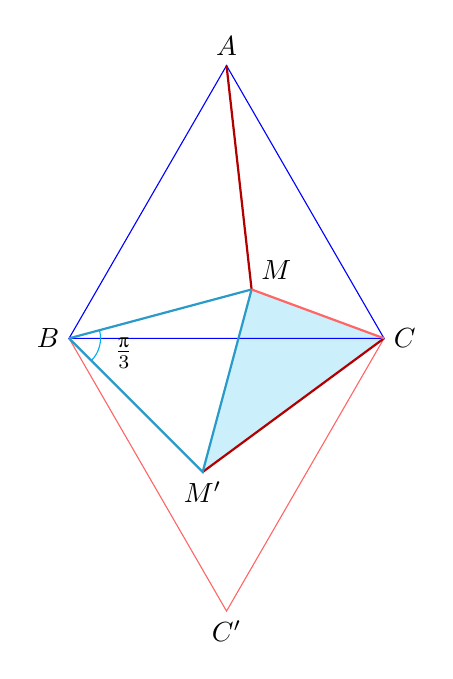
\begin{tikzpicture}[scale = 4]
      \draw (0,0) coordinate(B) node[left] {$B$}
        (1,0) coordinate(C) node[right]{$C$}
        (60:1) coordinate(A) node[above] {$A$}
        (-60:1) coordinate(C') node[below] {$C'$}
        (15:0.6) coordinate(M)node[above right]{$M$}
        (-45:0.6) coordinate(M')node[below]{$M'$};
      \fill [cyan,opacity=0.2] (C) -- (M) -- (M');
      \draw [blue] (B) -- (C) -- (A) -- cycle;
      \draw [red!60] (B) -- (C') -- (C);
      \draw [thick,red!70!black] (A) -- (M) (C) -- (M');
      \draw [thick,cyan!80!black] (B) -- (M)(M) -- (M') -- (B);
      \draw [thick,red!60] (C) -- (M);
      \tkzLabelAngle[pos=0.18](M',B,M){$\frac\pi3$}
      \tkzMarkAngle[cyan,size=0.1cm,mark=none](M',B,M)
    \end{tikzpicture}
    \caption{Pompeiu定理}\label{fig5.2}
  \end{minipage}
\end{figure}

\begin{solution}
  设$r=r_{B,-\frac\pi3}$表示绕着点$B$的角度为$\frac\pi3$的顺时针旋转. 则$r(A)=C,r(C)=C',r(M)=M'$,且点$B$是固定的. 我们有$\triangle MBM'$是等腰三角形,且由于$\angle  B=\frac\pi3$,我们得到$\triangle MBM'$是等边的. 因此,$\triangle CMM'$的边长等于线段$[MC],[MB]$和$[MA]$. 注意到$\triangle CMM'$是退化的,当且仅当$M$在$\triangle ABC$的外接圆上(图 \ref{fig5.2}).
\end{solution}

\begin{solution}
  设$r=r_{A,\frac\pi3}$表示绕着点$A$的角度为$\frac\pi3$的逆时针旋转,且令$C'=r(C),M'=r(M)$,其中$M$是$\triangle ABC$所在平面的任一点. 我们有$MA+MB+MC=BM+MM'+M'C'\ge BC'$,等号成立当且仅当点$B,M,M'$和$C'$是共线的. 由于$\triangle AMM'$是等边三角形,我们得到$\angle AMB=120^\circ,\angle AM'C'=120^\circ$.
  于是$\angle AMB=\angle AMC=120^\circ$. Torricelli点$T$的构造如下:我们在$\triangle ABC$外构造等边三角形$\triangle ACC'$和$\triangle AB'B$,我们有$\{T\}=BC'\cap CB'$(图 \ref{fig5.3}).
\end{solution}

\begin{figure}[!ht]
  \centering
  \caption{Torricelli点}\label{fig5.3}
  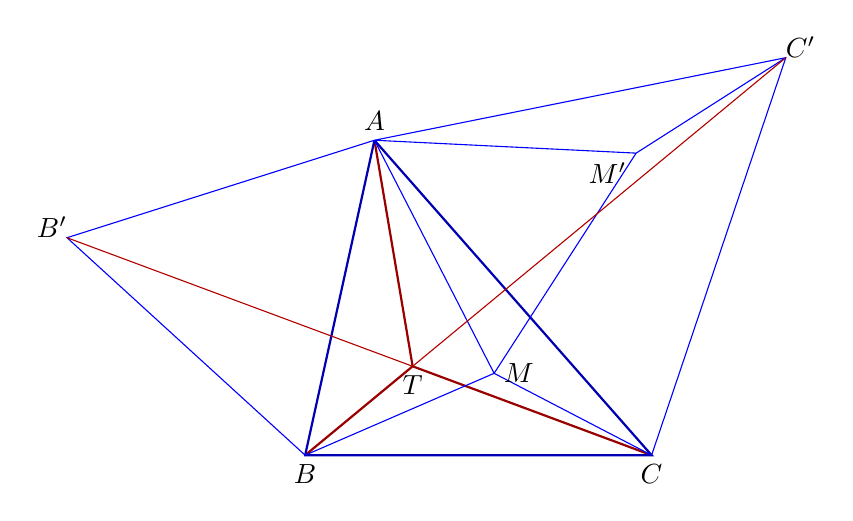
\begin{tikzpicture}[scale = 4]
    \tkzDefPoints{0/0/B, 1.1/0/C, 0.22/1/A, 0.6/0.26/M}
    \tkzDefEquilateral(B,A)
    \tkzGetPoint{B'}
    \tkzDefEquilateral(A,C)
    \tkzGetPoint{C'}
    \tkzDefEquilateral(A,M)
    \tkzGetPoint{M'}
    \tkzInterLL(C,B')(B,C')
    \tkzGetPoint{T}
    \draw [thick, red!60!black] (A) -- (T) (B) -- (T) (C) -- (T);
    \draw [thick, blue!70!black] (A) -- (B) -- (C) -- (A);
    \draw [blue] (A) -- (B') -- (B) (A) -- (C') -- (C) (A) -- (M) (B) -- (M) (C) -- (M) (A) -- (M') (M) -- (M') (C') -- (M');
    \draw [red!70!black] (B') -- (T) (C') -- (T);
    \tkzLabelPoints[below](B,C,T)
    \tkzLabelPoints[above](A)
    \tkzLabelPoints[above left=-5pt](B')
    \tkzLabelPoints[above right=-5pt](C')
    \tkzLabelPoints[below left](M')
    \tkzLabelPoints[right](M)
  \end{tikzpicture}
\end{figure}


\chapter{二次曲线}
\begin{proverb}
  { \itshape
   It is easy to teach someone, but to show him
   an easy way to realize the learned things, this
   is something to admire.
  }

\hfill St. John Chrysostom(347--407)
\end{proverb}

\section{二次曲线}
\begin{definition}
  代数平面曲线是其隐式方程为下列形式的曲线
  \[
    \mathscr C:\quad F(x,y) = 0,
  \]
  其中$F$是一个关于变量$x$和$y$的多项式. 多项式的次数称为代数曲线的次数.
\end{definition}

\begin{definition}
  二次曲线是次数为2的代数曲线. 二次曲线的一般方程为
  \[
    \mathscr C:\quad a_{11}x^2 + 2a_{12}xy + a_{22}y^2 + b_1x + b_2y + c = 0,
  \]
  其中$a_{11},a_{12},a_{22},b_1,b_2,c\in\MR$且$a_{11}^2+a_{12}^2
  +a_{22}^2\ne0$.
\end{definition}

当特殊选取平面坐标系的时候,二次曲线会有一个简单的形式,称为标准形. 我们回顾非退化的二次曲线.

{\noindent \kaishu 非退化的二次曲线}

\begin{itemize} \parindent=2em
  \item {\bfseries 椭圆} 定义成平面上到两个不同点$F(c,0)$和$F'(-c,0)$的距离之和为常数的点$M(x,y)$的集合,其中常数$c>0$称为{\kaishu 焦距}. 因此,满足性质$MF+MF'=2a.a>c$的点$M(x,y)$构成的集合$\mathscr E$叫做椭圆(图 \ref{fig6.1}).
      \begin{figure}[!ht]
        \centering
          \begin{tikzpicture}
    \draw [->] (-4,0) -- (-3,0) node[below left]
    {$A'$} -- (-2.236,0)node[below] {$F'$} -- (0,0)
    node[below left] {$O$} -- (2.236,0)node[below]
    {$F$} -- (3,0) node[below right] {$A$} -- (4,0)
    node[below] {$x$};
    \draw [->] (0,-3) -- (0,-2) node[below left]
    {$B'$} -- (0,2) node[above left]{$B$} -- (0,3)
    node[left] {$y$};
    \draw [domain=0:360,blue]
    plot({3*cos(\x)},{2*sin(\x)});
    \draw [red!70!black] (-2,0) --
    ({3*cos(60)},{2*sin(60)})node[above,black]{$M$}
    ({3*cos(60)},{2*sin(60)}) -- (2,0);
  \end{tikzpicture}

        \caption{椭圆$\frac{x^2}{a^2}+\frac{y^2}{b^2}=1,a,b>0$}\label{fig6.1}
      \end{figure}

      设$b^2=a^2-c^2$. 椭圆的方程为
      \begin{align*}
        & \mathscr E:\quad \frac{x^2}{a^2} + \frac{y^2}{b^2} = 1\quad \text{直接方程} \\
        & \mathscr E:\quad \left\{
           \begin{aligned}
             & y = \frac ba \sqrt{a^2 - x^2} \\
             & y = -\frac ba \sqrt{a^2 - x^2}
           \end{aligned}
           \right.,x\in[-a,a]\quad \text{笛卡尔方程} \\
        & \mathscr E:\quad \left\{
            \begin{aligned}
              & x = a\cos t \\
              & y = b\sin t
            \end{aligned}
          \right.,t\in[0,2\pi) \quad \text{参数方程}
      \end{align*}

     当$a=b=r$时,椭圆变成圆
     \[
       x^2 + y^2 = r^2 \quad \text{或} \quad
       \left\{
         \begin{aligned}
           & x = r \cos t \\
           & y = r \sin t
         \end{aligned}
       \right.,\quad t\in[0,2\pi).
     \]
     {\kaishu 光学性质.} 椭圆上一点的切线和法线是由{\kaishu 焦半径}确定的角的平分线.
  \item {\bfseries 双曲线} 定义成平面上到两个不同点$F(c,0)$和$F'(-c,0)$的距离之差的绝对值为常数的点$M(x,y)$的集合,其中常数$c>0$称为{\kaishu 焦距}. 因此,满足性质$|MF-MF'|=2a,0<a<c$的点$M(x,y)$的集合$\mathscr H$称为是双曲线(图 \ref{fig6.2}).
      \begin{figure}[!ht]
        \centering
          \begin{tikzpicture}
    \draw [->] (-6,0) -- (-3,0) node[below] {$F'$} -- (-2.236,0) node[below right] {$A'$} -- (0,0) node[below left] {$O$} -- (2.236,0) node[below left]{$A$} -- (3,0) node[below] {$F$} -- (6,0) node [below] {$x$};
    \draw [->] (0,-4) -- (0,4) node[left] {$y$};
    \draw [thick,blue,domain = -60:60] plot ({2.236*sec(\x)},{2*tan(\x)});
    \draw [thick,blue,xscale=-1, domain = -60:60] plot ({2.236*sec(\x)},{2*tan(\x)});
    \draw [blue!70!cyan,domain=-4:4] plot (\x,{2*\x/2.236}) node [above,black]{$y=\frac bax$};
    \draw [blue!70!cyan,domain=4:-4] plot (\x,{-2*\x/2.236})node [above,black]{$y=-\frac bax$};
    \draw [red!50!black] (-3,0) -- ({2.236*sec(45)},{2*tan(45)}) node[right,black]{$M$} -- (3,0);
  \end{tikzpicture}
        \caption{双曲线$\frac{x^2}{a^2}-\frac{y^2}{b^2}=1,a,b>0$}\label{fig6.2}
      \end{figure}

      由$F$和$F'$确定直线称为{\kaishu 焦轴},线段$FF'=2c$称为{\kaishu 焦距},线段$MF$和$MF'$称为{\kaishu 焦半径}. 直接计算可得双曲线的方程为:
      \begin{align*}
        & \mathscr H:\quad \frac{x^2}{a^2} - \frac{y^2}{b^2} = 1\quad \text{直接方程} \\
        & \mathscr H:\quad \left\{
           \begin{aligned}
             & y = \frac ba \sqrt{x^2 - a^2} \\
             & y = -\frac ba \sqrt{x^2 - a^2}
           \end{aligned}
           \right.,x\in(-\infty,-a]\cup[a,+\infty)\quad \text{笛卡尔方程} \\
        & \mathscr H:\quad \left\{
            \begin{aligned}
              & x = \pm a\cosh t \\
              & y = b\sinh t
            \end{aligned}
          \right.,t\in\MR \quad \text{参数方程}
      \end{align*}
      其中
      \[
        \cosh t = \frac{\ee^t + \ee^{-t}}2 \quad \text{且} \quad
        \sinh t = \frac{\ee^t - \ee^{-t}}2.
      \]
      双曲线是一个无界的曲线,其渐近线为$y=\frac bax$和$y=-\frac bax$. 渐近线互相正交的双曲线称为是等轴的.

      {\kaishu 光学性质.} 双曲线上一点的切线和法线是由焦半径确定的角的平分线.

    \item {\bfseries 抛物线} 定义成平面上到一个定直线$x=-\frac p2,p>0$和一个定点$F\left(\frac p2,0\right)$的距离相等的点$M(x,y)$的集合,其中定直线称为{\kaishu 准线},定点称为{\kaishu 焦点}(图 \ref{fig6.3}).
        \begin{figure}[!ht]
          \centering
            \begin{tikzpicture}[yscale = 0.8]
    \draw [->] (-2,0) -- (-1,0) node[below left] {$A$} -- (0,0) node[below left] {$O$} -- (1,0) node[below] {$F$} -- (5,0) node[below] {$x$};
    \draw [->] (0,-4) -- (0,4) node [left]{$y$};
    \draw [domain=-4:4,blue!60!black,semithick] plot (\x*\x/4,\x);
    \draw [blue!70!cyan] (-1,-4)node[above left,black] {$x=-\frac p2$} -- (-1,4);
    \draw [red!60!black](-1,2.8) node [left,black] {$B$} -- (1.96,2.8)node[above,black]{$M$} -- (1,0);
  \end{tikzpicture}
          \caption{抛物线$y^2=2px,p>0$}\label{fig6.3}
        \end{figure}

        因此,抛物线的方程为
        \begin{align*}
          & \mathscr P:\quad y^2 = 2px \quad \text{直接方程} \\
          & \mathscr P:\quad
            \left\{
              \begin{aligned}
                & x = \frac{t^2}{2p} \\
                & y = t
              \end{aligned}, t \in \MR\quad \text{参数方程}
            \right.
        \end{align*}
      一般地,抛物线也被定义成其函数图像具有以下形式:
      \[
        y = ax^2 + bx +c ,a\ne 0 \quad \text{或}\quad x = a'y^2 + b'y + c',a'\ne0.
      \]
      {\kaishu 光学性质.} 抛物线上一点的切线和法线是由焦点半径和通过该点到抛物线轴线的平行线确定的角的平分线.
\end{itemize}

{\noindent\kaishu 退化的二次曲线 }

二次代数曲线中退化的二次曲线为:
\begin{itemize}
  \item $\mathscr C:(a_1x+b_1y+c_1)(a_2x+b_2y+c_2)=0$(两条直线的并);
  \item $\mathscr C:\alpha(x-x_0)^2+\beta(y-y_0)^2=0,\alpha,
      \beta>0$(一个点);
  \item $\mathscr C:\alpha(x-x_0)^2+\beta(y-y_0)^2+\delta=0,
      \alpha,\beta,\delta>0$(空集).
\end{itemize}

利用初等几何可以得出二次曲线的基本性质,见 \cite{2}.

\section{化二次曲线为标准形}
设
\begin{equation}\label{eq6.1}
  \mathscr C:\quad a_{11}x^2 + 2a_{12}xy + a_{22}y^2 + b_1x + b_2y + c = 0,
\end{equation}
是在$xOy$面上的一个二次曲线,其中$a_{11},a_{12},a_{22},b_1,b_2,c\in\MR$且
$a_{11}^2+a_{12}^2+a_{22}^2\ne0$.

要将一个二次曲线化为其标准形,我们要在平面上选取一个坐标系,使得在新的坐标系下,二次曲线有一个简单的方程.,即所谓的约化方程. 我们将看到,任意一个这样的坐标变换由两个几何变换,即一个平移和一个旋转构成(和最后一个经过坐标轴的反射). 这些变换是基于二阶对称矩阵的Jordan标准形来决定的.

设$f(x,y)=a_{11}x^2+2a_{12}xy+a_{22}y^2$是方程 \eqref{eq6.1} 中的二次项部分,而$A_f$是$f$对应的对称矩阵
\[
  A_f = \begin{pmatrix}
    a_{11} & a_{12} \\
    a_{12} & a_{22}
  \end{pmatrix}.
\]
\begin{nota}
  在矩阵$A_f$的副对角线上的系数等于二次曲线中$xy$的系数的一半.
\end{nota}

熟知(定理 \ref{thm2.5})矩阵$A_f$是可对角化的,且可以取矩阵$P\in\MM_2(\MR)$是一个正交矩阵,即$P\TT=P^{-1}$. 事实上,$P$是一个旋转矩阵. $A_f$的特征值是实数$\lambda_1,\lambda_2$(见定理 \ref{thm2.5}),且其中至少有一个是非零的,因为$A_f\ne O_2$.

设
\[
  J_{A_f} = \begin{pmatrix}
    \lambda_1 & 0 \\
    0 & \lambda_2
  \end{pmatrix} = P\TT A_fP,
\]
其中$P$是由相应于特征值$\lambda_1$和$\lambda_2$的单位特征向量构成的矩阵.

{\bfseries 旋转.} 我们通过在$xOy$平面上进行正交变换来改变坐标系,由矩阵$P$定义的旋转为
\[
  \begin{pmatrix}
    x \\
    y
  \end{pmatrix} = P
  \begin{pmatrix}
    x' \\
    y'
  \end{pmatrix},
\]
则坐标系$xOy$变为$x'Oy'$.

利用公式
\[
  [f(x,y)] = \begin{pmatrix}
    x \\
    y
  \end{pmatrix}\TT A_f \begin{pmatrix}
    x \\
    y
  \end{pmatrix},
\]
我们得到
\[
  [f(x,y)] = \left( P\begin{pmatrix}
    x' \\
    y'
  \end{pmatrix} \right)\TT A_f P
  \begin{pmatrix}
    x' \\
    y'
  \end{pmatrix} =
  \begin{pmatrix}
    x' \\
    y'
  \end{pmatrix}\TT J_{A_f}
  \begin{pmatrix}
    x' \\
    y'
  \end{pmatrix} =
  \lambda_1x'^2 + \lambda_2y'^2.
\]
因此,在新坐标系$x'Oy'$下,二次曲线的方程变为
\begin{equation}\label{eq6.2}
  \mathscr C:\quad \lambda_1 x'^2 + \lambda_2y'^2 + b_1'x' + b_2'y' + c = 0,
\end{equation}
其中系数$b_1',b_2'$由公式
\[
  b_1x + b_2y = b_1'x' + b_2'y'\quad \Leftrightarrow
  \quad [b_1\,b_2]\begin{pmatrix}
    x \\
    y
  \end{pmatrix} = [b_1'\,b_2']
  \begin{pmatrix}
    x' \\
    y'
  \end{pmatrix}
\]
所决定,这等价于
\[
  [b_1\,b_2] P \begin{pmatrix}
    x' \\
    y'
  \end{pmatrix} =
  [b_1'\,b_2'] \begin{pmatrix}
    x' \\
    y'
  \end{pmatrix}, \quad \text{所以} \quad
  [b_1'\,b_2'] = [b_1\,b_2]P.
\]

\begin{nota}
  旋转的目的是使得$xy$的项消失.
\end{nota}

{\bfseries 平移.} 我们分$A_f$是特征值都非零和其中有一个为零的两种情形.

{\kaishu 情形1.} 如果$\lambda_1\ne0$且$\lambda_2\ne0$,我们将方程 \eqref{eq6.2} 写成
\[
  \mathscr C :\quad \lambda_1\left( x' + \frac{b_1'}{2\lambda_1} \right)^2 + \lambda_2
  \left( y' + \frac{b_2'}{2\lambda_2} \right)^2 + c' = 0,
\]
其中
\[
  c' = c - \frac{b_1'^2}{4\lambda_1} - \frac{b_2'^2}{4\lambda_2}.
\]

现在我们平移坐标系$x'Oy'$到坐标系$x''O''y''$,平移公式为
\[
  T:\left\{
    \begin{aligned}
      & x'' = x' + \frac{b_1'}{2\lambda_1} \\
      & y'' = y' + \frac{b_2'}{2\lambda_2}
    \end{aligned}
  \right..
\]

新坐标系的中心为$O''$,其坐标满足
\[
  x'' = y'' =0 \quad \Leftrightarrow \quad
  x' = - \frac{b_1'}{2\lambda_1},y' = - \frac{b_2'}{2\lambda_2} \quad \Leftrightarrow \quad
  \begin{pmatrix}
    x \\
    y
  \end{pmatrix} = P
  \begin{pmatrix}
    x' \\
    y'
  \end{pmatrix}.
\]
二次曲线的方程变为
\[
  \mathscr C:\quad \lambda_1x''^2 + \lambda_2y''^2 + c' = 0.
\]

如果$c'=0$,我们得到一个退化的二次曲线,它是一个点或两条直线的并.

如果$c'\ne0$,二次曲线或者是椭圆,或者是双曲线,取决于特征值$\lambda_1,\lambda_2$是否具有相同的符号.

{\bfseries 情形2.} 如果其中一个特征值为0,不妨设$\lambda_2=0$
且$\lambda_1\ne0$,我们有
\[
  \mathscr C: \quad \lambda_1 \left( x' + \frac{b_1'}{2\lambda_1} \right)^2 + b_2'y' + c' = 0,\quad c' = c - \frac{b_1'^2}{4\lambda_1},
\]
在这种情形下, 平移公式为
\[
  T: \left\{
    \begin{aligned}
      & x'' = x' + \frac{b_1'}{2\lambda_1} \\
      & y'' = y' + \frac{c'}{b_2'}
    \end{aligned}
  \right..
\]
此二次曲线是一个抛物线,其方程为
\[
  \mathscr C:\quad \lambda_1x''^2 + b_2'y'' = 0.
\]
\begin{nota}
  平移公式是在完成对$x'$或$y'$的配方之后所决定的.
\end{nota}

\begin{remark}
  如果二次曲线是非退化的,则其类型只需要通过分析$A_f$的特征值的符号即可得到. 确切地讲,如果

  $\lambda_1\lambda_2>0$,则二次曲线为椭圆;

  $\lambda_1\lambda_2<0$,则二次曲线为双曲线;

  $\lambda_1\lambda_2=0$,则二次曲线为抛物线.
\end{remark}

现在我们总结上面使用的技巧,并给出一个化二次曲线为标准形的算法.

\begin{mybox}
  {\bfseries 化二次型为标准形的算法}

  \begin{itemize}
    \item {\bfseries 步骤1.} 写出矩阵$A_f$并求出其特征值.
    \item {\bfseries 步骤2.} 求出Jordan标准形$J_{A_f}$和正交矩阵$P,P\TT=P^{-1}$,其满足等式
        \[
          J_{A_f} = \begin{pmatrix}
            \lambda_1 & 0 \\
            0 & \lambda_2
          \end{pmatrix} = P\TT A_fP.
        \]
    \item {\bfseries 步骤3.} 将旋转公式写成
        \[
          X = PY,\quad \text{其中} \quad
          X = \begin{pmatrix}
            x \\
            y
          \end{pmatrix} \quad \text{且} \quad
          Y = \begin{pmatrix}
            x' \\
            y'
          \end{pmatrix}.
        \]
        写出$P=R_\alpha$,求出旋转角. 因此,坐标系$xOy$逆时针旋转角度$\alpha$变成了坐标系$x'Oy'$.
    \item {\bfseries 步骤4.} 对$x'$或$y'$完成配方以后写出平移公式.
    \item {\bfseries 步骤5.} 分析关于$x''$和$y''$的方程来确定二次曲线的类型.
  \end{itemize}
\end{mybox}

\begin{example}
  {\bfseries 双曲线.} 我们考虑二次曲线
  \[
    \mathscr C: \quad 3x^2 + 10xy + 3y^2 - 2x - 14y - 13 = 0,
  \]
  我们将其化为标准形,并决定其类型(图 \ref{fig6.4}).
\end{example}
\begin{figure}[!ht]
  \centering
  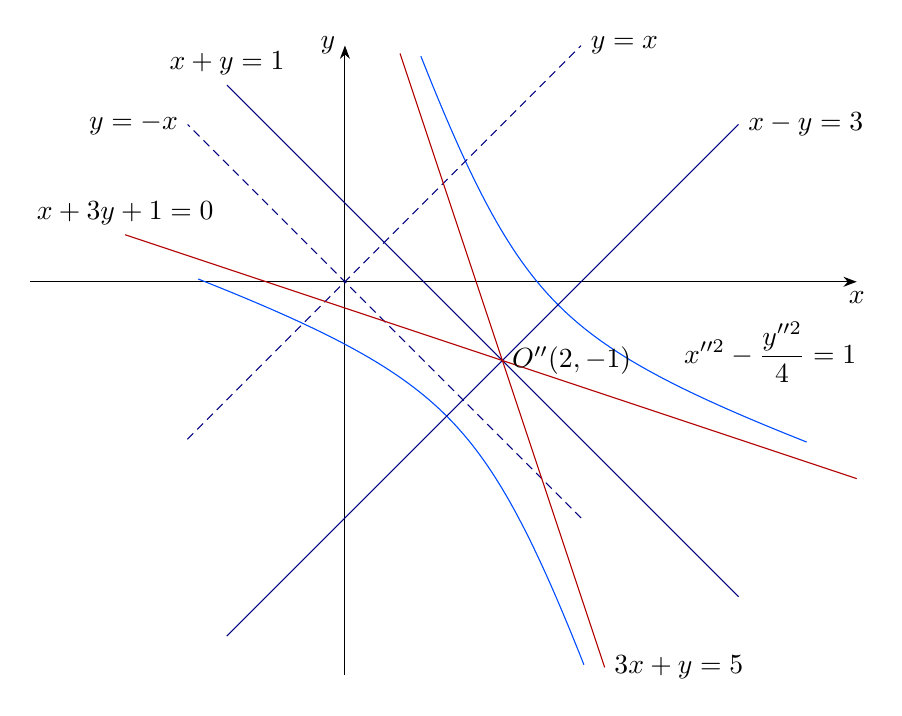
\begin{tikzpicture}[every node/.style={black}]
  \draw [->] (-4,0) -- (6.5,0) node [below] {$x$};
  \draw [->] (0,-5) -- (0,3) node [left] {$y$};
  \begin{scope}[shift = {(2,-1)},blue!70!cyan]
    \draw [rotate = 45,domain=-60:60] plot ({sec(\x)},{2*tan(\x)});
    \draw [rotate = 45,domain=-60:60] plot ({-sec(\x)},{2*tan(\x)});
  \end{scope}
  \draw [blue!50!black] plot[domain=-1.5:5] (\x,\x-3) node[right] {$x-y=3$}
  plot[domain = 5:-1.5] (\x,1-\x)node[above] {$x+y=1$};
  \draw [densely dashed,blue!50!black,domain = -2:3] plot[domain = 3:-2] (\x,-\x)node[left] {$y=-x$} plot(\x,\x) node[right]{$y=x$};
  \draw [red!70!black] plot [domain = -2.5:0.6] (-3*\x-1,\x) node[above] {$x+3y+1=0$}
  plot [domain = 0.7:3.3] (\x,5-3*\x) node [right]{$3x+y=5$};
  \node at (5.4,-0.9) {$\displaystyle x''^2-\frac{y''^2}4=1$};
  \node [right] at (2,-1) {$O''(2,-1)$};
\end{tikzpicture} 
  \caption{双曲线$3x^2+10xy+3y^2-2x-14y-13=0$}\label{fig6.4}
\end{figure}

{\bfseries 步骤1.} 与二次曲线对应的二次型为$f(x,y)=3x^2+10xy+3y^2$,其相应的对称矩阵为
\[
  A_f = \begin{pmatrix}
    3 & 5 \\
    5 & 3
  \end{pmatrix}.
\]

$A_f$的特征值通过解方程$\det(A_f-\lambda I_2)=0$得到,这意味着$(3-\lambda)^2-25=0\Rightarrow\lambda_1=8,\lambda_2=-2$.

{\bfseries 步骤2.} 我们求出相应于特征值$\lambda_1=8$和$\lambda_2=-2$的特征向量. 相应于特征值$\lambda_1=8$的特征向量要解方程$(A_f-8I_2)X=0$,我们有
\[
  \left\{
    \begin{aligned}
      & -5x_1 + 5x_2 = 0 \\
      & 5x_1 - 5x_2 = 0
    \end{aligned}
  \right.,
\]
这意味着$x_1=x_2$,方程组的解为$\begin{pmatrix}
  \alpha \\
  \alpha
\end{pmatrix},\alpha\in\MR^\ast$. 我们设$\alpha=1$,并将这里的向量除以它的范数(长度),我们得到特征向量
\[
  X_1 = \begin{pmatrix}
    \frac1{\sqrt2} \\
    \frac1{\sqrt2}
  \end{pmatrix}.
\]

类似地,相应于$\lambda_2=-2$的特征向量要解方程组$(A_f+2I_2)X=0$,我们得到特征向量
\[
  X_2 = \begin{pmatrix}
    -\frac1{\sqrt2} \\
    \frac1{\sqrt2}
  \end{pmatrix}.
\]

因此,
\[
  P = \begin{pmatrix}
    \frac1{\sqrt2} & - \frac1{\sqrt2} \\
    \frac1{\sqrt2} & \frac1{\sqrt2}
  \end{pmatrix} =
  \begin{pmatrix}
    \cos\frac\pi4 & - \sin\frac\pi4 \\
    \sin\frac\pi4 & \cos \frac\pi4
  \end{pmatrix} = R_{\frac\pi4},
\]
这是角度为$\frac\pi4$的旋转矩阵.

{\bfseries 步骤3.} 旋转公式为
\begin{equation}\label{eq6.3}
  \begin{pmatrix}
    x \\
    y
  \end{pmatrix} = P
  \begin{pmatrix}
    x' \\
    y'
  \end{pmatrix} \quad \text{或} \quad
  \left\{
    \begin{aligned}
      & x = \frac1{\sqrt2}x' - \frac1{\sqrt2}y' \\
      & y = \frac1{\sqrt2}x' + \frac1{\sqrt2}y'
    \end{aligned}
  \right..
\end{equation}

我们将坐标系$xOy$逆时针旋转角度$\frac\pi4$,则二次曲线的方程变为
\[
  \mathscr C;\quad 8x'^2 - 2y'^2 - \frac2{\sqrt2}(x' - y') - \frac{14}{\sqrt2}(x' + y') - 13 = 0,
\]

{\bfseries 步骤4.}  平移公式为
\[
  T: \left\{
    \begin{aligned}
      & x'' = x - \frac1{\sqrt2} \\
      & y'' = y' + \frac3{\sqrt2}
    \end{aligned}
  \right..
\]
因此,我们将坐标系$x'Oy'$平移到$x''O''y''$,二次曲线的方程变为
\[
  \mathscr C:\quad 8x''^2 - 2y''^2 - 8 = 0 \quad \Leftrightarrow \quad x''^2 - \frac{y''^2}4 = 1.
\]
于是,我们二次曲线是一个双曲线,半轴长分别为$a=1$和$b=2$.

接下来,我们求出方程的对称轴和坐标系的中心$O'$.

由 \eqref{eq6.3},我们有$\begin{pmatrix}
  x' \\
  y'
\end{pmatrix}=P^{-1}\begin{pmatrix}
  x \\
  y
\end{pmatrix}=P\TT\begin{pmatrix}
  x \\
  y
\end{pmatrix}$,而这意味着
\begin{equation}\label{eq6.4}
  \left\{
    \begin{aligned}
      & x' = \frac1{\sqrt2} (x + y) \\
      & y' = \frac1{\sqrt2} (-x + y)
    \end{aligned}
  \right..
\end{equation}

{\kaishu $O''x''$的方程.} 要求出$O''x''$的方程,我们令$y''=0$,这反过来说明$y'=-\frac3{\sqrt2}$. \eqref{eq6.4} 的第二个方程说明$-x+y=-3$.

{\kaishu $O''y''$的方程.}  要求出$O''y''$的方程,我们令$x''=0$,这意味着$x'=\frac1{\sqrt2}$. 然而, \eqref{eq6.4} 中的第一个方程意味着$x+y=1$.

{\kaishu 对称中心$O''$的坐标.} $O''$的坐标是方程组
\[
  \left\{
    \begin{aligned}
      & x + y = 1\\
      & -x + y = -3
    \end{aligned}
  \right.
\]
的解,这说明$x=2,y=-1$. 因此,$O''(2,-1)$,即$O''$在坐标系$xOy$下的坐标为$(2,-1)$.

\section{问题}
\begin{problem}
  求出下面二次曲线的标准形,判断其类型,求出对称轴及其中心:
  \begin{enumerate}[left=0cm,align=right,label=(\arabic*)]
    \item $3x^2-4xy+3y^2-2x-2y+1=0$;
    \item $2x^2-4xy-y^2+\sqrt5x+\sqrt5y-1=0$;
    \item $x^2-2xy+y^2+2x-4y+5=0$;
    \item $4x^2+12xy+9y^2-64=0$;
    \item $9x^2+24xy+16y^2-40x+30y=0$;
    \item $2x^2-6xy+10y^2-8x+12y+2=0$;
    \item $4x^2-4xy+y^2-2x-14y+7=0$;
    \item $4xy-3y^2+4x-14y-7=0$;
    \item $3x^2-4xy-2x+4y-3=0$;
    \item $x^2+2xy+y^2+2x+2y-3=0$;
    \item $x^2-8xy+7y^2+6x-6y+9=0$;
    \item $5x^2+12xy-22x-12y-19=0$;
    \item $6x^2-4xy+9y^2-4x-32y-6=0$;
    \item $5x^2+4xy+8y^2-32x-56y+80=0$;
    \item $xy-k=0,k\in\MR^\ast$.
  \end{enumerate}
\end{problem}

\begin{problem}
  根据参数$a$的值,讨论下列二次曲线的类型:
  \begin{enumerate}[left=0cm,align=right,label=(\arabic*)]
    \item $5x^2+2axy+5y^2+2x+2y+2=0$;
    \item $ax^2+2xy+ay^2-2x+2y+9=0$;
    \item $x^2+4xy+4y^2+ax=0$;
    \item $7x^2-8xy+y^2+a=0$.
  \end{enumerate}
\end{problem}

\begin{problem}
  对怎样的$c$,笛卡尔方程$2xy-4x+6y+c=0$表示一对直线?
\end{problem}

\begin{problem}
  {\kaishu 等轴双曲线.} 证明:二次曲线$(x+2y+1)(2x-y+1)+\alpha=0,\alpha\ne0$是一个双曲线,且其渐近线为$x+2y+1=0$和$2x-y+1=0$.
\end{problem}

\begin{remark}
  更一般地,我们可以证明二次曲线
  \[
    (a_1x + b_1y + c_1)(a_2x + b_2y + c_2) + \alpha = 0,a_1b_2 - a_2b_1\ne0,\alpha\ne0
  \]
  是一个双曲线,且其渐近线为$a_1x+b_1y+c_1=0$和$a_2x+b_2y+c_2=0$.
\end{remark}

\begin{problem}
  \begin{inparaenum}[(a)]
    \item 求出经过点$(1,1),(2,1)$和$(-1,-2)$,且以$x+y-1=0$为渐近线的双曲线的方程.

    \item 求出过点$(1,1)$和$(2,1)$,且以$x-y+1=0$为渐近线的等轴双曲线的方程.
  \end{inparaenum}
\end{problem}

\begin{mybox}
  \begin{problem}[一个Lam\'e曲线和一个伪装的抛物线.]
  
    设实数$k>0$,证明曲线:$\mathscr C_k^1:\sqrt y - \sqrt x = \sqrt k,\mathscr C_k^2:\sqrt x+\sqrt y=\sqrt k$和$\mathscr C_k^3:\sqrt x-\sqrt y=\sqrt k$合起来构成了一个抛物线,求出其标准形,顶点和对称轴.
  \end{problem}
\end{mybox}

\begin{remark}
  一个{\kaishu Lam\'e曲线}\index{L!Lam\'e曲线}的笛卡尔方程为$\frac{x^\alpha}{a^\alpha}+\frac{y^\alpha}{b^\alpha}=1$,其中$a,b$是正实数,而$\alpha$为实数. 这类曲线被G.Lam\'e \cite{39} 在19世纪所研究,现在它们被称为{\kaishu Lam\'e曲线}或{\kaishu 超椭圆}.

  当$k=1$时,曲线$\mathscr C_1^2$在 \cite{12} 中讨论了,它说明虽然$\mathscr C_1^2$看起来像是圆弧,但实际上$\mathscr C_1^2$是双曲线的一部分.
\end{remark}

\begin{problem}
  求出二次曲线$\mathscr C:x^2+y^2-4xy-1=0$的类型,并求出$\mathscr C$上的格点.
\end{problem}

\begin{problem}
  证明双曲线$\mathscr H$:$x^2-5y^2=4$包含无穷多个格点.
\end{problem}

\begin{problem}
  \begin{inparaenum}[(a)]
    \item\label{prob6.9a} 求出$xOy$平面上的一个椭圆,其焦点为$F_1(\sqrt3,2),F_2(3\sqrt3,4)$,且长半轴为$a=3$.

    \item 求出 (\ref{prob6.9a}) 中二次曲线的标准形.
  \end{inparaenum}
\end{problem}

\begin{problem}
  \begin{inparaenum}[(a)]
    \item\label{prob6.10a} 求出焦点为$F_1(-1,2),F_2(3,6)$,半轴为$a=2$的双曲线方程.

    \item 求出 (\ref{prob6.10a}) 中二次曲线的标准形.
  \end{inparaenum}
\end{problem}

\begin{problem}
  \begin{inparaenum}[(a)]
    \item\label{prob6.11a} 求出$xOy$平面上到直线$\mathscr D:\sqrt3x-3y+2\sqrt3=0$和到点$F(2,0)$距离相等的点$M(x,y)$的轨迹.

    \item 求出 (\ref{prob6.11a}) 中二次曲线的标准形.
  \end{inparaenum}
\end{problem}

\begin{problem}[\kaishu 由椭圆决定的Abel群.]

设$\mathscr E$表示椭圆$\frac{x^2}{a^2}+\frac{y^2}{b^2}=1$,且设$\ast$是一个作用于$\mathscr E$的二元算符,其定义为$\ast:\mathscr E\times\mathscr E\to\mathscr E,(M_1,M_2)\in\mathscr E\times\mathscr E\to
M_1\ast M_1\in\mathscr E$,其中$M_1\ast M_2$是过点$A(a,0)$且平行于线段$[M_1M_2]$的直线与椭圆$\mathscr E$的交点. 证明$(\mathscr E,\ast)$是一个Abel群.
\end{problem}

\begin{problem}
  求函数$f(x,y)=x^2+xy+y^2+x-y-1$的最值以及对应的极值点.
\end{problem}

\begin{problem}[\kaishu 带限制条件的极值问题.]

  \begin{inparaenum}[(a)]
    \item 求函数$f(x,y)=x+y$在条件$3x^2-2xy+3y^2+4x+4y-4=0$下的最大值和最小值.

    \item 求函数$f(x,y)=2x+y$在条件$3x^2+10xy+3y^2-16x-16y-16=0$下的极值.

    \item 求函数$f(x,y)=2x-y$在条件$9x^2+24xy+16y^2-40x+30y=0$下的极值.
  \end{inparaenum}
\end{problem}

\begin{mybox}
  \begin{problem}[一个二次型的条件极值.]

    设函数$f(x,y)=ax^2+2bxy+cy^2,a,b,c\in\MR$满足$a^2+b^2+c^2\ne0$. 证明:函数$f$在条件$x^2+y^2=1$下的最小值和最大值分别是矩阵
    \[
      A_f = \begin{pmatrix}
        a & b \\
        b & c
      \end{pmatrix}
    \]
    的最小和最大特征值.
  \end{problem}
\end{mybox}

\begin{problem}
  求出由曲线
  \[
    5x^2 + 6xy + 5y^2 - 16x - 16y - 16 = 0
  \]
  所围成区域的面积.
\end{problem}

{\noindent \kaishu 椭圆域上的二重积分.}

\begin{problem}
  计算:
  \begin{enum}
    \item $\iint_{D_1}\ee^{x^2-xy+y^2}\dif x\dif y$,其中$D_1=\{(x,y)\in\MR^2:x^2-xy+y^2\le1\}$;
    \item $\iint_{D_2}\ee^{x^2+xy+y^2}\dif x\dif y$,其中$D_2=\{(x,y)\in\MR^2:x^2+xy+y^2\le1\}$;
    \item $\iint_{D_3}\ee^{-x^2+xy-y^2}\dif x\dif y$,其中$D_3=\{(x,y)\in\MR^2:x^2-xy+y^2\ge1\}$;
    \item $\iint_{D_4}\ee^{-x^2-xy-y^2}\dif x\dif y$,其中$D_4=\{(x,y)\in\MR^2:x^2+xy+y^2\ge1\}$.
  \end{enum}
\end{problem}

\begin{problem}
  设$a,b\in\MR$满足$0<b<2a$,且设$\alpha>0$. 计算:
  \begin{enum}
    \item $\iint_{D_1}\ee^{ax^2-bxy+ay^2}\dif x\dif y$,其中$D_1=\{(x,y)\in\MR^2:ax^2-bxy+ay^2\le\alpha\}$;
    \item $\iint_{D_2}\ee^{ax^2+bxy+ay^2}\dif x\dif y$,其中$D_2=\{(x,y)\in\MR^2:ax^2+bxy+ay^2\le\alpha\}$;
    \item $\iint_{D_3}\ee^{-ax^2+bxy-ay^2}\dif x\dif y$,其中$D_3=\{(x,y)\in\MR^2:ax^2-bxy+ay^2\ge\alpha\}$;
    \item $\iint_{D_3}\ee^{-ax^2-bxy-ay^2}\dif x\dif y$,其中$D_4=\{(x,y)\in\MR^2:ax^2+bxy+ay^2\ge\alpha\}$.
  \end{enum}
\end{problem}

\begin{mybox}
  \begin{problem}
    设$ab\in\MR$满足$0<b<2a$,且设$\alpha>0$. 计算:
    \begin{enum}
      \item \label{prob6.19a} $\iint_{D_\alpha}x\ee^{-ax^2-bxy-ay^2}\dif x\dif y$;
      \item \label{prob6.19b} $\iint_{D_\alpha}xy\ee^{-ax^2-bxy-ay^2}\dif x\dif y$,
    \end{enum}
    其中$D_\alpha=\{(x,y)\in\MR^2,ax^2+bxy+ay^2\ge\alpha\}$.
  \end{problem}
\end{mybox}

\begin{mybox}
  \begin{problem}[二次型和特殊积分.]

    \begin{inparaenum}[(a)]
      \item 计算
      \[
        \iint_{\MR^2} \frac{\dif x\dif y}{(1+3x^2-4xy+3y^2)^3}.
      \]

      \item 设$A\in\MM_2(\MR)$是一个具有正特征值的对称矩阵,且设实数$\alpha>1$. 证明:
      \[
        \iint_{\MR^2} \frac{\dif x\dif y}{(1+v\TT Av)^\alpha} = \frac\pi{(\alpha-1)\sqrt{\det A}},\quad \text{其中} \quad v = \begin{pmatrix}
          x \\
          y
        \end{pmatrix}.
      \]

      \item 设$f$是$[0,+\infty)$上的一个可积函数,且设$\int_0^{+\infty}f(x)\dif x=I$. 证明:如果$A\in\MM_2(\MR)$是一个具有正特征值的对称矩阵,则
          \[
            \iint_{\MR^2}f\left( v\TT Av \right) =
            \frac{\pi I}{\sqrt{\det A}}, \quad
            \text{其中} \quad v = \begin{pmatrix}
               x \\
               y
             \end{pmatrix}.
          \]
    \end{inparaenum}
  \end{problem}
\end{mybox}

\begin{mybox}
  \begin{problem}[一个特殊情形和一个公式.]

    \begin{inparaenum}[(a)]
      \item 计算
      \[
        \iint_{\MR^2} \ee^{-(3x^2 - 2xy + 3y^2 + 2x + 2y - 1)}\dif x \dif y.
      \]

      \item\label{prob6.21b} 设$A\in\MM_2(\MR)$是一个具有正特征值的对称矩阵,$b=\begin{pmatrix}
            b_1 \\
            b_2
          \end{pmatrix}$是$\MR^2$中的一个特征向量,$c$是一个实数. 证明:
          \[
            \iint_{\MR^2} \ee^{-(v\TT Av + 2b\TT v+c)}\dif x\dif y = \frac\pi{\sqrt{\det A}} \ee^{b\TT A^{-1}b-c},\quad \text{其中} \quad v = \begin{pmatrix}
               x \\
               y
             \end{pmatrix}.
          \]
    \end{inparaenum}
  \end{problem}
\end{mybox}

\section{解答}
\begin{solution}
  \begin{inparaenum}[(1)]
    \item 椭圆$x''^2+5y''^2=1$,坐标轴$O''x''$的方程为$x-y=0$,$O''y''$的方程为$x+y=2$,中心为$O''(1,1)$;

    \item 双曲线$48x''^2-72y''^2=1$,坐标轴$O''x''$的方程为$-2x+y=\frac{\sqrt5}6$,$O''y''$的方程为$x+2y=\frac{3\sqrt5}4$,中心为$O''\left(\frac{\sqrt5}{12},
        \frac{\sqrt5}3\right)$;

    \item 抛物线$x''-\sqrt2y''^2=0$,坐标轴$O''x''$的方程为$-x+y=\frac32$,$O''y''$的方程为$x+y=\frac{11}4$,中心为$O''\left(\frac58,\frac{17}8\right)$;

    \item 二次曲线退化为两条平行直线$(2x+3y-8)(2x+3y+8)=0$;

    \item 抛物线$x'^2+2y'=0$,坐标轴$Ox'$的方程为$-4x+3y=0$,$Oy'$的方程为$3x+4y=0$,中心为$O(0,0)$;

    \item 椭圆$x''^2+11y''^2-6=0$,坐标轴$O''x''$的方程为$x-3y=2$,$O''y''$的方程为$3x+y=6$,中心为$O''(2,0)$;

    \item 双曲线$y''^2-\frac6{\sqrt5}x''=0$,坐标轴$O''x''$的方程为$-x+2y=1$,$O''y''$的方程为$x+2y=1$,中心为$O''\left(-\frac15,\frac35\right)$;

    \item 双曲线$-x''^2+4y''^2-4=0$,坐标轴$O''x''$的方程为$-x+2y=-4$,$O''y''$的方程为$2x+y=3$,中心为$O''(2,-1)$;

    \item 双曲线$-x''^2+4y''^2=2$,坐标轴$O''x''$的方程为$2x-y=1$,$O''y''$的方程为$x+2y=3$,中心为$O''(1,1)$;

    \item 二次曲线退化为两条平行直线$(x+y-1)(x+y+3)=0$;

    \item 双曲线$\frac{x''^2}9-y''^2=1$,坐标轴$O''x''$的方程为$-x+2y=1$,$O''y''$的方程为$2x+y=3$,中心为$O''(1,1)$;

    \item 双曲线$\frac{x''^2}4-\frac{y''^2}9=1$,坐标轴$O''x''$的方程为$-2x+3y=1$,$O''y''$的方程为$3x+2y=5$,中心为$O''(1,1)$;

    \item 椭圆$\frac{x''^2}8+\frac{y''^2}4=1$,坐标轴$O''x''$的方程为$-x+2y=3$,$O''y''$的方程为$2x+y=4$,中心为$O''(1,2)$;

    \item 椭圆$\frac{x''^2}4+\frac{y''^2}9=1$,坐标轴$O''x''$的方程为$2x-y=1$,$O''y''$的方程为$x+2y=8$,中心为$O''(2,3)$;

    \item 等轴双曲线$x'^2-y'^2-2k=0$,它以$x$轴和$y$轴为渐近线. 如果$k>0$,则双曲线的两个分支分别在第一和第三象限,如果$k<0$,则双曲线的两个分支分别在第二和第四象限.
  \end{inparaenum}
\end{solution}

\begin{solution}
  \begin{inparaenum}[(1)]
    \item 与二次曲线对应的矩阵为$A=\begin{pmatrix}
      5 & a \\
      a & 5
    \end{pmatrix}$,其特征值为$\lambda_1=5-a,\lambda_2=5+a$. 如果$a\ne0$,则相应于特征值$\lambda_1=5-a$和$\lambda_2=5+a$的特征向量为$X_1=\frac1{\sqrt2}\begin{pmatrix}
      1 \\
      -1
    \end{pmatrix}$和$X_2=\frac1{\sqrt2}\begin{pmatrix}
      1 \\
      1
    \end{pmatrix}$,且$P=\frac1{\sqrt2}\begin{pmatrix}
      1 & 1\\
      -1 & 1
    \end{pmatrix}=R_{-\frac\pi4}$,这是一个角度为$-\frac\pi4$的旋转.
  \end{inparaenum}
  \begin{itemize}
    \item 如果$a=0$,则二次曲线的方程变为$\mathscr C:5x^2+5y^2+2x+2y+2=0\Leftrightarrow \mathscr C:4x^2+4y^2+(x+1)^2+(y+1)^2=0\Rightarrow \mathscr C=\varnothing$.
    \item 如果$a=5$,我们有$\mathscr C:5x^2+10xy+5y^2+2x+2y+2=0\Leftrightarrow \mathscr C:4(x+y)^2+(x+y+1)^2+1=0\Rightarrow\mathscr C=\varnothing$.
    \item 如果$a=-5$,则二次曲线的方程变为$\mathscr C:5x^2-10xy+5y^2+2x+2y+2=0\Leftrightarrow
        \mathscr C:5(x-y)^2+2(x-y)+4y+2=0\Leftrightarrow
        \mathscr C:5\left(x-y+\frac15\right)^2=-4\left(y+
        \frac9{20}\right)$,这是一个抛物线.
  \end{itemize}

  我们作旋转$\begin{pmatrix}
    x \\
    y
  \end{pmatrix}=P\begin{pmatrix}
    x' \\
    y'
  \end{pmatrix}$,且二次曲线的方程变为$(5-a)x'^2+(5+a)y'^2+2\sqrt2y'+2=0$或者
  \[
    \mathscr C:\quad (5 - a)x'^2 + (5 + a)\left( y'^2 + \frac{2\sqrt2}{5 + a}y' + \frac2{(5 + a)^2}\right) + 2\frac{4 + a}{5 + a} = 0.
  \]
  \begin{itemize}
    \item 如果$a=-4$,则二次曲线的方程变为$\mathscr C:\frac92(x-y)^2+\frac12(x+y+2)^2=0$,且二次曲线退化为一个点$\mathscr C=\{(-1,-1)\}$.
    \item 如果$a\in(-5,-4)$,我们有$5-a>0,5+a>0,\frac{4+a}{5+a}<0$,这说明$\mathscr C$是一个椭圆.
    \item 如果$a\in(-4,5)$,我们有$5-a>0,5+a>0,\frac{4+a}{5+a}>0\Rightarrow\mathscr C=\varnothing$.
    \item 如果$a\in(-\infty,-5)\cup(5,+\infty)$,由于$5+a$和$5-a$的符号相反,我们得到$\mathscr C$是一个双曲线.
  \end{itemize}

  综上所述:
  \begin{itemize}
    \item 如果$a\in(-\infty,-5)\cup(5,+\infty)\Rightarrow\mathscr C $是一个双曲线.
    \item 如果$a=-5\Rightarrow\mathscr C$是一个抛物线.
    \item 如果$a\in(-5,-4)\Rightarrow\mathscr C$是一个椭圆.
    \item 如果$a=-4\Rightarrow\mathscr C$退化为一个点.
    \item 如果$a\in(-4,5]\Rightarrow\mathscr C$是空集.
  \end{itemize}

  \begin{inparaenum}[(1)]\setcounter{enumi}{1}
    \item 与二次曲线对应的矩阵为$A=\begin{pmatrix}
      a & 1 \\
      1 & a
    \end{pmatrix}$,其特征值为$\lambda_1=a+1,\lambda_2=a-1$. 相应的特征向量为$X_1=\frac1{\sqrt2}\begin{pmatrix}
      1 \\
      1
    \end{pmatrix}$和$X_2=\frac1{\sqrt2}\begin{pmatrix}
      -1 \\
      1
    \end{pmatrix}$,且$P=\frac1{\sqrt2}\begin{pmatrix}
      1 & -1\\
      1 & 1
    \end{pmatrix}=R_{\frac\pi4}$,这是一个角度为$\frac\pi4$的旋转.
  \end{inparaenum}
  \begin{itemize}
    \item 如果$a=1$,我们有$(x+y)^2-2(x+y)+1=-4y-8\Leftrightarrow
        (x+y-1)^2=-4(y+2)$,这是一个抛物线.
    \item 如果$a=-1$,我们有$\mathscr C:(x-y+1)^2=10\Leftrightarrow \mathscr C:x-y+1=\pm\sqrt{10}$,二次曲线退化为两条直线的并.
    \item 如果$a\in\MR\backslash\{\pm1\}$,我们作旋转$\begin{pmatrix}
          x \\
          y
        \end{pmatrix}=P\begin{pmatrix}
          x' \\
          y'
        \end{pmatrix}$,且二次曲线的方程变为$(a+1)x'^2+(a-1)y'^2+2\sqrt2y'+9=0$. 我们通过对$y'$配方得到
        \[
          (a + 1)x'^2 + (a - 1)\left( y' + \frac{\sqrt2}{a-1} \right)^2 + \frac{9a-11}{a-1} = 0.
        \]
    \end{itemize}

  我们分以下几种情形:
  \begin{itemize}
    \item 如果$a=\frac{11}9$,由于$a+1>0,a-1>0$,二次曲线退化为点$\left(\frac92,-\frac92\right)$.
    \item 如果$a>\frac{11}9$,由于$a+1>0,a-1>0,\frac{9a-11}{a-1}>0$,二次曲线退化为空集.
    \item 如果$a\in\left(1,\frac{11}9\right)$,则$a+1>0,a-1>0,\frac{9a-11}{a-1}<0$,二次曲线是椭圆.
    \item 如果$a\in(-1,1)$,则$ a+1>0,a-1<0,\frac{9a-11}{a-1}>0$,二次曲线是双曲线.
    \item 如果$a\in(-\infty,-1)$,则$ a+1<0,a-1<0,\frac{9a-11}{a-1}>0$,二次曲线是椭圆.
  \end{itemize}

  综上所述:
  \begin{itemize}
    \item 如果$a\in(-\infty,-1)\cup\left(1,\frac{11}9\right)$,二次曲线是一个椭圆.
    \item 如果$a=-1$,则二次曲线是两条直线的并.
    \item 如果$a\in(-1,1)$,则二次曲线是一个双曲线.
    \item 如果$a=1$,则二次曲线是一个抛物线.
    \item 如果$a=\frac{11}9$,则二次曲线退化为一个点.
    \item 如果$a\in\left(\frac{11}9,+\infty\right)$,则二次曲线是空集.
  \end{itemize}

  \begin{inparaenum}[(1)]\setcounter{enumi}{2}
    \item 我们有$x^2+4xy+4y^2+ax=0\Leftrightarrow (x+2y)^2=-ax$. 如果$a=0$,则二次曲线退化为直线$x+2y=0$;如果$a\ne0$,则二次曲线为抛物线.

    \item 与二次曲线对应的矩阵为$A=\begin{pmatrix}
      7 & -4 \\
      -4 & 1
    \end{pmatrix}$,其特征值为$\lambda_1=9,\lambda_2=-1$. 作旋转$X=PY$,二次曲线的方程变为$9x'^2-y'^2+a=0$. 如果$a\ne0$,则二次曲线为双曲线;如果$a=0$,则二次曲线退化为两条直线的并. 由于$7x^2-8xy+y^2=0\Leftrightarrow (x-y)(7x-y)=0$,这意味着$x-y=0$或$7x-y=0$. 因此,当$a=0$时,我们有$\mathscr C=\mathscr D_1\cup\mathscr D_2$,其中$\mathscr D_1:x-y=0$,$D_2:7x-y=0$.
  \end{inparaenum}
\end{solution}

\begin{solution}
  $c=-12$.
\end{solution}

\setcounter{solution}{4}

\begin{solution}
  \begin{inparaenum}[(a)]
    \item 由注 \ref{remark6.2},以$x+y-1=0$为渐近线的双曲线的方程为$(ax+by+c)(x+y-1)+\alpha=0,\alpha\ne0$. 由于点$(1,1),(2,1)$和$(-1,-2)$在双曲线的图像上,我们有线性方程组
        \[
          \left\{
            \begin{aligned}
              & a + b + c + \alpha = 0 \\
              & 4a + 2b + 2c + \alpha = 0 \\
              & 4a + 8b - 4c + \alpha = 0
            \end{aligned}
          \right..
        \]
        这说明双曲线的方程为$(2x-3y-3)(x+y-1)+4=0$.

    \item 由于等轴双曲线具有互相垂直的渐近线,我们得到双曲线的方程为$(x+y+c)(x-y+1)+\alpha=0,\alpha\ne0$. 于是$(x+y-4)(x-y+1)+2=0$.
  \end{inparaenum}
\end{solution}

\begin{solution}
  我们考虑曲线$\mathscr C_k^2:\sqrt x+\sqrt y=\sqrt k$,且注意到$x,y\in[0,k]$. 我们将方程两边平方,得到$x+y+2\sqrt{xy}=k\Leftrightarrow 2\sqrt{xy}=k-x-y$,这说明$k\ge x+y$. 且由于$x,y\in[0,k]$,我们可知曲线包含在一个以$A(0,k),B(k,0)$和$O(0,0)$为顶点的三角形内. 将之前的方程再平方,得到$x^2-2xy+y^2-2kx-2ky+k^2=0$. 因此,曲线是二次曲线,确切地说,是包含在$\triangle OAB$内的一个二次曲线的弧,即
  \[
    \mathscr C_k^2:\quad x^2 - 2xy + y^2 - 2kx - 2ky + k^2 = 0,\quad 0\le x\le k,\quad 0\le y\le k.
  \]
  二次型$x^2=2xy+y^2$的矩阵为$A=\begin{pmatrix}
    1 & -1\\
    -1 & 1
  \end{pmatrix}$,其特征值为$\lambda_1=0,\lambda_2=2$,相应的特征值为
  \[
    X_1 = \begin{pmatrix}
      \frac1{\sqrt2} \\
      \frac1{\sqrt2}
    \end{pmatrix} \quad \text{和} \quad
    X_2 = \begin{pmatrix}
      -\frac1{\sqrt2} \\
      \frac1{\sqrt2}
    \end{pmatrix}.
  \]
  旋转矩阵$P=\begin{pmatrix}
    \frac{\sqrt2}2 & - \frac{\sqrt2}2 \\
    \frac{\sqrt2}2 & \frac{\sqrt2}2
  \end{pmatrix}=R_{\frac\pi4}$. 我们作旋转,旋转公式为$X=PY$,
  \[
    \left\{
      \begin{aligned}
        & x = \frac1{\sqrt2}x' - \frac1{\sqrt2}y' \\
        & y = \frac1{\sqrt2}x' + \frac1{\sqrt2}y'
      \end{aligned}
    \right. \quad \text{或} \quad
    \left\{
      \begin{aligned}
        & x' = \frac1{\sqrt2}x - \frac1{\sqrt2}y \\
        & y' = -\frac1{\sqrt2}x + \frac1{\sqrt2}y
      \end{aligned}
    \right..
  \]
  二次曲线在坐标系$x'O'y'$下的方程为$y'^2-\sqrt2kx'+\frac{k^2}2=0\Leftrightarrow y'^2-\sqrt2k\left(x-\frac k{2\sqrt2}\right)=0$. 平移公式为$x''=x'-\frac k{2\sqrt2},y''=y'$,将二次曲线化为标准形,在坐标系$x''O''y''$下的方程为$y''^2-\sqrt2kx''=0$. 这是一个抛物线,所以曲线$\mathscr C_k^2$是抛物线的弧,它与$x$轴和$y$轴相切,且包含在$\triangle OAB$内.

  新坐标系的轴$O''x'':y''=0\Leftrightarrow y'=0\Leftrightarrow x-y=0$,轴$O''y'':x''=0\Leftrightarrow x'=\frac k{2\sqrt2}\Leftrightarrow x+y=\frac k2$. 抛物线的顶点,即这两条轴的交点坐标为$\left(\frac k4,\frac k4\right)$.

  类似地,我们可以证明另外两条曲线$\mathscr C_k^1$和$\mathscr C_k^3$也是抛物线,即$\mathscr C_k^1$是抛物线在直线$y-x=0$上方的无界弧,它与$y$轴在$A(0,k)$处相切. 而$\mathscr C_k^3$是在直线$y-x=0$下方的无界弧,它与$x$轴在$B(k,0)$处相切( 图 \ref{fig6.5}).
\end{solution}

\begin{figure}[!ht]
  \centering
  \begin{tikzpicture}[every node/.style={black},scale=1.3]
    \draw [->] (-2.7,0) -- (0,0)node[below left] {$O$} -- (1,0) node [below] {$B(k,0)$} -- (4,0) node[below] {$x$};
    \draw [->] (0,-1) -- (0,1)node[left] {$A(0,k)$} -- (0,4) node [left] {$y$};
    \begin{scope}[shift={(0.5,0.5)}]
      \draw [rotate=45,domain=-sqrt(2)/2:sqrt(2)/2,blue!60!black] plot({\x*\x/sqrt(2)-sqrt(2)/4},\x);
      \draw [rotate=45,domain=-sqrt(2)/2:-2,blue!60!cyan] plot({\x*\x/sqrt(2)-sqrt(2)/4},\x) node[above]{$\sqrt y-\sqrt x=\sqrt k$};
      \draw [rotate=45,domain=sqrt(2)/2:2,blue!60!cyan] plot({\x*\x/sqrt(2)-sqrt(2)/4},\x) node[above right=-3pt]{$\sqrt x-\sqrt y=\sqrt k$};
    \end{scope}
    \draw [domain=0:3,red!50] plot (\x,\x);
    \draw [densely dashed,red!60!black] (0,1) -- (1,0);
    \draw [->] (-1.5,0.3) node[fill=white,inner sep=0pt]{$\sqrt x+\sqrt y=\sqrt k$} -- (0.15,0.3);
  \end{tikzpicture}
  \caption{Lam\'e抛物线}\label{fig6.5}
\end{figure}

\begin{solution}
  相应于$\mathscr C$的二次型矩阵为$A=\begin{pmatrix}
    1 & -2 \\
    -2 & 1
  \end{pmatrix}$,其特征值为$\lambda_1=3,\lambda_1=-1$. 由于$\lambda_1\lambda_2<0$,二次曲线为双曲线. 我们将二次曲线的方程写成$(x-2y)^2-3y^2=1$,且注意到这是一个Pell方程,其最小解为$x_0=4,y_0=1$. 此方程的通解满足$x_n-2y_n+y_n\sqrt3=(2+\sqrt3)^n$,这意味着
  \[
    x - 2y_n = \frac{(2+\sqrt3)^n+(2-\sqrt3)^n}2 \quad \text{且} \quad
    y_n = \frac{(2+\sqrt3)^n-(2-\sqrt3)^n}{2\sqrt3},\;n\ge 1.
  \]
  此双曲线上的格点为$(\pm1,0)$和$(\pm x_n,\pm y_n)$,其中
  \begin{align*}
    & x_n = \left( \frac12 + \frac1{\sqrt3} \right) (2 + \sqrt3)^n + \left( \frac12 - \frac1{\sqrt3} \right)(2 - \sqrt3)^n , \\
    & y_n = \frac1{2\sqrt3} (2 + \sqrt3)^n - \frac1{2\sqrt3} (2 - \sqrt3)^n,\; n\ge1.
  \end{align*}
\end{solution}

\begin{solution}
  直接计算可知$(2,0),(3,1)$和$(7,3)$都在抛物线上. 我们来求出矩阵$A\in\MM_2(\MQ)$,使得通过递推关系
  \[
    \begin{pmatrix}
      x_{n+1} \\
      y_{n+1}
    \end{pmatrix} = A
    \begin{pmatrix}
      x_n \\
      y_n
    \end{pmatrix}, n\ge0
  \]
  可以生成无穷多个格点$(x_n,y_n)\in\mathscr H$. 设$\begin{pmatrix}
    x_0 \\
    y_0
  \end{pmatrix}=\begin{pmatrix}
    2 \\
    0
  \end{pmatrix},\begin{pmatrix}
    x_1 \\
    y_1
  \end{pmatrix}=\begin{pmatrix}
    3 \\
    1
  \end{pmatrix}$且$\begin{pmatrix}
    x_2 \\
    y_2
  \end{pmatrix}=\begin{pmatrix}
    7 \\
    3
  \end{pmatrix}$. 我们有$\begin{pmatrix}
    3 \\
    1
  \end{pmatrix}=A\begin{pmatrix}
    2 \\
    0
  \end{pmatrix},\begin{pmatrix}
    7 \\
    3
  \end{pmatrix}=A\begin{pmatrix}
    3 \\
    1
  \end{pmatrix}$,于是$\begin{pmatrix}
    3 & 7 \\
    1 & 3
  \end{pmatrix}=A\begin{pmatrix}
    2 & 3 \\
    0 & 1
  \end{pmatrix}$. 这说明$A=\frac12\begin{pmatrix}
    3 & 5 \\
    1 & 3
  \end{pmatrix}$. 矩阵递推关系说明$x_{n+1}=\dfrac12(3x_n+5y_n)$,且
  $y_{n+1}=\frac12(x_n+3y_n),n\ge0$. 我们可以验证$x_{n+1}^2-5y_{n+1}^2=x_n^2-5y_n^2=4,\forall n\ge0$,所以对任意$n\ge0$,$(x_n,y_n)\in\mathscr H$.
\end{solution}

\begin{solution}
  \begin{inparaenum}[(a)]
    \item 椭圆的中心是线段$[F_1F_2]$的中点$O''(2\sqrt3,3)$. 椭圆的长半轴在直线$F_1F_2$上,其方程为$O''x'':y=\frac1{\sqrt3}x+1$. 短半轴经过点$O''$且垂直于$O''x''$,其方程为$O''y'':y=-\sqrt3x+9$. $Ox$与$O''x''$的夹角由直线$O''x''$的斜率决定,即$m=\frac1{\sqrt3}=\tan\frac\pi6$,所以坐标系$x''O''y''$可以将标准坐标系$xOy$旋转角度$\frac\pi6$后再经过一次把原点$O(0,0)$移到$O''(2\sqrt3,3)$的平移得到. 点$M(x,y)$在坐标系$x''O''y''$下的坐标$(x'',y'')$满足
        \begin{equation}\label{eq6.5}
          \begin{pmatrix}
            x'' \\
            y''
          \end{pmatrix} =
          \begin{pmatrix}
            \frac{\sqrt3}2 & \frac12 \\
            -\frac12 & \frac{\sqrt3}2
          \end{pmatrix}
          \begin{pmatrix}
            x - 2\sqrt 3\\
            y - 3
          \end{pmatrix}.
        \end{equation}
    此椭圆的焦距为$F_1F_2=4$,所以$c=2,a=3$,且$b^2=a^2-c^2=5$. 椭圆在坐标系$x''O''y''$下的方程为$\mathscr C:\frac{x''^2}9+\frac{y''^2}5-1=0$. 利用等式 \eqref{eq6.5},我们得到$x''=\frac12(\sqrt3x+y-9),
    y''=\frac12(-x+\sqrt3y-\sqrt3)$,然后将它们带入椭圆的方程,我们得到$\mathscr C:6x^2+8y^2-2\sqrt3xy-18\sqrt3x-36y+63=0$.

    \item 椭圆所对应的二次型的矩阵为$A=\begin{pmatrix}
      6 & - \sqrt3 \\
      -\sqrt3 & 8
    \end{pmatrix}$,其特征值为$\lambda_1=5,\lambda_2=9$,相应的特征向量为$X_1=\begin{pmatrix}
      \frac{\sqrt3}2 \\
      \frac12
    \end{pmatrix}$和$X_2=\begin{pmatrix}
      -\frac{\sqrt3}2 \\
      \frac12
    \end{pmatrix}$. 使得$A$化为Jordan标准形的矩阵$P=\begin{pmatrix}
      \frac{\sqrt3}2 & - \frac12 \\
      \frac12 & \frac{\sqrt3}2
    \end{pmatrix}=R_{\frac\pi6}$. 我们绕原点作角度为$\frac\pi6$的旋转,得到坐标系$x'Oy'$. 在此坐标系下,椭圆$\mathscr C$上的点$(x,y)$的坐标$(x',y')$满足公式
    \[
      \begin{pmatrix}
        x \\
        y
      \end{pmatrix} =
      \begin{pmatrix}
      \frac{\sqrt3}2 & - \frac12 \\
      \frac12 & \frac{\sqrt3}2
    \end{pmatrix}
    \begin{pmatrix}
        x' \\
        y'
      \end{pmatrix}.
    \]
    不需要计算,可知二次曲线的二次型$6x^2+88y^2-2\sqrt3xy$变为$5x'^2+9y'^2$,根据上述公式计算二次曲线中的一次项,我们得到二次曲线在新坐标系$x'Oy'$下的方程为$\mathscr C:5x'^2+9y'^2-45x'-9\sqrt3y'+63=0$,即$\mathscr C:5\left(x'-\frac92\right)^2+
    9\left(y'-\frac{\sqrt3}2\right)^2-45=0$. 我们作平移$x''=x'-\frac92,y''=y'-\frac{\sqrt3}2$,我们得到一个新的坐标系$x''O''y''$,二次曲线在坐标系$x''O''y''$下的方程变为$\frac{x''^2}9+\frac{y''^2}5-1=0$,这和我们在 (\ref{prob6.9a}) 中得到的方程相同.

    新坐标系的坐标轴为$O''x'':y''=0\Leftrightarrow y'=\frac{\sqrt3}2\Leftrightarrow x-\sqrt3y-\sqrt3=0$和$O''y'':x''=0\Leftrightarrow
    x'=\frac92\Leftrightarrow \sqrt3x+y-9=0$. 椭圆的中心,是两条坐标轴的交点,即$O''(2\sqrt3,3)$. 因此,二次曲线是椭圆,且半轴分别为$a=3,b=\sqrt5$.
  \end{inparaenum}
\end{solution}

\begin{solution}
  \begin{inparaenum}[(a)]
    \item 双曲线的中心是线段$[F_1F_2]$的中点,即$O''(1,4)$. 焦距为$F_1F_2=4\sqrt2$,所以$c=4\sqrt2,a=2$且$b^2=c^2-a^2=4$,这意味着双曲线是等轴的. 我们取坐标系$x''O''y''$使得$x''$轴是直线$F_1F_2$,其方程为$O''x'':y=x+3$,而$y''$轴经过点$O''$且垂直于$x''$轴,其方程为$O''y'':y=-x+5$. 在新坐标系$x''O''y''$下,双曲线的方程为$\frac{x''^2}4-\frac{y''^2}4-1=0
        \Leftrightarrow x''^2-y''^2-4=0$. 坐标系$x''O''y''$可通过将坐标系$xOy$旋转角度$\frac\pi4$以后再将$O$平移到$O''$处得到. 在坐标系$xOy$下的点$M(x,y)$在新坐标系$x''O''y''$下的坐标$(x'',y'')$满足公式
        \[
          \begin{pmatrix}
            x'' \\
            y''
          \end{pmatrix} =
          R_{-\frac\pi4}
          \begin{pmatrix}
            x - 1 \\
            y - 4
          \end{pmatrix} =
          \begin{pmatrix}
            \frac{\sqrt2}2 & \frac{\sqrt2}2 \\
            -\frac{\sqrt2}2 & \frac{\sqrt2}2
          \end{pmatrix}
          \begin{pmatrix}
            x - 1 \\
            y - 4
          \end{pmatrix}.
        \]
    于是$x''=\frac{\sqrt2}2(x+y-5),y''=\frac{\sqrt2}2(-x+y
    -3)$,并将它们带入$x''^2-y''^2-4=0$,我们得到双曲线在坐标系$xOy$下的方程为$xy-4x-y-2=0$.

    \item 我们将二次曲线的方程写成$\mathscr C:2xy-8x-2y+4=0$,且注意到相应于二次型$2xy$的矩阵为$A=\begin{pmatrix}
          0 & 1 \\
          1 & 0
        \end{pmatrix}$,其特征值为$\lambda_1=1,\lambda_2=-1$,而相应的特征向量为$X_1=\begin{pmatrix}
          \frac{\sqrt2}2 \\
          \frac{\sqrt2}2
        \end{pmatrix}$和$X_2=\begin{pmatrix}
          -\frac{\sqrt2}2 \\
          \frac{\sqrt2}2
        \end{pmatrix}$. 使得矩阵$A$化为Jordan标准形的矩阵$P=\begin{pmatrix}
            \frac{\sqrt2}2 & -\frac{\sqrt2}2 \\
            \frac{\sqrt2}2 & \frac{\sqrt2}2
          \end{pmatrix}=R_{\frac\pi4}$. 我们作旋转坐标变换$\begin{pmatrix}
            x \\
            y
          \end{pmatrix}=R_{\frac\pi4}
          \begin{pmatrix}
            x' \\
            y'
          \end{pmatrix}$,我们得到二次曲线在坐标系$x'Oy'$下的方程为$x'^2-y'^2-5\sqrt2x'-3\sqrt2y'+4=0\Leftrightarrow
          \left(x'-\frac{5\sqrt2}2\right)^2-
          \left(y'-\frac{3\sqrt2}2\right)^2-4=0$. 这意味着$\frac{x''^2}4-\frac{y''^2}4-1=0$,其中$x''=x'-\frac{5\sqrt2}2,y''=y'-\frac{3\sqrt2}2$.

          新坐标系的坐标轴为$O''x'':y''=0\Leftrightarrow y=x+3$和$O''y'':x''=0\Leftrightarrow y=-x+5$. 双曲线的中心,是这两条坐标轴的交点$O''(1,4)$.
  \end{inparaenum}
\end{solution}

\begin{solution}
  \begin{inparaenum}[(a)]
    \item 轨迹是以$\mathscr D$为准线,以$F$为焦点的抛物线,抛物线的对称轴是过$F$且垂直于$\mathscr D$的直线. $\mathscr D$的斜率为$m=\frac{\sqrt3}3$,则对称轴的斜率为$m'=-\frac1m=-\sqrt3$,于是对称轴的方程为$\mathscr D':y=-\sqrt3(x-2)$. $F$在准线上的投影为点$F'(1,\sqrt3)$,它是直线$\mathscr D$与$\mathscr D'$的交点,$FF'=2$,所以$p=4$.

        抛物线在新坐标系下的方程为$\mathscr P:y''^2=2px''$,其中心是线段$[FF']$的中点,即$O''\left(\frac32,\frac{\sqrt3}2\right)$,且坐标轴为$O''x''=\mathscr D':y=-\sqrt3(x+2)$和$O''y'':x-\sqrt3y=0$,且$O''y''$平行于$\mathscr D$. 在坐标系$x''O''y''$下,抛物线的方程为$y''^2=8x''$. 坐标轴$O''x''$与$Ox$的夹角由$\mathscr D'$的斜率给出,即$m=\tan\alpha=-\sqrt3$,所以$\alpha=-\frac\pi3$. 因此,坐标系$x''O''y''$可通过角度为$-\frac\pi3$的旋转和沿着向量$OO''$的平移得到. 在坐标系$xOy$下的点$M(x,y)$在新坐标系$x''O''y''$下的坐标$(x'',y'')$满足公式
        \[
          \begin{pmatrix}
            x'' \\
            y''
          \end{pmatrix} = R_{\frac\pi3}
          \begin{pmatrix}
            x - \frac32 \\
            y - \frac{\sqrt3}2
          \end{pmatrix} =
          \begin{pmatrix}
            \frac12 & -\frac{\sqrt3}2 \\
            \frac{\sqrt3}2 & \frac12
          \end{pmatrix}
          \begin{pmatrix}
            x - \frac32 \\
            y - \frac{\sqrt3}2
          \end{pmatrix}.
        \]
    我们得到抛物线的方程为
    \[
      \mathscr D:\quad 3x^2 + y^2 + 2\sqrt3xy - 28x + 12\sqrt3y + 12 = 0.
    \]

    \item 相应于二次型$3x^2+y^2+2\sqrt3xy$的矩阵为$A=\begin{pmatrix}
          3 & \sqrt 3 \\
          \sqrt 3 & 1
        \end{pmatrix}$,其特征值为$\lambda_1=0,\lambda_2=4$,相应的特征向量为$X_1=\begin{pmatrix}
          \frac12 \\
          -\frac{\sqrt3}2
        \end{pmatrix}$和$X_2=\begin{pmatrix}
          \frac{\sqrt3}2 \\
          \frac12
        \end{pmatrix}$. 使得矩阵$A$化为Jordan标准形的矩阵$P=\begin{pmatrix}
          \frac12 & \frac{\sqrt3}2 \\
          -\frac{\sqrt3}2 & \frac12
        \end{pmatrix}=R_{-\frac\pi3}$. 我们将坐标系$xOy$旋转角度$-\frac\pi3$,我们得到坐标系$x'Oy'$,且有公式
        \[
          \begin{pmatrix}
            x \\
            y
          \end{pmatrix} =
          R_{-\frac\pi3}
          \begin{pmatrix}
            x' \\
            y'
          \end{pmatrix} \quad
          \text{或} \quad
          \begin{pmatrix}
            x' \\
            y'
          \end{pmatrix} =
          R_{\frac\pi3}
          \begin{pmatrix}
            x \\
            y
          \end{pmatrix}.
        \]
    二次曲线在坐标系$x'Oy'$下的方程为$y'^2-2\sqrt3y'+3=8x'\Leftrightarrow(y'-\sqrt3)^2
    =8x'\Leftrightarrow y'^2=8x''$,其中$x''=x',y''=y'-\sqrt3$.

    新坐标系的坐标轴为$O''x'':y''=0\Leftrightarrow y'=\sqrt3\Leftrightarrow \sqrt3x+y-2\sqrt3=0$,这是直线$\mathscr D'$,以及$O''y'':x''=0\Leftrightarrow x'=0\Leftrightarrow x-\sqrt3y=0$. 坐标系的中心是这两条坐标轴的交点$O''\left(\frac32,\frac{\sqrt3}2\right)$.
  \end{inparaenum}
\end{solution}

\begin{solution}
  设$M_1(a\cos t_1,b\sin t_1)$和$M_2(a\cos t_2,b\sin t_2)$,且$M_1\ast M_2=M(a\cos t,b\sin t)$. 直线$M_1M_2$的斜率为$m=\frac{b\sin t_2-\sin t_1}{a\cos t_2-\cos t_1}=-\frac ba\cot\frac{t_1+t_2}2$. 过点$A$且平行于$M_1M_2$的直线方程为$\mathscr D:y=-\frac ba\cot\frac{t_1+t_2}2(x-a)$. 将此直线与椭圆相交,我们得到方程$b\sin t=\frac ba\cot\frac{t_1+t_2}2a(\cos t-1)\Leftrightarrow \sin\frac t2\cos\frac t2=\sin^2\frac t2\cot\frac{t_1+t_2}2$. 当$\sin\frac t2=0$,我们得到点$A$,当$\sin\frac t2\ne0$,我们有$\tan\frac t2=\tan\frac{t_1+t_2}2$,所以$t=t_1+t_2$.

  二元算符$\ast$满足结合律,因为$M(t_1)\ast\big(M(t_2)\ast M(t_3)\big)=\big(M(t_1)\ast M(t_2)\big)\ast M(t_3)=M(t_1+t_2+t_3)$. 还满足交换律,因为$M(t_1)\ast M(t_2)=M(t_2)\ast M(t_1)=M(t_1+t_2)$.  $\ast$的单位元是$A=M(0)$,$M(t)$关于$\ast$的逆元为$M'(-t)$,这是$M$关于$x$轴的对称点.
\end{solution}

\begin{solution}
  与函数$f(x,y)$对应的二次型$2x^2+2xy+2y^2$的矩阵为$A=\begin{pmatrix}
    2 & 1 \\
    1 & 2
  \end{pmatrix}$,其特征值为$\lambda_1=3,\lambda_2=1$,相应的特征向量为$v_1=\begin{pmatrix}
    \frac1{\sqrt2} \\
    \frac1{\sqrt2}
  \end{pmatrix}$和$v_2=\begin{pmatrix}
    -\frac1{\sqrt2} \\
    \frac1{\sqrt2}
  \end{pmatrix}$,于是
  \[
    J_A = \begin{pmatrix}
      3 & 0 \\
      0 & 1
    \end{pmatrix} \quad \text{且} \quad
    P = \begin{pmatrix}
      \frac1{\sqrt2} & - \frac1{\sqrt2} \\
      \frac1{\sqrt2} & \frac1{\sqrt2}
    \end{pmatrix}.
  \]
  我们作旋转变换
  \[
    \left\{
      \begin{aligned}
        & x = \frac1{\sqrt2}x' - \frac1{\sqrt2}y' \\
        & y = \frac1{\sqrt2}x' + \frac1{\sqrt2}y'
      \end{aligned}
    \right.,
  \]
  可得函数$2f$在坐标系$x'Oy'$下的表达式为$g(x',y')=3x'^2+y'^2-2\sqrt2y'-2
  =3x'^2+(y'-\sqrt2)^2-4 $. 函数$g$在$(0,\sqrt2)$处取最小值$-4$,于是$f$在$(x,y)=(-1,1)$处取最小值$f(-1,1)=-2$.
\end{solution}

\begin{solution}
  \begin{inparaenum}[(a)]
    \item 二次型$3x^2-2xy+3y^2$的矩阵为$A=\begin{pmatrix}
          3 & -1 \\
          -1 & 3
        \end{pmatrix}$,其特征值为$\lambda_1=2,\lambda_2=4$,相应的特征向量为$v_1=\begin{pmatrix}
          \frac1{\sqrt2} \\
          \frac1{\sqrt2}
        \end{pmatrix}$和$v_2=\begin{pmatrix}
          -\frac1{\sqrt2} \\
          \frac1{\sqrt2}
        \end{pmatrix}$,于是
        \[
          J_A = \begin{pmatrix}
            2 & 0 \\
            0 & 4
          \end{pmatrix} \quad \text{且} \quad
          P = \begin{pmatrix}
            \frac1{\sqrt2} & - \frac1{\sqrt2} \\
            \frac1{\sqrt2} & \frac1{\sqrt2}
          \end{pmatrix}.
        \]

       我们作旋转变换
       \[
         \left\{
           \begin{aligned}
             & x = \frac1{\sqrt2}x' - \frac1{\sqrt2}y' \\
             & y = \frac1{\sqrt2}x' + \frac1{\sqrt2}y'
           \end{aligned}
         \right.,
       \]
    二次曲线的方程变为$x'^2+2y'^2+2\sqrt2x'-2=0\Leftrightarrow (x'+\sqrt2)^2+2y'^2=4$,作平移$x'+\sqrt2=x'',y'=y''$之后可得二次曲线为椭圆$x''^2+2y''^2=4$. 椭圆的参数方程为$x''=2\cos t.y''=\sqrt2\sin t,t\in[0,2\pi)$. 利用旋转和平移的公式,我们得到
    \[
      \left\{
        \begin{aligned}
          & x = \sqrt2\cos t - \sin t - 1 \\
          & y = \sqrt2\cos t + \sin t - 1
        \end{aligned}
      \right.,
    \]
    其中$t\in[0,2\pi)$. 于是$f(x,y)=g(t)=2\sqrt2\cos t-2,t\in[0,2\pi)$,此函数当$t=\pi$时取最小值$-2\sqrt2-2$,当$t=0$时取最大值$2\sqrt2-2$. 因此,函数$f$在限制条件下的全局最小值在$(-\sqrt2-1,-\sqrt2-1)$处取到,为$-2\sqrt2-2$;全局最大值在$(x,y)=(\sqrt2-1,\sqrt2-1)$处取到,为$2\sqrt2-2$.

    \begin{nota}
      设$\mathscr E$表示椭圆$3x^2-2xy+3y^2+4x+4y-4=0$. 值得一提的是,由于$f$是一个连续函数,而$\mathscr E$是一个紧集. 由Weierstrass定理,$f|_{\mathscr E}$存在全局最小值和最大值. 利用Lagrange乘数法,我们只需求出限制条件下$f$的驻点,在这里的情形中有两个这样的点,然后只需要观察其中一个是最小值点,另一个是最大值点.
    \end{nota}

    \item 二次型$3x^2+10xy+3y^2$的矩阵为$A=\begin{pmatrix}
          3 & 5 \\
          5 & 3
        \end{pmatrix}$,其特征值为$\lambda_1=8,\lambda_2=-2$,相应的特征向量为
        $ v_1=\begin{pmatrix}
          \frac1{\sqrt2} \\
          \frac1{\sqrt2}
        \end{pmatrix}$和$v_2=\begin{pmatrix}
          -\frac1{\sqrt2} \\
          \frac1{\sqrt2}
        \end{pmatrix}$,于是
        \[
          J_A = \begin{pmatrix}
            8 & 0 \\
            0 & -2
          \end{pmatrix} \quad \text{且} \quad
          P = \begin{pmatrix}
            \frac1{\sqrt2} & - \frac1{\sqrt2} \\
            \frac1{\sqrt2} & \frac1{\sqrt2}
          \end{pmatrix}.
        \]

       旋转
       \[
         \left\{
           \begin{aligned}
             & x = \frac1{\sqrt2}x' - \frac1{\sqrt2}y' \\
             & y = \frac1{\sqrt2}x' + \frac1{\sqrt2}y'
           \end{aligned}
         \right.,
       \]
       和平移
       \[
         \left\{
           \begin{aligned}
             & x' - \sqrt2 = x'' \\
             & y' = y''
           \end{aligned}
         \right.
       \]
       说明我们的二次曲线为双曲线$4x''^2-y''^2=16$.

       设$\mathscr H$表示此双曲线,而$\mathscr H_1$和$\mathscr H_2$是$\mathscr H$的两个分支,即$\mathscr H=\mathscr H_1\cup\mathscr H_2$.

       $\mathscr H_1$的参数方程为$x''=2\cosh t,y''=4\sinh t,t\in\MR$. 我们得到旋转和平移方程为
       \[
         \left\{
           \begin{aligned}
             & x = 1 + \sqrt2\cosh t - 2\sqrt2\sinh t \\
             & y = 1 + \sqrt2\cosh t + 2\sqrt2\sinh t
           \end{aligned}
         \right., t\in\MR.
       \]
    因此,我们研究函数$g(t)=f(x,y)=2x+y=3+\frac12\left(\sqrt2\ee^t+
    5\sqrt2\ee^{-t}\right),t\in\MR$. 计算可知$g$有全局最小值$3+\sqrt{10}$,在$t=\ln\sqrt5$处取到. 因此,$f$的最小值当$x=1-\sqrt{\frac25}$和$y=1+7\sqrt{\frac25}$时取到最小值$3+\sqrt{10}$.

    另一方面,$\mathscr H_2$的参数方程为$x''=-2\cosh t,y''=4\sinh t,t\in\MR$,这意味着
    \[
      \left\{
        \begin{aligned}
          & x = 1 - \sqrt2\cosh t - 2\sqrt2\sinh t \\
          & y = 1 - \sqrt2\cosh t + 2\sqrt2\sinh t
        \end{aligned}
      \right.,t\in\MR.
    \]
    现在我们研究函数$h(t)=f(x,y)=2x+y=3-\frac12\left(\sqrt2\ee^t+
    5\sqrt2\ee^{-t}\right),t\in\MR$的极值. 此函数在$t=-\ln\sqrt5$处取到极大值$3-\sqrt{10}$. 因此$f$在$x=1+\sqrt{\frac25},y=1-7\sqrt{\frac25}$时取到极大值$3-\sqrt{10}$.

    \item 二次型$9x^2+24xy+16y^2$的矩阵为$A=\begin{pmatrix}
          9 & 12 \\
          12 & 16
        \end{pmatrix}$,其特征值为$\lambda_1=25,\lambda_2=0$,相应的特征向量为
        $ v_1=\begin{pmatrix}
          \frac35 \\
          \frac45
        \end{pmatrix}$和$v_2=\begin{pmatrix}
          -\frac45 \\
          \frac35
        \end{pmatrix}$,于是
        \[
          J_A = \begin{pmatrix}
            25 & 0 \\
            0 & 0
          \end{pmatrix} \quad \text{且} \quad
          P = \begin{pmatrix}
            \frac35 & -\frac45 \\
            \frac45 & \frac35
          \end{pmatrix}.
        \]
    旋转变换
       \[
         \left\{
           \begin{aligned}
             & x = \frac35x' - \frac45y' \\
             & y = \frac45x' + \frac35y'
           \end{aligned}
         \right.
       \]
    将二次曲线方程变为$x'^2+2y'=0$. 此抛物线的参数方程为$x'=t,y'=-\frac{t^2}2,t\in\MR$,由旋转公式可知$x=\frac35t+\frac25t^2,y=\frac45t-\frac3{10}t^2$. 现在我们来研究函数$g(t)=f(x,y)=2x-y=\frac25t+\frac{11}{10}t^2$的极值,其全局最小值在$t=-\frac2{11}$时取到,因此$f$的全局最小值在$x=-\frac{58}{605},y=-\frac{94}{605}$时取到,为$-\frac2{55}$.
  \end{inparaenum}
\end{solution}

\begin{solution}
  设$f(x,y)=ax^2+2bxy+cy^2$,且设Lagrange函数$L(x,y)=ax^2+2bxy+cy^2-\lambda(x^2+y^2-1)$,则
  \[
    \left\{
      \begin{aligned}
        & \pp Lx = 2ax + 2by - 2\lambda x = 0 \\
        & \pp Ly = 2bx + 2cy - 2\lambda y = 0
      \end{aligned}
    \right. \quad \Leftrightarrow \quad
    \left\{
      \begin{aligned}
        & (a - \lambda)x + by = 0 \\
        & bx + (c - \lambda)y = 0
      \end{aligned}
    \right..
  \]
  因此,$X_0=\begin{pmatrix}
    x_0 \\
    y_0
  \end{pmatrix}$是$f$在条件$x^2+y^2=1$下的一个驻点,当且仅当$A_fX_0=\lambda X_0$对某个$\lambda$成立. 即,当且仅当$\lambda$是$A_f$的特征值,而$X_0$是相应的单位特征向量. 如果$X_0=\begin{pmatrix}
    x_0 \\
    y_0
  \end{pmatrix}$满足$x_0^2+y_0^2=1$,则$f(x_0,y_0)=(ax_0+by_0)x_0+(bx_0+cy_0)y_0=\lambda x_0^2+\lambda y_0^2=\lambda$. 所以,$A$的最小特征值和最大特征值就是函数$f$在条件$x^2+y^2=1$下的最小值和最大值.
\end{solution}

\begin{solution}
  此曲线是椭圆,其标准形为$4x''^2+y''^2+16$. 由椭圆$\frac{x^2}{a^2}+\frac{y^2}{b^2}=1$所围成区域的面积为$\pi ab$,面积具有旋转和平移不变形,我们得到曲线$5x^2+6xy+5y^2-16x-16y-16=0$所围成区域的面积为$8\pi$.
\end{solution}

\begin{solution}
  \begin{inparaenum}[(a)]
    \item $\frac{2\pi(\ee-1)}3$;
    \item $\frac{2\pi(\ee-1)}3$;
    \item $\frac{2\pi}{\ee\sqrt3}$;
    \item $\frac{2\pi}{\ee\sqrt3}$.
  \end{inparaenum}
\end{solution}

\begin{solution}
  \begin{inparaenum}[(a)]
    \item 二次型$ax^2-bxy+ay^2$的矩阵为$A=\begin{pmatrix}
          a & - \frac b2 \\
          -\frac b2 & a
        \end{pmatrix}$,其特征值为$\lambda_1=a-\frac b2,\lambda_2=a+\frac b2$,我们有
        \[
          J_A = \begin{pmatrix}
            a - \frac b2 & 0 \\
            0 & a + \frac b2
          \end{pmatrix}\quad \text{且} \quad
          P = \frac1{\sqrt2} \begin{pmatrix}
            1 & -1 \\
            1 & 1
          \end{pmatrix}.
        \]
    我们用公式$X=PY$作变量替换,即
    \[
      \begin{pmatrix}
        x \\
        y
      \end{pmatrix} =
      \frac1{\sqrt2}
      \begin{pmatrix}
            1 & -1 \\
            1 & 1
      \end{pmatrix}
      \begin{pmatrix}
        x' \\
        y'
      \end{pmatrix} \quad \Rightarrow \quad
      \left\{
        \begin{aligned}
          & x = \frac1{\sqrt2}(x' - y') \\
          & y = \frac1{\sqrt2}(x' + y')
        \end{aligned}
      \right.,
    \]
    于是我们得到
    \[
      I_1 = \iint_{D_1} \ee^{ax^2-bxy+ay^2} \dif x\dif y = \iint_{D_1'} \ee^{\left(a-\frac b2 \right)x'^2+\left(a+\frac b2\right)y'^2}
      \left| \frac{D(x,y)}{D(x',y')} \right| \dif x'\dif y',
    \]
    其中$\left| \frac{D(x,y)}{D(x',y')} \right|$是变换的Jacobi行列式,而$D_1'$是椭圆盘
    \[
      D_1' = \left\{ (x',y')\in\MR^2: \left( a - \frac b2\right)x'^2 + \left( a + \frac b2 \right)y'^2 \le \alpha \right\}.
    \]
    作极坐标变换$x'=\frac{\rho\cos\theta}{\sqrt{a-\frac b2}},y'=\frac{\rho\sin\theta}{\sqrt{a+\frac b2}}$,其中$\theta\in[0,2\pi)$且$\rho\in[0,\sqrt\alpha)$,我们得到
    \begin{align*}
      I_1 & = \int_0^{\sqrt\alpha}\int_0^{2\pi} \ee^{\rho^2} \frac{\rho}{\sqrt{a^2 - \frac{b^2}4}}\dif \rho\dif \theta \\
      & = \frac{4\pi}{\sqrt{4a^2-b^2}}
      \int_0^{\sqrt\alpha}\rho\ee^{\rho^2} \dif \rho = \frac{2\pi(\ee^\alpha-1)}{\sqrt{4a^2-b^2}}.
    \end{align*}

    \item 此积分等于$\frac{2\pi(\ee^\alpha-1)}{\sqrt{4a^2-b^2}}$.

    \item 此积分等于$\frac{2\pi}{\ee^\alpha\sqrt{4a^2-b^2}}$.

    \item 二次型$ax^2+bxy+ay^2$的矩阵为$A=\begin{pmatrix}
          a & \frac b2 \\
          \frac b2 & a
        \end{pmatrix}$,其特征值为$\lambda_1=a+\frac b2,\lambda_2=a-\frac b2$,我们有
        \[
          J_A = \begin{pmatrix}
            a + \frac b2 & 0 \\
            0 & a - \frac b2
          \end{pmatrix} \quad \text{且} \quad
          P = \frac1{\sqrt2}
          \begin{pmatrix}
            1 & -1 \\
            1 & 1
          \end{pmatrix}.
        \]
    我们用公式$X=PY$作变量替换,即
    \[
      \begin{pmatrix}
        x \\
        y
      \end{pmatrix} =
      \frac1{\sqrt2}
      \begin{pmatrix}
            1 & -1 \\
            1 & 1
      \end{pmatrix}
      \begin{pmatrix}
        x' \\
        y'
      \end{pmatrix} \quad \Rightarrow \quad
      \left\{
        \begin{aligned}
          & x = \frac1{\sqrt2}(x' - y') \\
          & y = \frac1{\sqrt2}(x' + y')
        \end{aligned}
      \right.,
    \]
    于是我们得到
    \[
      I_4 = \iint_{D_4'} \ee^{-ax^2-bxy-ay^2} \dif x\dif y = \iint_{D_1'} \ee^{-\left(a+\frac b2 \right)x'^2-\left(a-\frac b2\right)y'^2}
      \left| \frac{D(x,y)}{D(x',y')} \right| \dif x'\dif y',
    \]
    其中$\left| \frac{D(x,y)}{D(x',y')} \right|$是变换的Jacobi行列式,而$D_4'$是区域
    \[
      D_4' = \left\{ (x',y')\in\MR^2: \left( a + \frac b2\right)x'^2 + \left( a - \frac b2 \right)y'^2 \ge \alpha \right\}.
    \]
    作极坐标变换$x'=\frac{\rho\cos\theta}{\sqrt{a+\frac b2}},y'=\frac{\rho\sin\theta}{\sqrt{a-\frac b2}}$,其中$\theta\in[0,2\pi)$且
    $\rho\in[\sqrt\alpha,+\infty)$,我们得到
    \begin{align*}
      I_4 & = \int_{\sqrt\alpha}^{+\infty}\int_0^{2\pi} \ee^{\rho^2} \frac{\rho}{\sqrt{a^2 - \frac{b^2}4}}\dif \rho\dif \theta \\
      & = \frac{4\pi}{\sqrt{4a^2-b^2}}
      \int_{\sqrt\alpha}^{+\infty}\rho\ee^{\rho^2} \dif \rho = \frac{2\pi}{\ee^\alpha\sqrt{4a^2-b^2}}.
    \end{align*}
  \end{inparaenum}
\end{solution}

\begin{solution}
  \begin{inparaenum}[(a)]
    \item 此积分等于0,见 \ref{prob6.19b} 的解答.

    \item 二次型$ax^2+bxy+ay^2$的矩阵为$A=\begin{pmatrix}
          a & \frac b2 \\
          \frac b2 & a
        \end{pmatrix}$,其特征值为$\lambda_1=a+\frac b2,\lambda_2=a-\frac b2$. 计算可知,$A$的Jordan标准形,以及满足等式$A=PJ_AP^{-1}$的矩阵$P$为
        \[
          J_A = \begin{pmatrix}
            a + \frac b2 & 0 \\
            0 & a - \frac b2
          \end{pmatrix}\quad \text{且} \quad
          P = \frac1{\sqrt2} \begin{pmatrix}
            1 & -1 \\
            1 & 1
          \end{pmatrix}.
        \]
    我们利用公式$X=PY$作变量替换,即
    \[
      \begin{pmatrix}
        x \\
        y
      \end{pmatrix} =
      \frac1{\sqrt2}
      \begin{pmatrix}
            1 & -1 \\
            1 & 1
      \end{pmatrix}
      \begin{pmatrix}
        x' \\
        y'
      \end{pmatrix} \quad \Rightarrow \quad
      \left\{
        \begin{aligned}
          & x = \frac1{\sqrt2}(x' - y') \\
          & y = \frac1{\sqrt2}(x' + y')
        \end{aligned}
      \right.,
    \]
    于是我们得到
    \begin{align*}
      I & = \iint_{D_\alpha} xy\ee^{-ax^2-bxy-ay^2} \dif x \dif y \\
      & = \frac12 \iint_{D_\alpha'} (x'^2 - y'^2)\ee^{\left(a + \frac b2\right)x'^2 -
      \left( a - \frac b2\right)y'^2}\left|
      \frac{D(x,y)}{D(x',y')}\right| \dif x' \dif y',
    \end{align*}
    其中$\left| \frac{D(x,y)}{D(x',y')} \right|$是变换的Jacobi行列式,而$D_\alpha'$是区域
    \[
      D_\alpha' = \left\{ (x',y')\in\MR^2:\left( a + \frac b2\right)x'^2 + \left( a - \frac b2 \right)y'^2 \ge \alpha \right\}.
    \]
    作极坐标变换$x'=\frac{\rho\cos\theta}{\sqrt{a+\frac b2}},y'=\frac{\rho\sin\theta}{\sqrt{a-\frac b2}}$,其中$\theta\in[0,2\pi)$且
    $\rho\in[\sqrt\alpha,+\infty)$,我们得到
    \begin{align*}
      I = {}& \frac1{\sqrt{4a^2-b^2}} \int_{\sqrt\alpha}^{+\infty} \int_0^{2\pi}
      \left( \frac{\rho^2\cos^2\theta}{a + \frac b2} - \frac{\rho^2\sin^2\theta}{a - \frac b2} \right) \ee^{-\rho^2} \rho \dif \rho \dif\theta \\
      = {}& \frac1{\sqrt{4a^2-b^2}}\left[ \frac1{a + \frac b2}\int_{\sqrt\alpha}^{+\infty}\rho^3
      \ee^{-\rho^2}\dif \rho \int_0^{2\pi}\cos^2\theta \dif\theta \right. \\
      & - \left. \frac1{a - \frac b2}\int_{\sqrt\alpha}^{+\infty}\rho^3
      \ee^{-\rho^2}\dif \rho \int_0^{2\pi}\sin^2\theta \dif\theta \right] \\
      = {}& \frac1{\sqrt{4a^2-b^2}} \int_{\sqrt\alpha}^{+\infty} \rho^3\ee^{-\rho^2} \dif \rho \left(  \frac\pi{a+\frac b2} - \frac\pi{a-\frac b2} \right) \\
      = {}& - \frac{4b\pi}{\sqrt{4a^2-b^2}(4a^2-b^2)}
      \left( -\frac12(1+\rho^2)\ee^{-\rho^2} \right)\bigg|_{\sqrt\alpha}^{+\infty} \\
      = {}& = -\frac{2b\pi(1+\alpha)}{
      \sqrt{4a^2-b^2}(4a^2-b^2)\ee^\alpha}.
    \end{align*}
  \end{inparaenum}
\end{solution}

\setcounter{solution}{20}

\begin{solution}
  \begin{inparaenum}[(a)]
    \item 由 (\ref{prob6.21b}),此积分等于$\frac{\pi\ee^2}{\sqrt8}$.

    \item 设$A$的特征值为$\lambda_1,\lambda_2$,$J_A$是其Jordan标准形,正交(旋转)矩阵$P$满足$A=PJ_AP^{-1}$. 我们有$P=(X_1|X_2)$,其中$X_1=\begin{pmatrix}
          x_1 \\
          y_1
        \end{pmatrix},X_2=\begin{pmatrix}
          x_2 \\
          y_2
        \end{pmatrix}$是相应于特征值$\lambda_1$和$\lambda_2$的特征向量. 利用替换$v=\begin{pmatrix}
          x \\
          y
        \end{pmatrix}=P\begin{pmatrix}
          x' \\
          y'
        \end{pmatrix}$,我们得到
        \begin{align*}
          I & = \iint_{\MR^2} \ee^{-(v\TT Av+2b\TT v+c)} \dif x \dif y \\
          & = \iint_{\MR^2} \ee^{-(\lambda_1x'^2+\lambda_2y'^2
          +b_1'x+b_2'y+c)} \left| \frac{D(x,y)}{D(x,y')} \right| \dif x' \dif y' \\
          & = \iint_{\MR^2} \ee^{-(\lambda_1x'^2+\lambda_2y'^2
          +b_1'x+b_2'y+c)} \dif x' \dif y',
        \end{align*}
    其中$b_1'=2b\TT X_1,b_2'=2b\TT X_2$. 我们作替换$x'\sqrt{\lambda_1}=u,y'\sqrt{\lambda_2}=v$,可得
    \begin{align*}
      I & = \frac1{\sqrt{\det A}} \iint_{\MR^2} \ee^{\left( u^2 + v^2 + \frac{b_1'}{\sqrt{\lambda_1}}u + \frac{b_2'}{\sqrt{\lambda_2}}v + c \right)}\dif u \dif v \\
      & = \frac1{\sqrt{\det A}} \iint_{\MR^2} \ee^{-\left( t^2 + w^2 + c - \frac{b_1'^2}{4\lambda_1} - \frac{b_2'^2}{4\lambda_2} \right)} \dif t \dif w ,
    \end{align*}
    其中最后的等式是利用了变换$u+\frac{b_1'}{2\sqrt{\lambda_1}}=t,v+\frac{b_2'}{
    2\sqrt{\lambda_2}}=w$.

    由于$X_1=\lambda_1A^{-1}X_1$且$X_2=\lambda_2A^{-1}X_2$,我们有
    \begin{align*}
      \lambda_2b_1'^2 + \lambda_1b_2'^2 & = \lambda_2(2b\TT X_1)(2X_1\TT b) + \lambda_1 (2b\TT X_2)(2X_2\TT b) \\
      & = 4\lambda_1\lambda_2b\TT A^{-1}(X_1X_1\TT + X_2X_2\TT) b \\
      & = 4\det Ab\TT A^{-1}I_2b \\
      & = 4\det Ab\TT A^{-1}b,
    \end{align*}
    这意味着
    \begin{align*}
      I & = \frac{\ee^{b\TT A^{-1}b-c}}{\sqrt{\det A}} \iint_{\MR^2} \ee^{-t^2 - w^2} \dif t \dif w \\
      & = \frac{\ee^{b\TT A^{-1}b-c}}{\sqrt{\det A}} \int_0^{+\infty}\int_0^{2\pi} \ee^{-\rho^2} \rho\dif \rho \dif\theta \\
      & = \frac\pi{\sqrt{\det A}} \ee^{b\TT A^{-1}b-c}.
    \end{align*}
  \end{inparaenum}
\end{solution}




\appendix
\chapter{经典分析与线性代数的瑰宝}
\section{级数荟萃}
\begin{proverb}
  { \itshape
   \hfill Chance favours only the prepared mind.
  }

\hfill Louis Pasteur(1822–1895)
\end{proverb}

\begin{mybox}
  \begin{lemma}[\cite{32} 截尾$\ln\frac12$的一个幂级数.]

  幂级数
  \[
    \sum_{n=1}^\infty \left( \ln\frac12 + 1 - \frac12 + \cdots + \frac{(-1)^{n-1}}n \right) x^n
  \]
  的收敛域为$(-1,1]$,且成立如下等式:
    \[
      \sum_{n=1}^\infty \left( \ln\frac12 + 1 - \frac12 + \cdots + \frac{(-1)^{n-1}}n \right)x^n =
      \begin{cases}
        \ln2 - \frac12, & \text{如果}\, x = 1 \\
        \frac{\ln(1+x)-x\ln2}{1-x}, & \text{如果}\, x\in(-1,1)
      \end{cases}.
    \]
  \end{lemma}
\end{mybox}

\begin{proof}
  首先我们证明,如果整数$n\ge1$,则
  \[
    \ln\frac12 + 1 - \frac12 + \cdots + \frac{(-1)^{n-1}}n = (-1)^{n-1}\int_0^1 \frac{x^n}{1+x} \dif x .
  \]
  我们有
  \begin{align*}
    \ln\frac12 + 1 - \frac12 + \cdots + \frac{(-1)^{n-1}}n & =  \ln\frac12 - \sum_{k=1}^n \frac{(-1)^k}k \\
    & = \ln\frac12 - \sum_{k=1}^n(-1)^k\int_0^1 x^{k-1} \dif x \\
    & = \ln\frac12 + \int_0^1\sum_{k=1}^n(-x)^{k-1} \dif x \\
    & = \ln\frac12 + \int_0^1 \frac{1-(-x)^n}{1+x} \dif x \\
    & = (-1)^{n-1} \int_0^1 \frac{x^n}{1+x} \dif x.
  \end{align*}

  令$a_n=\ln\frac12 + 1 - \frac12 + \cdots + \frac{(-1)^{n-1}}n$,幂级数$\sum_{n=1}^\infty a_nx^n$的收敛半径可由$R=\lim_{n\to\infty}\frac{|a_n|}{|a_{n+1}|}$得到,计算可得
  \[
    \frac{a_{n+1}}{a_n} = 1 - \frac1{(n+1)\int_0^1\frac{x^n}{1+x} \dif x}.
  \]
  另一方面,
  \[
    (n+1)\int_0^1\frac{x^n}{1+x} \dif x =
    \frac{x^{n+1}}{1+x} \bigg|_0^1 + \int_0^1 \frac{x^{n+1}}{(1+x)^2} \dif x = \frac12
    + \int_0^1 \frac{x^{n+1}}{(1+x)^2} \dif x,
  \]
  由于$\int_0^1 \frac{x^{n+1}}{(1+x)^2} \dif x<\int_0^1x^{n+1}\dif x=\frac1{n+2}$,则$\lim_{n\to\infty}
  (n+1)\int_0^1\frac{x^n}{1+x} \dif x=\frac12$. 因此,$R=1$,此幂级数在$(-1,1)$上收敛.

  现在,我们证明级数当$x=1$时收敛,而当$x=-1$时发散.

  设$x=1$,我们证明此级数的和为$\ln2-\frac12$. 设$N\in\MN$,我们计算此级数的部分和,我们得到
  \begin{align*}
    s_N & = \sum_{n=1}^N \left( \ln\frac12 + 1 - \frac12 + \cdots + \frac{(-1)^{n-1}}n \right) = \sum_{n=1}^N(-1)^N{n-1} \int_0^1 \frac{t^n}{1+t} \dif t \\
    & = -\int_0^1 \frac1{1+t} \sum_{n=1}^{n-1} \dif t = \int_0^1 \frac{t\big(1-(-t)^N\big)}{(1+t)^2} \dif t \\
    & = \int_0^1 \frac t{(1+t)^2} \dif t - (-1)^N \int_0^1 \frac{t^{N+1}}{(1+t)^2} \dif t \\
    & = \ln2 - \frac12 - (-1)^N\int_0^1 \frac{t^{N+1}}{(1+t)^2} \dif t.
  \end{align*}
  由于$0<\int_0^1\frac{t^{N+1}}{(1+t)^2} \dif t<\int_0^1t^{N+1}\dif t=\frac1{N+2}$,这意味着$\lim_{N\to\infty}s_N=\ln2-\frac12$.

  当$x=-1$时,我们得到
  \begin{align*}
    \sum_{n=1}^\infty \left( \ln\frac12 + 1 - \frac12 + \cdots + \frac{(-1)^{n-1}}n \right) & = -\sum_{n=1}^\infty \int_0^1 \frac{t^n}{1+t} \dif t \\
    & \overset{\dag}{=} - \int_0^1\frac1{1+t}\sum_{n=1}^\infty t^n \dif t \\
    & = - \int_0^1 \frac t{1-t^2} \dif t \\
    & = \frac12\ln(1 - t^2) \bigg|_0^{1^-} \\
    & = -\infty.
  \end{align*}
  在(\dag)步骤中我们用到了非负函数的Tonelli定理,可以交换求和与积分的次序.

  设$x\in(-1,1)$且$N\in\MN$,我们有
  \begin{align*}
    s_N(x) & = \sum_{n=1}^N \left( \ln\frac12 + 1 - \frac12 + \cdots + \frac{(-1)^{n-1}}n \right) x^n \\
    & = \sum_{n=1}^N(-1)^{n-1}\int_0^1 \frac{x^nt^n}{1+t} \dif t = - \int_0^1 \frac1{1+t} \sum_{n=1}^N(-xt)^n \dif t \\
    & = \int_0^1 \frac{tx\big(1 - (-tx)^N\big)}{(1+t)(1+xt)} \dif t \\
    & = \int_0^1 \frac{tx}{(1+t)(1+tx)} \dif t - (-1)^N\int_0^1 \frac{(tx)^{N+1}}{(1+t)(1+tx)} \dif t.
  \end{align*}
  另一方面,
  \begin{align*}
    \left| \int_0^1 \frac{(tx)^{N+1}}{(1+t)(1+tx)} \dif t \right| & \le \int_0^1 \frac{t^{N+1}}{|1+tx|} \dif t \le \frac1{1-|x|} \int_0^1 t^{N+1} \dif t \\
    & = \frac1{(N+2)(1-|x|)},
  \end{align*}
  这意味着
  \[
    \lim_{N\to\infty}s_N(x) = \int_0^1 \frac{tx}{(1+t)(1+tx)} \dif t.
  \]
  计算可知
  \[
    \int_0^1 \frac{tx}{(1+t)(1+tx)} \dif t =
    \int_0^1 \frac x{1-x} \left( -\frac1{1+t} + \frac1{1+tx} \right) \dif t = \frac{\ln(1+x)-x\ln2}{1-x}.
  \]
  引理 \ref{lemmaA.1} 得证.
\end{proof}

{\kaishu 多重对数函数}\index{D!多重对数函数} $\Li_n(z)$当$|z|\le1,n\ne1,2$时定义为
\[
  \Li_n(z) = \sum_{k=1}^\infty \frac{z^k}{k^n} = \int_0^z \frac{\Li_{n-1(t)}}t \dif t .
\]

当$n=1$时,我们定义$\Li_1(z)=-\ln(1-z)$,当$n=2$时,我们有$\Li_2(z)$,也叫{\kaishu 二重对数函数},\index{E!二重对数函数}其定义为
\[
  \Li_2(z) = \sum_{n=1}^\infty \frac{z^2}{n^2} = - \int_0^z\frac{\ln(1-t)} t \dif t.
\]

在给出证明接下来的两个引理之前,我们整理一些级数理论中的结论. 回顾Abel求和公式 \cite[p.55]{11},\cite[p.258]{22},如果$(a_n)_{n\ge1}$和$(b_n)_{n\ge1}$是两个实或复数列,且$A_n=\sum_{k=1}^na_k$,则
\[
  \sum_{k=1}^na_kb_k = A_nb_{n+1} + \sum_{k=1}^{n-1} A_k(b_k - b_{k+1}),\quad n \in\MN.
\]
在我们的计算中,我们还会用到Abel求和公式的无穷形式
\[
  \sum_{k=1}^\infty a_kb_k = \lim_{n\to\infty} (A_nb_{n+1}) + \sum_{k=1}^\infty A_k(b_k - b_{k+1}),
\]
假定上述无穷级数收敛,且极限存在.

\begin{mybox}
  \begin{lemma}[截尾$\zeta(k)$的母函数]
    \[
      \sum_{n=1}^\infty \left(\zeta(k) - \frac1{1^k} - \frac1{2^k} - \cdots - \frac1{n^k}\right)x^n =
      \begin{cases}
        \frac{x\zeta(k)-\Li_k(x)}{1-x} , & \text{如果}\, x\in[-1,1) \\
        \zeta(k-1) - \zeta(k), & \text{如果}\, x = 1
      \end{cases},
    \]
    其中$\Li_k$表示多重对数函数.
  \end{lemma}
\end{mybox}

\begin{proof}
  如果$x=0$,结论显然,我们只需考虑$x\in[-1,1)$且$x\ne0$. 我们对$a_n=x^n$和$b_n=\zeta(k)-\frac1{1^k}-\frac1{2^k}-\cdots
  -\frac1{n^k}$利用Abel求和公式可得
  \begin{align*}
    & \sum_{n=1}^\infty \left(\zeta(k) - 1 - \frac1{2^k} - \cdots - \frac1{n^k}\right)x^n \\
    = {}& \lim_{n\to\infty}(x + x^2 + \cdots + x^n)\left(\zeta(k) - \frac1{1^k} - \frac1{2^k} - \cdots - \frac1{(n+1)^k}\right) \\
    & + \sum_{n=1}^\infty (x + x^2 + \cdots + x^n)\frac1{(n + 1)^k} \\
    = {}& \frac x{1-x} \sum_{n=1}^\infty \left( \frac1{(n+1)^k} - \frac{x^n}{(n+1)^k} \right) \\
    = {}& \frac x{1-x} \left[ \zeta(k) - 1 - \frac1x\big( \Li_k(x) - x \big) \right] \\
    = {}& \frac{x\zeta(k) - \Li_k(x)}{1-x}.
  \end{align*}

  现在我们考虑$x=1$的情形. 我们对$a_n=1$和$b_n=\zeta(k)-\frac1{1^k}-\frac1{2^k}-\cdots
  -\frac1{n^k}$利用Abel求和公式可得
  \begin{align*}
     &\sum_{n=1}^\infty \left(\zeta(k) - 1 - \frac1{2^k} - \cdots - \frac1{n^k}\right)\\
    = {}& \lim_{n\to\infty}n \left(\zeta(k) - \frac1{1^k} - \frac1{2^k} - \cdots - \frac1{(n+1)^k}\right) + \sum_{n=1}^\infty \frac n{(n + 1)^k} \\
    = {}& \sum_{n=1}^\infty \left( \frac1{(n+1)^{k-1}} - \frac1{(n+1)^k} \right) \\
    = {}& \zeta(k-1) - \zeta(k),
  \end{align*}
  引理得证.
\end{proof}

\begin{mybox}
  \begin{lemma}[将$\zeta(k)$截尾$n$次的母函数.]
    \begin{enum}
      \item 设整数$k\ge3$,且设$x\in[-1,1)$,则成立以下公式:
       \[
         \sum_{n=1}^\infty n\left(\zeta(k) - \frac1{1^k} - \frac1{2^k} - \cdots - \frac1{n^k}\right)x^{n-1} =
         \frac{\zeta(k)-\frac{1-x}x\Li_{k-1}(x)-\Li_k(x)}{
         (1-x)^2},
       \]
      其中$\Li_k$表示多重对数函数.
      \item 设实数$k>3$,则
       \[
         \sum_{n=1}^\infty n\left(\zeta(k) - \frac1{1^k} - \frac1{2^k} - \cdots - \frac1{n^k}\right) = \frac12\big( \zeta(k-2) - \zeta(k-1) \big).
       \]
    \end{enum}
  \end{lemma}
\end{mybox}

\begin{proof}
  \begin{inparaenum}[(a)]
    \item 将引理 \ref{lemmaA.2} 中的级数逐项微分即可.

    \item 引理的这一部分只需要对$a_n=n$和$b_n=\zeta(k)-\frac1{1^k}-\frac1{2^k}
        -\cdots-\frac1{n^k}$利用Abel求和公式即可.
  \end{inparaenum}
\end{proof}

\section{两个二次Frullani积分}
在本节中,我们证明一个在问题 \ref{problem4.102} 中用到的引理.

\begin{mybox}
  \begin{lemma}[伪装的Frullani积分.]

    设$\alpha$是一个正实数,则以下等式成立:
    \[
      \int_0^{+\infty}\int_0^{+\infty}\left( \frac{\ee^{-\alpha x} - \ee^{-\alpha y}}{x-y} \right)^2 \dif x\dif y =
      \int_0^{+\infty} \left( \frac{1-\ee^{-x}}x \right)^2 \dif x = 2\ln2.
    \]
  \end{lemma}
\end{mybox}
\begin{proof}
  首先我们计算这里的定积分,只需要注意到它是一个Frullani积分 \cite{33}. 设函数$f:[0,+\infty)\to\MR$为$f(x)=\frac{1-\ee^{-x}}x,x\ne0$, 而$f(0)=1$. 计算知
  \[
    \left( \frac{1-\ee^{-x}}x \right)^2 = 2 \frac{f(x) - f(2x)} x.
  \]
  由Frullani公式,可得
  \[
    \int_0^{+\infty} \left( \frac{1-\ee^{-x}}x \right)^2 \dif x = 2\int_0^{+\infty} \frac{f(x) - f(2x)}x \dif x = 2\big( f(0) - f(+\infty) \big)\ln2 = 2\ln2,
  \]
  引理的第二个等号得证.

  现在我们来计算这里的二重积分,作替换$\alpha x=u,\alpha y=v$,我们得到
  \begin{align*}
    I & = \int_0^{+\infty}\int_0^{+\infty}\left( \frac{\ee^{-\alpha x} - \ee^{-\alpha y}}{x-y} \right)^2 \dif x\dif y \\
    & = \int_0^{+\infty}\int_0^{+\infty}\left( \frac{\ee^{-u} - \ee^{-v}}{u-v} \right)^2 \dif u\dif v \\
    & = 2\int_0^{+\infty}\left( \int_0^u\left( \frac{\ee^{-u} - \ee^{-v}}{u - v}\right) ^2 \dif v \right) \dif u .
  \end{align*}

  作替换$u-v=t$,可知内层积分变为
  \[
    \int_0^u\left( \frac{\ee^{-u} - \ee^{-v}}{u - v}\right) ^2 \dif v = \ee^{-2u} \int_0^u
    \left( \frac{1-\ee^t}t \right)^2 \dif t.
  \]
  这意味着$I=2\int_0^{+\infty}\ee^{-2u}\left( \int_0^u
    \left( \frac{1-\ee^t}t \right)^2 \dif t \right)\dif u$. 我们利用分部积分来计算此积分,考虑
    \[
      f(u) = \int_0^u
    \left( \frac{1-\ee^t}t \right)^2 \dif t,\quad f'(u) = \left( \frac{1-\ee^u}u\right)^2,\quad g'(u)=\ee^{-2u},\quad g(u) = - \frac{\ee^{-2u}}2,
    \]
    我们得到
    \begin{align*}
      I & = -\ee^{-2u} \int_0^u
    \left( \frac{1-\ee^t}t \right)^2 \dif t\bigg|_0^{+\infty} + \int_0^{+\infty}
    \left( \frac{1-\ee^{-u}}u \right)^2 \dif u \\
    & = \int_0^{+\infty}
    \left( \frac{1-\ee^{-u}}u \right)^2 \dif u \\
    & = 2\ln2.
    \end{align*}
    引理得证.
\end{proof}

更一般地 \cite{21},我们可以证明,如果整数$n\ge2$,则
\begin{align*}
  \int_0^{+\infty}\int_0^{+\infty}\left( \frac{\ee^{- x} - \ee^{- y}}{x-y} \right)^n \dif x\dif y  & = \frac{2(-1)^n}n \int_0^{+\infty} \left( \frac{1-\ee^{-x}} x \right)^n \dif x \\
  & = \frac2{n!}\sum_{j=2}^n \Binom nj j^{n-1}(-1)^l\ln j.
\end{align*}
而当$n=2$的情形就约化为一个Frullani积分.

\section{计算$\ee^{Ax}$}
在本节中,我们给出计算$\ee^{Ax}$的一个一般的方法,其中$A\in\MM_2(\MR),x\in\MR$. 此方法结合了Cayley--Hamilton定理与指数函数的幂级数展开式.

\begin{mybox}
  \begin{theorem}[指数矩阵$\ee^{Ax}$.]

    设$A\in\MM_2(\MR),x\in\MR.\Tr(A)=t,\det A=d$,则:
    \[
      \ee^{Ax} =
      \begin{cases}
        \ee^{\frac{tx}2} \left[ \cosh\frac{\sqrt\varDelta x}2I_2 + \frac2{\sqrt{\varDelta}}\sinh\frac{\sqrt\varDelta x}2\Big( A - \frac t2I_2 \Big) \right], & \text{如果}\, \varDelta > 0 \\
        \ee^{\frac{tx}2} \left[ I_2 + \Big( A - \frac t2I_2 \Big)x \right], & \text{如果}\, \varDelta = 0 \\
        \ee^{\frac{tx}2} \left[ \cos\frac{\sqrt{-\varDelta} x}2I_2 + \frac2{\sqrt{-\varDelta}}\sin
        \frac{\sqrt{-\varDelta} x}2\Big( A - \frac t2I_2 \Big) \right], & \text{如果}\, \varDelta < 0
      \end{cases}.
    \]
    其中$\varDelta=t^2-4d$.
  \end{theorem}
\end{mybox}

\begin{proof}
  由Cayley--Hamilton定理,我们有$A^2-tA+dI_2=O_2$,于是可得$\left(A - \frac t2I_2\right)^2=\frac{\varDelta}4I_2$.

  如果$\varDelta>0$,令$b=\frac{\sqrt{\varDelta}}2,B=A-\frac t2I_2$. 我们有$B^2=b^2I_2$,且这意味着$B^{2k}=b^{2k}I_2$对任意$k\ge0$成立,而$B^{2k-1}=b^{2k-2}B$对任意$k\ge1$成立. 计算可得
  \begin{align*}
    \ee^{Bx} & = \sum_{k=0}^\infty \frac{(Bx)^{2k}}{(2k)!} + \sum_{k=1}^\infty \frac{(Bx)^{2k-1}}{(2k-1)!} \\
    & = \sum_{k=0}^\infty \frac{(bx)^{2k}}{(2k)!}I_2 + \sum_{k=1}^\infty \frac{(bx)^{2k-1}}{(2k-1)!}\cdot \frac Bb \\
    & = \cosh(bx)I_2 + \frac{\sinh(bx)}bB \\
    & = \cosh\frac{\sqrt\varDelta x}2I_2 + \frac2{\sqrt{\varDelta}}\sinh\frac{\sqrt\varDelta x}2B.
  \end{align*}
  这意味着
  \[
    \ee^{Ax} = \ee^{\frac{tx}2I_2} \ee^{Bx} =
    \ee^{\frac{tx}2} \left[ \cosh\frac{\sqrt\varDelta x}2I_2 + \frac2{\sqrt{\varDelta}}\sinh\frac{\sqrt\varDelta x}2\Big( A - \frac t2I_2 \Big) \right].
  \]

  如果$\varDelta=0$,我们有$B^2=O_2$,且这意味着$B^k=O_2$对任意$k\ge2$成立,所以$\ee^{Bx}=I_2+Bx$,且
  \[
    \ee^{Ax} = \ee^{\frac{tx}2I_2} \ee^{Bx} = \ee^{\frac{tx}2} \left[ I_2 + \Big( A - \frac t2I_2 \Big)x \right].
  \]

  如果$\varDelta<0$,我们有$B^2=\frac{\varDelta}4I_2$或$B^2=-b^2I_2$,其中$b=\frac{\sqrt{-\varDelta}}2$. 这意味着$B^{2k}=(-1)^kb^{2k}I_2$对任意$k\ge0$成立,而$B^{2k-1}=(-1)^{k-1}b^{2k-2}B$对任意$k\ge1$成立. 计算可得
  \begin{align*}
    \ee^{Bx} & = \sum_{k=0}^\infty \frac{(Bx)^{2k}}{(2k)!} + \sum_{k=1}^\infty \frac{(Bx)^{2k-1}}{(2k-1)!} \\
    & = \sum_{k=0}^\infty (-1)^k\frac{(bx)^{2k}}{(2k)!}I_2 + \sum_{k=1}^\infty(-1)^{k-1} \frac{(bx)^{2k-1}}{(2k-1)!}\cdot \frac Bb \\
    & = \cos(bx)I_2 + \frac{\sin(bx)}bB \\
    & = \cos\frac{\sqrt{-\varDelta} x}2I_2 + \frac2{\sqrt{-\varDelta}}\sin
        \frac{\sqrt{-\varDelta} x}2\Big( A - \frac t2I_2 \Big)
  \end{align*}
  这意味着
  \[
    \ee^{Ax} = \ee^{\frac{tx}2I_2} \ee^{Bx} =
    \ee^{\frac{tx}2} \left[ \cos\frac{\sqrt{-\varDelta} x}2I_2 + \frac2{\sqrt{-\varDelta}}\sin
        \frac{\sqrt{-\varDelta} x}2\Big( A - \frac t2I_2 \Big) \right].
  \]
  定理得证.
\end{proof}

\begin{remark}
  我们顺便一提,双曲函数$\sinh(Ax)$和$\cosh(Ax)$也可以根据定理 \ref{thmA.1} 计算出来,我们将这些计算留给感兴趣的读者.
\end{remark}

\section{计算$\sin Ax$和$\cos Ax$}

在本节中,我们给出一种不同于Jordan标准形的方法来计算三角函数$\sin(Ax)$和$\cos(Ax)$,其中$A\in\MM_2(\MR),x\in\MR$.
\begin{mybox}
  \begin{theorem}[三角函数$\sin(Ax)$.]

    设$A\in\MM_2(\MR),x\in\MR,\Tr(A)=t,\det A=d$,则:
    \[
      \sin(Ax) = \begin{cases}
        \cos\frac{\sqrt{\varDelta}x}2\sin\frac{tx}2I_2 + \frac2{\sqrt{\varDelta}} \cos\frac{tx}2 \sin\frac{\sqrt{\varDelta}x}2 \Big( A - \frac t2I_2 \Big), & \text{如果}\, \varDelta > 0 \\
        \sin \frac{tx}2I_2 + x\cos\frac{tx}2 \Big( A - \frac t2I_2 \Big), & \text{如果}\, \varDelta = 0 \\
        \cosh\frac{\sqrt{-\varDelta}x}2\sin\frac{tx}2I_2 + \frac2{\sqrt{-\varDelta}} \sinh\frac{\sqrt{-\varDelta}x}2\cos\frac{tx}2 \Big( A - \frac t2I_2 \Big), & \text{如果}\, \varDelta < 0
      \end{cases},
    \]
    其中$\varDelta=t^2-4d$.
  \end{theorem}
\end{mybox}

\begin{proof}
  Cayley--Hamilton定理意味着$A^2-tA+dI_2=O_2$,于是$\left(A-\frac t2I_2)\right)^2=\frac{\varDelta}4I_2$.

  如果$\varDelta>0$,令$b=\frac{\sqrt{\varDelta}}2,B=A-\frac t2I_2$. 我们有$B^2=b^2I_2$,且这意味着$B^{2k}=b^{2k}I_2$对任意$k\ge0$成立,而$B^{2k-1}=b^{2k-2}B$对任意$k\ge1$成立. 我们有
  \begin{align*}
    \sin (Bx) & = \sum_{n=1}^\infty (-1)^{n-1} \frac{(Bx)^{2n-1}}{(2n-1)!} \\
    & = \sum_{n=1}^\infty (-1)^{n-1}\frac{(bx)^{2n-1}}{(2n-1)!} \cdot \frac Bb \\
    & = \frac{\sin(bx)}bB \\
    & = \frac2{\sqrt\varDelta}\sin\frac{\sqrt\varDelta x}2\Big( A - \frac t2I_2 \Big),
  \end{align*}
  且
  \[
    \cos(Bx) = \sum_{n=0}^\infty (-1)^n\frac{(Bx)^{2n}}{(2n)!} = \sum_{n=0}^\infty (-1)^n \frac{(bx)^{2n}}{(2n)!}I_2 = \cos(bx)I_2 = \cos \frac{\sqrt\varDelta x}2I_2.
  \]
  于是
  \begin{align*}
    \sin(Ax) & = \sin \Big( Bx + \frac{tx}2 I_2 \Big) \\
    & = \sin(Bx) \cos \Big( \frac{tx}2I_2\Big) + \cos(Bx) \sin \Big( \frac{tx}2I_2\Big) \\
    & = \sin (Bx) \cos \Big( \frac{tx}2\Big) + \cos(Bx) \sin \Big( \frac{tx}2\Big) \\
    & = \cos \frac{\sqrt\varDelta x}2\sin\frac{tx}2I_2 + \frac2{\sqrt\varDelta}\cos \frac{tx}2\sin \frac{\sqrt\varDelta x}2 \Big( A - \frac t2I_2 \Big).
  \end{align*}

  如果$\varDelta=0$,我们有$B^2=O_2$,这意味着$B^k=O_2$对任意$k\ge2$成立. 计算可得
  \[
    \sin (Bx) = Bx = \Big( A - \frac t2I_2 \Big)x\quad \text{且} \quad
    \cos(Bx) = I_2.
  \]
  因此,
  \begin{align*}
    \sin(Ax) & = \sin \Big( Bx + \frac{tx}2I_2 \Big) \\
    & = \sin(Bx)\cos\Big( \frac{tx}2I_2 \Big) + \cos(Bx) \sin \Big( \frac{tx}2I_2 \Big) \\
    & = \sin \frac{tx}2I_2 + x\cos \frac{tx}2 \Big( A - \frac t2I_2 \Big).
  \end{align*}

  如果$\varDelta<0$,我们有$B^2=\frac{\varDelta}4I_2$或$B^2=-b^2I_2$,其中$b=\frac{\sqrt{-\varDelta}}2$. 这意味着$B^{2k}=(-1)^kb^{2k}I_2$对任意$k\ge0$成立,而$B^{2k-1}=(-1)^{k-1}b^{2k-2}B$对任意$k\ge1$成立. 计算可得
  \begin{align*}
    \sin(Bx) & = \sum_{n=1}^\infty(-1)^{n-1} \frac{(Bx)^{2n-1}}{(2n-1)!} \\
    & = \sum_{n=1}^\infty \frac{(bx)^{2n-1}}{(2n-1)!} \cdot \frac Bb \\
    & = \frac{\sinh(bx)}b B \\
    & = \frac2{\sqrt{-\varDelta}} \sinh \frac{\sqrt{-\varDelta}x}2 \Big( A - \frac t2I_2 \Big),
  \end{align*}
  且
  \[
    \cos(Bx) = \sum_{n=0}^\infty (-1)^n \frac{(Bx)^{2n}}{(2n)!} = \sum_{n=0}^\infty \frac{(bx)^{2n}}{(2n)!}I_2 = \cosh(bx)I_2 = \cosh \frac{\sqrt{-\varDelta}x}2I_2.
  \]
  于是
  \begin{align*}
    \sin(Ax) & = \sin \Big( Bx + \frac{tx}2 I_2 \Big) \\
    & = \sin(Bx) \cos \Big( \frac{tx}2I_2\Big) + \cos(Bx) \sin \Big( \frac{tx}2I_2\Big) \\
    & = \sin (Bx) \cos \Big( \frac{tx}2\Big) + \cos(Bx) \sin \Big( \frac{tx}2\Big) \\
    & = \cosh \frac{\sqrt{-\varDelta } x}2\sin\frac{tx}2I_2 + \frac2{\sqrt{-\varDelta}}\sinh \frac{\sqrt{-\varDelta} x}2\cos \frac{tx}2 \Big( A - \frac t2I_2 \Big).
  \end{align*}
  定理得证.
\end{proof}

\begin{mybox}
  \begin{theorem}[三角函数$\cos(Ax)$.]

   设$A\in\MM_2(\MR),x\in\MR,\Tr(A)=t,\det A=d$,则:
   \[
     \cos(Ax) = \begin{cases}
       \cos \frac{\sqrt\varDelta x}2 \cos \frac{tx}2I_2 - \frac2{\sqrt\varDelta} \sin \frac{tx}2 \sin \frac{\sqrt\varDelta x}2\Big( A - \frac t2I_2 \Big), & \text{如果}\, \varDelta > 0 \\
       \cos \frac{tx}2I_2 - x\sin \frac{tx}2 \Big( A - \frac t2I_2 \Big), & \text{如果}\, \varDelta = 0 \\
       \cosh \frac{\sqrt{-\varDelta} x}2 \cos \frac{tx}2I_2 - \frac2{\sqrt{-\varDelta}} \sin \frac{tx}2 \sinh \frac{\sqrt{-\varDelta} x}2\Big( A - \frac t2I_2 \Big), & \text{如果}\, \varDelta < 0
     \end{cases}.
   \]
  \end{theorem}
\end{mybox}
\begin{proof}
  此定理的证明类似于定理 \ref{thmA.2} 的证明.
\end{proof}

\chapter{三角矩阵方程}
\section{四个三角方程}

\begin{proverb}
  { \itshape
  \hfill Read to get wise and teach others
              when it will be needed.
  }

\hfill Louis Pasteur(1822–1895)
\end{proverb}

在本附录中,我们解决基本的三角矩阵方程. 首先我们给出一个引理,它将会在引理 \ref{lemmaB.2} 和 \ref{lemmaB.4} 的证明中用到.

\begin{lemma}
  设函数$f$在0处的Taylor级数展开式为$f(z)=\sum_{n=0}^\infty\frac{f^{(n)}(0)}{n!}z^n,|z|<R$,其中$R\in(0,+\infty]$,且设$A\in\MM_2(\MC)$满足$\rho(A)<R$. 设$\alpha\in\MC$,且$B\in\MM_2(\MC)$使得$A$与$B$是相似的. 则$f(A)=\alpha I_2$当且仅当$f(B)=\alpha I_2$.
\end{lemma}
\begin{proof}
  证明留给感兴趣的读者.
\end{proof}

\begin{mybox}
\begin{lemma}
  设$A\in\MM_2(\MR)$. 方程$\sin A=O_2$的解为
  \[
    A = Q\begin{pmatrix}
      k\pi & 0 \\
      0 & l\pi
    \end{pmatrix}Q^{-1},
  \]
  其中$l,k\in\MZ$且$Q\in\MM_2(\MR)$是任意一个可逆矩阵.
\end{lemma}
\end{mybox}

\begin{proof}
  设$J_A$是$A$的Jordan标准形. 由于$A\sim J_A$,由引理 \ref{lemmaB.1},只需要研究方程$\sin J_A=O_2$即可. 设$\lambda_1,\lambda_2$是$A$的特征值,我们分下面两种情形.

  {\bfseries $A$的特征值为实数的情形.} 如果$J_A=\begin{pmatrix}
    \lambda_1 & 0 \\
    0 & \lambda_2
  \end{pmatrix}$,则$\sin J_A=\begin{pmatrix}
    \sin\lambda_1 & 0 \\
    0 & \sin\lambda_2
  \end{pmatrix}=O_2$,这意味着$\sin\lambda_1=0,\sin\lambda_2=0$,因此$\lambda_1=k\pi,\lambda_2=l\pi$,其中$k,l\in\MZ$.

  如果$J_A=\begin{pmatrix}
    \lambda & 1 \\
    0 & \lambda
  \end{pmatrix}$,则$\sin J_A=\begin{pmatrix}
    \sin\lambda & \cos \lambda \\
    0 & \sin \lambda
  \end{pmatrix}=O_2$,这意味着$\sin\lambda=0,\cos\lambda=0$,这是不可能的,因为$\sin^2\lambda+\cos^2\lambda=1$.

  {\bfseries $A$的特征值为复数的情形.} 设$\beta\in\MR^\ast$,且$\lambda_1=\alpha+\ii\beta,\lambda_2
  =\alpha-\ii\beta$是$A$的特征值. 由定理 \ref{thm2.10},我们有$J_A=\begin{pmatrix}
    \alpha & \beta \\
    -\beta & \alpha
  \end{pmatrix}$. 方程$\sin A=O_2$意味着$\sin A=P\sin J_AP^{-1}=O_2$,这又说明$\sin J_A=O_2$. 由定理 \ref{thmA.2},计算可得
  \begin{align*}
    \sin J_A & = \frac{\sinh|\beta|\cos\alpha}{|\beta|}J_A +
      \left[ \cosh|\beta|\sin\alpha - \frac\alpha{|\beta|}\sinh\beta\cos\alpha \right]I_2 \\
      & = \begin{pmatrix}
        \cosh|\beta|\sin\alpha & \frac\beta{|\beta|}\sinh|\beta|\cos\alpha \\
        -\frac\beta{|\beta|}\sinh|\beta|\cos\alpha & \cosh|\beta|\sin\alpha
      \end{pmatrix}.
  \end{align*}
  这意味着
  \[
    \left\{
      \begin{aligned}
        & \cosh|\beta|\sin\alpha = 0\\
        & \frac\beta{|\beta|}\sinh|\beta|\cos\alpha = 0
      \end{aligned}
    \right..
  \]
  第一个方程说明$\sin\alpha=0$,又因为$\beta\ne0$,第二个方程说明$\cos\alpha=0$,这与$\sin^2\alpha+\cos^2\alpha=1$矛盾.
\end{proof}

\begin{mybox}
\begin{lemma}
  设$A\in\MM_2(\MR)$. 方程$\cos A=O_2$的解为
  \[
    A = Q\begin{pmatrix}
      \frac\pi2 + k\pi & 0 \\
      0 & \frac\pi2 + l\pi
    \end{pmatrix}Q^{-1},
  \]
  其中$l,k\in\MZ$且$Q\in\MM_2(\MR)$是任意一个可逆矩阵.
\end{lemma}
\end{mybox}
\begin{proof}
  由于$\cos A=\sin\left(\frac\pi2I_2-A\right)$,我们要解的方程变为
  \[
    \sin\left(\frac\pi2I_2-A\right) = O_2,
  \]
  结论由引理 \ref{lemmaB.2} 即得.
\end{proof}

\begin{mybox}
\begin{lemma}
  设$A\in\MM_2(\MR)$. 方程$\sin A=I_2$的解为
  \[
    A = Q\begin{pmatrix}
      \frac\pi2 + 2k\pi & 0 \\
      0 & \frac\pi2 + 2l\pi
    \end{pmatrix}Q^{-1},
  \]
  其中$l,k\in\MZ$且$Q\in\MM_2(\MR)$是任意一个可逆矩阵. 或者
  \[
    A = Q\begin{pmatrix}
      \frac\pi2 + 2m\pi & 0 \\
      0 & \frac\pi2 + 2m\pi
    \end{pmatrix}Q^{-1},
  \]
  其中$m\in\MZ$且$Q\in\MM_2(\MR)$是任意一个可逆矩阵.
\end{lemma}
\end{mybox}

\begin{proof}
  设$J_A$是$A$的Jordan标准形. 由于$A\sim J_A$,由引理 \ref{lemmaB.1},只需要研究方程$\sin J_A=O_2$即可. 设$\lambda_1,\lambda_2$是$A$的特征值,我们分下面两种情形.

  {\bfseries $A$的特征值为实数的情形.} 如果$J_A=\begin{pmatrix}
    \lambda_1 & 0 \\
    0 & \lambda_2
  \end{pmatrix}$,则$\sin J_A=\begin{pmatrix}
    \sin\lambda_1 & 0 \\
    0 & \sin\lambda_2
  \end{pmatrix}=I_2$,这意味着$\sin\lambda_1=1,\sin\lambda_2=1$,因此$\lambda_1=\frac\pi2+2k\pi,\lambda_2=\frac\pi2+2l\pi$,其中$k,l\in\MZ$.

  如果$J_A=\begin{pmatrix}
    \lambda & 1 \\
    0 & \lambda
  \end{pmatrix}$,则$\sin J_A=\begin{pmatrix}
    \sin\lambda & \cos \lambda \\
    0 & \sin \lambda
  \end{pmatrix}=I_2$,这意味着$\sin\lambda=1,\cos\lambda=0$,这意味着$\lambda=\frac\pi2+2m\pi,m\in\MZ$.

  {\bfseries $A$的特征值为复数的情形.} 设$\beta\in\MR^\ast$,且$\lambda_1=\alpha+\ii\beta,\lambda_2
  =\alpha-\ii\beta$是$A$的特征值. 由定理 \ref{thm2.10},我们有$J_A=\begin{pmatrix}
    \alpha & \beta \\
    -\beta & \alpha
  \end{pmatrix}$. 方程$\sin A=I_2$意味着$\sin A=P\sin J_AP^{-1}=I_2$,这又说明$\sin J_A=I_2$. 由定理 \ref{thmA.2},计算可得
  \begin{align*}
    \sin J_A & = \frac{\sinh|\beta|\cos\alpha}{|\beta|}J_A +
      \left[ \cosh|\beta|\sin\alpha - \frac\alpha{|\beta|}\sinh\beta\cos\alpha \right]I_2 \\
      & = \begin{pmatrix}
        \cosh|\beta|\sin\alpha & \frac\beta{|\beta|}\sinh|\beta|\cos\alpha \\
        -\frac\beta{|\beta|}\sinh|\beta|\cos\alpha & \cosh|\beta|\sin\alpha
      \end{pmatrix}.
  \end{align*}
  这意味着
  \[
    \left\{
      \begin{aligned}
        & \cosh|\beta|\sin\alpha = 1\\
        & \frac\beta{|\beta|}\sinh|\beta|\cos\alpha = 0
      \end{aligned}
    \right..
  \]
  由于$\beta\ne0$,第二个方程说明$\cos\alpha=0$,这说明$\sin\alpha=\pm1$,我们由第一个方程得到$\cosh|\beta|=1$. 此方程的解为$\beta=0$,这是不可能的.
\end{proof}

\begin{mybox}
\begin{lemma}
  设$A\in\MM_2(\MR)$. 方程$\cos A=I_2$的解为
  \[
    A = Q\begin{pmatrix}
      2k\pi & 0 \\
      0 & 2l\pi
    \end{pmatrix}Q^{-1},
  \]
  其中$l,k\in\MZ$且$Q\in\MM_2(\MR)$是任意一个可逆矩阵. 或者
  \[
    A = Q\begin{pmatrix}
      2m\pi & 0 \\
      0 & 2m\pi
    \end{pmatrix}Q^{-1},
  \]
  其中$m\in\MZ$且$Q\in\MM_2(\MR)$是任意一个可逆矩阵.
\end{lemma}
\end{mybox}
\begin{proof}
  注意到$\sin\left(\frac\pi2I_2-A\right)=\cos A$,然后由引理 \ref{lemmaB.4} 即得.
\end{proof}

其他涉及三角函数的方程可以通过将它们简化为这四个基本矩阵方程来求解. 我们在这里停止我们的研究,并邀请读者进一步研究涉及三角函数或三角函数的逆矩阵方程.

\section*{后记}
作者希望你们能成功解决与二阶矩阵相关的问题. 为什么只是二阶矩阵呢? 很简单,因为很多关于$2\times2$矩阵的优美结论,对于非二阶的矩阵是不成立的,比如在第 \ref{chap1} 章中的行列式公式. 甚至是,有些结论推广到高于二阶的矩阵时,这些公式就失去了优美性,更不用提它们的证明技巧了.

这里的问题是不是优美的,这由读者你们来决定. 我们希望你们能享受这里的问题和理论. 如果有关改进本材料的问题、概括、评论、意见,请不吝批评指正,随时联系我们:

\begin{tabular}{l}
  \bfseries Vasile Pop \\
  Technical University of Cluj-Napoca \\
  Department of Mathematics \\
  Str. Memorandumului Nr. 28, 400114\\
  Cluj-Napoca, Romania \\
  \href{mailto:Vasile.Pop@math.utcluj.ro}{E-mail: Vasile.Pop@math.utcluj.ro}\\
  \kaishu and \\
  Technical University of Cluj-Napoca \\
  Department of Mathematics \\
  Str. Memorandumului Nr. 28, 400114 \\
  Cluj-Napoca, Romania \\
  \href{mailto:Ovidiu.Furdui@math.utcluj.ro}{E-mail: Ovidiu.Furdui@math.utcluj.ro} \\
  \href{mailto:ofurdui@yahoo.com}{E-mail: ofurdui@yahoo.com}
\end{tabular} 





\begin{thebibliography}{99}
\addcontentsline{toc}{chapter}{参考文献}
\bibitem{1}
  Adams, F., Bloch, A., Lagarias, J.: Problem 11739. Am. Math. Mon. \textbf{120}(9), 855 (2013)

\bibitem{2}
  Akopyan, A.V., Zaslavsky, A.A.: Geometry of Conics,MathematicalWorld, vol. 26. American
  Mathematical Society, Providence (2007)

\bibitem{3}
  Amdeberhan, T., Medina, L.A., Moll, V.H.: Arithmetical properties of a sequence arising from
  an arctangent sum. J. Number Theory \textbf{128}, 1807–1846 (2008)

\bibitem{4}
  Anghel, N.: Square roots of real $2\times2$ matrices. Gazeta Matematic\v a Ser. B \textbf{118}(11), 489–491
(2013)

\bibitem{5}
  Ap\'ery, R.: Irrationalit\'e de $\zeta(2)$ et $\zeta(3)$. Ast\'erisque \textbf{61}, 11–13 (1979)

\bibitem{6}
  Apostol, T.M.: Calculus, Multi Variable Calculus and Linear Algebra, with Applications to
  Differential Equations and Probability, Vol. II, 2nd edn. Wiley, New York (1969)

\bibitem{7}
  Bannon, T.: The origin of quaternions. Coll. Math. J. \textbf{46}(1), 43–50 (2015)

\bibitem{8}
  Barbeau, E.J.: Pell’s Equation. Springer, New York (2003)

\bibitem{9}
  Bernstein, S.D.: Matrix Mathematics. Theory, Facts, and Formulas, 2nd edn. Princeton
  University Press, Princeton (2009)

\bibitem{10}
  Bernstein, S.D., So, W.: Some explicit formulas for the matrix exponential. IEEE Trans.
  Autom. Control \textbf{38}(8), 1228–1232 (1993)

\bibitem{11}
  Bonar, D.D., Koury, M.J.: Real Infinite Series. The Mathematical Association of America,
  Washington, DC (2006)

\bibitem{12}
  Boualem, H., Brouzet, R.: To be (a circle) or not to be? Coll. Math. J. \textbf{46}(3), 197–206 (2015)

\bibitem{13}
  Boyadzhiev, K.N.: Exponential polynomials, Stirling numbers and evaluations of some gamma
  integrals. Abstr. Appl. Anal. \textbf{2009}, Article ID 168672 (2009). Available at \href{http://www.hindawi.
  com/journals/aaa/2009/168672/}{http://www.hindawi.
  com/journals/aaa/2009/168672/}

\bibitem{14}
  Cayley, A.: A memoir on the theory of matrices. Philos. Trans. R. Soc. Lond. 148, 17–37
  (1858)

\bibitem{15}
  Dickson, L.E.: History of the Theory of Numbers, Vol. II, Diophantine Analysis. AMS Chelsea,
  Providence (1999)

\bibitem{16}
  Djuki\'c, D.: Pell’s Equation, The IMO Compendium Group, Olympiad Training Materials.
  \href{http://www.imomath.com/index.php?options=257\&lmm=0}
  {http://www.imomath.com/index.php?options=257\&lmm=0} (2007)

\bibitem{17}
  Dummit, D.S., Foote, R.M.: Abstract Algebra, 2nd edn. Prentice Hall, Upper Saddle River, NJ
  (1999)

\bibitem{18}
  Faddeev, D., Sominsky, I.: Problems in Higher Algebra. Mir, Moscow. Revised from the 1968 Russian edition

\bibitem{19}
  Frobenius, G.: Ueber lineare Substitutionen und bilineare Formen. J. Reine Angew Math.
  (Crelle’s J.) \textbf{84}, 1–63 (1878)

\bibitem{20}
  Furdui, O.: Problem 5211, problems. Sch. Sci. Math. \textbf{112}(4) (2012)

\bibitem{21}
  Furdui, O.: Problem 3800. Crux Mathematicorum \textbf{38}(10), 422 (2012)

\bibitem{22}
  22. Furdui, O.: Limits, Series and Fractional Part Integrals. Problems in Mathematical Analysis.
  Springer, New York (2013)

\bibitem{23}
  Furdui, O.: Problem 5330, problems. Sch. Sci. Math. \textbf{114}(8) (2014). Available online at \href{http://
  ssma.play-cello.com/wp-content/uploads/2016/03/Dec-2014.pdf}
  {http://
  ssma.play-cello.com/wp-content/uploads/2016/03/Dec-2014.pdf}

\bibitem{24}
  Furdui, O.: Problem 96, problems. Mathproblems \textbf{4}(2), 263 (2014)

\bibitem{25}
  Furdui, O.: Problem 446. Gazeta Matematic˘a Ser. A \textbf{33}(3–4), 43 (2015). Available online at
  \href{http://ssmr.ro/gazeta/gma/2015/gma3-4-2015-continut.pdf}
  {http://ssmr.ro/gazeta/gma/2015/gma3-4-2015-continut.pdf}

\bibitem{26}
  Furdui, O.: Problem 1091, problems. Coll. Math. J. \textbf{48}(1), 58 (2017)

\bibitem{27}
  Furdui, O.: Problem 5390, problems. Sch. Sci. Math. \textbf{116}(2), 2 (2016)

\bibitem{28}
  Furdui, O.: Problem 5414, problems. Sch. Sci. Math. \textbf{116}(6), 2 (2016)

\bibitem{29}
  Furdui, O.: Problem 5420, problems. Sch. Sci. Math. \textbf{116}(7), 2 (2016)

\bibitem{30}
  Furdui, O.: Problem 11917, problems and solutions. Am. Math. Mon. \textbf{123}(6) (2016)

\bibitem{31}
  Furdui, O.: Problem 1066, quickies. Math. Mag. \textbf{89}(5), 379 (2016)

\bibitem{32}
  Furdui, O., S\^int\v am\v arian, A.: Problem 3965, problems. Crux Mathematicorum \textbf{40}(7), 300(2014)

\bibitem{33}
  Furdui, O., S\^int\v am\v arian, A.: Problem 1997, problems. Math. Mag. \textbf{89}(3), 223 (2016)

\bibitem{34}
  Gelbaum, B.R., Olmsted, J.M.H.: Theorems and Counterexamples in Mathematics. Springer,
  New York (1990)

\bibitem{35}
  Gowers, T., Barrow-Green, J., Leader, I. (eds.): The Princeton Companion to Mathematics.
  Princeton University Press, Princeton (2008)

\bibitem{36}
  Hamilton, W.R.: Lectures on Quaternions. Hodges and Smith, Dublin (1853)

\bibitem{37}
  Herzog, G.: A proof of Lie’s product formula. Am. Math. Mon. \textbf{121}(3), 254–257 (2014)

\bibitem{38}
  Horn, R.A., Johnson, C.R.:Matrix Analysis, 2nd edn. Cambridge University Press, Cambridge(2013)

\bibitem{39}
  Lam\'e, G.: Examen des diff\'erentes m\'ethodes employ\'ees resoundre les probl\'emes de geom etrie.
  Courcier, Paris (1818)

\bibitem{40}
  Levy, M.: Problem 5330, solutions. Sch. Sci. Math. \textbf{115}(3), 13–15 (2015). Available online at
  \href{http://ssma.play-cello.com/wp-content/uploads/2016/03/March-2015.pdf}{http://ssma.play-cello.com/wp-content/uploads/2016/03/March-2015.pdf}

\bibitem{41}
  Lupu, C., R\v adulescu, V.: Problem 11532, problems and solutions. Am. Math. Mon. \textbf{117}(9), 834
(2010)

\bibitem{42}
  Markushevich, A.I.: Theory of Functions of a Complex Variable, Part I, Rev. English edn.
  Translated and edited by Richard A. Silverman. AMS Chelsea, Providence (2005)

\bibitem{43}
  Martin, A.: Markov’s Theorem and 100 Years of the Uniqueness Theorem. A Mathematical
  Journey from Irrational Numbers to Perfect Matchings. Springer, New York (2013)

\bibitem{44}
  Meghaichi, H., Levy, M., Kouba, O.: Problem 96, solutions. Mathproblems \textbf{4}(3), 304–308(2014)

\bibitem{45}
  Opincariu, M., Stroe, M.: Despre matrice \c si determinan¸ti de ordinul doi. Gazeta Matematic\v a
  Ser. B 116(12), 559–567 (2011)

\bibitem{46}
  Pierce, S.: Solution of problem 11532. Am. Math. Mon. \textbf{119}(9), 806 (2012)

\bibitem{47}
  Pop, V.: Matematic\v a pentru grupele de performan\c t\v a, Clasa a XI-a, Colec\c tia Dacia Educa\c tional.
  Editura Dacia, Cluj-Napoca (2004)

\bibitem{48}
  Pop, V.: Algebr\v a liniar\v a. Matrice \c si determinan\c ti. Pentru elevi, studen\c ti \c si concursuri, Edi\c tia a doua. Editura Mediamira, Cluj-Napoca (2007)

\bibitem{49}
  Pop, V., Furdui, O.: Problem 133, problems. Mathproblems \textbf{5}(3), 442 (2015)

\bibitem{50}
  Pop, V., Heuberger, D.: Matematic\v a de excelen\c t\v a pentru concursuri, olimpiade \c si centre de
  excelen\c t\v a, Clasa a XI-a, Vol. I, Algebr\v a. Editura Paralela 45, Pite¸sti (2014)

\bibitem{51}
  Pop, V., Ra¸sa, I.: Linear Algebra. Editura Mediamira, Cluj-Napoca (2005)

\bibitem{52}
  Ricardo, H.J.: A Modern Introduction to Differential Equations, 2nd edn. Elsevier, Amsterdam(2009)

\bibitem{53}
  S\^int\v am\v arian, A.: Probleme selectate cu \c siruri de numere reale (Selected problems with sequences of real numbers). U.T. Press, Cluj-Napoca (2008)

\bibitem{54}
  S\^int\v am\v arian, A.: Some convergent sequences and series. Int. J. Pure Appl. Math. \textbf{57}(6), 885–902 (2009)

\bibitem{55}
  S\^int\v am\v arian, A.: Problem 11528, problems and solutions. Am. Math. Mon. \textbf{117}(8), 742 (2010)

\bibitem{56}
  S\^int\v am\v arian, A.: Some applications of a limit problem. Gazeta Matemati\v ca Ser. B \textbf{115}(11), 517–520 (2010)

\bibitem{57}
  S\^int\v am\v arian, A., Furdui, O.: Teme de analiz\v a matematic\v a. Exerci\c tii \c si probleme, Edi\c tia a IIa,
  Rev\v azut\v a \c si ad\v augit\v a (Topics of mathematical analysis. Exercises and problems, 2nd edn. Revised and enlarged). Presa Universitar\v a Clujean\v a, Cluj-Napoca (2015)

\bibitem{58}
  Souza, P.N., Silva, J.-N.: Berkeley Problems in Mathematics, 3rd edn. Springer, New York (2004)

\bibitem{59}
  Srivastava, H.M., Choi, J.: Series Associated with the Zeta and Related Functions. Kluwer, Dordrecht (2001)

\bibitem{60}
  Wagner, S.: Problem 1, IMC 2014, Day 1, 31 July 2014, Blagoevgrad, Bulgaria. Available online at \href{http://www.imc-math.org.uk/imc2014/IMC2014-day1-solutions.pdf}{http://www.imc-math.org.uk/imc2014/IMC2014-day1-solutions.pdf}

\bibitem{61}
  Whittaker, E.T., Watson, G.N.: A Course of Modern Analysis, 4th edn. Cambridge University Press, London (1927)

\bibitem{62}
  Zhang, F.: Quaternions and matrices of quaternions. Linear Algebra Appl. \textbf{251}, 21–57 (1997)

\bibitem{63}
  Zhang, F.: Matrix Theory. Basic Results and Techniques. Universitext, 2nd edn. Springer, New York (2011)

\end{thebibliography} 

\catcode`\,=13
\newcommand{,}{,}
\newpage

\indexprologue{这里列出本书所涉及的名词.}
\printindex
\catcode`\,=12


\begin{titlepage}

  \begin{tikzpicture}[remember picture,overlay,shorten >= -10pt]
    \fill[softblue] (current page.south west) rectangle (current page.north east);

    \coordinate (B1) at ([xshift=-8pt,yshift=-400pt]current page.north west);
    \coordinate (B2) at ([xshift=-8pt,yshift=-125pt]current page.north west);
    \coordinate (B3) at ([xshift=-50, yshift=-475pt]current page.north west);
    \coordinate (B4) at ([xshift=10pt,yshift=300pt]current page.south east);
    \coordinate (B5) at ([xshift=10pt,yshift=455pt]current page.south east);
    \coordinate (B6) at ([xshift=-300pt,yshift=-15pt]current page.south east);
    \coordinate (B7) at ([xshift=0pt,yshift=80pt]current page.south east);

    \begin{scope}[decoration=Koch snowflake]
      \draw (B3)  ++(43:7)coordinate(C3)  ++(123:7)coordinate(D3);

      \draw[titlepagecolor!20,line width=2pt]
        decorate{decorate{decorate{decorate{(D3) -- (C3) -- (B3)}}}};

      \draw (B7)  ++(140:8)coordinate(C7)  ++(-175:8)coordinate(D7);

      \draw[titlepagecolor!30,line width=2pt]
        decorate{decorate{decorate{decorate{(D7) -- (C7) -- (B7)}}}};

      \draw (B6) ++(100:10) coordinate(C6)  ;

      \draw[titlepagecolor!80,line width=1pt,fill = softblue]
        decorate{decorate{decorate{decorate{(current page.south west) -- (B1) -- (C6) --
        (B6)}}}} -- cycle ;

      \draw (B2)  ++(65:3) coordinate(C2)  ++(110:3) coordinate(D2);

      \draw[titlepagecolor!40,line width=1pt]
        decorate{decorate{decorate{decorate{(D2) -- (C2) -- (B2)}}}};

      \draw (B2) ++(65:9)coordinate(E2);

      \draw[titlepagecolor!50,line width=1pt]
        decorate{decorate{decorate{decorate{(E2) -- (B2)}}}};

      \draw[titlepagecolor!30,line width=3pt,rounded corners=6pt]
       (B5) -- ++(135:2) -- ++(45:2);

      \draw[titlepagecolor!60,line width=4pt,rounded corners=6pt]
       (B4) -- ++(135:5) -- ++(45:5);
    \end{scope}
  \node [xslant=0.2, scale = 3, anchor = north east,inner xsep = 0pt, font=\CJKfontspec{汉仪大宋简}](author) at ([shift={(-0.1\paperwidth,0.35\paperheight)}]current page.east) {  Vasile Pop \& Ovidiu Furdui
  \raisebox{-0.2ex}{\tikz{\draw(0.15 , 0.15)circle(0.15);
  \draw(0.15 , 0.15)circle(0.1);}}   著};

  \draw[line width=3pt] (author.south west) -- (author.south east);

  \node [scale = 3, anchor = north east, inner xsep = 0pt, font=\CJKfontspec{汉仪大宋简}\color{cyan}] at ([shift={(-0.1\paperwidth,0.25\paperheight)}]current page.east) {二阶矩阵论};

  \node [scale = 2, anchor = north east,inner xsep = 0pt, font=\CJKfontspec{方正楷体_GBK}] at ([shift={(-0.1\paperwidth,0.19\paperheight)}]current page.east) {理论,应用与问题};


  \node [align = left, scale = 3, anchor = south west,inner xsep = 0pt, font=\CJKfontspec{汉仪大宋简}] at ([shift={(0.1\paperwidth,0.15\paperheight)}]current page.south west) {  向禹
  \raisebox{-0.2ex}{\tikz{\draw(0.15,0.15)circle(0.15);
  \draw(0.15,0.15)circle(0.1);}}   译};
\end{tikzpicture}%
\pdfbookmark[0]{封底}{cover1}
\end{titlepage} 


\end{document} 